% ====================================================================
% KHAI BÁO CLASS VÀ GÓI NGÔN NGỮ/PHÔNG CHỮ CƠ BẢN
% ====================================================================
\documentclass[a4paper,12pt]{extarticle}
\pdfcompresslevel=9
\pdfobjcompresslevel=3
\usepackage{vntex}
\usepackage{mathptmx}
\usepackage[unicode]{hyperref}
\usepackage{adjustbox}
\hypersetup{urlcolor=blue,linkcolor=black,citecolor=black,colorlinks=true}

% ====================================================================
% THIẾT LẬP LỀ (GEOMETRY)
% ====================================================================
\usepackage{geometry}
\def\thesislayout{
    \geometry{
        a4paper,
        left=3cm,
        right=2cm,
        top=2cm,
        bottom=2.5cm,
    }
}
\def\thesisheadlayout{
    \geometry{
        a4paper,
        left=3cm,
        top=1cm,
        right=2cm,
        bottom=2cm,
    }
}
\thesislayout

% ====================================================================
% GÓI KỸ THUẬT VÀ TOÁN HỌC
% ====================================================================
\usepackage{amsmath}
\usepackage{amsthm}
\usepackage{amssymb}
\usepackage{amscd}
\usepackage[makeroom]{cancel}
\usepackage[normalem]{ulem}
\usepackage{float}

% ====================================================================
% GÓI BẢNG BIỂU VÀ ĐỒ HỌA
% ====================================================================
\usepackage{graphicx}
\usepackage{epsfig}
\usepackage{tikz}
\usetikzlibrary{arrows,snakes,backgrounds,calc}
\usepackage{color}
\usepackage{colortbl}
\usepackage{array, tabularx}
% colortbl v1.0k bug fixes:
% (1) \insert@pcolumn used in p-column template but never defined
% (2) \tbl_gdecr_row_count: used in \LT@@hline but no fallback stub
\makeatletter
\let\insert@pcolumn\insert@column
\expandafter\def\csname tbl_gdecr_row_count:\endcsname{}
\makeatother
\usepackage{longtable}
\usepackage{booktabs}
\usepackage{diagbox}
\usepackage{multirow}
\usepackage{caption,subcaption}
% captionsetup[figure] defined below with aboveskip
\usepackage{multicol}
\usepackage{rotating}
\usepackage{graphics}
\usepackage{forest}

% ====================================================================
% GÓI FORMAT VÀ LIST
% ====================================================================
\usepackage{enumerate}
\usepackage{enumitem}
\usepackage{setspace}
\usepackage{alltt}
\usepackage[framemethod=tikz]{mdframed}

% ====================================================================
% MÀU SẮC VÀ LỆNH CHO BẢNG KIỂM THỬ LIGHTHOUSE
% ====================================================================
\definecolor{lhgreen}{RGB}{0,168,76}
\definecolor{lhorange}{RGB}{255,165,0}
\definecolor{lhrowgray}{RGB}{245,245,245}
\definecolor{lhscoregreen}{RGB}{230,255,230}
\definecolor{lhscoreorange}{RGB}{255,245,220}
\newcommand{\scoreGreen}[1]{\cellcolor{lhscoregreen}\textbf{\textcolor{lhgreen}{#1}}}
\newcommand{\scoreOrange}[1]{\cellcolor{lhscoreorange}\textbf{\textcolor{lhorange}{#1}}}

% ====================================================================
% GÓI CODE VÀ THUẬT TOÁN
% ====================================================================
\usepackage{listings}
\usepackage[lined,boxed,commentsnumbered]{algorithm2e}

% ====================================================================
% GÓI CHỨC NĂNG KHÁC
% ====================================================================
\usepackage{fancyhdr}
\usepackage{lastpage}

% ====================================================================
% KHẮC PHỤC CĂN CHỈNH ĐỀ MỤC (SECTIONING)
% Đề mục sẽ được căn trái nhờ titlesec
% Văn bản sẽ là căn đều (justified) vì titlesec chỉ tác động lên đề mục
% ====================================================================
% ====================================================================
% KHẮC PHỤC CĂN CHỈNH ĐỀ MỤC (SECTIONING)
% ====================================================================
\usepackage{titlesec}
\usepackage[titles]{tocloft} % <--- BỔ SUNG GÓI NÀY

\setcounter{secnumdepth}{4}
\setcounter{tocdepth}{3}

% Sửa lại dòng này để hiện chữ "Chương"
\titleformat{\section}[block]{\normalfont\Large\bfseries}{Chương \thesection:}{0.5em}{\raggedright}

% Giữ nguyên các dòng này của bạn
\titleformat{\subsection}[block]{\normalfont\large\bfseries}{\thesubsection}{1em}{\raggedright}
\titleformat{\subsubsection}[block]{\normalfont\normalsize\bfseries}{\thesubsubsection}{1em}{\raggedright}

% --- BỔ SUNG PHẦN NÀY ĐỂ MỤC LỤC ĐẸP ---
\renewcommand{\cftsecpresnum}{Chương }
\addtolength{\cftsecnumwidth}{4.5em} 
% ---------------------------------------

% Định nghĩa lại subsubsubsection (Giữ nguyên phần @startsection của bạn)
\makeatletter
\newcounter {subsubsubsection}[subsubsection]
\renewcommand\thesubsubsubsection{\thesubsubsection .\@alph\c@subsubsubsection}
\newcommand\subsubsubsection{\@startsection{subsubsubsection}{4}{\z@}%
	{-3.25ex\@plus -1ex \@minus -.2ex}%
	{1.5ex \@plus .2ex}%
	{\normalfont\normalsize\bfseries}}
\newcommand*\l@subsubsubsection{\@dottedtocline{4}{10.0em}{4.1em}}
\newcommand*{\subsubsubsectionmark}[1]{}
\makeatother

\titleformat{\subsubsubsection}[block]{\normalfont\normalsize\bfseries}{\thesubsubsubsection}{1em}{\raggedright}

% ====================================================================
% ĐỊNH NGHĨA MÔI TRƯỜNG ĐỊNH LÝ
% ====================================================================
\newtheorem{theorem}{{\bf Định lý}}
\newtheorem{property}{{\bf Tính chất}}
\newtheorem{proposition}{{\bf Mệnh đề}}
\newtheorem{corollary}[proposition]{{\bf Hệ quả}}
\newtheorem{lemma}[proposition]{{\bf Bổ đề}}
\theoremstyle{definition}
\newtheorem{exer}{Bài toán}

% ====================================================================
% ĐỊNH NGHĨA LISTINGS (CODE)
% ====================================================================
\lstset{
    language=R,
    basicstyle=\footnotesize\sffamily,
    commentstyle=\ttfamily\color{black},
    numbers=left,
    numberstyle=\ttfamily\color{black}\footnotesize,
    stepnumber=1,
    numbersep=5pt,
    backgroundcolor=\color{white},
    showspaces=false,
    showstringspaces=false,
    showtabs=false,
    frame=single,
    tabsize=2,
    captionpos=b,
    breaklines=true,
    breakatwhitespace=false,
    title=\lstname,
    escapeinside={},
    keywordstyle={},
    morekeywords={}
}

% ====================================================================
% ĐỊNH NGHĨA HEADER VÀ FOOTER (Giữ nguyên theo format HCMUT)
% ====================================================================
\setlength{\headheight}{40pt}
\pagestyle{fancy}
\fancyhead{}
\renewcommand{\footruleskip}{1mm}

\fancyhead[L]{
    \begin{tabular}{rl}
        \begin{picture}(25,15)(0,0)
            \put(0,-8){
\includegraphics[width=10mm, height=10mm]{Image/HCMUT logo.jpg}}
        \end{picture}&
        \begin{tabular}{l}
            \textbf{ Trường Đại Học Bách Khoa - Đại học Quốc gia TP.HCM }\\
            \textbf{ Khoa Khoa Học \& Kỹ Thuật Máy Tính}
        \end{tabular}
    \end{tabular}
}
\fancyhead[R]{
    \begin{tabular}{l}
        \tiny \bf \\
        \tiny \bf
    \end{tabular}
}
\fancyfoot{}
\fancyfoot[L]{\scriptsize Báo cáo Đồ án tốt nghiệp- HK2 2025 - 2026}
\fancyfoot[R]{\scriptsize Trang {\thepage}/\pageref{LastPage}}

\renewcommand{\headrulewidth}{0.3pt}
\renewcommand{\footrulewidth}{0.3pt}

% ====================================================================
% CÁC LỆNH FORMAT CUỐI
% ĐÃ BỎ \sloppy để tối ưu căn đều
% ====================================================================
\everymath{\color{black}}
% \sloppy <-- ĐÃ BỎ!
\captionsetup[figure]{labelfont={small,bf},textfont={small,it},belowskip=-1pt,aboveskip=8pt}
\captionsetup[table]{labelfont={small,bf},textfont={small,it},belowskip=-1pt,aboveskip=7pt}
\setlength{\floatsep}{5pt plus 2pt minus 2pt}
\setlength{\textfloatsep}{5pt plus 2pt minus 2pt}
\setlength{\intextsep}{10pt plus 2pt minus 2pt}
\addtocontents{toc}{\protect\thispagestyle{empty}}
\addtocontents{lof}{\protect\thispagestyle{empty}}
\addtocontents{lot}{\protect\thispagestyle{empty}}

\begin{document}

\begin{titlepage}
	\thispagestyle{empty}
	
	% ===== Khung viền =====
	\begin{tikzpicture}[remember picture, overlay]
		\draw[line width=3pt]
		($(current page.north west)+(1.8cm,-1.8cm)$)
		rectangle
		($(current page.south east)+(-1.8cm,1.8cm)$);
		\draw[line width=1pt]
		($(current page.north west)+(2.0cm,-2.0cm)$)
		rectangle
		($(current page.south east)+(-2.0cm,2.0cm)$);
	\end{tikzpicture}
	
	\vspace*{-0.5cm}
	
	% ===== Phần đầu =====
	\begin{center}
		{\fontsize{13}{15}\selectfont \textbf{ĐẠI HỌC QUỐC GIA THÀNH PHỐ HỒ CHÍ MINH}}\\[0.15cm]
		{\fontsize{13}{15}\selectfont \textbf{TRƯỜNG ĐẠI HỌC BÁCH KHOA}}\\[0.15cm]
		{\fontsize{13}{15}\selectfont \textbf{KHOA KHOA HỌC -- KỸ THUẬT MÁY TÍNH}}
	\end{center}
	
	\vspace{0.6cm}
	
	% ===== Logo =====
	\begin{center}
		
\includegraphics[width=4.5cm]{Image/HCMUT logo.jpg}
	\end{center}
	
	\vspace{0.6cm}
	
	% ===== Tiêu đề =====
	\begin{center}
		{\fontsize{14}{16}\selectfont \textbf{BÁO CÁO}}\\[0.2cm]
		{\fontsize{14}{16}\selectfont \textbf{ĐỒ ÁN TỐT NGHIỆP}}\\[0.8cm]
		
		{\fontsize{16}{18}\selectfont \textbf{XÂY DỰNG WEBSITE HỌC TOÁN TƯ DUY}}\\[0.2cm]
		{\fontsize{16}{18}\selectfont \textbf{CHO HỌC SINH TIỂU HỌC}}\\[0.2cm]
		
		\vspace{0.5cm}
		{\fontsize{14}{16}\selectfont \textbf{NGÀNH: KHOA HỌC MÁY TÍNH}}
	\end{center}
	
	\vspace{0.8cm}
	
	% ===== Thông tin =====
	\begin{center}
		\begin{tabular}{l l}
			\textbf{HỘI ĐỒNG:} & HỘI ĐỒNG 21L ĐỒ ÁN TỐT NGHIỆP  \\[0.1cm]
			\textbf{GIẢNG VIÊN HƯỚNG DẪN:} & ThS. Trần Thị Quế Nguyệt \\[0.1cm]
			\textbf{CHỦ TỊCH HỘI ĐỒNG:} & PGS. TS. Lê Hồng Trang \\[0.1cm]
			\textbf{THƯ KÝ HỘI ĐỒNG:} & CN. Lê Bình Đẳng \\[0.6cm]
			\textbf{SINH VIÊN THỰC HIỆN:} & Nguyễn Văn Thành -- 2320012 \\[0.2cm]
			& Nguyễn Minh Tân -- 2213057 \\[0.2cm]
			& Trương Anh Khoa -- 2211657
		\end{tabular}
	\end{center}
	
	\vspace{0.2cm}
	
	% ===== Địa điểm - thời gian =====
	\begin{center}
		{\fontsize{13}{15}\selectfont \textbf{TP. HỒ CHÍ MINH, THÁNG 5/2026}}
	\end{center}
	
\end{titlepage}


\newpage
\section*{Lời cam đoan}
% Trang cam kết
\thispagestyle{empty}

\begin{flushleft}
Chúng tôi -- \textit{Nguyễn Văn Thành}, \textit{Nguyễn Minh Tân}, \textit{Trương Anh Khoa} -- cam kết Đồ án Tốt nghiệp (ĐATN) là công trình nghiên cứu của bản thân tôi dưới sự hướng dẫn của \textit{ThS. Trần Thị Quế Nguyệt}. Các kết quả nêu trong ĐATN là trung thực, là thành quả của riêng chúng tôi, không sao chép theo bất kỳ công trình nào khác. Tất cả những tham khảo trong ĐATN -- bao gồm hình ảnh, bảng biểu, số liệu, và các câu từ trích dẫn -- đều được ghi rõ ràng và đầy đủ nguồn gốc trong danh mục tài liệu tham khảo. Tôi xin hoàn toàn chịu trách nhiệm nếu vi phạm.
\end{flushleft}

\vspace{1cm}

\begin{flushright}
\textit{Thành phố Hồ Chí Minh, ngày 11 tháng 5 năm 2026}
\vspace{1cm}

\begin{tabular}{c@{\hspace{1.5cm}}c@{\hspace{1.5cm}}c}
	\textbf{Nguyễn Văn Thành} & \textbf{Nguyễn Minh Tân} & \textbf{Trương Anh Khoa} \\
	
\includegraphics[width=4cm,height=3cm]{Image/signs/thanh.jpg} & 
	
\includegraphics[width=4cm,height=3cm]{Image/signs/tan.jpg} & 
	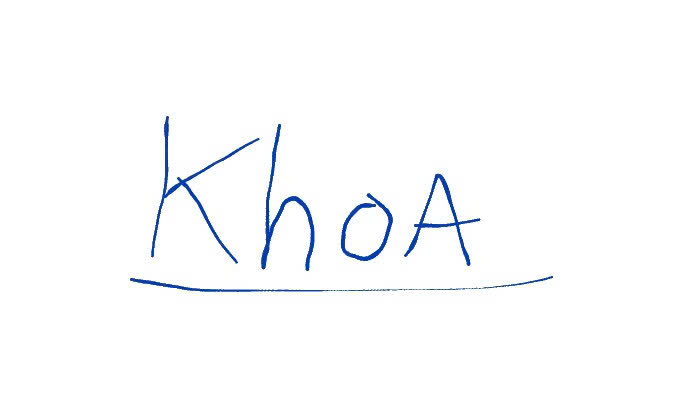
\includegraphics[width=4cm,height=3cm]{Image/signs/khoa.jpg}
\end{tabular}
\end{flushright}

\newpage

\newpage
\section*{Lời cảm ơn}
Lời đầu tiên, chúng em xin trân trọng cảm ơn giảng viên Trần Thị Quế Nguyệt - người đã trực tiếp chỉ bảo, hướng dẫn chúng em trong quá trình hoàn thành đồ án này. Chúng em cũng xin được gửi lời cảm ơn đến quý thầy, cô giáo trường Đại học Bách Khoa – Đại học Quốc gia Thành phố Hồ Chí Minh, đặc biệt là các thầy, cô khoa Khoa học và Kỹ thuật máy tính - những người đã truyền lửa và giảng dạy kiến thức cho chúng em suốt thời gian qua. Trong quá trình thực hiện khó tránh khỏi những thiếu sót, chúng em rất mong nhận được những ý kiến đóng góp quý báu từ quý thầy, cô để đồ án được hoàn thiện hơn. Chúng em xin chân thành cảm ơn!

\newpage
\tableofcontents

% Chuong 1
\newpage
\section{Tổng quan về đề tài}

\subsection{Lý do chọn đề tài}

Trong bối cảnh giáo dục hiện đại, việc rèn luyện tư duy logic và khả năng giải quyết vấn đề cho học sinh tiểu học ngày càng được chú trọng. Toán tư duy không chỉ giúp các em nâng cao năng lực học thuật mà còn là nền tảng quan trọng cho các kỹ năng như phân tích, suy luận và sáng tạo. Tuy nhiên, các hình thức học truyền thống thường khô khan, thiếu tính trực quan và dễ làm giảm hứng thú của học sinh.

Bên cạnh đó, công nghệ giáo dục (EdTech) đang phát triển mạnh mẽ, mở ra cơ hội ứng dụng các phương pháp mới giúp học sinh tiếp cận kiến thức một cách sinh động và hiệu quả hơn. Việc xây dựng một trang web học toán tư duy với giao diện trực quan, hoạt động tương tác và mini-game sinh động sẽ giúp các em vừa học vừa chơi, từ đó tăng khả năng ghi nhớ và phát triển tư duy tự nhiên.

Chính vì vậy, nhóm quyết định lựa chọn đề tài “Website học toán tư duy cho học sinh tiểu học” nhằm tạo ra một công cụ học tập hiện đại, dễ sử dụng, phù hợp với lứa tuổi và có khả năng hỗ trợ việc học tập một cách hiệu quả và thú vị hơn. Đề tài hướng tới việc thu hẹp khoảng cách giữa lý thuyết toán học và ứng dụng thực tiễn thông qua các trải nghiệm số hóa.

\subsection{Thách thức hiện tại}

Việc triển khai các nền tảng giáo dục toán tư duy tại Việt Nam hiện nay vẫn đang đối mặt với nhiều khó khăn, xuất phát từ cả phương pháp tiếp cận lẫn hạ tầng công nghệ. Qua quá trình khảo sát thực trạng học tập của học sinh tiểu học, nhóm đã tổng hợp được các thách thức cốt lõi như sau:

\begin{itemize} \item \textbf{Thiếu môi trường học tập trực quan và tương tác:} Phần lớn tài liệu toán tư duy hiện nay ở dạng sách in hoặc bài tập truyền thống, khiến học sinh khó hình dung, đặc biệt với các bài đòi hỏi suy luận hoặc thao tác trực tiếp. \item \textbf{Khó duy trì hứng thú học tập:} Nội dung học không được game hóa hoặc thiết kế hấp dẫn khiến học sinh dễ chán nản, không duy trì được sự tập trung trong thời gian dài. \item \textbf{Thiếu hệ thống theo dõi tiến trình học tập:} Giáo viên và phụ huynh khó nắm bắt được mức độ hiểu bài của học sinh, tiến trình học hoặc điểm mạnh – điểm yếu để có hướng hỗ trợ kịp thời. \item \textbf{Chưa có công cụ học toán tư duy phù hợp độ tuổi:} Nhiều nền tảng hiện nay thiết kế cho lứa tuổi lớn hơn, sử dụng thuật ngữ phức tạp hoặc giao diện khó sử dụng đối với học sinh tiểu học. \item \textbf{Hạn chế trong việc cá nhân hóa trải nghiệm học:} Mỗi học sinh có khả năng tiếp thu khác nhau, nhưng các tài liệu hiện tại chưa đáp ứng tốt việc tùy chỉnh độ khó hoặc cung cấp gợi ý phù hợp năng lực từng em. \end{itemize}

Những rào cản này không chỉ ảnh hưởng đến hiệu quả tiếp thu của học sinh mà còn tạo ra áp lực cho phụ huynh trong việc kèm cặp. Do đó, việc xác định rõ các thách thức này là cơ sở quan trọng để nhóm đề xuất các tính năng giải quyết triệt để vấn đề trong phần thiết kế hệ thống.

\subsection{Mục tiêu của đề tài}

Mục tiêu tổng quát của đề tài là phát triển một hệ thống học toán tư duy trực tuyến dành riêng cho học sinh tiểu học, giúp các em rèn luyện khả năng suy luận và tư duy logic thông qua các bài học tương tác. Hệ thống được kỳ vọng sẽ tạo ra một môi trường học tập cá nhân hóa, nơi năng lực của từng học sinh được ghi nhận và phát triển theo lộ trình phù hợp. Để đạt được điều đó, đề tài tập trung vào các mục tiêu cụ thể sau:

\begin{itemize} \item Xây dựng các bài học toán tư duy với nội dung trực quan, dễ hiểu, bám sát chương trình giáo dục phổ thông mới của Bộ Giáo dục và Đào tạo Việt Nam. \item Phát triển bộ mini–game tương tác đa dạng trên nền tảng Cocos Creator 3.8, giúp học sinh phát triển tư duy thông qua các thao tác kéo thả, giải đố và tìm quy luật. \item Thiết lập hệ thống Gamification toàn diện bao gồm điểm thưởng, huy hiệu (badges) và bảng xếp hạng để thúc đẩy động lực tự học dựa trên các khung lý thuyết về trò chơi hóa. \item Xây dựng công cụ quản lý dành cho phụ huynh, cho phép theo dõi chi tiết tiến trình học tập, biểu đồ tăng trưởng kỹ năng và thời gian tương tác của con trẻ trên hệ thống. \end{itemize}

Việc hoàn thành các mục tiêu này sẽ mang lại một giải pháp giáo dục toàn diện, không chỉ dừng lại ở việc cung cấp kiến thức mà còn hình thành thói quen tư duy độc lập cho học sinh. Đây là tiền đề để xây dựng một cộng đồng học tập trực tuyến lành mạnh và bền vững.

\subsection{Phạm vi của đề tài}

Để đảm bảo tính khả thi và chất lượng hoàn thiện của hệ thống, đề tài tập trung nghiên cứu và triển khai trong những giới hạn cụ thể. Các nội dung thực hiện được phân định rõ ràng qua bốn khía cạnh chính bao gồm chức năng, kỹ thuật, người dùng và các phần nằm ngoài phạm vi nghiên cứu:

\begin{itemize} \item \textbf{Phạm vi chức năng:} Hệ thống tập trung cung cấp kho bài học tương tác, các mini-game rèn luyện phản xạ toán học và hệ thống báo cáo kết quả tự động. Các tính năng về quản lý tài khoản phụ huynh và cơ chế vinh danh thông qua huy hiệu cũng là trọng tâm của giai đoạn phát triển này.
	
	\item \textbf{Phạm vi kỹ thuật:} Đề tài ứng dụng các công nghệ hiện đại như Next.js cho giao diện người dùng, Node.js và MongoDB cho quản trị dữ liệu backend. Đặc biệt, phần bài tập tương tác được xây dựng chuyên sâu bằng engine Cocos Creator 3.8 để tối ưu hóa trải nghiệm trên trình duyệt.
	
	\item \textbf{Phạm vi người dùng:} Đối tượng phục vụ chính là học sinh tiểu học (từ lớp 1 đến lớp 5) và các phụ huynh tại Việt Nam có nhu cầu sử dụng công cụ học tập bổ trợ bằng tiếng Việt.
	
	\item \textbf{Phạm vi ngoài đề tài:} Trong giai đoạn này, hệ thống sẽ không hỗ trợ tính năng thi đấu trực tuyến thời gian thực (Real-time Battle) giữa nhiều người chơi, không phát triển ứng dụng di động riêng biệt (Native App) và không cung cấp nội dung cho cấp học trung học.
\end{itemize}

% Chuong 2
\newpage
\section{Khảo sát liên quan}
Chương này tập trung phân tích và so sánh ưu, nhược điểm của các giải pháp hiện có trên thị trường. Thông qua đó, những đặc tính ưu việt sẽ được chọn lọc nhằm xác định hướng phát triển tối ưu cho đề tài.

\subsection{So sánh các hệ thống hiện tại trên thị trường}

Để có cơ sở thực tiễn cho việc đề xuất và phát triển giải pháp tại thị trường trong nước, chúng tôi đã tiến hành khảo sát, phân tích và đánh giá một số ứng dụng học toán tư duy đang phổ biến. Kết quả so sánh được tổng hợp trong Bảng \ref{tab:math_learning_apps}, tập trung làm rõ sự tương thích giữa các giải pháp quốc tế với đặc thù giáo dục tại Việt Nam.

\begin{table}[h!]
	\centering
	\small
	\renewcommand{\arraystretch}{1.2}
	\resizebox{\textwidth}{!}{%
		\begin{tabular}{|l|p{3.5cm}|p{2.5cm}|p{2cm}|p{2cm}|p{3cm}|p{3.5cm}|}
			\hline
			\textbf{Tên Ứng dụng} & \textbf{Tính năng nổi bật} & \textbf{Đối tượng phù hợp} & \textbf{Ngôn ngữ} & \textbf{Mức phí} & \textbf{Nội dung toán tư duy} & \textbf{Hạn chế tại VN} \\
			\hline
			
			\textbf{Khan Academy Kids} & 
			Video giảng giải chi tiết. \newline 
			Hoạt hình sinh động. & 
			Học sinh có khả năng ngoại ngữ tốt. & 
			Tiếng Anh. & 
			\textbf{Miễn phí}. & 
			Phong phú, chuẩn quốc tế. & 
			Rào cản ngôn ngữ rất lớn; nội dung chưa đúng với khung chương trình Bộ GD\&ĐT Việt Nam. \\
			\hline
			
			\textbf{Duolingo Math} & 
			Game hóa (streak, bảng xếp hạng). & 
			Học sinh muốn học toán kết hợp tiếng Anh. & 
			Tiếng Anh. & 
			Miễn phí cơ bản. & 
			Cơ bản, thiên về luyện tập nhanh. & 
			Chưa hỗ trợ tiếng Việt; thiếu các dạng toán đố, toán tư duy đặc thù của Việt Nam. \\
			\hline
			
			\textbf{Kurio} & 
			Học đa lĩnh vực (Toán, Khoa học). & 
			Học sinh Việt Nam cần kiến thức tổng hợp. & 
			Tiếng Việt. & 
			Có phí. & 
			Nhiều chủ đề nhưng chưa sâu. & 
			Nội dung toán tư duy chưa được chuyên sâu hóa; mức độ tương tác game còn thấp. \\
			\hline
			
			\textbf{VioEdu} & 
			Bám sát SGK Việt Nam. \newline Đấu trường toán học. & 
			Học sinh cần luyện thi và học trên lớp. & 
			Tiếng Việt. & 
			Có phí. & 
			Chủ yếu theo sát chương trình học chính khóa. & 
			Thiên về điểm số và luyện bài tập; thiếu hụt các chuyên đề tư duy logic mở rộng. \\
			\hline
			
			\textbf{Matific} & 
			Học qua mini-game tương tác cao. & 
			Học sinh thích trải nghiệm quốc tế. & 
			Đa ngôn ngữ (hạn chế tiếng Việt). & 
			Phí cao. & 
			Rất sâu sắc về bản chất toán học. & 
			Chi phí đăng ký cao so với thu nhập bình quân tại VN; rào cản về thanh toán quốc tế. \\
			\hline
		\end{tabular}%
	}
	\caption{Bảng so sánh các ứng dụng học toán tư duy cho học sinh tiểu học trong bối cảnh Việt Nam}
	\label{tab:math_learning_apps}
\end{table}

\subsection{Điểm mạnh và điểm yếu của các giải pháp hiện có tại Việt Nam}

Kết quả khảo sát cho thấy bức tranh chung về thị trường ứng dụng giáo dục toán học tại Việt Nam như sau:

\textbf{Điểm mạnh:}
\begin{itemize}
	\item Các ứng dụng nội địa (VioEdu) có ưu thế tuyệt đối về việc bám sát nội dung kiểm tra, đánh giá theo chương trình giáo dục phổ thông của Việt Nam.
	\item Các ứng dụng quốc tế mang lại trải nghiệm người dùng xuất sắc, giúp học sinh tiếp cận toán học dưới góc nhìn trực quan và hiện đại.
\end{itemize}

\textbf{Điểm yếu và hạn chế đặc thù tại Việt Nam:}
\begin{itemize}
	\item \textbf{Sự tách rời giữa "Toán tư duy" và "Toán SGK":} Hiện nay học sinh Việt Nam thường phải chọn một trong hai: hoặc học bám sát chương trình trên lớp nhưng khô khan, hoặc học toán tư duy quốc tế nhưng lại không hỗ trợ được cho các kỳ thi tại trường.
	\item \textbf{Rào cản ngôn ngữ và địa lý:} Các ứng dụng chất lượng hàng đầu thế giới hầu như chưa được Việt hóa hoàn toàn, gây khó khăn cho học sinh ở các vùng tỉnh lẻ hoặc những gia đình chưa chú trọng tiếng Anh sớm.
	\item \textbf{Chi phí tiếp cận:} Các nền tảng học tập chất lượng cao thường có mức giá chưa phù hợp với điều kiện kinh tế của đại đa số gia đình Việt Nam, đặc biệt là ở phân khúc phổ thông.
\end{itemize}

\subsection{Giải pháp đề xuất}

Để giải quyết các bài toán trên, hệ thống học toán tư duy tập trung vào việc \textbf{bản địa hóa trải nghiệm quốc tế} và \textbf{nâng tầm chương trình nội địa}:

\begin{itemize}
	\item \textbf{Nội dung được thiết kế cho học sinh Việt:} Xây dựng hệ thống bài học vừa đảm bảo bám sát chương trình của Bộ Giáo dục và Đào tạo, vừa tích hợp các chuyên đề tư duy logic (Math Logic) theo tiêu chuẩn quốc tế nhưng hoàn toàn bằng tiếng Việt.
	\item \textbf{Game hóa thuần Việt:} Thiết kế giao diện và các thử thách học tập gần gũi với văn hóa, tâm lý của trẻ em Việt Nam, giúp tạo động lực tự học mà không cần sự ép buộc từ phụ huynh.
	\item \textbf{Cá nhân hóa theo năng lực thực tế:} Hệ thống chẩn đoán trình độ dựa trên mặt bằng kiến thức chung của học sinh trong nước, từ đó đưa ra lộ trình bù đắp lỗ hổng kiến thức kịp thời.
	\item \textbf{Hỗ trợ phụ huynh tối đa:} Cung cấp kênh báo cáo tự động qua các nền tảng phổ biến tại Việt Nam, giúp phụ huynh nắm bắt điểm mạnh/yếu của con mình một cách khoa học mà không cần giỏi chuyên môn toán.
	\item \textbf{Khả năng phổ cập:} Hướng tới mục tiêu giúp mọi trẻ em Việt Nam, dù ở thành thị hay nông thôn, đều có cơ hội tiếp cận phương pháp học toán tư duy hiện đại với mức chi phí tối thiểu hoặc miễn phí.
\end{itemize}

% Chuong 3
\newpage
\section{Phân tích yêu cầu}
\subsection{Yêu cầu chức năng}
\begin{itemize}
    \item \textbf{Yêu cầu chung cho người dùng}
    \begin{itemize}
        \item Người dùng có thể đăng nhập và đăng ký tài khoản.
        \item Người dùng có thể xem và chỉnh sửa hồ sơ cá nhân.
        \item Người dùng có thể thay đổi mật khẩu và khôi phục lại mật khẩu khi quên.
    \end{itemize}
    
    \item \textbf{Đối với học sinh}
    \begin{itemize}
        \item Học sinh có thể học toán thông qua các bài tập dạng tương tác (kéo thả, nối, trắc nghiệm, điền khuyết, tô màu, đúng/sai,...)
        \item Học sinh có thể tham gia làm bài thi Đấu trường hằng tuần và tích lũy điểm để nâng cấp bậc xếp hạng.
        \item Học sinh có thể chơi các trò chơi toán học tư duy (chơi đơn hoặc tương tác cùng phụ huynh).
        \item Học sinh có thể theo dõi tiến độ học tập và lịch sử làm bài.
        \item Học sinh có thể thực hiện các nhiệm vụ hằng ngày và nhận thưởng.
        \item Học sinh có thể theo dõi bảng xếp hạng học tập và bảng xếp hạng đấu trường.
        \item Học sinh có thể làm bài kiểm tra đầu vào để đánh giá năng lực hiện tại.
        \item Học sinh có thể liên kết tài khoản với phụ huynh (Nhập mã mời hoặc gửi yêu cầu).
    \end{itemize}
    
    \item \textbf{Đối với phụ huynh}
    \begin{itemize}
        \item Phụ huynh có thể theo dõi tiến độ và kết quả học tập của con.
        \item Phụ huynh có thể liên kết tài khoản với học sinh (Gửi yêu cầu liên kết).
        \item Phụ huynh có thể nâng cấp tài khoản cho bản thân và cho các tài khoản học sinh được liên kết.
    \end{itemize}
  \item \textbf{Đối với quản trị viên (Admin)}
  \begin{itemize}
  	\item Quản trị viên có thể quản lý tài khoản người dùng (xem danh sách, khoá/mở tài khoản).
  	\item Quản trị viên có thể quản lý chương trình học (tạo, chỉnh sửa, xoá nội dung học, tổ chức theo chủ đề/bài học).
  	\item Quản trị viên có thể quản lý nhiệm vụ (tạo nhiệm vụ hằng ngày, thiết lập điều kiện hoàn thành và phần thưởng).
  	\item Quản trị viên có thể quản lý minigames (tạo, chỉnh sửa nội dung game)
  	\item Quản trị viên có thể quản lý tài chính
  	\begin{itemize}
  		\item Xem doanh thu của hệ thống.
  		\item Theo dõi và quản lý các giao dịch thanh toán.
  	\end{itemize}
  \end{itemize}
\end{itemize}


\subsection{Yêu cầu phi chức năng}

\subsubsection{Hiệu năng}
\begin{itemize}[leftmargin=2.0cm]2
	\item Thời gian tải trang chính $\leq 3$ giây với kết nối Internet ổn định.
	\item Hệ thống phản hồi các thao tác người dùng trong thời gian $\leq 1$ giây.
	\item Kết quả bài tập và biểu đồ tiến độ được cập nhật gần thời gian thực.
\end{itemize}

\subsubsection{Bảo mật}
\begin{itemize}[leftmargin=2.0cm]
	\item Người dùng chỉ được truy cập và thao tác trên dữ liệu cá nhân của mình.
	\item Hệ thống áp dụng cơ chế xác thực và phân quyền người dùng.
	\item Dữ liệu truyền tải giữa trình duyệt và máy chủ được mã hóa bằng HTTPS.
\end{itemize}

\subsubsection{Tính khả dụng và Độ tin cậy}
\begin{itemize}[leftmargin=2.0cm]
	\item Hệ thống đảm bảo thời gian hoạt động (uptime) tối thiểu 99\%.
	\item Dữ liệu được sao lưu tự động định kỳ mỗi 24 giờ.
	\item Có cơ chế khôi phục hệ thống trong vòng 30 phút sau sự cố.
\end{itemize}

\subsubsection{Khả năng mở rộng}
\begin{itemize}[leftmargin=2.0cm]
	\item Hệ thống có khả năng phục vụ đồng thời tối thiểu 500 người dùng.
	\item Kiến trúc cho phép mở rộng theo chiều ngang khi số lượng người dùng tăng.
	\item Dễ dàng tích hợp hoặc bổ sung các tính năng và nội dung mới.
\end{itemize}

\subsubsection{Tính dễ sử dụng}
\begin{itemize}[leftmargin=2.0cm]
	\item Giao diện trực quan, thân thiện, phù hợp với học sinh.
	\item Người dùng mới có thể hoàn thành bài tập đầu tiên trong thời gian $\leq 2$ phút.
	\item Hệ thống hỗ trợ hướng dẫn sử dụng và phản hồi trực quan.
\end{itemize}

\subsubsection{Tương thích}
\begin{itemize}[leftmargin=2.0cm]
	\item Ứng dụng tương thích với các trình duyệt phổ biến như Chrome, Firefox, Edge và Safari.
	\item Giao diện hỗ trợ hiển thị tốt trên máy tính, máy tính bảng và thiết bị di động (responsive).
\end{itemize}

\subsubsection{Khả năng bảo trì}
\begin{itemize}[leftmargin=2.0cm]
	\item Mã nguồn được tổ chức rõ ràng, dễ bảo trì và mở rộng.
	\item Các bản cập nhật được triển khai thông qua quy trình CI/CD.
	\item Lỗi nghiêm trọng được phát hiện và khắc phục trong vòng 24 giờ.
\end{itemize}

\subsubsection{Khả năng triển khai linh hoạt}
\begin{itemize}[leftmargin=2.0cm]
	\item Backend có thể triển khai trên nhiều nền tảng hạ tầng đám mây khác nhau.
	\item Hệ thống hỗ trợ triển khai độc lập giữa frontend và backend.
\end{itemize}

\subsubsection{Quyền riêng tư và Tuân thủ}
\begin{itemize}[leftmargin=2.0cm]
	\item Không chia sẻ dữ liệu người dùng cho bên thứ ba khi chưa có sự đồng ý.
	\item Cung cấp chức năng xóa tài khoản và toàn bộ dữ liệu theo yêu cầu của người dùng.
	\item Tuân thủ các quy định về bảo vệ dữ liệu cá nhân.
\end{itemize}


\subsection{Các tác nhân hệ thống}

Quá trình phát triển website \textbf{Dino} bao gồm các bên liên quan chính như sau:

\subsubsection{Người dùng cuối (End-users)}
\begin{itemize}
\item Học sinh tiểu học tham gia các trò chơi và bài tập toán tư duy.
\item Phụ huynh quan tâm đến việc cải thiện khả năng tư duy và kỹ năng toán học của con.
\item Phụ huynh muốn theo dõi tiến độ học tập và đánh giá kỹ năng của học sinh.
\end{itemize}

\subsubsection{Nhà phát triển và đội ngũ kỹ thuật (Development \& Technical Team)}
\begin{itemize}
\item \textbf{Product Owner / Product Manager}: xác định yêu cầu, định hướng phát triển nội dung giáo dục và trải nghiệm người dùng.
\item \textbf{Developers (Frontend, Backend)}: xây dựng và phát triển website, các trò chơi và bài tập tương tác.
\item \textbf{UI/UX Designers}: thiết kế giao diện trực quan, phù hợp với trẻ em, dễ sử dụng.
\item \textbf{QA / Testers}: kiểm thử tính năng, đảm bảo các bài tập và trò chơi hoạt động ổn định.
\end{itemize}

\subsubsection{Đối tác công nghệ (Technology Partners)}
\begin{itemize}
\item \textbf{Dịch vụ thanh toán}: hỗ trợ các giao dịch mua nội dung, gói học tập hoặc nâng cấp tài khoản.
\item \textbf{Dịch vụ bảo mật / xác thực}: đảm bảo an toàn dữ liệu học sinh, phụ huynh
\end{itemize}

% Chuong 4
\newpage
\section{Phân tích và thiết kế hệ thống}
Chương này tập trung trình bày về các use-case, quy trình nghiệp vụ của những chức năng cơ bản và thiết kế tổng quan cho kiến trúc hệ thống. Đây là cơ sở quan trọng giúp định hình trực tiếp quá trình xây dựng và phát triển hệ thống cả về mặt kĩ thuật lẫn nghiệp vụ.

\subsection{Sơ đồ usecase}
\begin{figure}[H]
	\centering
	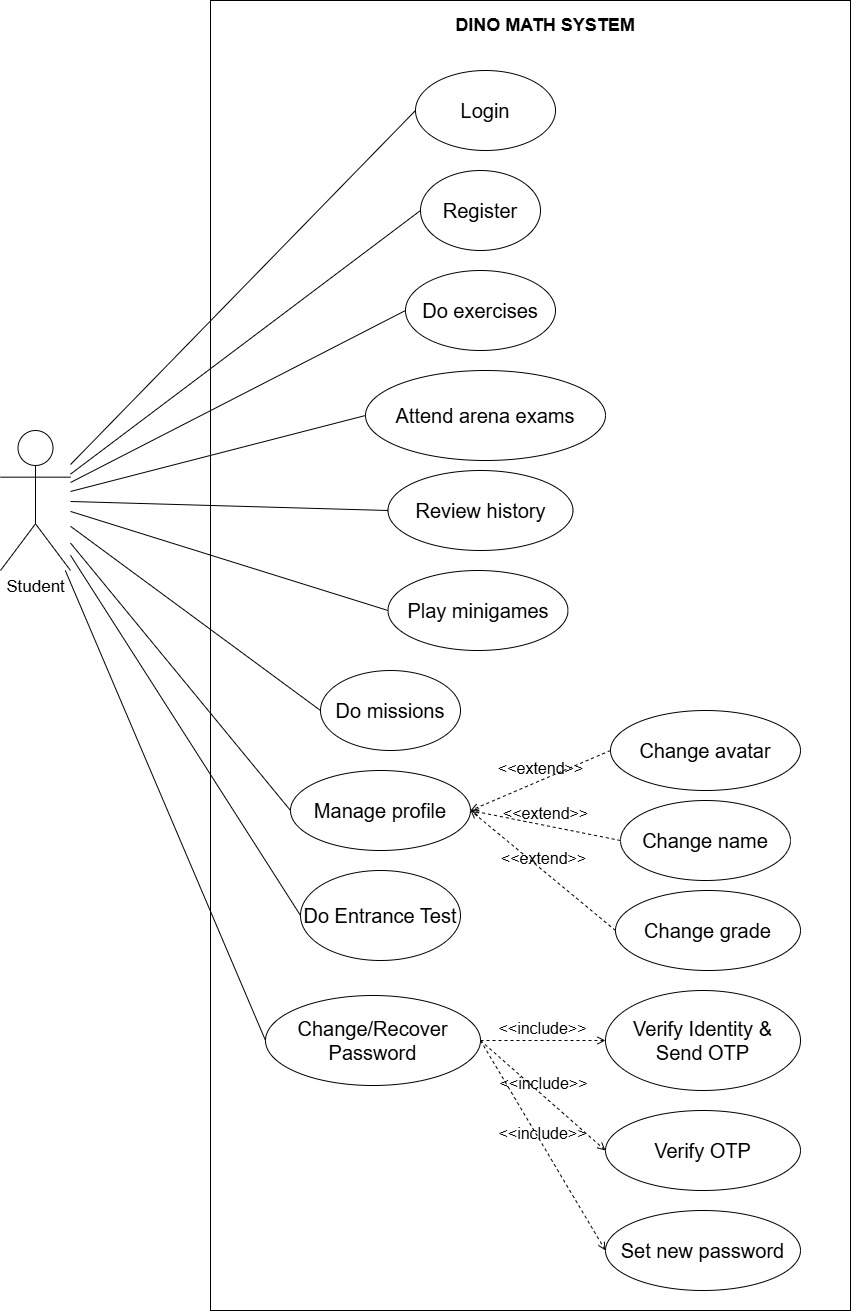
\includegraphics[width=0.8\textwidth]{Image/Diagrams/Usecase/StudentUseCase.jpg}
	\vspace{0.6cm}
	\caption{Usecase Diagram - Học sinh}
	\label{fig:studentuc}
\end{figure}
\begin{figure}[H]
	\centering
	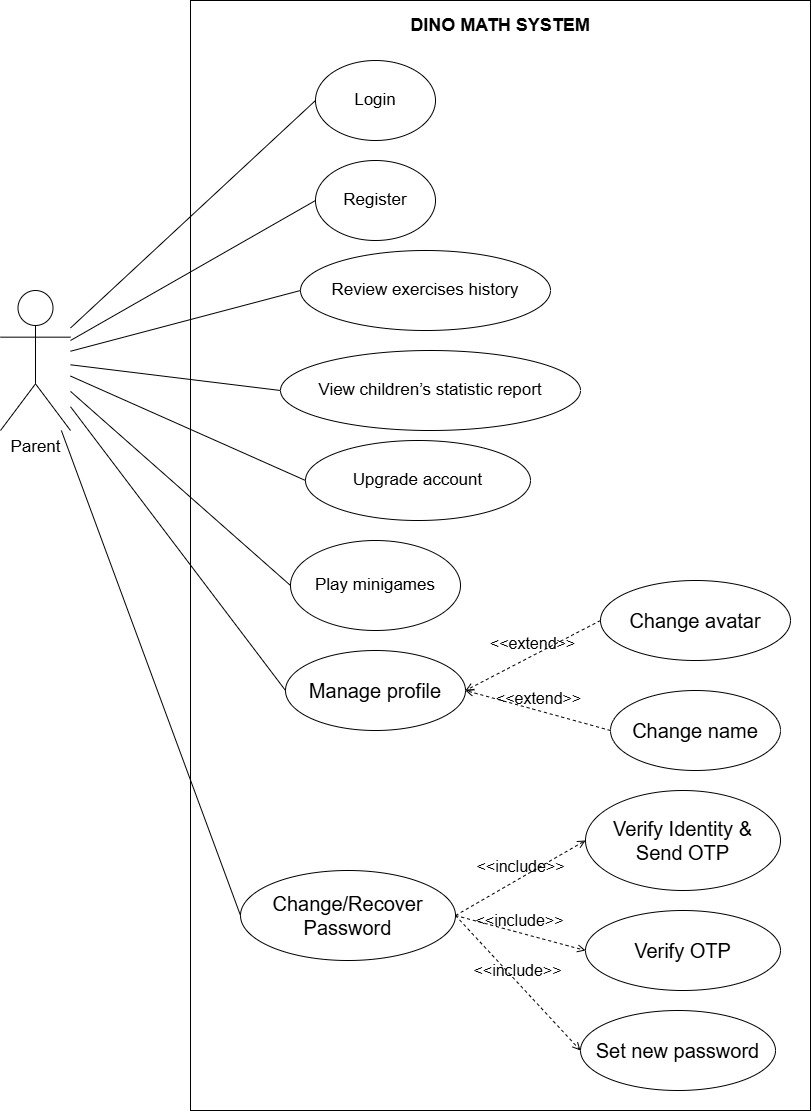
\includegraphics[width=0.8\textwidth]{Image/Diagrams/Usecase/ParentUseCase.jpg}
	\vspace{0.6cm}
	\caption{Usecase Diagram -  Phụ huynh}
	\label{fig:parentuc}
\end{figure}
\begin{figure}[H]
	\centering
	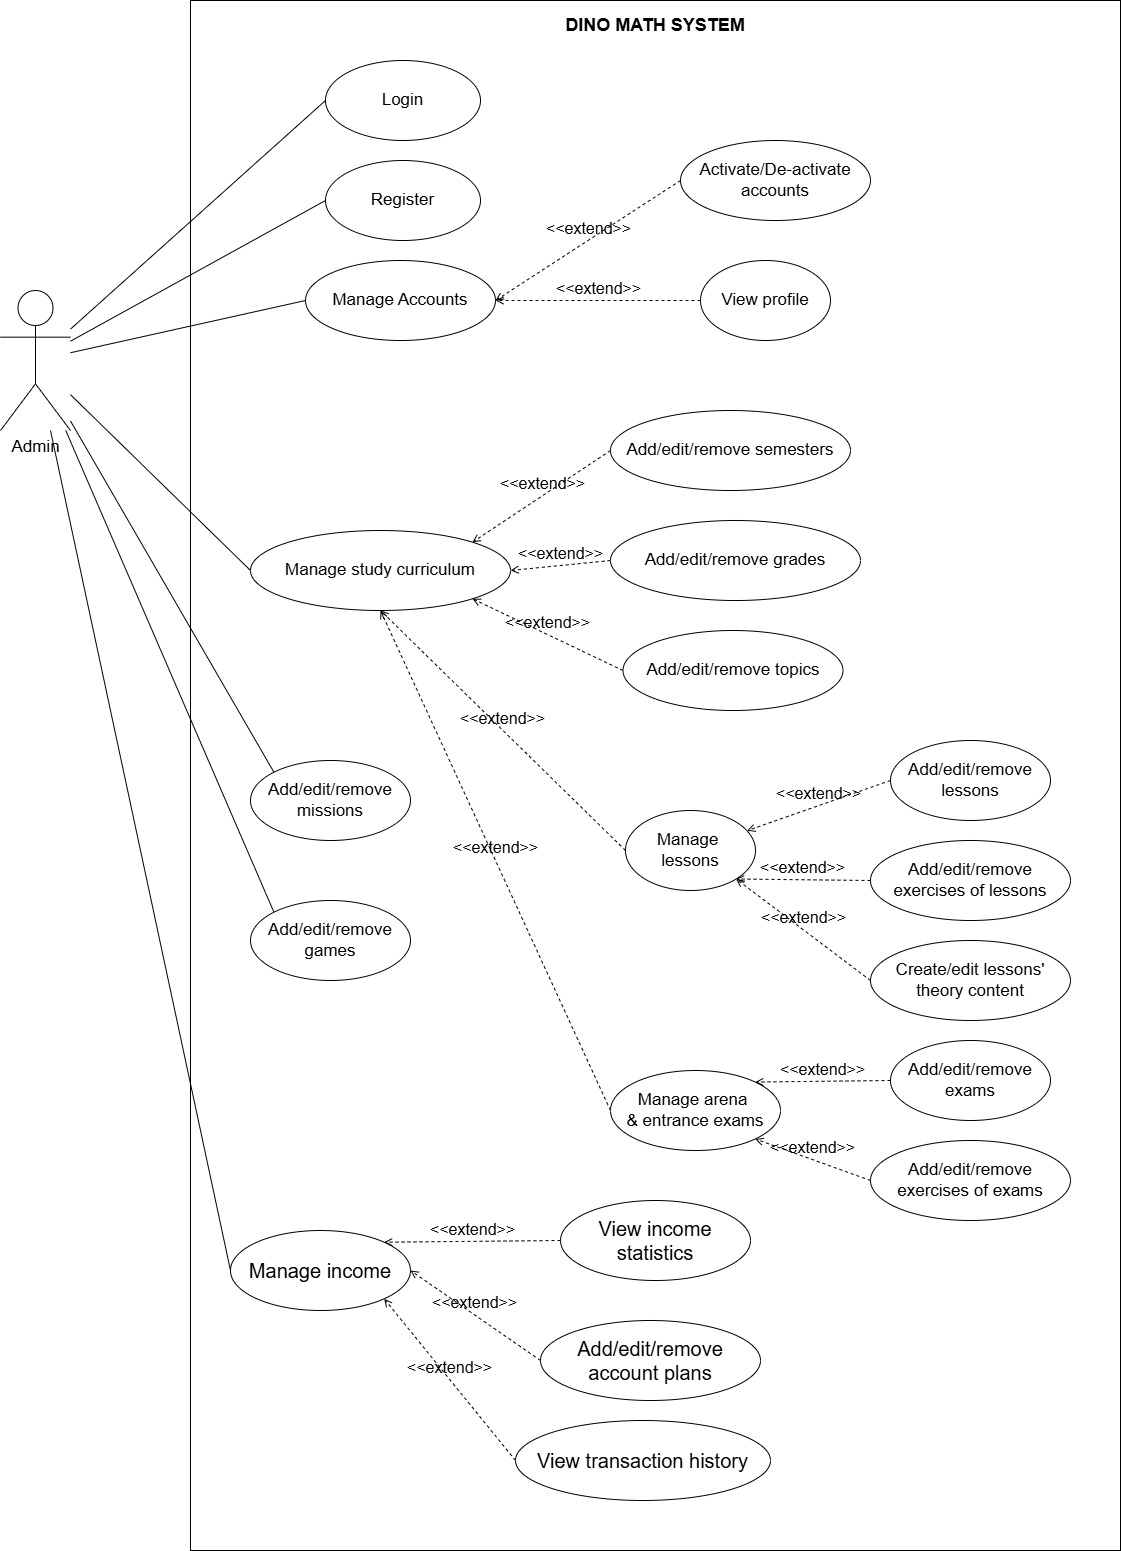
\includegraphics[width=0.9\textwidth]{Image/Diagrams/Usecase/AdminUsecase.jpg}
	\vspace{0.6cm}
	\caption{Usecase Diagram - Admin}
	\label{fig:adminuc}
\end{figure}

\subsection{Mô tả chi tiết}
\subsubsection{Đăng nhập (Login)}
\begin{table}[H]
  \centering
  \renewcommand{\arraystretch}{1.3}
  \begin{tabular}{|l|p{0.75\textwidth}|}
    \hline
    \textbf{Usecase name} & Login \\ \hline
    \textbf{Actor} & End-user \\ \hline
    \textbf{Description} & Cho phép end-user truy cập vào hệ thống bằng cách xác thực danh tính của họ. \\ \hline
    \textbf{Precondition} & End-user đã có tài khoản hợp lệ trên hệ thống. \\ \hline
    \textbf{Postcondition} & End-user được xác thực thành công và được chuyển đến màn hình chính của hệ thống. \\ \hline
    \textbf{Main flow} &
    1. End-user truy cập vào màn hình đăng nhập. \newline
    2. Hệ thống hiển thị giao diện đăng nhập. \newline
    3. End-user nhập username và password. \newline
    4. End-user nhấn nút Login. \newline
    5. Hệ thống xác thực thông tin đăng nhập. \newline
    6. Hệ thống chuyển end-user đến màn hình chính. \\ \hline
    \textbf{Alternative flow} &
    \textit{Alternative flow 1: Quên mật khẩu} \newline
    Bước 3: End-user nhấn vào "Forgot password?". \newline
    Hệ thống chuyển hướng đến màn hình Quên mật khẩu. \\ \hline
    \textbf{Exception} &
    \textit{Exception 1: Dữ liệu không hợp lệ} \newline
    Tại bước 5: Hệ thống hiển thị thông báo lỗi và yêu cầu end-user nhập lại. \newline\newline
    \textit{Exception 2: Thông tin đăng nhập không đúng} \newline
    Tại bước 5: Hệ thống hiển thị thông báo lỗi và yêu cầu end-user nhập lại. \\ \hline
  \end{tabular}
  \caption{Usecase - Login}
  \label{table:uc_acc01}
\end{table}
\newpage
\begin{figure}[H]
  \centering
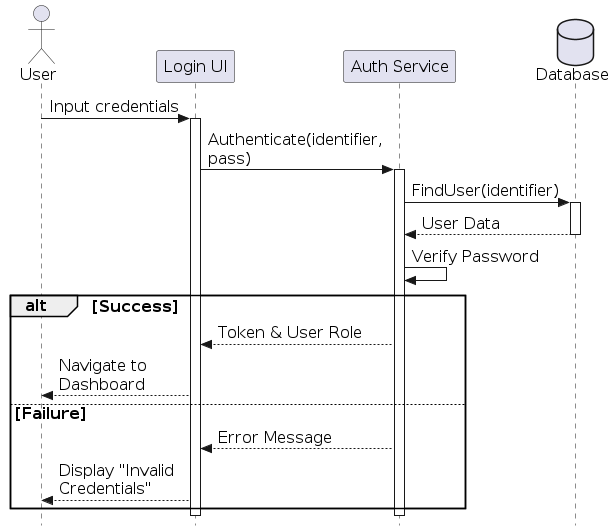
\includegraphics[width=0.8\textwidth]{Image/Diagrams/Sequence/LoginSequence.png}
  \vspace{1.0cm}
  \caption{Sequence diagram - Login}
\end{figure}
\newpage
\begin{figure}[H]
  \centering
   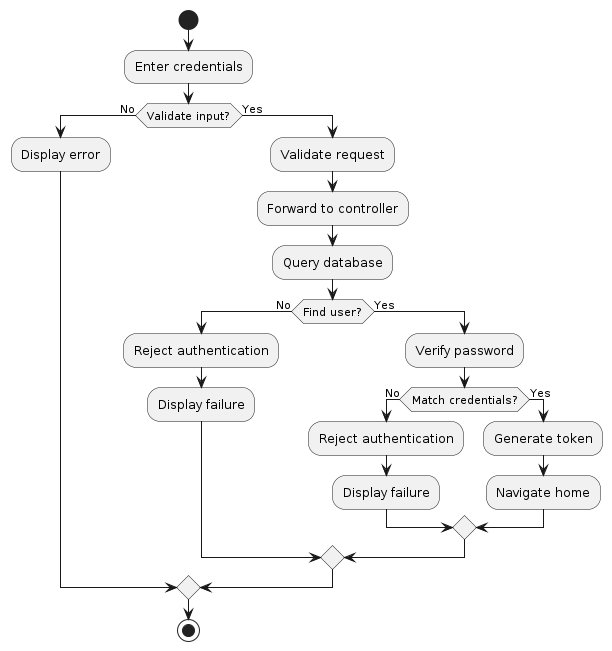
\includegraphics[width=0.9\textwidth]{Image/Diagrams/Activity/LoginActivity.png}
   \vspace{0.6cm}
  \caption{Activity diagram - Login}
\end{figure}

\newpage
\subsubsection{Đăng ký (Register)}
\begin{table}[H]
  \centering
  \renewcommand{\arraystretch}{1.3}
  \begin{tabular}{|l|p{0.75\textwidth}|}
    \hline
    \textbf{Usecase name} & Register \\ \hline
    \textbf{Actor} & End-user \\ \hline
    \textbf{Description} & Cho phép end-user tạo tài khoản mới để truy cập vào hệ thống. \\ \hline
    \textbf{Precondition} & End-user chưa có tài khoản trên hệ thống. \\ \hline
    \textbf{Postcondition} & Tài khoản mới được tạo thành công với vai trò được chọn và end-user có thể đăng nhập vào hệ thống. \\ \hline
    \textbf{Main flow} &
    1. End-user truy cập vào màn hình đăng ký. \newline
    2. Hệ thống hiển thị giao diện đăng ký. \newline
    3. Chọn vai trò (role): học sinh hoặc phụ huynh \newline
    4. End-user nhập username (đối với học sinh) hoặc email và họ tên (đối với phụ huynh), mật khẩu, xác nhận mật khẩu. \newline
    5. End-user nhấn nút Register. \newline
    7. Hệ thống xác thực dữ liệu đầu vào. \newline
    8. Hệ thống tạo tài khoản mới với vai trò đã chọn. \newline
    9. Hệ thống hiển thị thông báo đăng ký thành công. \\ \hline
    \textbf{Alternative flow} &
    \textit{Alternative flow 1: Quay về Landing Page} \newline
Bước 3: End-user nhấn vào "Quay lại". \newline
    Hệ thống chuyển hướng đến màn hình Landing Page. \\ \hline
    \textbf{Exception} &
    \textit{Exception 1: Dữ liệu không hợp lệ} \newline
    Tại bước 5: Hệ thống hiển thị thông báo lỗi validation và yêu cầu end-user nhập lại. \newline\newline
    \textit{Exception 2: User đã tồn tại} \newline
    Tại bước 6: Hệ thống kiểm tra và phát hiện username hoặc email đã được sử dụng, hiển thị thông báo lỗi và yêu cầu end-user nhập thông tin khác. \\ \hline
  \end{tabular}
  \caption{Usecase - Register}
  \label{table:uc_signup}
\end{table}
\newpage
\begin{figure}[H]
  \centering
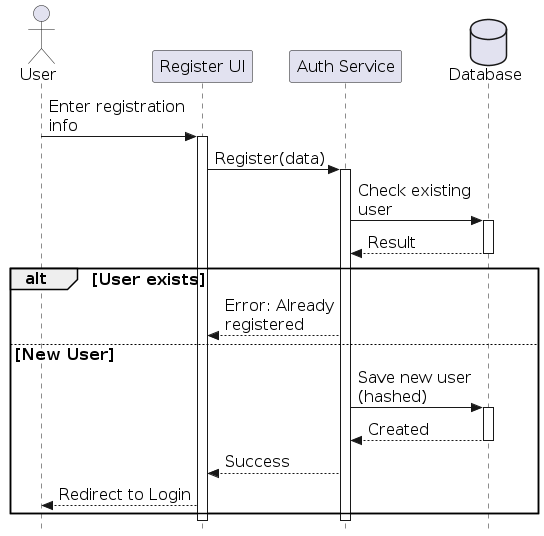
\includegraphics[width=0.8\textwidth]{Image/Diagrams/Sequence/RegisterSequence.png}
  \vspace{1.0cm}
  \caption{Sequence diagram - Register}
\end{figure}
\newpage
\begin{figure}[H]
  \centering
  \begin{adjustbox}{max height=0.9\textheight}
    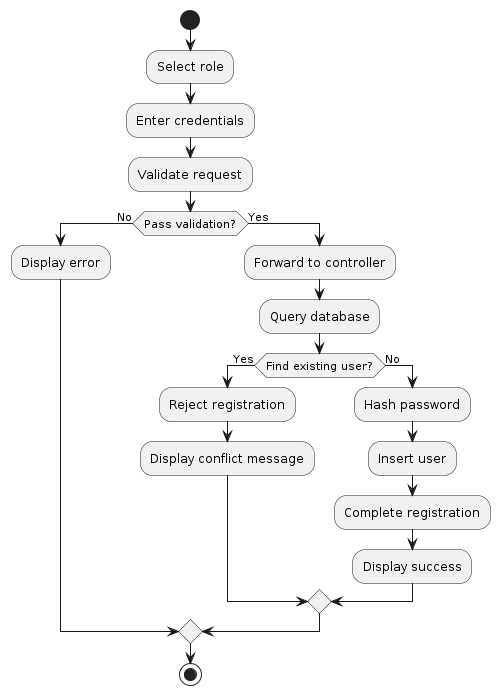
\includegraphics{Image/Diagrams/Activity/RegisterActivity.png}
  \end{adjustbox}
   \vspace{0.6cm}
  \caption{Activity diagram - Register}
\end{figure}
\newpage

\subsubsection{Làm bài tập (Do exercises)}
\begin{table}[H]
  \centering
  \renewcommand{\arraystretch}{1.3}
  \begin{tabular}{|l|p{0.75\textwidth}|}
    \hline
    \textbf{Usecase name} & Do Exercise \\ \hline

    \textbf{Actor} & Student \\ \hline

    \textbf{Description} & 
    Cho phép Student trả lời câu hỏi của bài tập, nhận kết quả đúng/sai, xem đáp án đúng và được hệ thống lưu lại lịch sử làm bài. \\ \hline

    \textbf{Precondition} & 
    Student đã đăng nhập và truy cập vào một bài tập hợp lệ. \\ \hline

    \textbf{Postcondition} & 
    Hệ thống ghi nhận kết quả làm bài, cập nhật điểm (nếu đúng), lưu lịch sử và hiển thị thông báo kết quả cho end-user. \\ \hline

    \textbf{Main flow} &
    1. Student mở bài tập trên màn hình làm bài. \newline
    2. Hệ thống hiển thị danh sách câu hỏi và giao diện trả lời. \newline
    3. Student chọn hoặc nhập câu trả lời cho một câu hỏi. \newline
    4. Student nhấn nút Submit. \newline
    5. Hệ thống kiểm tra tính hợp lệ của dữ liệu gửi lên. \newline
    6. Hệ thống so sánh câu trả lời của Student với đáp án đúng. \newline
    7. Hệ thống lưu kết quả vào lịch sử làm bài. \newline
    8. Nếu câu trả lời đúng, hệ thống cập nhật điểm thưởng. \newline
    9. Hệ thống trả về kết quả đúng/sai cho Student. \newline
    10. Student xem kết quả hiển thị trên màn hình. \\ \hline

    \textbf{Alternative flow} &
    \textit{Alternative flow 1: Xem đáp án đúng} \newline
    Sau bước 9: Student nhấn "View correct answer". \newline
    Hệ thống hiển thị đáp án đúng cho câu hỏi. \\ \hline

    \textbf{Exception} &
    \textit{Exception 1: Dữ liệu không hợp lệ} \newline
    Tại bước 5: Hệ thống trả về thông báo lỗi và yêu cầu Student kiểm tra lại dữ liệu. \newline\newline

    \textit{Exception 2: Câu trả lời sai} \newline
    Tại bước 6: Hệ thống trả về thông báo “Sai”, cho phép Student xem đáp án đúng. \\ \hline
  \end{tabular}
  \caption{Usecase - Do Exercise}
  \label{table:uc_acc02}
\end{table}
\newpage
\begin{figure}[H]
  \centering
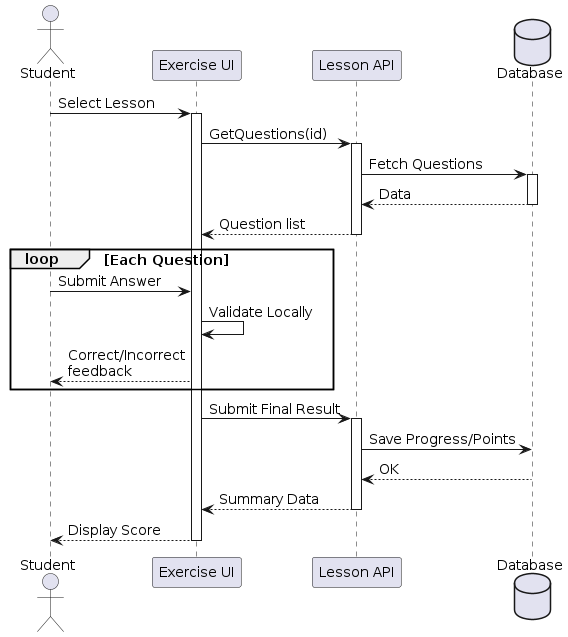
\includegraphics[width=0.8\textwidth]{Image/Diagrams/Sequence/DoExerciseSequence.png}
  \vspace{1.0cm}
  \caption{Sequence diagram - Do exercise}
\end{figure}
\newpage
\begin{figure}[H]
  \centering
  \begin{adjustbox}{max height=0.9\textheight}
    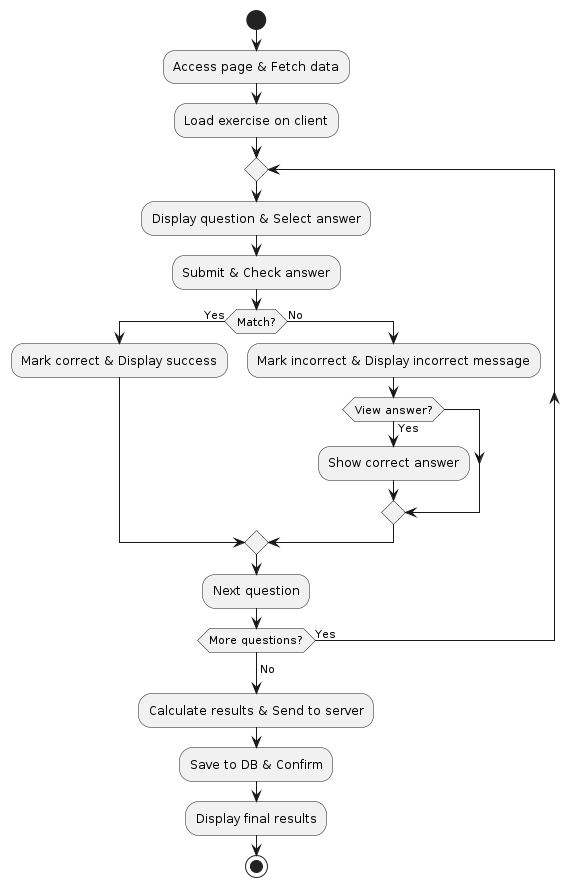
\includegraphics{Image/Diagrams/Activity/ExerciseActivity.png}
  \end{adjustbox}
   \vspace{0.6cm}
  \caption{Activity diagram - Do exercise}
\end{figure}

\subsubsection{Tham gia đấu trường (Join arena)}
\begin{table}[H]
\centering
\renewcommand{\arraystretch}{1.3}
\begin{tabular}{|l|p{0.75\textwidth}|}
\hline
\textbf{Usecase name} & Join Arena \\
\hline
\textbf{Actor} & Student \\
\hline
\textbf{Description} & Cho phép Student tham gia vào một arena để làm bài thi. \\
\hline
\textbf{Precondition} & Student đã đăng nhập vào hệ thống và có arena khả dụng. \\
\hline
\textbf{Postcondition} & Student hoàn thành bài thi arena và kết quả được lưu vào hệ thống. \\
\hline
\textbf{Main flow} & 
1. Student truy cập vào màn hình arena. \newline
2. Hệ thống lấy thông tin arena đang hoạt động (tuần hiện tại). \newline
3. Hệ thống kiểm tra trạng thái arena và trạng thái nộp bài của Student. \newline
4. Hệ thống hiển thị thông tin arena và thời gian còn lại. \newline
5. Student nhấn nút bắt đầu làm bài thi. \newline
6. Hệ thống tải câu hỏi (từ dễ đến khó). \newline
7. Hệ thống hiển thị các câu hỏi. \newline
8. Student trả lời các câu hỏi và nộp bài. \newline
9. Hệ thống validate yêu cầu nộp bài. \newline
10. Hệ thống kiểm tra trạng thái nộp bài. \newline
11. Hệ thống chấm điểm câu trả lời. \newline
12. Hệ thống tính điểm số và thời gian hoàn thành. \newline
13. Hệ thống lưu kết quả nộp bài (điểm, thời gian). \newline
14. Hệ thống cập nhật bảng xếp hạng. \newline
15. Hệ thống hiển thị điểm số và xếp hạng cho Student. \\
\hline
\textbf{Alternative flow} & 
\textit{Alternative flow 1: Arena đã hết hạn hoặc Student đã nộp bài} \newline
Tại bước 3: Hệ thống phát hiện arena đã hết hạn hoặc Student đã nộp bài trước đó. \newline
Hệ thống hiển thị thông báo "Arena đã đóng" hoặc "Đã nộp bài". \newline
Usecase kết thúc. \\
\hline
\textbf{Exception} & 
\textit{Exception 1: Dữ liệu nộp bài không hợp lệ} \newline
Tại bước 9: Hệ thống phát hiện dữ liệu yêu cầu không hợp lệ. \newline
Hệ thống hiển thị thông báo lỗi validation. \newline
Usecase kết thúc. \newline\newline
\textit{Exception 2: Student đã nộp bài trước đó} \newline
Tại bước 10: Hệ thống phát hiện Student đã nộp bài arena này trước đó. \newline
Hệ thống hiển thị thông báo "Đã nộp bài". \newline
Usecase kết thúc. \\
\hline
\end{tabular}
\caption{Usecase - Join Arena}
\label{table:uc_joinarena}
\end{table}

\newpage
\begin{figure}[H]
\centering
\begin{adjustbox}{max height=0.9\textheight}
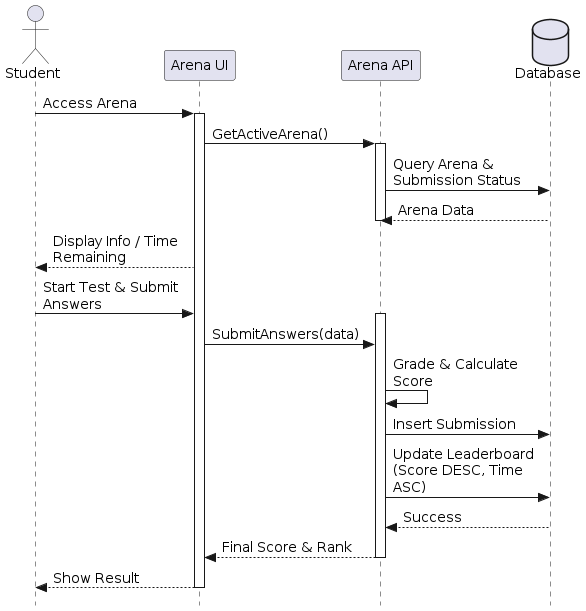
\includegraphics[width=0.8\textwidth]{Image/Diagrams/Sequence/ArenaSequence.png}
\end{adjustbox}
\vspace{1.0cm}
\caption{Sequence diagram - Join Arena}
\end{figure}

\newpage
\begin{figure}[H]
\centering
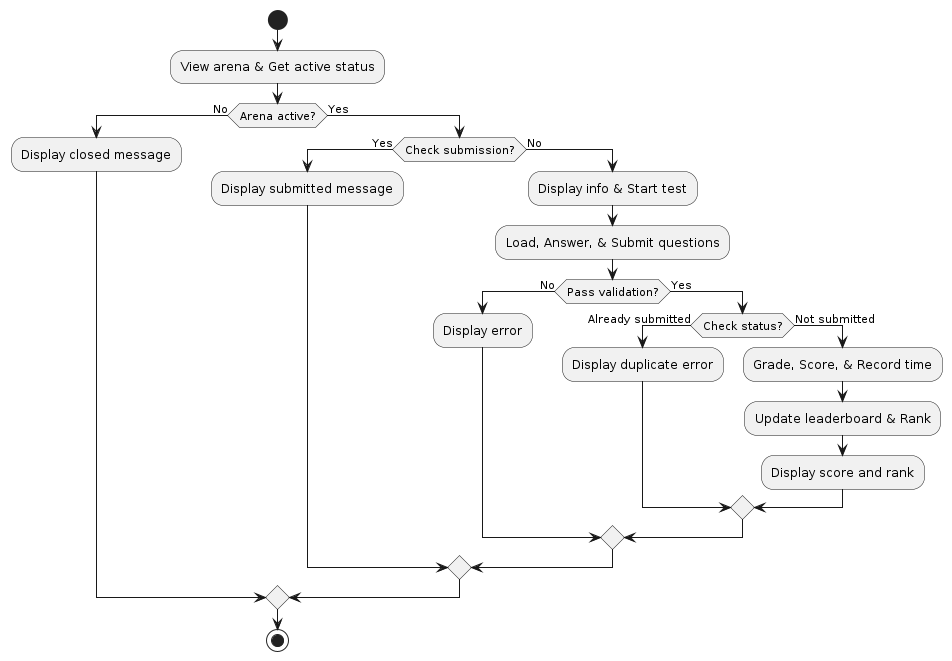
\includegraphics[width=0.9\textwidth]{Image/Diagrams/Activity/ArenaActivity.png}
\vspace{0.6cm}
\caption{Activity diagram - Join Arena}
\end{figure}

\subsubsection{Xem lịch sử làm bài (View exercise history)}
\begin{table}[H]
  \centering
  \renewcommand{\arraystretch}{1.3}
  \begin{tabular}{|l|p{0.75\textwidth}|}
    \hline
    \textbf{Usecase name} & View Exercise History \\ \hline
    \textbf{Actor} & Parent, Student \\ \hline
    \textbf{Description} & Cho phép Parent và Student xem lịch sử làm bài tập của Student. \\ \hline
    \textbf{Precondition} & Parent hoặc Student đã đăng nhập vào hệ thống. \\ \hline
    \textbf{Postcondition} & Lịch sử làm bài tập được hiển thị với các thông tin chi tiết. \\ \hline
    \textbf{Main flow} &
    1. Parent/Student truy cập vào màn hình lịch sử làm bài tập. \newline
    2. Hệ thống hiển thị các tùy chọn lọc (category, date range). \newline
    3. Parent/Student chọn bộ lọc và tìm kiếm. \newline
    4. Hệ thống truy vấn dữ liệu lịch sử làm bài tập. \newline
    5. Hệ thống hiển thị danh sách lịch sử (tên bài tập, ngày, điểm số, độ chính xác). \\ \hline
    \textbf{Alternative flow} &
    \textit{Alternative flow 1: Xem chi tiết bài tập} \newline
    Bước 5: Parent/Student nhấn vào một bài tập cụ thể. \newline
    Hệ thống truy vấn chi tiết các câu hỏi và câu trả lời. \newline
    Hệ thống hiển thị các câu hỏi với câu trả lời đúng/sai được đánh dấu. \\ \hline
    \textbf{Exception} &
    \textit{Exception 1: Không có dữ liệu lịch sử} \newline
    Tại bước 4: Hệ thống không tìm thấy dữ liệu lịch sử phù hợp với bộ lọc, hiển thị thông báo "Không có lịch sử làm bài tập". \\ \hline
  \end{tabular}
  \caption{Usecase - View Exercise History}
  \label{table:uc_viewhistory}
\end{table}
\newpage
\begin{figure}[H]
  \centering
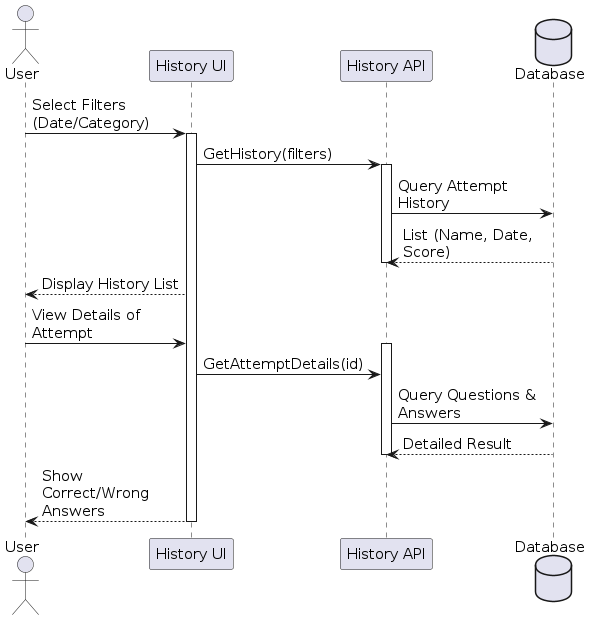
\includegraphics[width=\textwidth]{Image/Diagrams/Sequence/HistorySequence.png}
  \vspace{1.0cm}
  
  \caption{Sequence diagram - View Exercise History}
\end{figure}
\newpage
\begin{figure}[H]
  \centering
  \begin{adjustbox}{max height=0.9\textheight}
    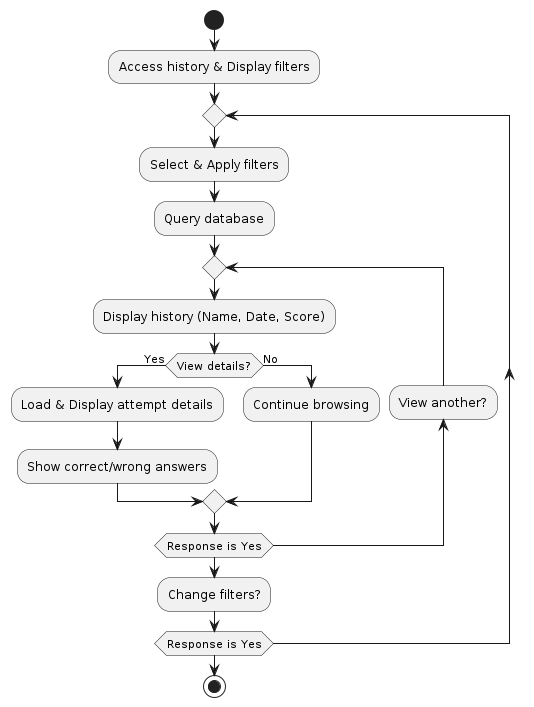
\includegraphics{Image/Diagrams/Activity/HistoryActivity.png}
  \end{adjustbox}
   \vspace{0.6cm}
  \caption{Activity diagram - View Exercise History}
\end{figure}
\newpage

\subsubsection{Chơi trò chơi (Play Minigames)}
\begin{table}[H]
\centering
\renewcommand{\arraystretch}{1.3}
\begin{tabular}{|l|p{0.75\textwidth}|}
\hline
\textbf{Usecase name} & Play Minigame \\
\hline
\textbf{Actor} & Student \\
\hline
\textbf{Description} & Cho phép Student chơi các minigame có sẵn trong hệ thống. \\
\hline
\textbf{Precondition} & Student đã đăng nhập vào hệ thống. \\
\hline
\textbf{Postcondition} & Student hoàn thành minigame và kết quả được lưu vào hệ thống. \\
\hline
\textbf{Main flow} & 
1. Student truy cập vào trang minigames. \newline
2. Hệ thống tải danh sách các minigame có sẵn. \newline
3. Hệ thống kiểm tra trạng thái premium của Student. \newline
4. Hệ thống hiển thị danh sách minigame (Free games + Premium games). \newline
5. Student chọn một minigame để chơi. \newline
6. Hệ thống kiểm tra quyền truy cập game. \newline
7. Hệ thống tải minigame. \newline
8. Hệ thống khởi động minigame. \newline
9. Student chơi minigame. \newline
10. Student hoàn thành và nộp kết quả minigame. \newline
11. Hệ thống lưu tiến trình và điểm số vào database. \newline
12. Hệ thống hiển thị kết quả hoàn thành/điểm số cho Student. \\
\hline
\textbf{Alternative flow} & 
\textit{Alternative flow 1: Student chọn chơi minigame khác} \newline
Tại bước 12: Student muốn chơi minigame khác. \newline
Student quay lại bước 4 để chọn minigame mới. \\
\hline
\textbf{Exception} & 
\textit{Exception 1: Không có quyền truy cập game premium} \newline
Tại bước 6: Hệ thống phát hiện Student không có quyền truy cập game premium. \newline
Hệ thống hiển thị thông báo "Yêu cầu Premium" với nút "Mua Premium". \newline
Usecase kết thúc. \newline\newline
\textit{Exception 2: Lỗi khi lưu kết quả} \newline
Tại bước 11: Hệ thống không thể lưu kết quả game. \newline
Hệ thống hiển thị thông báo lỗi. \newline
\\ \hline
\end{tabular}
\caption{Usecase - Play Minigame}
\label{table:uc_playminigame}
\end{table}

\newpage
\begin{figure}[H]
\centering
\begin{adjustbox}{max height=0.9\textheight}
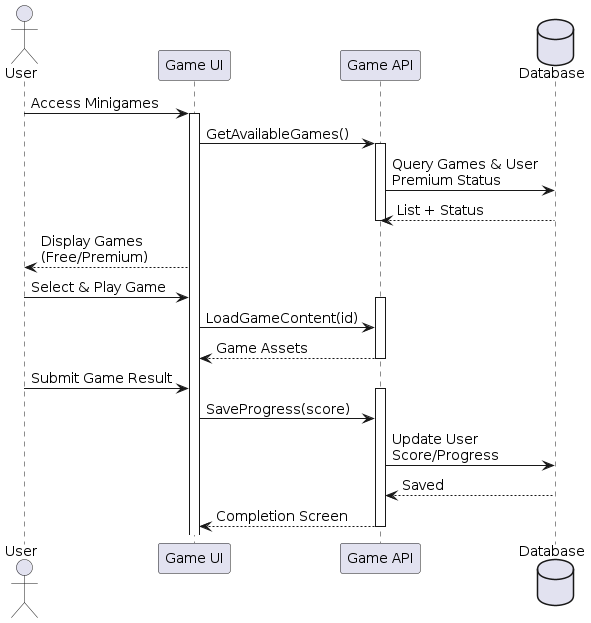
\includegraphics[width=0.8\textwidth]{Image/Diagrams/Sequence/GameSequence.png}
\end{adjustbox}
\vspace{1.0cm}
\caption{Sequence diagram - Play Minigame}
\end{figure}

\newpage
\begin{figure}[H]
\centering
\begin{adjustbox}{max height=0.9\textheight}
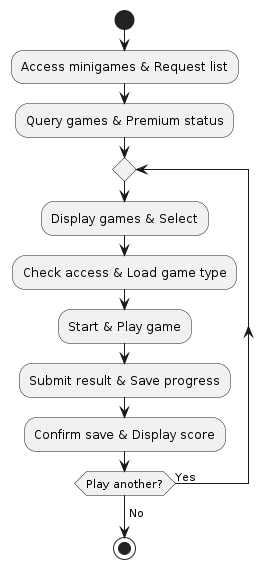
\includegraphics{Image/Diagrams/Activity/GameActivity.png}
\end{adjustbox}
\vspace{0.6cm}
\caption{Activity diagram - Play Minigame}
\end{figure}

\subsubsection{Xem thống kê của học sinh (View Student Statistics)}
\begin{table}[H]
\centering
\renewcommand{\arraystretch}{1.3}
\begin{tabular}{|l|p{0.75\textwidth}|}
\hline
\textbf{Usecase name} & View Student Statistics \\
\hline
\textbf{Actor} & Parent \\
\hline
\textbf{Description} & Cho phép Parent xem thống kê học tập và hoạt động của Student được liên kết. \\
\hline
\textbf{Precondition} & Parent đã đăng nhập vào hệ thống và có ít nhất một Student được liên kết. \\
\hline
\textbf{Postcondition} & Parent xem được thống kê chi tiết về hoạt động học tập và arena của Student. \\
\hline
\textbf{Main flow} & 
1. Parent truy cập vào trang thống kê. \newline
2. Hệ thống truy vấn danh sách Student liên kết với Parent. \newline
3. Hệ thống hiển thị dropdown chọn Student. \newline
4. Parent chọn một Student. \newline
5. Hệ thống truy vấn thống kê học tập (số bài tập đã làm, tỉ lệ làm đúng, số giờ hoạt động). \newline
6. Hệ thống truy vấn thống kê arena (xếp hạng, battle points, xếp hạng tuần, tỉ lệ làm đúng). \newline
7. Hệ thống truy vấn thành tích của Student (rank badge và tiến trình). \newline
8. Hệ thống hiển thị dashboard thống kê đầy đủ (Learning stats + Arena stats + Badge). \\
\hline
\textbf{Alternative flow} & 
\textit{Alternative flow 1: Áp dụng bộ lọc ngày tháng} \newline
Tại bước 8: Parent muốn xem thống kê theo khoảng thời gian cụ thể. \newline
Parent chọn khoảng ngày (From - To). \newline
Hệ thống truy vấn thống kê với bộ lọc ngày tháng. \newline
Hệ thống hiển thị kết quả thống kê đã lọc. \newline\newline
\textit{Alternative flow 2: Thay đổi Student} \newline
Tại bước 8: Parent muốn xem thống kê của Student khác. \newline
Parent chọn Student khác từ dropdown. \newline
Hệ thống quay lại bước 5 để tải thống kê của Student mới. \\
\hline
\textbf{Exception} & 
\textit{Exception 1: Khoảng ngày không hợp lệ} \newline
Tại Alternative flow 1: Hệ thống phát hiện khoảng ngày không hợp lệ. \newline
Hệ thống hiển thị thông báo lỗi "Invalid date range". \newline
Parent cần nhập lại khoảng ngày hợp lệ. \\
\hline
\end{tabular}
\caption{Usecase - View Student Statistics}
\label{table:uc_viewstudentstatistics}
\end{table}

\newpage
\begin{figure}[H]
\centering
\begin{adjustbox}{max height=0.9\textheight}
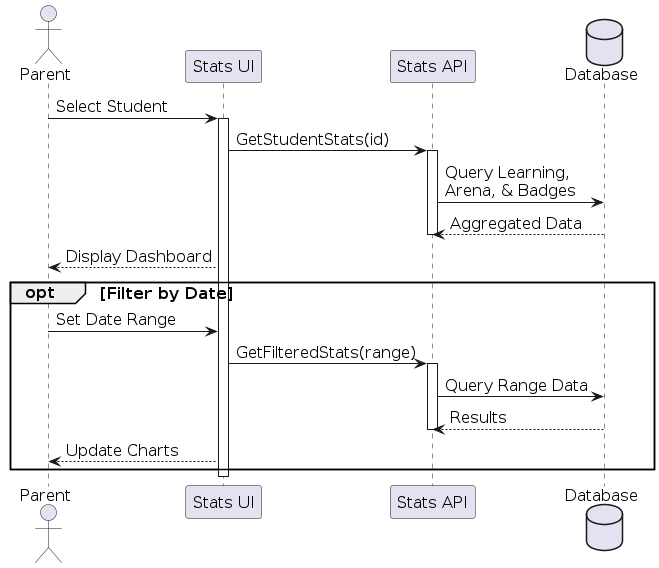
\includegraphics[width=0.8\textwidth]{Image/Diagrams/Sequence/StatsSequence.png}
\end{adjustbox}
\vspace{1.0cm}
\caption{Sequence diagram - View Student Statistics}
\end{figure}

\newpage
\begin{figure}[H]
\centering
\begin{adjustbox}{max height=0.9\textheight}
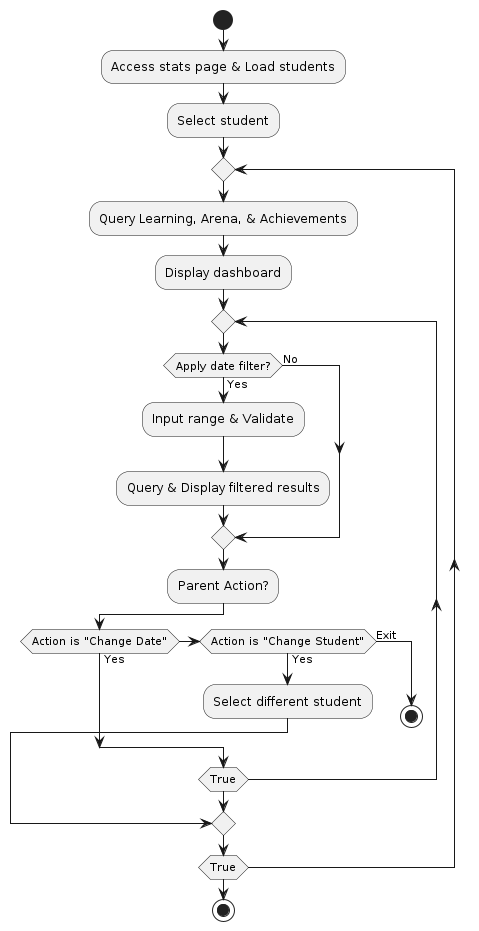
\includegraphics{Image/Diagrams/Activity/StatsActivity.png}
\end{adjustbox}
\vspace{0.6cm}
\caption{Activity diagram - View Student Statistics}
\end{figure}

\newpage
\subsubsection{Đăng ký gói Premium (Subscribe Premium)}
\begin{longtable}{|l|p{0.75\textwidth}|}
\caption{Usecase - Subscribe Premium}
\label{table:uc_subscribepremium} \\
\hline
\textbf{Usecase name} & Subscribe Premium \\
\hline
\textbf{Actor} & Parent \\
\hline
\textbf{Description} & Cho phép Parent nâng cấp tài khoản lên Premium để mở khóa toàn bộ tính năng cho Student. \\
\hline
\textbf{Precondition} & Parent đã đăng nhập vào hệ thống. \\
\hline
\textbf{Postcondition} & Parent nâng cấp thành công tài khoản Premium và tất cả tính năng được kích hoạt cho Student. \\
\hline
\textbf{Main flow} & 
1. Parent truy cập vào trang premium subscription. \newline
2. Hệ thống truy vấn các gói đăng ký có sẵn. \newline
3. Hệ thống truy vấn trạng thái đăng ký hiện tại của Parent. \newline
4. Hệ thống hiển thị các gói đăng ký (Free: 0đ vs Premium: 599,000đ). \newline
5. Parent chọn gói Premium. \newline
6. Hệ thống hiển thị các lợi ích của Premium (No time limit, No minigames limit, All features unlocked). \newline
7. Parent nhấn nút "Nâng cấp ngay". \newline
8. Hệ thống tạo đơn hàng đăng ký. \newline
9. Hệ thống khởi tạo phiên thanh toán. \newline
10. Hệ thống hiển thị các phương thức thanh toán (Bank transfer, QR code, E-wallet). \newline
11. Parent hoàn thành thanh toán. \newline
12. Payment Gateway gửi thông báo webhook về kết quả thanh toán. \newline
13. Hệ thống xác minh giao dịch thanh toán. \newline
14. Hệ thống cập nhật đăng ký Parent lên Premium. \newline
15. Hệ thống kích hoạt các tính năng premium (Unlock minigames, Remove time limits, Grant full access). \newline
16. Hệ thống cập nhật trạng thái đơn hàng thành "completed". \newline
17. Hệ thống gửi thông báo xác nhận cho Parent. \newline
18. Hệ thống hiển thị thông báo "Nâng cấp thành công!". \newline
19. Hệ thống chuyển hướng Parent về dashboard. \\
\hline
\textbf{Alternative flow} & 
\textit{Alternative flow 1: Parent xem trạng thái đăng ký hiện tại} \newline
Tại bước 4: Parent muốn xem thông tin đăng ký hiện tại. \newline
Parent nhấn "View current plan". \newline
Hệ thống truy vấn chi tiết đăng ký của Parent. \newline
Hệ thống hiển thị gói hiện tại và ngày hết hạn. \newline
Parent quay lại bước 4. \newline\newline
\textit{Alternative flow 2: Parent hủy thanh toán} \newline
Tại bước 11: Parent quyết định không thanh toán. \newline
Parent đóng trang thanh toán. \newline
Usecase kết thúc. \\
\hline
\textbf{Exception} &
\textit{Exception 1: Thanh toán thất bại} \newline
Tại bước 12: Payment Gateway thông báo thanh toán thất bại. \newline
Hệ thống cập nhật trạng thái đơn hàng thành "failed". \newline
Hệ thống hiển thị thông báo lỗi thanh toán với tùy chọn thử lại. \newline
Parent có thể quay lại bước 10 để thử lại thanh toán hoặc kết thúc usecase. \newline\newline
\textit{Exception 2: Lỗi xác minh giao dịch} \newline
Tại bước 13: Hệ thống không thể xác minh giao dịch. \newline
Hệ thống ghi log lỗi và thông báo cho admin. \newline
Hệ thống hiển thị thông báo "Đang xử lý, vui lòng chờ xác nhận". \newline
Usecase kết thúc. \\
\hline
\end{longtable}


\newpage
\begin{figure}[H]
\centering
\begin{adjustbox}{max height=0.9\textheight}
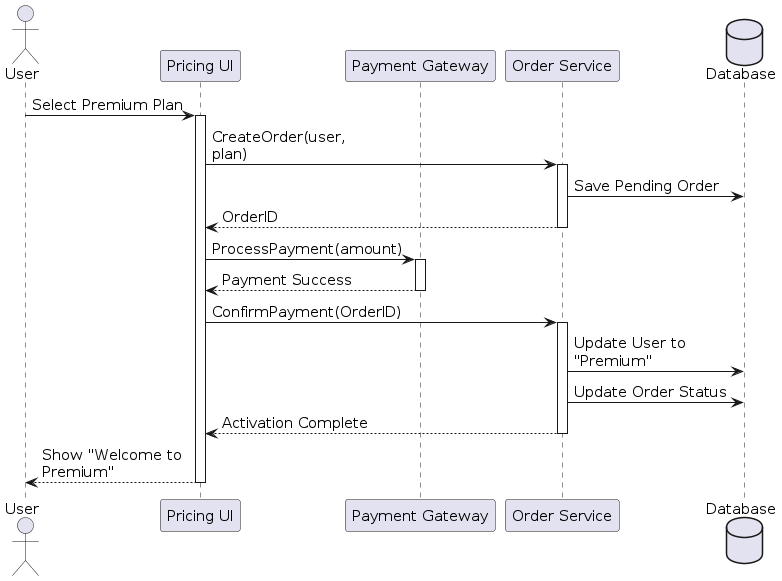
\includegraphics[width=0.9\textwidth]{Image/Diagrams/Sequence/PurchaseSequence.png}
\end{adjustbox}
\vspace{1.0cm}
\vspace{1.0em}
\caption{Sequence diagram - Subscribe Premium}
\end{figure}

\newpage
\begin{figure}[H]
\centering
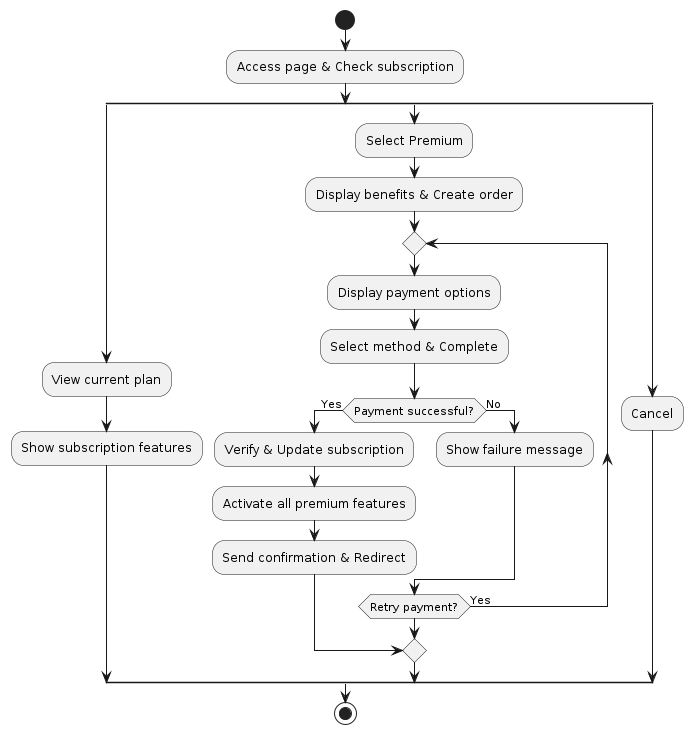
\includegraphics[width=0.9\textwidth]{Image/Diagrams/Activity/PurchaseActivity.png}
\vspace{0.6cm}
\caption{Activity diagram - Subscribe Premium}
\end{figure}

\newpage
\subsubsection{Quản lý bài học (Manage Lesson)}
\begin{longtable}{|l|p{0.75\textwidth}|}
	\caption{Usecase - Manage Lesson}
	\label{table:uc_managelesson} \\
	\hline
	\textbf{Usecase name} & Manage Lesson\\
	\hline
	\endfirsthead
	\hline
	\textbf{Usecase name} & Manage Lesson (tiếp) \\
	\hline
	\endhead
	\hline
	\textbf{Actor} & Admin \\
	\hline
	\textbf{Description} & Cho phép Admin quản lý chi tiết một bài học cụ thể, bao gồm việc thêm mới bài học (thủ công/Excel), chỉnh sửa nội dung lý thuyết bằng HTML và quản lý danh sách bài tập bằng giao diện Form hoặc mã nguồn JSON. \\
	\hline
	\textbf{Precondition} & Admin đã truy cập vào giao diện Quản lý bài học. \\
	\hline
	\textbf{Postcondition} & Các thay đổi về nội dung lý thuyết và bài tập được lưu trữ thành công vào hệ thống. \\
	\hline
	\textbf{Main flow} &
	1. Admin chọn phương thức khởi tạo bài học: nhập Form thủ công hoặc tải tệp Excel. \newline
	2. Hệ thống hiển thị giao diện chi tiết bài học sau khi khởi tạo thành công. \newline
	3. Admin truy cập tab "Quản lý lý thuyết" để chỉnh sửa các khối nội dung HTML. \newline
	4. Admin truy cập tab "Quản lý bài tập" để thêm, sửa hoặc xóa các câu hỏi. \newline
	5. Hệ thống thực hiện kiểm tra tính hợp lệ của dữ liệu (Validation) và cú pháp (JSON/HTML). \newline
	6. Admin nhấn "Lưu thay đổi". \newline
	7. Hệ thống hiển thị thông báo thành công và cập nhật lại trạng thái bài học. \\
	\hline
	\textbf{Alternative flow} &
	\textit{Alternative flow 1: Import bài tập/bài học từ Excel} \newline
	Tại bước 1: Admin chọn "Import Excel" và tải tệp lên. \newline
	Hệ thống kiểm tra cấu trúc tệp; nếu hợp lệ, dữ liệu sẽ được đổ vào các trường tương ứng. \newline\newline
	\textit{Alternative flow 2: Quản lý bài tập bằng JSON} \newline
	Tại bước 4: Admin chuyển đổi chế độ nhập liệu từ Form sang "JSON Editor". \newline
	Admin chỉnh sửa trực tiếp mã JSON của danh sách bài tập. \newline
	Hệ thống kiểm tra lỗi cú pháp JSON thời gian thực. \newline\newline
	\textit{Alternative flow 3: Preview nội dung} \newline
	Tại bất kỳ bước nào trước khi lưu: Admin nhấn nút "Preview". \newline
	Hệ thống hiển thị giao diện bài học thực tế (Live View) như cách học sinh sẽ nhìn thấy. \newline\newline
	\textit{Alternative flow 4: Xuất tệp mẫu (Export Sample)} \newline
	Tại giao diện quản lý: Admin nhấn "Tải tệp mẫu". \newline
	Hệ thống tạo và tải xuống tệp Excel trống có sẵn định dạng cột chuẩn. \\
	\hline
	\textbf{Exception} &
	\textit{Exception 1: Lỗi cú pháp mã nguồn (JSON/HTML)} \newline
	Tại bước 5: Hệ thống phát hiện lỗi cú pháp trong trình chỉnh sửa. \newline
	Hệ thống đánh dấu đỏ vị trí lỗi và vô hiệu hóa nút "Lưu". \newline\newline
	\textit{Exception 2: Tệp Excel không hợp lệ} \newline
	Tại AF1: Tệp tải lên sai định dạng hoặc chứa dữ liệu rác. \newline
	Hệ thống từ chối nhập liệu. \newline\newline
	\textit{Exception 3: Trùng lặp mã bài học} \newline
	Tại bước 6: Admin lưu bài học với mã định danh đã tồn tại. \newline
	Hệ thống báo lỗi "Mã bài học đã tồn tại" và yêu cầu nhập lại. \\
	\hline
\end{longtable}

\newpage
\begin{figure}[H]
\centering
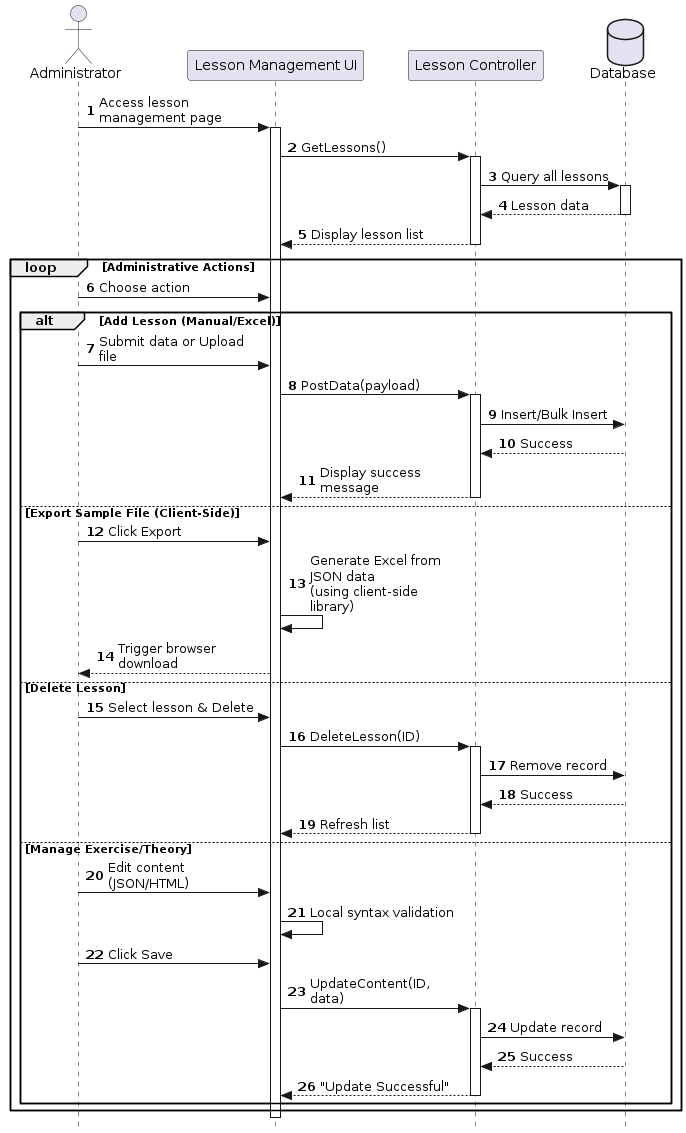
\includegraphics[width=0.9\textwidth]{Image/Diagrams/Sequence/AdminSequence.png}
\vspace{0.5cm}
\caption{Sequence diagram - Manage Lesson}
\end{figure}

\newpage
\begin{figure}[H]
\centering
\begin{adjustbox}{max width=\textwidth, max height=0.9\textheight}
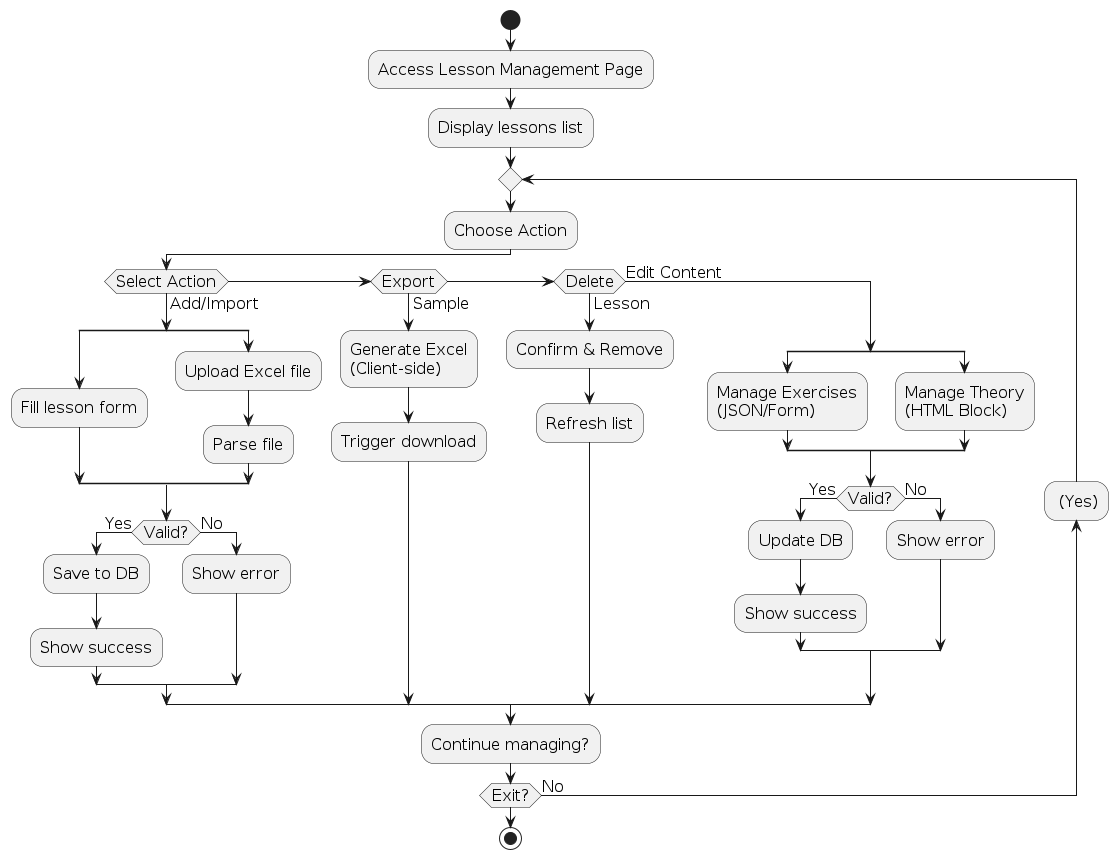
\includegraphics{Image/Diagrams/Activity/AdminActivity.png}
\end{adjustbox}
\vspace{0.6cm}
\caption{Activity diagram - Manage Lesson}
\end{figure}

\newpage
\subsection{Mô tả kiến trúc hệ thống}
\begin{figure}[h!]
	\centering
	\setlength{\abovecaptionskip}{10pt}
	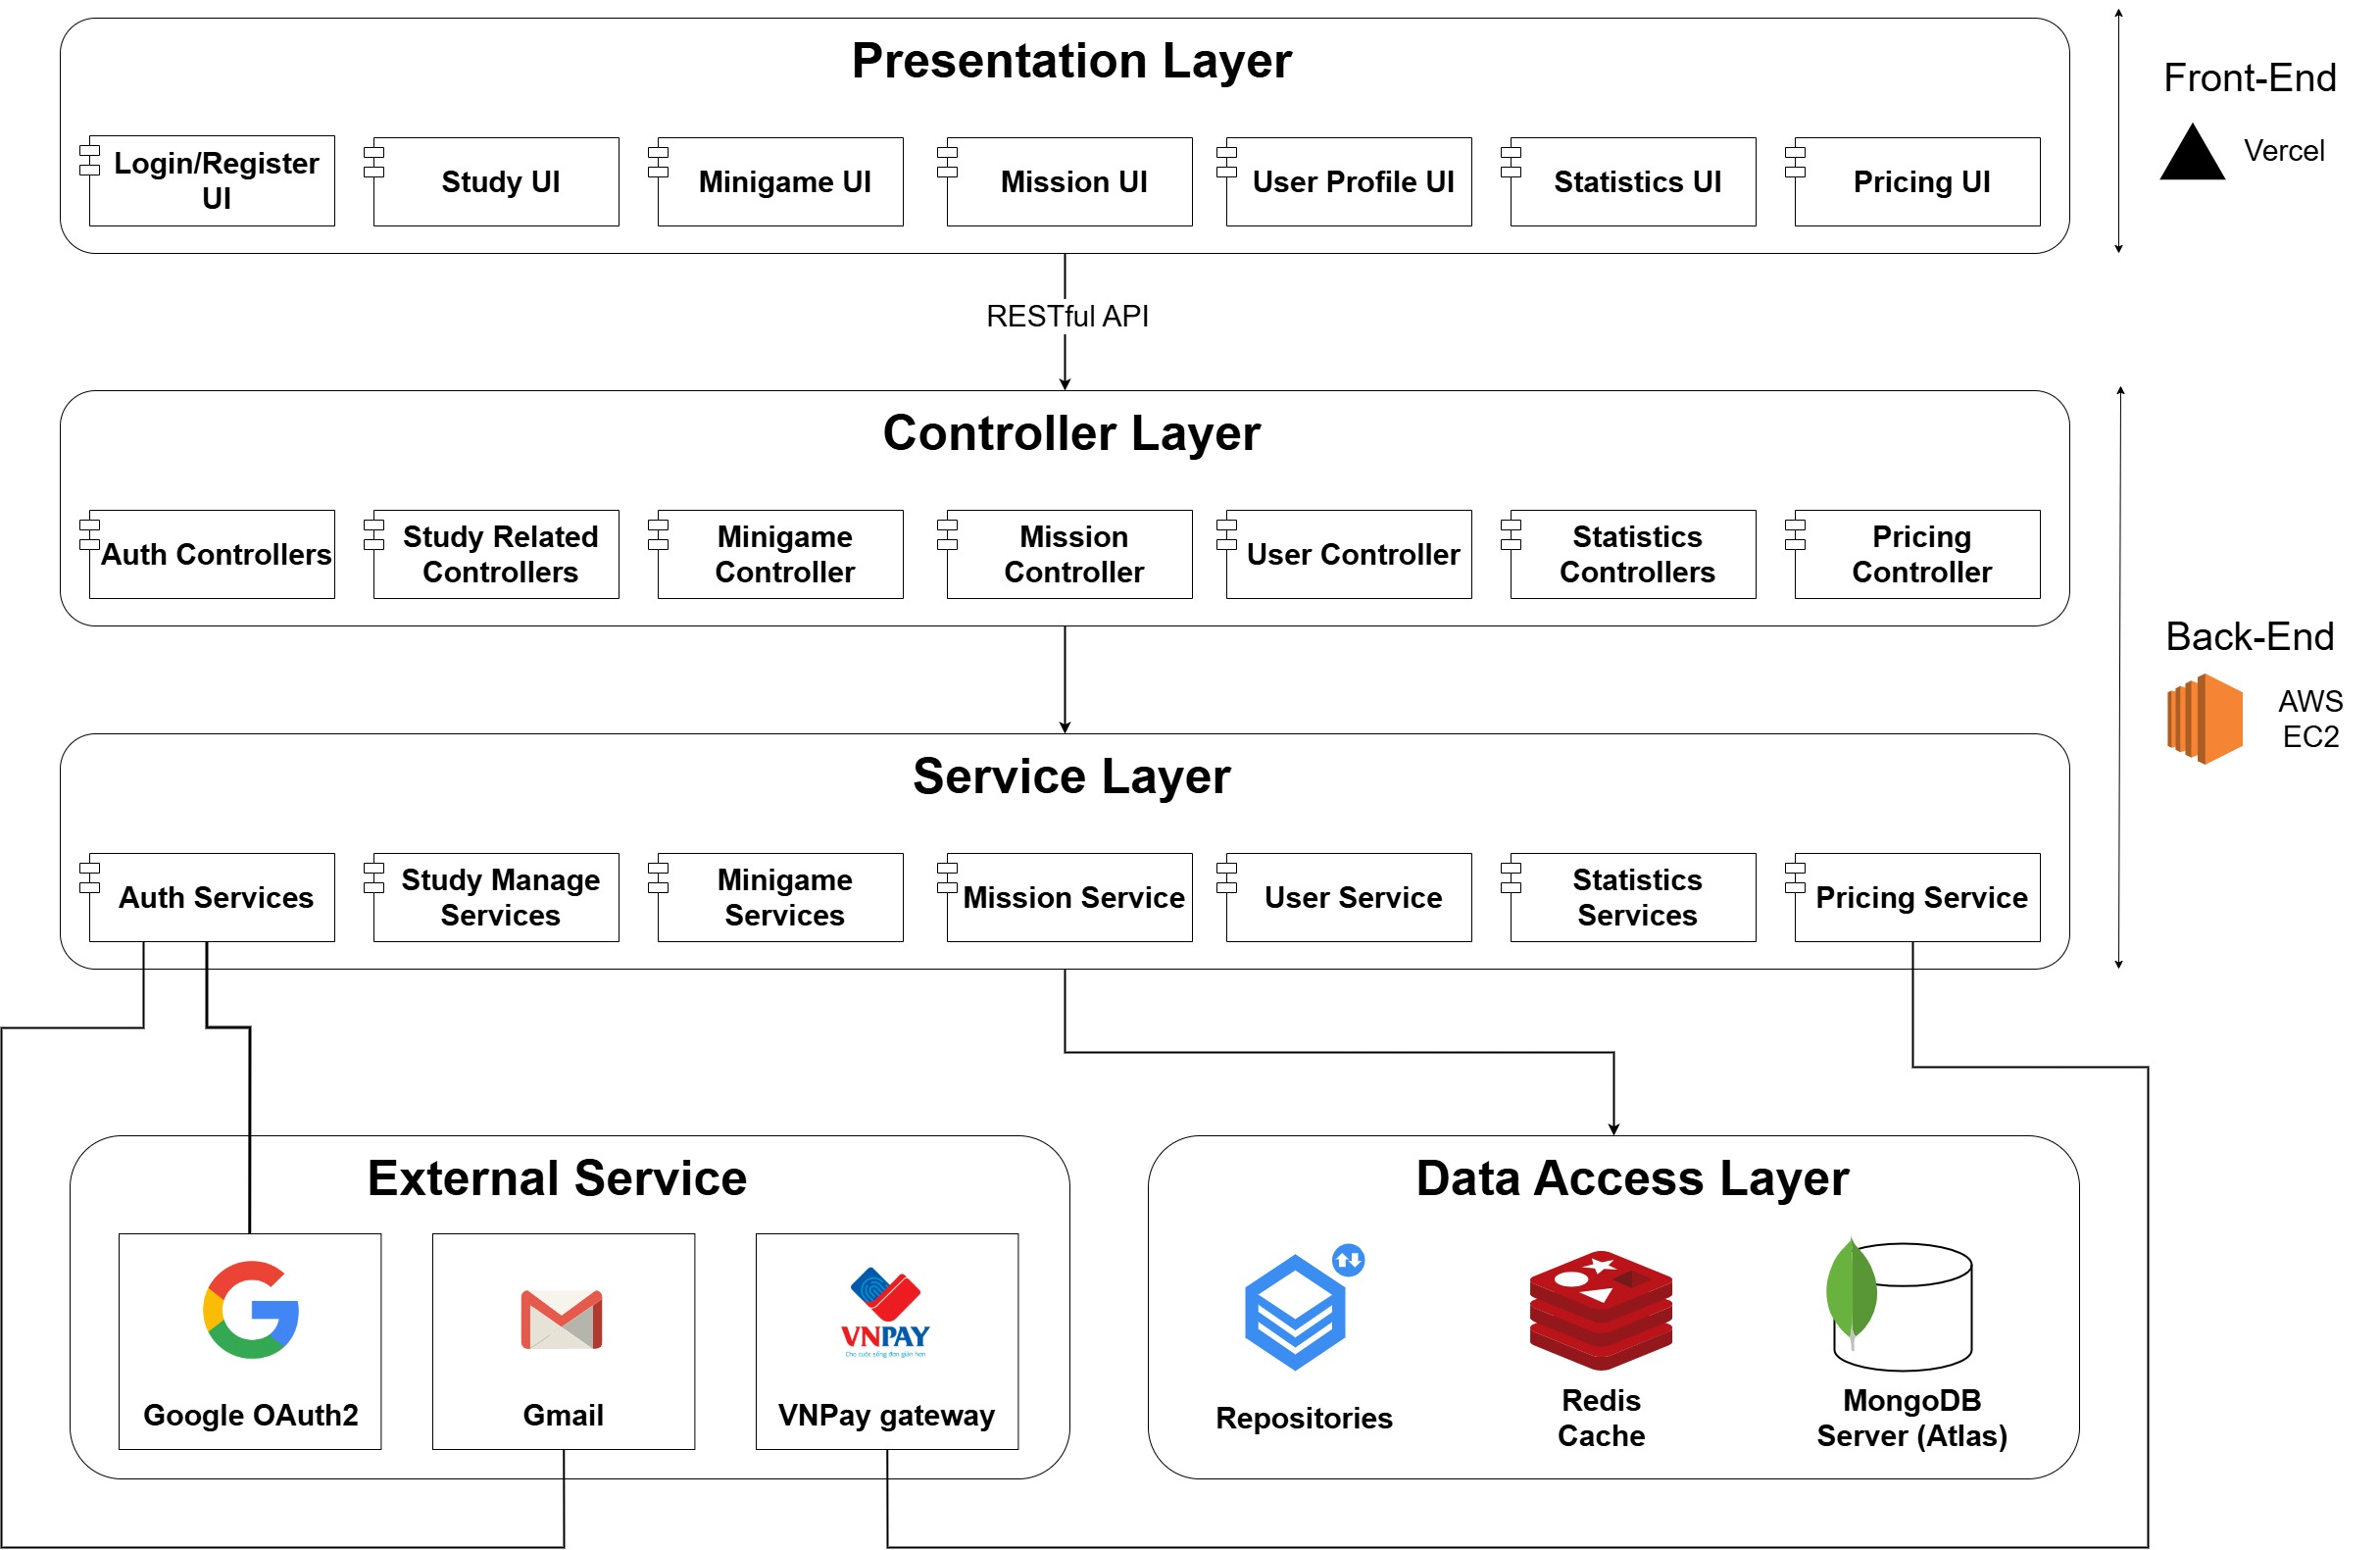
\includegraphics[width=\textwidth]{Image/Architecture.jpg}
	\caption{Sơ đồ kiến trúc tổng thể của hệ thống}
	\label{fig:system-architecture}
\end{figure}


Hệ thống được thiết kế theo mô hình kiến trúc nhiều tầng (layered architecture), nhằm tách biệt rõ ràng giữa giao diện người dùng, xử lý nghiệp vụ và truy cập dữ liệu, từ đó tăng khả năng mở rộng, bảo trì và kiểm thử.
Hệ thống được thiết kế theo mô hình kiến trúc nhiều tầng (layered architecture), nhằm tách biệt rõ ràng giữa giao diện người dùng, xử lý nghiệp vụ và truy cập dữ liệu, từ đó tăng khả năng mở rộng, bảo trì và kiểm thử.

\subsubsection{Tầng Trình bày (Presentation Layer)}
Tầng trình bày chịu trách nhiệm tương tác trực tiếp với người dùng, bao gồm các giao diện và chức năng như:
\begin{itemize}
	\item \textit{Đăng nhập/Đăng ký} (Login/Register UI)
	\item Các giao diện liên quan đến học tập: Chủ đề, Đấu trường, Bài kiểm tra, Bài tập tương tác được thể hiện chung trên sơ đồ \textit{Hình \ref{fig:system-architecture} } qua component Study UI.
	\item \textit{Nhiệm vụ} (Mission UI)
	\item \textit{Hồ sơ người dùng} (User Profile UI)
	\item \textit{Trò chơi} (Minigame UI)
	\item \textit{Thống kê} (Statistics UI): bao gồm các giao diện lịch sử, bảng xếp hạng, các thông số học tập,...
\end{itemize}

Các thành phần thuộc tầng này không xử lý logic nghiệp vụ, mà chỉ có nhiệm vụ gửi yêu cầu (request) đến Tầng Điều khiển và hiển thị kết quả (response) trả về cho người dùng.

\subsubsection{Tầng Điều khiển (Controller Layer)}
Tầng điều khiển đóng vai trò trung gian giữa Tầng Trình bày và Tầng Dịch vụ (Service Layer).  

Mỗi bộ điều khiển (Controller) như: \textit{Xác thực} (Auth), \textit{Trò chơi} (Minigame), \textit{Nhiệm vụ} (Mission), \textit{Học tập} (Study), \textit{Thống kê} (Statistics),... tiếp nhận yêu cầu từ giao diện người dùng, điều phối luồng xử lý và gọi các thành phần nghiệp vụ tương ứng.  

\subsubsection{Tầng Dịch vụ (Service Layer)}
Tầng Dịch vụ chứa các dịch vụ cốt lõi (Core Services) của hệ thống, bao gồm \textit{Dịch vụ Xác thực} (Auth Service), \textit{Dịch vụ Trò chơi} (Minigame Service), \textit{Các dịch vụ liên quan đến học tập} (Study Services), \textit{Dịch vụ Nhiệm vụ} (Mission Service), \textit{Dịch vụ quản lý người dùng} (User Service), \textit{Các dịch vụ Thống kê} (Statistics Services), \textit{Các dịch vụ liên quan đến gói trả phí và thanh toán} (Pricing Services).  

Mỗi dịch vụ chịu trách nhiệm xử lý một nhóm nghiệp vụ cụ thể, đóng gói các quy tắc nghiệp vụ và đảm bảo tính nhất quán của dữ liệu.  
Các dịch vụ có thể giao tiếp với nhau khi cần thiết, đồng thời tương tác với các dịch vụ bên ngoài.

\subsubsection{Tầng Truy cập Dữ liệu (Data Access Layer)}
Tầng truy cập dữ liệu chịu trách nhiệm lưu trữ và truy xuất dữ liệu từ hệ quản trị cơ sở dữ liệu MongoDB.  

Mọi thao tác liên quan đến dữ liệu đều được thực hiện thông qua tầng này, giúp cô lập logic nghiệp vụ khỏi chi tiết cài đặt của hệ quản trị cơ sở dữ liệu.

\subsubsection{Các Dịch vụ Bên ngoài (External Services)}
Hệ thống tích hợp với các dịch vụ bên ngoài như \textit{Cổng thanh toán} (Payment Gateway) để xử lý giao dịch, \textit{Dịch vụ Email} (Email Service) để gửi thông báo, dịch vụ xác thực người dùng thông qua tài khoản Google.  

Việc tách riêng các dịch vụ bên ngoài giúp hệ thống dễ dàng thay thế, mở rộng hoặc nâng cấp trong tương lai mà không ảnh hưởng đến các thành phần cốt lõi.

\subsubsection{Luồng Xử lý Tổng quát}
Người dùng tương tác với Tầng Trình bày, các yêu cầu được chuyển đến bộ điều khiển (Controller) tương ứng.  
Sau khi dữ liệu được xác thực và kiểm tra hợp lệ, yêu cầu sẽ được xử lý tại Tầng Dịch vụ thông qua các dịch vụ phù hợp, đồng thời truy xuất hoặc cập nhật dữ liệu tại Tầng Truy cập Dữ liệu.  
Cuối cùng, kết quả xử lý được trả về Tầng Trình bày để hiển thị cho người dùng.

\subsection{Thiết kế cơ sở dữ liệu}
Phần này trình bày chi tiết các thực thể chính trong hệ thống Dino Math, bao gồm vai trò, đặc điểm và mối quan hệ giữa chúng. Các thực thể được thiết kế nhằm đáp ứng đồng thời hai mục tiêu cốt lõi:
\begin{enumerate}
	\item Quản lý hiệu quả quá trình học tập của người dùng.
	\item Tích hợp các yếu tố trò chơi hóa để nâng cao mức độ tương tác và hứng thú học tập.
\end{enumerate}
\begin{figure}[H]
	\centering
	\includegraphics[width=\textwidth]{Image/ERD.jpg}
	\vspace{0.5cm}
	
	\caption{Sơ đồ thực thể – quan hệ (ERD) của hệ thống}
	\label{fig:erd-diagram}
\end{figure}

Dựa trên sơ đồ thực thể – quan hệ (ERD) ở Hình~\ref{fig:erd-diagram}, hệ thống được chia thành các thực thể chính sau đây.

\subsubsection{Quản lý Người dùng và Gia đình (User \& Family)}

Đây là nhóm thực thể nền tảng, đóng vai trò trung tâm trong việc quản lý tài khoản, phân quyền truy cập và mối quan hệ giữa các người dùng trong hệ thống.

\subsubsubsection{User (Người dùng)}

\texttt{User} là thực thể trung tâm của hệ thống, đại diện cho tất cả các đối tượng sử dụng ứng dụng, bao gồm học sinh, phụ huynh và quản trị viên. 
Mỗi người dùng được phân loại thông qua thuộc tính \texttt{role} và được kiểm soát trạng thái hoạt động thông qua \texttt{status}.

\newline
\vspace{0.2cm}
Thực thể \texttt{User} lưu trữ các thông tin cá nhân cơ bản như tên, email, mật khẩu (đã được mã hóa), ảnh đại diện và các thiết lập cá nhân hóa trải nghiệm (ngôn ngữ, thông báo, v.v.). 
Bên cạnh đó, \texttt{User} còn giữ vai trò liên kết tới hầu hết các chức năng nghiệp vụ quan trọng trong hệ thống.

\begin{table}[H]
	\centering
	\begin{tabularx}{\textwidth}{|l|l|X|}
		\hline
		\textbf{Thuộc tính} & \textbf{Kiểu dữ liệu} & \textbf{Mô tả} \\ \hline
		\_id & ObjectId & Khóa chính định danh người dùng. \\ \hline
		name & String & Họ và tên hiển thị. \\ \hline
		username & String & Tên đăng nhập. \\ \hline
		email & String & Địa chỉ email liên kết tài khoản. \\ \hline
		password & String & Mật khẩu (đã được mã hóa). \\ \hline
		role & Enum & Vai trò: \texttt{student}, \texttt{parent}, \texttt{admin}. \\ \hline
		status & Enum & Trạng thái: \texttt{active}, \texttt{inactive}, \texttt{pending\_profile}. \\ \hline
		familyId & ObjectId & Tham chiếu đến gia đình (Family). \\ \hline
		gradeId & ObjectId & Tham chiếu đến khối lớp (Grade). \\ \hline
		quartz & Number & Số lượng đá quý hiện có. \\ \hline
		battlePoints & Number & Điểm thi đấu tích lũy. \\ \hline
		rankId & ObjectId & Tham chiếu đến cấp bậc (Rank). \\ \hline
	\end{tabularx}
	\caption{Các thuộc tính chính của thực thể User}
\end{table}
\newline
\textbf{Các mối quan hệ chính của User:}
\begin{itemize}
	\item Thuộc về một \texttt{Family}, cho phép liên kết giữa phụ huynh và học sinh.
	\item Được gán vào một \texttt{Grade} để xác định chương trình học phù hợp.
	\item Liên kết với một \texttt{Rank} nhằm phản ánh cấp bậc và tiến trình của người dùng trong hệ thống.
	\item Có nhiều bản ghi \texttt{Progress} để theo dõi tiến độ học tập.
	\item Tham gia các bài giảng và bài kiểm tra, sinh ra các thực thể \texttt{LectureResult}, \texttt{ExerciseResult} và \texttt{AssessmentResult}.
	\item Tham gia các hoạt động thi đấu thông qua \texttt{Participation} trong các \texttt{Arena}.
	\item Nhận phần thưởng và thành tựu thông qua các thực thể \texttt{Achievement} và \texttt{RewardRecord}.
\end{itemize}

\subsubsubsection{Family (Gia đình)}
\texttt{Family} đại diện cho một nhóm người dùng có mối quan hệ gia đình, cho phép phụ huynh quản lý và theo dõi quá trình học tập của học sinh. 
Mỗi gia đình được tạo ra với một mã mời (\texttt{inviteCode}), cho phép các thành viên mới tham gia một cách thuận tiện.

\begin{table}[H]
	\centering
	\begin{tabularx}{\textwidth}{|l|l|X|}
		\hline
		\textbf{Thuộc tính} & \textbf{Kiểu dữ liệu} & \textbf{Mô tả} \\ \hline
		\_id & ObjectId & Khóa chính định danh gia đình. \\ \hline
		name & String & Tên nhóm gia đình. \\ \hline
		inviteCode & String & Mã mời thành viên mới. \\ \hline
		inviteSingleUse & Boolean & Xác định mã mời dùng một lần hay nhiều lần. \\ \hline
	\end{tabularx}
	\caption{Các thuộc tính chính của thực thể Family}
\end{table}

\newline
\textbf{Các mối quan hệ chính của Family:}
\begin{itemize}
	\item Chứa nhiều thành viên \texttt{User}.
	\item Liên kết với các báo cáo học tập tổng hợp thông qua \texttt{FamilyReport}.
	\item Tổ chức các hoạt động tương tác thông qua các \texttt{FamilyGame}.
\end{itemize}

\subsubsection{Cấu trúc Chương trình Học (Academic \& Structure)}
Nhóm thực thể này chịu trách nhiệm tổ chức nội dung học tập theo chương trình giáo dục, đồng thời hỗ trợ hiển thị và điều hướng nội dung một cách trực quan trong hệ thống.

\subsubsubsection{Grade (Khối lớp)}

\texttt{Grade} đại diện cho một cấp độ học tập cụ thể (ví dụ: Lớp 1, Lớp 2). 
Mỗi khối lớp được liên kết với một \texttt{World} riêng biệt, giúp xây dựng chủ đề và giao diện học tập phù hợp với từng độ tuổi.

\begin{table}[H]
	\centering
	\begin{tabularx}{\textwidth}{|l|l|X|}
		\hline
		\textbf{Thuộc tính} & \textbf{Kiểu dữ liệu} & \textbf{Mô tả} \\ \hline
		\_id & ObjectId & Khóa chính định danh khối lớp. \\ \hline
		name & String & Tên khối lớp (ví dụ: Lớp 1). \\ \hline
		level & Number & Cấp độ số của khối lớp. \\ \hline
		worldId & ObjectId & Tham chiếu đến thế giới (World) tương ứng. \\ \hline
	\end{tabularx}
	\caption{Các thuộc tính chính của thực thể Grade}
\end{table}

\newline
\textbf{Các mối quan hệ chính của Grade:}
\begin{itemize}
	\item Liên kết một--một với \texttt{World}.
	\item Chứa nhiều \texttt{Topic} thuộc chương trình học của khối lớp.
	\item Có nhiều \texttt{User} đang theo học.
	\item Liên quan đến các bài kiểm tra \texttt{Assessment}.
\end{itemize}

\subsubsubsection{AcademicTerm (Học kỳ)}
\texttt{AcademicTerm} được sử dụng để phân chia chương trình học theo từng giai đoạn thời gian như Học kỳ I, Học kỳ II hoặc Học kỳ hè. 
Thực thể này giúp hệ thống hiển thị và quản lý nội dung học tập phù hợp với mốc thời gian thực tế.
\begin{table}[H]
	\centering
	\begin{tabularx}{\textwidth}{|l|l|X|}
		\hline
		\textbf{Thuộc tính} & \textbf{Kiểu dữ liệu} & \textbf{Mô tả} \\ \hline
		\_id & ObjectId & Khóa chính định danh học kỳ (PK). \\ \hline
		name & String & Tên học kỳ (ví dụ: Semester 1, Semester 2, Summer,...). \\ \hline
		year & Number & Năm học tương ứng. \\ \hline
		term & Enum & Phân loại học kỳ (\texttt{semester1}, \texttt{semester2}, \texttt{summer}, \texttt{custom}). \\ \hline
		startDate & Date & Ngày bắt đầu học kỳ. \\ \hline
		endDate & Date & Ngày kết thúc học kỳ. \\ \hline
		isActive & Boolean & Trạng thái kích hoạt (xác định học kỳ hiện tại). \\ \hline
		notes & String & Ghi chú bổ sung về học kỳ. \\ \hline
	\end{tabularx}
	\caption{Các thuộc tính chính của thực thể AcademicTerm}
\end{table}
\newline
\textbf{Các mối quan hệ chính của AcademicTerm:}
\begin{itemize}
	\item Chứa nhiều \texttt{Topic} thuộc học kỳ tương ứng.
\end{itemize}

\subsubsubsection{Topic (Chủ đề)}
\texttt{Topic} là đơn vị kiến thức lớn trong chương trình học của một khối lớp. 
Mỗi chủ đề bao gồm thông tin mô tả, danh sách tuần học và được sử dụng để xây dựng lộ trình học tập chi tiết cho người dùng.
\begin{table}[H]
	\centering
	\begin{tabularx}{\textwidth}{|l|l|X|}
		\hline
		\textbf{Thuộc tính} & \textbf{Kiểu dữ liệu} & \textbf{Mô tả} \\ \hline
		\_id & ObjectId & Khóa chính (PK). \\ \hline
		title & String & Tiêu đề chủ đề. \\ \hline
		description & String & URL ảnh chủ đề. \\ \hline
		level & Number & Cấp độ/thứ tự của chủ đề. \\ \hline
		gradeId & String & Tham chiếu đến Grade (ref). \\ \hline
		termId & String & Tham chiếu đến AcademicTerm (ref). \\ \hline
		weekNumbers & [Number] & Các tuần học thuộc chủ đề này. \\ \hline
		isPremium & Boolean & Xác định chủ đề trả phí. \\ \hline
	\end{tabularx}
	\caption{Các thuộc tính chính của thực thể Topic}
\end{table}
\newline
\textbf{Các mối quan hệ chính của Topic:}
\begin{itemize}
	\item Thuộc về một \texttt{Grade}.
	\item Thuộc về một \texttt{AcademicTerm}.
	\item Chứa nhiều \texttt{Lecture}.
	\item Được theo dõi tiến độ thông qua \texttt{Progress}.
	\item Được tham chiếu trong các gợi ý học tập (\texttt{Recommendation}).
\end{itemize}

\subsubsubsection{Lecture (Bài giảng)}
\texttt{Lecture} đại diện cho một bài học cụ thể trong một chủ đề. 
Mỗi bài giảng có loại nội dung và độ khó riêng, giúp phân loại và điều chỉnh mức độ thử thách cho học sinh.
\begin{table}[H]
	\centering
	\begin{tabularx}{\textwidth}{|l|l|X|}
		\hline
		\textbf{Thuộc tính} & \textbf{Kiểu dữ liệu} & \textbf{Mô tả} \\ \hline
		\_id & ObjectId & Khóa chính (PK). \\ \hline
		title & String & Tiêu đề bài giảng. \\ \hline
		contentType & Enum & Loại nội dung (knowledge, understanding,...). \\ \hline
		description & String & Mô tả bài giảng. \\ \hline
		topicId & String & Tham chiếu đến Topic (ref). \\ \hline
		difficulty & Enum & Độ khó (easy, medium, hard). \\ \hline
		status & Enum & Trạng thái bài giảng (active, inactive). \\ \hline
		theory.content & String & Nội dung lý thuyết dạng văn bản/HTML. \\ \hline
		theory.videoUrl & String & Đường dẫn video bài giảng. \\ \hline
		theory.imageUrls & [String] & Danh sách hình ảnh minh họa lý thuyết. \\ \hline
	\end{tabularx}
	\caption{Các thuộc tính chính của thực thể Lecture}
\end{table}
\newline
\textbf{Các mối quan hệ chính của Lecture:}
\begin{itemize}
	\item Thuộc về một \texttt{Topic}.
	\item Chứa nhiều \texttt{Exercise}.
	\item Sinh ra các bản ghi kết quả học tập \texttt{LectureResult}.
\end{itemize}

\subsubsubsection{Exercise (Bài tập)}
\texttt{Exercise} là đơn vị nội dung nhỏ nhất trong hệ thống học tập, bao gồm các câu hỏi và hoạt động tương tác đa dạng như trắc nghiệm, đúng/sai, điền từ và kéo--thả.
\begin{table}[H]
	\centering
	\begin{tabularx}{\textwidth}{|l|l|X|}
		\hline
		\textbf{Thuộc tính} & \textbf{Kiểu dữ liệu} & \textbf{Mô tả} \\ \hline
		\_id & ObjectId & Khóa chính (PK). \\ \hline
		question & String & Nội dung câu hỏi. \\ \hline
		category & Enum & Phân loại (assessment, arena, lecture). \\ \hline
		type & Enum & Loại hình bài tập (matching, choice, fill\_in,...). \\ \hline
		options & [String] & Các tùy chọn trả lời. \\ \hline
		pairs & [Object] & Các cặp ghép nối (nếu là loại matching). \\ \hline
		correctAnswer & String & Đáp án chính xác. \\ \hline
		content & String & Nội dung bổ sung cho bài tập. \\ \hline
		metadata & Mixed & Dữ liệu mở rộng tùy biến. \\ \hline
		difficulty & Enum & Độ khó (easy, medium, hard). \\ \hline
		lectureId & Mixed & Tham chiếu đến Lecture (ref). \\ \hline
		arenaId & Mixed & Tham chiếu đến Arena (ref). \\ \hline
		assessmentId & Mixed & Tham chiếu đến Assessment (ref). \\ \hline
		order & Number & Thứ tự bài tập trong danh sách. \\ \hline
		explanation & String & Giải thích cho đáp án đúng. \\ \hline
	\end{tabularx}
	\caption{Các thuộc tính chính của thực thể Exercise}
\end{table}
\newline
\textbf{Các mối quan hệ chính của Exercise:}
\begin{itemize}
	\item Có thể thuộc về một \texttt{Lecture}.
	\item Được sử dụng trong các \texttt{Assessment} và \texttt{Arena}.
	\item Sinh ra các kết quả chi tiết thông qua \texttt{ExerciseResult} và \texttt{Answer}.
\end{itemize}

\subsubsection{Trò chơi hóa và Tài nguyên (Gamification \& Assets)}

Nhóm thực thể này đóng vai trò quan trọng trong việc tích hợp yếu tố trò chơi hóa vào quá trình học tập, nhằm tăng cường động lực và mức độ gắn kết của người dùng.

\subsubsubsection{World (Thế giới)}
\texttt{World} đại diện cho bối cảnh tổng thể của một khối lớp trong trò chơi. 
Mỗi thế giới được thiết kế phù hợp với độ tuổi và chủ đề học tập của khối lớp tương ứng.
\begin{table}[H]
	\centering
	\begin{tabularx}{\textwidth}{|l|l|X|}
		\hline
		\textbf{Thuộc tính} & \textbf{Kiểu dữ liệu} & \textbf{Mô tả} \\ \hline
		\_id & ObjectId & Khóa chính (PK). \\ \hline
		name & String & Tên thế giới chủ đề. \\ \hline
		milestoneUrl & String & Hình ảnh các mốc tiến trình. \\ \hline
	\end{tabularx}
	\caption{Các thuộc tính chính của thực thể World}
\end{table}
\newline
\textbf{Mối quan hệ:}
\begin{itemize}
	\item Liên kết một--một với \texttt{Grade}.
	\item Chứa nhiều \texttt{Land}.
\end{itemize}

\subsubsubsection{Land (Vùng đất)}
\texttt{Land} là các khu vực nhỏ trong một \texttt{World}, đại diện cho các nhóm bài học hoặc mức độ thử thách khác nhau.
\begin{table}[H]
	\centering
	\begin{tabularx}{\textwidth}{|l|l|X|}
		\hline
		\textbf{Thuộc tính} & \textbf{Kiểu dữ liệu} & \textbf{Mô tả} \\ \hline
		\_id & ObjectId & Khóa chính định danh vùng đất (PK). \\ \hline
		worldId & String & Tham chiếu đến thế giới (\texttt{World}) chứa vùng đất này. \\ \hline
		name & String & Tên vùng đất. \\ \hline
		difficulty & Enum & Mức độ thử thách (\texttt{easy}, \texttt{medium}, \texttt{hard}). \\ \hline
		imageUrl & String & Đường dẫn hình ảnh minh họa của vùng đất. \\ \hline
	\end{tabularx}
	\caption{Các thuộc tính chính của thực thể Land}
\end{table}
\newline
\textbf{Mối quan hệ:}
\begin{itemize}
	\item Thuộc về một \texttt{World}.
\end{itemize}

\subsubsubsection{Rank (Xếp hạng)}
\texttt{Rank} xác định cấp bậc của người dùng dựa trên điểm tích lũy từ các hoạt động học tập và thi đấu trong Đấu trường.
\begin{table}[H]
	\centering
	\begin{tabularx}{\textwidth}{|l|l|X|}
		\hline
		\textbf{Thuộc tính} & \textbf{Kiểu dữ liệu} & \textbf{Mô tả} \\ \hline
		\_id & ObjectId & Khóa chính (PK). \\ \hline
		title & String & Tên cấp bậc (Đồng, Bạc, Vàng,...). \\ \hline
		level & Number & Thứ tự phân cấp. \\ \hline
		badge & String & URL hình ảnh huy hiệu. \\ \hline
		color & String & Mã màu đại diện cho Rank. \\ \hline
		bp & Number & Điểm BP tối thiểu để đạt Rank. \\ \hline
	\end{tabularx}
	\caption{Các thuộc tính chính của thực thể Rank}
\end{table}
\newline
\textbf{Mối quan hệ:}
\begin{itemize}
	\item Có nhiều \texttt{User} đạt được cấp bậc này.
\end{itemize}

\subsubsection{Tiến độ và Kết quả Học tập (Progress \& Results)}

Nhóm thực thể này lưu trữ và phân tích toàn bộ dữ liệu liên quan đến quá trình học tập của người dùng.

\subsubsubsection{Progress (Tiến độ)}
Theo dõi trạng thái học tập của người dùng trên từng chủ đề, bao gồm mức độ hoàn thành và điểm trung bình.
\begin{table}[H]
	\centering
	\begin{tabularx}{\textwidth}{|l|l|X|}
		\hline
		\textbf{Thuộc tính} & \textbf{Kiểu dữ liệu} & \textbf{Mô tả} \\ \hline
		\_id & ObjectId & Khóa chính (PK). \\ \hline
		userId & ObjectId & Tham chiếu đến người dùng (\texttt{User}). \\ \hline
		topicId & Mixed & Tham chiếu đến chủ đề (\texttt{Topic}). \\ \hline
		lectureId & Mixed & Tham chiếu đến bài giảng (\texttt{Lecture}). \\ \hline
		completion & Number & Phần trăm hoàn thành (0-100). \\ \hline
		status & Enum & Trạng thái: \texttt{not\_started}, \texttt{in\_progress}, \texttt{completed}. \\ \hline
		lastAccessTime & Number & Thời điểm cuối cùng truy cập (timestamp). \\ \hline
	\end{tabularx}
	\caption{Các thuộc tính chính của thực thể Progress}
\end{table}

\subsubsubsection{LectureResult}
Lưu trữ kết quả chi tiết của người dùng khi hoàn thành bài giảng và bài tập, phục vụ cho việc đánh giá và phân tích học tập.

\begin{table}[H]
	\centering
	\begin{tabularx}{\textwidth}{|l|l|X|}
		\hline
		\textbf{Thuộc tính} & \textbf{Kiểu dữ liệu} & \textbf{Mô tả} \\ \hline
		\_id & ObjectId & Khóa chính (PK). \\ \hline
		userId & ObjectId & Tham chiếu đến người dùng (\texttt{User}). \\ \hline
		lectureId & ObjectId & Tham chiếu đến bài giảng (\texttt{Lecture}). \\ \hline
		topicId & ObjectId & Tham chiếu đến chủ đề (\texttt{Topic}). \\ \hline
		correctCount & Number & Số câu trả lời đúng. \\ \hline
		totalQuestions & Number & Tổng số câu hỏi trong bài giảng. \\ \hline
		score & Number & Điểm số đạt được. \\ \hline
		timeTaken & Number & Thời gian làm bài (giây). \\ \hline
		status & Enum & Trạng thái: \texttt{pass}, \texttt{fail}, \texttt{completed}. \\ \hline
		finishedAt & Date & Thời điểm hoàn thành. \\ \hline
	\end{tabularx}
	\caption{Các thuộc tính chính của thực thể LectureResult}
\end{table}

\subsubsection{Kiểm tra và Thi đấu (Assessment \& Arena)}
Nhóm thực thể này hỗ trợ các hoạt động đánh giá và thi đấu, bao gồm bài kiểm tra định kỳ và các đấu trường cạnh tranh.

\begin{table}[H]
	\centering
	\begin{tabularx}{\textwidth}{|l|l|X|}
		\hline
		\textbf{Thuộc tính} & \textbf{Kiểu dữ liệu} & \textbf{Mô tả} \\ \hline
		\_id & ObjectId & Khóa chính (PK). \\ \hline
		title & String & Tiêu đề bài kiểm tra. \\ \hline
		description & String & Mô tả mục tiêu/nội dung bài kiểm tra. \\ \hline
		gradeId & Mixed & Tham chiếu đến khối lớp (\texttt{Grade}). \\ \hline
		published & Boolean & Trạng thái công khai của bài kiểm tra. \\ \hline
	\end{tabularx}
	\caption{Các thuộc tính chính của thực thể Assessment}
\end{table}

\begin{table}[H]
	\centering
	\begin{tabularx}{\textwidth}{|l|l|X|}
		\hline
		\textbf{Thuộc tính} & \textbf{Kiểu dữ liệu} & \textbf{Mô tả} \\ \hline
		\_id & ObjectId & Khóa chính (PK). \\ \hline
		assessmentId & ObjectId & Tham chiếu đến bài kiểm tra (\texttt{Assessment}). \\ \hline
		userId & ObjectId & Tham chiếu đến người dùng (\texttt{User}). \\ \hline
		duration & Number & Tổng thời gian thực hiện (giây). \\ \hline
		status & Enum & Trạng thái: \texttt{in\_progress}, \texttt{submitted}, \texttt{graded}. \\ \hline
		totalScore & Number & Tổng điểm đạt được. \\ \hline
	\end{tabularx}
	\caption{Các thuộc tính chính của thực thể AssessmentResult}
\end{table}

\begin{table}[H]
	\centering
	\begin{tabularx}{\textwidth}{|l|l|X|}
		\hline
		\textbf{Thuộc tính} & \textbf{Kiểu dữ liệu} & \textbf{Mô tả} \\ \hline
		\_id & ObjectId & Khóa chính (PK). \\ \hline
		title & String & Tên sự kiện đấu trường. \\ \hline
		description & String & Mô tả quy định/phần thưởng. \\ \hline
		period & Enum & Chu kỳ diễn ra (mặc định: \texttt{weekly}). \\ \hline
		startTime & Date & Thời gian mở cửa đấu trường. \\ \hline
		endTime & Date & Thời gian đóng cửa đấu trường. \\ \hline
		gradeId & Mixed & Tham chiếu đến khối lớp áp dụng (\texttt{Grade}). \\ \hline
		isActive & Boolean & Trạng thái hoạt động của sự kiện. \\ \hline
	\end{tabularx}
	\caption{Các thuộc tính chính của thực thể Arena}
\end{table}

\begin{table}[H]
	\centering
	\begin{tabularx}{\textwidth}{|l|l|X|}
		\hline
		\textbf{Thuộc tính} & \textbf{Kiểu dữ liệu} & \textbf{Mô tả} \\ \hline
		\_id & ObjectId & Khóa chính (PK). \\ \hline
		userId & ObjectId & Tham chiếu đến người dùng (\texttt{User}). \\ \hline
		arenaId & Mixed & Tham chiếu đến đấu trường (\texttt{Arena}). \\ \hline
		correctCount & Number & Số câu trả lời đúng trong trận đấu. \\ \hline
		timeTaken & Number & Thời gian hoàn thành trận đấu. \\ \hline
		score & Number & Điểm số tính cho bảng xếp hạng. \\ \hline
		status & Enum & Trạng thái: \texttt{in\_progress}, \texttt{finished}. \\ \hline
		finishedAt & Date & Thời điểm kết thúc trận đấu. \\ \hline
	\end{tabularx}
	\caption{Các thuộc tính chính của thực thể Participation}
\end{table}



 
% Chuong 5
\newpage

\section{Thiết kế giao diện}
Giao diện người dùng đóng vai trò quan trọng trong việc mang lại trải nghiệm học tập hiệu quả cho học sinh. Với mục tiêu tạo ra một nền tảng học toán vừa thân thiện vừa hấp dẫn, nhóm đã thiết kế giao diện dựa trên các tiêu chí: dễ sử dụng, trực quan, sáng tạo và phù hợp với lứa tuổi tiểu học. Toàn bộ thiết kế giao diện được trình bày chi tiết tại: \href{https://www.figma.com/design/SoUfs7Sxqv9unjfvdxj9dB/Dino---DACN?node-id=0-1&t=fxbj1E539k6XP6Ww-1}{Figma - Thiết kế Dino Math}.

\subsection{Giao diện Landing Page}
Landing Page của hệ thống \textbf{Dino Math} được thiết kế nhằm mục đích giới thiệu tổng quan về nền tảng học Toán tư duy trực tuyến dành cho học sinh tiểu học, đồng thời thu hút người dùng và khuyến khích đăng ký sử dụng hệ thống. Giao diện Landing Page được thiết kế như \textit{Hình \ref{fig:landingpage}}.

\newline
\vspace{0.5cm}
Giao diện được thiết kế với tông màu tươi sáng kết hợp với các hình minh họa sinh động cũng như hoạt ảnh (Animation) được tạo bằng Lottielab, qua đó tạo cảm giác thân thiện và phù hợp với đối tượng người dùng là trẻ em, đồng thời vẫn đảm bảo tính rõ ràng và dễ sử dụng đối với phụ huynh.

\newline
\vspace{0.5cm}
Phần \textbf{Đầu trang (Header)} bao gồm logo nhận diện thương hiệu của hệ thống và các nút chức năng \textit{Đăng ký} và \textit{Đăng nhập}. Các thành phần này được bố trí hợp lý, giúp người dùng dễ dàng truy cập vào hệ thống.

\newline
\vspace{0.5cm}
Khu vực \textbf{Giới thiệu chính (Hero Section)} nằm ở vị trí trung tâm của trang, hiển thị khẩu hiệu \textit{``Học mà chơi, chơi mà học!''}, thể hiện rõ định hướng giáo dục của hệ thống. Bên dưới là đoạn mô tả ngắn giới thiệu Dino Math là nền tảng học Toán tư duy trực tuyến dành cho học sinh tiểu học. Nút kêu gọi hành động \textit{``Dùng thử ngay''} được thiết kế nổi bật nhằm khuyến khích người dùng trải nghiệm hệ thống.

\newline
\vspace{0.5cm}
Tiếp theo là khu vực \textbf{Các tính năng nổi bật}, trong đó các chức năng chính của hệ thống được trình bày dưới dạng các thẻ nội dung kèm biểu tượng minh họa. Các tính năng bao gồm học Toán thông qua bài tập tương tác, kết hợp học và chơi với các minigame Toán học, so tài với người dùng khác, theo dõi tiến trình học tập, tăng cường sự tương tác giữa phụ huynh và học sinh, cũng như gợi ý lộ trình học tập phù hợp với chương trình học thực tế.

\newline
\vspace{0.5cm}
Cuối trang là \textbf{Chân trang (Footer)}, cung cấp thông tin giới thiệu ngắn gọn về hệ thống, các liên kết điều hướng nhanh, biểu tượng mạng xã hội và thông tin bản quyền. Ngoài ra, landing page còn hiển thị các công nghệ và nền tảng hỗ trợ hệ thống nhằm tăng mức độ tin cậy cho người dùng.

\begin{figure}[H]
	\centering
	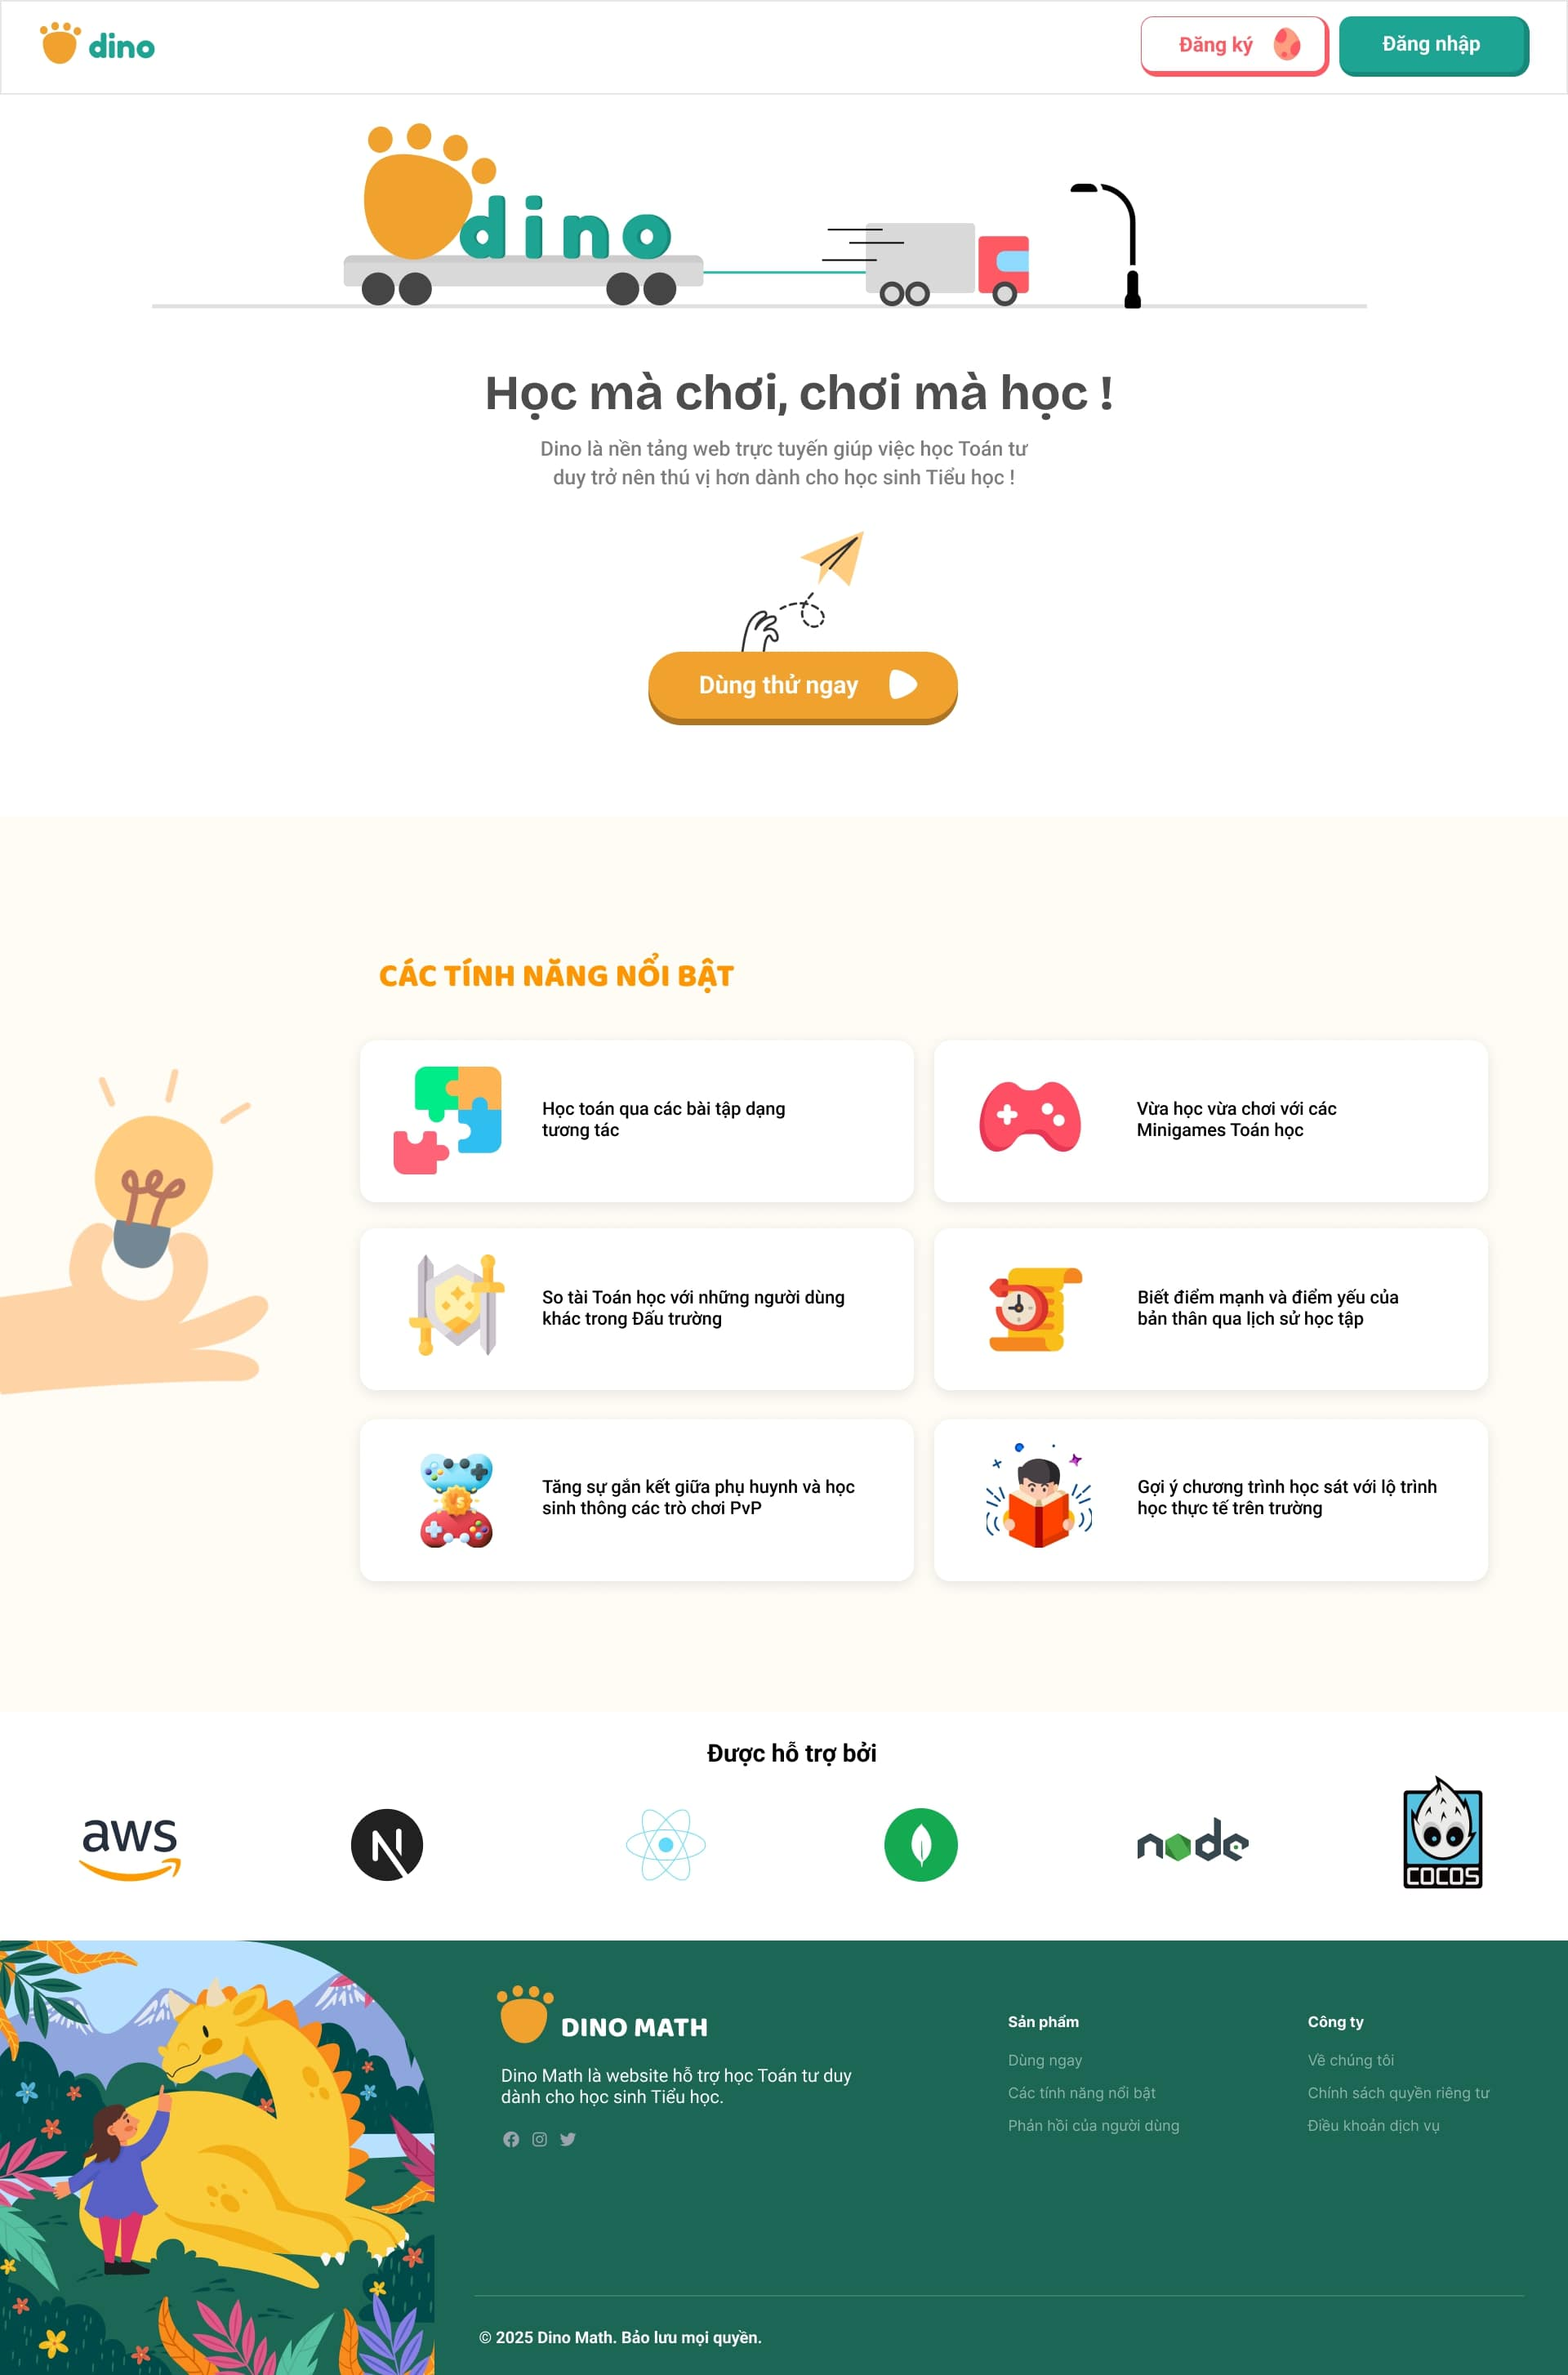
\includegraphics[width=0.9\textwidth]{Image/UI/LandingPage.jpg}
	\vspace{0.6cm}
	\caption{Landing Page}
	\label{fig:landingpage}
\end{figure}

\subsection{Giao diện đăng nhập và đăng ký tài khoản}
\subsubsection{Giao diện đăng nhập}
\label{subsubsec:login}
\begin{itemize}
	\item \textbf{Mục đích:} Cho phép người dùng xác thực tài khoản thông qua email và mật khẩu để truy cập và sử dụng các dịch vụ của hệ thống.
	\item \textbf{Mô tả:} 
	\begin{itemize}
		\item Giao diện đăng nhập ở giữa màn hình sẽ được hiển thị khi người dùng chọn tab \textit{Đăng nhập} ở thanh điều hướng bên trái.
		\item Có 2 phương thức để đăng nhập: Đăng nhập bằng tài khoản hệ thống hoặc Đăng nhập bằng tài khoản Google.
		\begin{itemize}
			\item Đối với chức năng Đăng nhập bằng tài khoản hệ thống, người dùng phải nhập thông tin đăng nhập vào các field \textit{Email} và \textit{Mật khẩu} như \textit{Hình \ref{fig:login}}. Nếu người dùng quên mật khẩu, có thể bấm vào link \textit{Quên mật khẩu} để truy cập vào trang \textbf{Lấy lại mật khẩu} được mô tả ở mục \ref{subsec:resetpassword}.
			Nút \textit{Đăng nhập} chỉ được enable khi giá trị của các field khác rỗng. Sau khi bấm đăng nhập, hệ thống sẽ tiến hành gửi request về backend để
			xác thực người dùng. Nếu thành công, người dùng sẽ được điều hướng về giao diện mặc định tùy theo loại tài khoản (đối với tài khoản học sinh, giao diện mặc định là \textbf{Trang chủ} được mô tả ở mục \ref{subsubsec:studenthome}, còn đối với phụ huynh là \textbf{Trang thống kê tổng quan} được mô tả ở mục \ref{subsubsec:parenthome}). Nếu thất bại, lỗi cụ thể sẽ được hiển thị dưới dạng toast message để thông báo cho người dùng như \textit{Hình \ref{fig:wrongpassword}}. Ngoài ra, đối với tài khoản học sinh, sau khi đăng nhập lần đầu tiên, người dùng sẽ được điều hướng đến giao diện \textbf{Onboarding} được mô tả ở mục \ref{subsec:onboarding} để cập nhật hồ sơ cá nhân.
			\begin{figure}[H]
				\centering
				
\includegraphics[width=0.9\textwidth]{Image/UI/Auth/Login.jpg}
				\vspace{0.6cm}
				\caption{Giao diện đăng nhập}
				\label{fig:login}
			\end{figure}
			\begin{figure}[H]
				\centering
				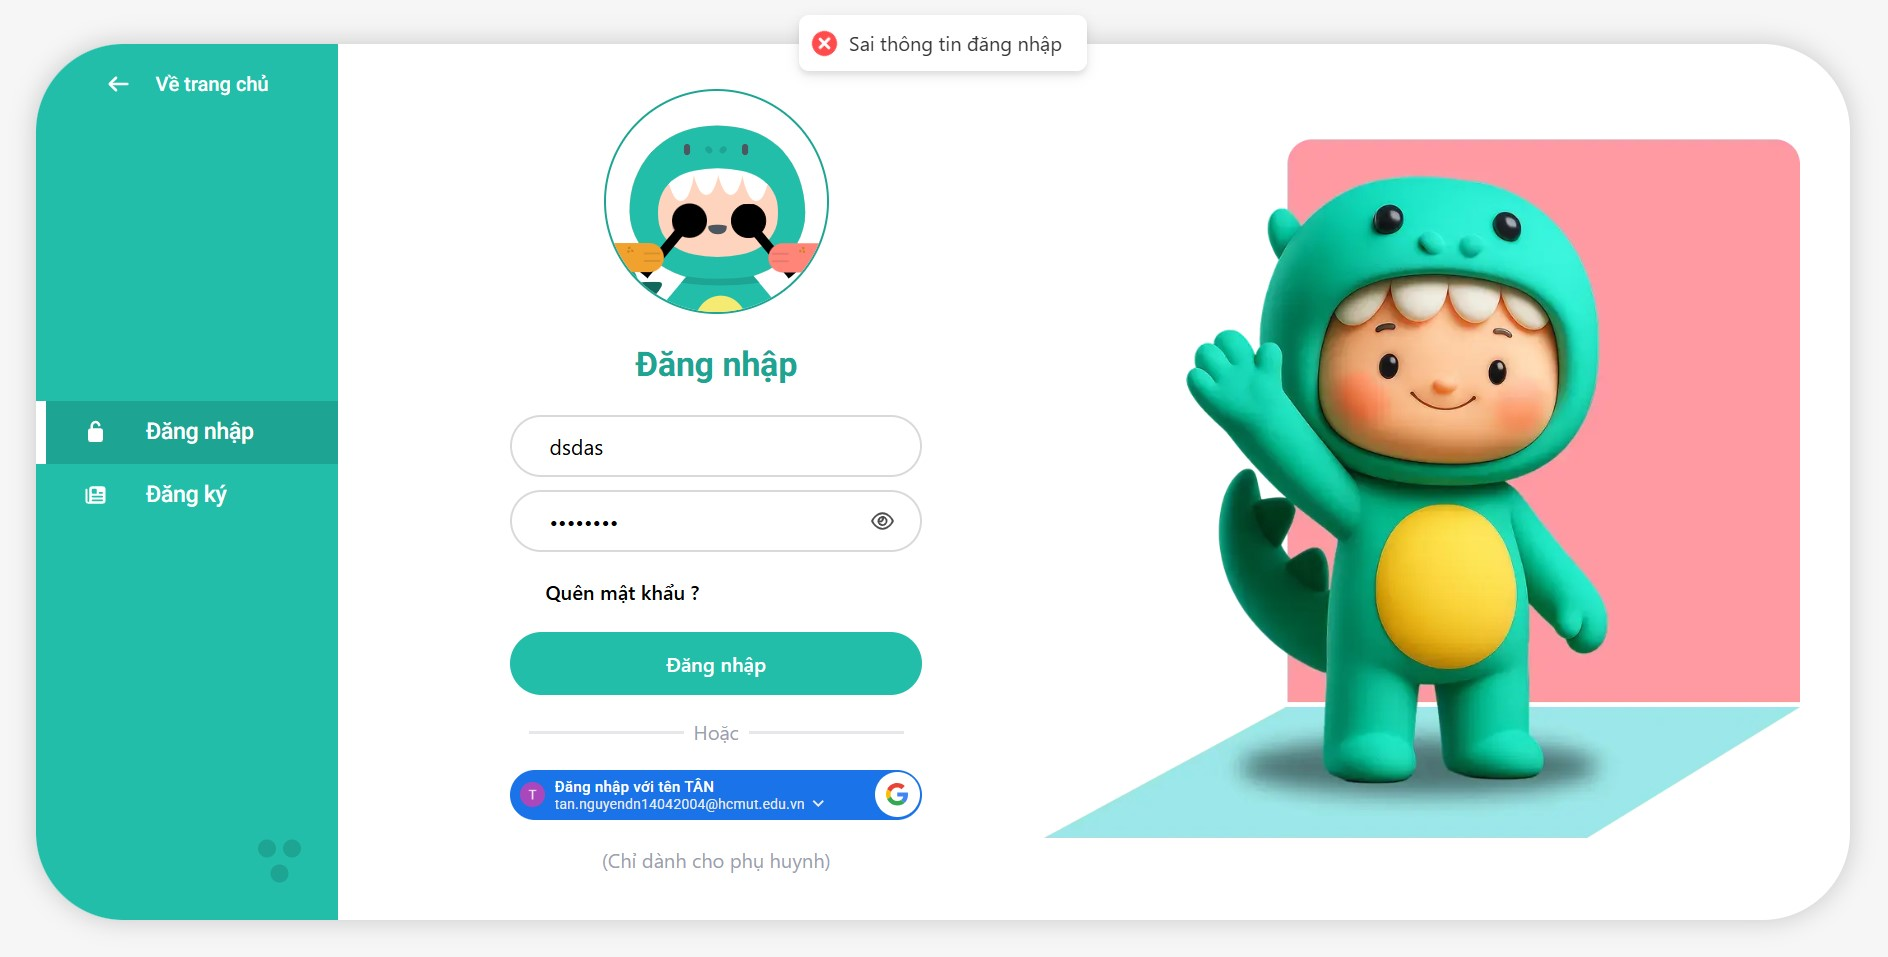
\includegraphics[width=0.9\textwidth]{Image/UI/Auth/LoginError.jpg}
				\vspace{0.6cm}
				\caption{Lỗi sai thông tin đăng nhập}
				\label{fig:wrongpassword}
			\end{figure}
			\item Đối với chức năng đăng nhập bằng Google (chỉ dành cho Phụ huynh), người dùng sẽ bấm vào nút \textit{Đăng nhập bằng Google}. Sau đó, người dùng thực hiện các thao tác đăng nhập bằng tài khoản Google trên cửa sổ mới. Nếu thành công, người dùng được điều hướng tới trang chủ của mình.
			\begin{figure}[H]
				\centering
				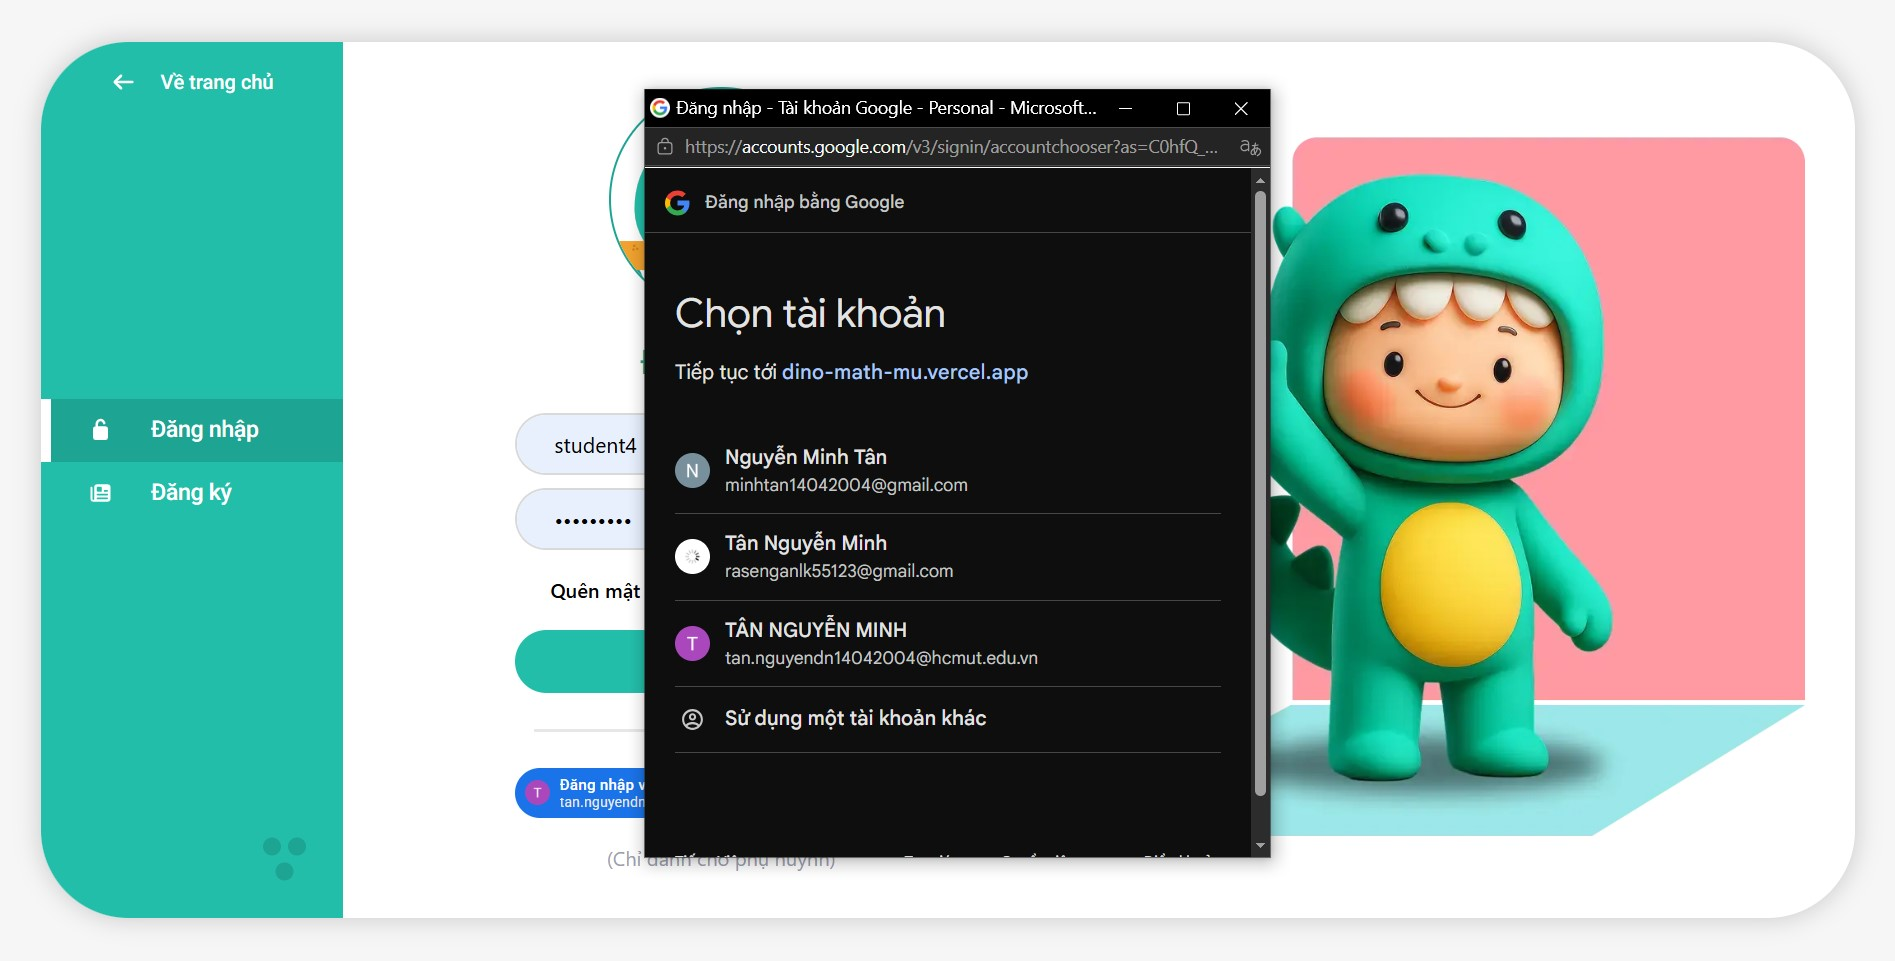
\includegraphics[width=0.9\textwidth]{Image/UI/Auth/OAuth.jpg}
				\vspace{0.6cm}
				\caption{Giao diện đăng nhập bằng Google}
				\label{fig:oauth}
			\end{figure}
		\end{itemize}
	\end{itemize}
\end{itemize}

\subsubsection{Giao diện đăng ký tài khoản}
\begin{itemize}
	\item \textbf{Mục đích:} Cho phép người dùng đăng ký tài khoản mới.
	\item \textbf{Mô tả:} Giao diện đăng ký sẽ được hiển thị khi người dùng chọn tab \textit{Đăng ký} ở thanh điều hướng bên trái. Giao diện đăng ký tài khoản bao gồm 2 bước:
	\begin{itemize}
		\item \textbf{Bước 1 - Chọn loại tài khoản}: Người dùng cần chọn 1 trong 2 loại tài khoản mà mình muốn tạo bao gồm: Phụ huynh hoặc Học sinh. Giao diện của bước này được mô tả như thiết kế như \textit{Hình \ref{fig:rolepick}} bên dưới. 
		\begin{figure}[H]
			\centering
			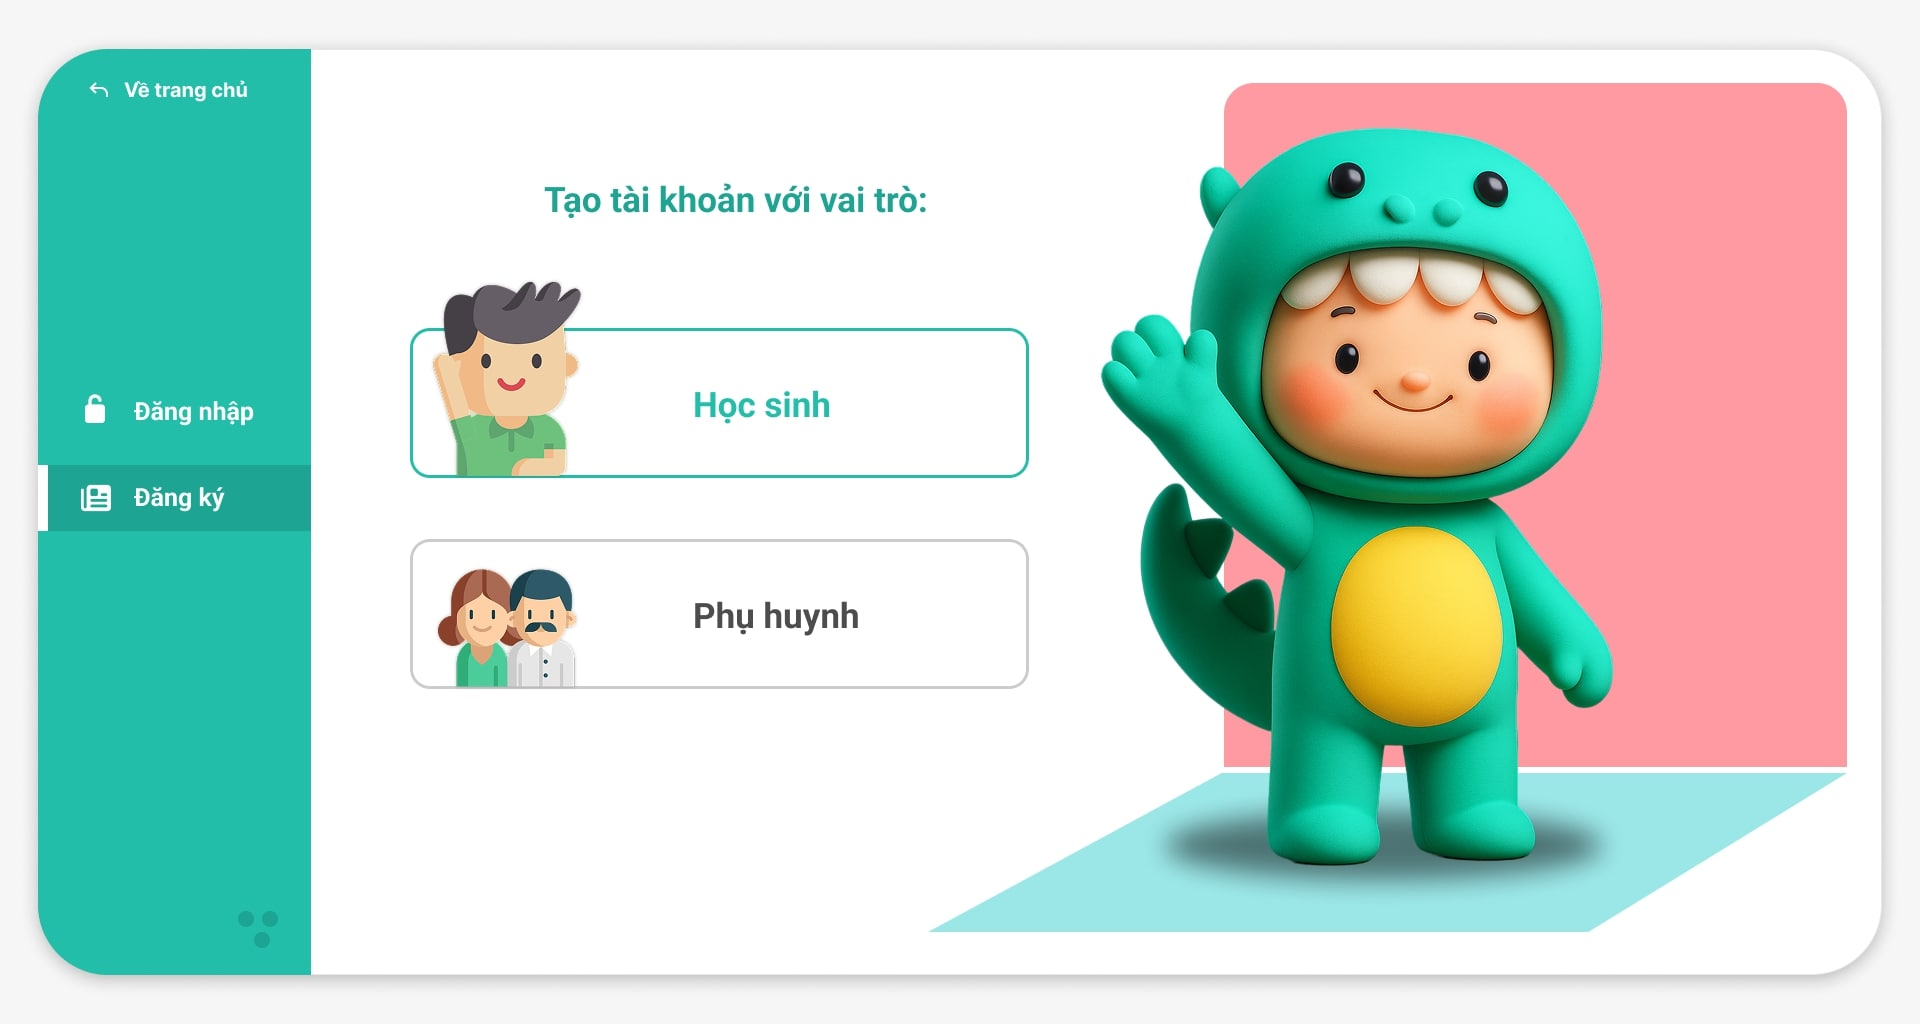
\includegraphics[width=0.9\textwidth]{Image/UI/Auth/SignUpPage-RolePicking.jpg}
			\vspace{0.6cm}
			\caption{Giao diện đăng ký tài khoản - Chọn loại tài khoản}
			\label{fig:rolepick}
		\end{figure}
		
		\item \textbf{Bước 2 - Nhập thông tin đăng ký}: Người dùng cần nhập  các thông tin bao gồm: Email (đối với phụ huynh) hoặc Tên tài khoản (đối với học sinh), Họ và tên, Mật khẩu và Xác nhận mật khẩu. Đối với thông tin về Họ và tên, thông tin này chỉ xuất hiện khi người dùng chọn đăng ký tài khoản Phụ huynh, còn đối với Học sinh, thông tin này sẽ được bổ sung sau ở giao diện \textbf{Onboarding} được mô tả ở mục \ref{subsec:onboarding}.
		Nút \textit{Đăng ký} chỉ được enable khi các điều kiện sau được thỏa mãn:
		\begin{itemize}
			\item Giá trị của tất cả các field khác rỗng.
			\item Mật khẩu có ít nhất 8 ký tự, trong đó phải chứa chữ cái in hoa, chữ thường, số và ký tự đặc biệt.
			\item Mật khẩu và Xác nhận mật khẩu phải trùng khớp.
		\end{itemize}
		Giao diện của bước 2 được thiết kế như \textit{Hình \ref{fig:regstudent}} và \textit{Hình \ref{fig:regparent}} bên dưới.
		\begin{figure}[H]
			\centering
			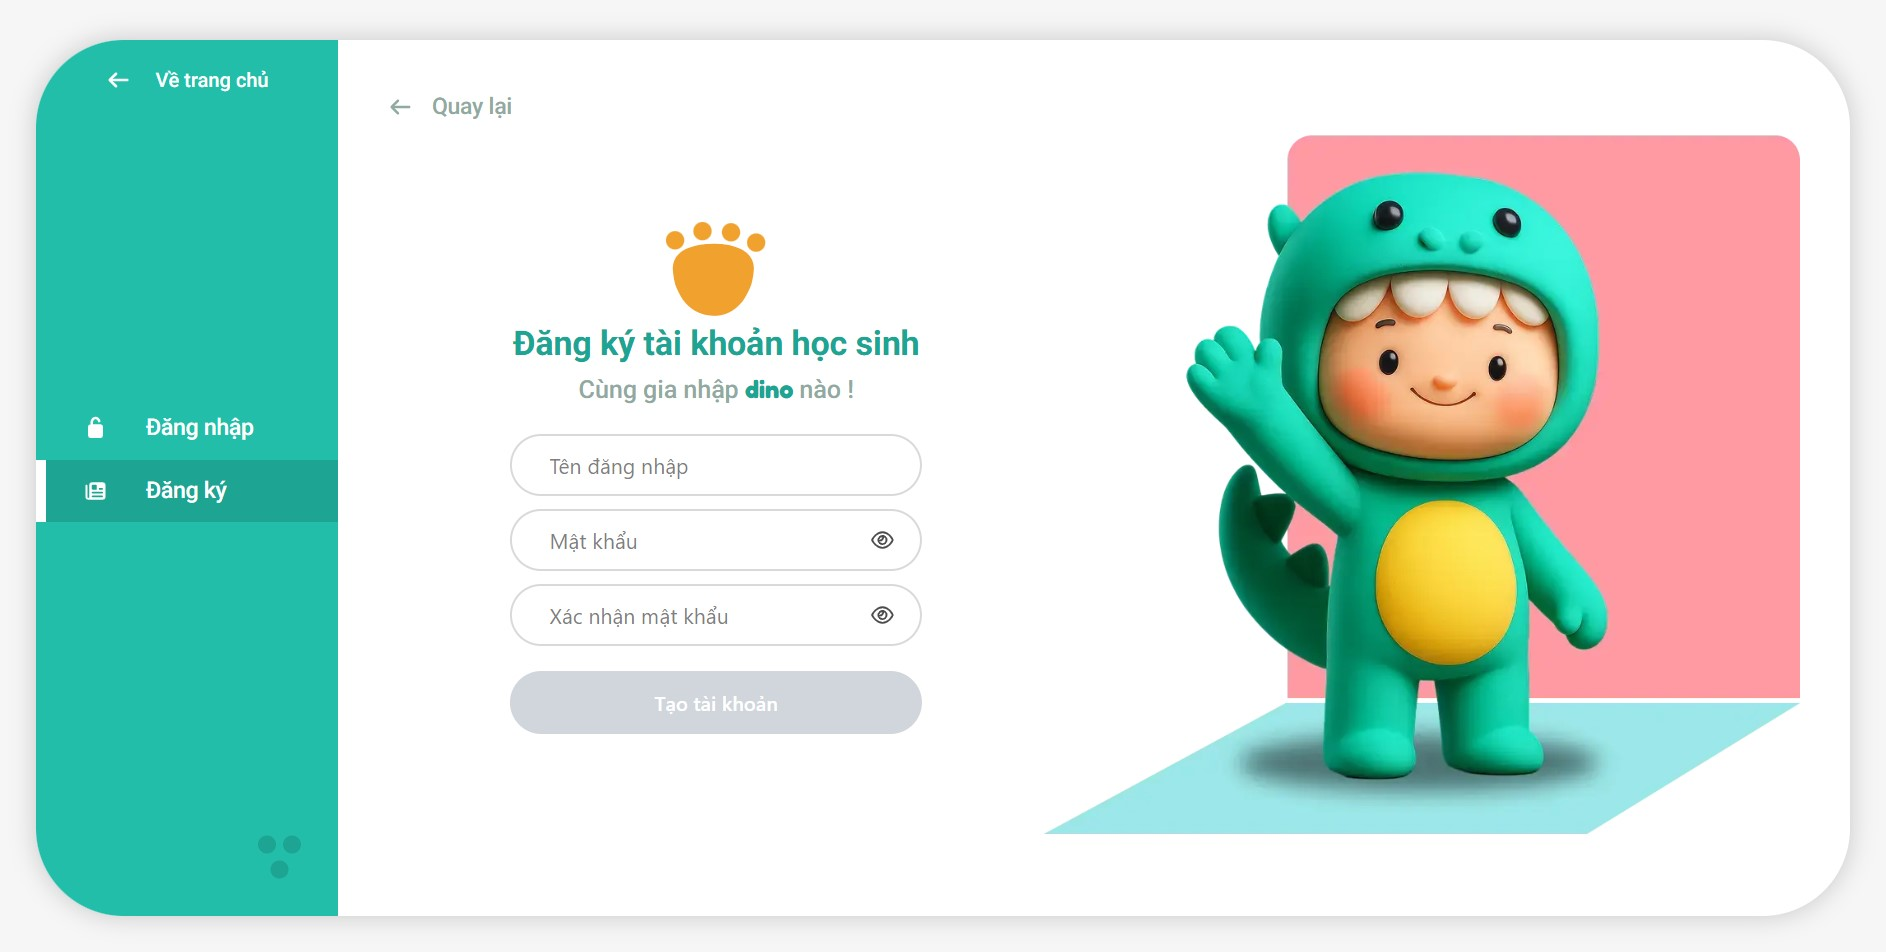
\includegraphics[width=0.9\textwidth]{Image/UI/Auth/StudentRegister.jpg}
			\vspace{0.6cm}
			\caption{Giao diện đăng ký tài khoản - Học sinh}
			\label{fig:regstudent}
		\end{figure}
		\begin{figure}[H]
			\centering
			
\includegraphics[width=0.9\textwidth]{Image/UI/Auth/ParentRegister.jpg}
			\vspace{0.6cm}
			\caption{Giao diện đăng ký tài khoản - Phụ huynh}
			\label{fig:regparent}
		\end{figure}
		
		\item \textbf{Bước 3 - Bấm đăng ký tài khoản}: Sau khi tất cả thông tin hợp lệ, người dùng có thể bấm nút đăng ký tài khoản để tiến hành tạo tài khoản mới. Thông báo đăng ký thành công hoặc thất bại sẽ được hiển thị dưới dạng toast message được thiết kế như \textit{Hình \ref{fig:regerror}} và \textit{Hình \ref{fig:success}} bên dưới.
	\end{itemize}
	\begin{figure}[H]
		\centering
		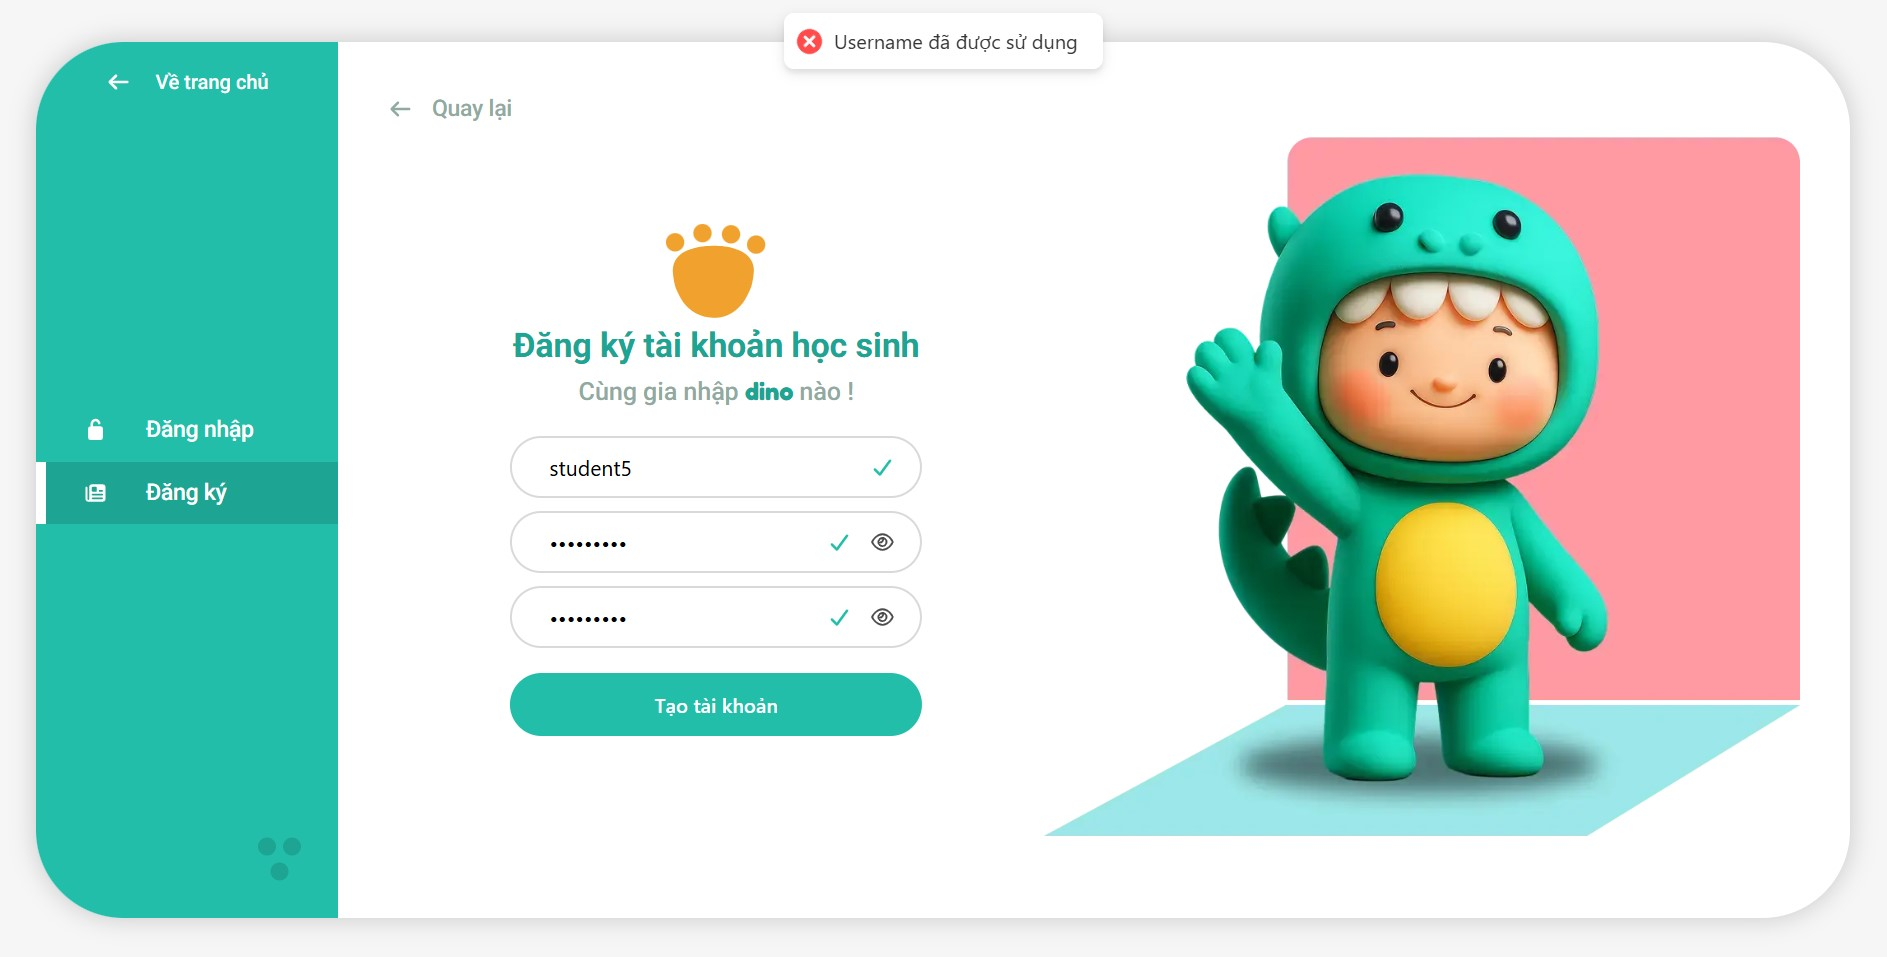
\includegraphics[width=0.9\textwidth]{Image/UI/Auth/UserExist.jpg}
		\vspace{0.6cm}
		\caption{Giao diện đăng ký tài khoản - Lỗi username đã được sử dụng}
		\label{fig:regerror}
	\end{figure}
	\begin{figure}[H]
		\centering
		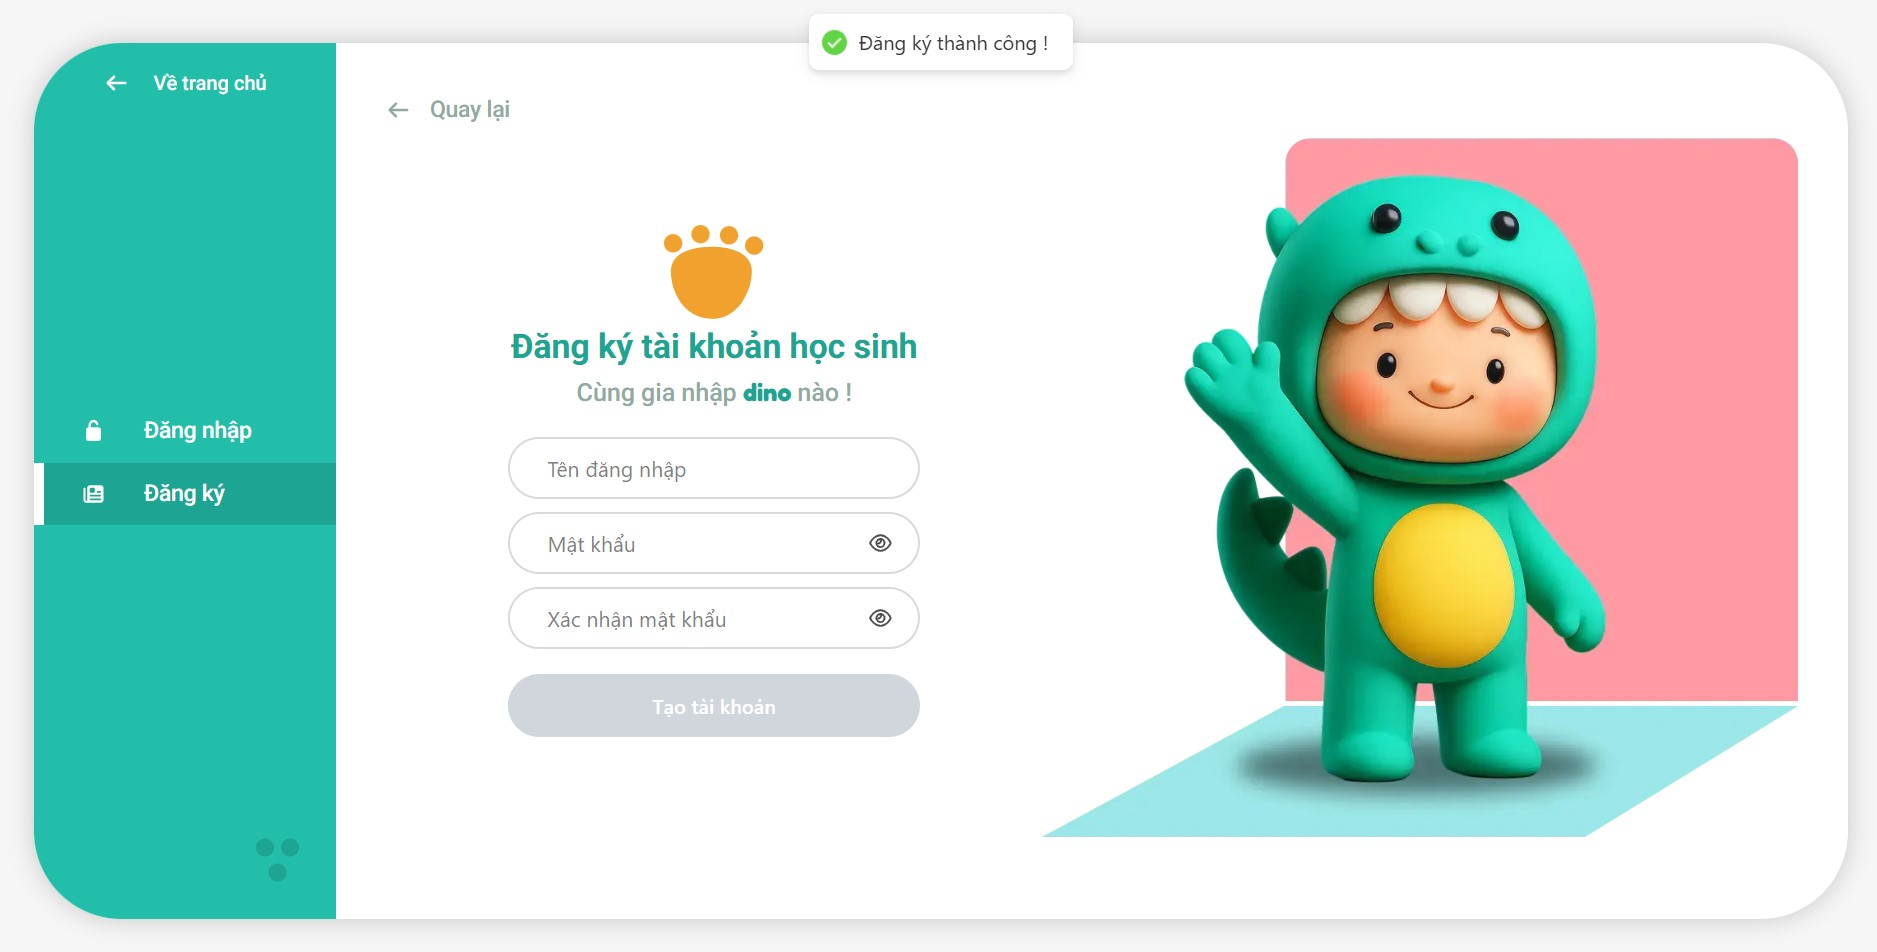
\includegraphics[width=0.9\textwidth]{Image/UI/Auth/RegisterSuccess.jpg}
		\vspace{0.6cm}
		\caption{Giao diện đăng ký tài khoản thành công}
		\label{fig:success}
	\end{figure}
\end{itemize}}

\subsection{Giao diện Onboarding}
\label{subsec:onboarding}
\begin{itemize}
	\item \textbf{Mục đích:} 
	\begin{itemize}
		\item Cho phép người dùng là Học sinh cập nhật thông tin của mình khi đăng nhập lần đầu tiên. 
		\item Cung cấp giao diện tương tác với Linh vật động của hệ thống, tạo cảm giác hứng thú và gần gũi đối với đối tượng người dùng chính là học sinh Tiểu học.
	\end{itemize}
	\item \textbf{Mô tả:} 
	Giao diện Onboarding bao gồm 3 bước như sau:
	\begin{itemize}
		\item \textbf{Bước 1 - Nhập thông tin cá nhân bao gồm họ tên và khối lớp (1-5)}: Học sinh cần nhập Họ và tên cũng như chọn Khối lớp mà mình đang học ở ô dropdown. Nút Tiếp tục chỉ được enable khi tất cả các thông tin đã được điền. Giao diện của bước 1 được thiết kế như \textit{Hình \ref{fig:onboarding}} bên dưới.
		\begin{figure}[H]
			\centering
			
\includegraphics[width=0.9\textwidth]{Image/UI/Auth/Onboarding-Info.jpg}
			\vspace{0.6cm}
			\caption{Giao diện Onboarding - Nhập Họ tên và Khối lớp}
			\label{fig:onboarding}
		\end{figure}
		
		\item \textbf{Bước 2 - Cập nhật ảnh đại diện}: Học sinh có thể chọn ảnh đại diện có sẵn của hệ thống hoặc ảnh tự chọn. Giao diện của bước 2 được thiết kế như \textit{Hình \ref{fig:avatar}} bên dưới.
		\begin{figure}[H]
			\centering
			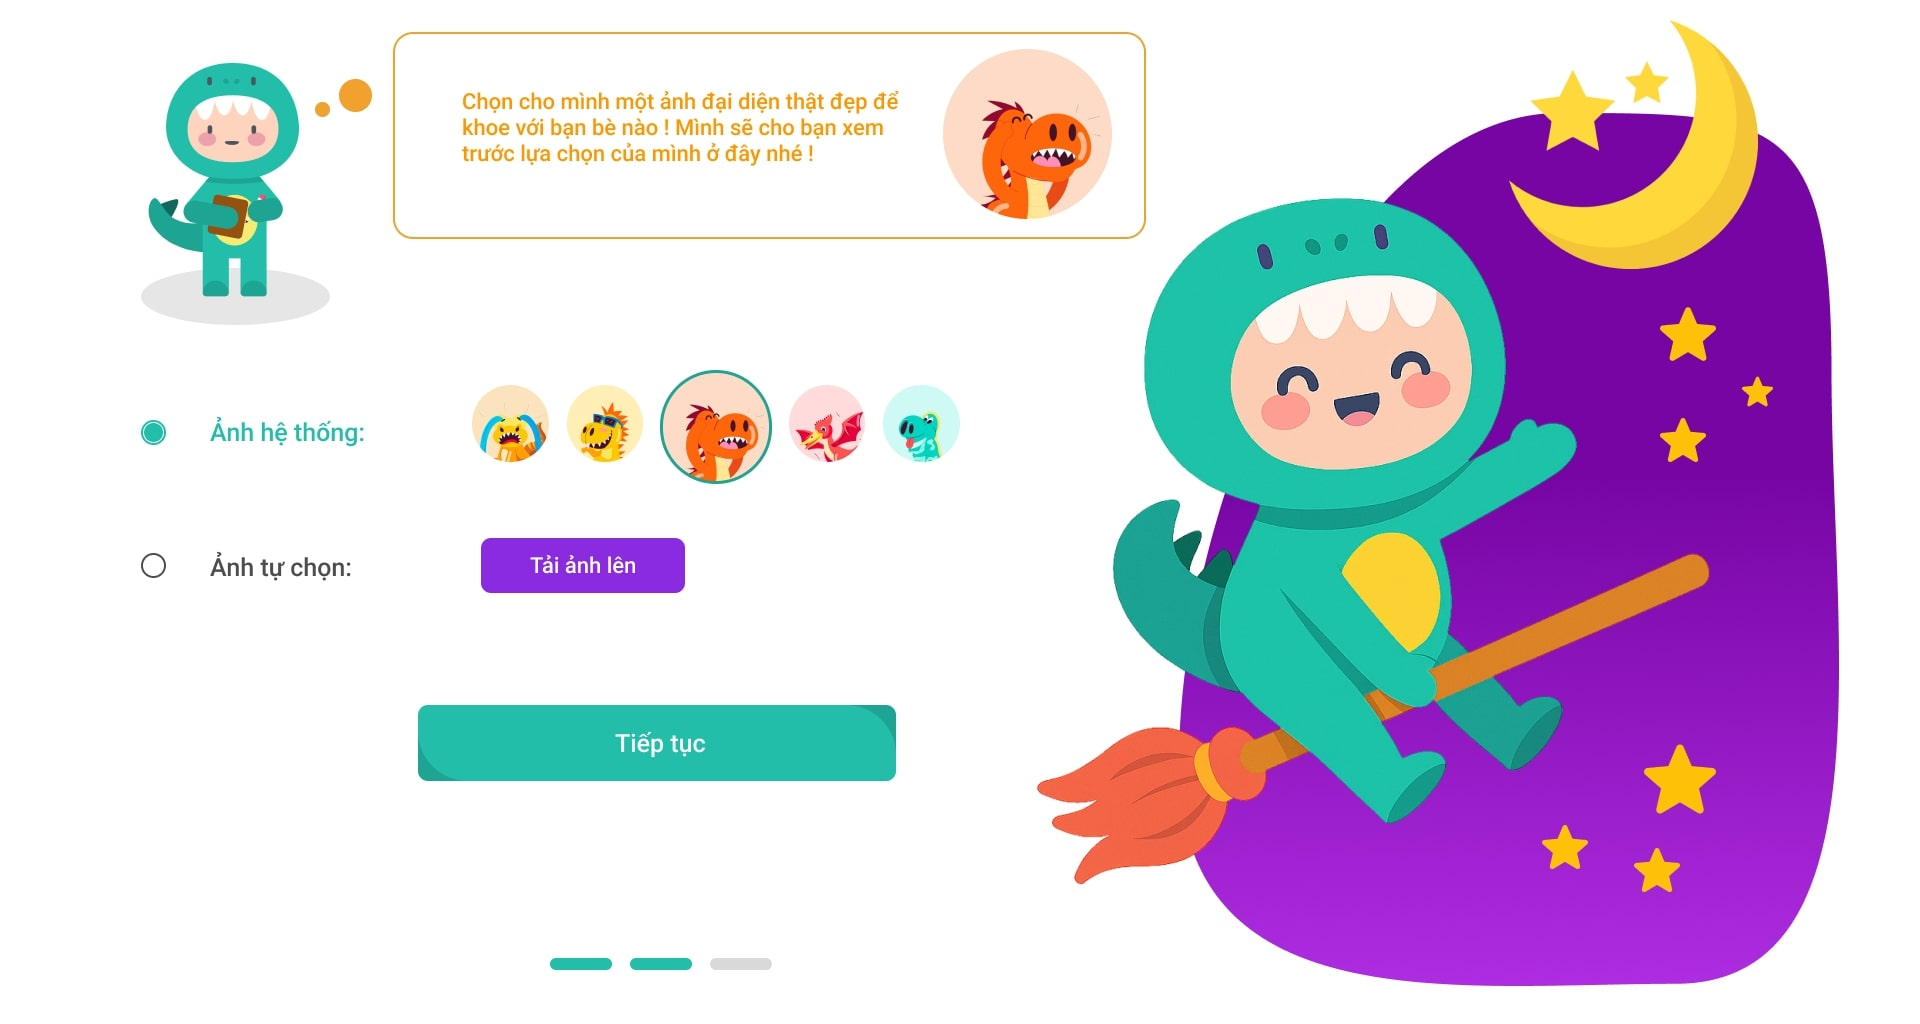
\includegraphics[width=0.9\textwidth]{Image/UI/Auth/Onboarding-Avatar.jpg}
			\vspace{0.6cm}
			\caption{Giao diện Onboarding - Cập nhật ảnh đại diện}
			\label{fig:avatar}
		\end{figure}
		
		\item \textbf{Bước 3 - Nhập mã liên kết tài khoản}: Hệ thống sẽ được tổ chức thành các Family (Gia đình), mỗi gia đình được quản lý bởi một tài khoản Phụ huynh duy nhất. Mã liên kết hay mã mời là mã mà Phụ huynh gửi cho Học sinh để liên kết vào Family của Phụ huynh đó. Ở bước Nhập mã liên kết, Học sinh có thể để trống field này và có thể thực hiện liên kết sau khi đã đăng nhập. Giao diện của bước 3 được thiết kế như \textit{Hình \ref{fig:link}} bên dưới.
		\begin{figure}[H]
			\centering
			
\includegraphics[width=0.9\textwidth]{Image/UI/Auth/Onboarding-InviteCode.jpg}
			\vspace{0.6cm}
			\caption{Giao diện Onboarding - Nhập mã liên kết tài khoản}
			\label{fig:link}
		\end{figure}
		\item Sau khi bấm hoàn thành, học sinh sẽ được điều hướng về \textbf{Trang chủ} của mình được mô tả ở mục \ref{subsubsec:studenthome}.
	\end{itemize}
\end{itemize}

\newpage
\subsection{Giao diện Lấy lại mật khẩu}
\label{subsec:resetpassword}
\begin{itemize}
	\item \textbf{Mục đích:} Giúp người dùng lấy lại mật khẩu thông qua xác thực OTP được gửi đến email.
	\item \textbf{Mô tả:} 
	Khi người dùng bấm vào link \textit{Quên mật khẩu} ở giao diện đăng nhập, trang lấy lại mật khẩu sẽ được hiển thị. Giao diện Lấy lại mật khẩu bao gồm 3 bước như sau:
	\begin{itemize}
		\item \textbf{Bước 1 - Gửi OTP qua email}: Người dùng cần nhập địa chỉ Email (nếu là phụ huynh) và Tên tài khoản (nếu là học sinh) vào ô trống và bấm nút \textit{Gửi mã xác thực}. Sau đó, một email kèm OTP sẽ được gửi đến địa chỉ email của phụ huynh. Nếu người dùng là học sinh, cần liên hệ với phụ huynh để nhận OTP. Giao diện của bước 1 được thiết kế như \textit{Hình \ref{fig:sendotp}} bên dưới.
		\begin{figure}[H]
			\centering
			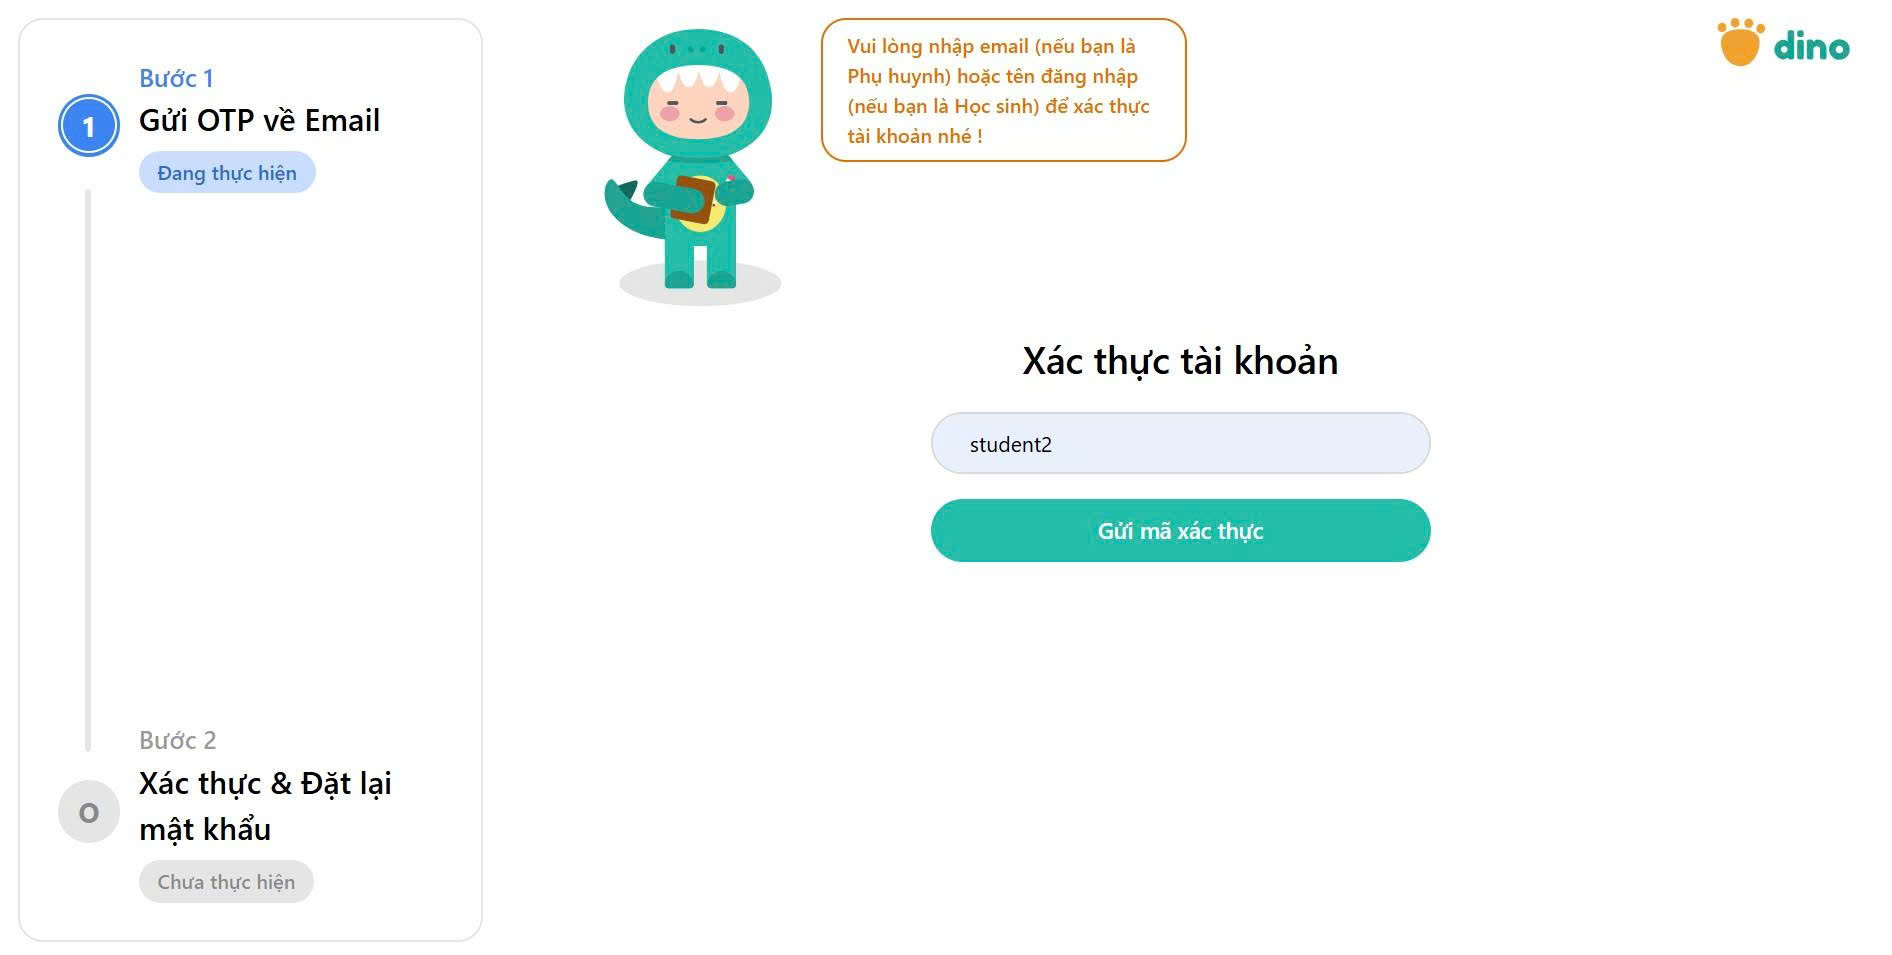
\includegraphics[width=0.9\textwidth]{Image/UI/Auth/PasswordReset1.jpg}
			\vspace{0.6cm}
			\caption{Giao diện Lấy lại mật khẩu - Bước 1}
			\label{fig:sendotp}
		\end{figure}
		
		\item \textbf{Bước 2 - Xác thực OTP và đổi mật khẩu}: Người dùng cần nhập mã OTP được cung cấp, sau đó điền mật khẩu mới của mình vào các textbox tương ứng.  Nút \textit{Đổi mật khẩu} chỉ được enable khi:
		\begin{itemize}
			\item Giá trị của tất cả các field khác rỗng.
			\item Mật khẩu có ít nhất 8 ký tự, trong đó phải chứa chữ cái in hoa, chữ thường, số và ký tự đặc biệt.
			\item Mật khẩu và Xác nhận mật khẩu phải trùng khớp.
		\end{itemize}
		Giao diện của bước 2 được thiết kế như \textit{Hình \ref{fig:inputotp}} bên dưới.
		\begin{figure}[H]
			\centering
			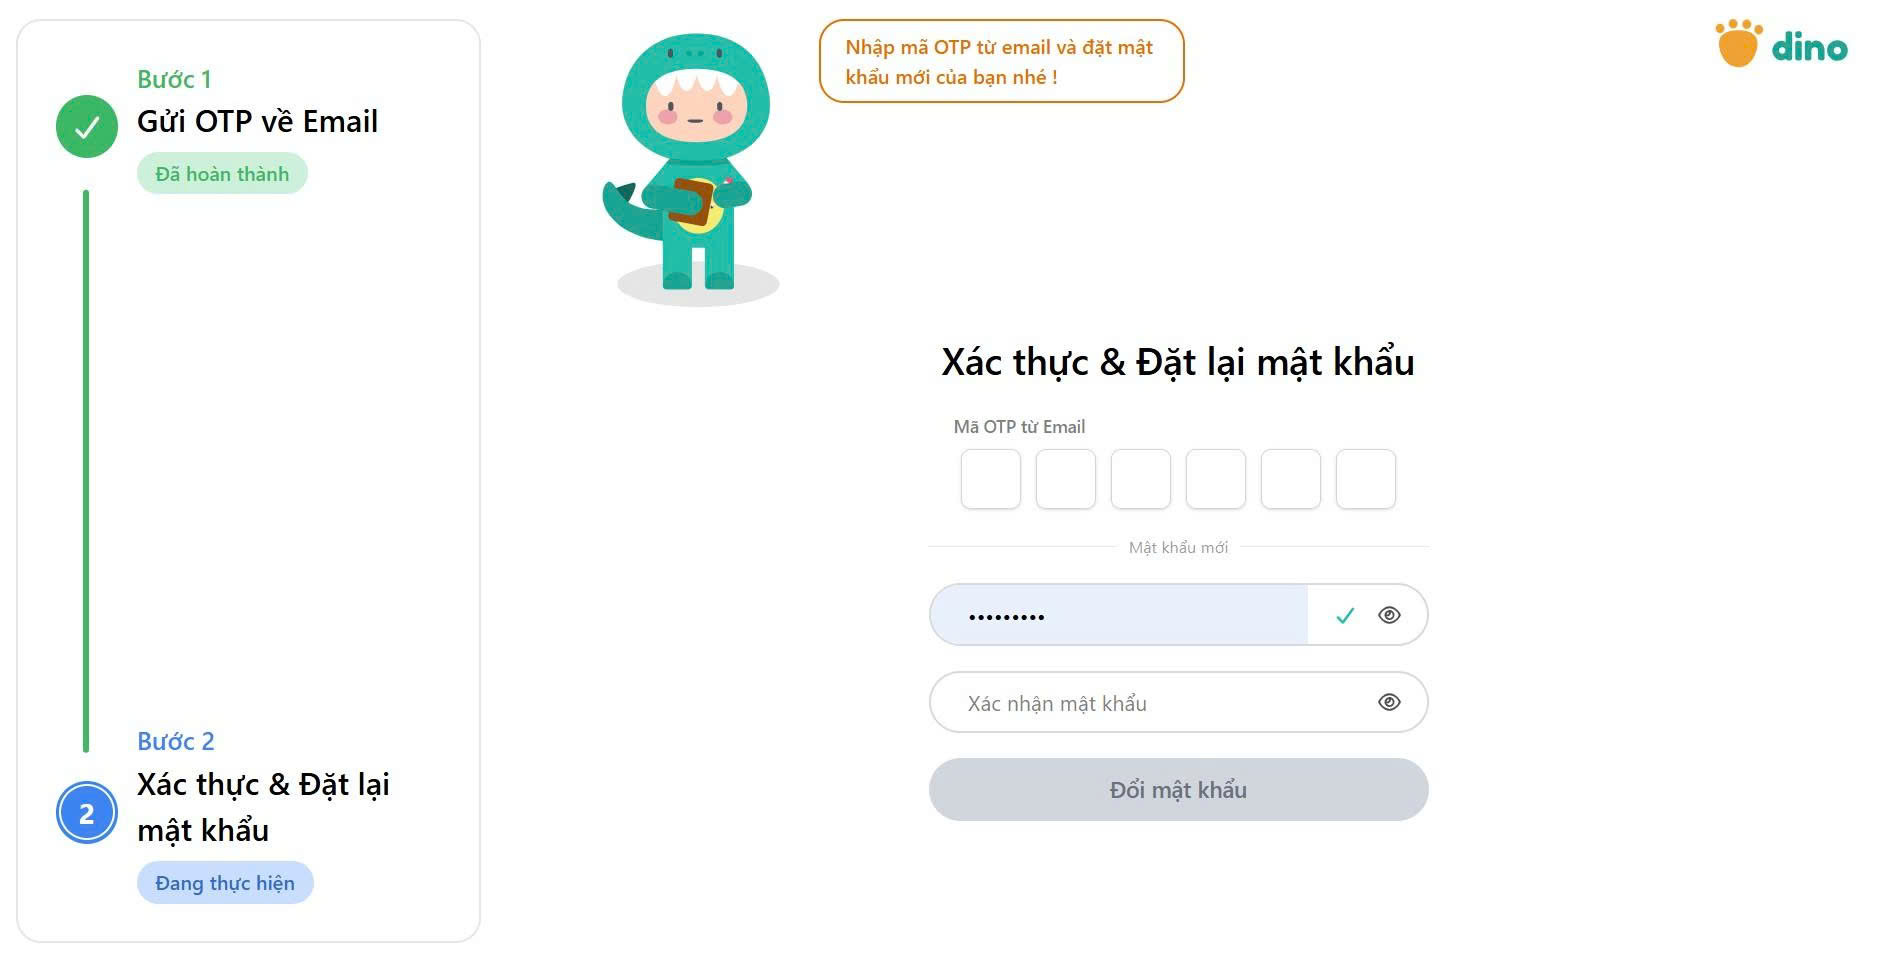
\includegraphics[width=0.9\textwidth]{Image/UI/Auth/PasswordReset2.jpg}
			\vspace{0.6cm}
			\caption{Giao diện Lấy lại mật khẩu - Bước 2}
			\label{fig:inputotp}
		\end{figure}
		
		\item Sau khi đổi mật khẩu thành công, người dùng sẽ nhận được thông báo và được điều hướng về \textbf{Trang đăng nhập} được mô tả ở mục \ref{subsubsec:login}.
	\end{itemize}
\end{{itemize}

\subsection{Các màn hình chính của tài khoản Học sinh}
\textbf{Mô tả tổng quan}
Layout chính của giao diện bao gồm 2 phần: 
\begin{itemize}
	\item \textbf{Thanh điều hướng:} Nằm trên cùng chứa logo thương hiệu của website, các nút điều hướng, nút mở hồ sơ cá nhân, nút thông báo vào nút đăng xuất. Các nút điều hướng tương ứng với từng trang tính năng của website, bao gồm:
	\begin{itemize}
		\item Trang chủ (Nhà)
		\item Trang Bài học
		\item Trang Đấu trường
		\item Trang Bảng xếp hạng
		\item Trang Nhiệm vụ
		\item Trang Minigames
		\item Trang Lịch sử làm bài
	\end{itemize}
	\item \textbf{Phần nội dung} Chiếm phần còn lại của layout, là nơi thể hiện nội dung của các trang tính năng.
\end{itemize}
Layout tổng thể của các màn hình chức năng chính được minh họa thông qua giao diện trang chủ được thiết kế như hình bên dưới.
\begin{figure}[H]
	\centering
	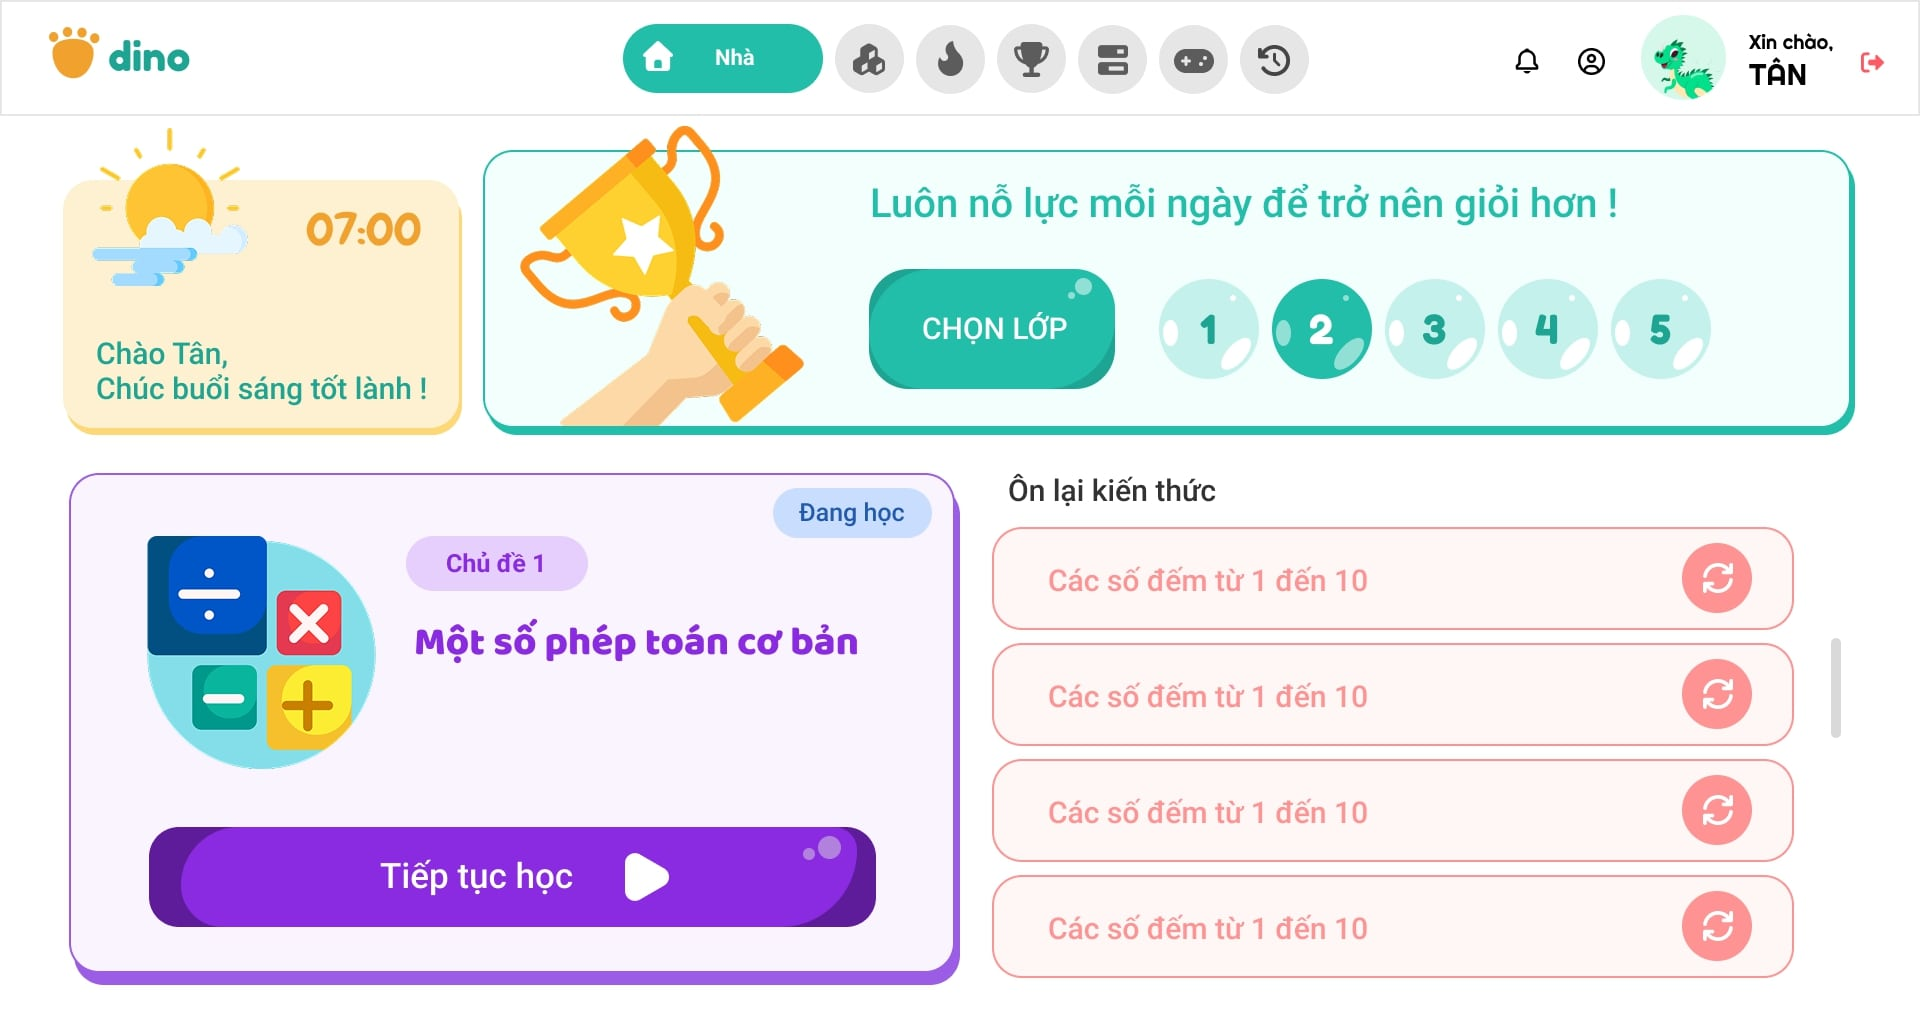
\includegraphics[width=0.9\textwidth]{Image/UI/Main-Student/Home-Morning.jpg}
	\vspace{0.6cm}
	\caption{Trang chủ (minh họa cho layout tổng thể)}
\end{figure}

\subsubsection{Trang chủ}
\label{subsubsec:studenthome}
Trang chủ là trang hiển thị mặc định ngay sau khi học sinh đăng nhập thành công vào hệ thống. Trang chủ có hiển thị giờ giấc và lời chào dành cho người dùng nhằm tạo cảm giác thân thiện và gần gũi. Các thẻ hiển thị giờ và lời chào sẽ thay đổi kiểu thiết kế tùy thuộc vào thời gian trong ngày (Sáng, Chiều, Tối). Giao diện trang chủ vào buổi sáng, buổi chiều và buổi tối được thiết kế lần lượt như các hình \ref{fig:homemorning}, \ref{fig:homeafternoon} và \ref{fig:homenight}. 
\begin{figure}[H]
	\centering
	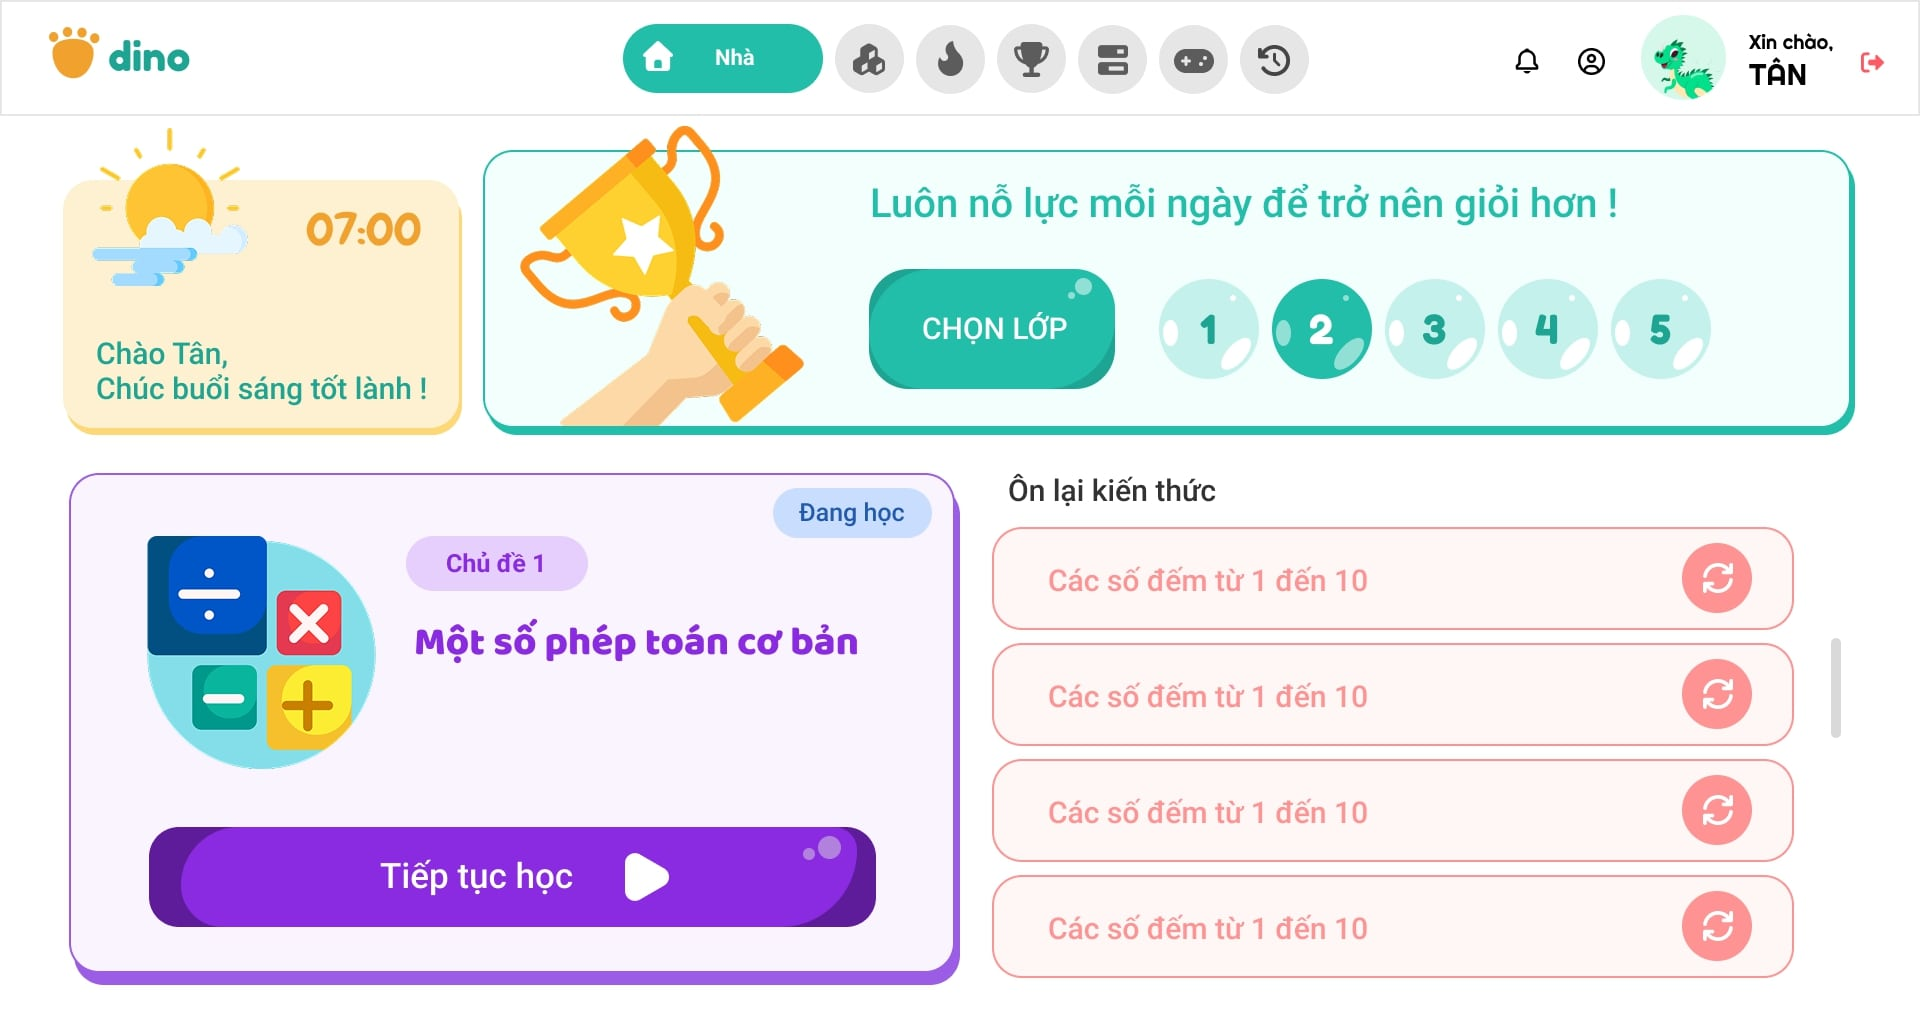
\includegraphics[width=0.9\textwidth]{Image/UI/Main-Student/Home-Morning.jpg}
	\vspace{0.6cm}
	\caption{Trang chủ - Buổi sáng}
	\label{fig:homemorning}
\end{figure}
\begin{figure}[H]
	\centering
	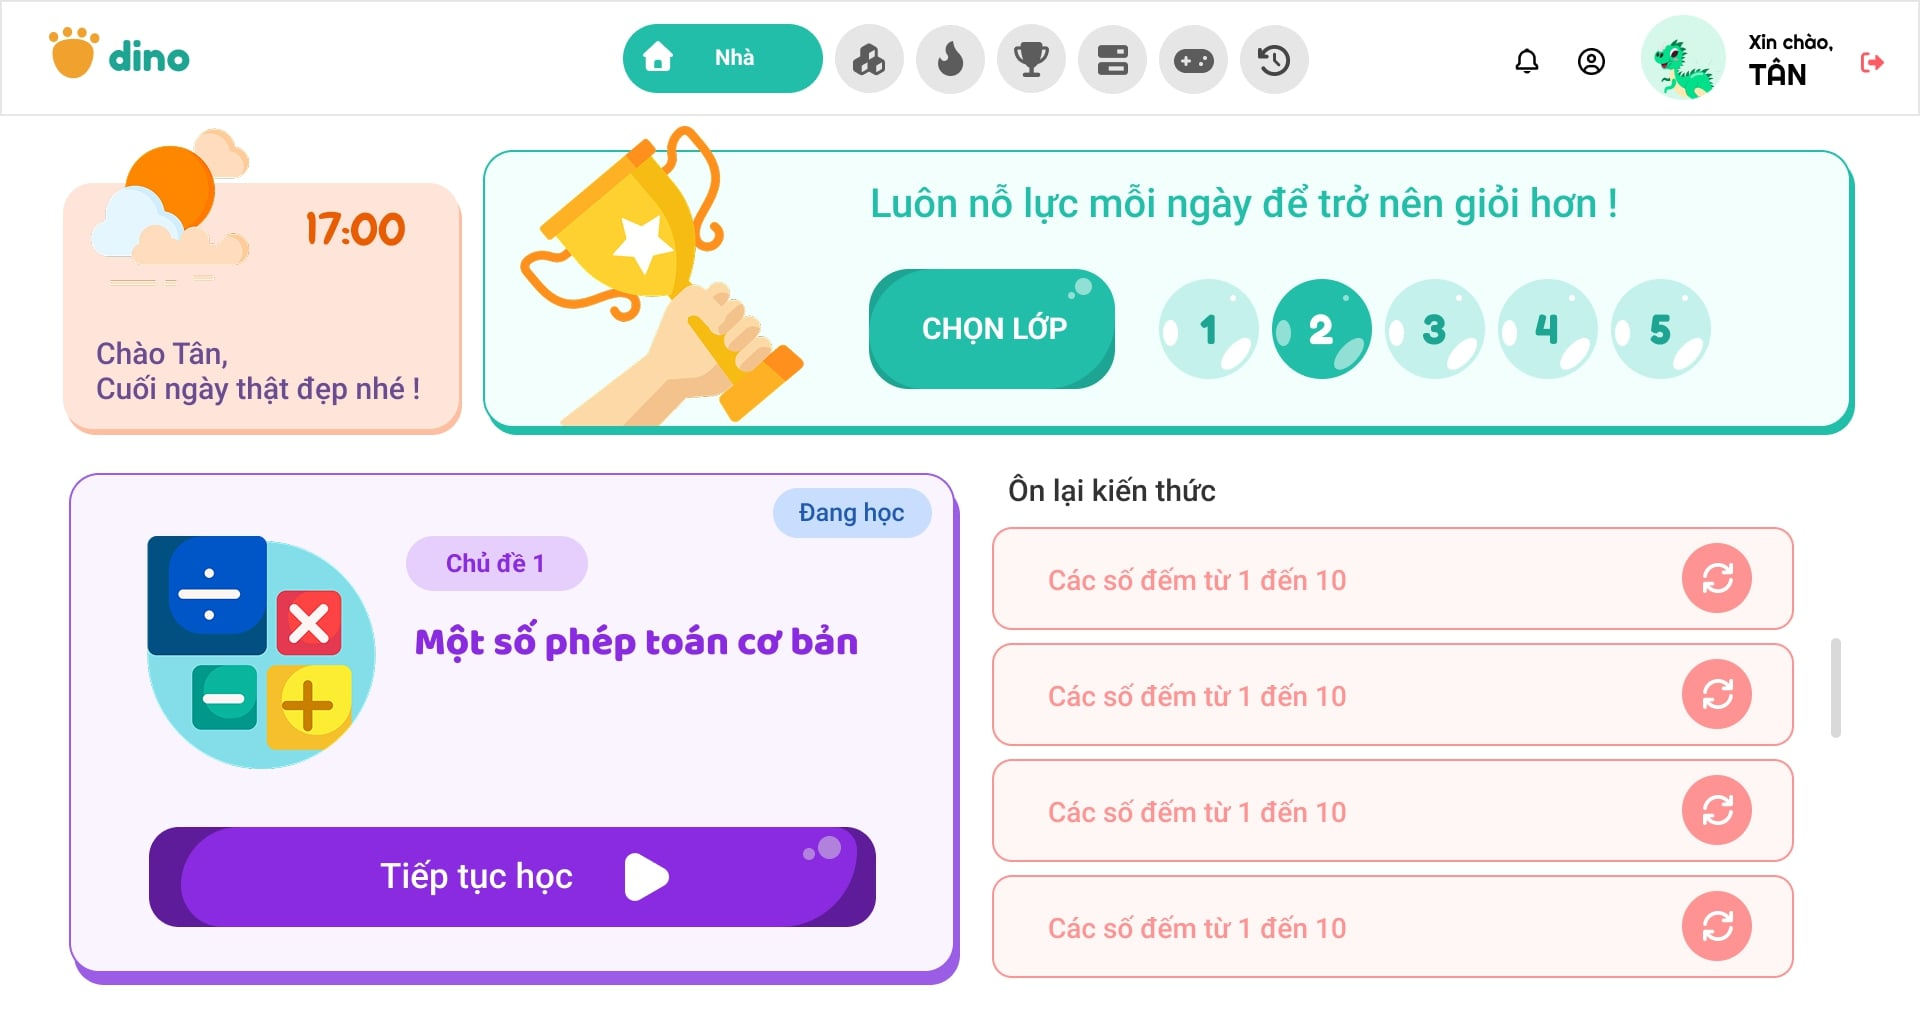
\includegraphics[width=0.9\textwidth]{Image/UI/Main-Student/Home-Afternoon.jpg}
	\vspace{0.6cm}
	\caption{Trang chủ - Buổi chiều}
	\label{fig:homeafternoon}
\end{figure}
\begin{figure}[H]
	\centering
	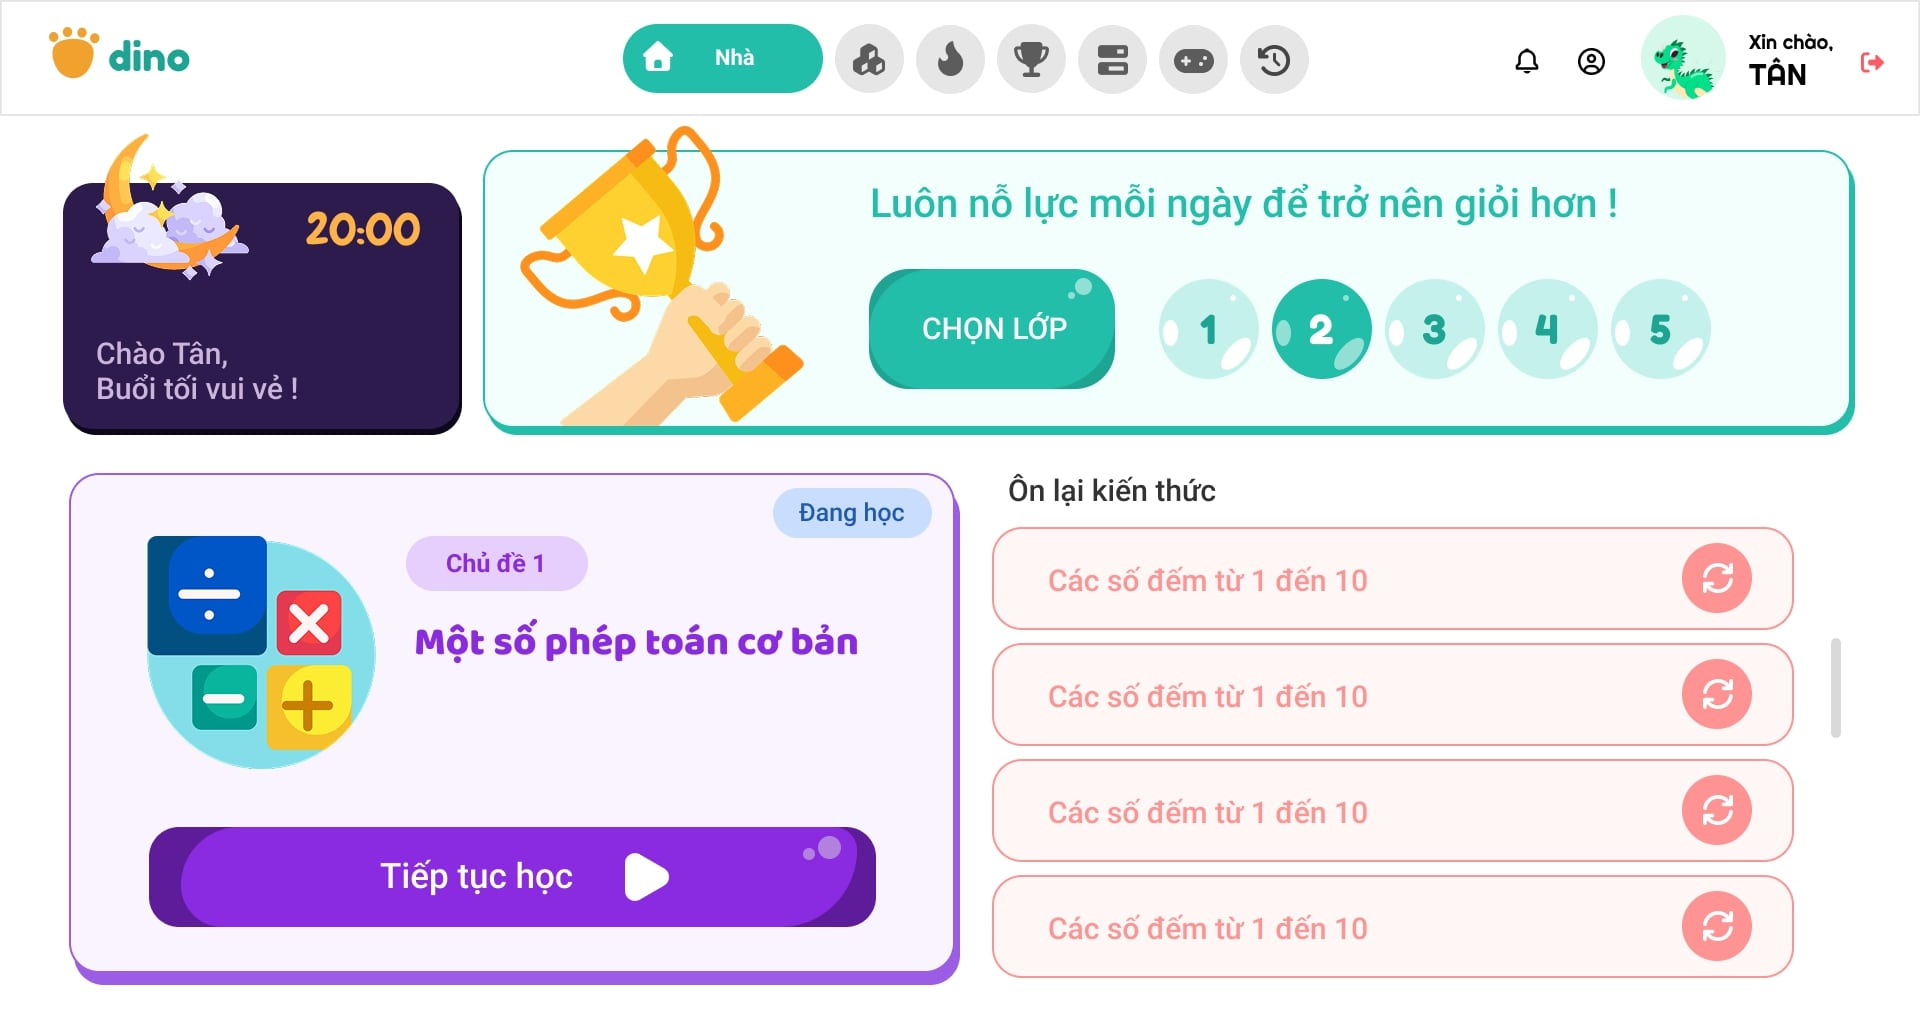
\includegraphics[width=0.9\textwidth]{Image/UI/Main-Student/Home-Night.jpg}
	\vspace{0.6cm}
	\caption{Trang chủ - Buổi tối}
	\label{fig:homenight}
\end{figure}

\vspace{0.2cm}
\newline
Học sinh có thể chọn lớp mình muốn học bằng cách nhấp chuột vào các bong bóng được đánh số từ 1-5. Việc thay đổi lớp ở Trang chủ sẽ không làm thay đổi thông tin về khối lớp trong hồ sơ người dùng.

\vspace{0.2cm}
\newline
Tại trang chủ, hệ thống hiển thị chủ đề gần nhất mà người dùng đã truy cập. Người dùng có thể nhanh chóng quay lại bài học bằng cách nhấn nút \textit{Tiếp tục học}. Bên cạnh đó, các chủ đề đã hoàn thành cũng được liệt kê trong mục \textit{Ôn lại kiến thức} đi kèm với biểu tượng 'Review'. Cả hai thao tác này đều điều hướng người dùng đến cùng một giao diện chi tiết của chủ đề (được mô tả cụ thể tại mục \ref{subsubsec:topic}).

\vspace{0.2cm}
\newpage
Khi người dùng truy cập vào Trang chủ, một thông báo sẽ được hiển thị dưới dạng popup được thiết kế như \textit{Hình \ref{fig:recommend}}. Popup này chứa thông tin gợi ý chủ đề học theo thời gian và khối lớp của người dùng. Người dùng có thể bấm nút \textit{Học ngay} để điều hướng đến trang chủ đề tương ứng được mô tả ở mục \ref{subsubsec:topic}. 
	\begin{figure}[H]
		\centering
		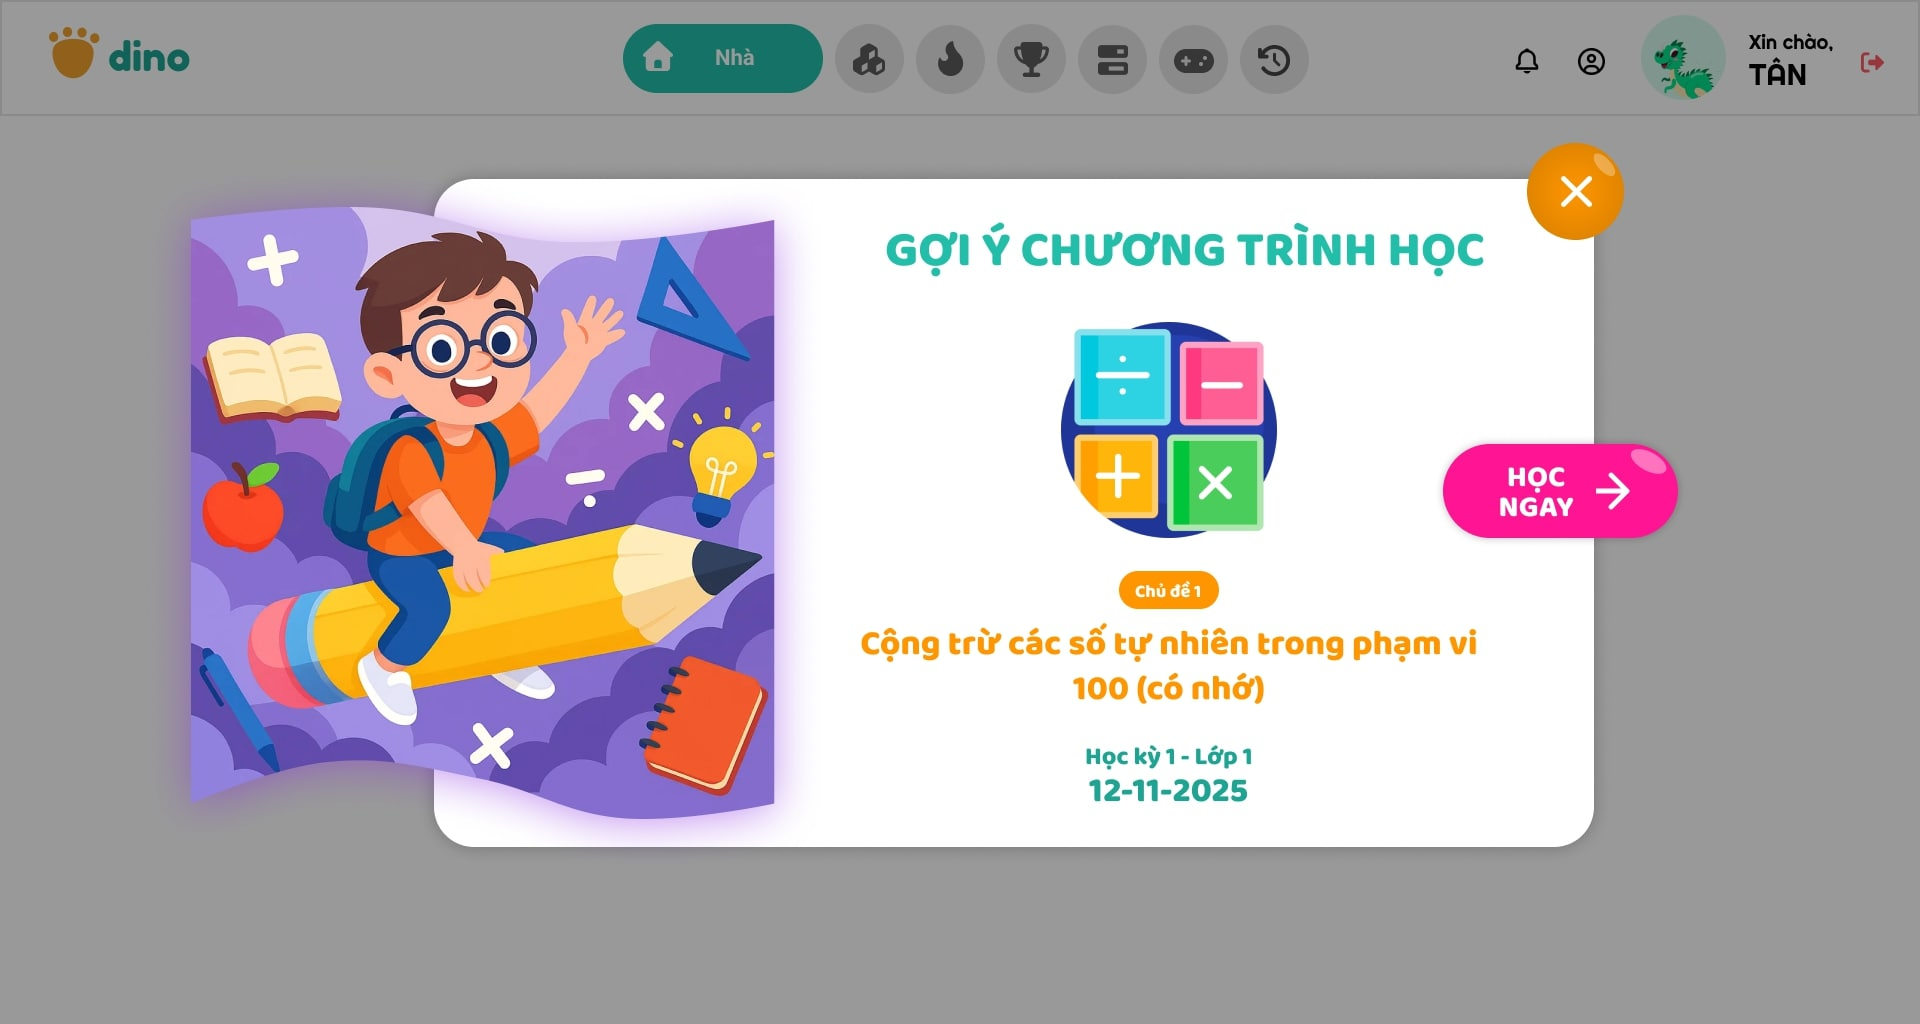
\includegraphics[width=0.9\textwidth]{Image/UI/Main-Student/LessonRecommend.jpg}
		\vspace{0.6cm}
		\caption{Trang chủ - Gợi ý chủ đề học}
		\label{fig:recommend}
	\end{figure}

\vspace{0.2cm}
\newline
Đối với người dùng mới, hệ thống sẽ hiển thị thông báo về bài kiểm tra đầu vào dưới dạng popup được thiết kế như \textit{Hình \ref{fig:enttest}}. Người dùng có thể bấm vào nút \textit{Làm bài} để điều hướng đến giao diện bài kiểm tra được mô tả chi tiết ở mục \ref{subsubsec:exam}, hoặc bấm vào nút \textit{Đóng} để đóng popup. Sau khi đóng, người dùng có thể mở lại popup này bằng cách bấm vào float button hiển thị ở góc phải trên cùng của giao diện trang chủ như \textit{Hình \ref{fig:floatbtn}}.
	\begin{figure}[H]
		\centering
		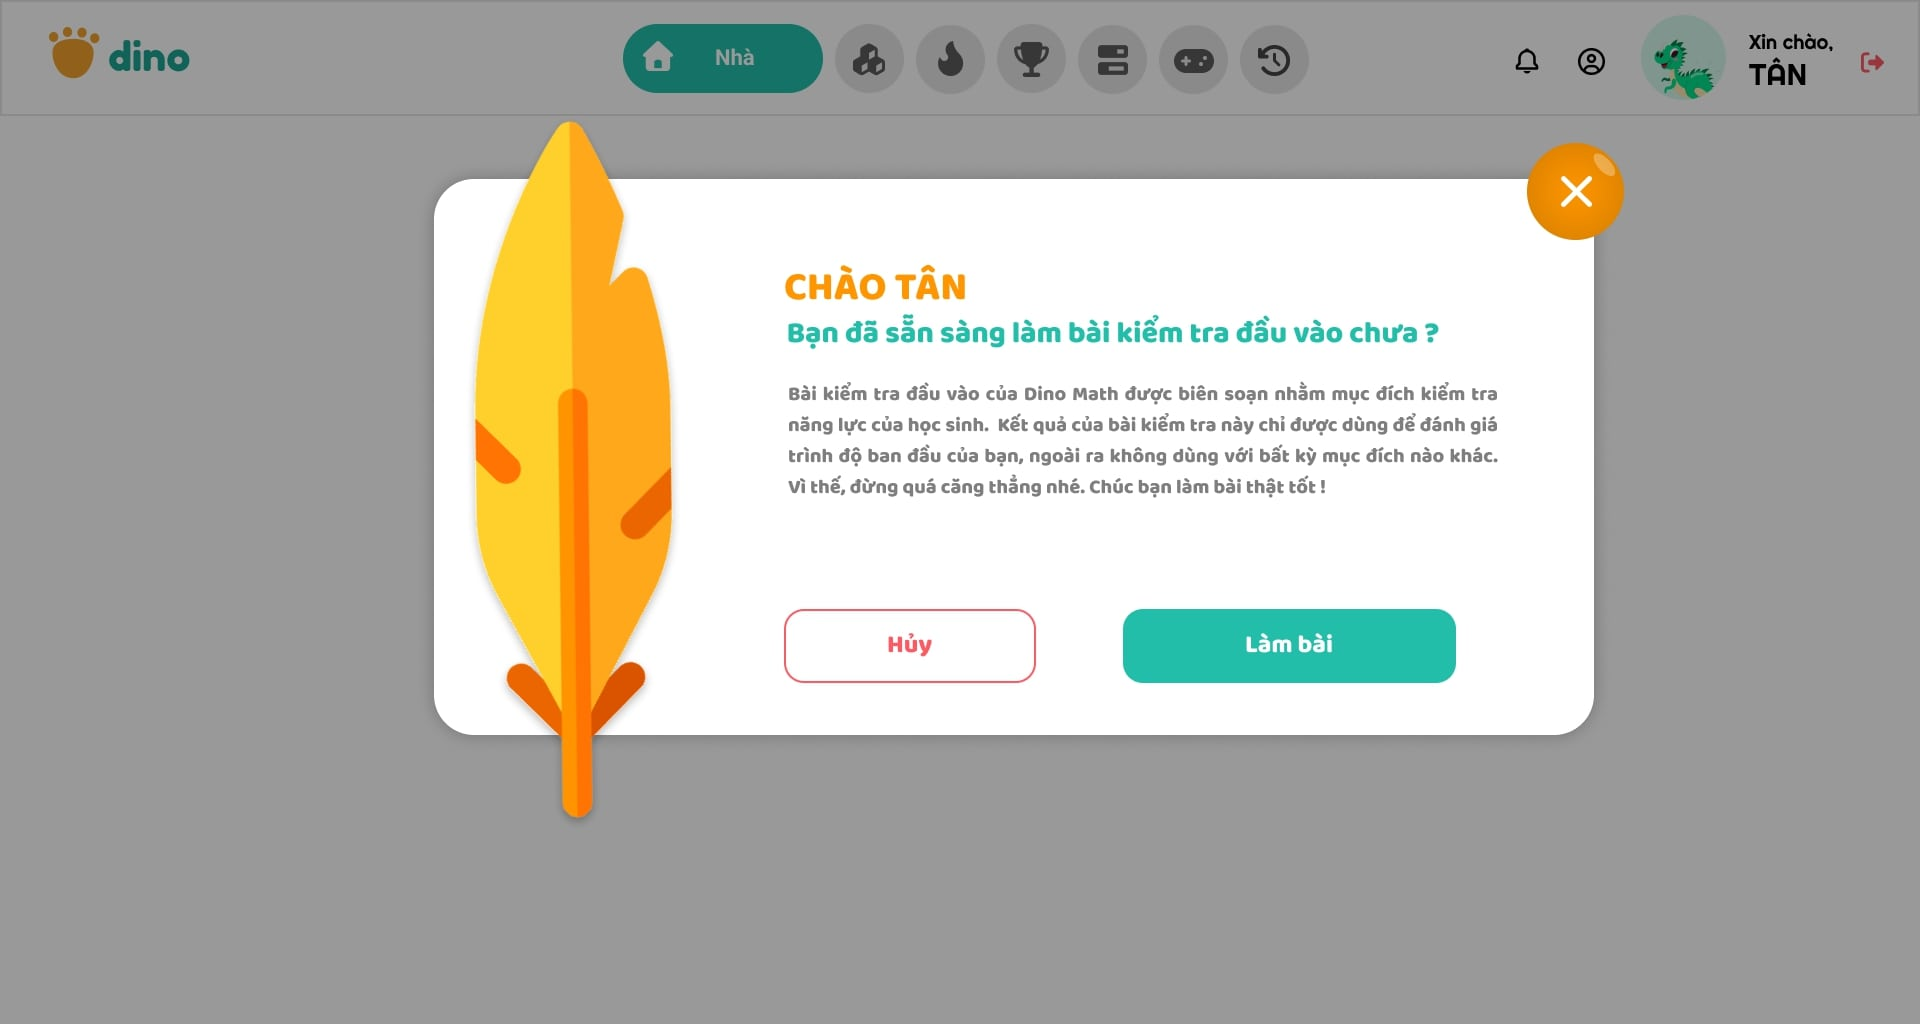
\includegraphics[width=0.9\textwidth]{Image/UI/Main-Student/EntranceTestPopup.jpg}
		\vspace{0.6cm}
		\caption{Trang chủ - Popup thông báo về bài kiểm tra đầu vào}
		\label{fig:enttest}
	\end{figure}
	\begin{figure}[H]
		\centering
		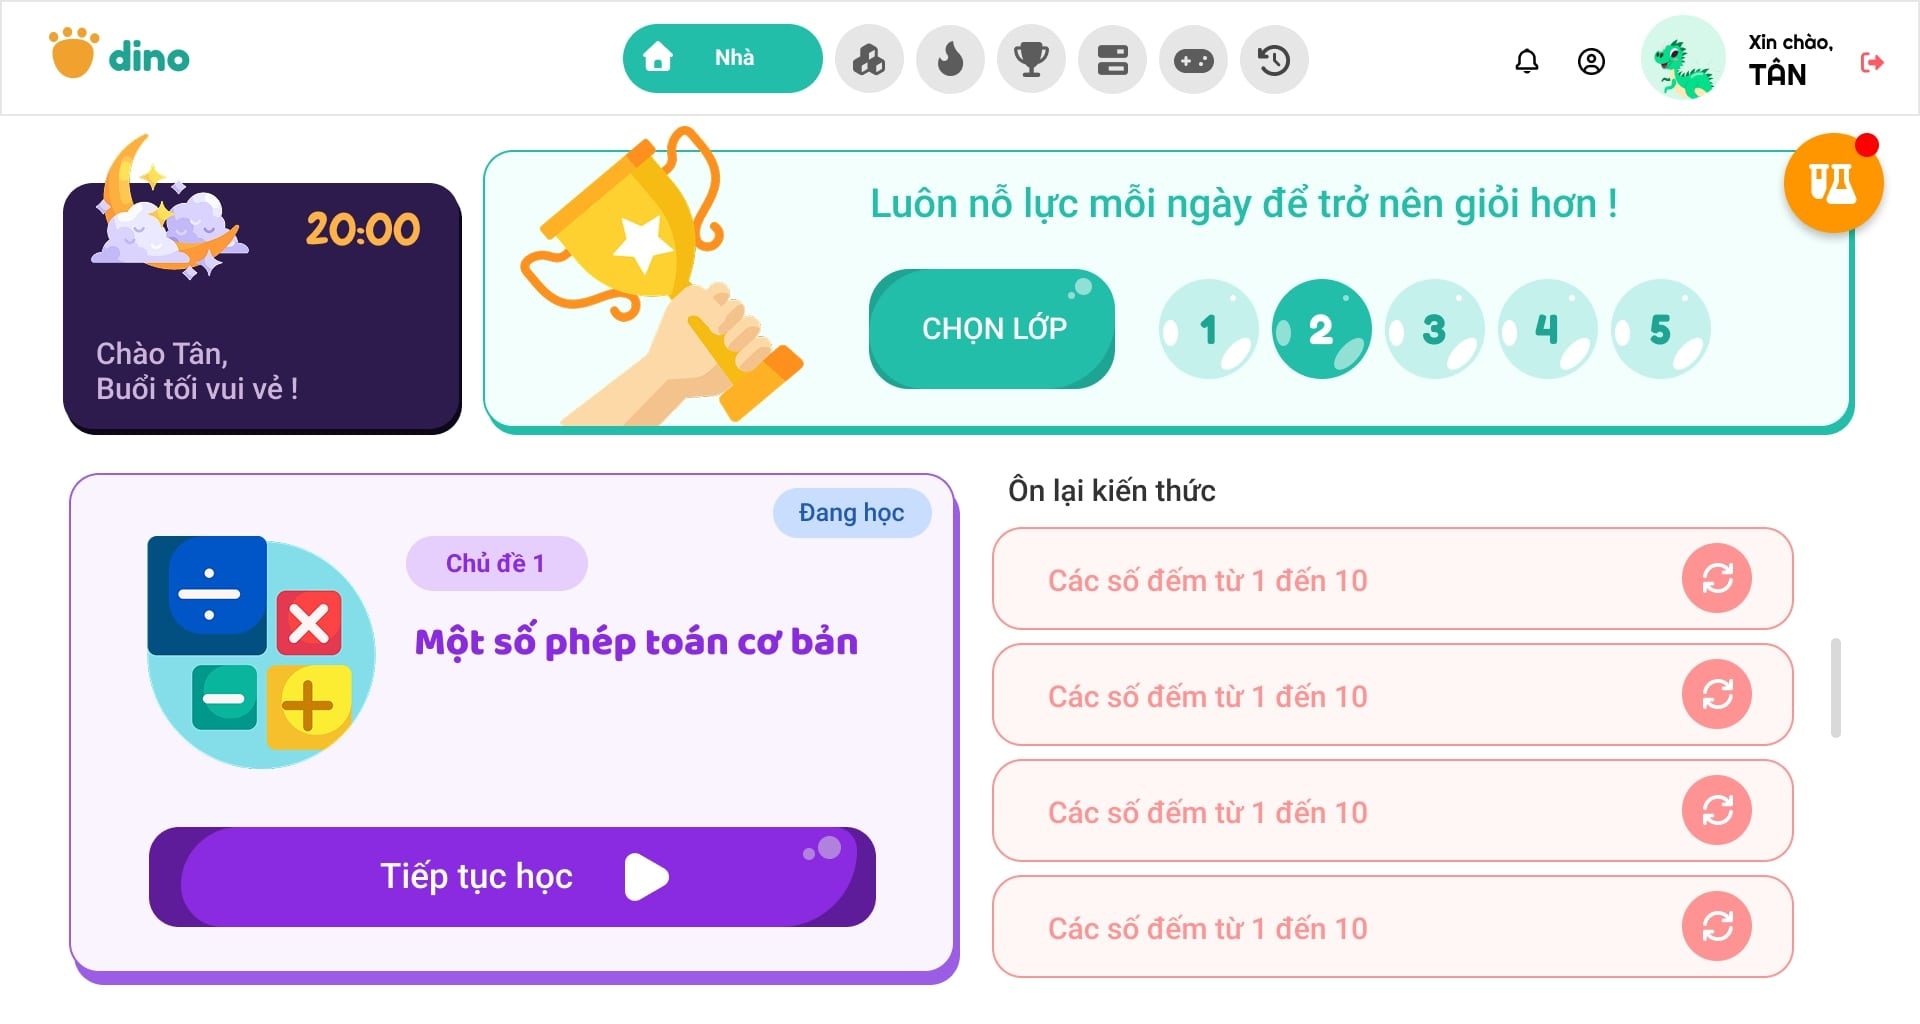
\includegraphics[width=0.9\textwidth]{Image/UI/Main-Student/EntranceTestFloatingButton.jpg}
		\vspace{0.6cm}
		\caption{Trang chủ - Nút mở popup bài kiểm tra đầu vào ở góc trên bên phải}
		\label{fig:floatbtn}
	\end{figure}


\subsubsection{Trang Bài học}
\label{subsubsec:lesson}
Phần nội dung chính của trang Bài học liệt kê danh sách toàn bộ các chủ đề thuộc khối lớp hiện tại, bao gồm cả những chủ đề đã được mở khóa (như minh họa tại \textit{Hình \ref{fig:lesson}}) và các chủ đề còn đang trong trạng thái khóa (như minh họa tại \textit{Hình \ref{fig:lessonlocked}}). Để bắt đầu quá trình học, người dùng có thể nhấn vào các thẻ chủ đề trong danh sách. Bên cạnh đó, người dùng cũng có thể nhanh chóng quay lại nội dung đang học dang dở bằng cách nhấn nút \textit{Bắt đầu} nằm trong container chủ đề được bố trí phía trên danh sách. Cả 2 thao tác kể trên đều sẽ điều hướng người dùng đến \textbf{Trang Chủ đề} được mô tả ở mục \ref{subsubsec:topic}.

\begin{figure}[H]
	\centering
	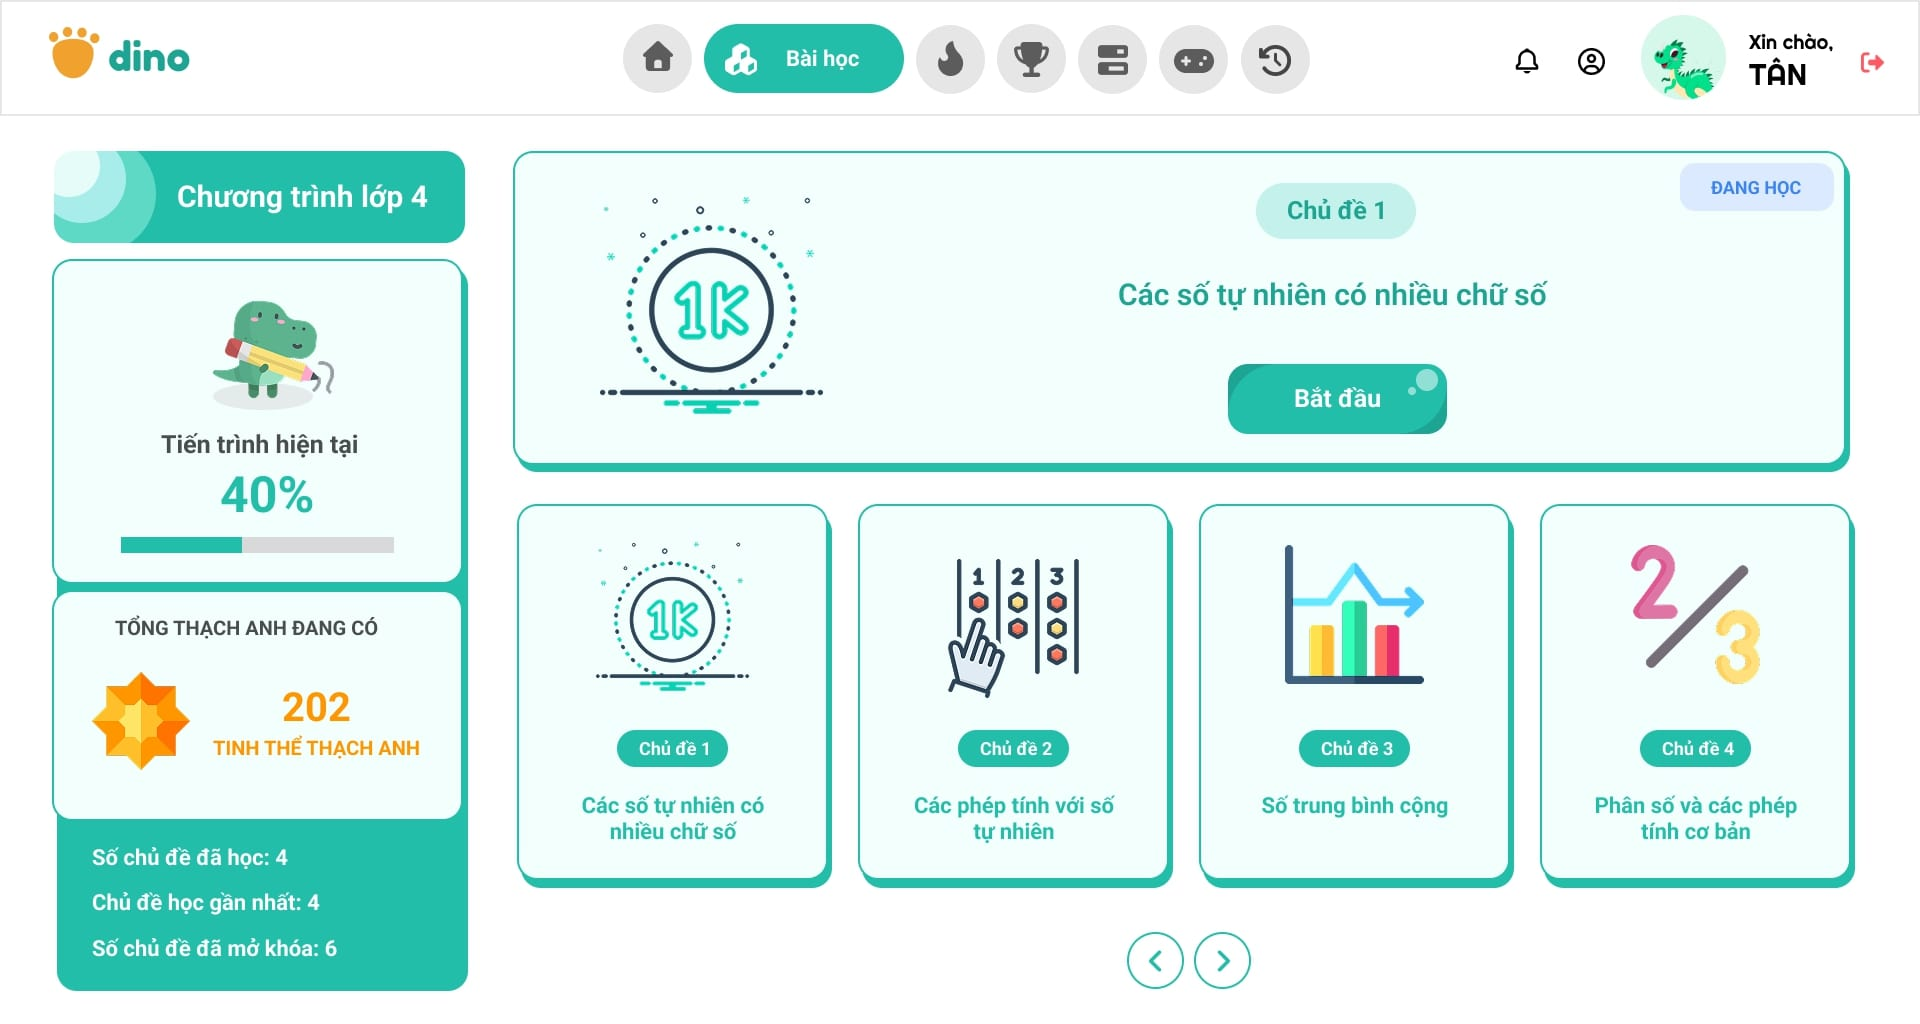
\includegraphics[width=0.9\textwidth]{Image/UI/Main-Student/Topics-G4.jpg}
	\vspace{0.6cm}
	\caption{Trang Bài học - Các chủ đề của Lớp 4 (tương tự với các lớp khác)}
	\label{fig:lesson}
\end{figure}
\begin{figure}[H]
	\centering
	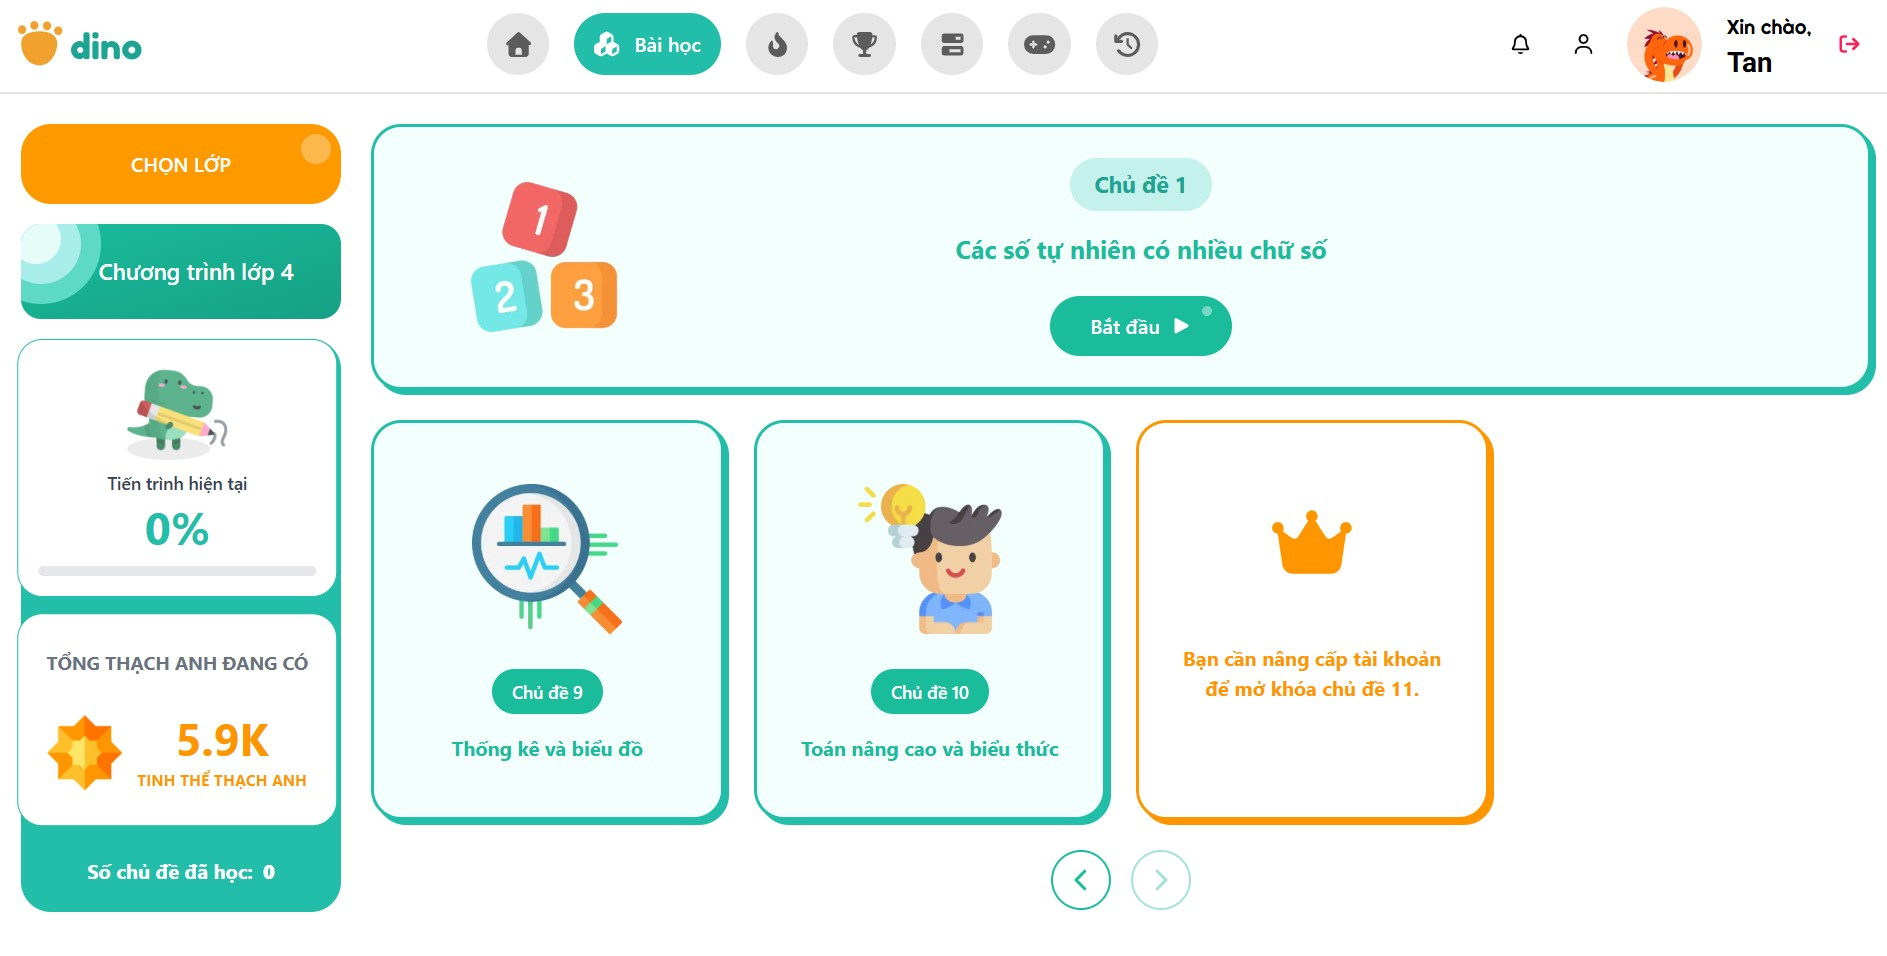
\includegraphics[width=0.9\textwidth]{Image/UI/Main-Student/PremiumTopic.jpg}
	\vspace{0.6cm}
	\caption{Trang Bài học - Các chủ đề bị khóa}
	\label{fig:lessonlocked}
\end{figure}

\vspace{0.2cm}
\newline
Ngoài liệt kê danh sách các bài học, hệ thống còn hiển thị rõ ràng thông tin về khối lớp hiện tại mà học sinh đã lựa chọn ở \textbf{Trang chủ} (được mô tả chi tiết trong mục \ref{subsubsec:studenthome}). Đi kèm với đó, hệ thống sẽ cập nhật tiến trình học tập hiện tại thông qua tỉ lệ phần trăm các chủ đề đã hoàn thành trên tổng số chủ đề thuộc khối lớp đó. Ngoài ra, tổng số lượng Thạch anh tích lũy được từ các hoạt động học tập cũng được hiển thị đầy đủ, đóng vai trò như một hệ thống điểm thưởng để xếp hạng người dùng. Hệ thống cũng cung cấp các số liệu thống kê cụ thể bao gồm số lượng chủ đề đã học, số lượng chủ đề đã mở khóa và thông tin về chủ đề gần nhất mà người dùng vừa truy cập.

\subsubsection{Trang Chủ đề (Trang Milestones)}
\label{subsubsec:topic}
\textbf{Trang Chủ đề} chỉ có thể truy cập bằng cách bấm vào các thẻ chủ đề ở \textbf{Trang Bài học} trong mục \ref{subsubsec:lesson} hoặc bấm vào các nút \textit{Tiếp tục học/Bắt đầu} trong container hiển thị chủ đề học gần nhất được mô tả ở \textbf{Trang chủ} (mục \ref{subsubsec:studenthome}) và \textbf{Trang Bài học} (mục \ref{subsubsec:lesson}). Nhóm thiết kế giao diện cho \textbf{Trang Chủ đề} theo phong cách phiêu lưu qua từng thế giới và vùng đất, tạo cho người dùng cảm giác hứng thú với việc học tập. Mỗi khối lớp gắn liền với một thế giới khác nhau, mỗi thế giới lại gồm các vùng đất khác nhau ứng với các độ khó khác nhau. Trang còn bao gồm danh sách các milestone, mỗi milestone đóng vai trò như một bài học trong chủ đề bao gồm nhiều bài tập tương tác giúp học sinh luyện tập khả năng làm toán.

\vspace{0.2cm}
\newline
Ngoài ra, trang còn hiển thị tên chủ đề hiện tại cùng với tiến trình học tập (tỉ lệ phần trăm các milestone đã học trên tổng số milestone của chủ đề đó). Người dùng phải học hết các milestone thuộc một độ khó nhất định thì mới mở khóa được các milestone ở độ khó tiếp theo. Người dùng có thể bấm vào nút mũi tên ở 2 bên chuyển đổi giữa các milestone, sau đó bấm nút \textit{Làm bài nào !} để điều hướng sang \textbf{Trang Bài tập} được mô tả ở mục \ref{subsubsec:exercise}. 

\newpage
	% --- Trang Chủ đề của Lớp 1 ---
	\noindent Thế giới của Lớp 1 được thiết kế với bối cảnh thảo nguyên do đây là lớp nhỏ nhất và có độ khó thấp nhất. Các hình từ \ref{fig:e1} đến \ref{fig:h1} là thiết kế cho trang chủ đề của lớp 1 ứng với các mức độ khó khác nhau của bài học. Giao diện khóa của các bài học (milestone) được thiết kế như \textit{Hình \ref{fig:l1}}.
	\begin{figure}[H]
		\centering
		\begin{minipage}{0.45\textwidth}
			\centering
			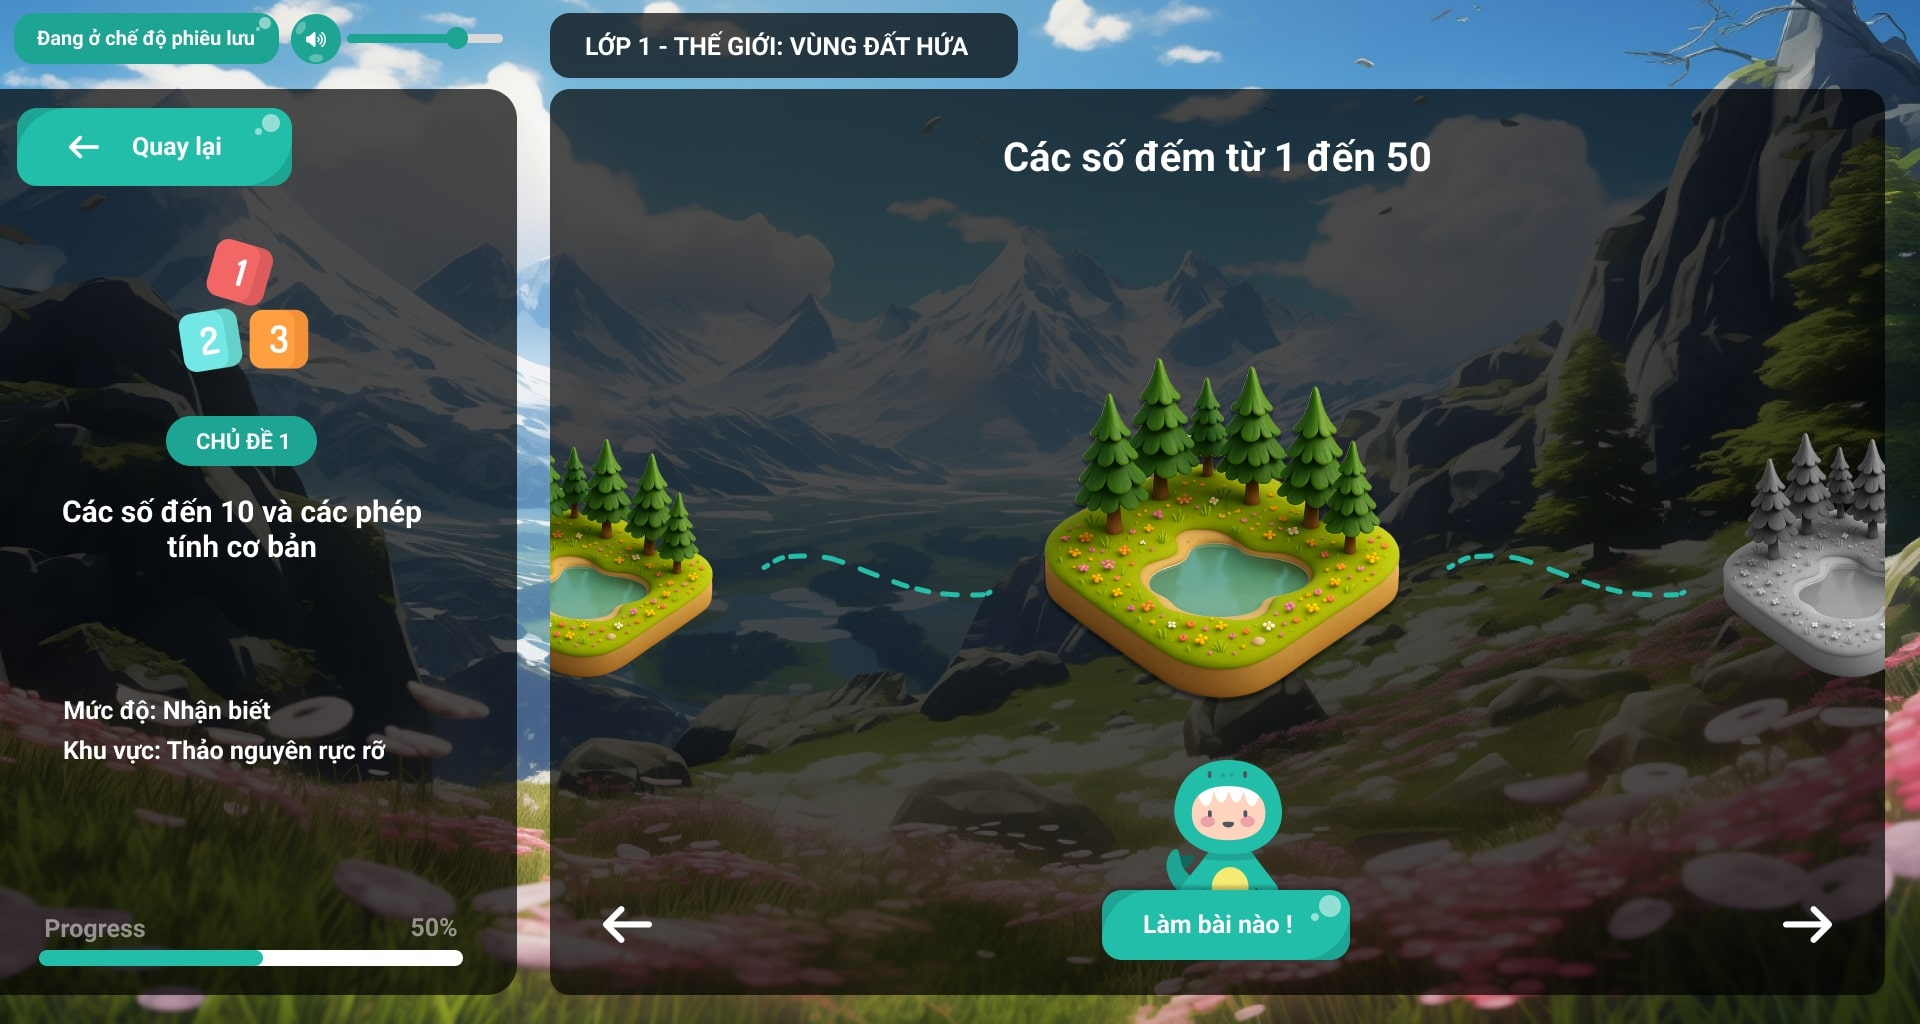
\includegraphics[width=\textwidth]{Image/UI/Milestones/Paths-G1-NB.jpg}
			\vspace{0.2cm}
			\caption{Lớp 1 - Nhận biết}
			\label{fig:e1}
		\end{minipage}
		\hspace{0.1cm}
		\begin{minipage}{0.45\textwidth}
			\centering
			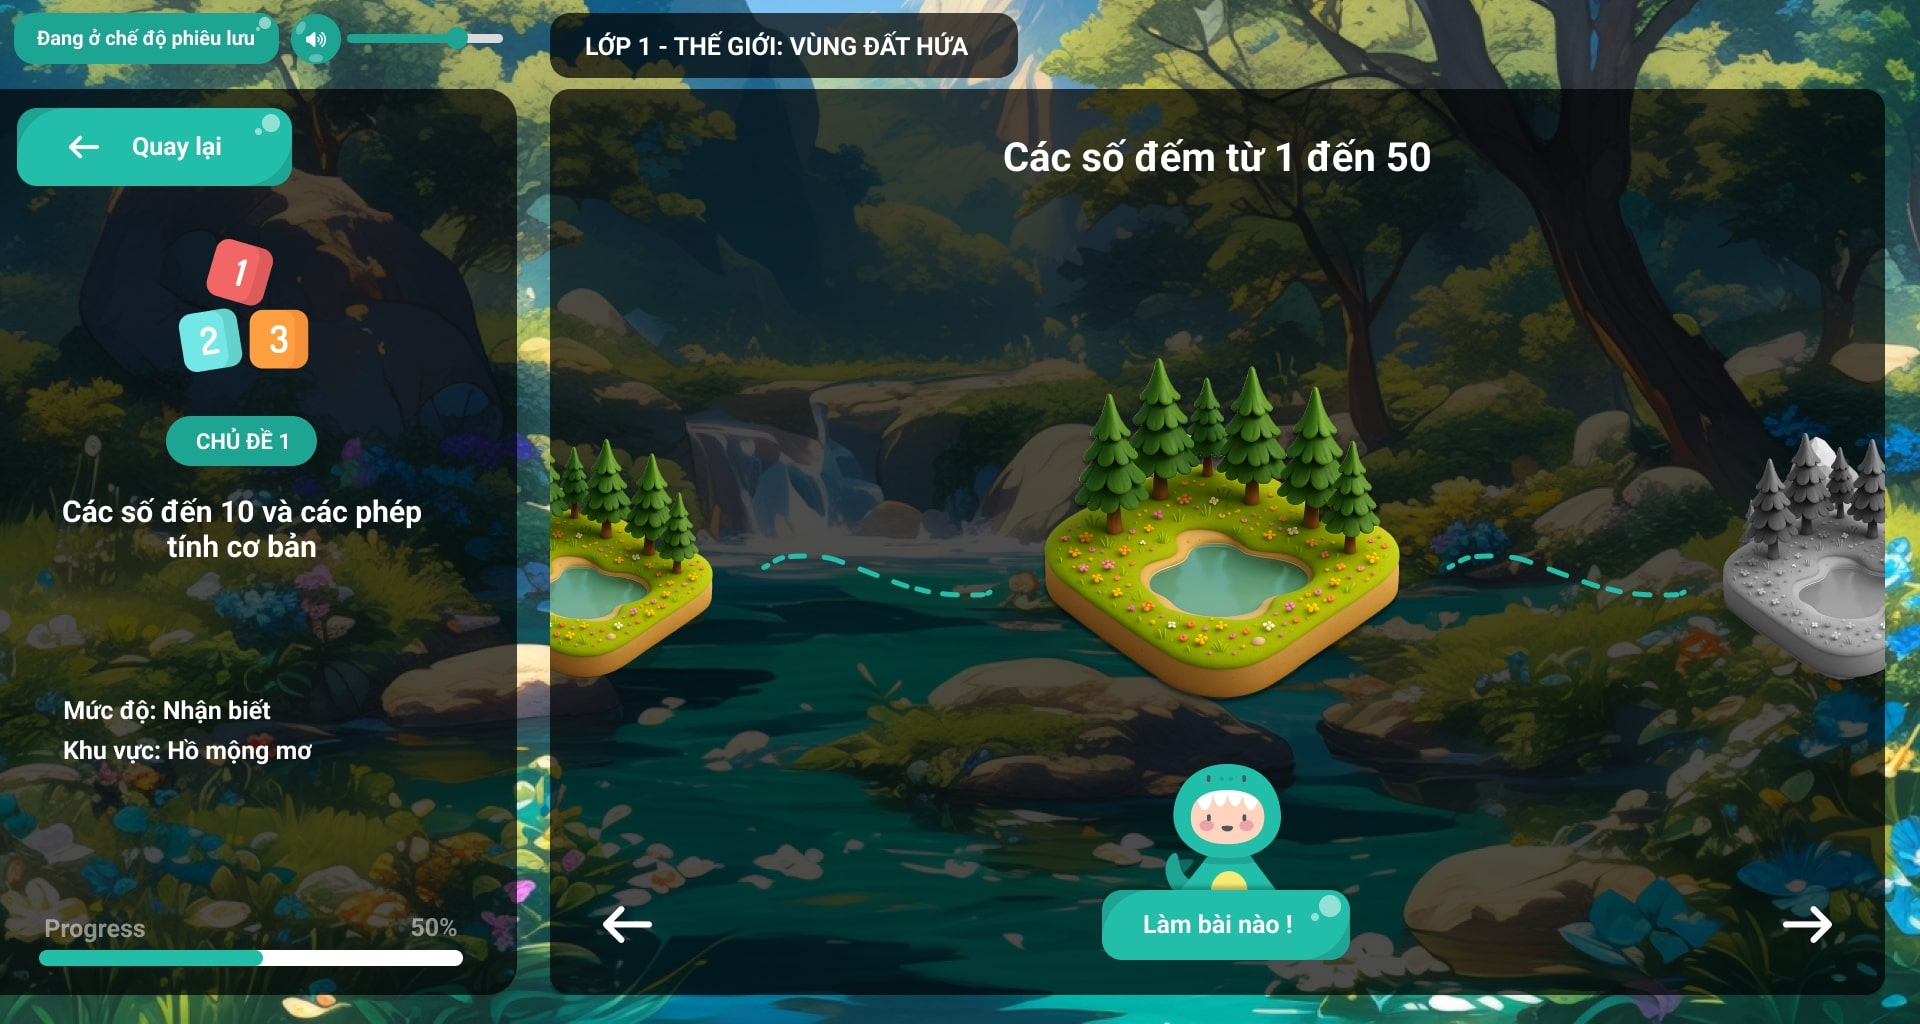
\includegraphics[width=\textwidth]{Image/UI/Milestones/Paths-G1-TH.jpg}
			\vspace{0.2cm}
			\caption{Lớp 1 - Thông hiểu}
			\label{fig:md1}
		\end{minipage}
		
		\vspace{0.4cm}
		
		\begin{minipage}{0.45\textwidth}
			\centering
			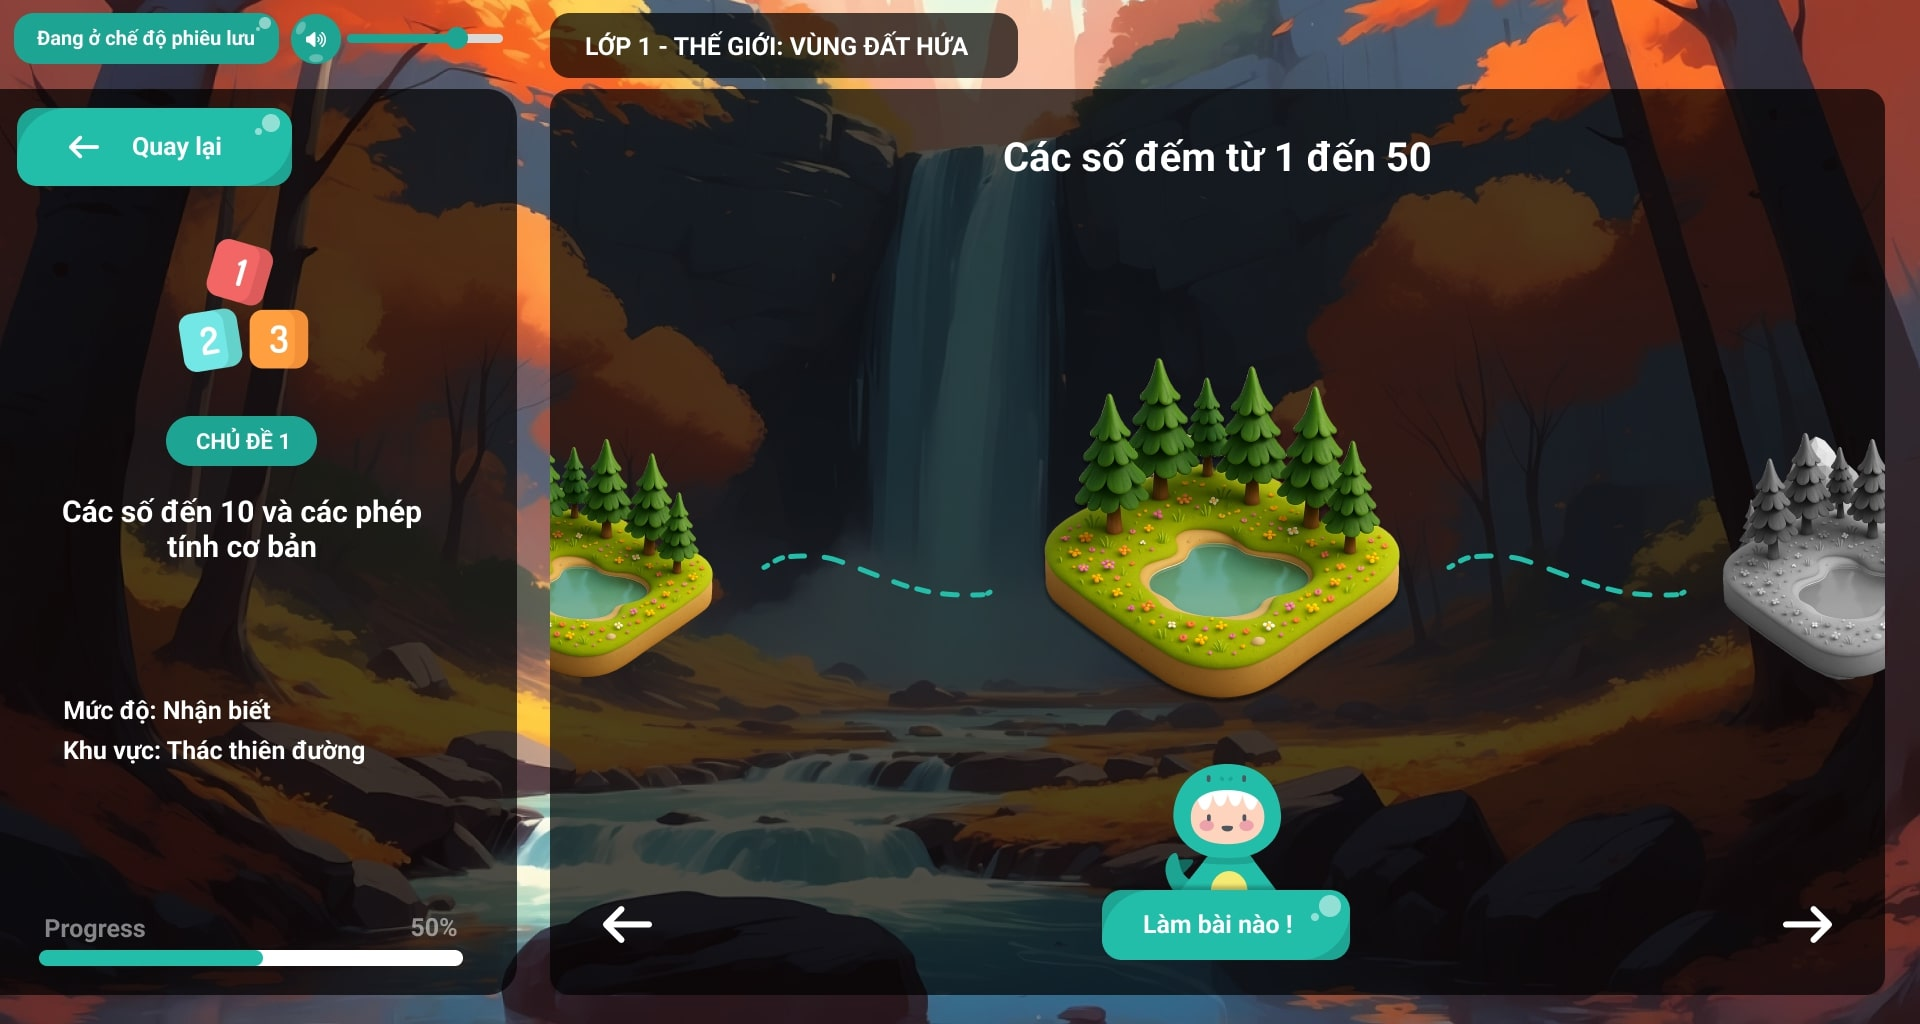
\includegraphics[width=\textwidth]{Image/UI/Milestones/Paths-G1-VD.jpg}
			\vspace{0.2cm}
			\caption{Lớp 1 - Vận dụng}
			\label{fig:h1}
		\end{minipage}
		\hspace{0.1cm}
		\begin{minipage}{0.45\textwidth}
			\centering
			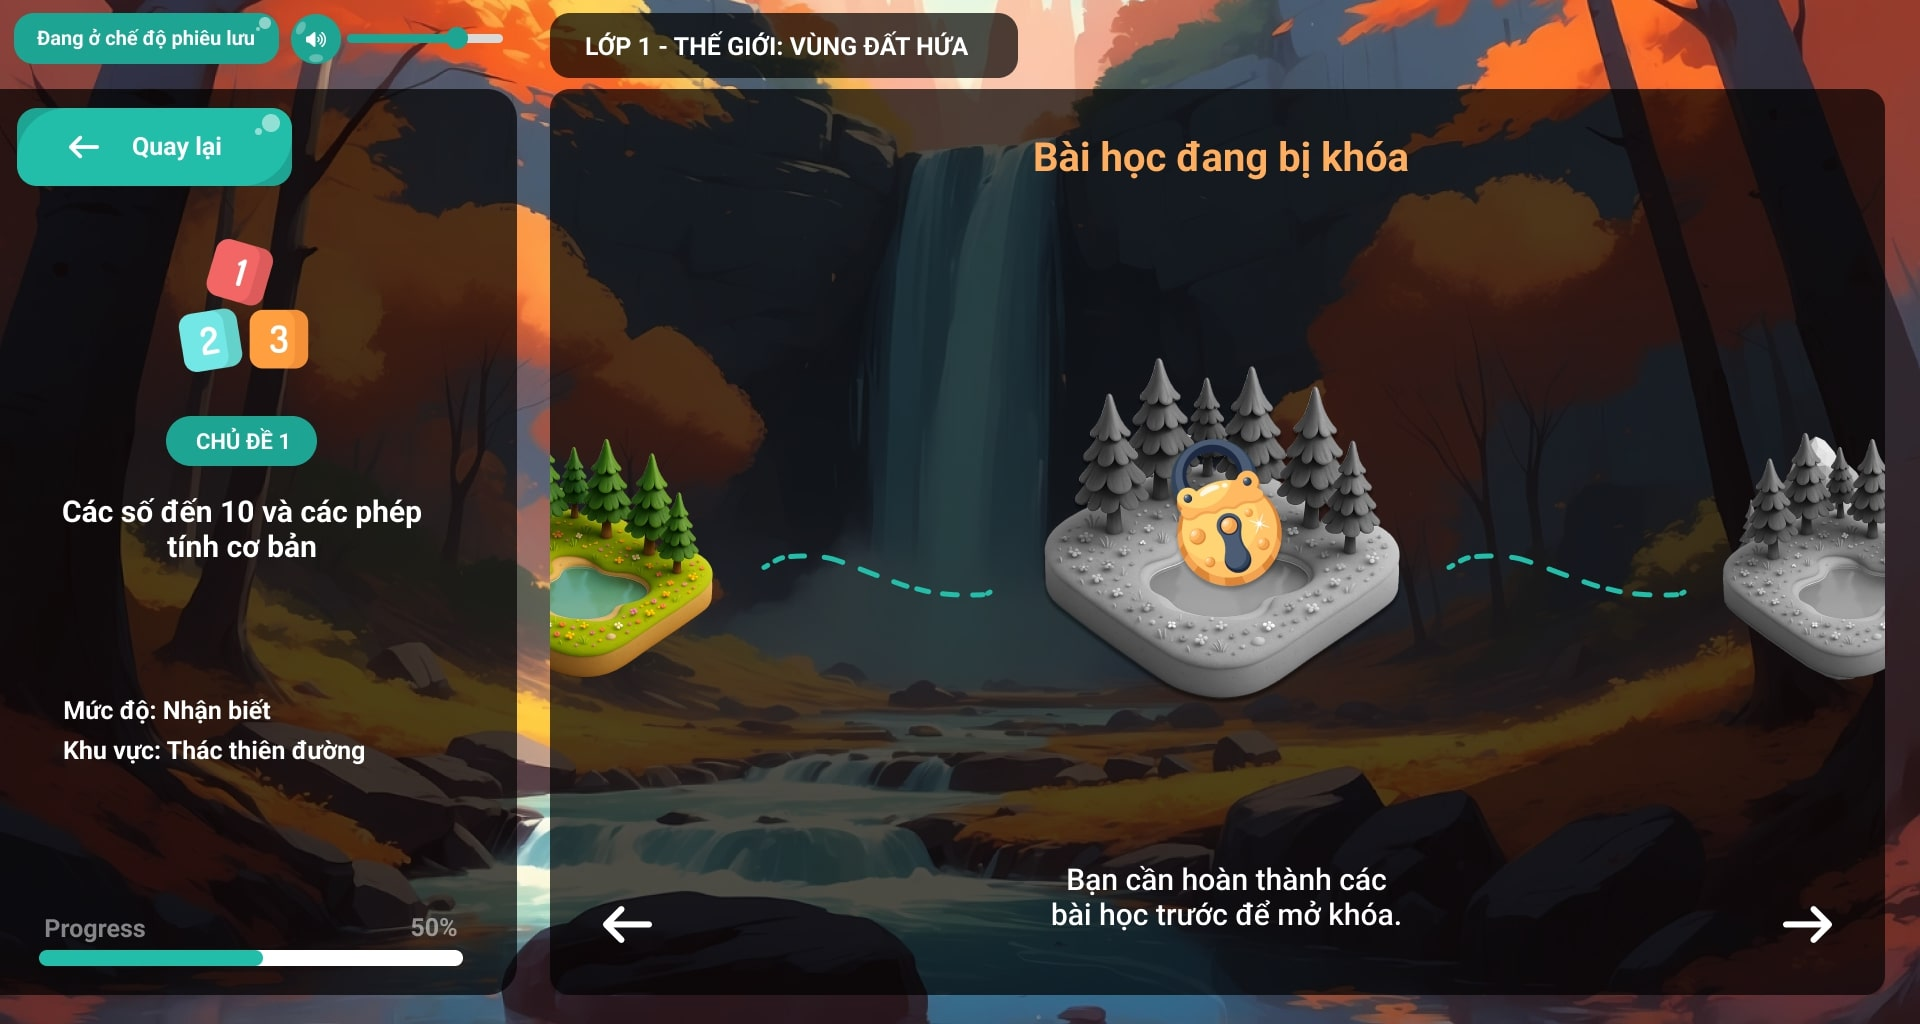
\includegraphics[width=\textwidth]{Image/UI/Milestones/Paths-G1-Locked.jpg}
			\vspace{0.2cm}
			\caption{Lớp 1 - Milestone bị khóa}
			\label{fig:l1}
		\end{minipage}
	\end{figure}
	
	\vspace{0.4cm}
	
	% --- Trang Chủ đề của Lớp 2 ---
	\noindent Thế giới của Lớp 2 được thiết kế với bối cảnh rừng rậm, khắc nghiệt hơn thảo nguyên một chút. Các hình từ \ref{fig:e2} đến \ref{fig:h2} là thiết kế cho trang chủ đề của lớp 2 ứng với các mức độ khó khác nhau của bài học. Giao diện khóa của các bài học (milestone) được thiết kế như \textit{Hình \ref{fig:l2}}.
	\begin{figure}[H]
		\centering
		\begin{minipage}{0.45\textwidth}
			\centering
			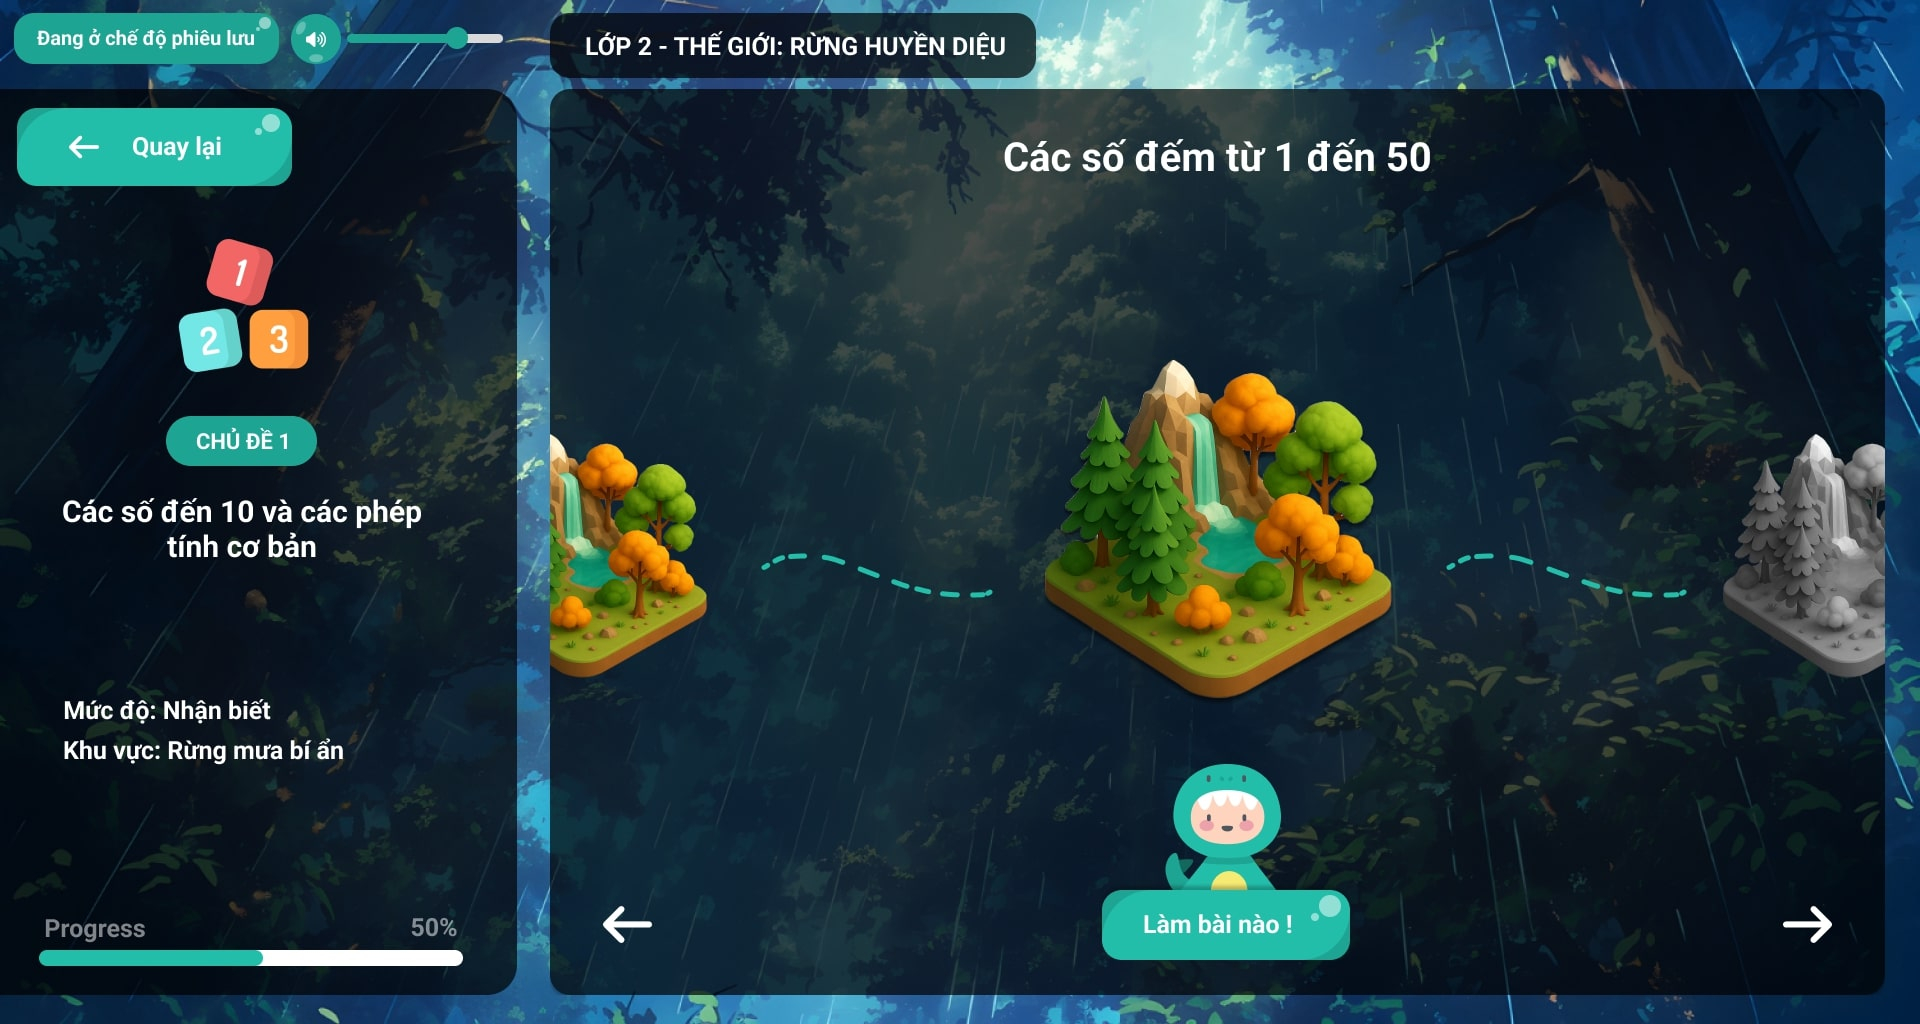
\includegraphics[width=\textwidth]{Image/UI/Milestones/Paths-G2-NB.jpg}
			\vspace{0.2cm}
			\caption{Lớp 2 - Nhận biết}
			\label{fig:e2}
		\end{minipage}
		\hspace{0.1cm}
		\begin{minipage}{0.45\textwidth}
			\centering
			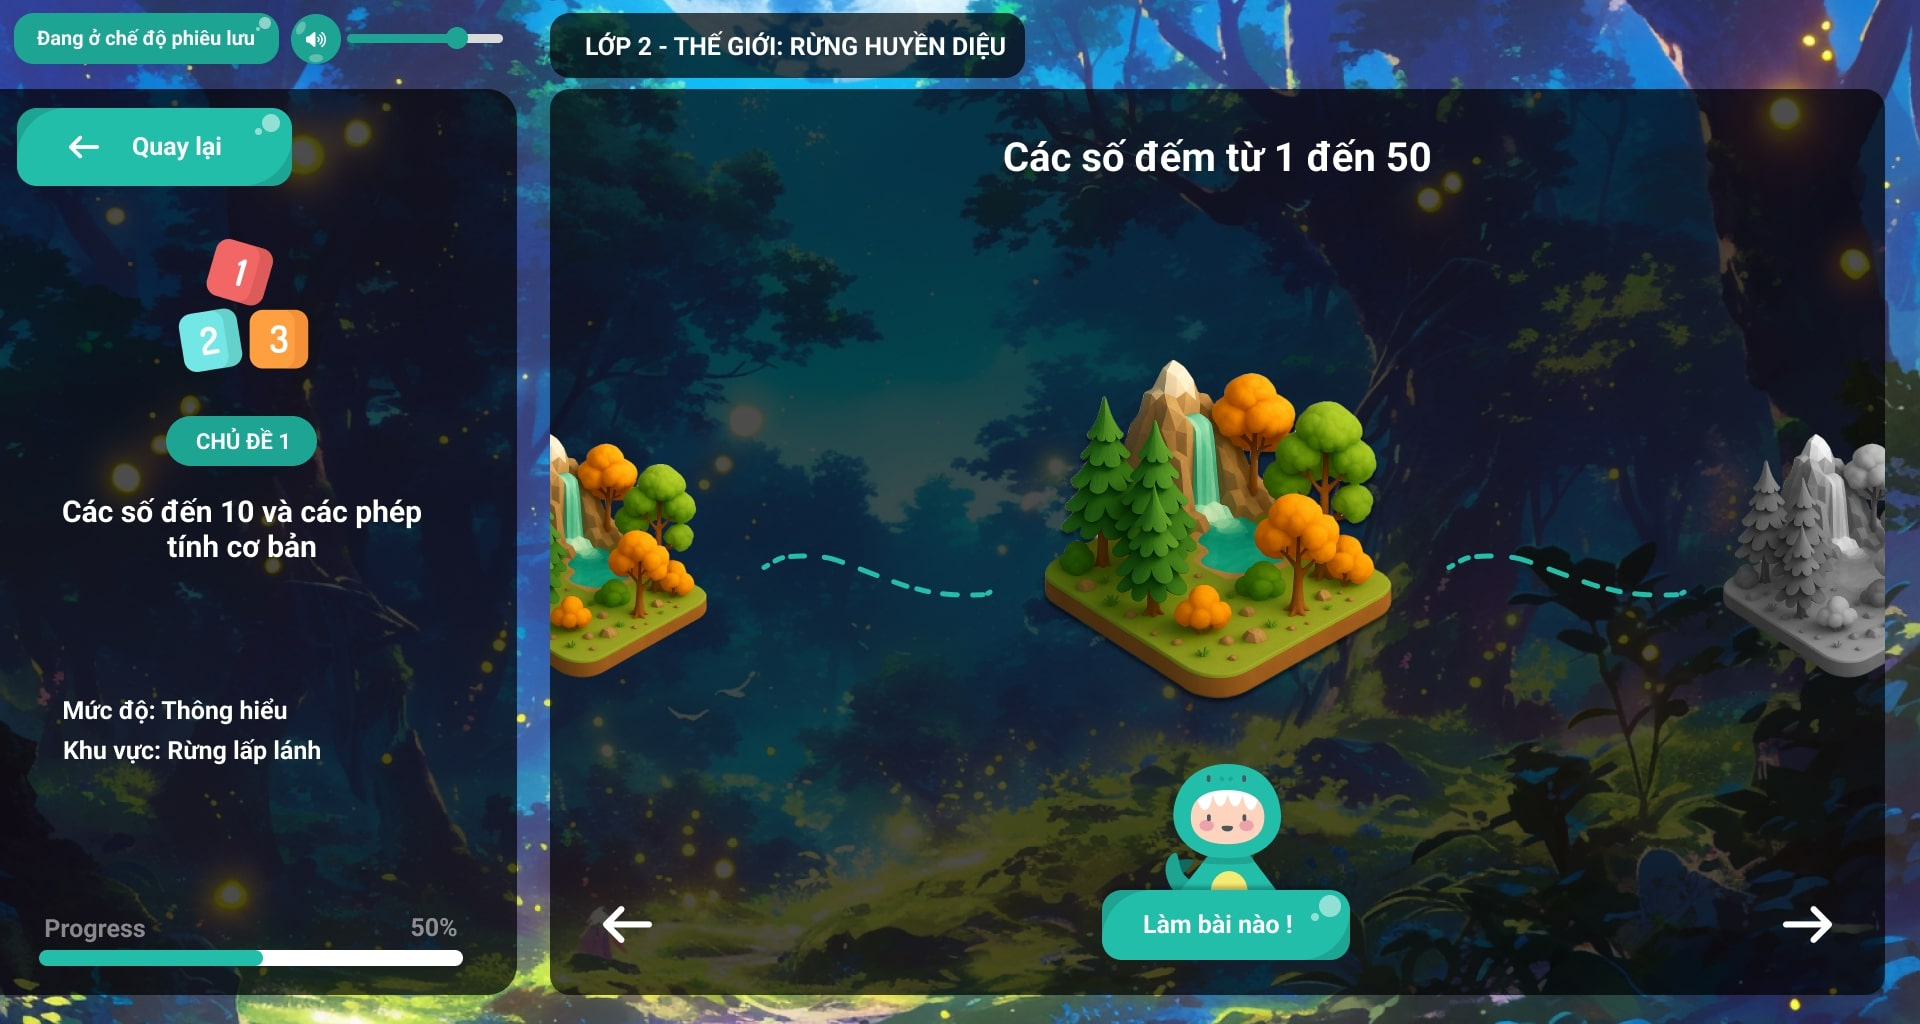
\includegraphics[width=\textwidth]{Image/UI/Milestones/Paths-G2-TH.jpg}
			\vspace{0.2cm}
			\caption{Lớp 2 - Thông hiểu}
			\label{fig:md2}
		\end{minipage}
		
		\vspace{0.4cm}
		
		\begin{minipage}{0.45\textwidth}
			\centering
			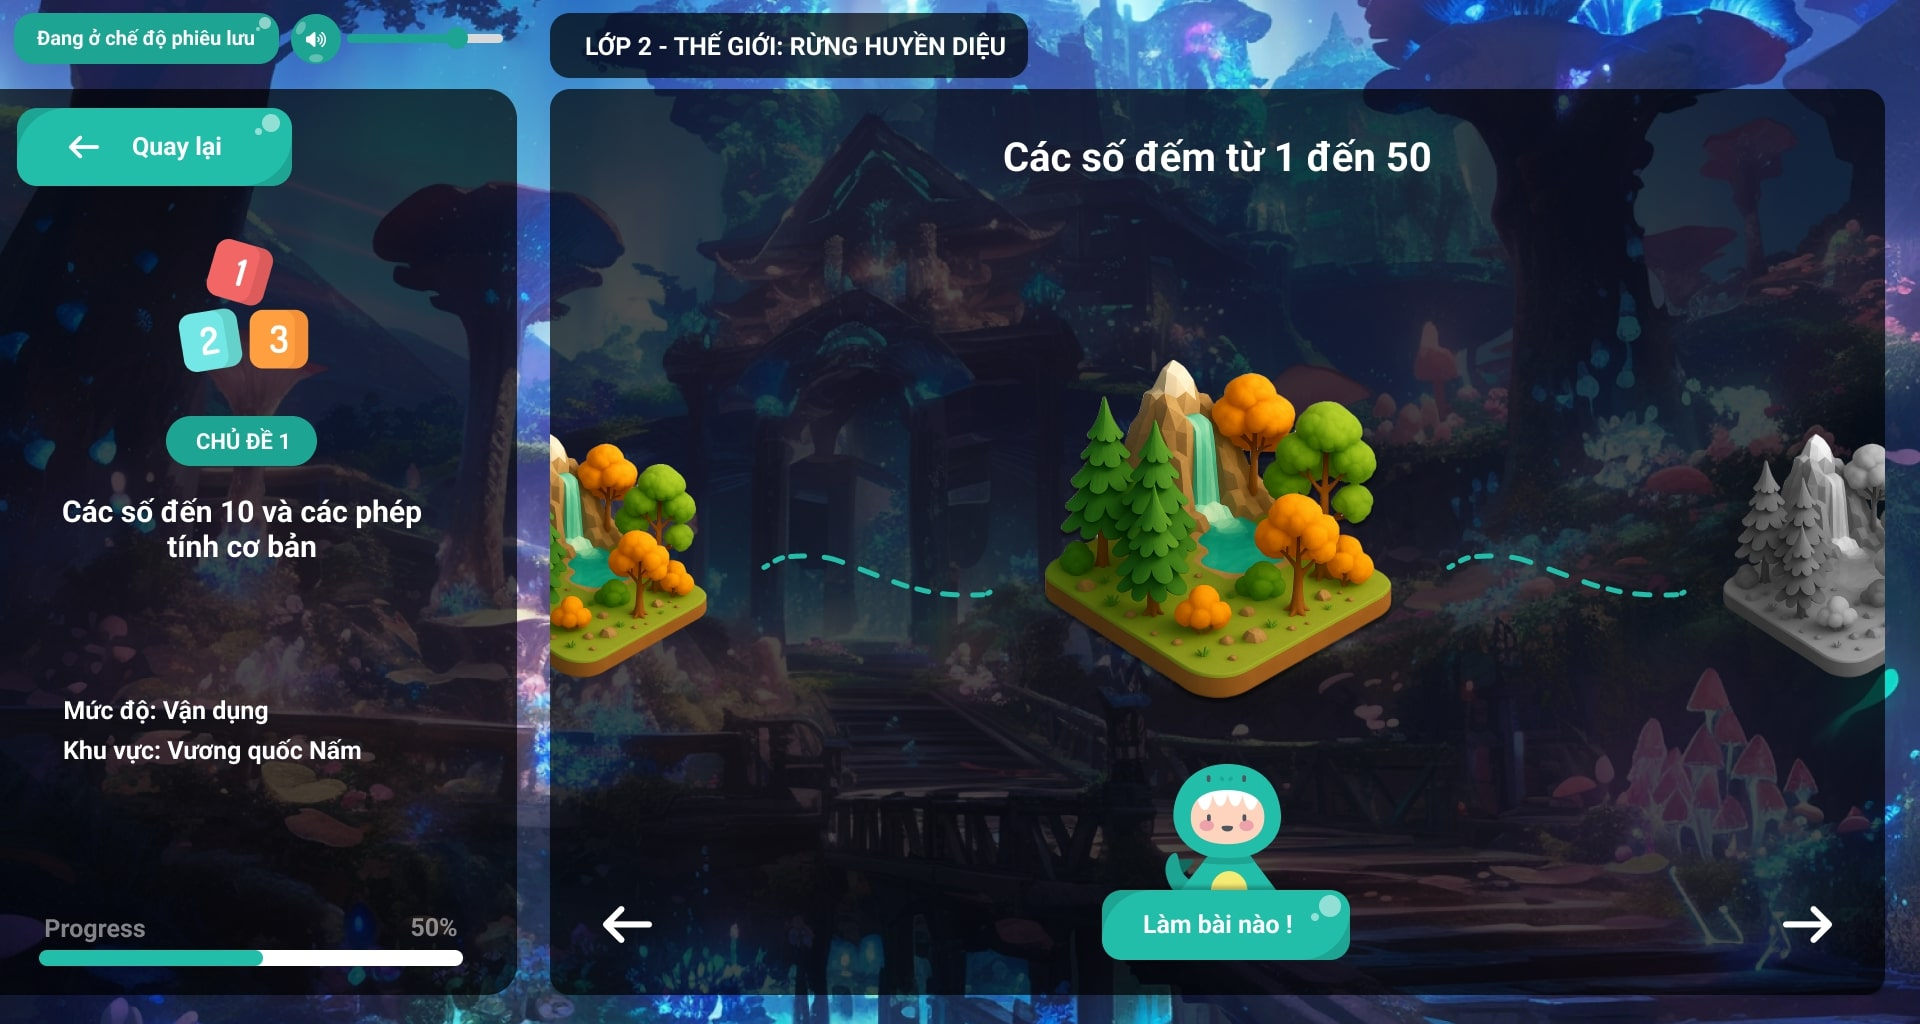
\includegraphics[width=\textwidth]{Image/UI/Milestones/Paths-G2-VD.jpg}
			\vspace{0.2cm}
			\caption{Lớp 2 - Vận dụng}
			\label{fig:h2}
		\end{minipage}
		\hspace{0.1cm}
		\begin{minipage}{0.45\textwidth}
			\centering
			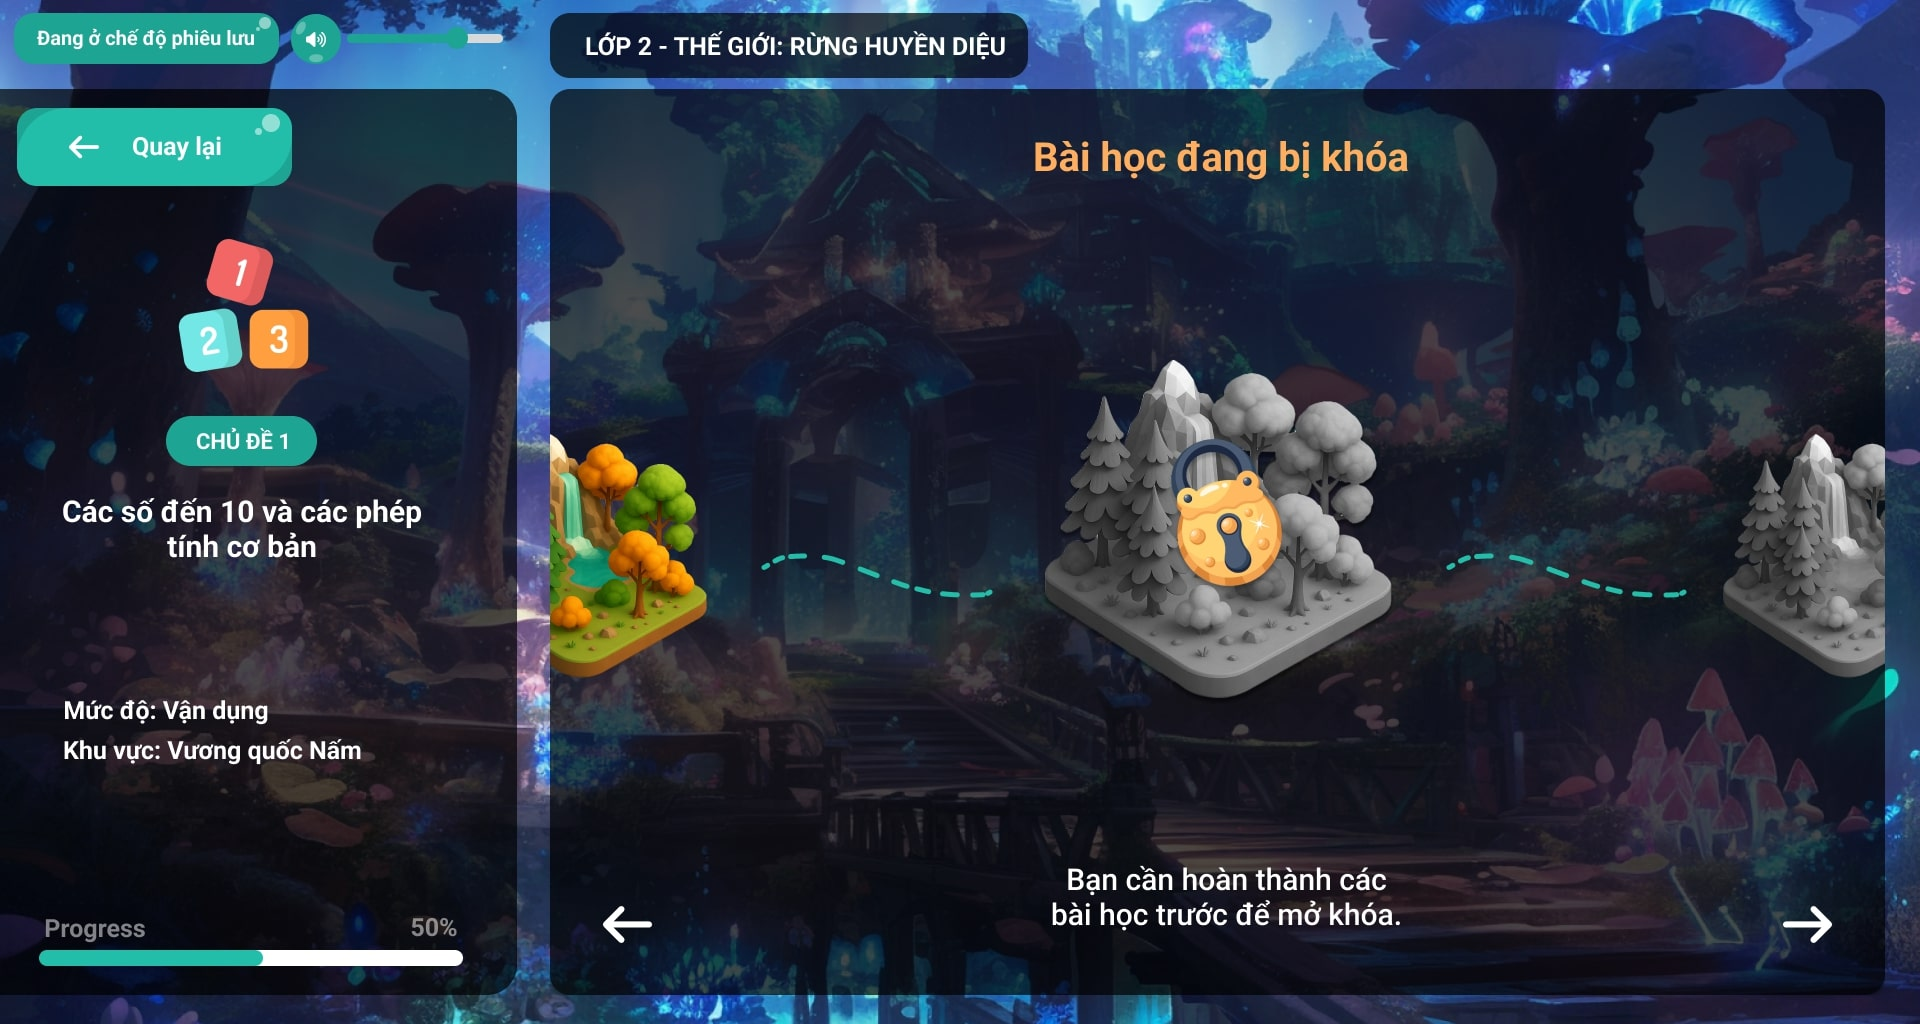
\includegraphics[width=\textwidth]{Image/UI/Milestones/Paths-G2-Locked.jpg}
			\vspace{0.2cm}
			\caption{Lớp 2 - Milestone bị khóa}
			\label{fig:l2}
		\end{minipage}
	\end{figure}
	
	\vspace{0.4cm}
	
	% --- Trang Chủ đề của Lớp 3 ---
	\noindent Thế giới của Lớp 3 được thiết kế với bối cảnh biển cả. Các hình từ \ref{fig:e3} đến \ref{fig:h3} là thiết kế cho trang chủ đề của lớp 3 ứng với các mức độ khó khác nhau của bài học. Giao diện khóa của các bài học (milestone) được thiết kế như \textit{Hình \ref{fig:l3}}.
	\begin{figure}[H]
		\centering
		\begin{minipage}{0.45\textwidth}
			\centering
			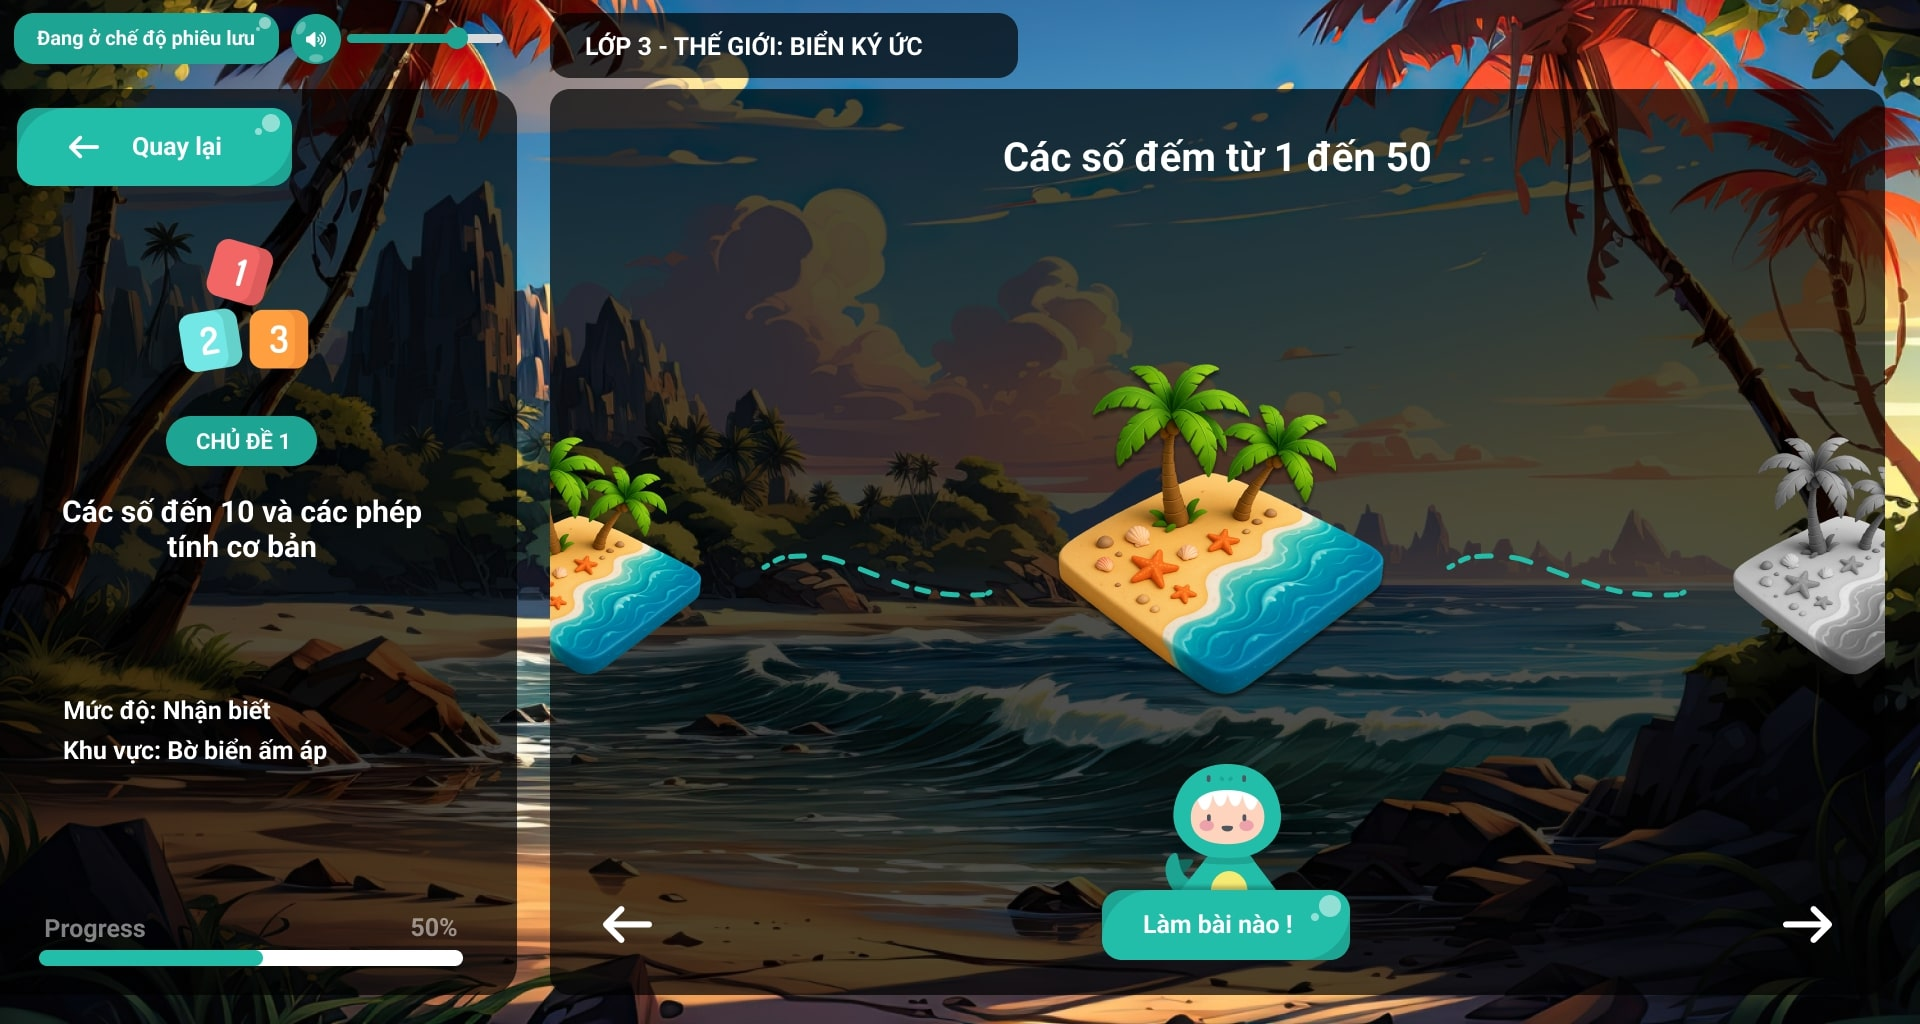
\includegraphics[width=\textwidth]{Image/UI/Milestones/Paths-G3-NB.jpg}
			\vspace{0.2cm}
			\caption{Lớp 3 - Nhận biết}
			\label{fig:e3}
		\end{minipage}
		\hspace{0.1cm}
		\begin{minipage}{0.45\textwidth}
			\centering
			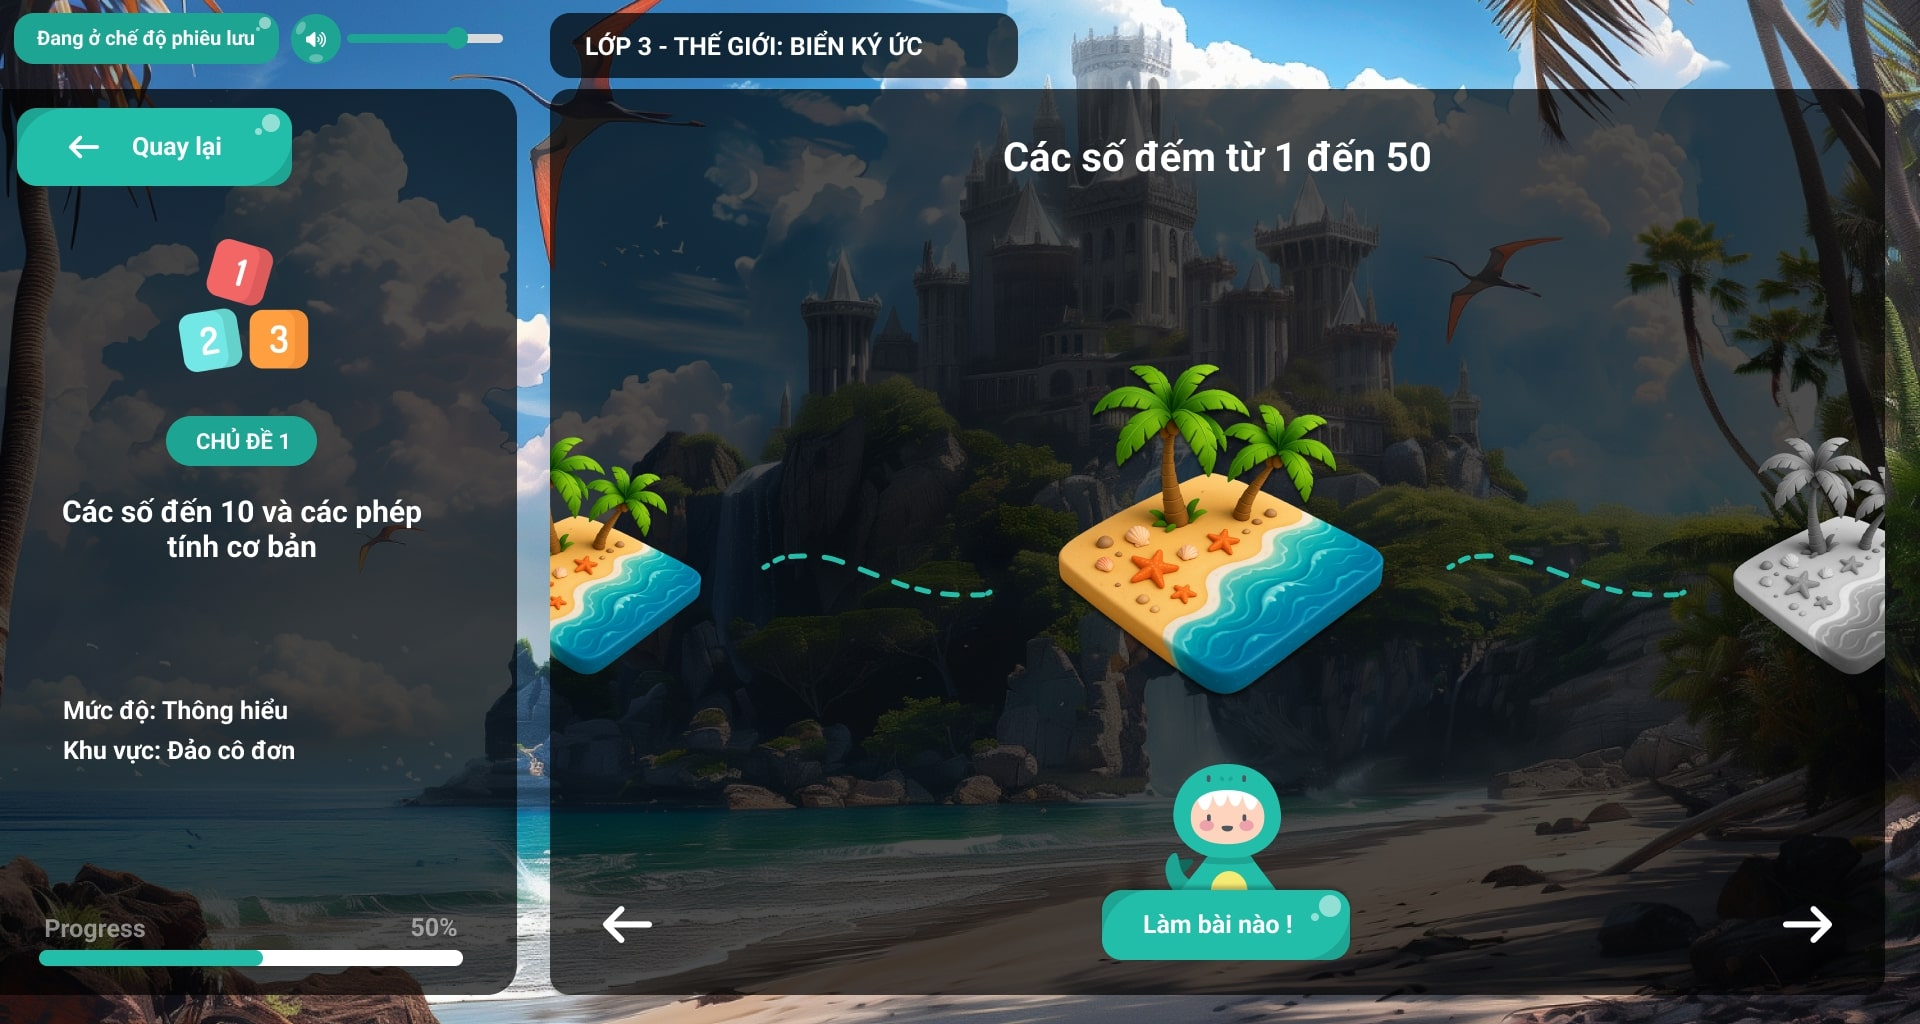
\includegraphics[width=\textwidth]{Image/UI/Milestones/Paths-G3-TH.jpg}
			\vspace{0.2cm}
			\caption{Lớp 3 - Thông hiểu}
		\end{minipage}
		
		\vspace{0.4cm}
		
		\begin{minipage}{0.45\textwidth}
			\centering
			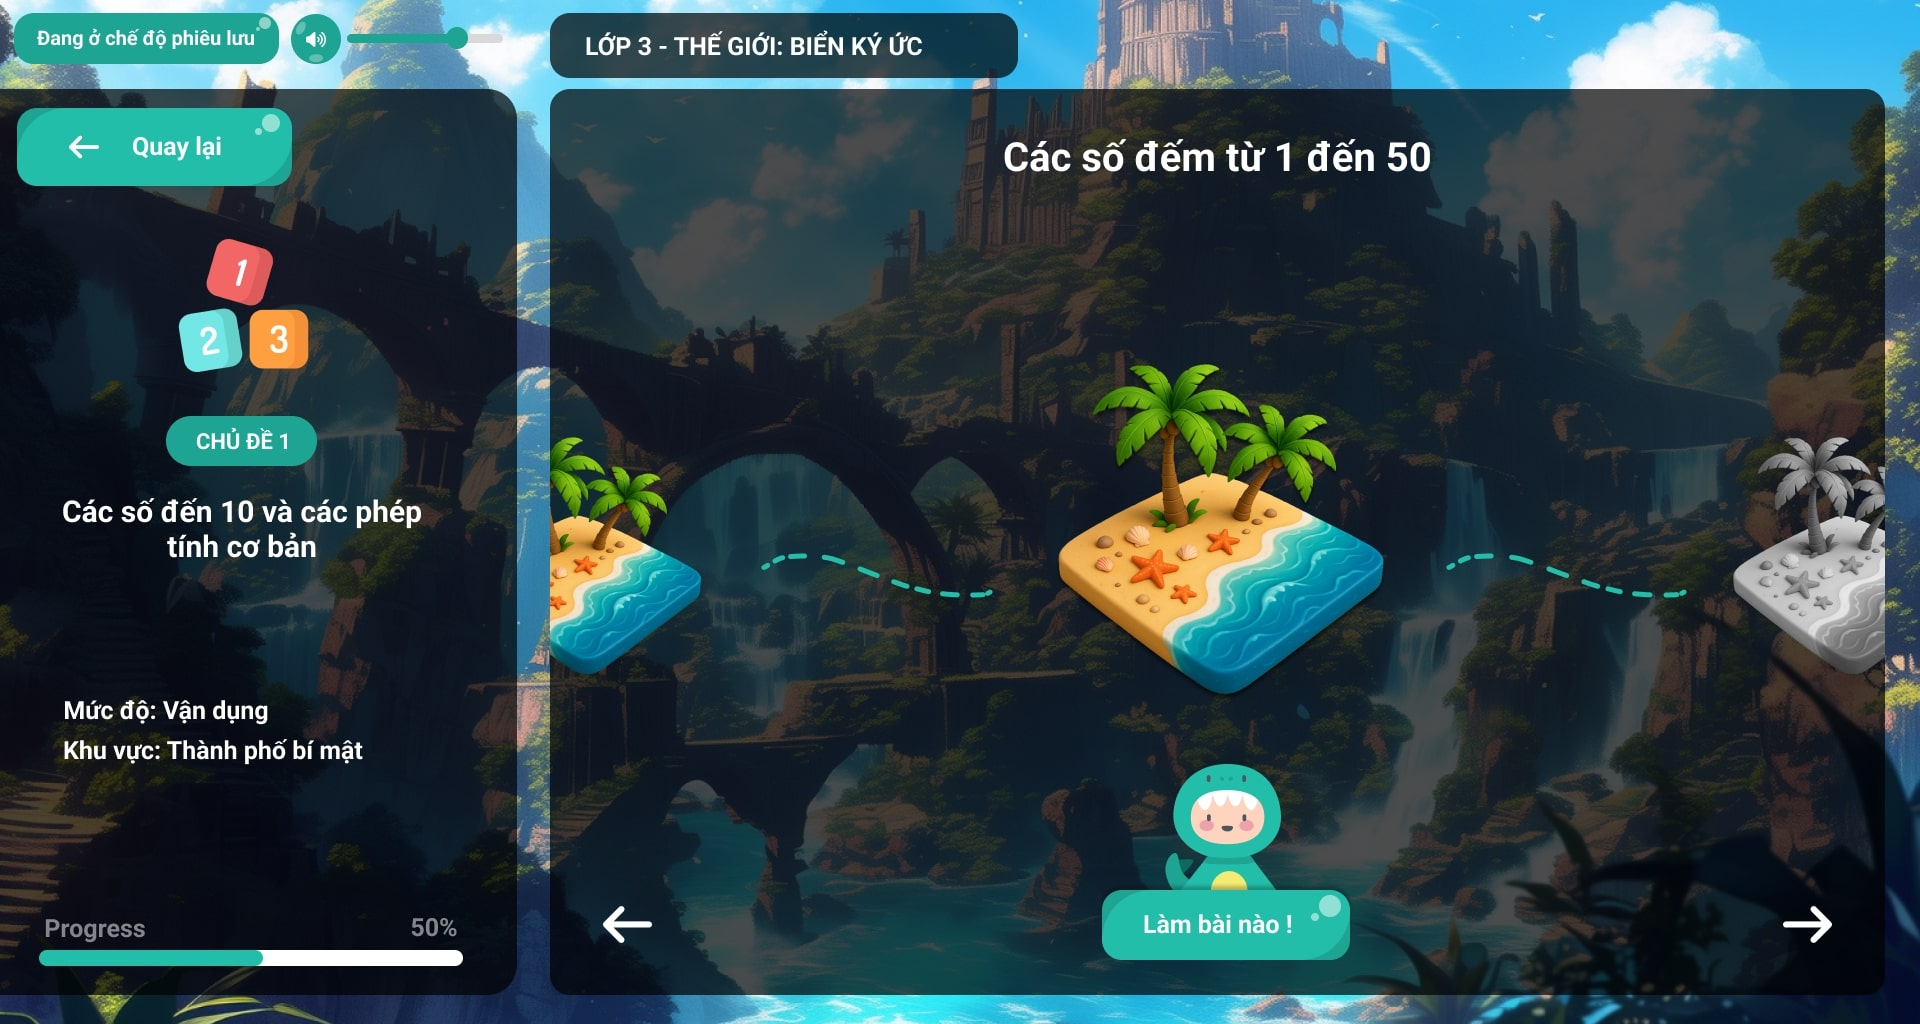
\includegraphics[width=\textwidth]{Image/UI/Milestones/Paths-G3-VD.jpg}
			\vspace{0.2cm}
			\caption{Lớp 3 - Vận dụng}
			\label{fig:h3}
		\end{minipage}
		\hspace{0.1cm}
		\begin{minipage}{0.45\textwidth}
			\centering
			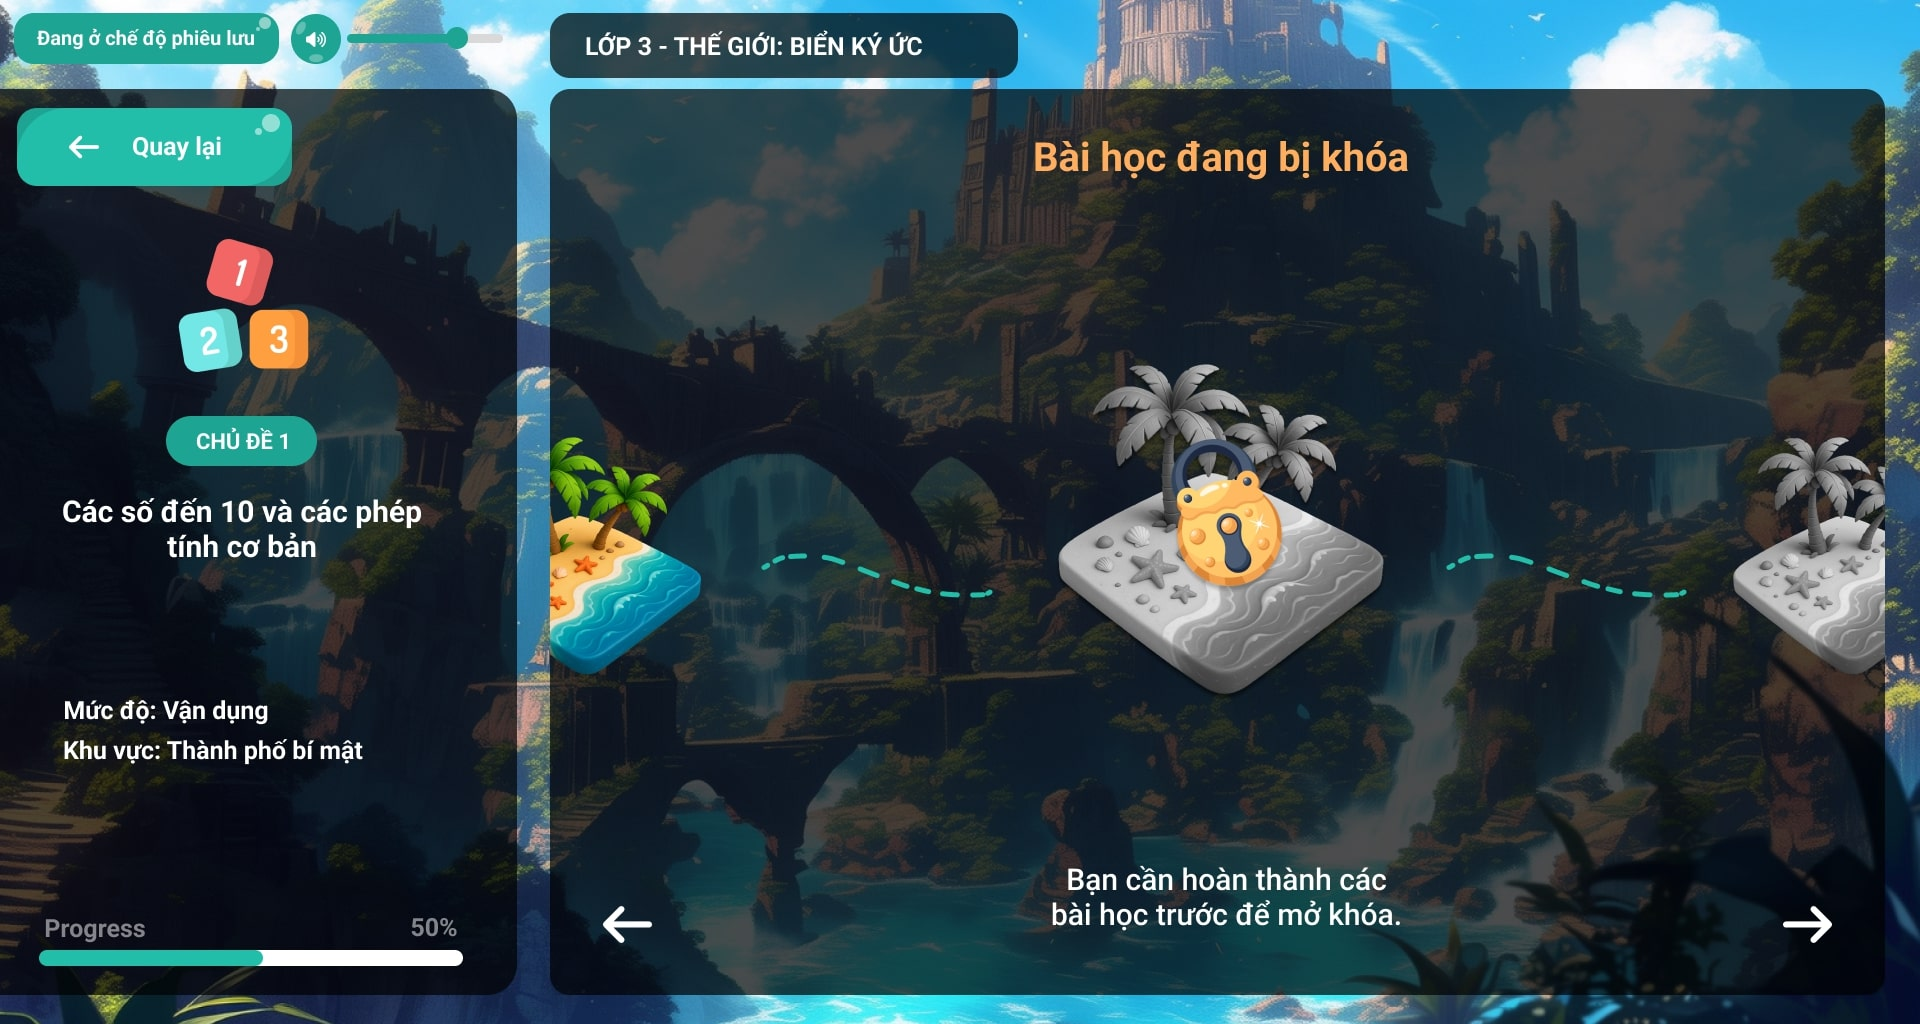
\includegraphics[width=\textwidth]{Image/UI/Milestones/Paths-G3-Locked.jpg}
			\vspace{0.2cm}
			\caption{Lớp 3 - Milestone bị khóa}
			\label{fig:l3}
		\end{minipage}
	\end{figure}
	
	\vspace{0.4cm}
	
	% --- Trang Chủ đề của Lớp 4 ---
	\noindent Thế giới của Lớp 4 được thiết kế với bối cảnh sa mạc. Các hình từ \ref{fig:e4} đến \ref{fig:h4} là thiết kế cho trang chủ đề của lớp 4 ứng với các mức độ khó khác nhau của bài học. Giao diện khóa của các bài học (milestone) được thiết kế như \textit{Hình \ref{fig:l4}}.
	\begin{figure}[H]
		\centering
		\begin{minipage}{0.45\textwidth}
			\centering
			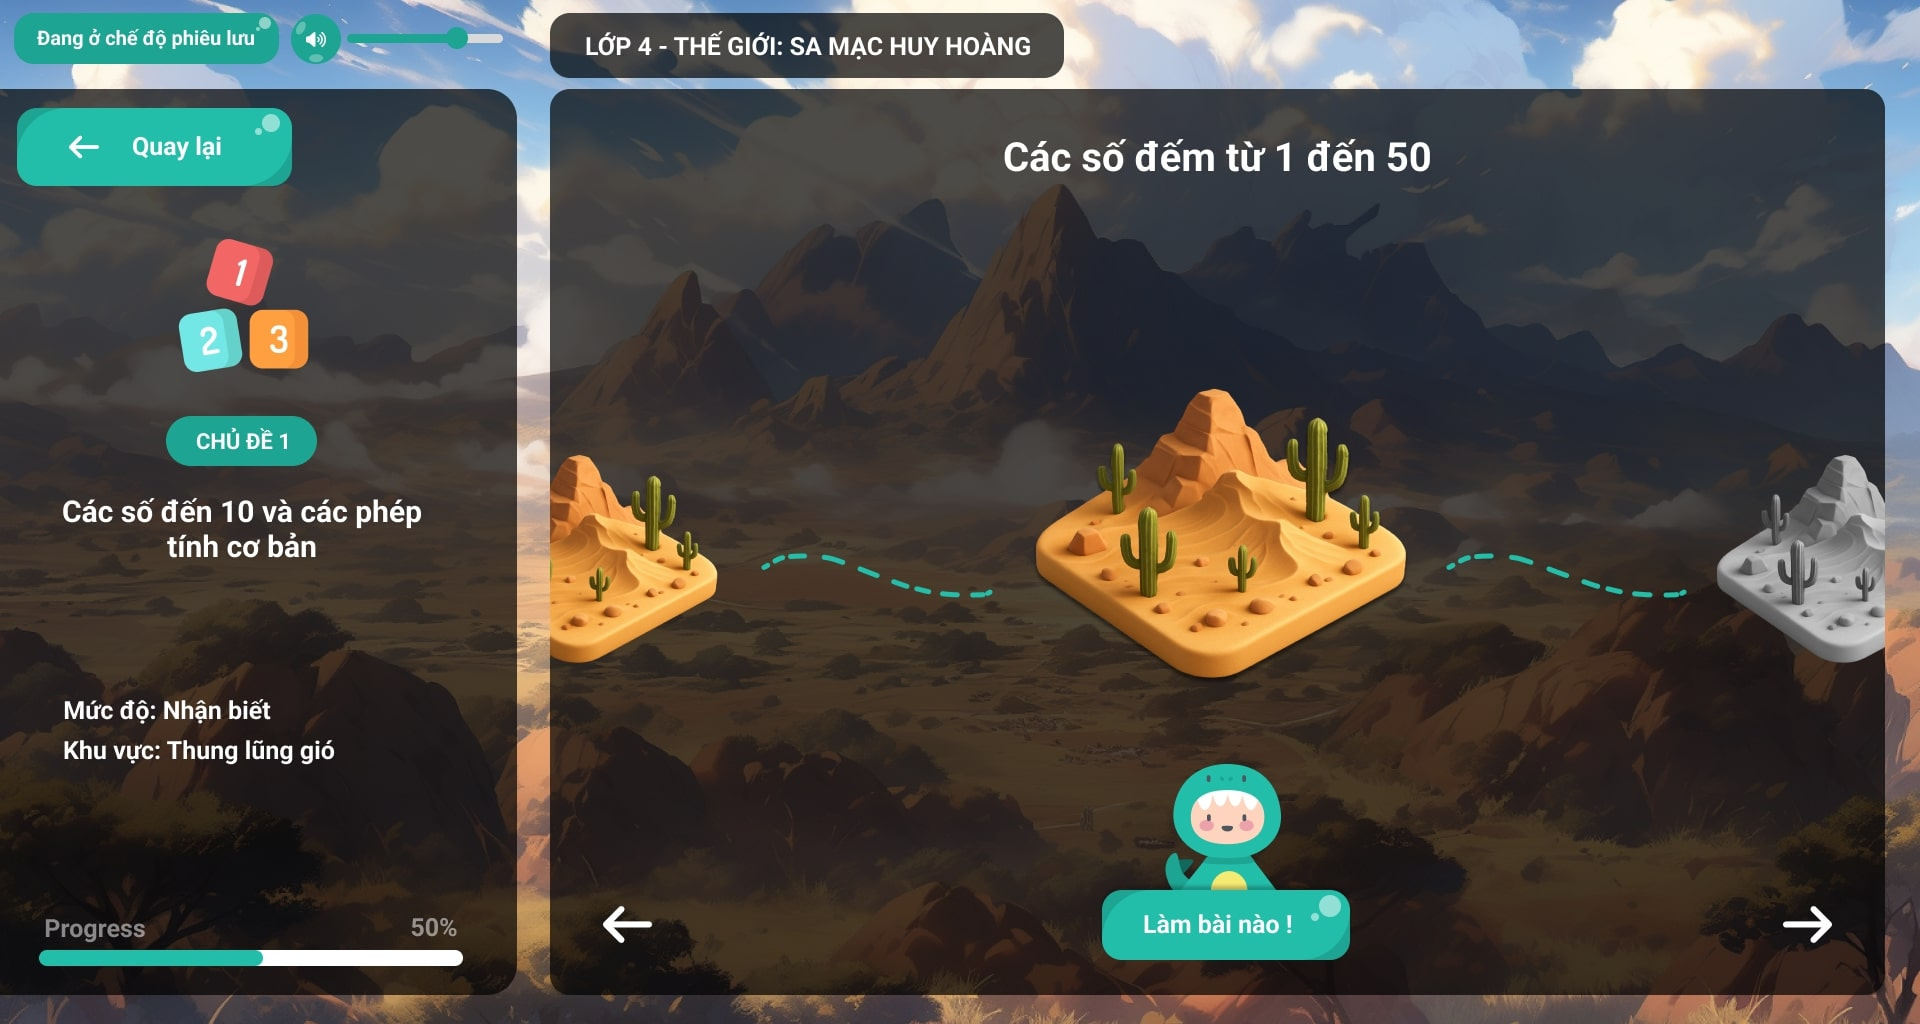
\includegraphics[width=\textwidth]{Image/UI/Milestones/Paths-G4-NB.jpg}
			\vspace{0.2cm}
			\caption{Lớp 4 - Nhận biết}
			\label{fig:e4}
		\end{minipage}
		\hspace{0.1cm}
		\begin{minipage}{0.45\textwidth}
			\centering
			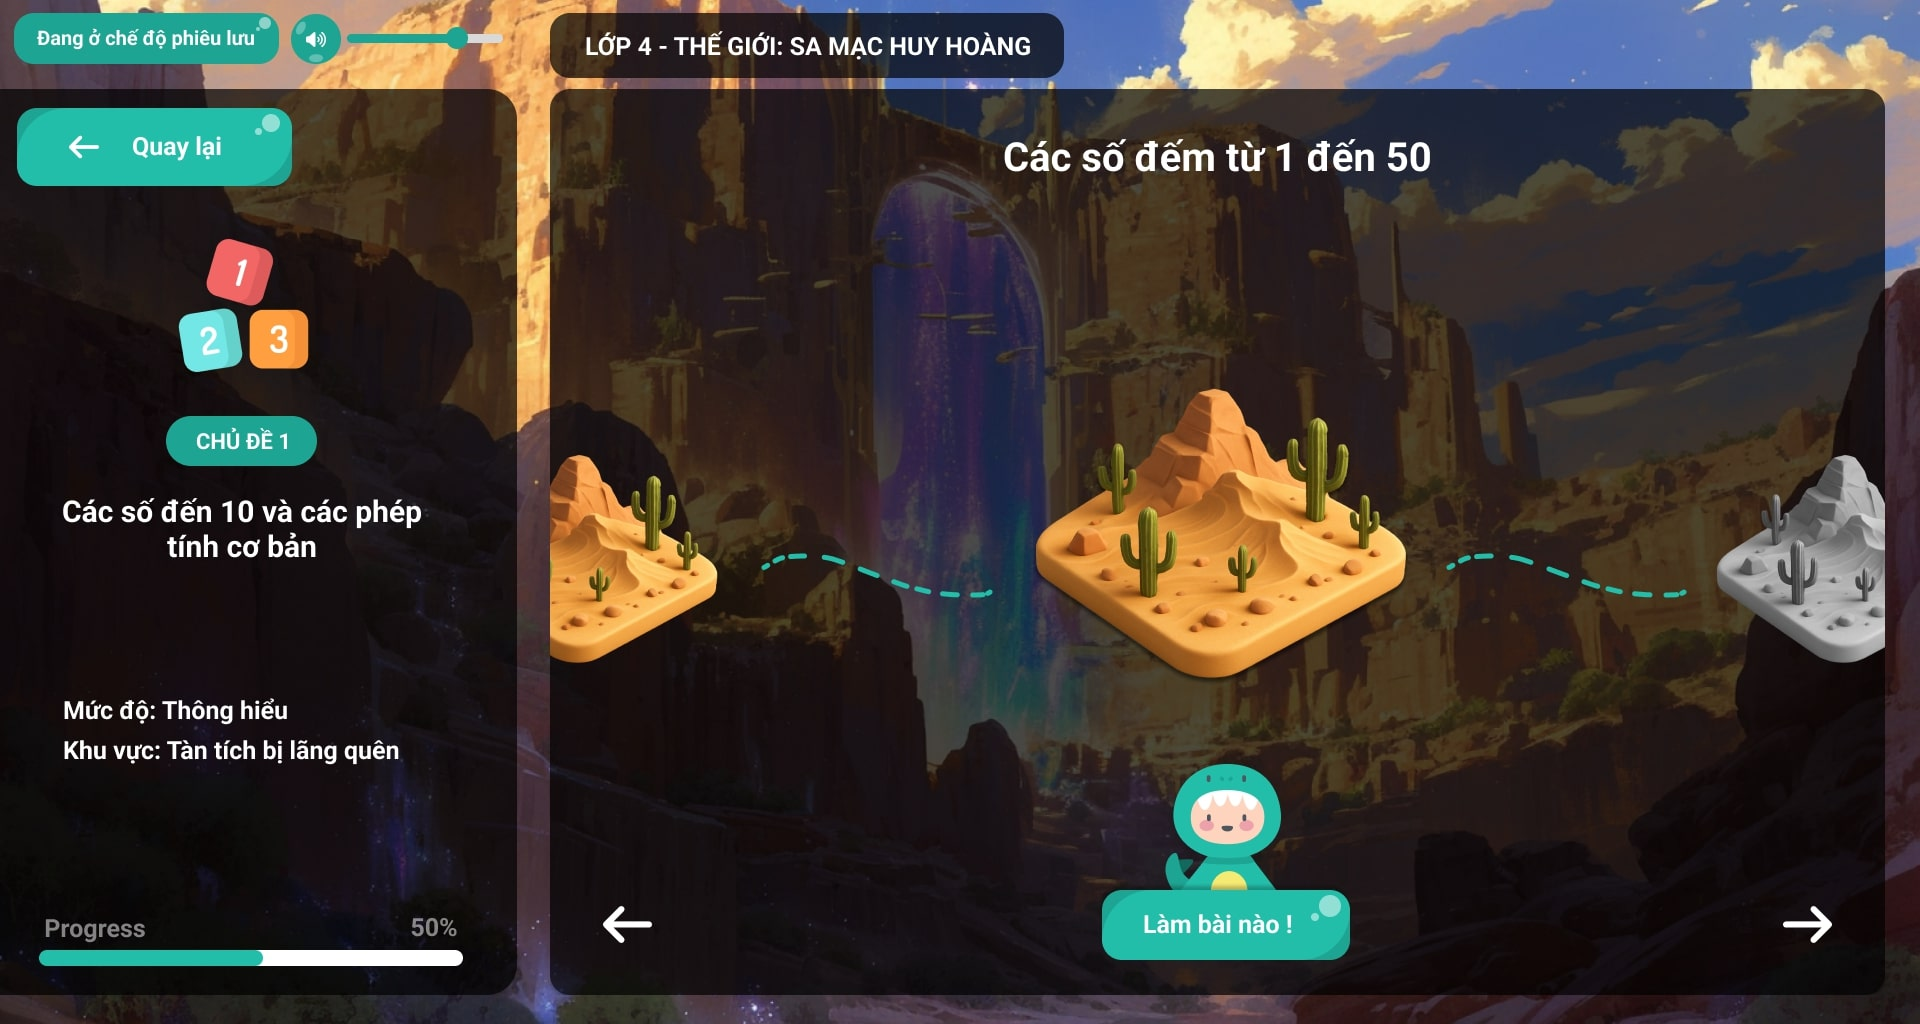
\includegraphics[width=\textwidth]{Image/UI/Milestones/Paths-G4-TH.jpg}
			\vspace{0.2cm}
			\caption{Lớp 4 - Thông hiểu}
		\end{minipage}
		
		\vspace{0.4cm}
		
		\begin{minipage}{0.45\textwidth}
			\centering
			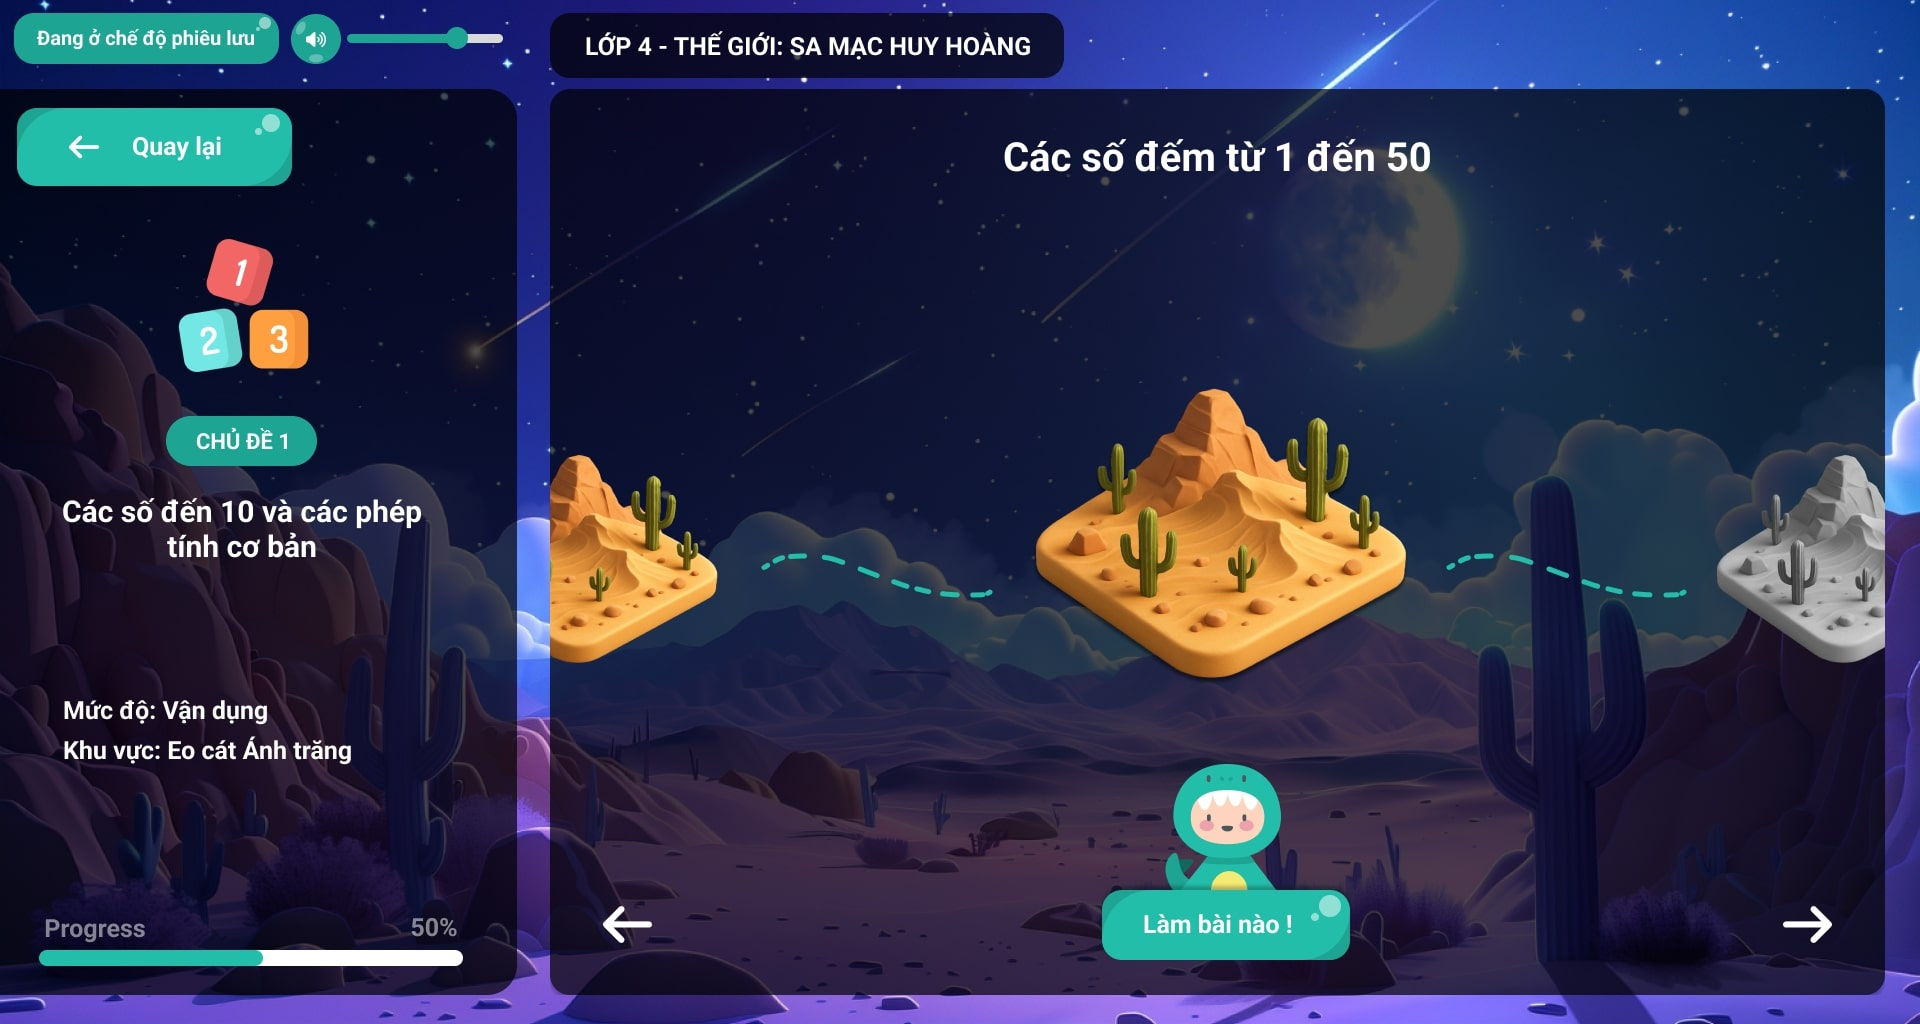
\includegraphics[width=\textwidth]{Image/UI/Milestones/Paths-G4-VD.jpg}
			\vspace{0.2cm}
			\caption{Lớp 4 - Vận dụng}
			\label{fig:h4}
		\end{minipage}
		\hspace{0.1cm}
		\begin{minipage}{0.45\textwidth}
			\centering
			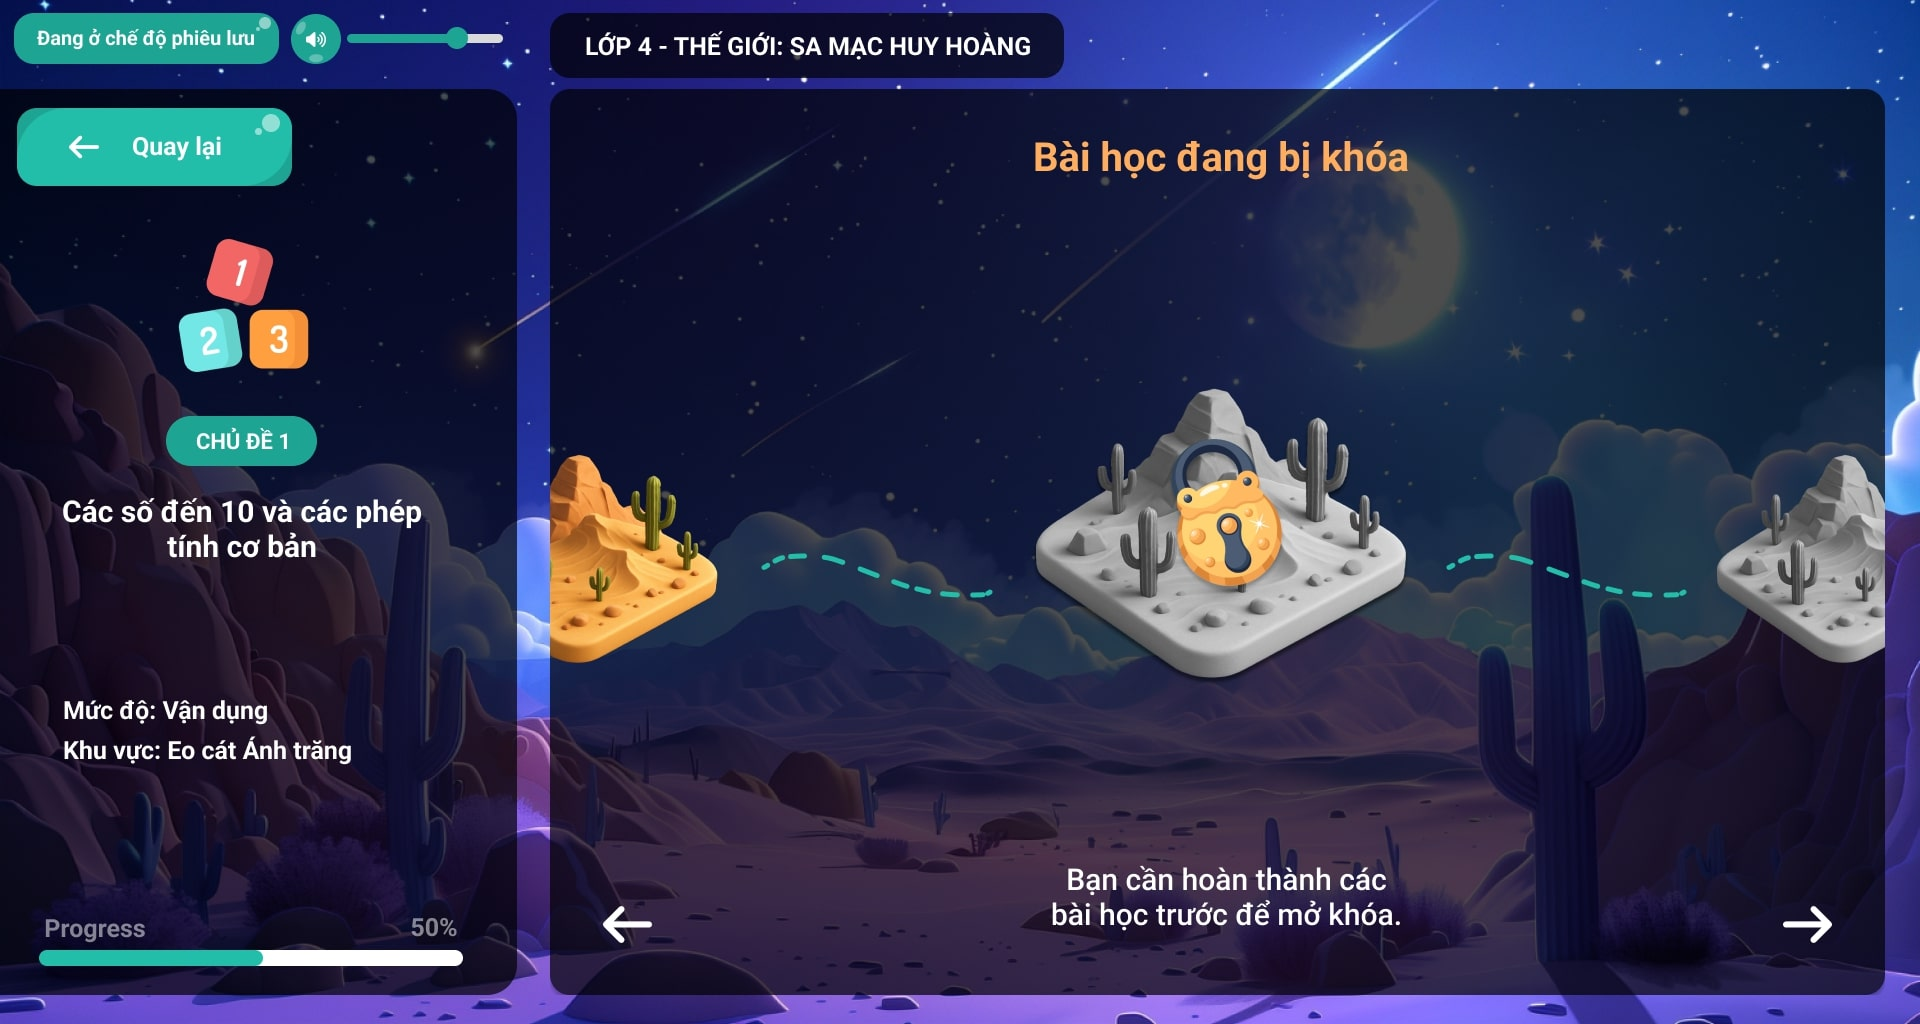
\includegraphics[width=\textwidth]{Image/UI/Milestones/Paths-G4-Locked.jpg}
			\vspace{0.2cm}
			\caption{Lớp 4 - Milestone bị khóa}
			\label{fig:l4}
		\end{minipage}
	\end{figure}
	
	\vspace{0.4cm}
	
	% --- Trang Chủ đề của Lớp 5 ---
	\noindent Thế giới của Lớp 5 được thiết kế với bối cảnh núi lửa. Các hình từ \ref{fig:e5} đến \ref{fig:h5} là thiết kế cho trang chủ đề của lớp 5 ứng với các mức độ khó khác nhau của bài học. Giao diện khóa của các bài học (milestone) được thiết kế như \textit{Hình \ref{fig:l5}}.
	\begin{figure}[H]
		\centering
		\begin{minipage}{0.45\textwidth}
			\centering
			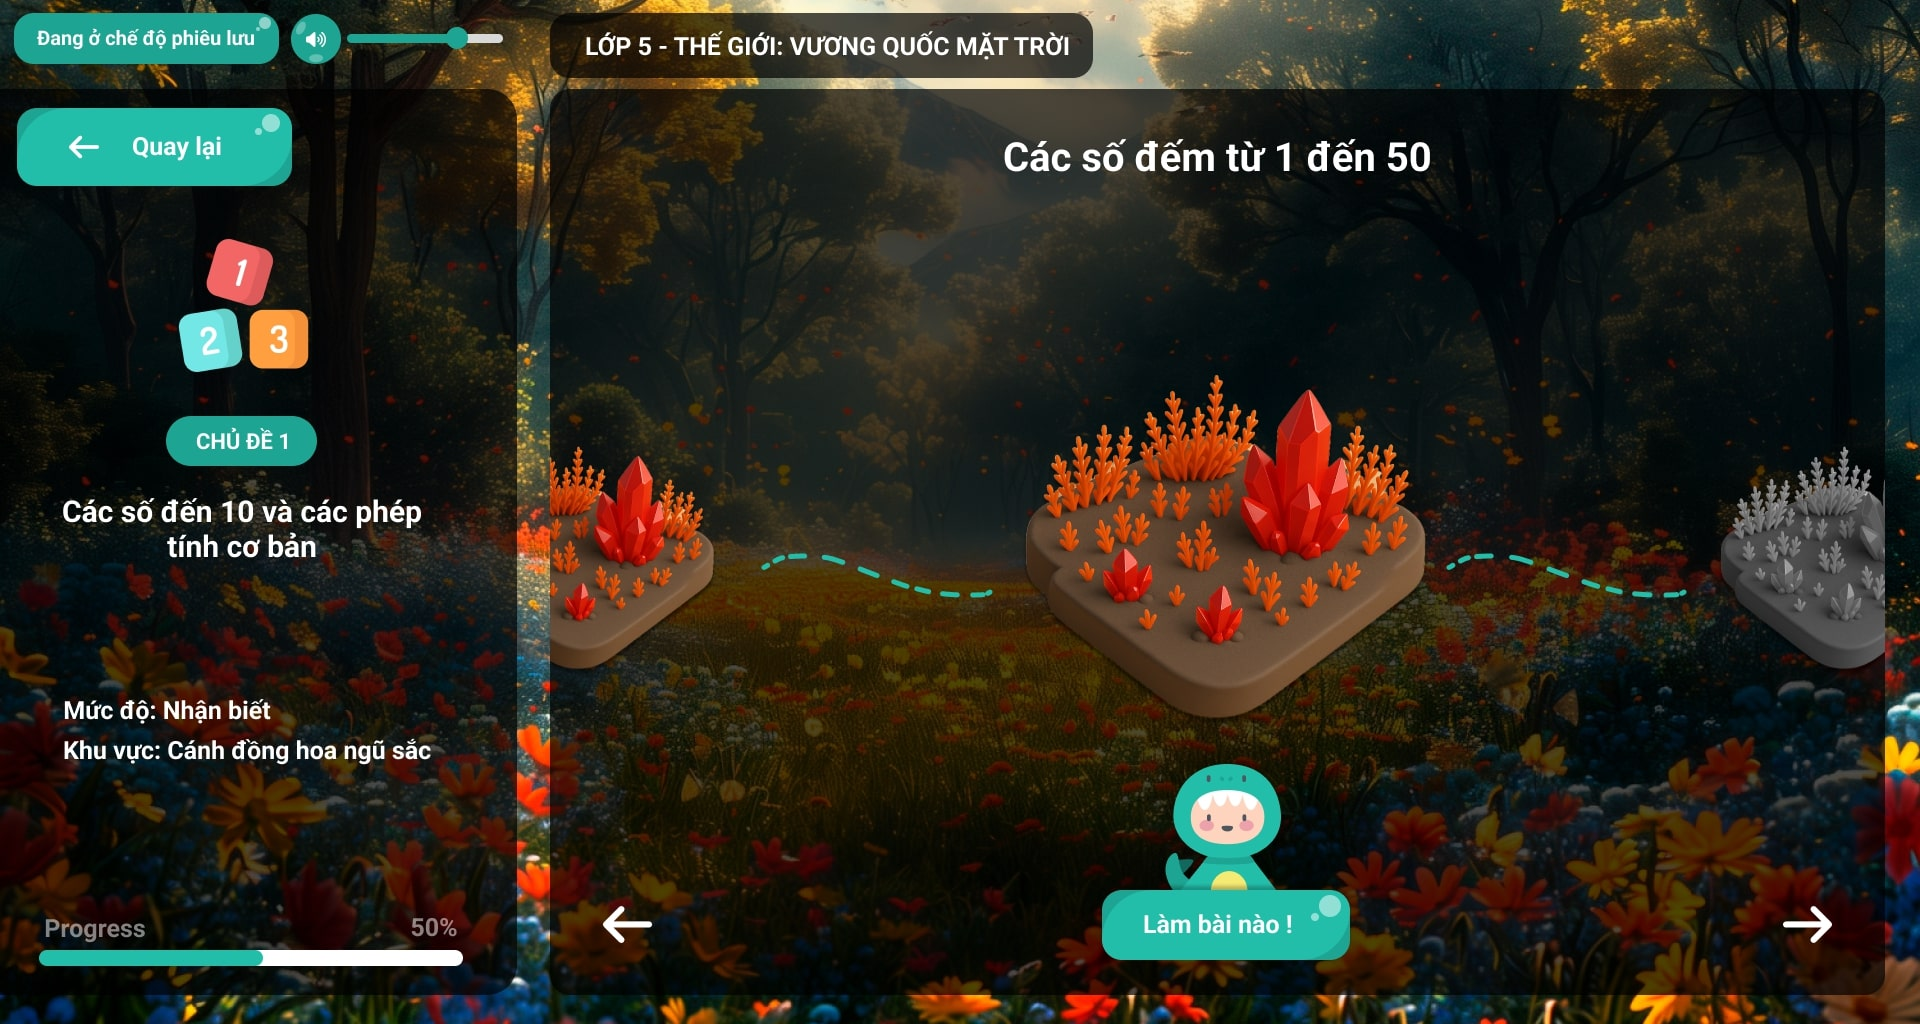
\includegraphics[width=\textwidth]{Image/UI/Milestones/Paths-G5-NB.jpg}
			\vspace{0.2cm}
			\caption{Lớp 5 - Nhận biết}
			\label{fig:e5}
		\end{minipage}
		\hspace{0.1cm}
		\begin{minipage}{0.45\textwidth}
			\centering
			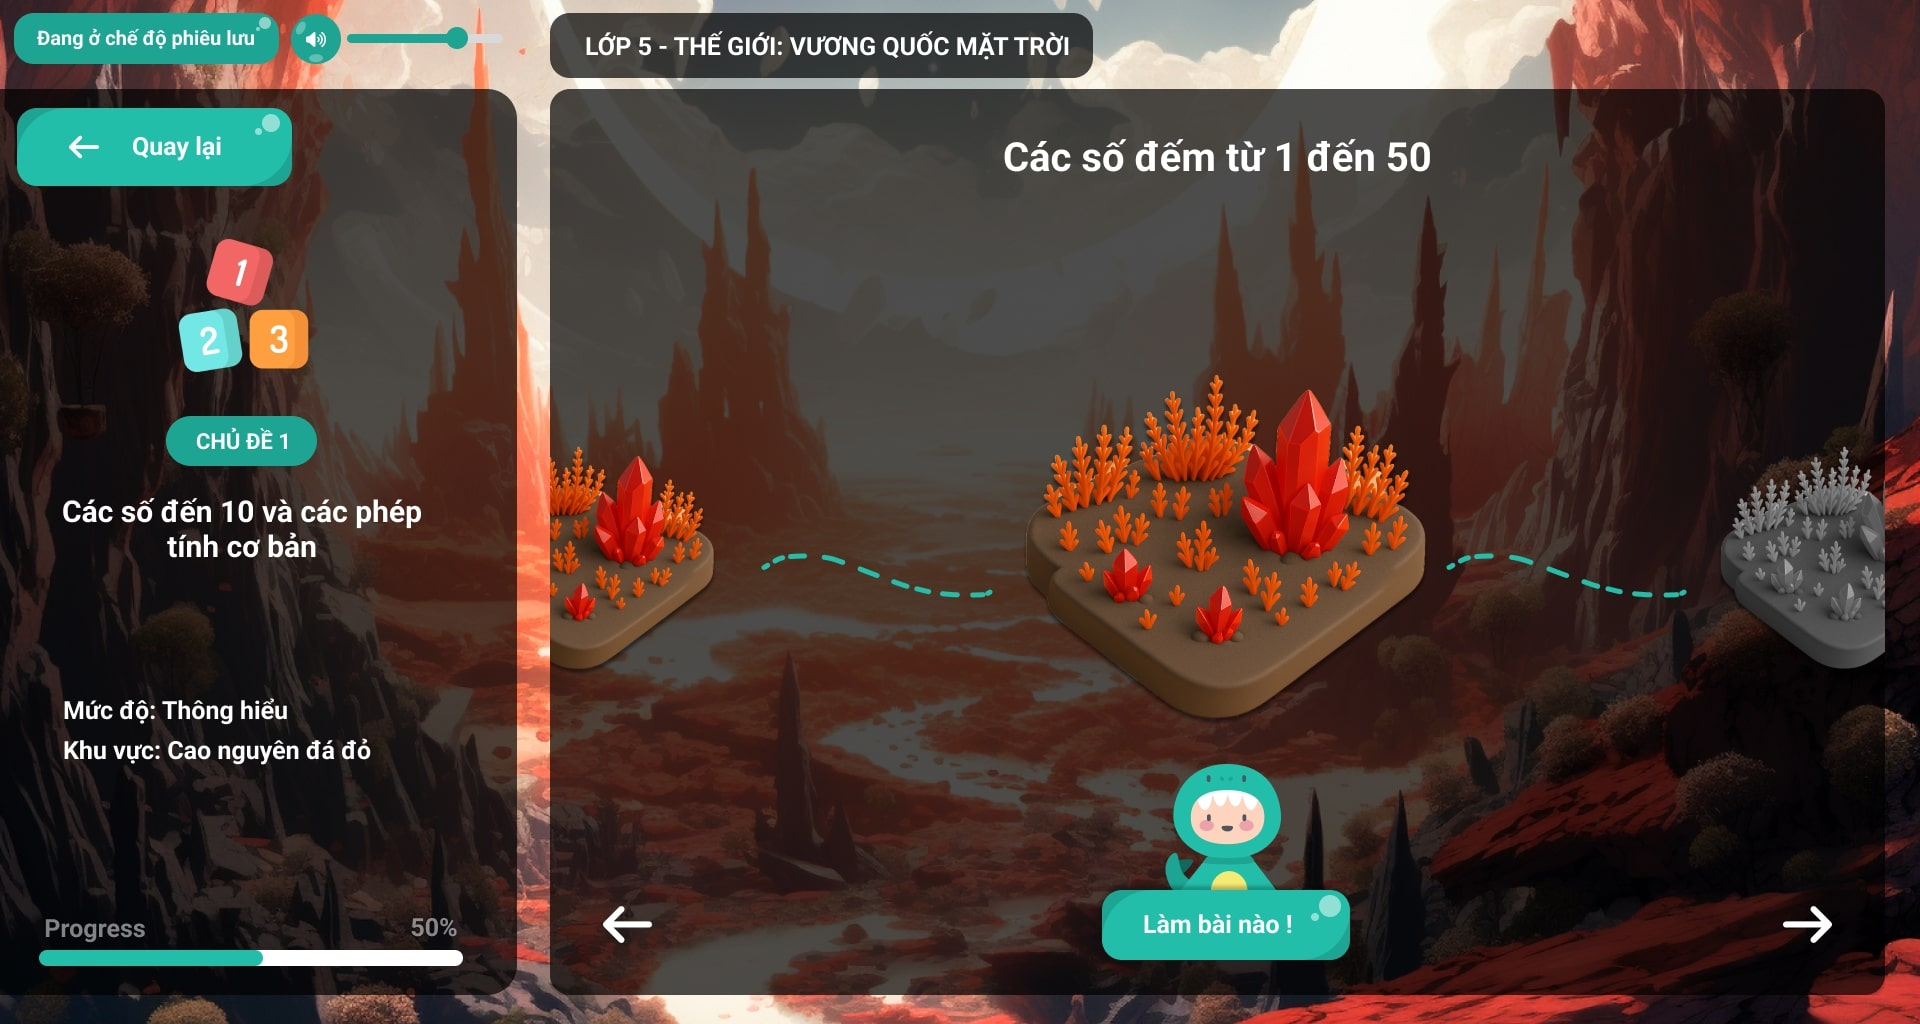
\includegraphics[width=\textwidth]{Image/UI/Milestones/Paths-G5-TH.jpg}
			\vspace{0.2cm}
			\caption{Lớp 5 - Thông hiểu}
		\end{minipage}
		
		\vspace{0.4cm}
		
		\begin{minipage}{0.45\textwidth}
			\centering
			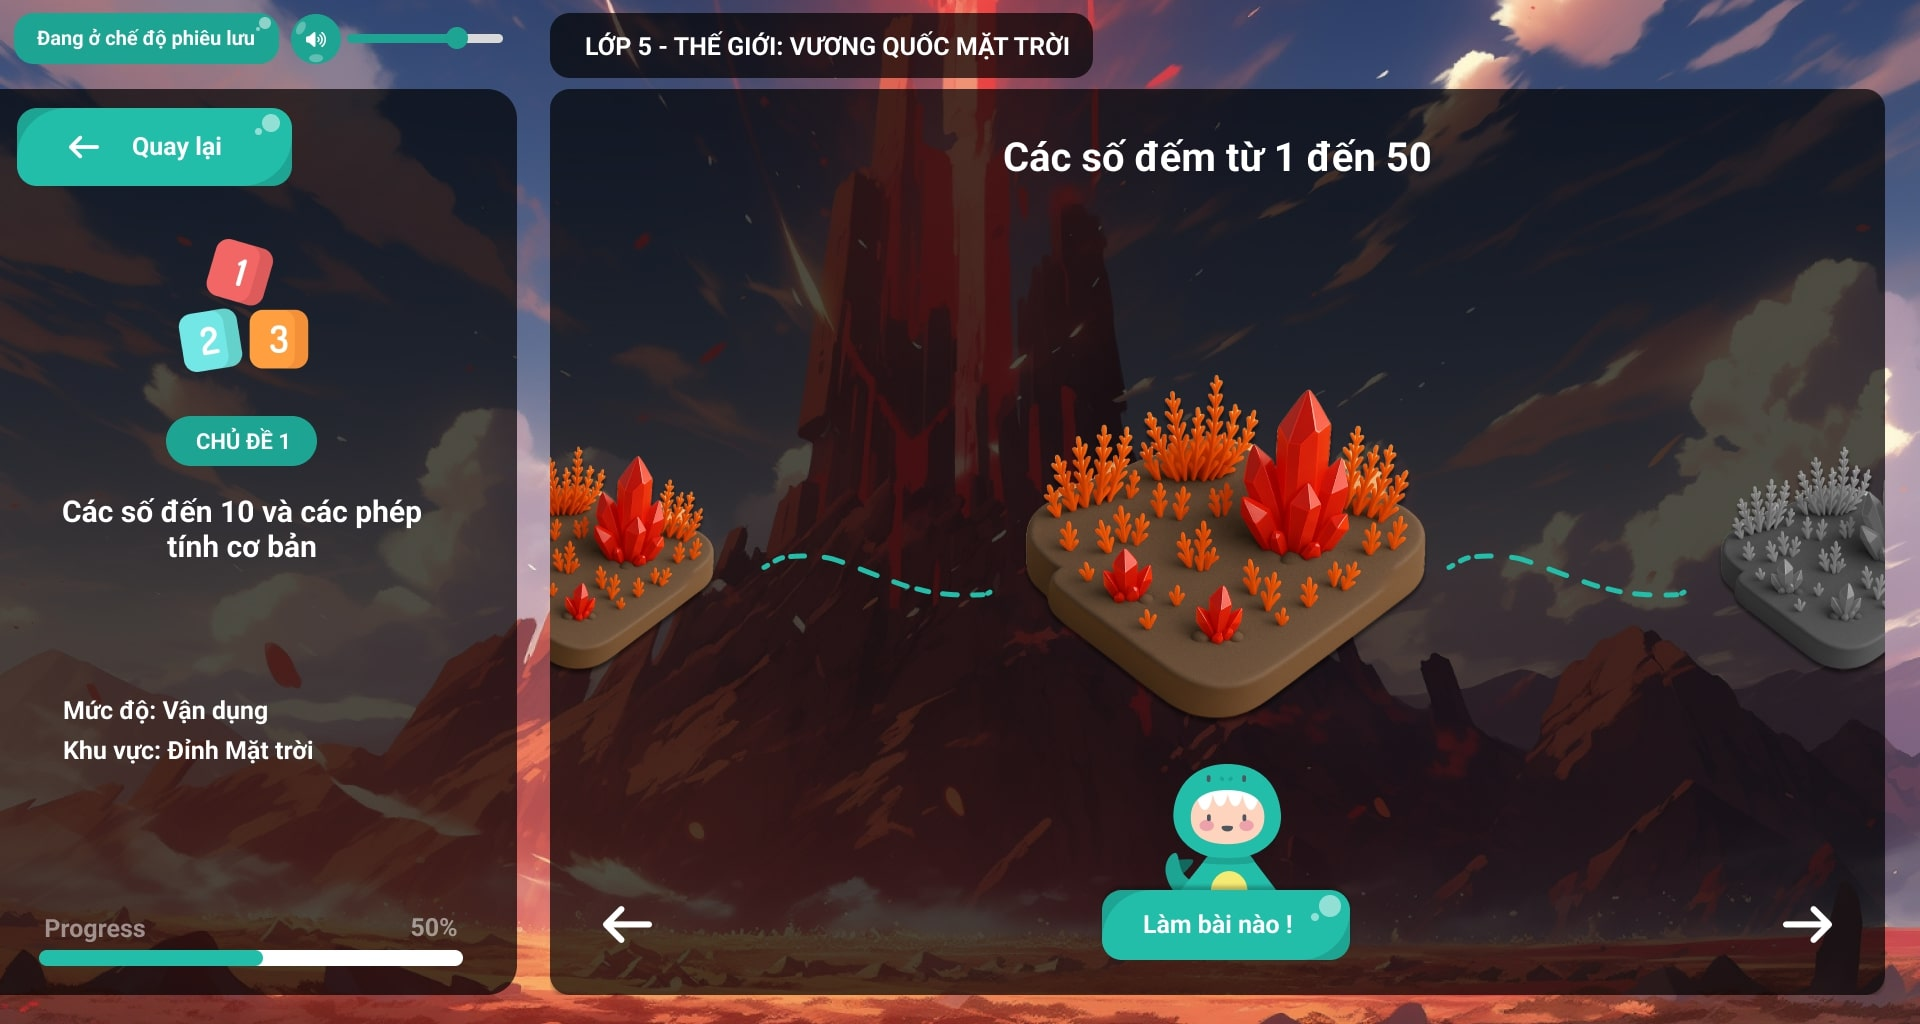
\includegraphics[width=\textwidth]{Image/UI/Milestones/Paths-G5-VD.jpg}
			\vspace{0.2cm}
			\caption{Lớp 5 - Vận dụng}
			\label{fig:h5}
		\end{minipage}
		\hspace{0.1cm}
		\begin{minipage}{0.45\textwidth}
			\centering
			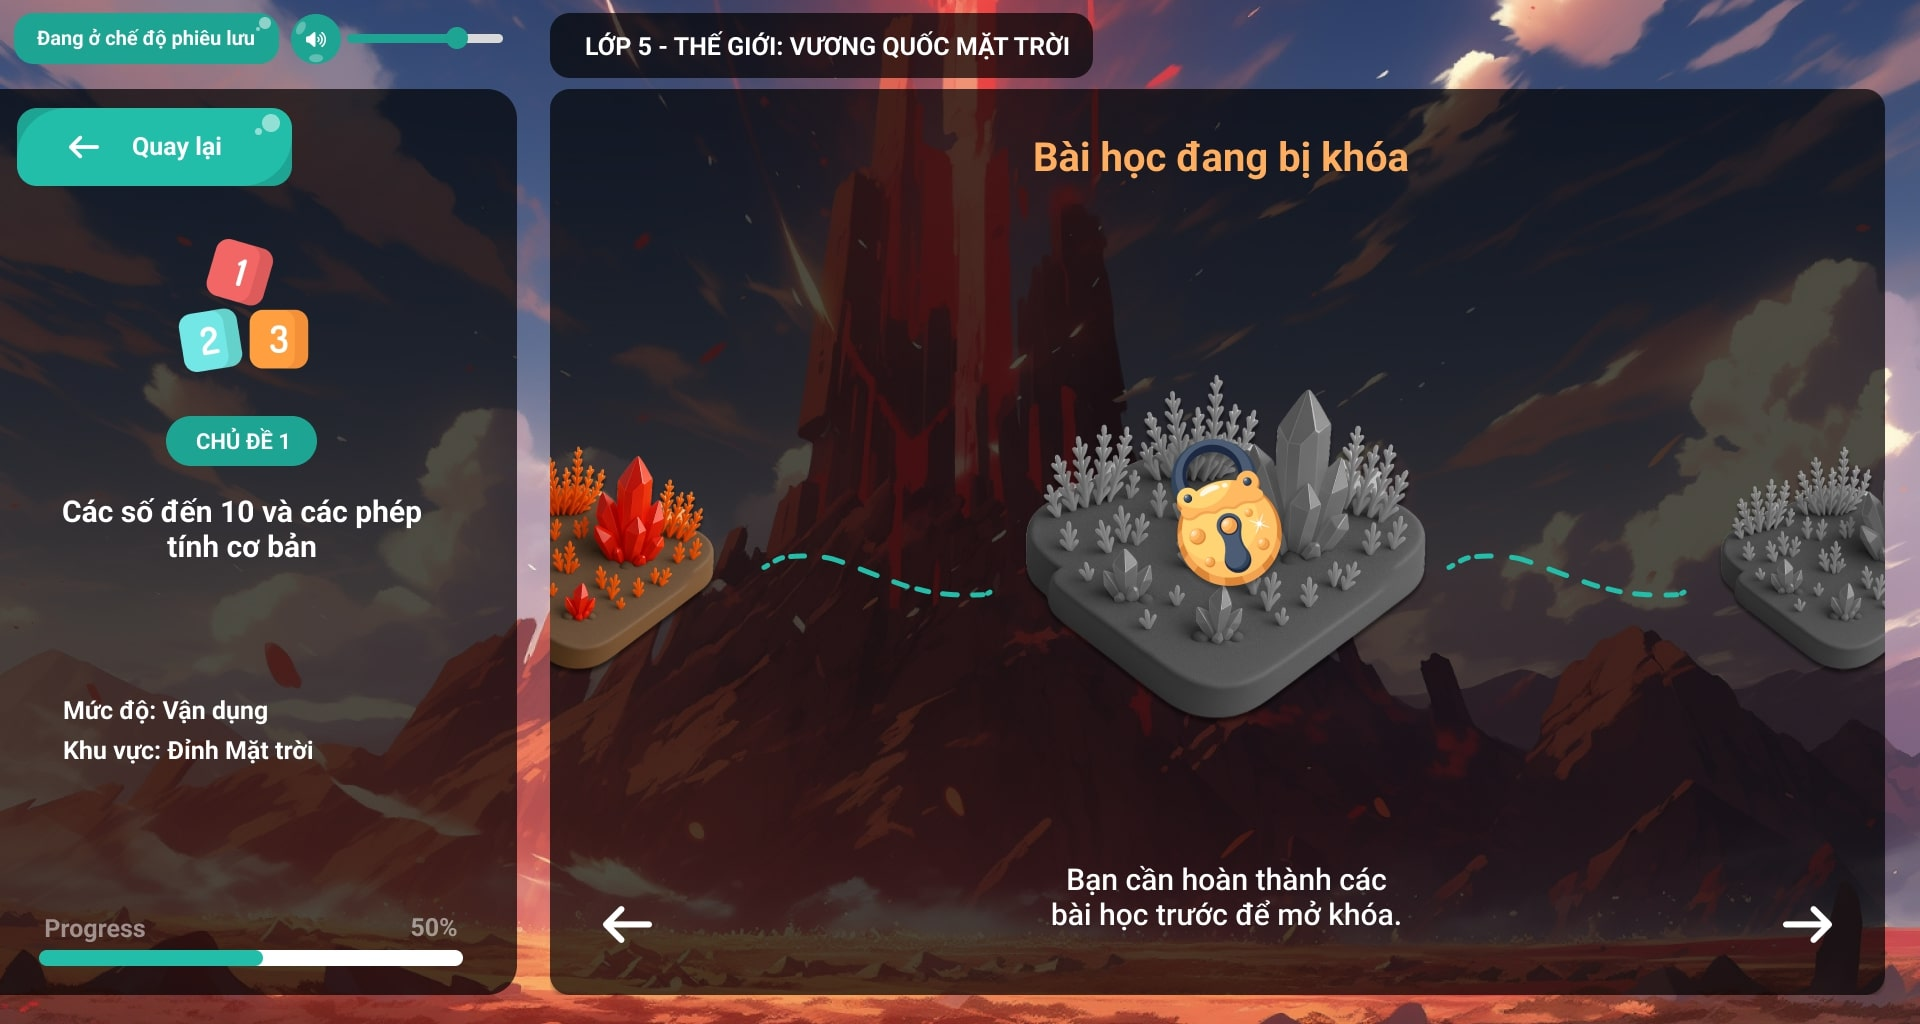
\includegraphics[width=\textwidth]{Image/UI/Milestones/Paths-G5-Locked.jpg}
			\vspace{0.2cm}
			\caption{Lớp 5 - Milestone bị khóa}
			\label{fig:l5}
		\end{minipage}
	\end{figure}

\subsubsection{Trang Bài tập}
\label{subsubsec:exercise}
\textbf{Trang Bài tập} chỉ có thể được truy cập bằng cách bấm vào nút \textit{Làm bài} ở \textbf{Trang Chủ đề} được mô tả ở mục \ref{subsubsec:topic}. Tại trang này người dùng có thể làm các dạng bài tập tương tác như kéo thả, trắc nghiệm, đúng/sai, điền khuyết, lắp ghép (xem chi tiết ở mục \ref{subsec:interact}). Phần tên bài học và danh sách các câu hỏi được hiển thị trên sidebar nằm bên trái giao diện. Người dùng có thể chuyển câu hỏi bằng cách nhấn vào các nút được đánh số thứ tự tương ứng. Người dùng có thể nộp bài bằng cách bấm vào nút \textit{Nộp bài} ở dưới cùng của sidebar. Với mỗi câu làm đúng, người dùng sẽ nhận được một lượng thạch anh nhất định. Giao diện làm bài tập hỗ trợ nhiều dạng tương tác khác nhau (xem chi tiết tại mục \ref{subsec:interact}).

\newline
Sau khi tương tác với bài tập, người dùng có thể bấm \textit{Kiểm tra đáp án} để kiểm tra câu trả lời của mình. Nếu trả lời đúng, giao diện sẽ giống như \textit{Hình \ref{fig:correct}}; nếu sai, giao diện sẽ giống như \textit{Hình \ref{fig:wrong}}.
\begin{figure}[H]
	\centering
	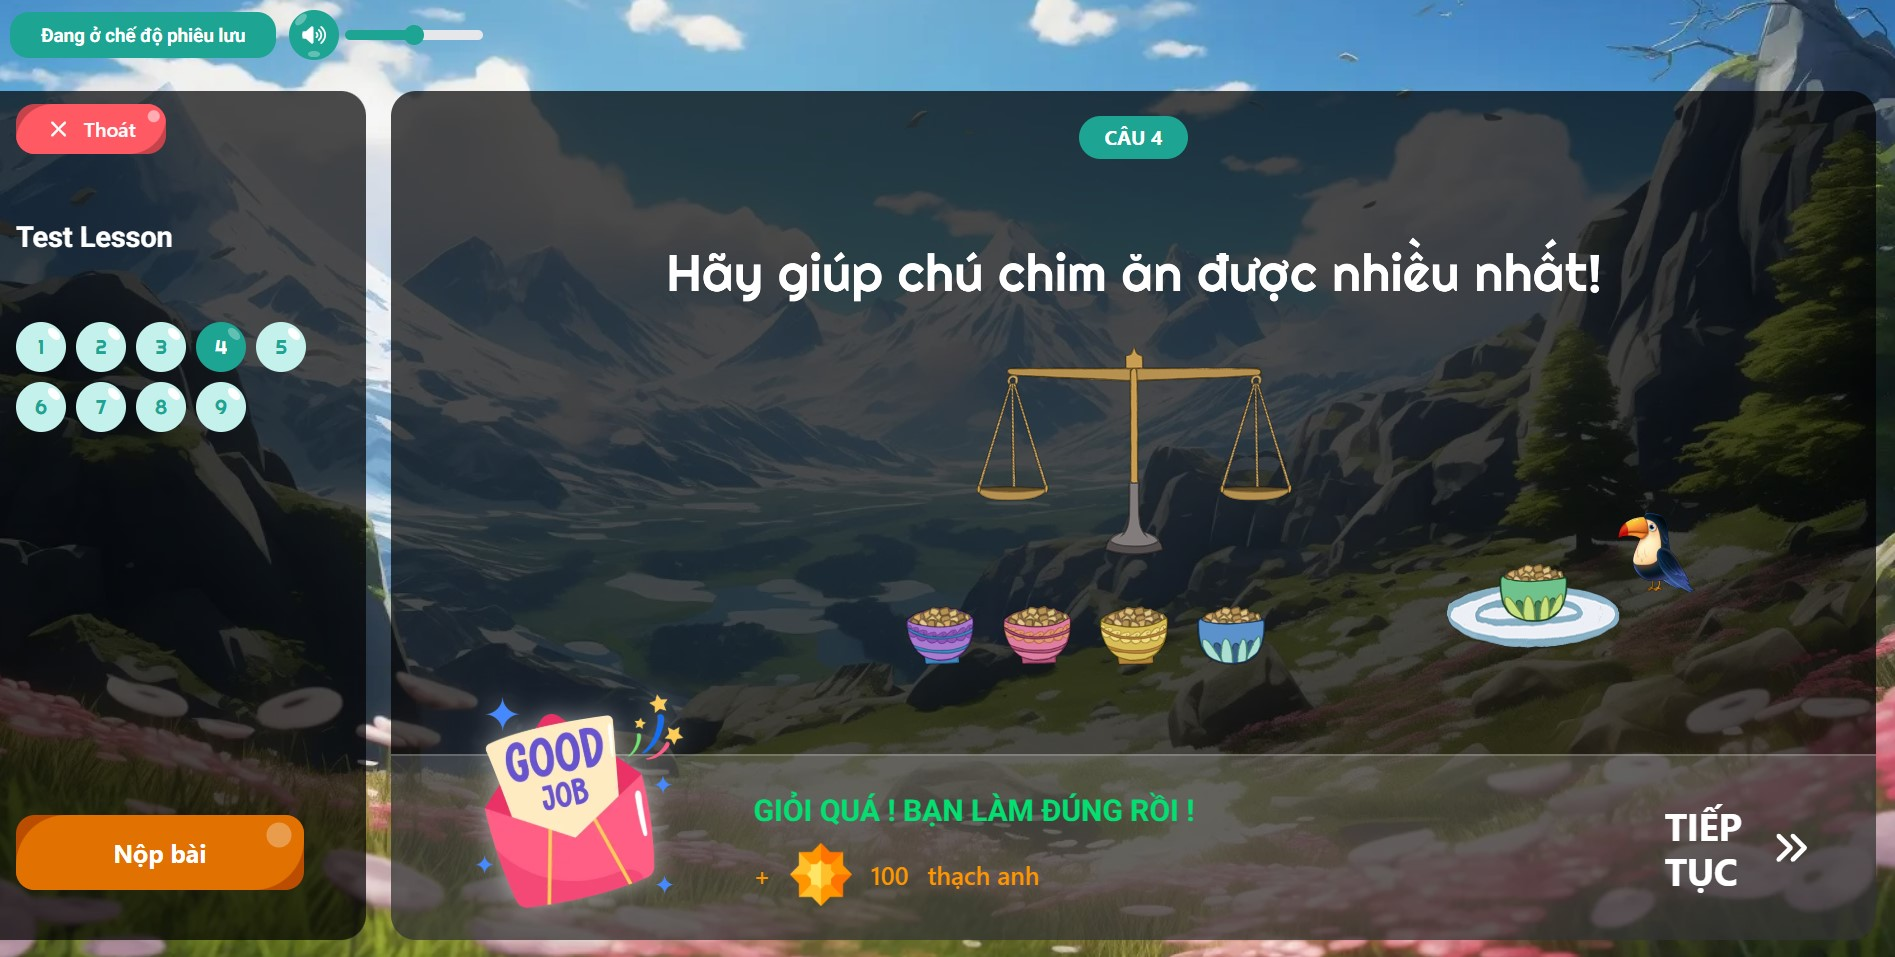
\includegraphics[width=0.9\textwidth]{Image/UI/Exercises/Correct.jpg}
	\vspace{0.6cm}
	\caption{Hiệu ứng chúc mừng khi làm đúng}
	\label{fig:correct}
\end{figure}
\begin{figure}[H]
	\centering
	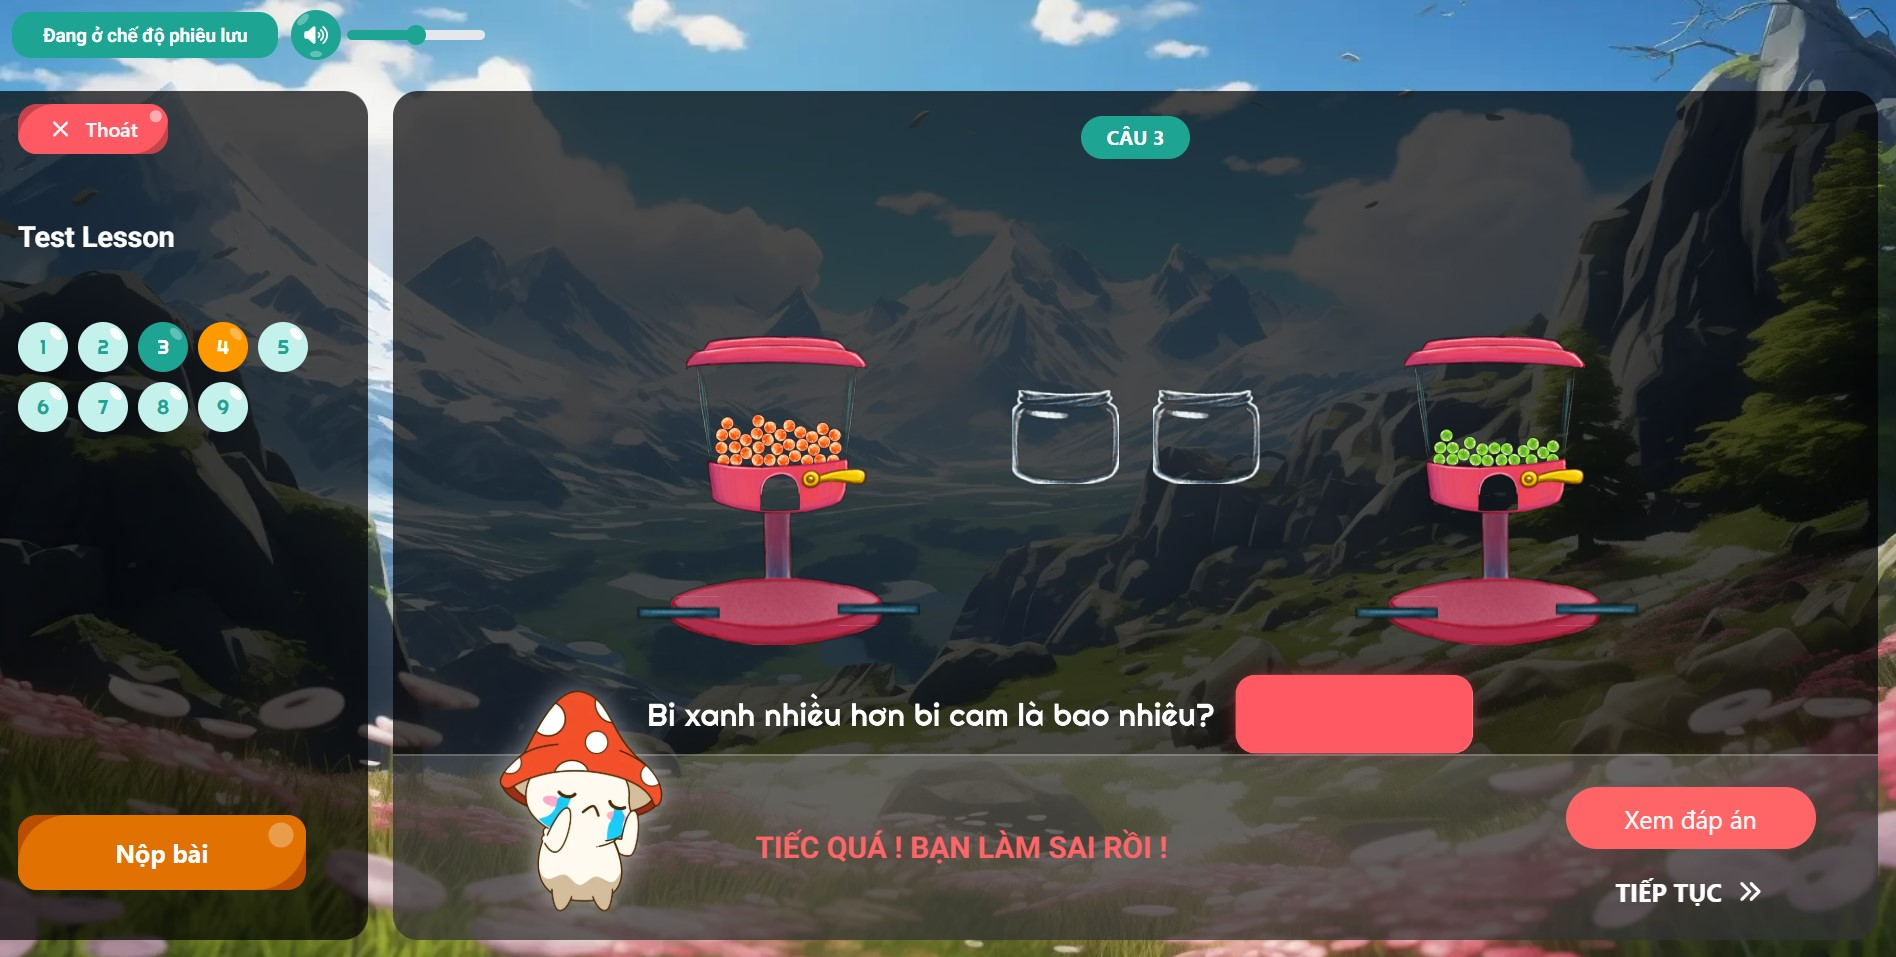
\includegraphics[width=\textwidth]{Image/UI/Exercises/Wrong.jpg}
	\vspace{0.6cm}
	\caption{Hiệu ứng chúc mừng khi làm đúng}
	\label{fig:wrong}
\end{figure}
\begin{figure}[H]
	\centering
	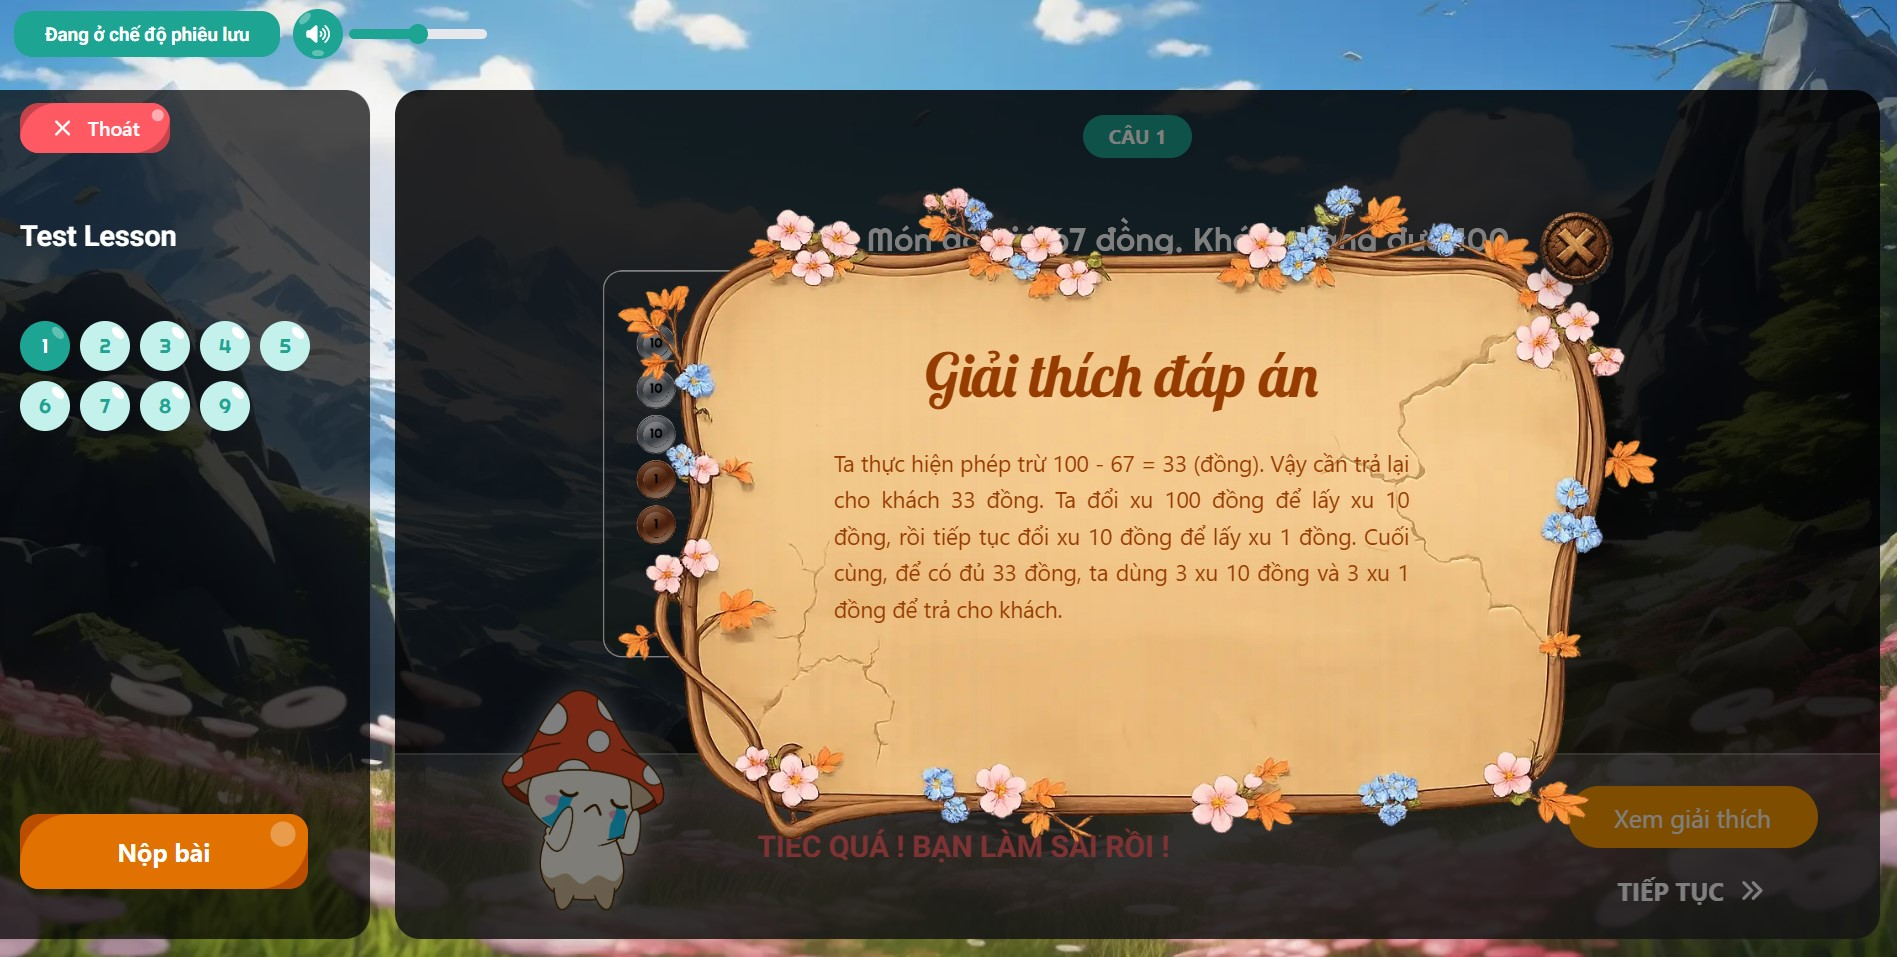
\includegraphics[width=\textwidth]{Image/UI/Exercises/Explain.jpg}
	\vspace{0.6cm}
	\caption{Xem giải thích đáp án khi làm sai}
	\label{fig:explain}
\end{figure}

Sau khi người dùng hoàn thành tất cả câu hỏi, giao diện kết quả sẽ được hiển thị như giao diện sẽ giống như \textit{Hình \ref{fig:result}} bao gồm tên lớp, chủ đề, tên bài học, tổng số điểm đạt được và tổng số thạch anh nhận được.
\begin{figure}[H]
	\centering
	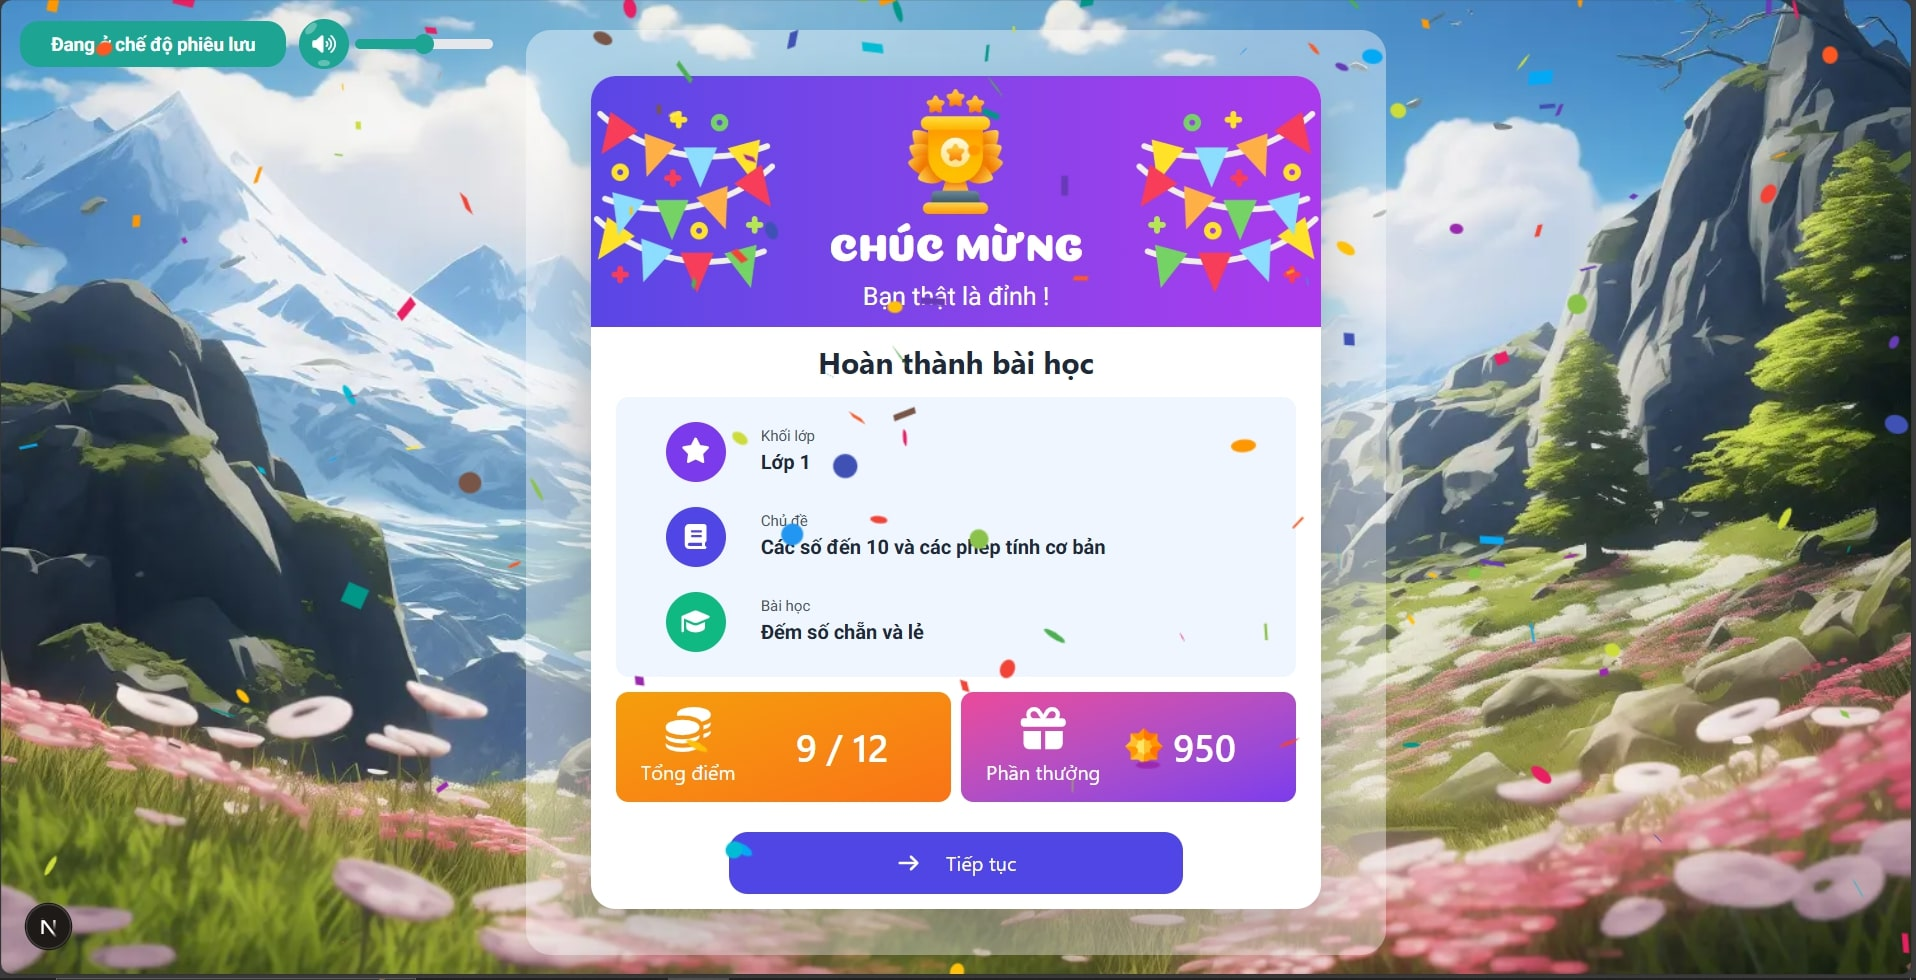
\includegraphics[width=0.9\textwidth]{Image/UI/Exercises/Finish.jpg}
	\vspace{0.6cm}
	\caption{Giao diện kết quả sau khi hoàn thành bài học}
	\label{fig:result}
\end{figure}

\subsubsection{Trang Đấu trường}
\label{subsubsec:arena}
Người dùng có thể tham gia làm bài thi đấu trường theo tuần, xem thời gian còn lại của đấu trường, xem bậc xếp hạng hiện tại của mình, xem bảng xếp hạng tuần và xem thể lệ đấu trường. Để bắt đầu làm bài thi, người dùng chỉ cần bấm nút \textit{Tham gia ngay} bên trong khung màu cam được hiển thị trên giao diện. Sau khi bấm nút, người dùng sẽ được điều hướng sang \textbf{Trang Bài thi} được mô tả ở mục \ref{subsubsec:exam}. Giao diện chính của trang đấu trường được thiết kế như \textit{Hình \ref{fig:arena}}.
\begin{figure}[H]
	\centering
	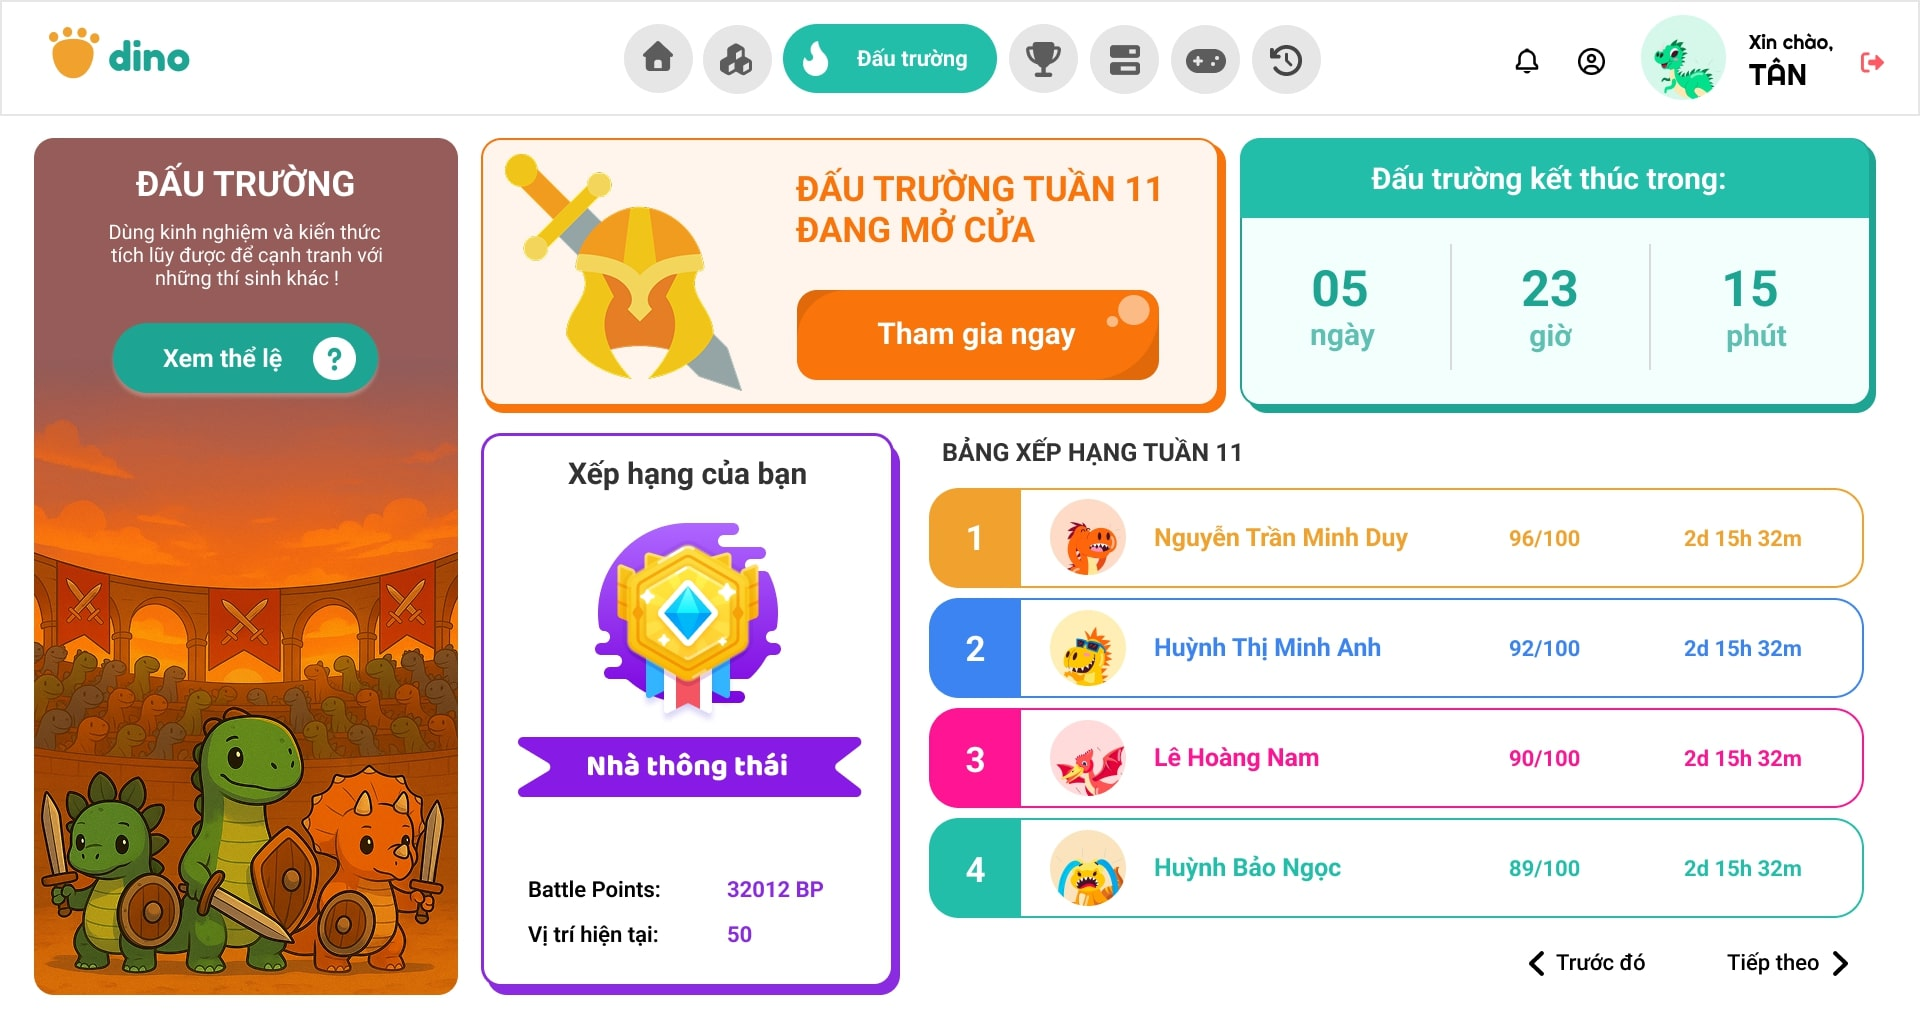
\includegraphics[width=0.9\textwidth]{Image/UI/Main-Student/Arena-Home.jpg}
	\vspace{0.6cm}
	\caption{Trang Đấu trường}
	\label{fig:arena}
\end{figure}

\vspace{0.2cm}
\newline
Để xem thể lệ cuộc thi, người dùng bấm vào nút \textit{Xem thể lệ} nằm ở bên trái của giao diện. Trang thể lệ đấu trường sẽ được phóng to, người dùng có thể bấm chuyển trang để đọc hết tất cả các thể lệ.
\begin{figure}[H]
	\centering
	\begin{minipage}{1.0\textwidth} % Sử dụng toàn bộ độ rộng văn bản
		\centering
		
		% Dòng 1
		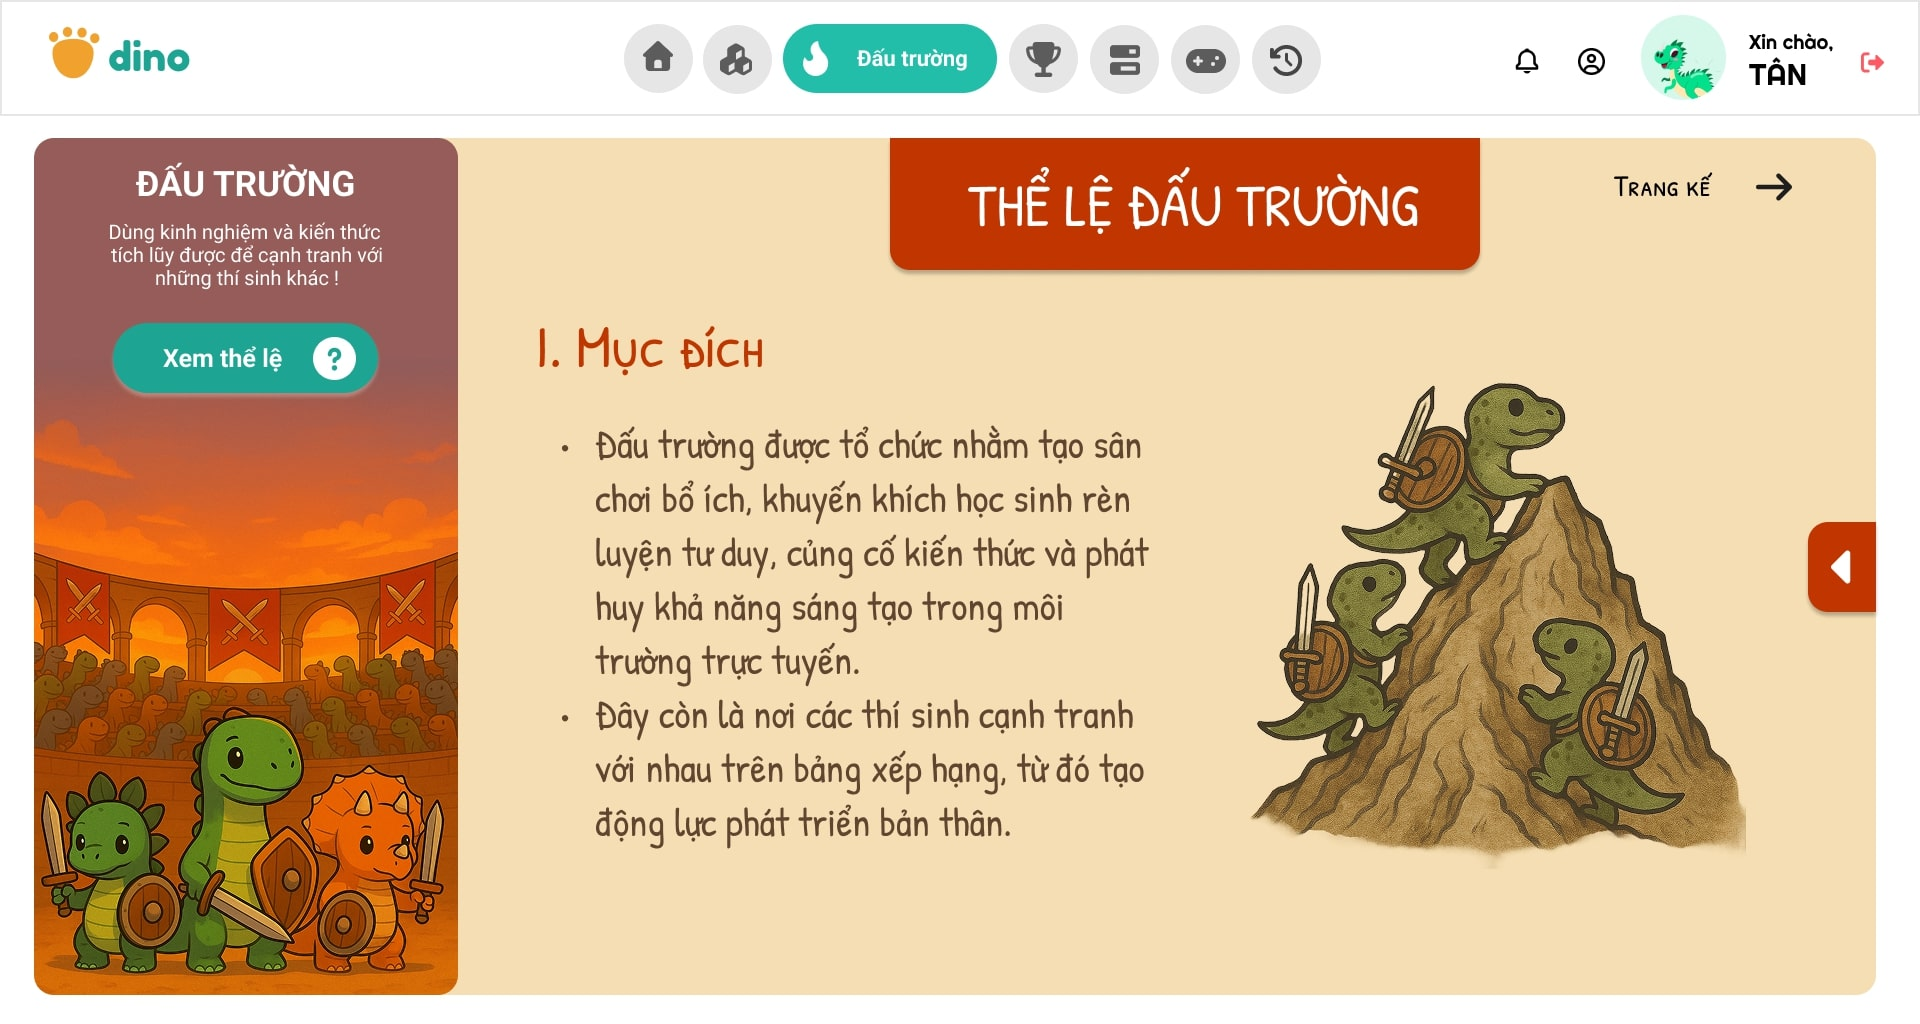
\includegraphics[width=0.48\textwidth]{Image/UI/Main-Student/Arena-R1.jpg}
		\hspace{0.1cm} % Đẩy hình 2 sang sát lề phải của minipage
		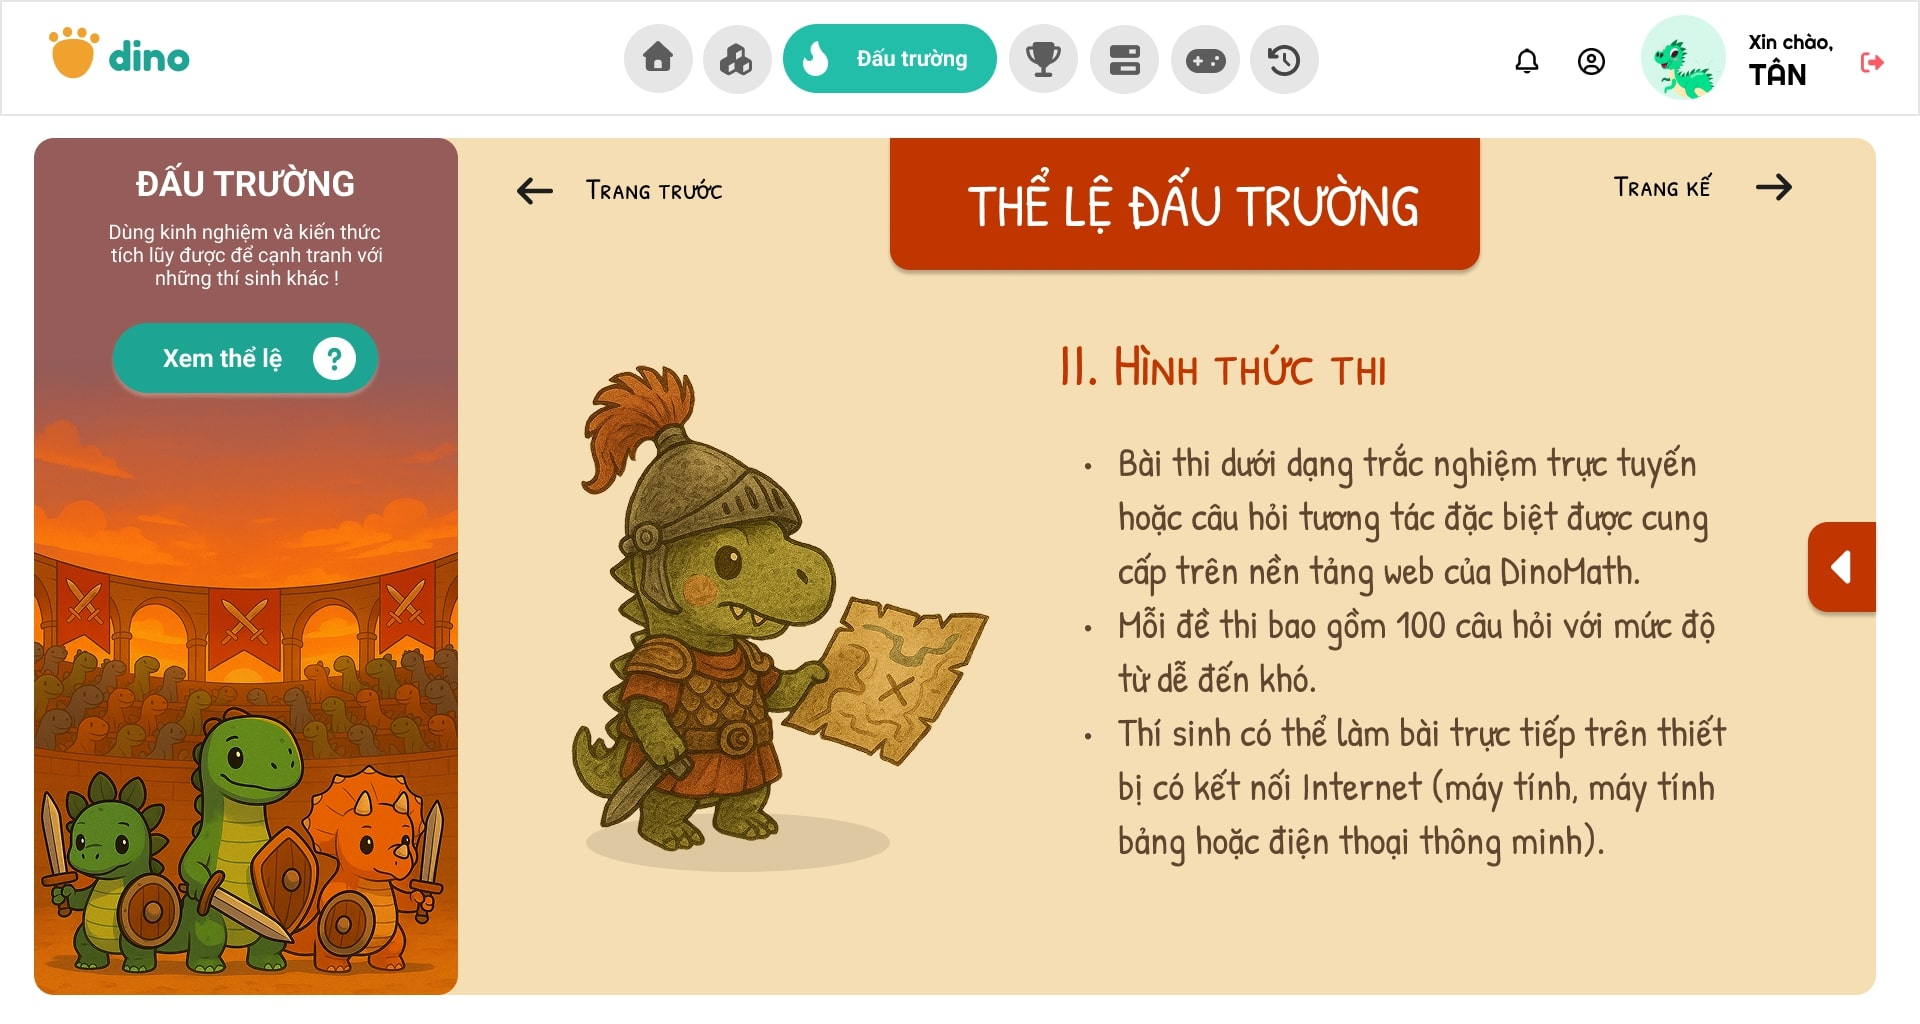
\includegraphics[width=0.48\textwidth]{Image/UI/Main-Student/Arena-R2.jpg}
		\\[0.3cm] % Khoảng cách dòng
		
		% Dòng 2
		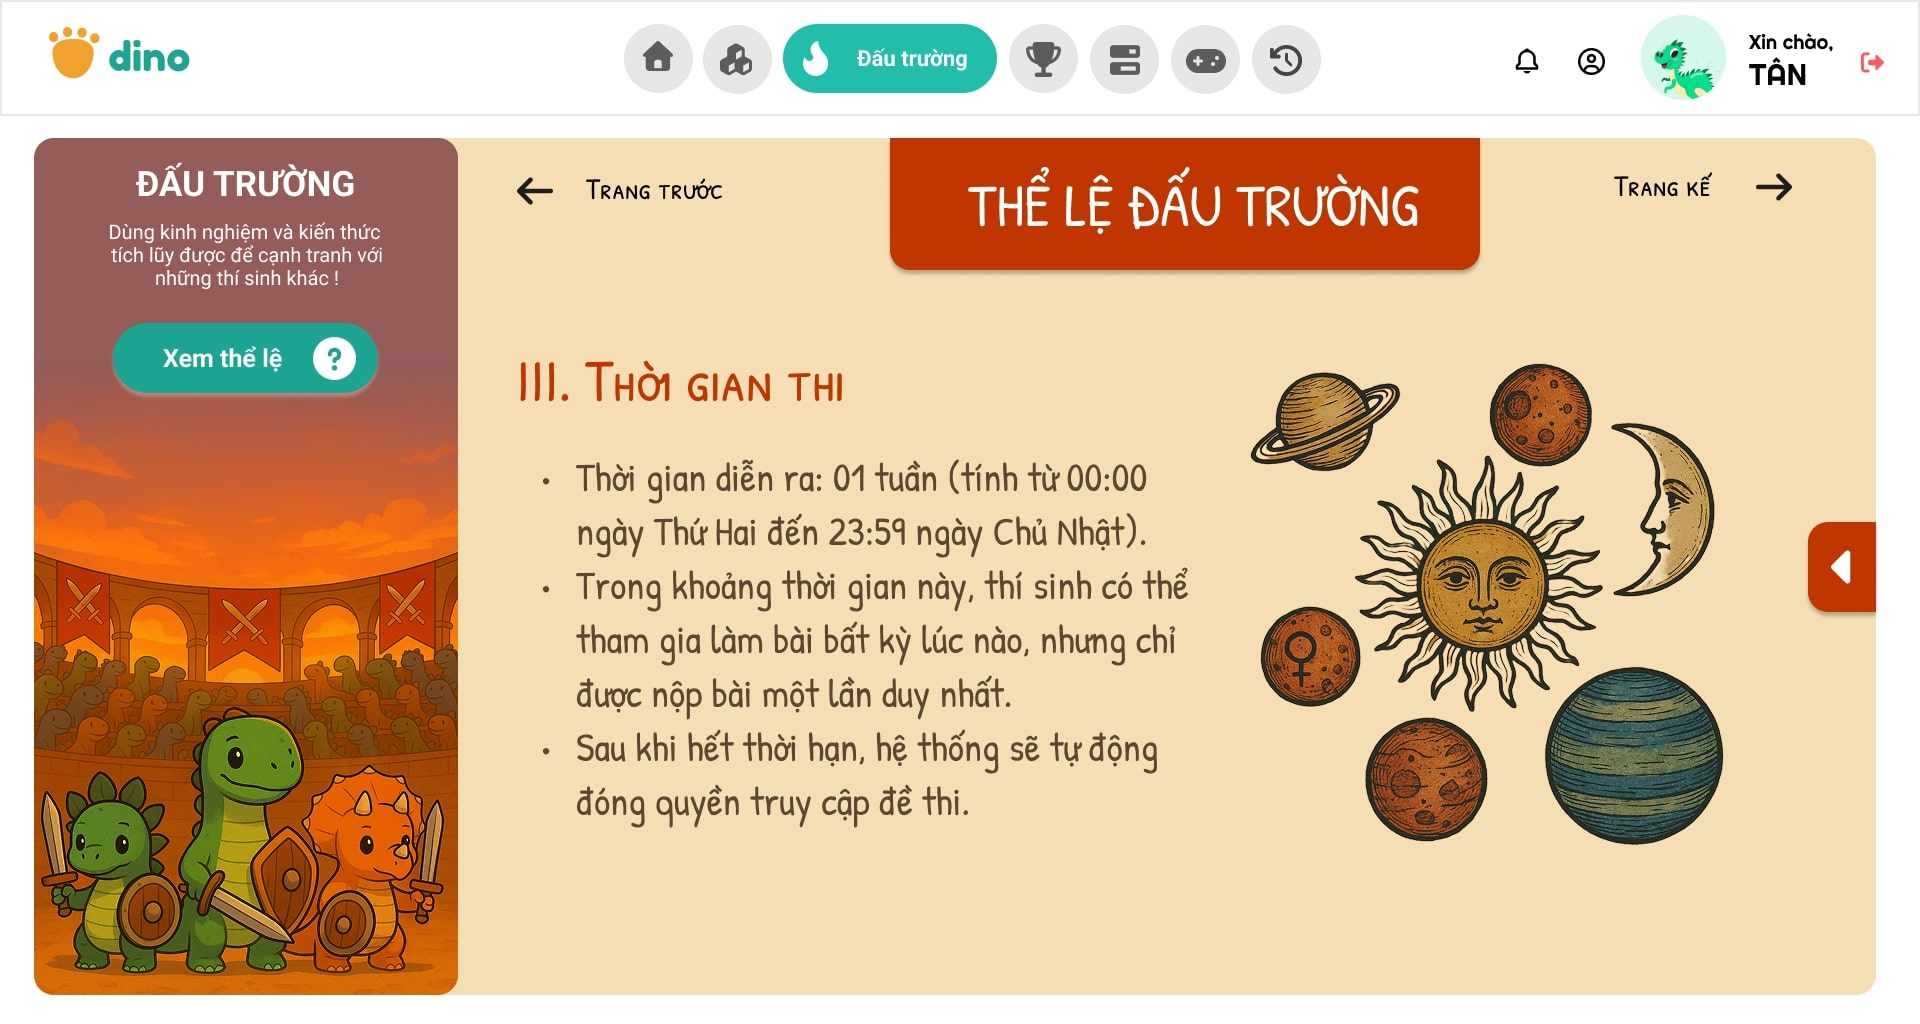
\includegraphics[width=0.48\textwidth]{Image/UI/Main-Student/Arena-R3.jpg}
		\hspace{0.1cm}
		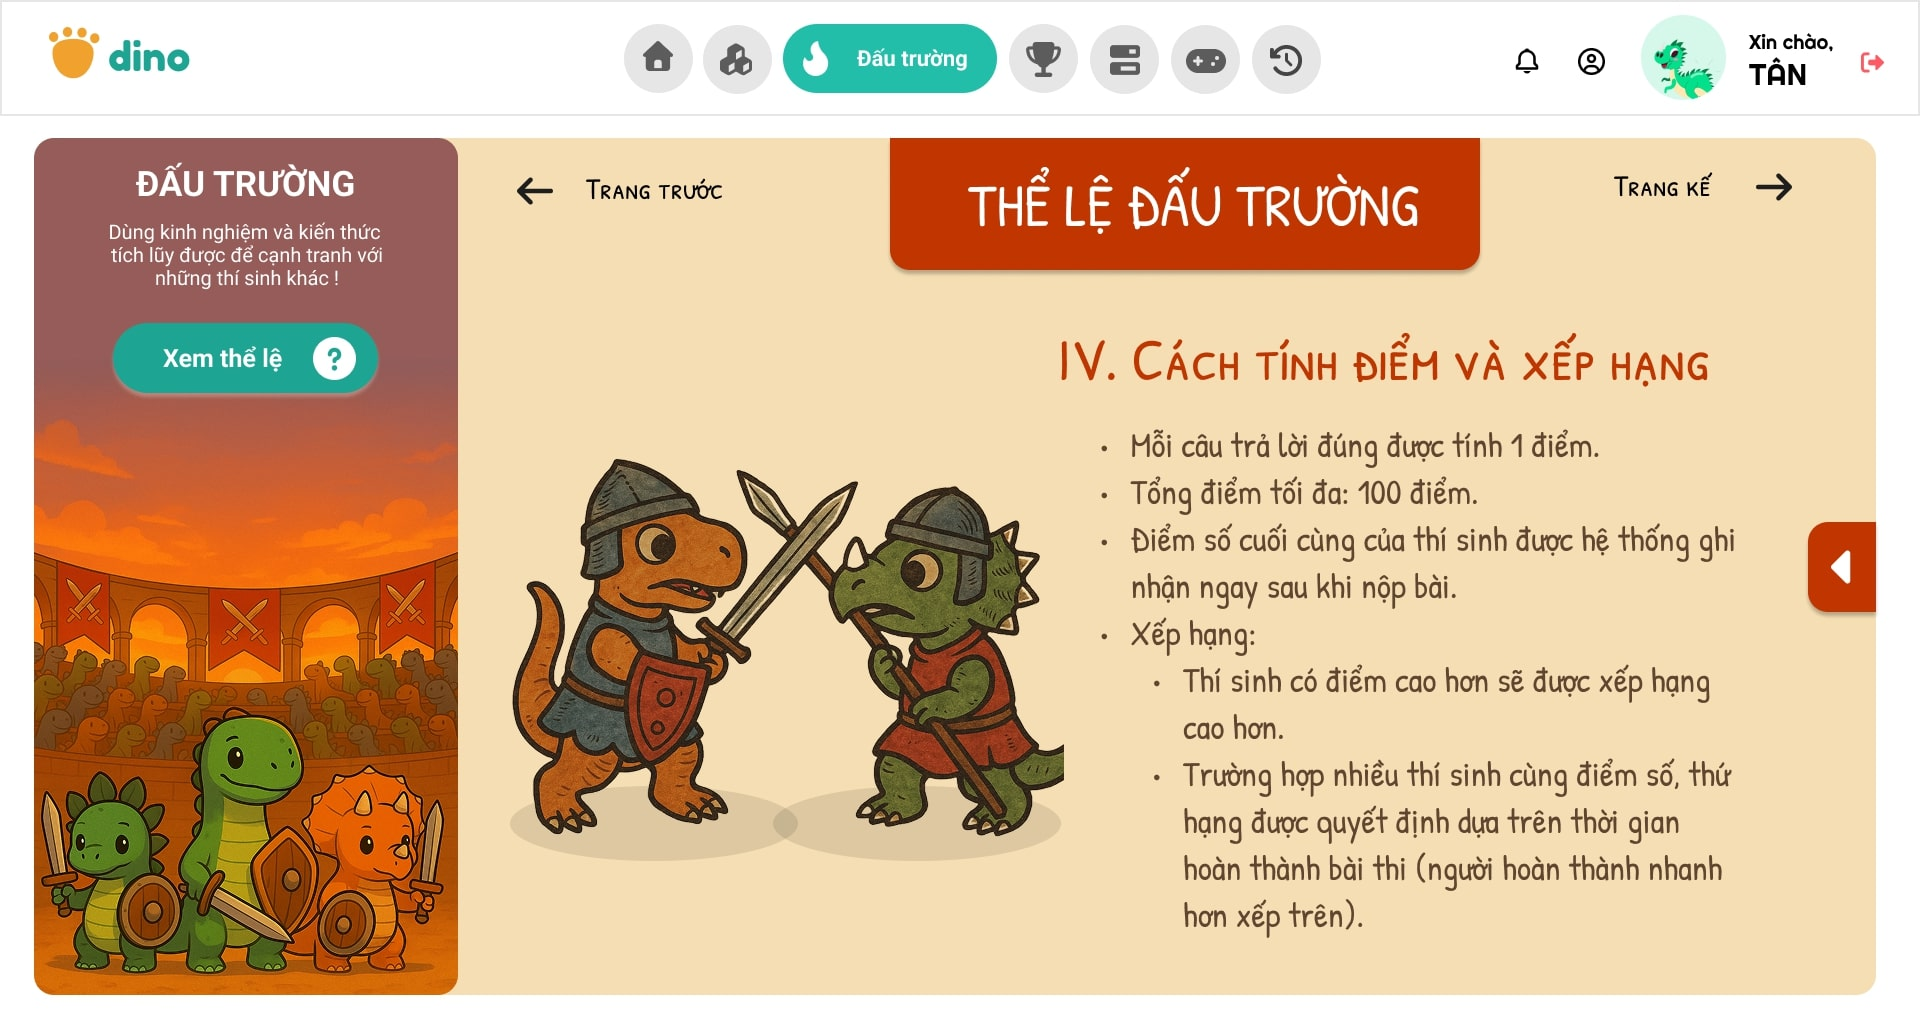
\includegraphics[width=0.48\textwidth]{Image/UI/Main-Student/Arena-R4.jpg}
		\\[0.3cm]
		
		% Dòng 3 (Hình cuối cùng nằm giữa hoặc căn trái tùy ý)
		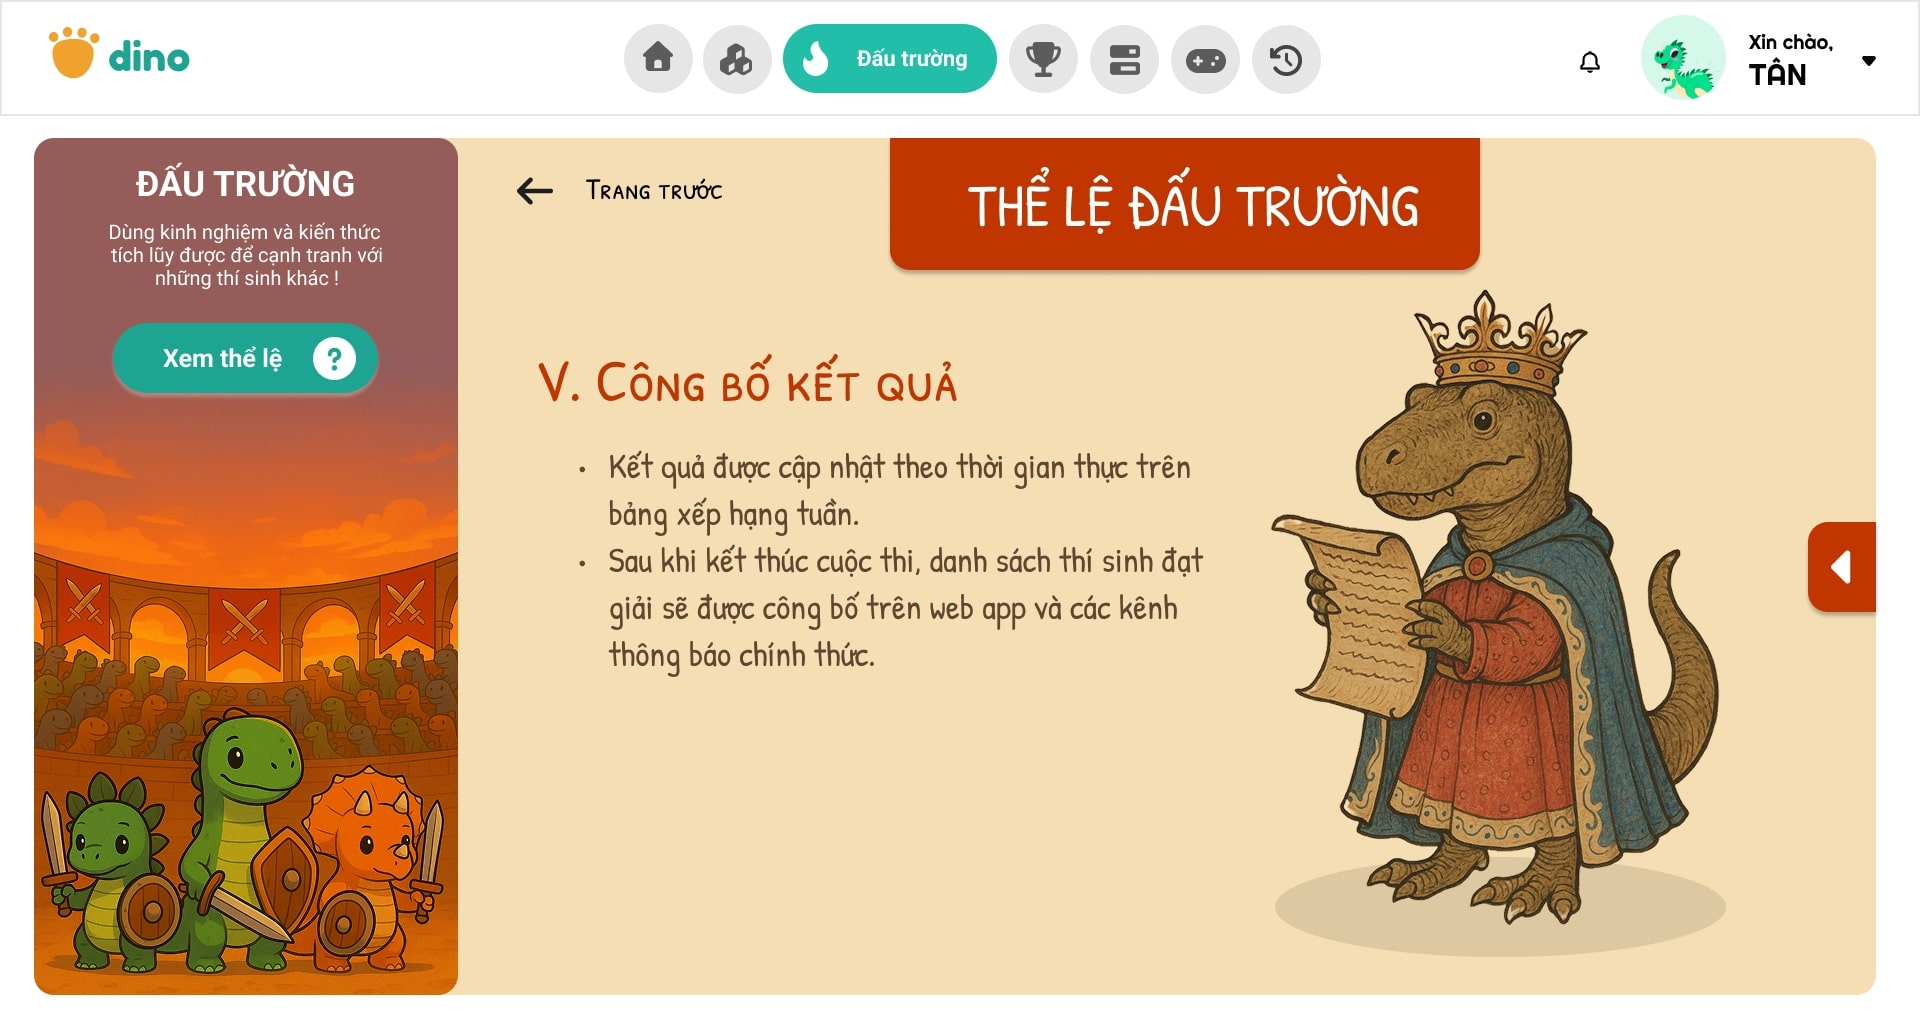
\includegraphics[width=0.48\textwidth]{Image/UI/Main-Student/Arena-R5.jpg}
		
	\end{minipage}
	\vspace{0.4cm}
	\caption{Trang Đấu trường - Thể lệ}
	\label{fig:arena-rules}
\end{figure}

Sau khi có kết quả bài thi Đấu trường, tùy theo số điểm đạt được mà mỗi thí sinh sẽ được thưởng một lượng Battle Points nhất định (đơn vị điểm dành riêng cho đấu trường). Battle Points (BP) sẽ là tiêu chí để xét xem một người dùng đang ở bậc xếp hạng nào. Các bậc xếp hạng và huy hiệu tương ứng được thiết kế như \textit{Hình \ref{fig:badges}}. Đối với bảng xếp hạng tuần, thứ hạng được quyết định dựa trên số điểm đạt được và thời gian hoàn thành bài thi của mỗi thí sinh.
	\begin{figure}[H]
		\centering
		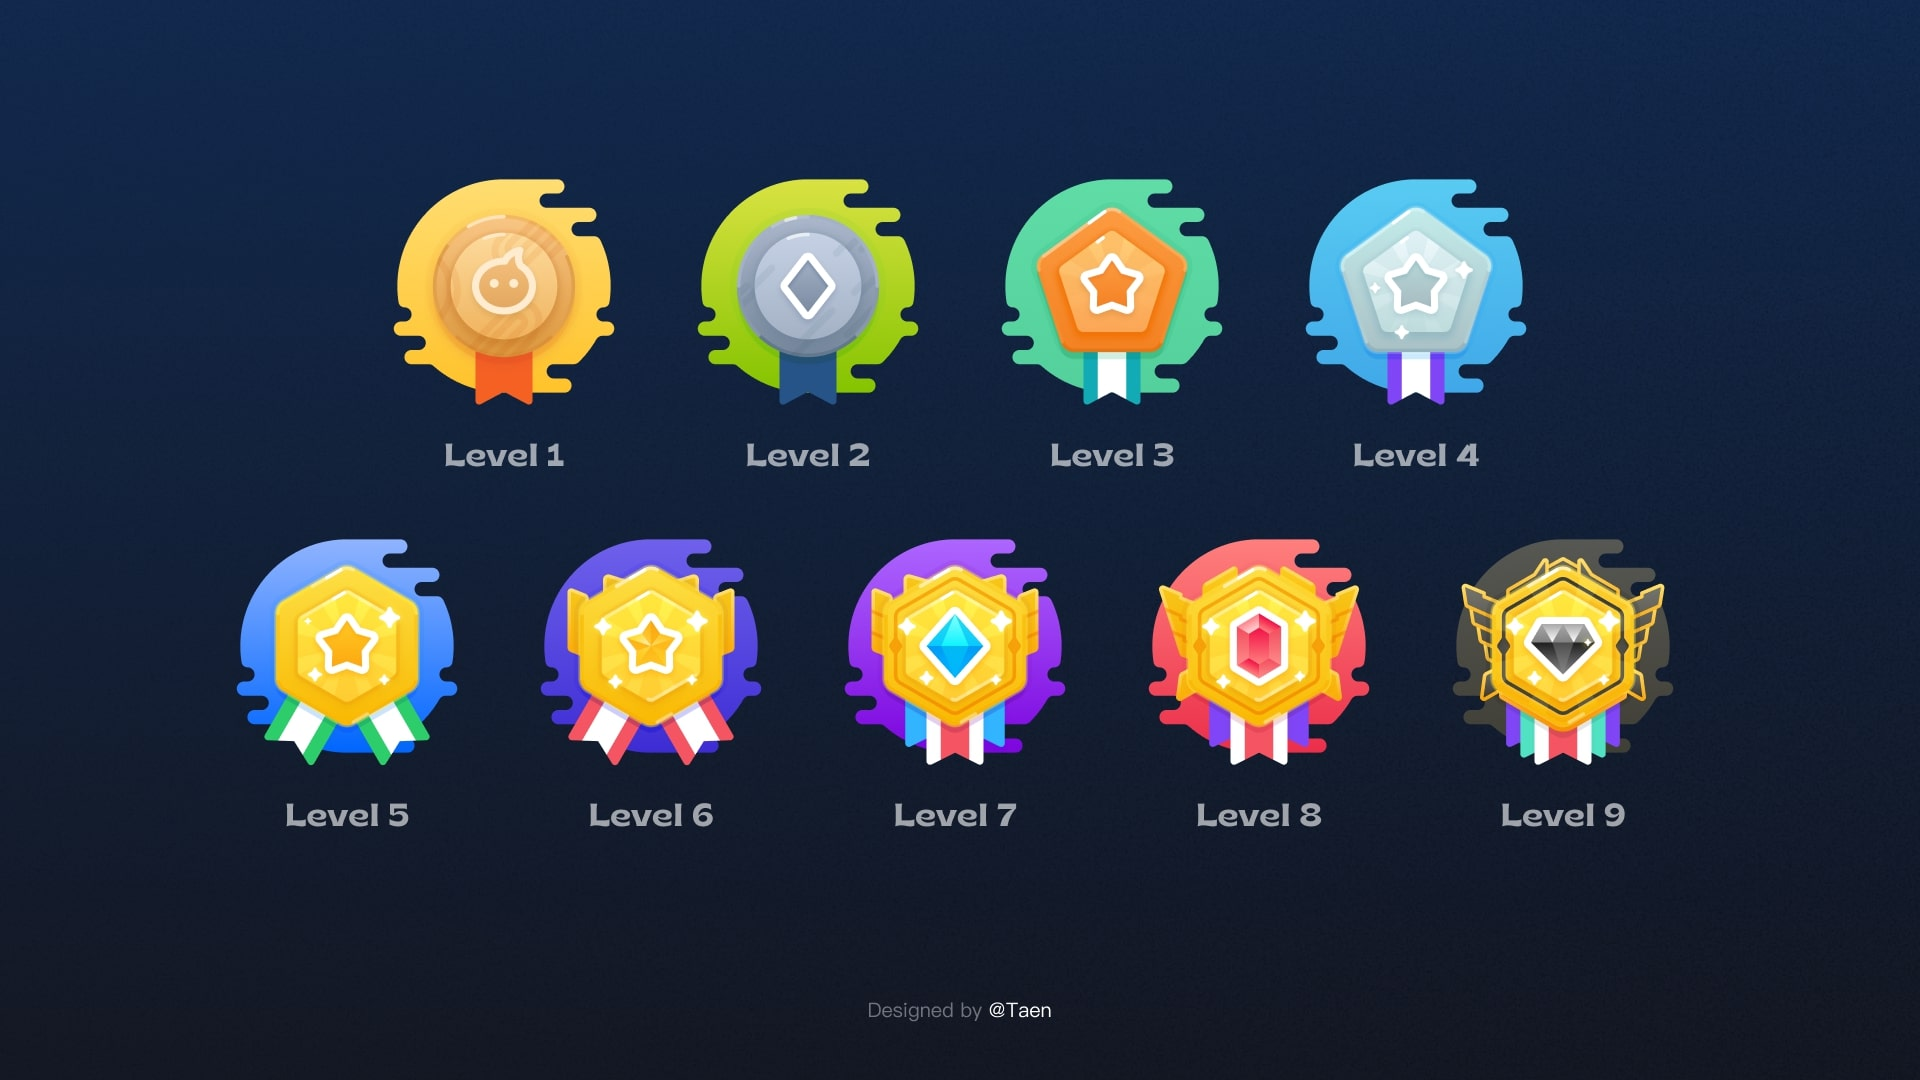
\includegraphics[width=0.9\textwidth]{Image/UI/badges.jpg}
		\vspace{0.6cm}
		\caption[
		Hệ thống các huy hiệu ứng với từng bậc xếp hạng
		]{
			\centering
			Hệ thống các huy hiệu ứng với từng bậc xếp hạng \\
			\textit{(nguồn: Rank Badge Design - Free by Taen \cite{figma_community_file})}
		}
		\label{fig:badges}
	\end{figure}
	
	
	\begin{figure}[H]
		\centering
		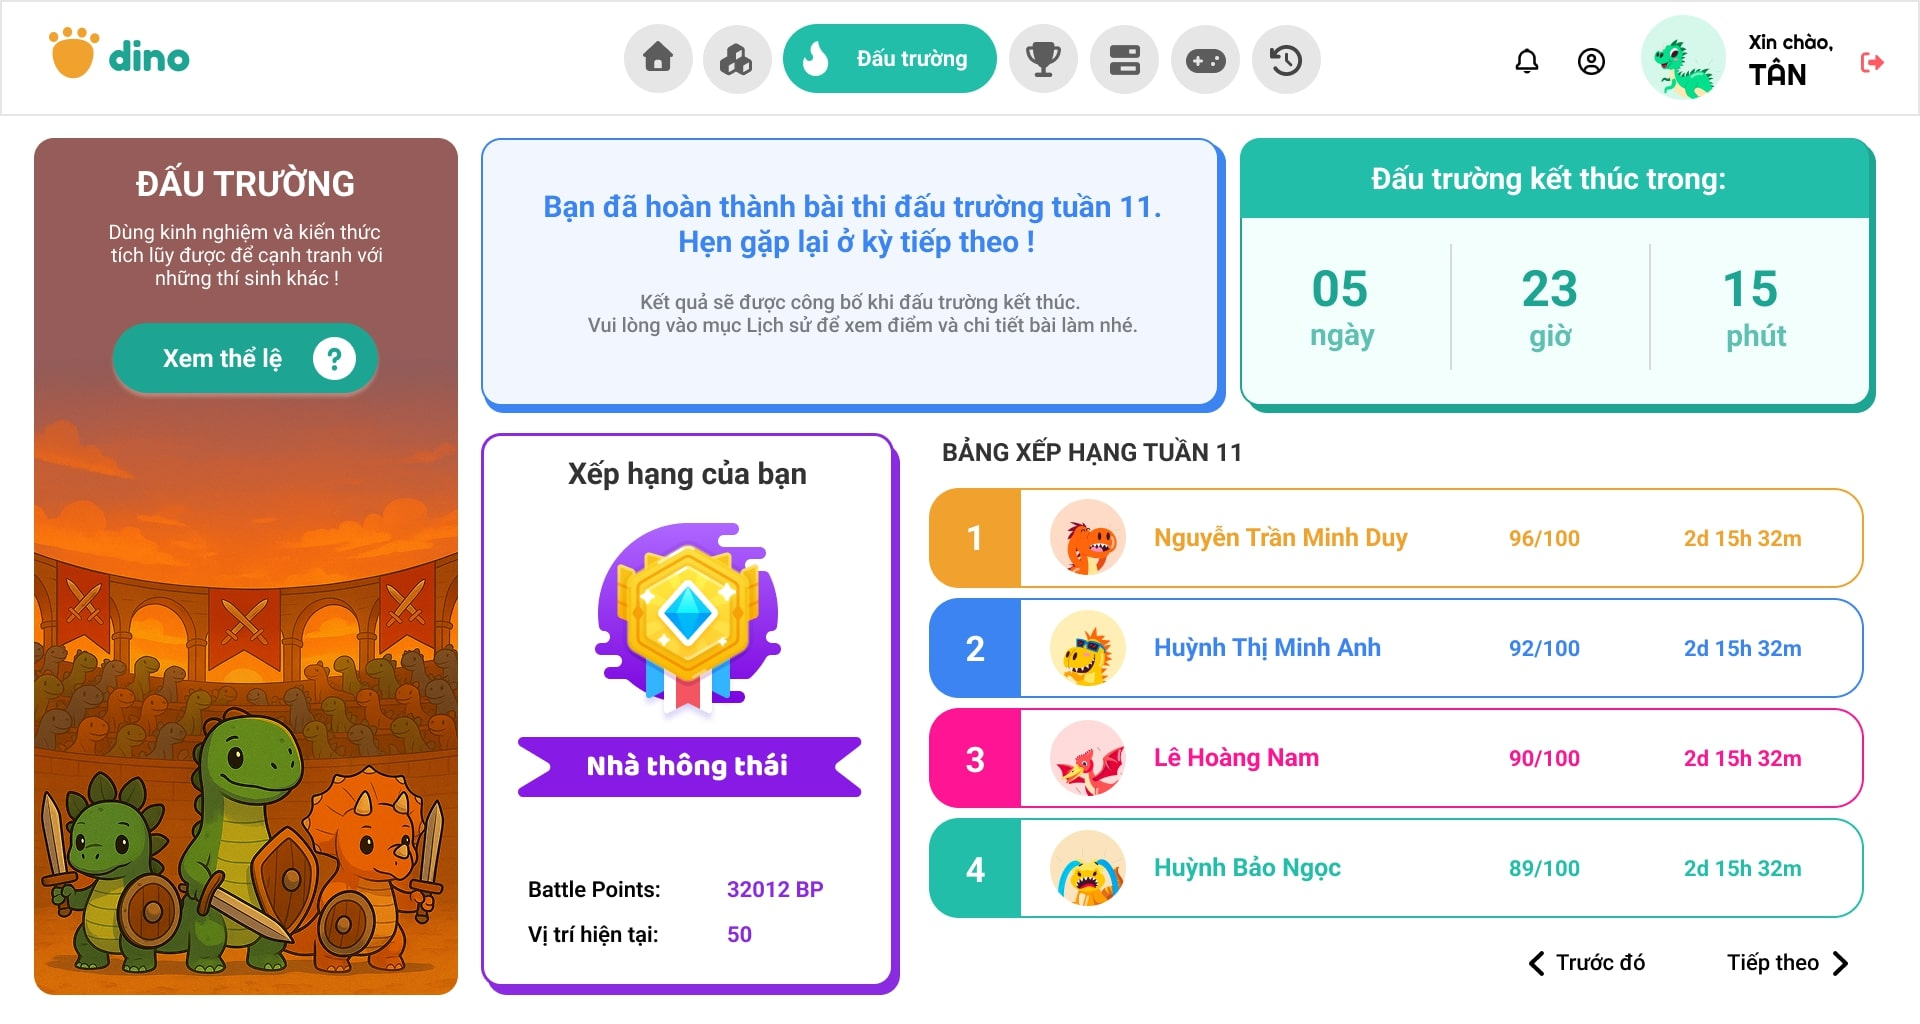
\includegraphics[width=0.9\textwidth]{Image/UI/Main-Student/Arena-Finished.jpg}
		\vspace{0.6cm}
		\caption{Trang Đấu trường - Sau khi hoàn thành bài thi}
	\end{figure}
\end{itemize}

\subsubsection{Trang Bài thi}
\label{subsubsec:exam}
\textbf{Trang Bài thi} cung cấp giao diện làm bài cho \textbf{Bài kiểm tra đầu vào} (mục \ref{subsubsec:studenthome}) và \textbf{Đấu trường} (mục \ref{subsubsec:arena}). Người dùng có thể chuyển câu hỏi bằng cách bấm vào các nút số ở thanh bên trái của màn hình hoặc bấm các nút điều hướng để chuyển sang câu tiếp theo hoặc trước đó. Giao diện còn hỗ trợ hiển thị thời gian làm bài còn lại cũng như số câu hỏi đã làm trên tổng số câu hỏi. Tất cả các câu hỏi kiểm tra sẽ thuộc dạng trắc nghiệm. Đối với bài thi Đấu trường, do thời gian làm bài dài (7 ngày), người dùng có thể thoát và lưu tiến trình làm bài của mình để có thể tiếp tục làm sau đó.
	\begin{figure}[H]
		\centering
		\begin{minipage}{0.45\textwidth}
			\centering
			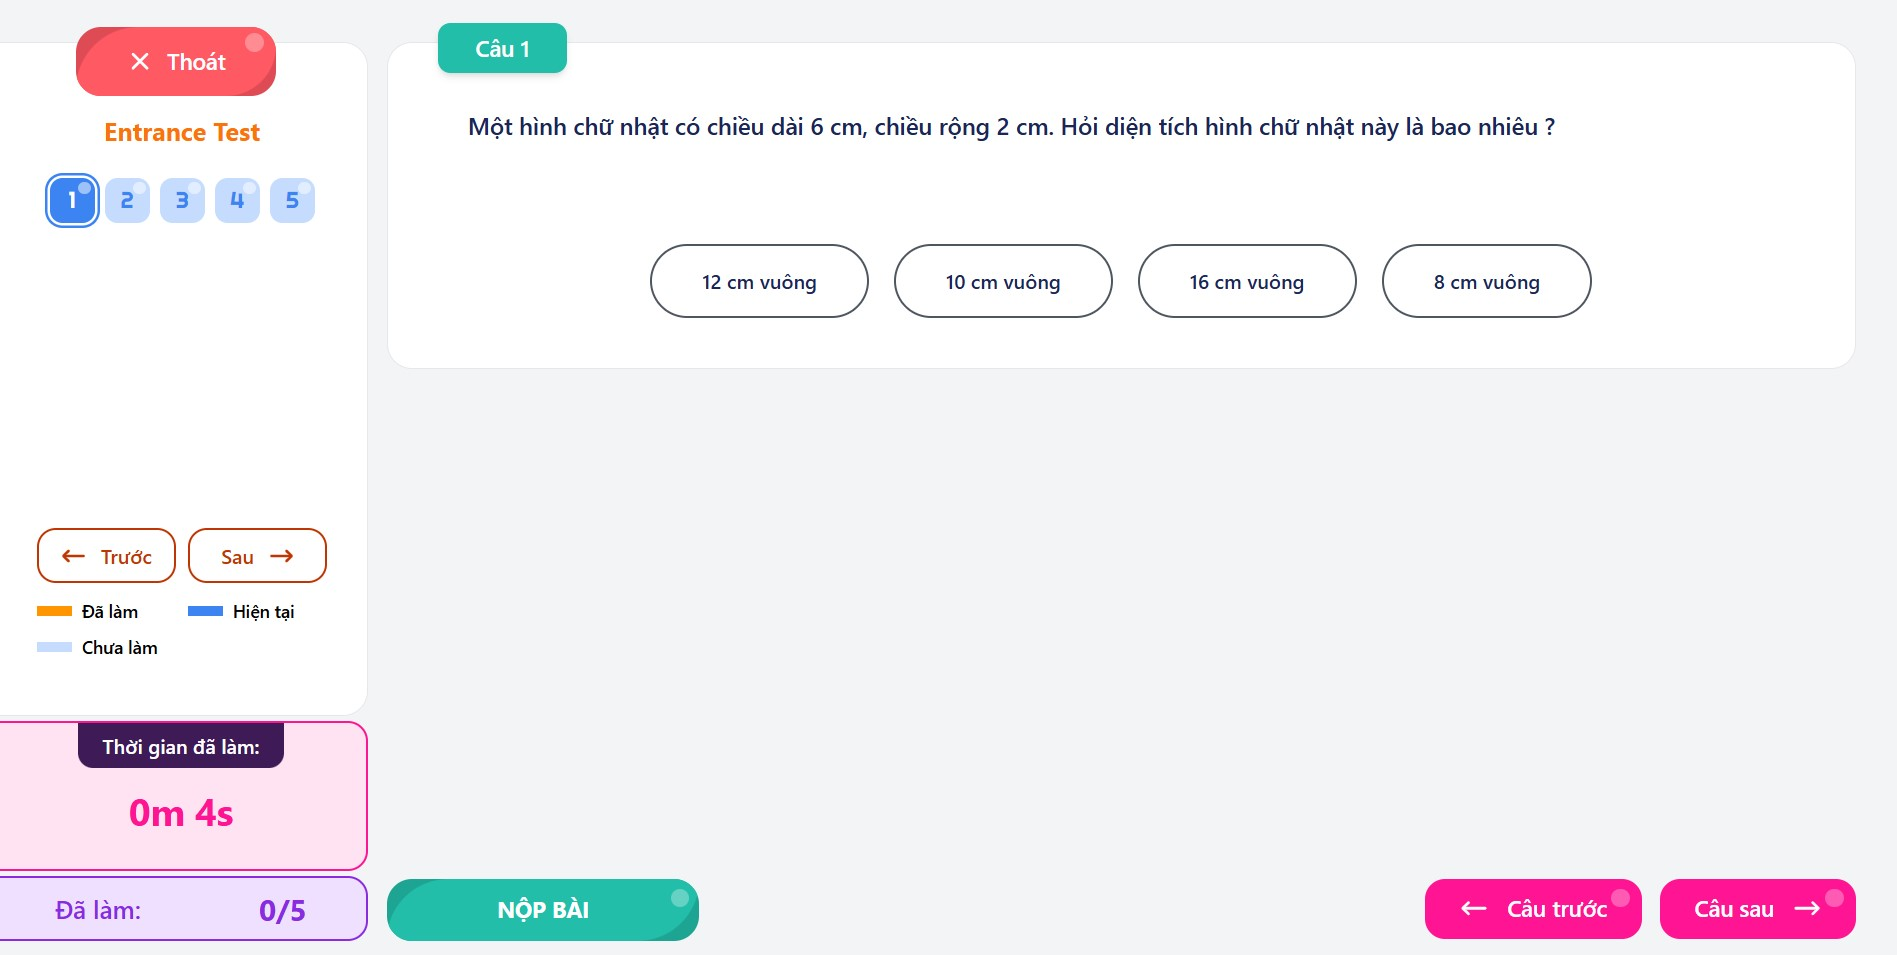
\includegraphics[width=\textwidth]{Image/UI/Main-Student/ExamChoices.jpg}
			\vspace{0.2cm}
			\caption{Dạng trắc nghiệm}
			\label{fig:exam1}
		\end{minipage}
		\hspace{0.1cm}
		\begin{minipage}{0.45\textwidth}
			\centering
			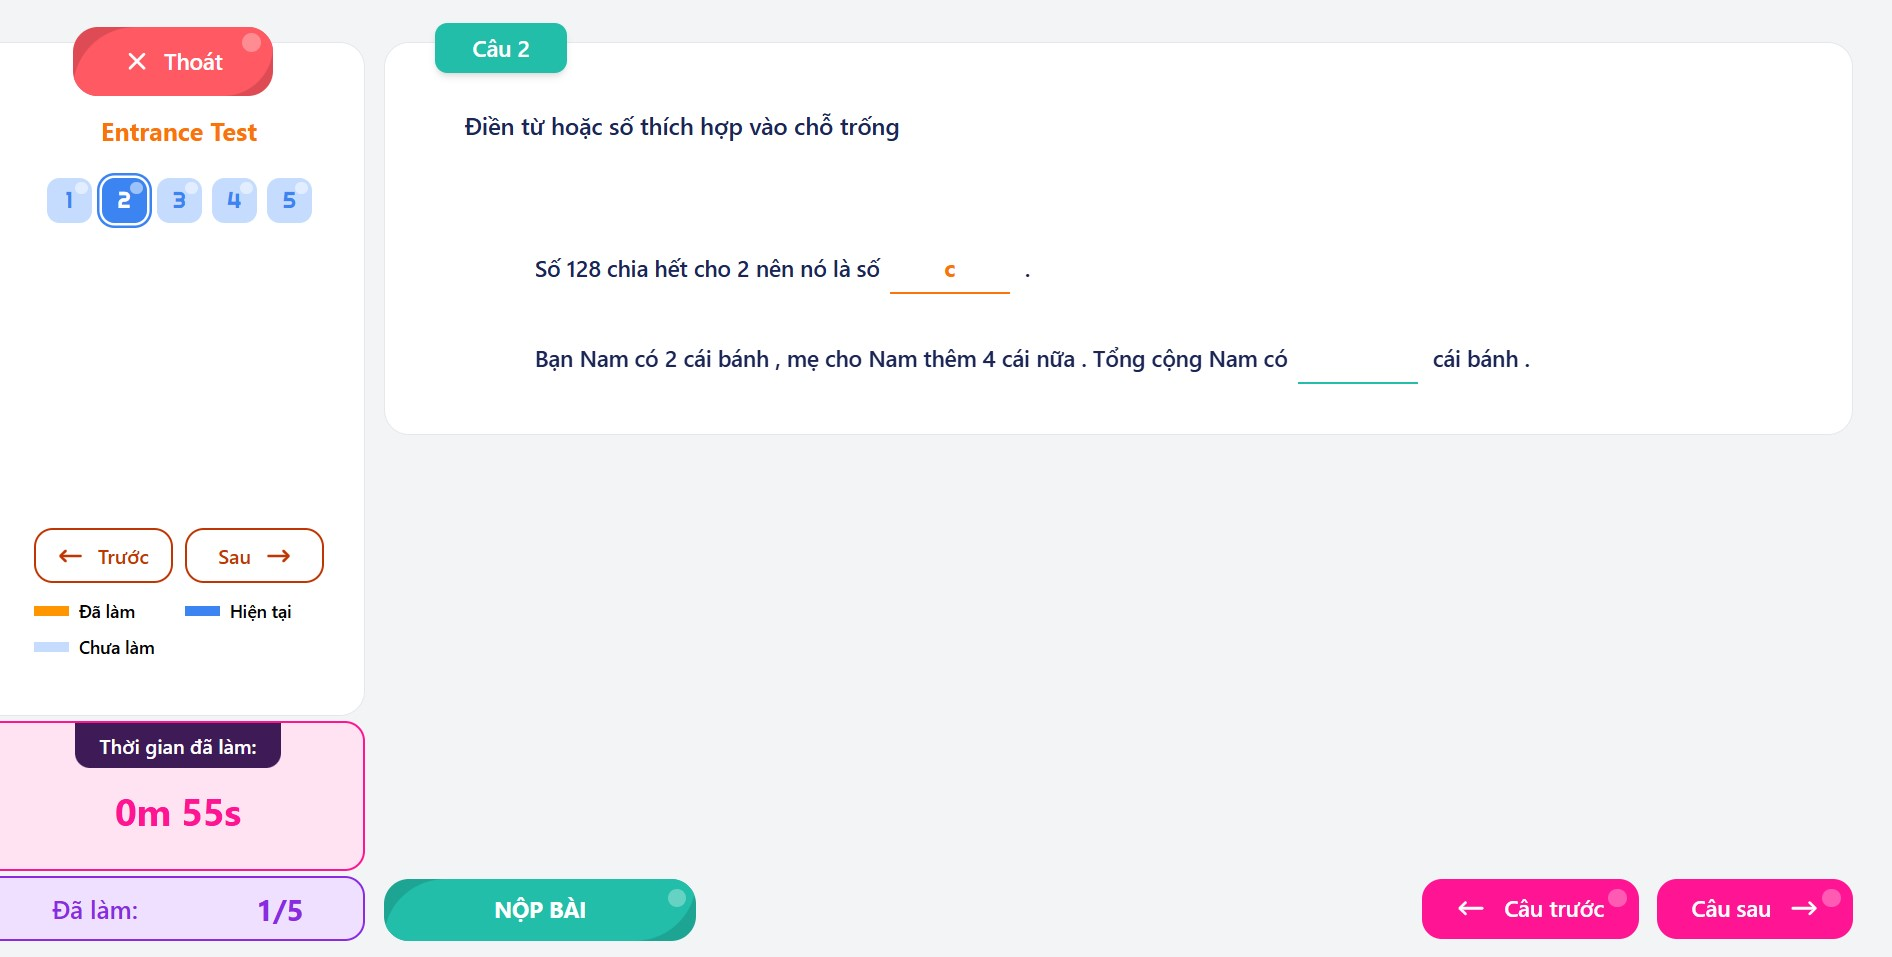
\includegraphics[width=\textwidth]{Image/UI/Main-Student/ExamFill.jpg}
			\vspace{0.2cm}
			\caption{Dạng điền khuyết}
			\label{fig:exam2}
		\end{minipage}
		
		\vspace{0.4cm}
		
		\begin{minipage}{0.45\textwidth}
			\centering
			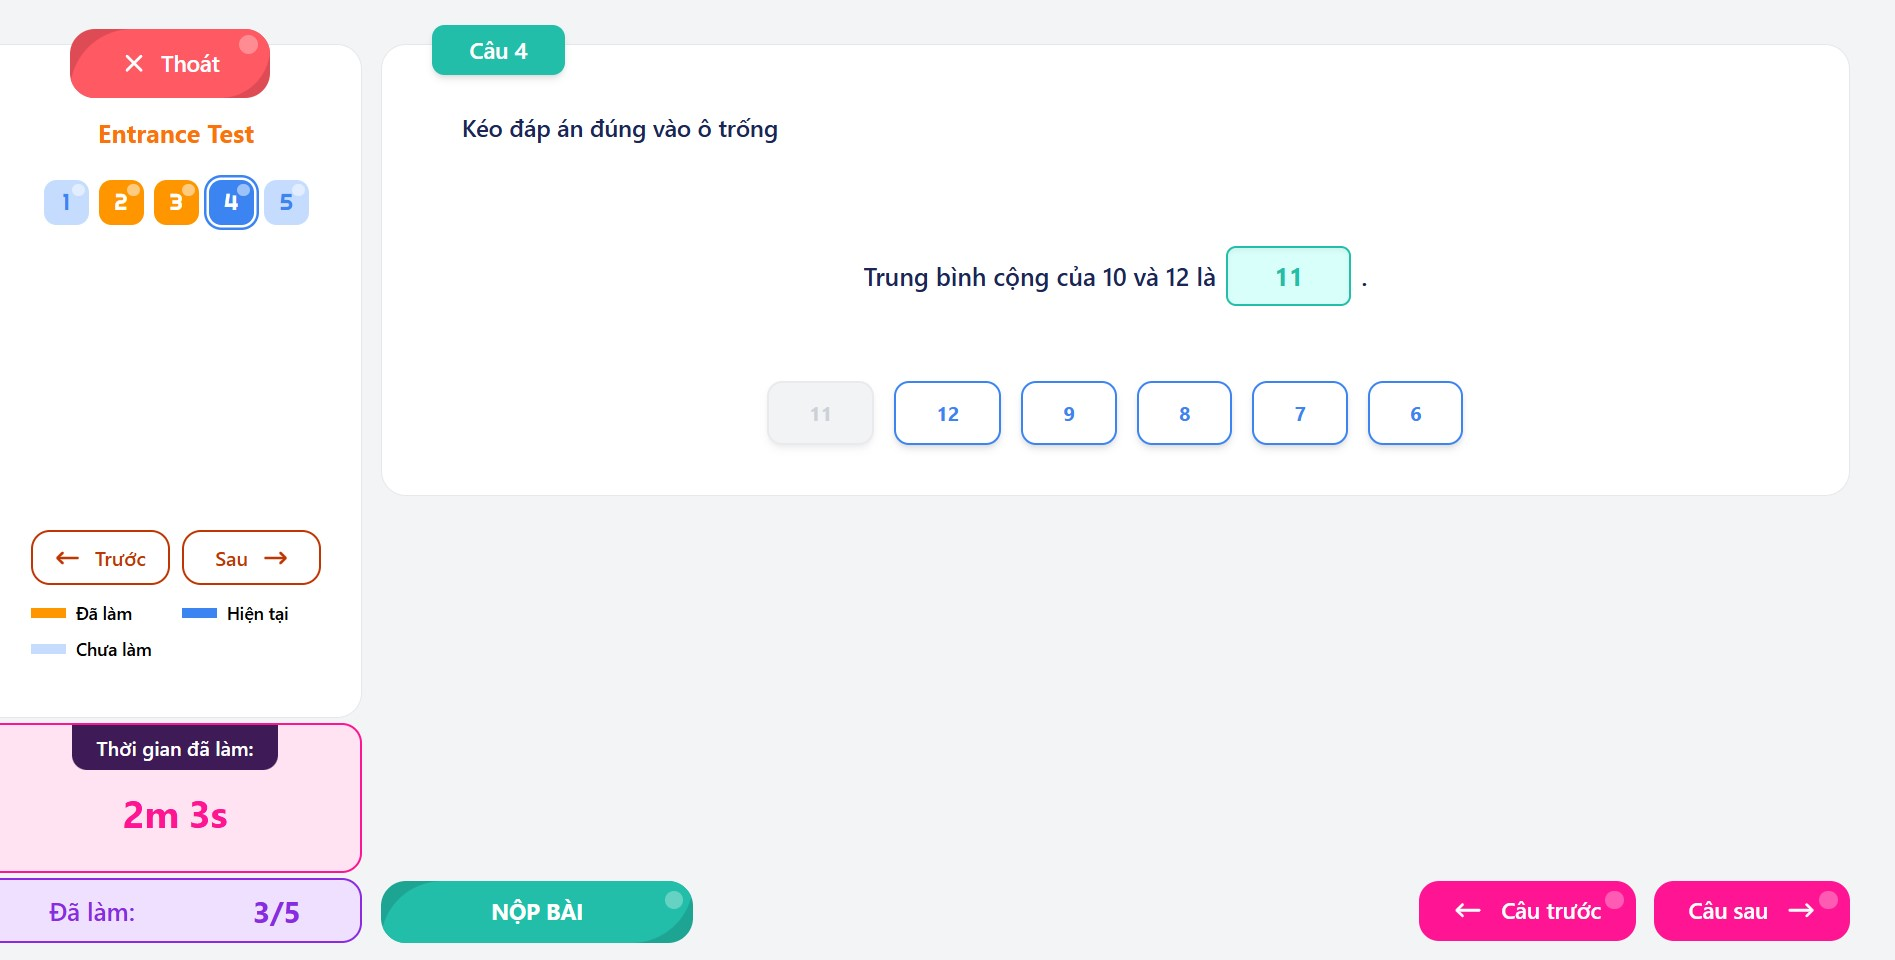
\includegraphics[width=\textwidth]{Image/UI/Main-Student/ExamFill2.jpg}
			\vspace{0.2cm}
			\caption{Dạng điền khuyết - Click to Fill}
			\label{fig:exam3}
		\end{minipage}
		\hspace{0.1cm}
		\begin{minipage}{0.45\textwidth}
			\centering
			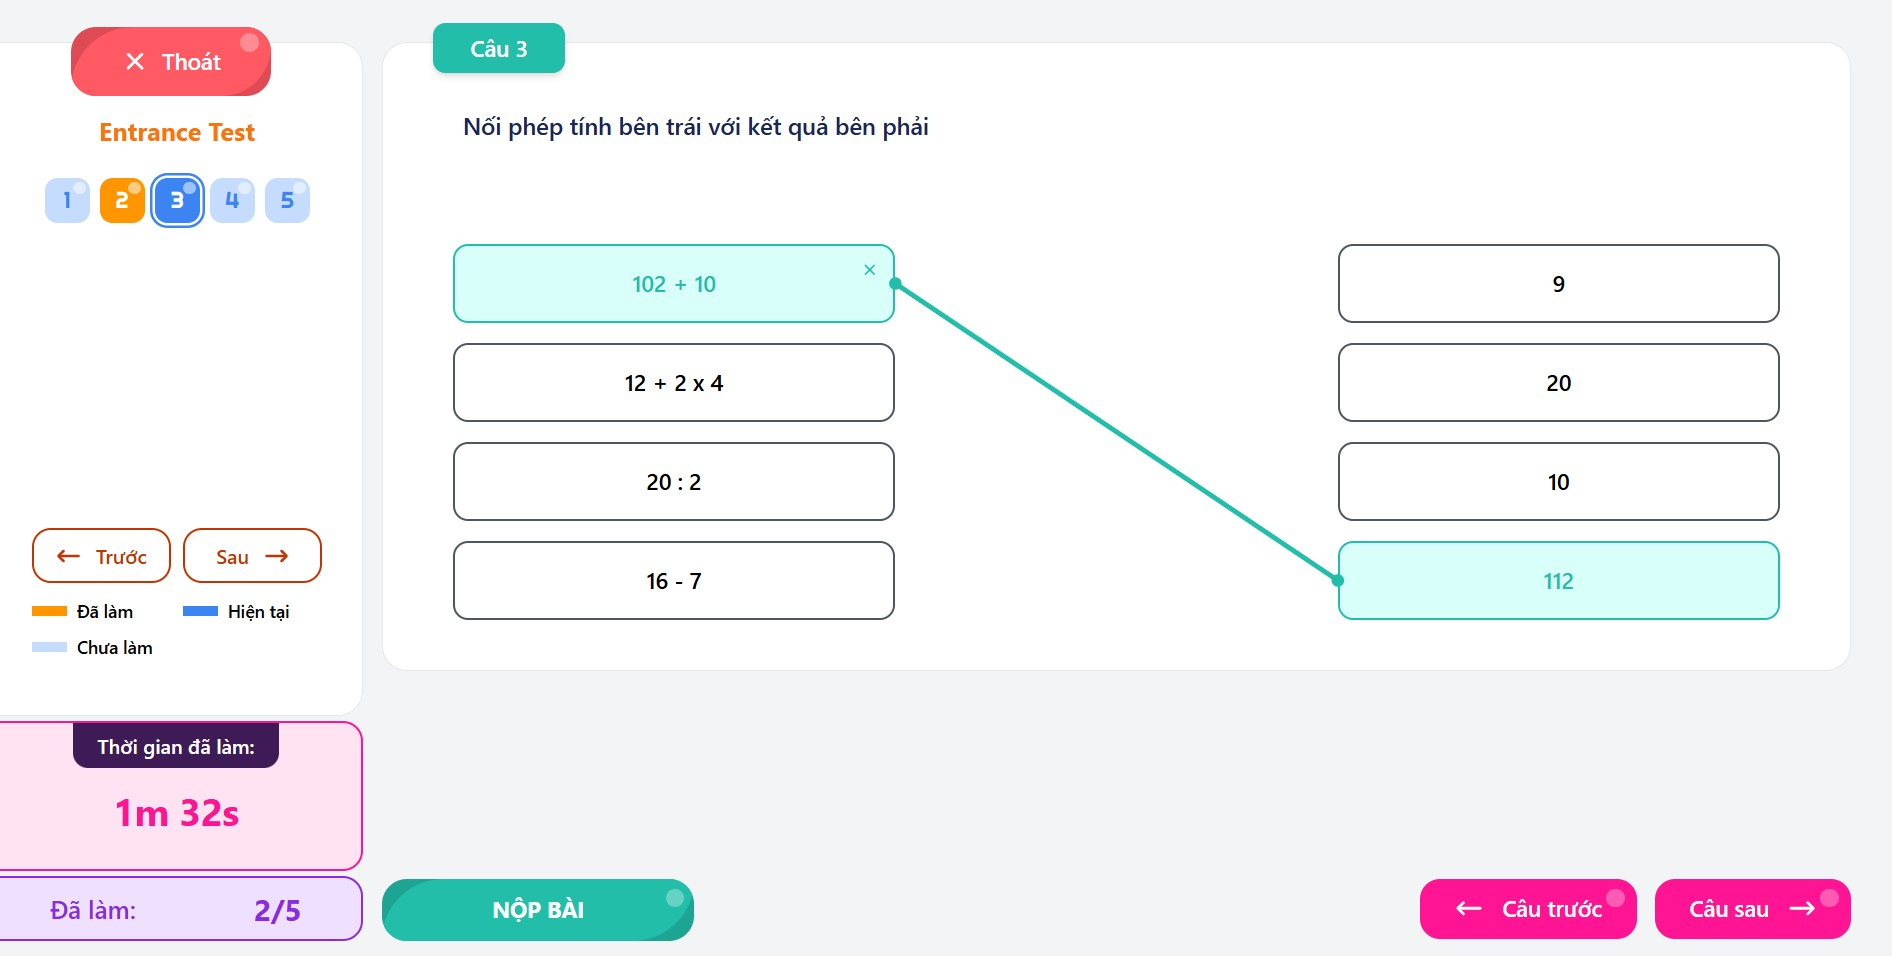
\includegraphics[width=\textwidth]{Image/UI/Main-Student/ExamMatching.jpg}
			\vspace{0.2cm}
			\caption{Dạng nối}
			\label{fig:exam4}
		\end{minipage}
		
		\vspace{0.4cm}
		
		\begin{minipage}{0.45\textwidth}
			\centering
			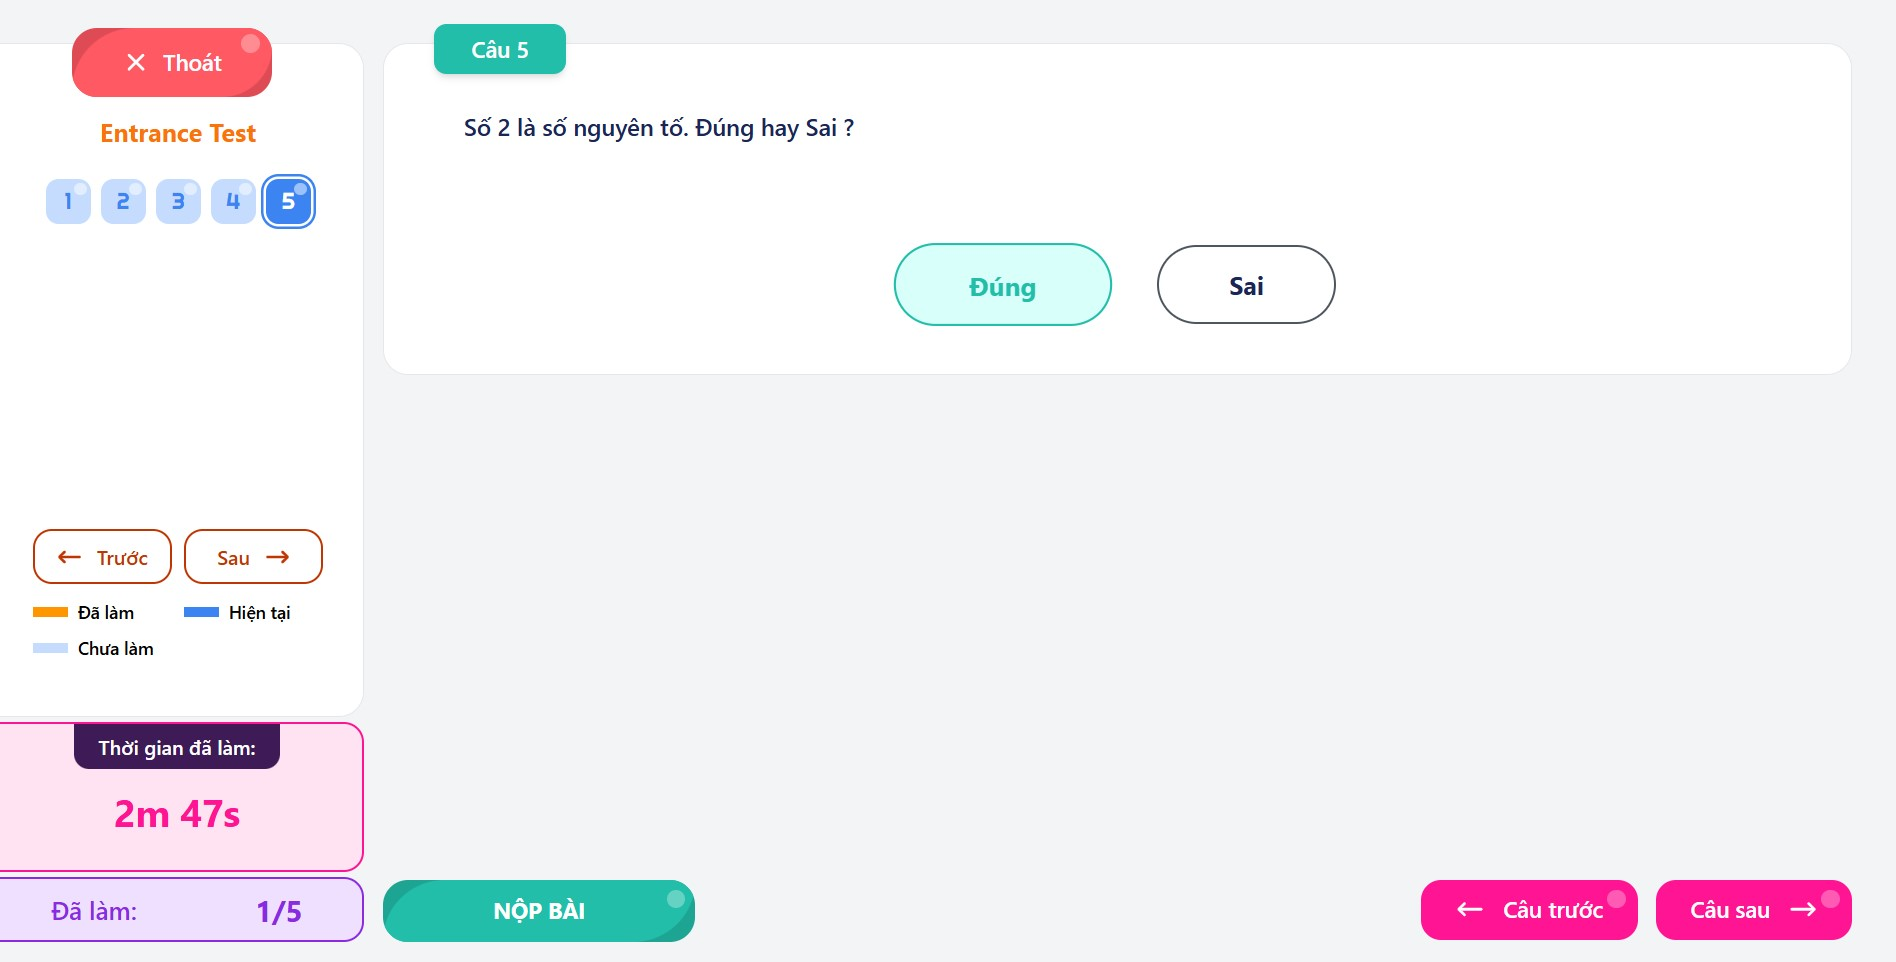
\includegraphics[width=\textwidth]{Image/UI/Main-Student/ExamTF.jpg}
			\vspace{0.2cm}
			\caption{Dạng đúng/sai}
			\label{fig:exam5}
		\end{minipage}
	\end{figure}
	
	\vspace{0.4cm}
\newline
Khi người dùng chưa hoàn thành bài thi nhưng bấm thoát, giao diện sẽ hiển thị một thông báo lưu tiến trình làm bài như \textit{Hình \ref{fig:save}}. Khi người dùng bấm nộp bài, giao diện sẽ hiển thị thông báo để xác nhận như \textit{Hình \ref{fig:submit}}.
	\begin{figure}[H]
		\centering
		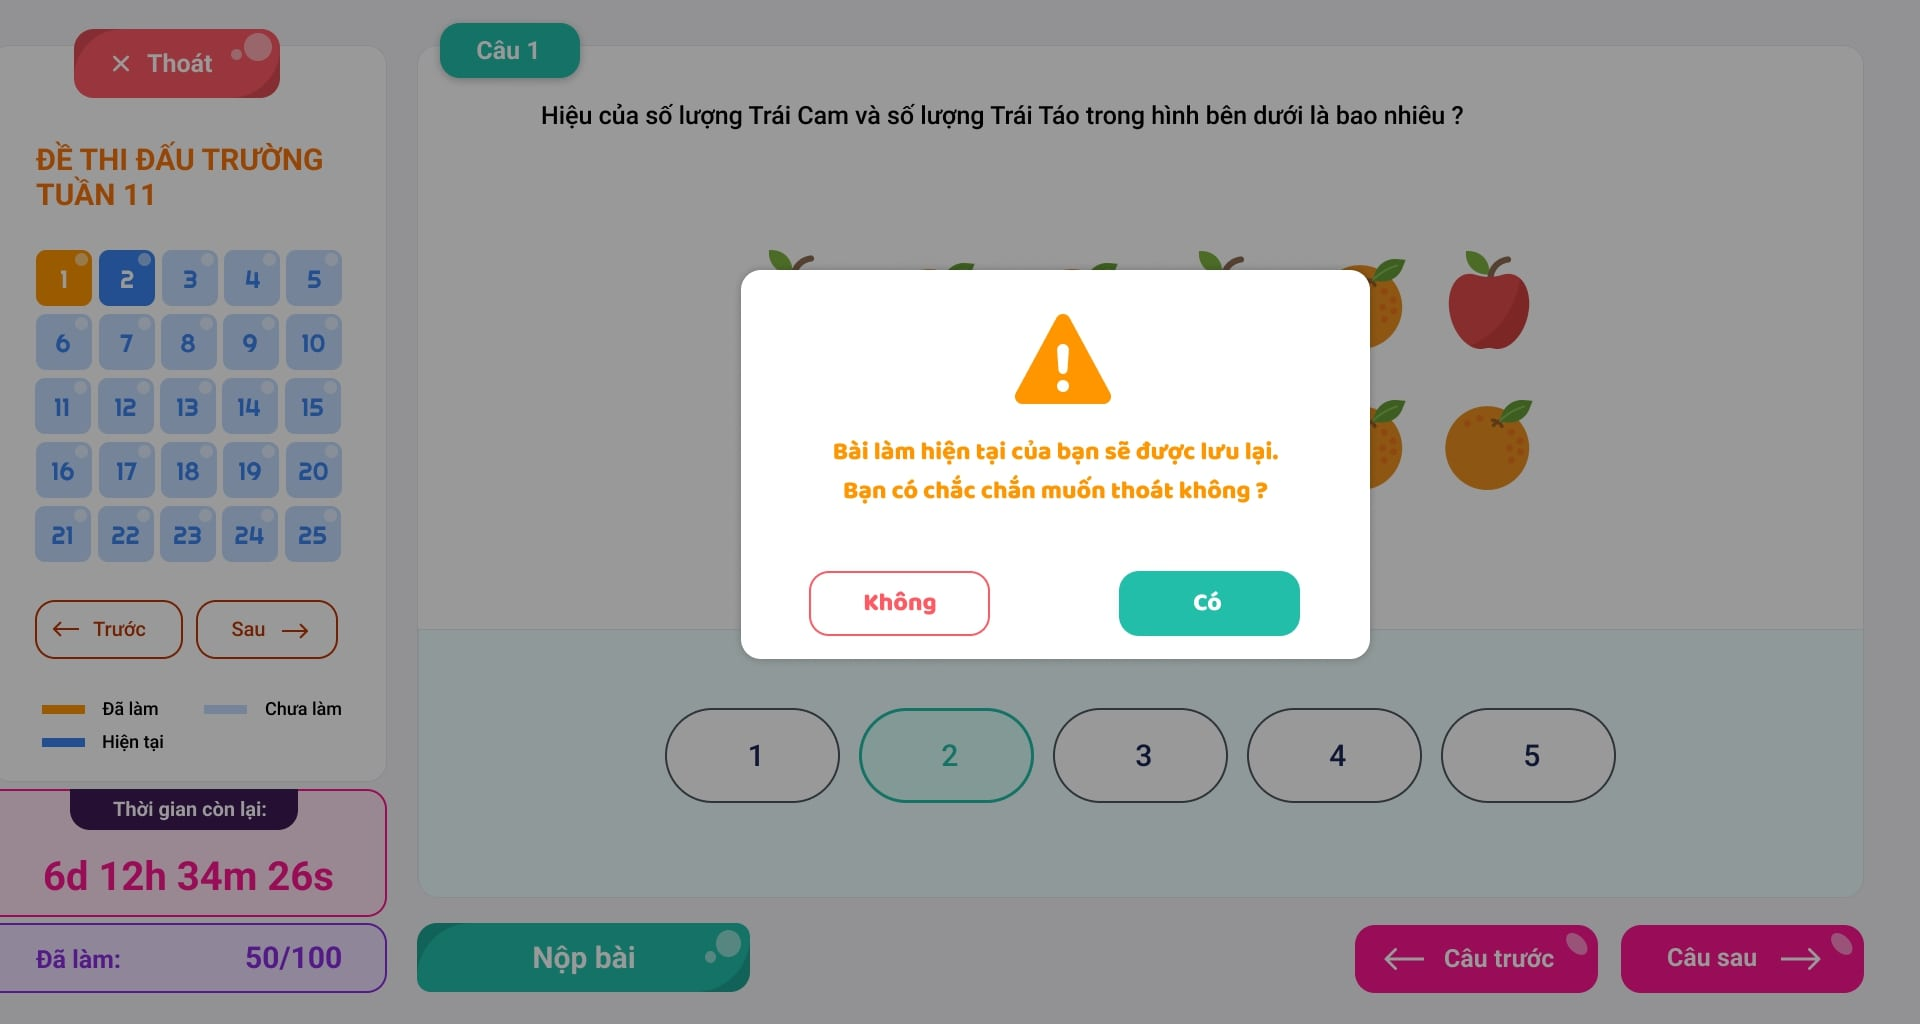
\includegraphics[width=0.9\textwidth]{Image/UI/Main-Student/Exitpopup.jpg}
		\vspace{0.6cm}
		\caption{Trang Bài thi - Thông báo khi thoát}
		\label{fig:save}
	\end{figure}
	\begin{figure}[H]
		\centering
		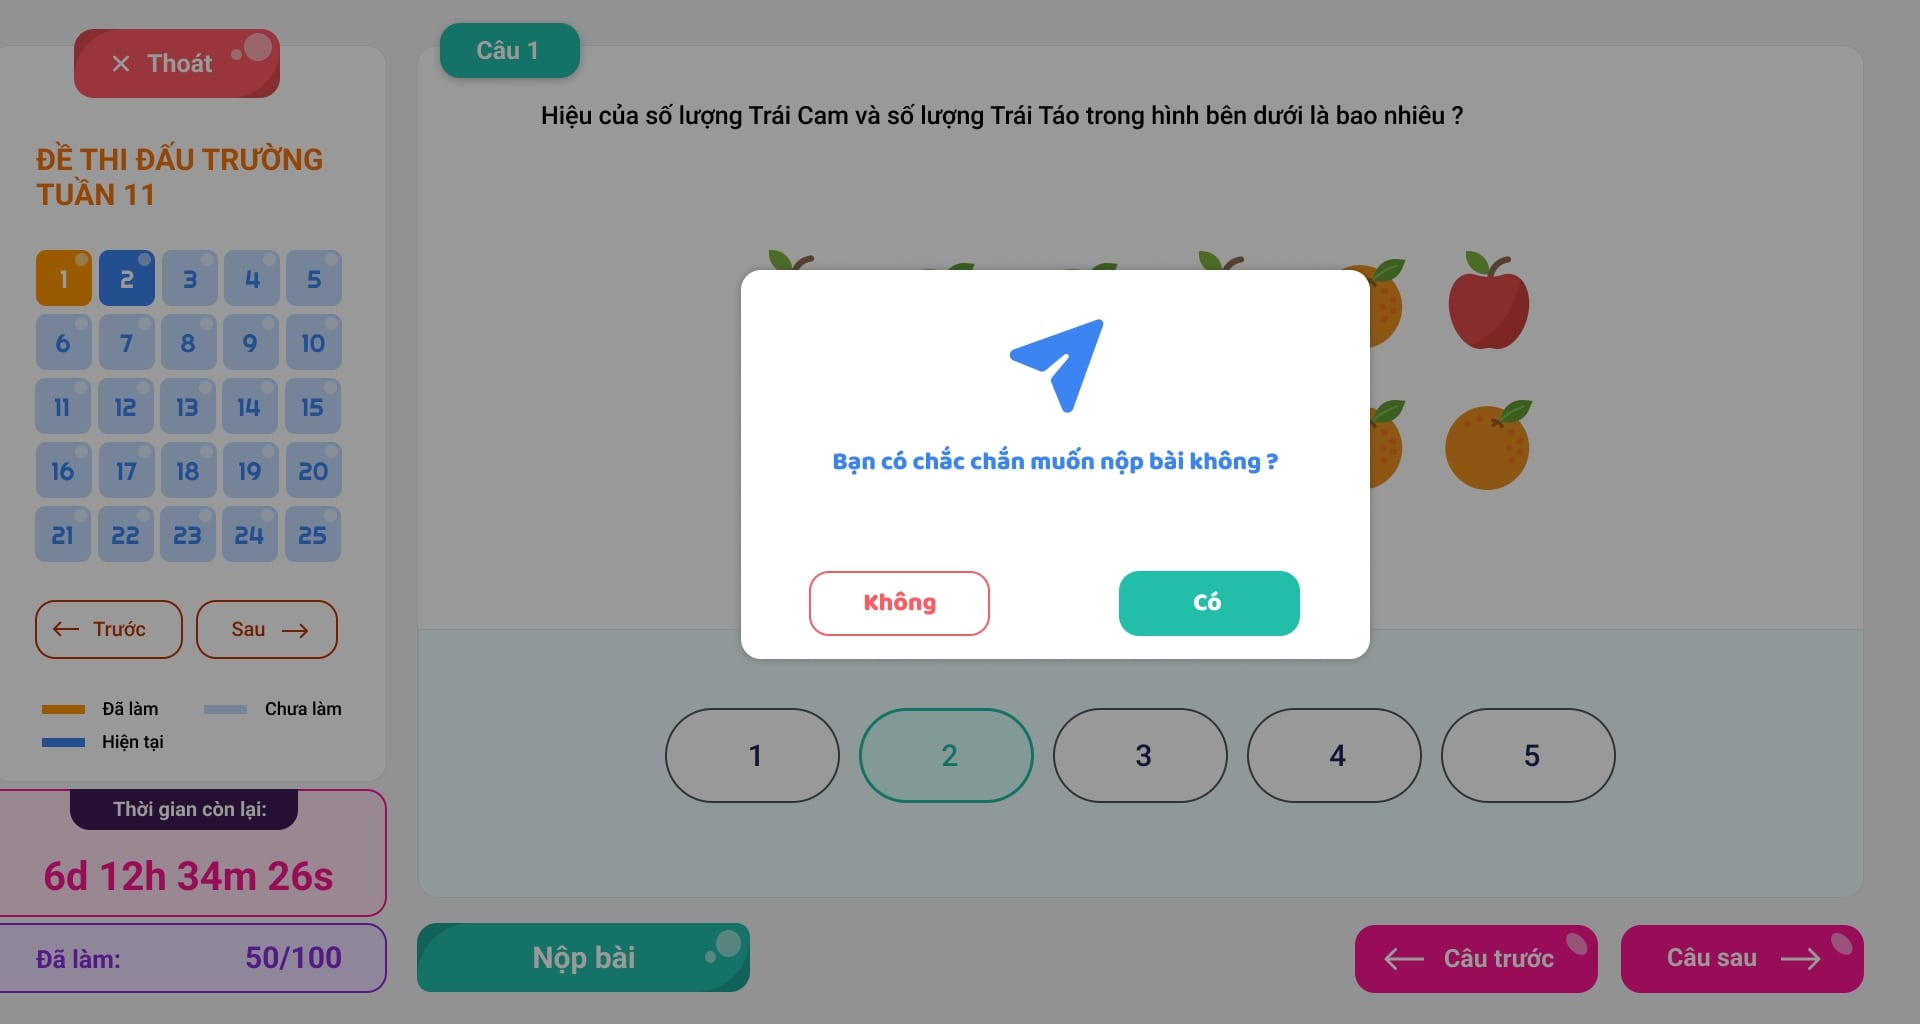
\includegraphics[width=0.9\textwidth]{Image/UI/Main-Student/Submitpopup.jpg}
		\vspace{0.6cm}
		\caption{Trang Bài thi - Thông báo khi bấm nộp bài}
		\label{fig:submit}
	\end{figure}

\subsubsection{Trang Xếp hạng}
Trang xếp hạng sẽ hiển thị top 8 học sinh đạt số lượng thạch anh cao nhất (thạch anh là tiêu chí để xếp hạng học tập), đồng thời vinh danh 3 học sinh xuất sắc nhất. Ngoài ra, trang còn hiển thị số lượng thạch anh mà người dùng đang sở hữu và vị trí xếp hạng hiện tại của người dùng.
	\begin{figure}[H]
		\centering
		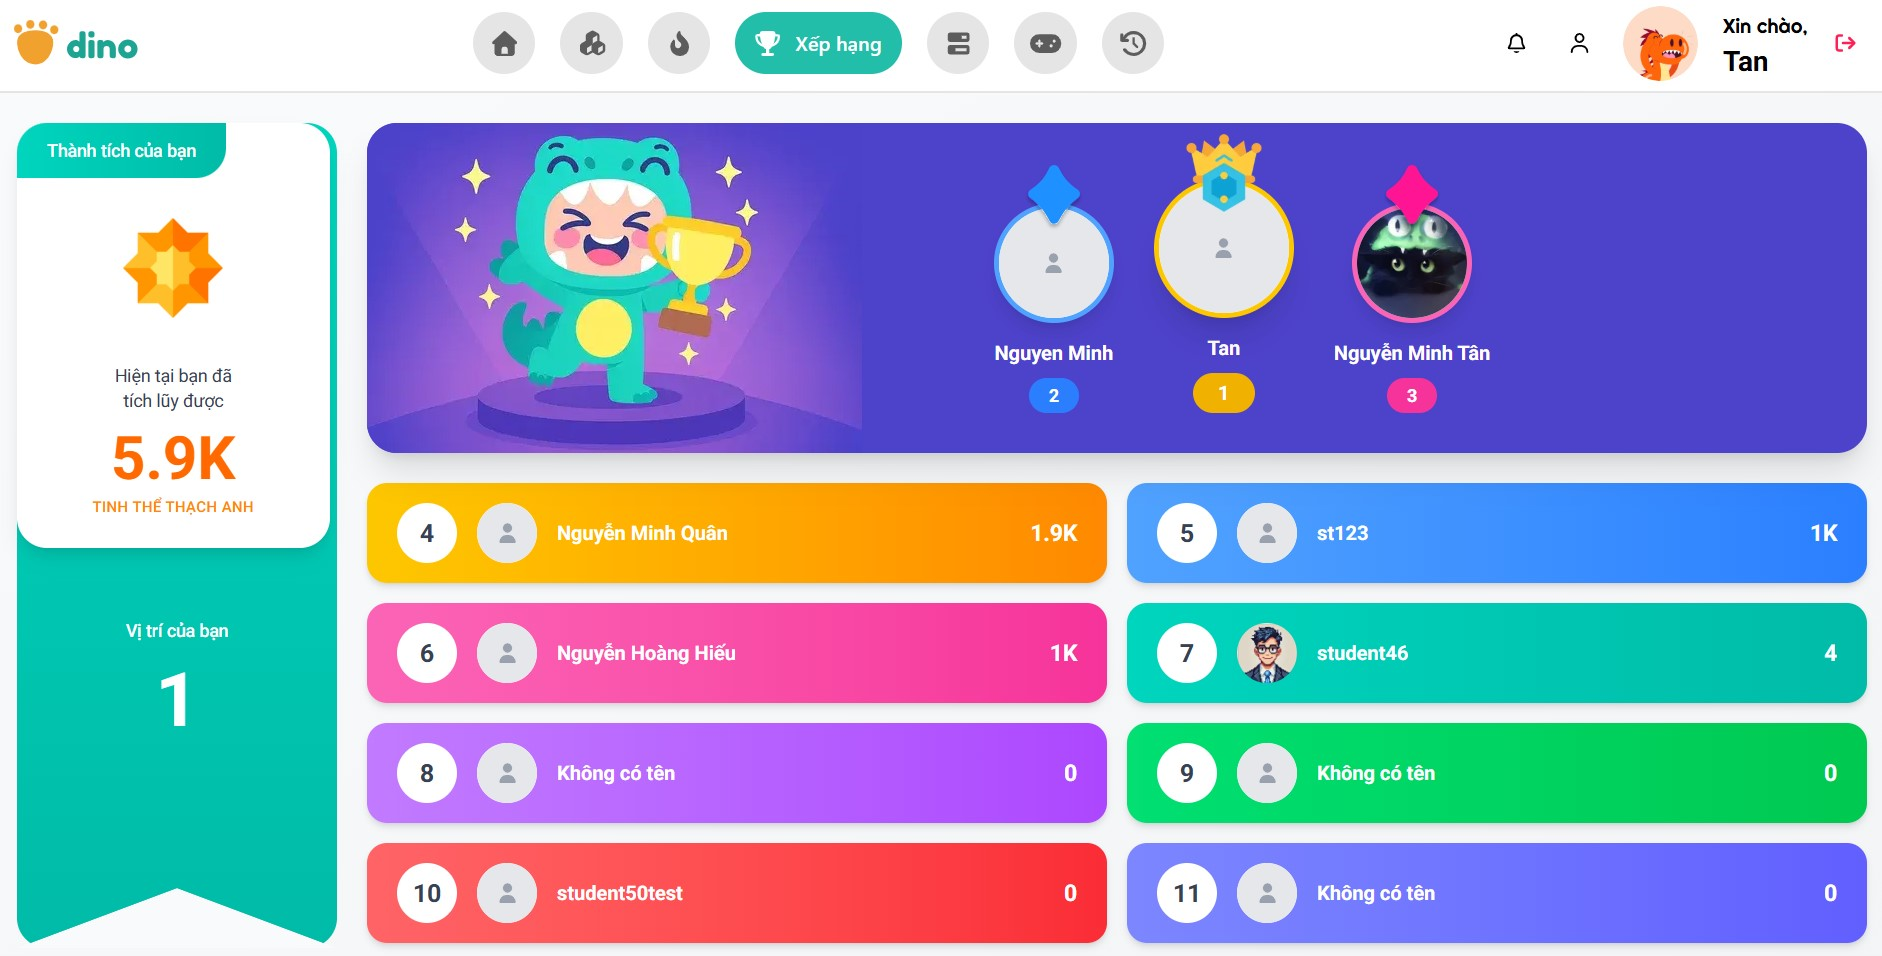
\includegraphics[width=0.9\textwidth]{Image/UI/Main-Student/Leaderboard2.jpg}
		\vspace{0.6cm}
		\caption{Trang Xếp hạng}
	\end{figure}

\subsubsection{Trang Nhiệm vụ}
Trang nhiệm vụ hiển thị các nhiệm vụ hệ thống, phần thưởng là thạch anh. Nếu người dùng hoàn thành được nhiệm vụ đó thì họ có thể nhận phần thưởng tương ứng. Người dùng còn có thể xem các nhiệm vụ đã hoàn thành và các nhiệm vụ chưa hoàn thành.
\begin{figure}[H]
	\centering
	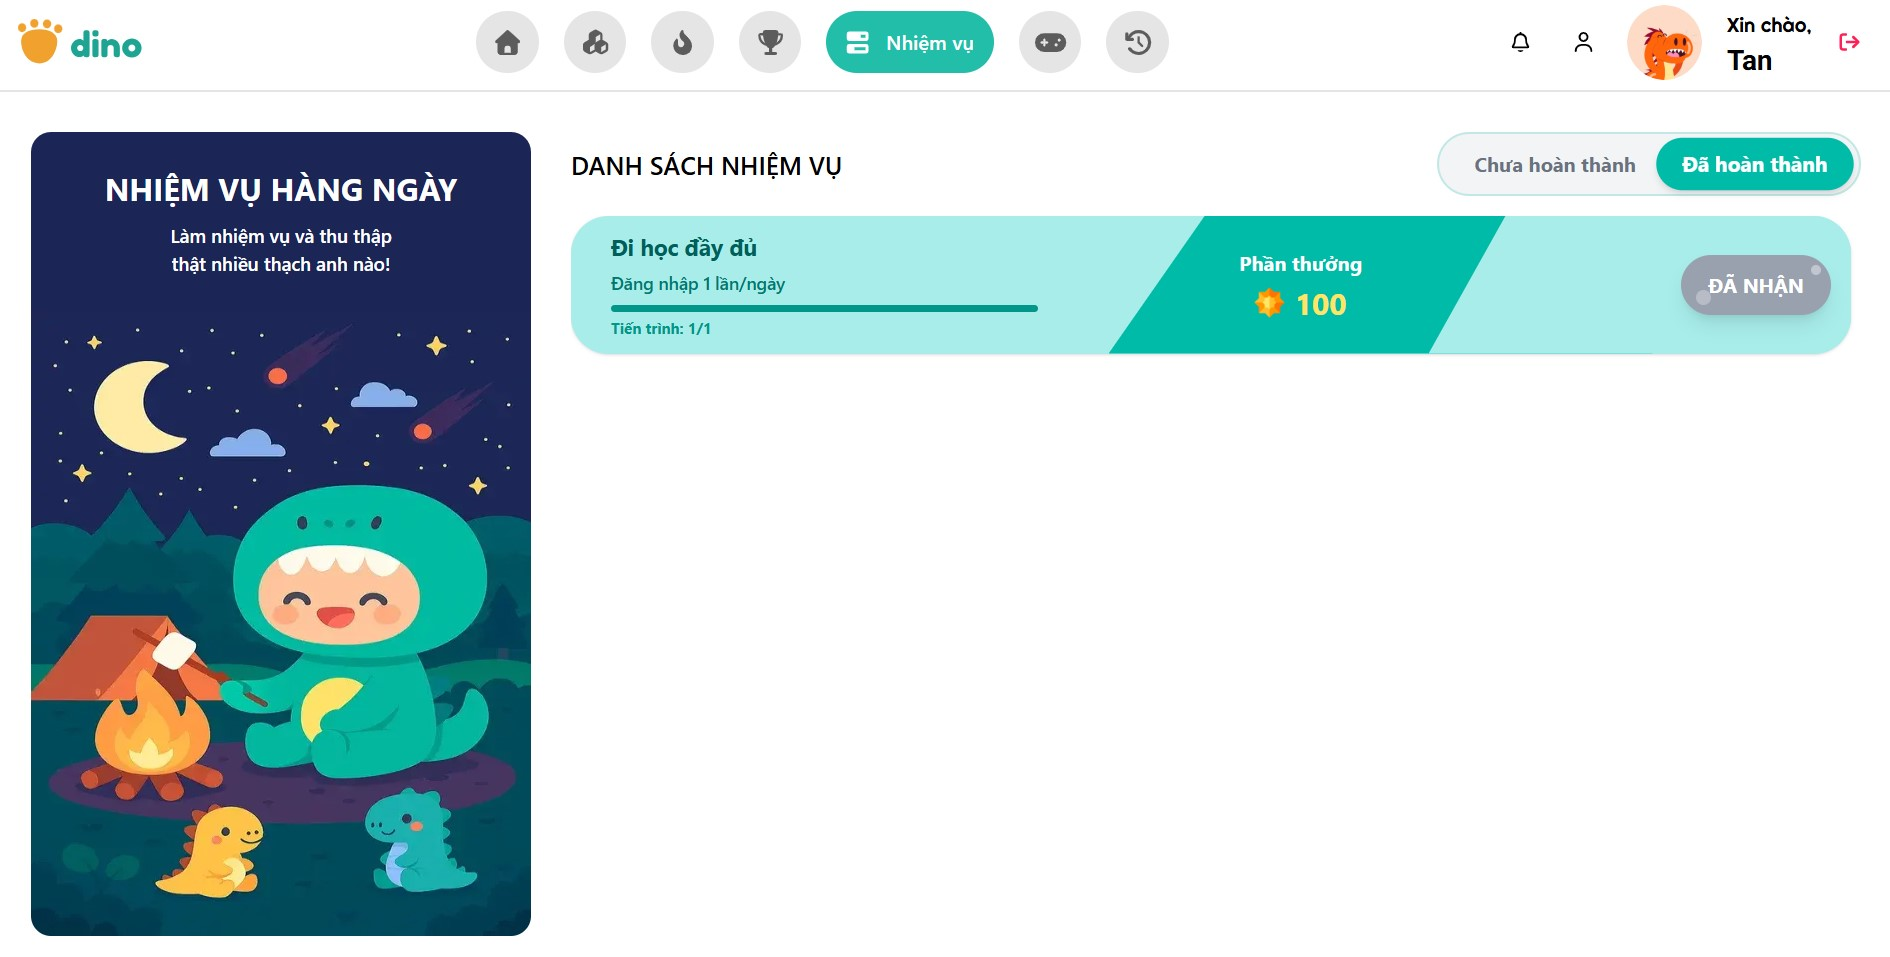
\includegraphics[width=0.9\textwidth]{Image/UI/Main-Student/MissionComplete.jpg}
	\vspace{0.6cm}
	\caption{Trang Nhiệm vụ - Đã hoàn thành}
\end{figure}
\begin{figure}[H]
	\centering
	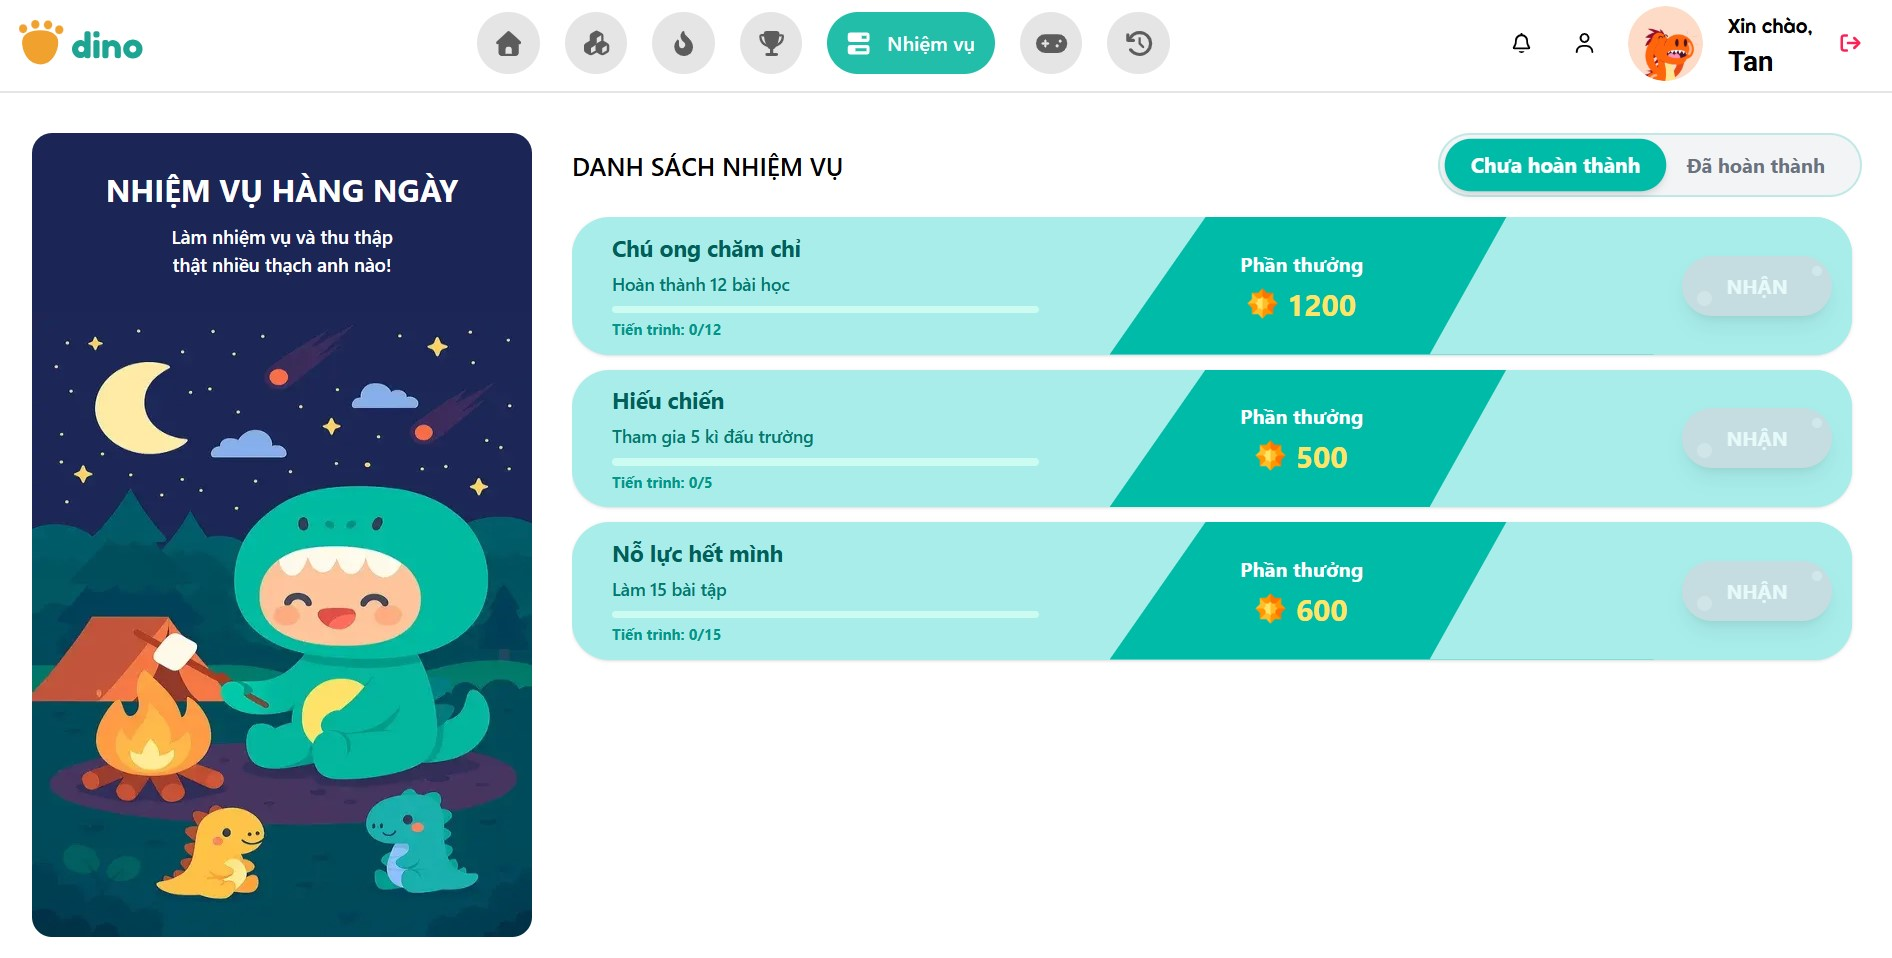
\includegraphics[width=0.9\textwidth]{Image/UI/Main-Student/MissionIncomplete.jpg}
	\vspace{0.6cm}
	\caption{Trang Nhiệm vụ - Chưa hoàn thành}
\end{figure}
\begin{figure}[H]
	\centering
	
\includegraphics[width=0.9\textwidth]{Image/UI/Main-Student/ClaimMission.jpg}
	\vspace{0.6cm}
	\caption{Trang Nhiệm vụ - Nhận thưởng}
\end{figure}

\newpage
\subsubsection{Trang Minigames}
\label{subsubsec:games}
Trang Minigames hiển thị các Minigame bao gồm hai loại chính: Game chơi đơn - nơi người dùng giải quyết các trò chơi toán học cá nhân; và Game tương tác cho phép học sinh đối đầu hoặc hợp tác với phụ huynh và các thành viên khác trong Family để cùng giải toán. Tại đây, người dùng có thể tham gia trò chơi ngay lập tức bằng cách bấm vào nút \textit{Chơi ngay}, sau đó, một tab mới trên trình duyệt sẽ được mở và giao diện trò chơi được hiển thị, ví dụ như \textit{Hình \ref{fig:mathmatch}}.
\begin{figure}[H]
	\centering
	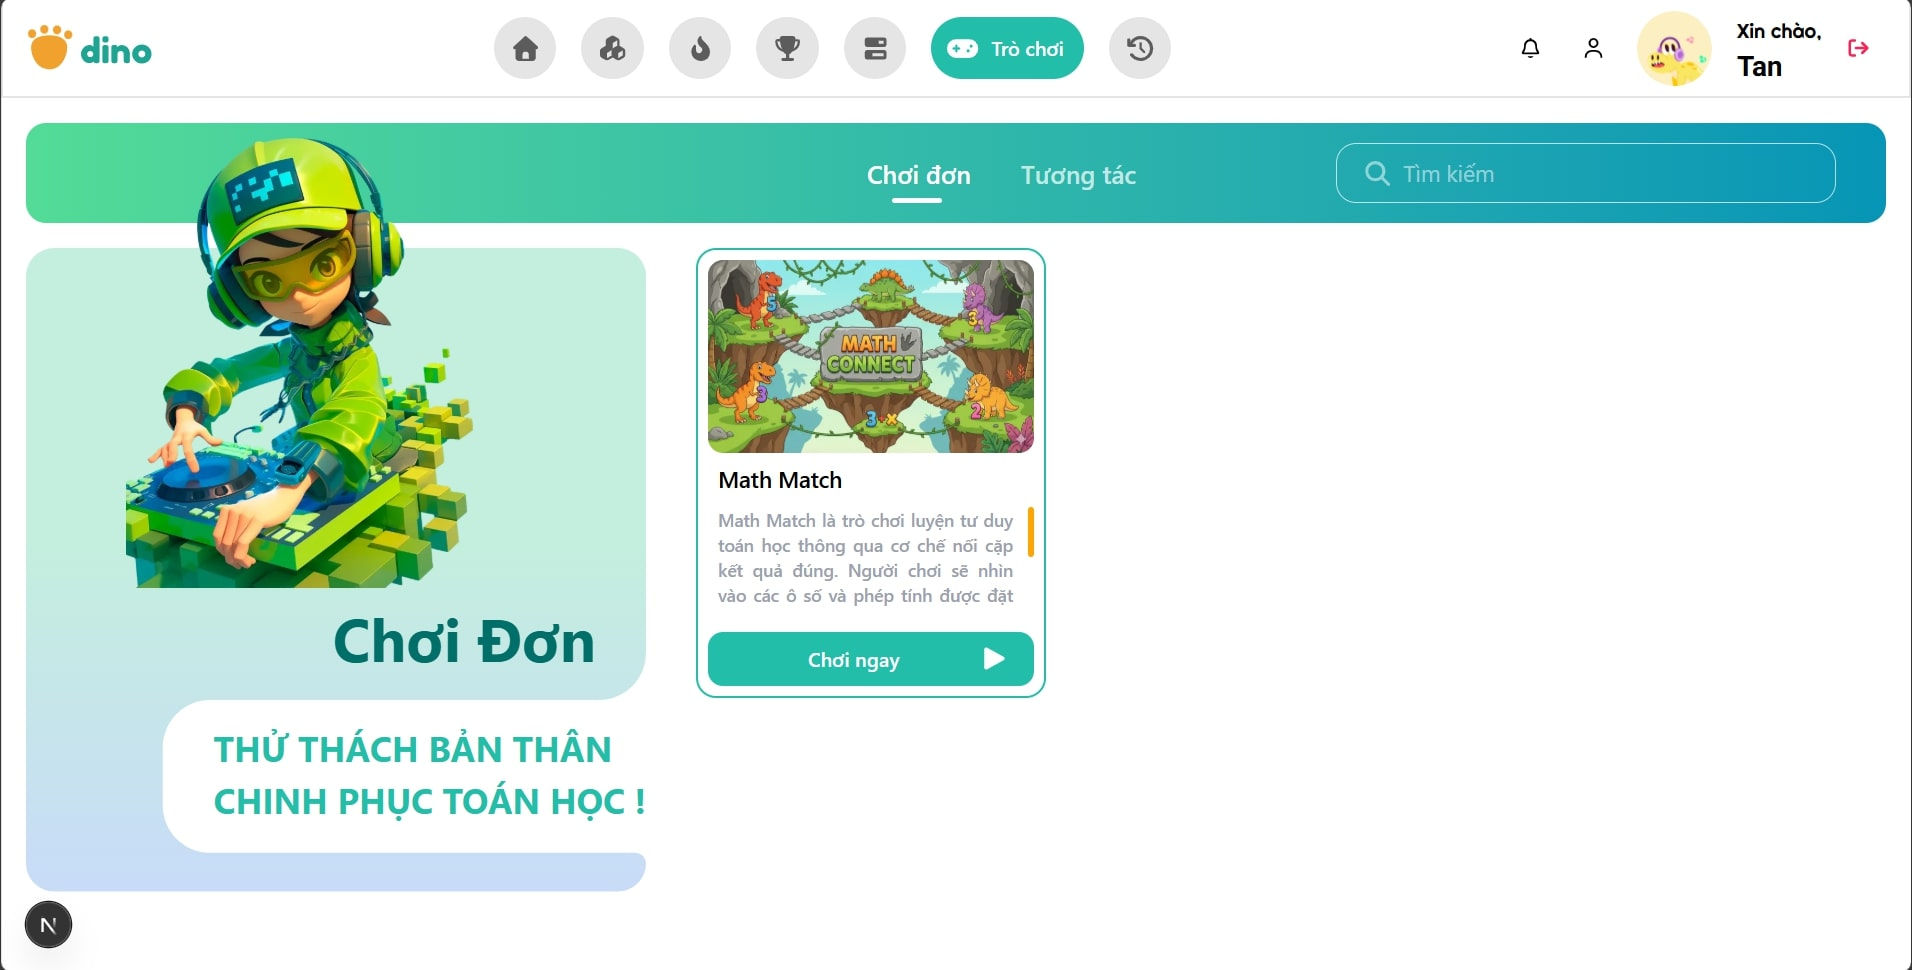
\includegraphics[width=0.9\textwidth]{Image/UI/Main-Student/Game-Single.jpg}
	\vspace{0.6cm}
	\caption{Trang Minigame - Chơi đơn}
\end{figure}
\begin{figure}[H]
	\centering
	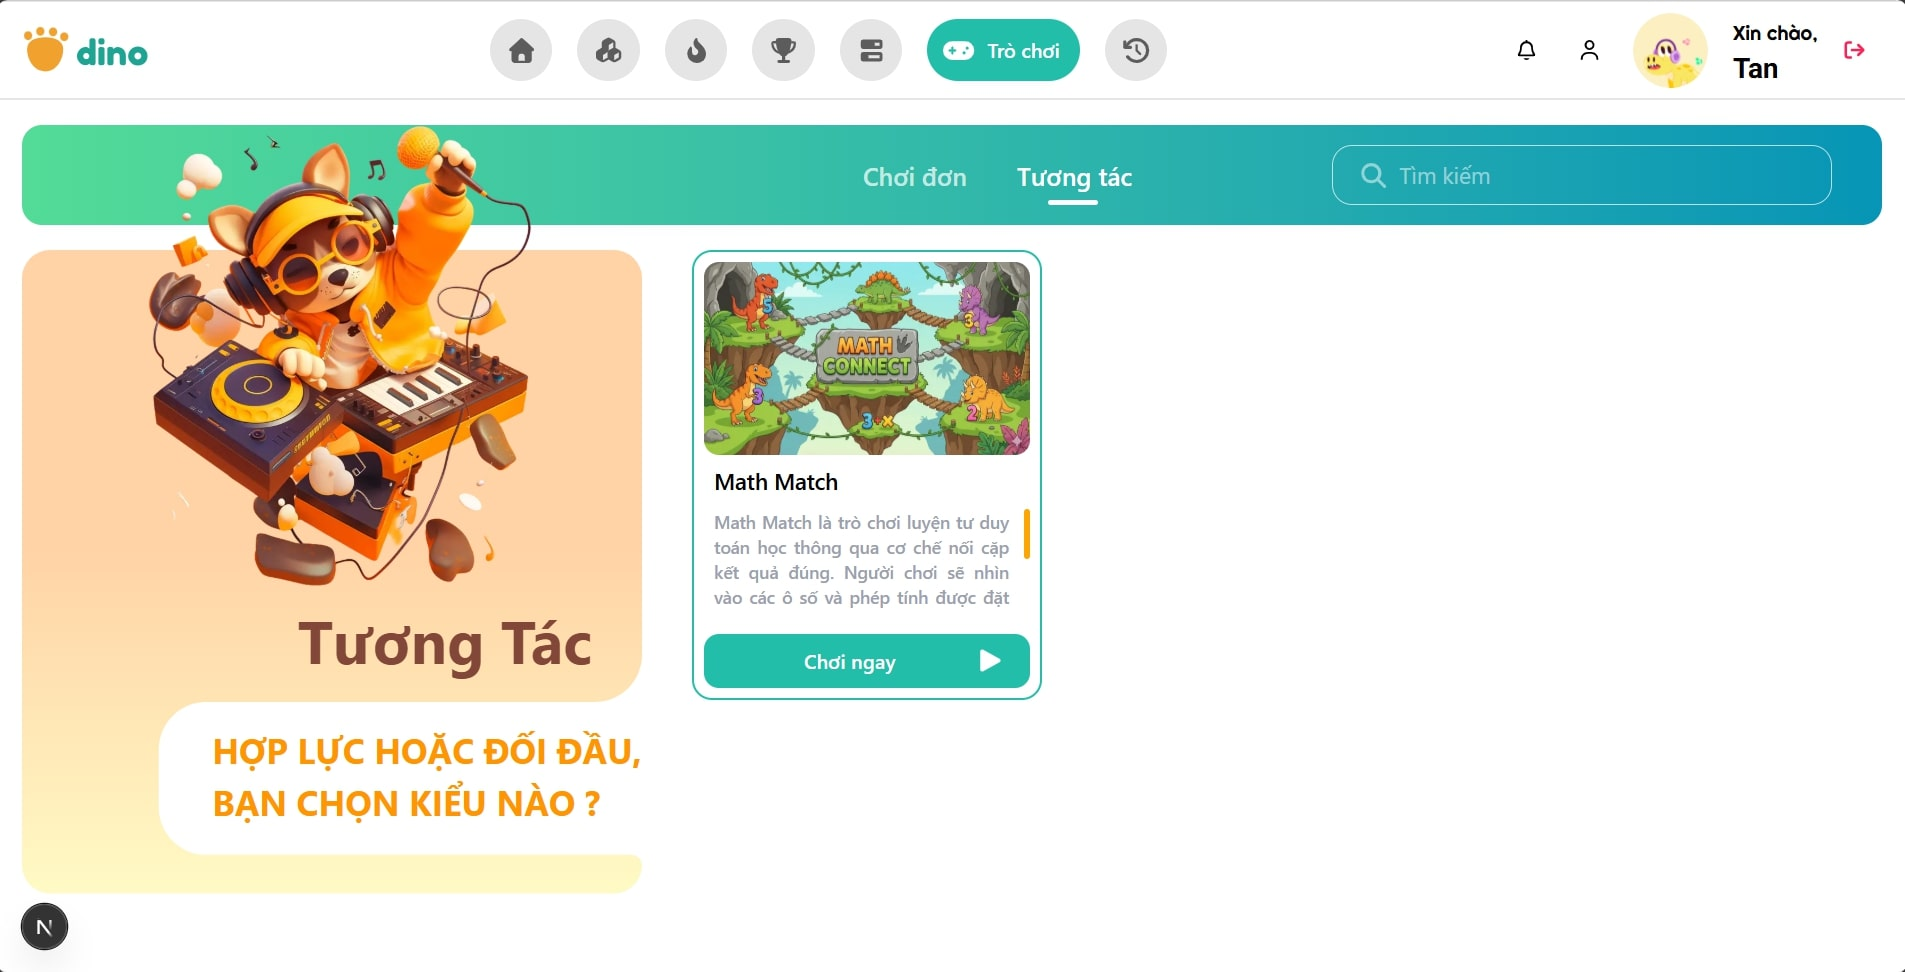
\includegraphics[width=0.9\textwidth]{Image/UI/Main-Student/Game-PVP.jpg}
	\vspace{0.6cm}
	\caption{Trang Minigame - Tương tác}
\end{figure}

\newpage
Minigame chơi đơn có tên gọi \textbf{Math Match}. Đây là trò chơi mang lối chơi tương tự như game Pikachu cổ điển, nơi người chơi cần tìm và nối các cặp ô phù hợp để loại bỏ chúng khỏi màn hình. Tuy nhiên, thay vì nối các hình giống nhau, người chơi trong Math Match phải nối các phép tính có \textbf{kết quả bằng nhau}. Điều này không chỉ tạo sự quen thuộc về cơ chế chơi mà còn tăng thêm yếu tố tư duy và tính toán.

Trong quá trình chơi, người chơi cần quan sát nhanh, tính toán chính xác và lựa chọn đường nối hợp lệ giữa các ô để hoàn thành màn chơi trong thời gian giới hạn. Để tăng tính hấp dẫn và hỗ trợ người chơi trong những tình huống khó, game còn được tích hợp thêm các \textbf{item bổ trợ}. Ví dụ, item dạng “rocket” có thể giúp phá hủy một số ô bất kỳ trên màn hình, tạo ra khoảng trống thuận lợi cho việc nối các cặp còn lại. Bên cạnh đó, item “hint” sẽ gợi ý các cặp ô có thể nối được, giúp người chơi tiếp tục khi không tìm thấy nước đi

Sự kết hợp giữa yếu tố giải đố, tính toán và các cơ chế hỗ trợ đã giúp Math Match trở nên thú vị hơn, vừa mang tính giải trí vừa góp phần rèn luyện khả năng tư duy logic và phản xạ của người chơi.
\begin{figure}[H]
	\centering
	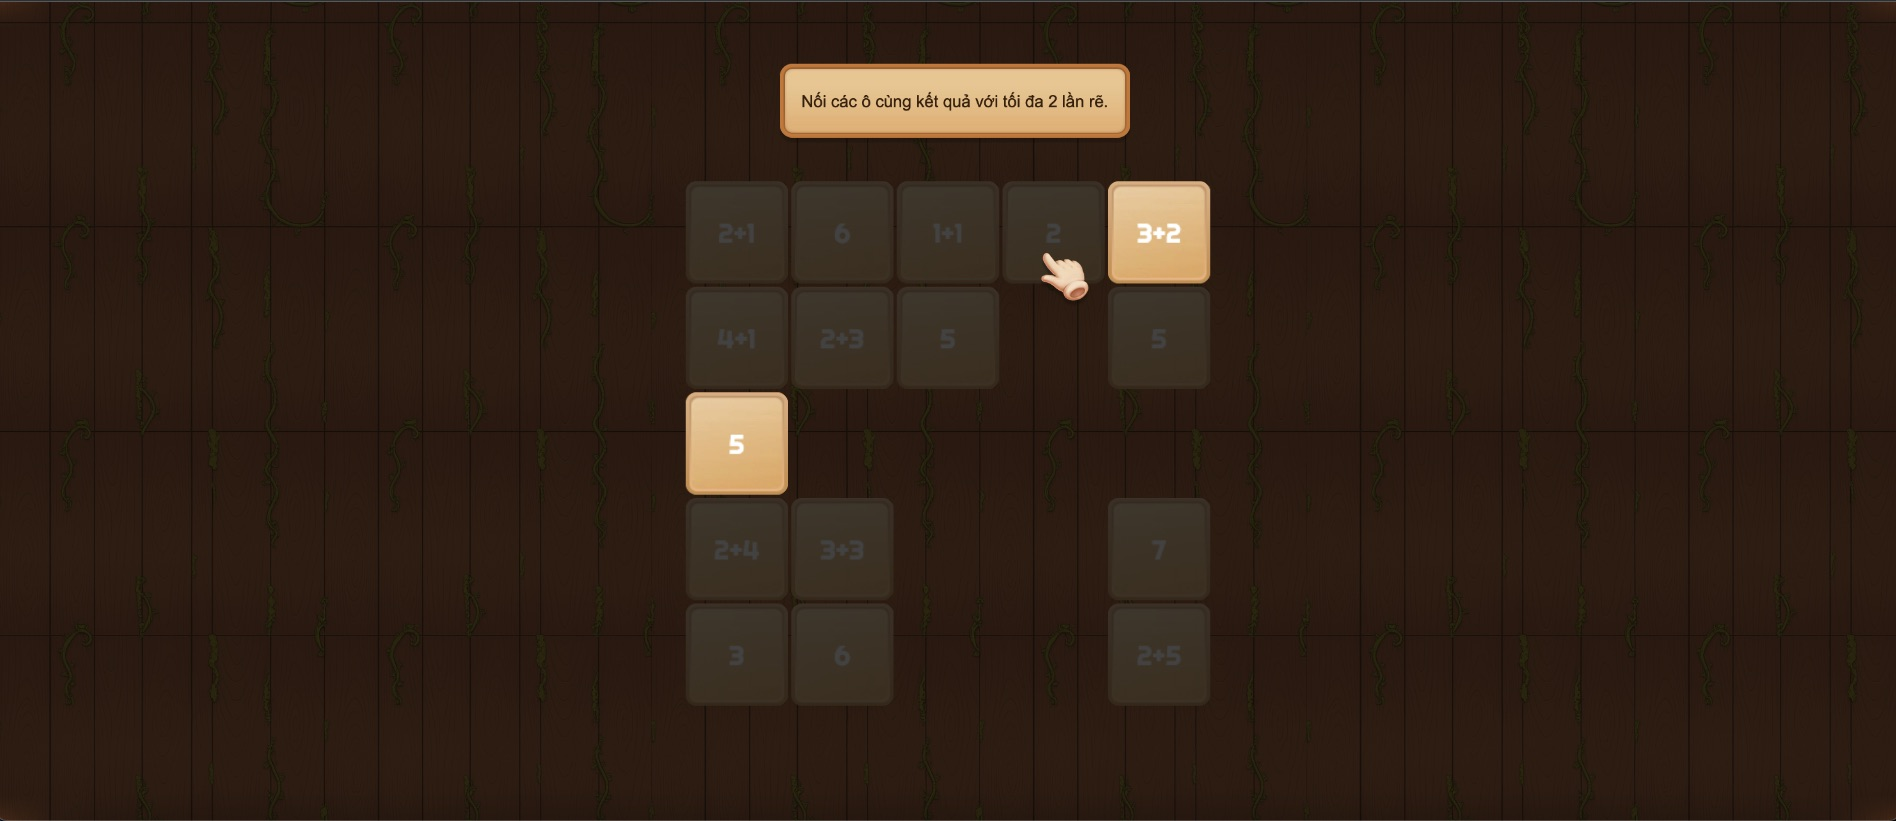
\includegraphics[width=0.9\textwidth]{Image/UI/Main-Student/MathMatchGame.jpeg}
	\vspace{0.6cm}
	\caption{Trang Minigame - Minigame Math Match}
	\label{fig:mathmatch}
\end{figure}

\newpage
 Minigame tương tác 2 người với tên gọi \textbf{Tomato Shooting}. Game được lấy ý tưởng từ tựa game Gunny, trong đó hai người chơi đối đầu trực tiếp với nhau theo thời gian thực thông qua máy chủ đa người chơi \textbf{Colyseus} tích hợp trong Cocos Creator. Mỗi màn chơi bao gồm 5 vòng, mỗi vòng hệ thống sẽ hiển thị một phép tính toán học, người chơi phải bắn quả cà chua tới quả bóng mang kết quả đúng trước đối thủ để giành chiến thắng trong vòng đó. Sau 5 vòng, người chơi nào thắng nhiều vòng hơn sẽ là người chiến thắng chung cuộc. Cơ chế thời gian thực và yếu tố cạnh tranh trực tiếp giúp tăng tính hấp dẫn, đồng thời vẫn đảm bảo mục tiêu luyện tập tính toán nhanh cho học sinh.
\begin{figure}[H]
	\centering
	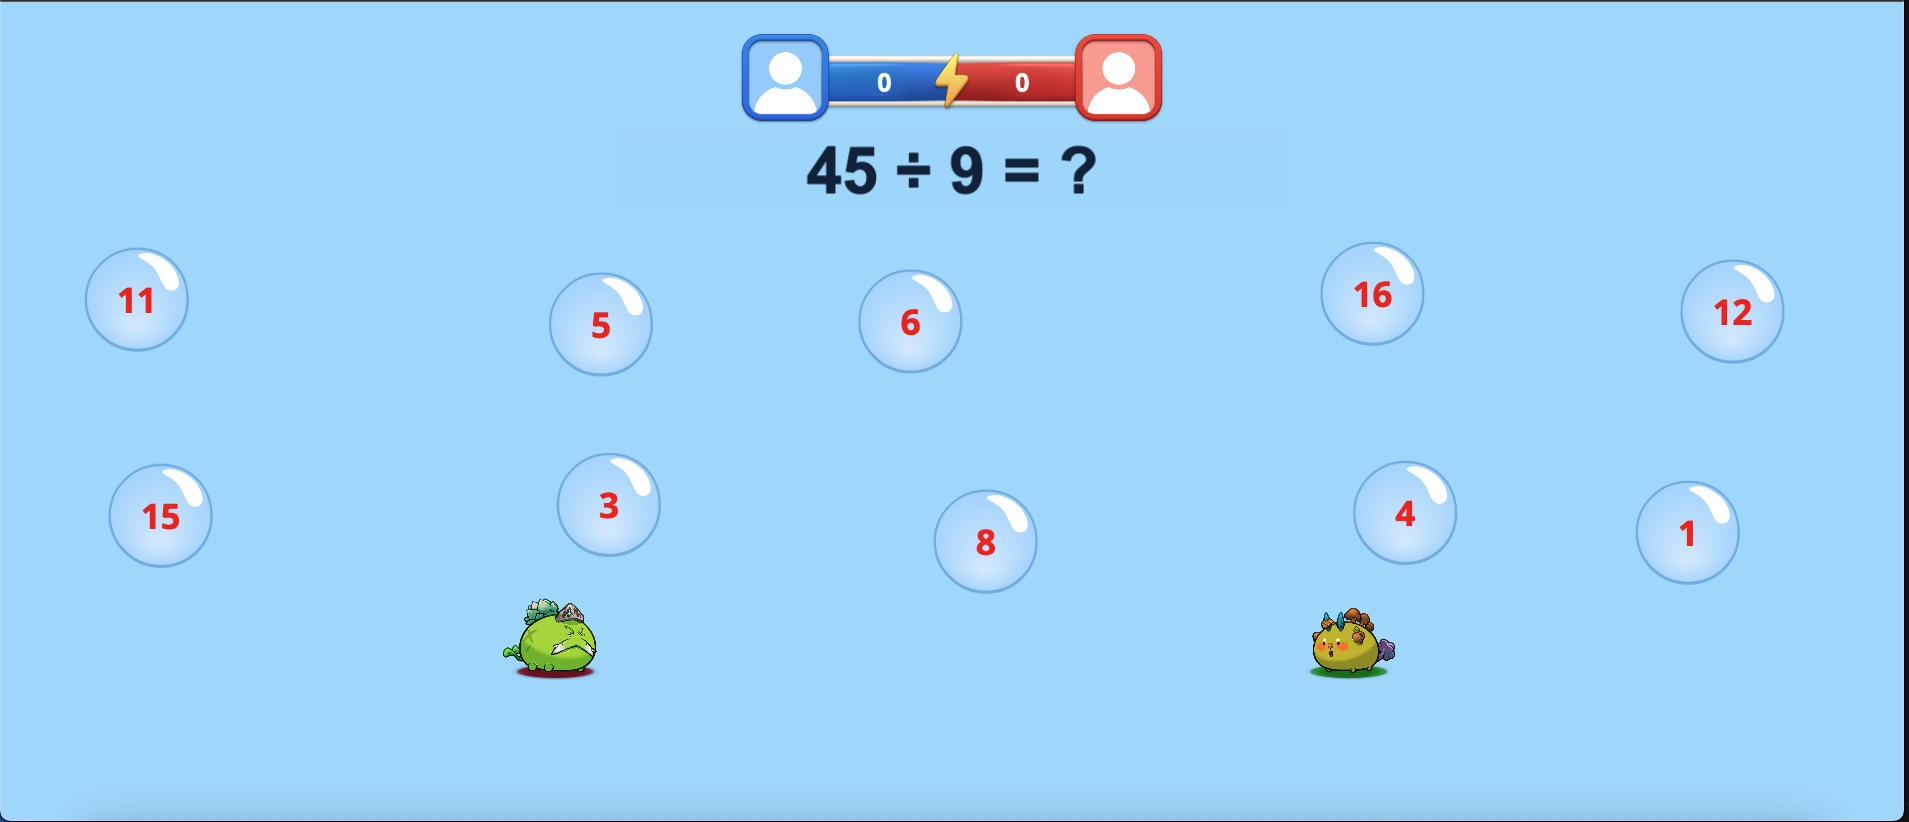
\includegraphics[width=0.9\textwidth]{Image/UI/Main-Student/TomatoesShootingGame.jpeg}
	\vspace{0.6cm}
	\caption{Trang Minigame - Minigame Tomato Shooting}
	\label{fig:tomatoshooting}
\end{figure}

\subsubsection{Trang Lịch sử làm bài}
Người dùng có thể dễ dàng theo dõi tiến độ thông qua việc lọc lịch sử làm bài và xem các chỉ số thống kê về số lượng, độ chính xác trung bình của bài tập. Giao diện chính của trang lịch sử làm bài được thiết kế như hình bên dưới.
\begin{figure}[H]
	\centering
	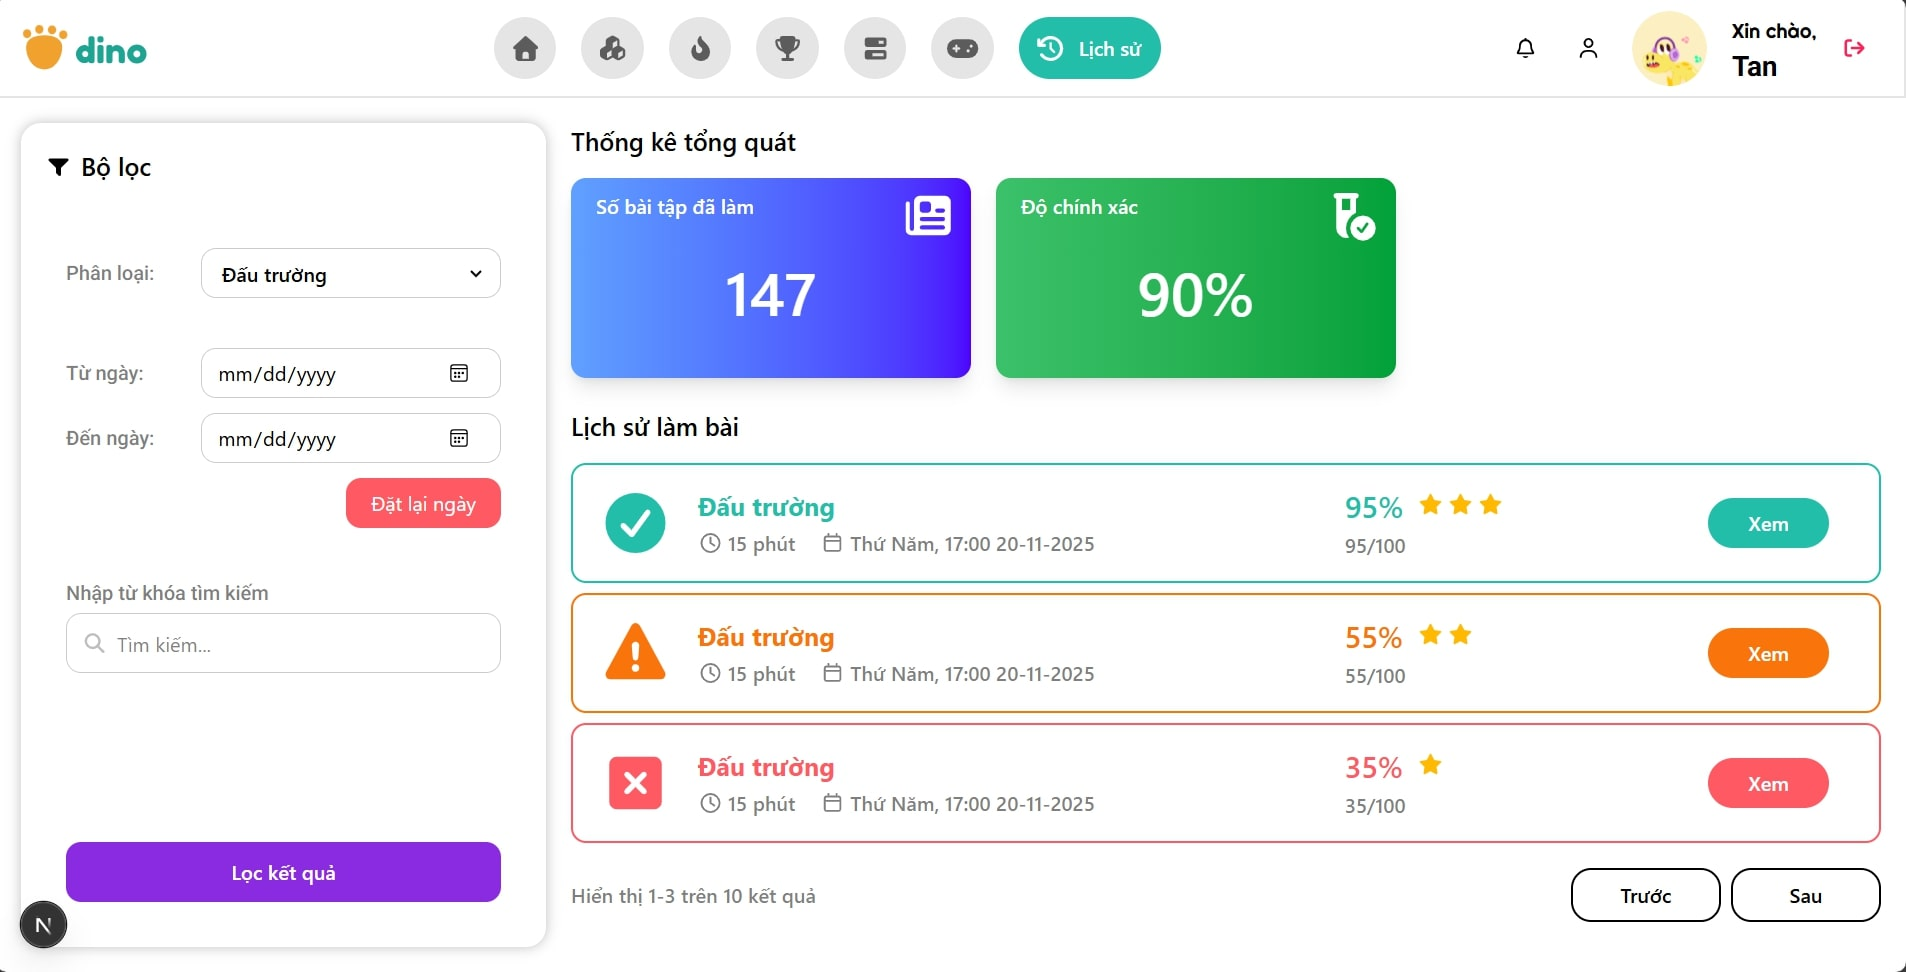
\includegraphics[width=0.9\textwidth]{Image/UI/Main-Student/History.jpg}
	\vspace{0.6cm}
	\caption{Trang Lịch sử làm bài}
	\label{fig:history}
\end{figure}

\newpage
Khi bấm vào nút \textit{Xem} trên các bản ghi được hiển thị ở  \textit{Hình \ref{fig:history}}, người dùng còn có thể xem chi tiết bài làm với các thông tin như: thời gian làm bài, thời gian hoàn thành, tổng số câu, số câu đúng, số câu sai. Đặc biệt, người dùng có thể biết mình làm sai hoặc đúng câu nào cũng như đáp án chính xác của câu đó. Giao diện chi tiết bài làm được thiết kế như 2 hình dưới đây.
\begin{figure}[H]
	\centering
	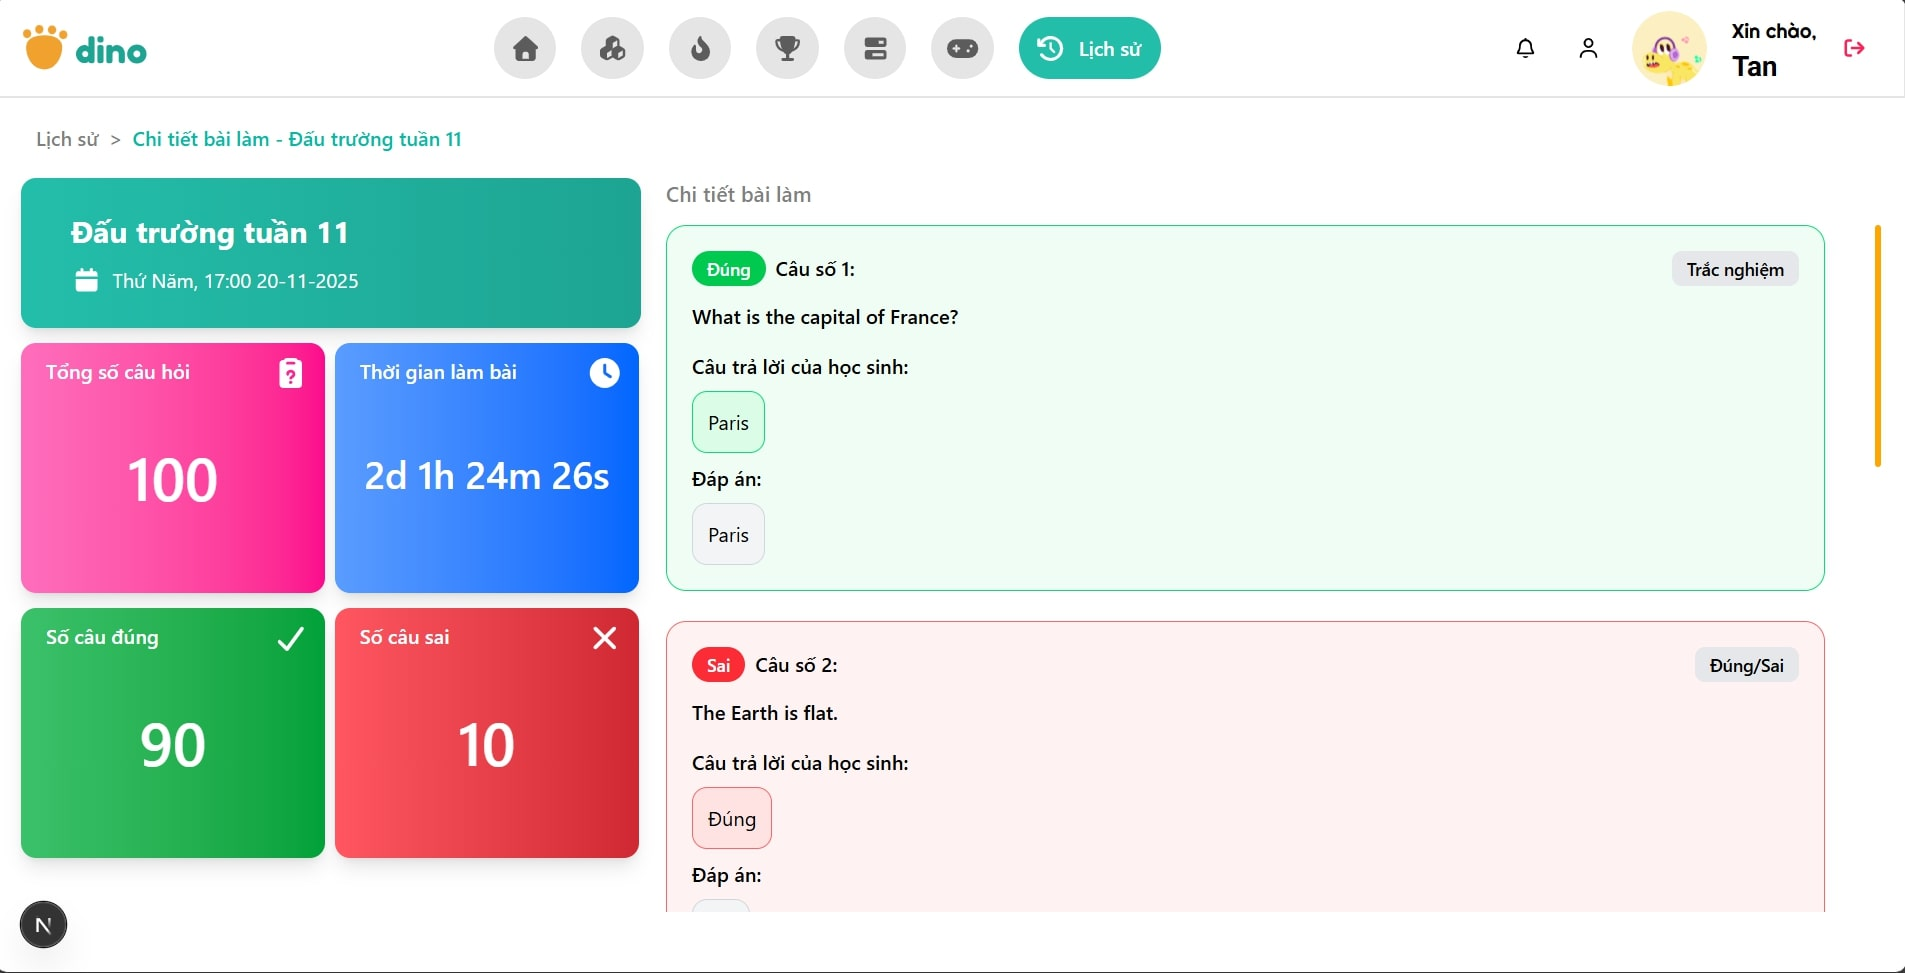
\includegraphics[width=0.9\textwidth]{Image/UI/Main-Student/ExamDetail1.jpg}
	\vspace{0.6cm}
	\caption{Trang Lịch sử làm bài - Chi tiết bài làm}
\end{figure}
\begin{figure}[H]
	\centering
	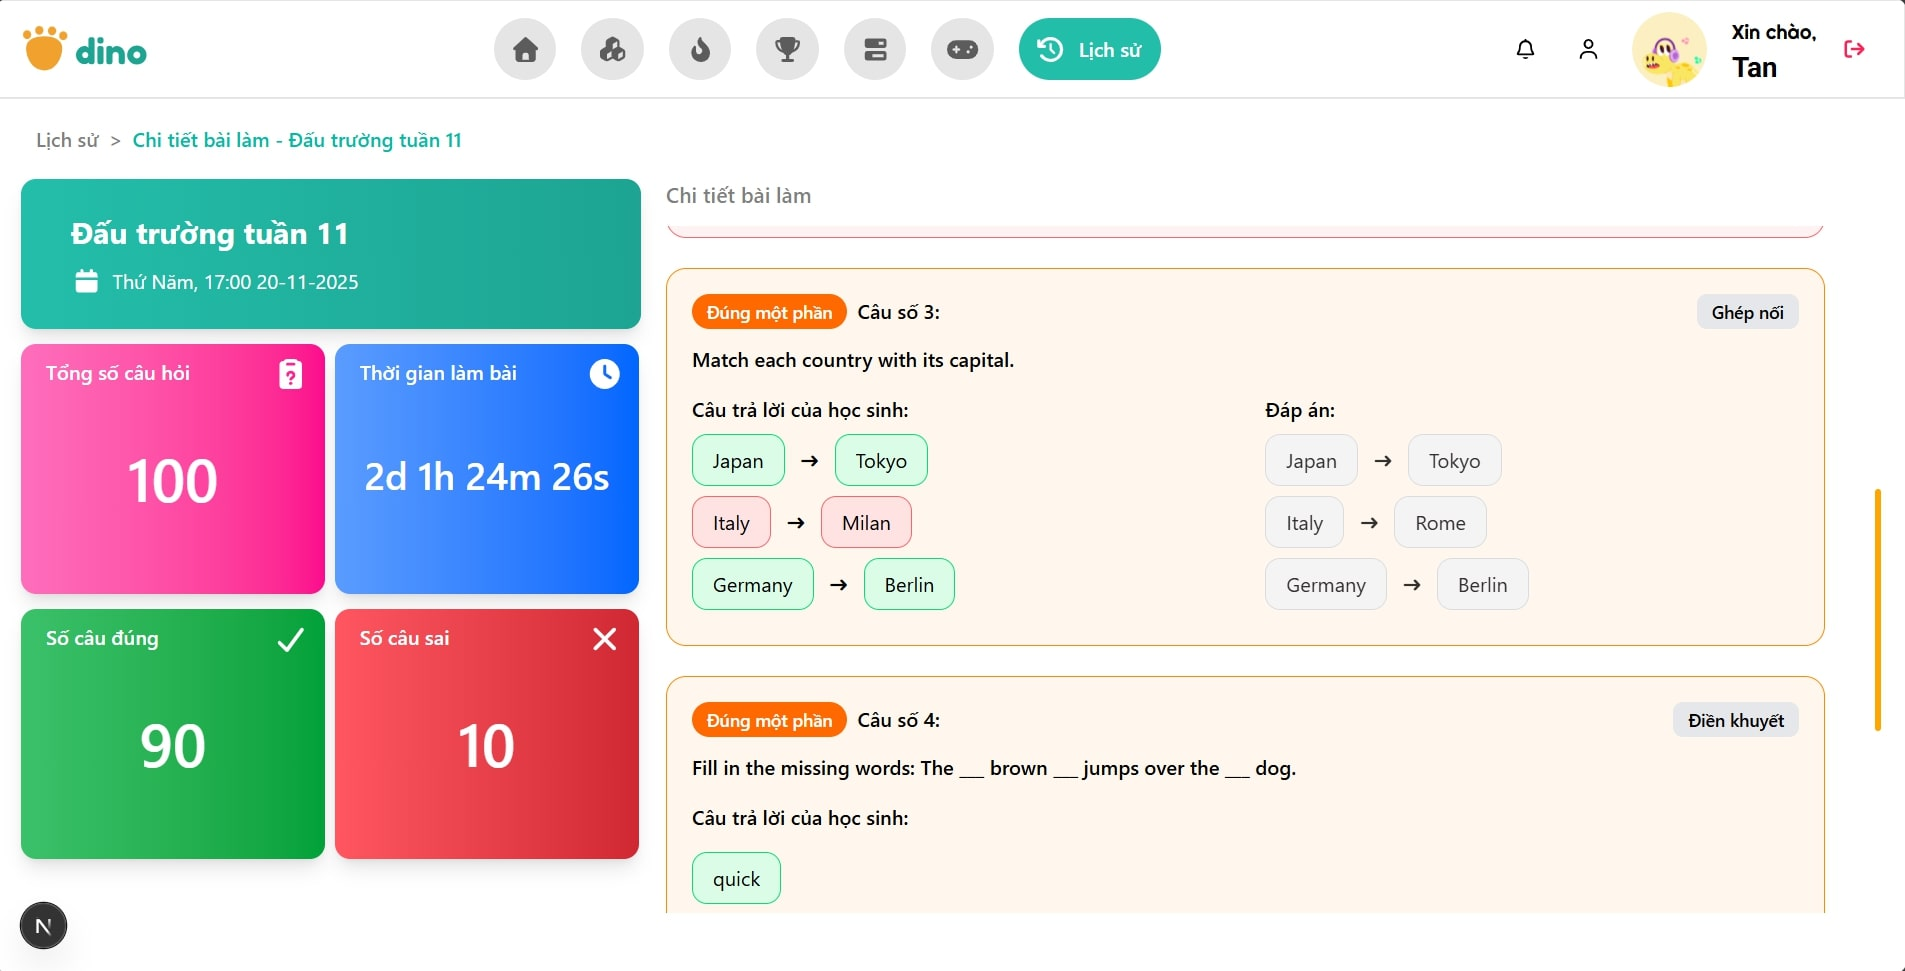
\includegraphics[width=0.9\textwidth]{Image/UI/Main-Student/ExamDetail2.jpg}
	\vspace{0.6cm}
	\caption{Trang Lịch sử làm bài - Chi tiết bài làm}
\end{figure}

\newpage
\subsubsection{Quản lý tài khoản cá nhân}
\label{subsubsec:profile}
\begin{enumerate}
\item \textbf{Xem và cập nhật thông tin cá nhân}
\vspace{0.1cm}
\newline
	Học sinh có thể xem và chỉnh sửa thông tin cá nhân, bao gồm ảnh đại diện, họ và tên, khối lớp. Tuy nhiên, email là cố định với mỗi tài khoản và chỉ được quyền xem.
	\begin{figure}[H]
		\centering
		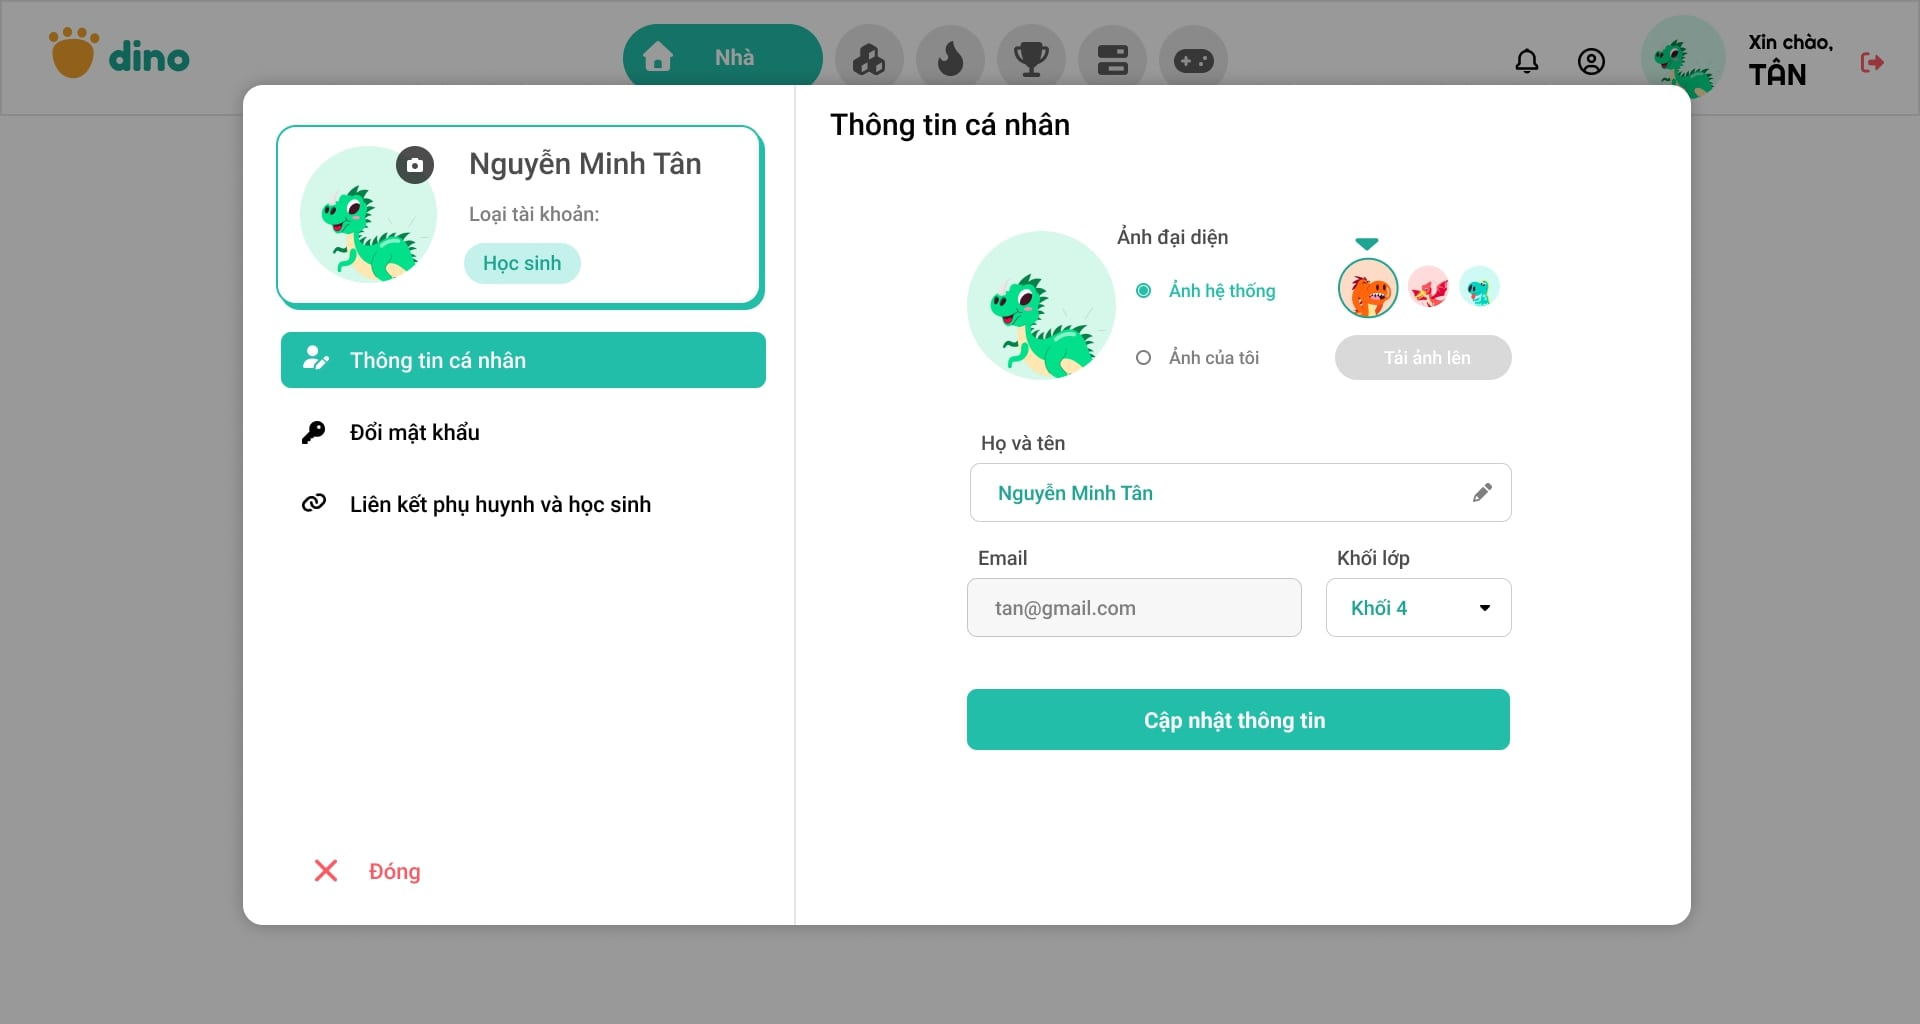
\includegraphics[width=0.9\textwidth]{Image/UI/Main-Student/Info.jpg}
		\vspace{0.6cm}
		\caption{Quản lý tài khoản cá nhân - Xem và cập nhật thông tin}
	\end{figure}

\item \textbf{Thay đổi mật khẩu}
\vspace{0.1cm}
\newline	
Học sinh có thể thay đổi mật khẩu bằng cách nhập các thông tin như mật khẩu hiện tại, mật khẩu mới và xác nhận mật khẩu. Chỉ có thể thay đổi mật khẩu khi các thông tin trên thỏa mãn các điều kiện sau:
		\begin{itemize}
			\item Giá trị của tất cả các field khác rỗng.
			\item Giá trị của field mật khẩu hiện tại phải trùng khớp.
			\item Mật khẩu có ít nhất 8 ký tự, trong đó phải chứa chữ cái in hoa, chữ thường, số và ký tự đặc biệt.
			\item Mật khẩu và Xác nhận mật khẩu phải trùng khớp. 
		\end{itemize}

		\begin{figure}[H]
			\centering
			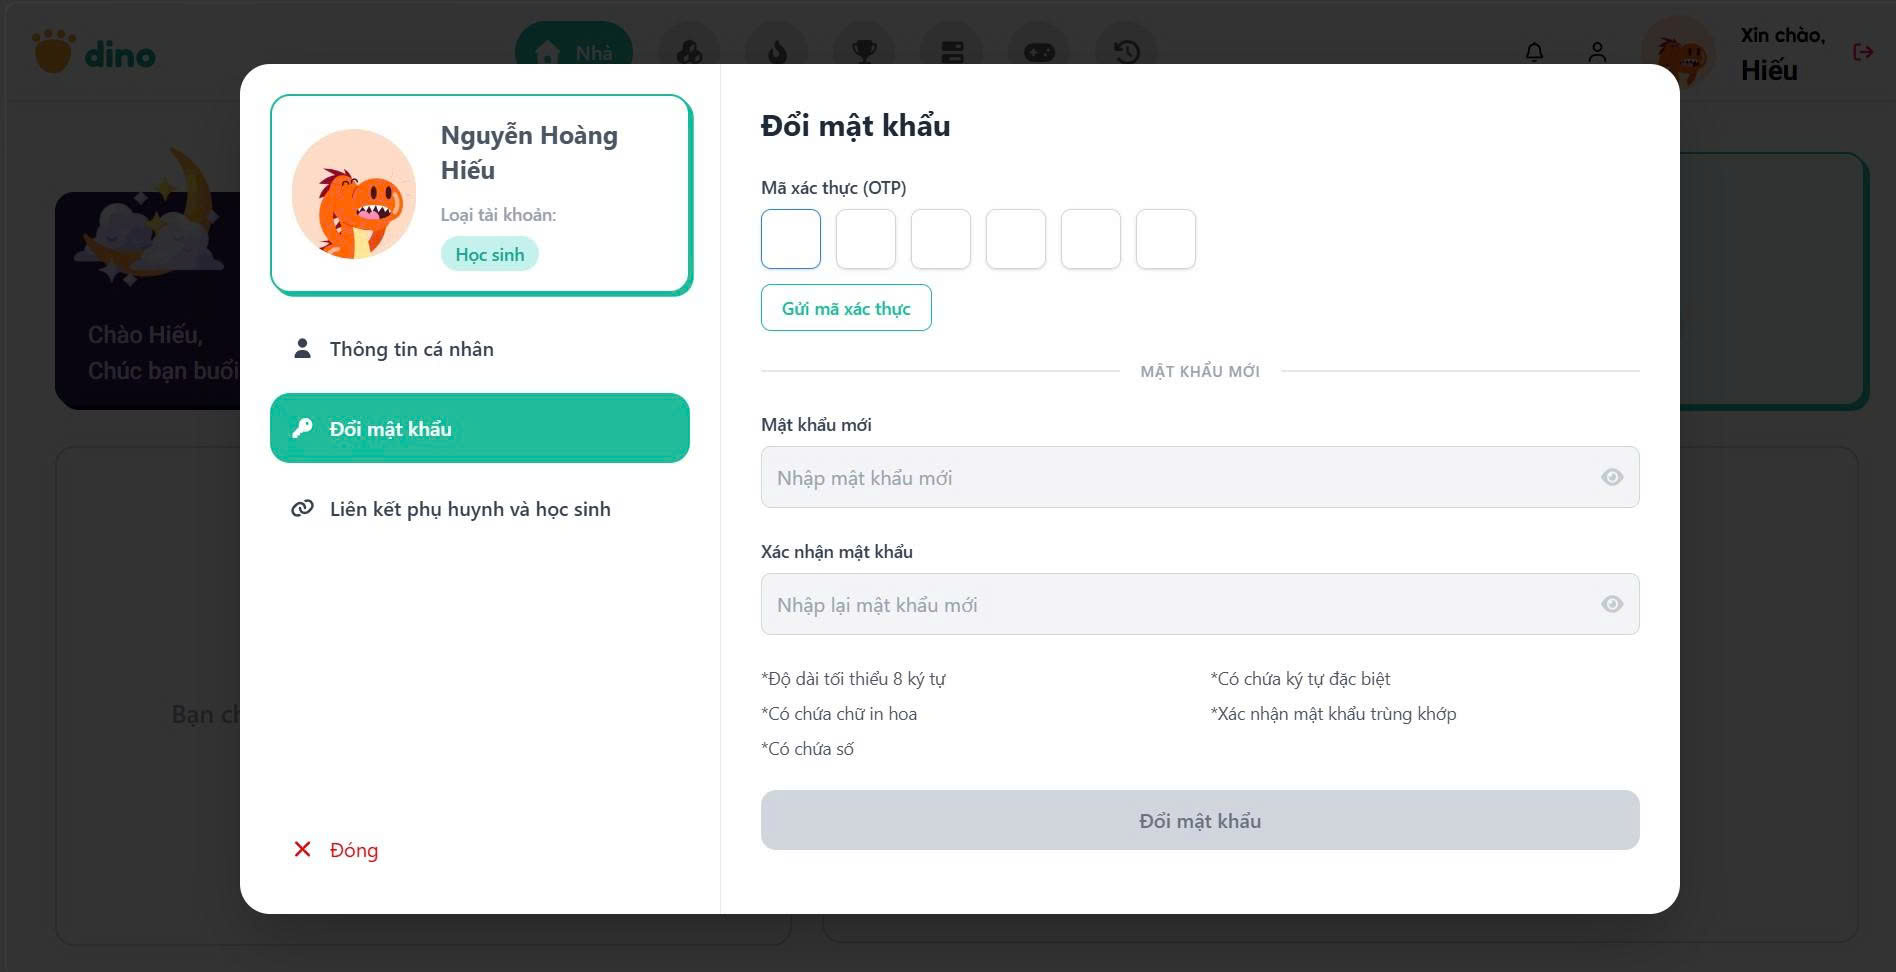
\includegraphics[width=0.9\textwidth]{Image/UI/Main-Student/ChangePassword.jpg}
			\vspace{0.6cm}
			\caption{Quản lý tài khoản cá nhân - Thay đổi mật khẩu}
		\end{figure}

	
\item \textbf{Liên kết tài khoản}
\vspace{0.1cm}
\newline
Tại giao diện này, học sinh có thể xem mã liên kết (mã mời) của Family hiện tại và có thể chia sẻ cho các học sinh khác. Ngoài ra, học sinh còn có thể xem đươc phụ huynh nào đang quản lý Family của mình.
		\begin{figure}[H]
			\centering
			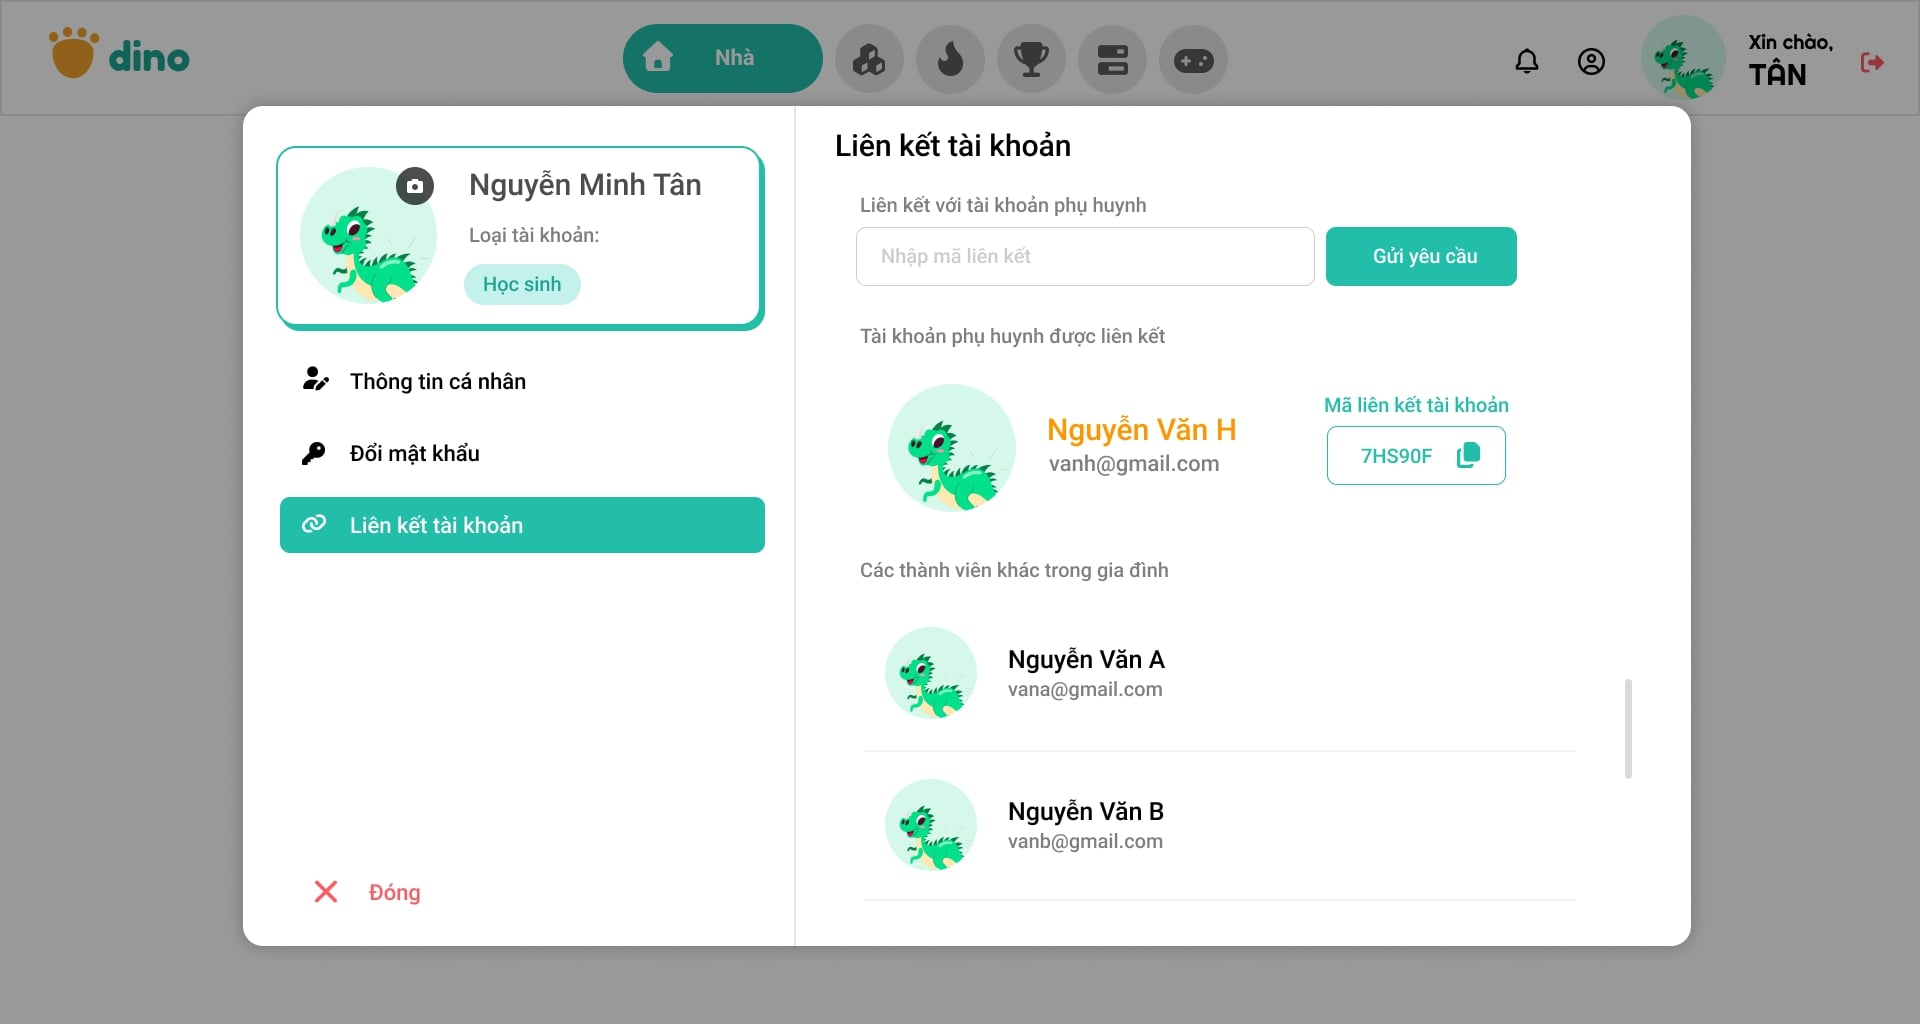
\includegraphics[width=0.9\textwidth]{Image/UI/Main-Student/Account-Linked.jpg}
			\vspace{0.6cm}
			\caption{Quản lý tài khoản cá nhân - Đã liên kết tài khoản}
		\end{figure}
\end{enumerate}

\subsection{Các màn hình chính của tài khoản Phụ huynh}
\subsubsection{Trang Thống kê tổng quan}
\label{subsubsec:parenthome}
Mỗi phụ huynh sẽ là quản trị viên của một Family và có thể quản lý nhiều học sinh khác nhau. Vì thế, ở phần bộ lọc bên trái, ngoài lọc theo thời gian còn có lọc theo học sinh. Ở phần nội dung giữa màn hình, phụ huynh có thể xem các thống kê tổng quan về học tập và đấu trường của học sinh được chọn.
	\begin{figure}[H]
		\centering
		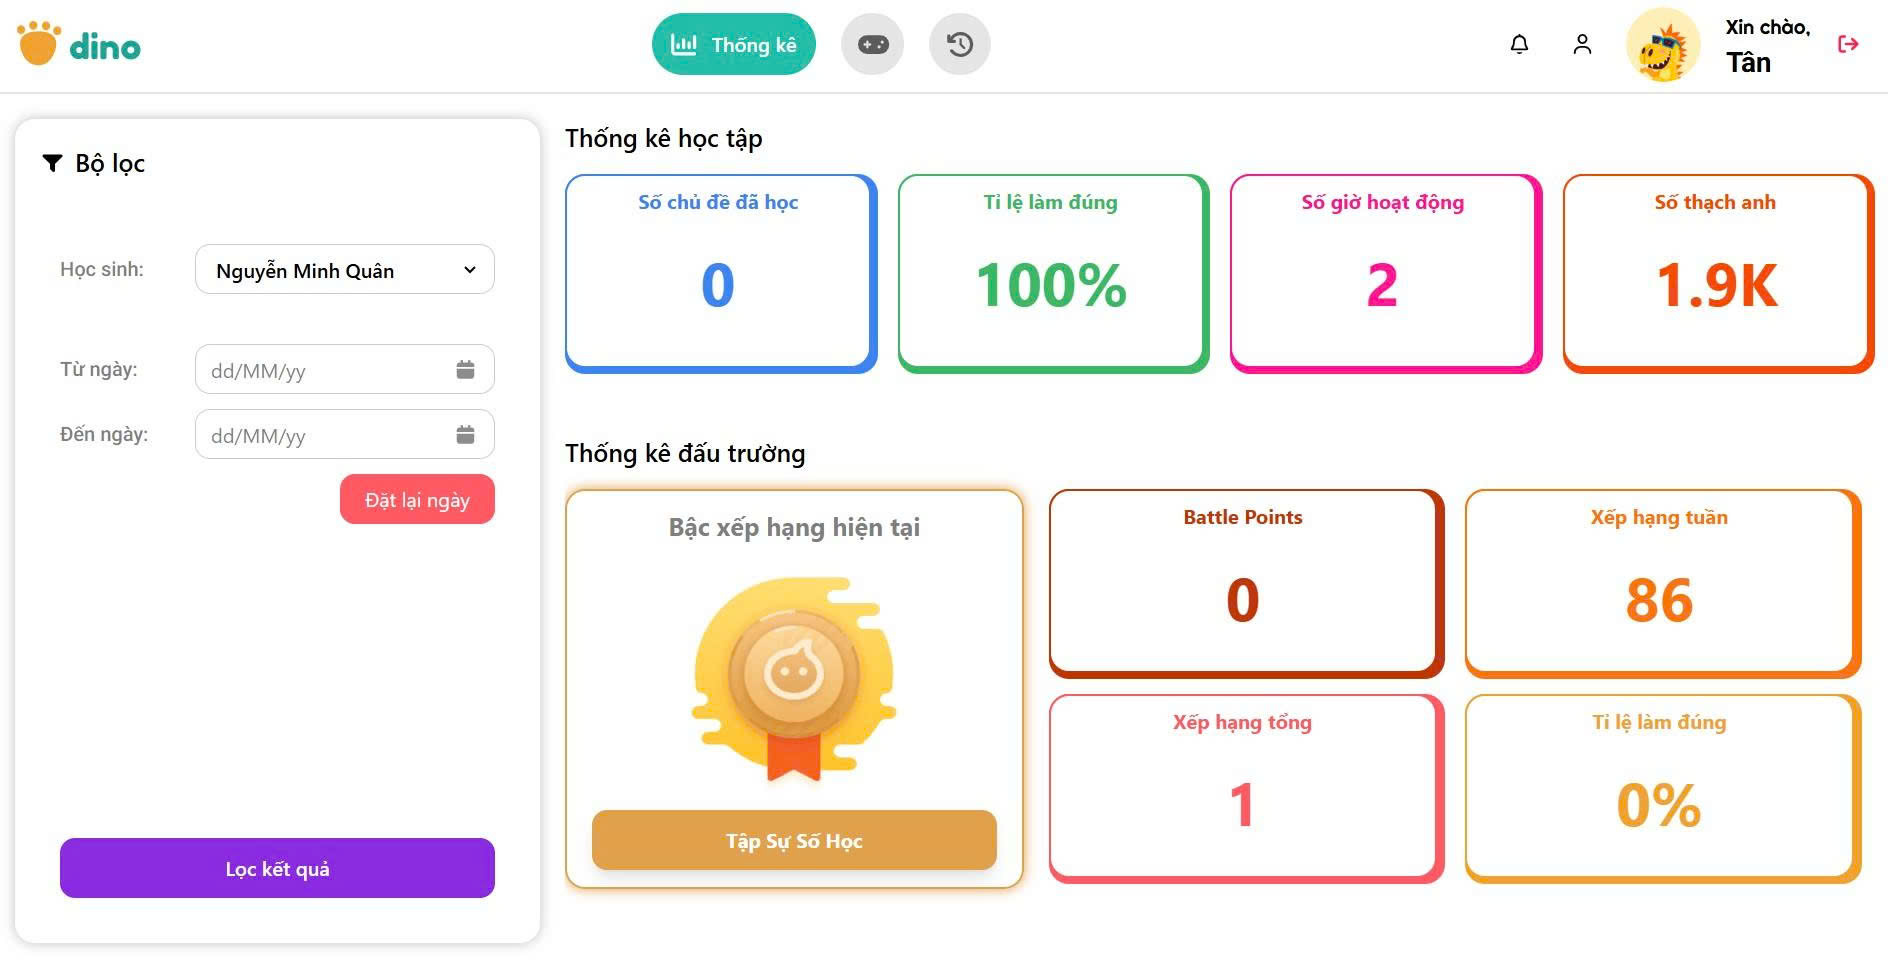
\includegraphics[width=0.9\textwidth]{Image/UI/Main-Parent/Statistics.jpg}
		\vspace{0.6cm}
		\caption{Thống kê tổng quan}
	\end{figure}


\subsubsection{Trang Lịch sử bài làm}
Phụ huynh có thể xem lịch sử các lần làm bài của học sinh, xem thống kê tổng quan về số bài tập đã làm và tỉ lệ làm đúng trung bình. Phụ huynh có thể thay đổi bộ lọc ở bên trái để dễ dàng lọc các bản ghi. Trên mỗi bản ghi có hiển thị thông tin về tên bài tập, thời gian làm bài, thời gian kết thúc, số câu đúng và đánh giá mức độ bằng số sao và màu sắc. Giao diện lịch sử làm bài của phụ huynh được thiết kế như hình bên dưới.
\begin{figure}[H]
 	\centering
 	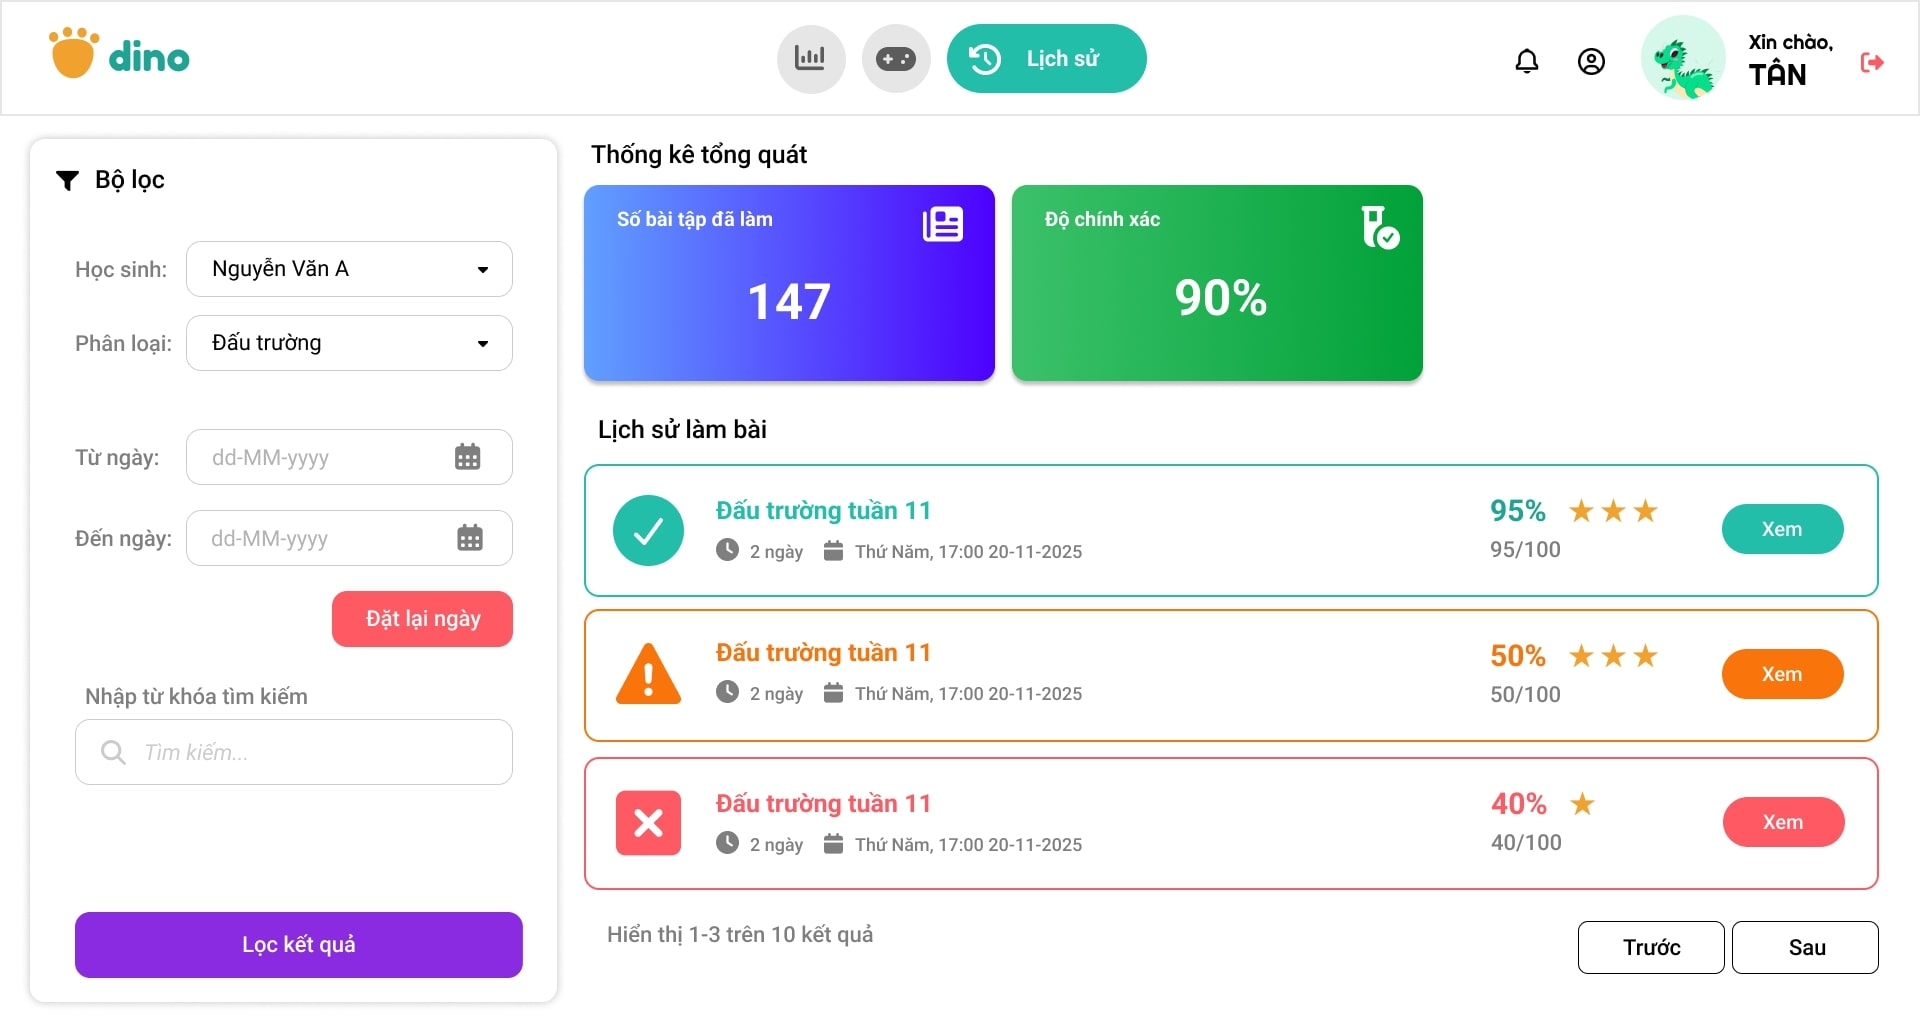
\includegraphics[width=0.9\textwidth]{Image/UI/Main-Parent/History.jpg}
 	\vspace{0.6cm}
 	\caption{Lịch sử làm bài}
 \end{figure}
 
\vspace{0.2cm}
\newline
Phụ huynh còn có thể xem chi tiết bài làm của học sinh bằng cách bấm vào nút \textit{Xem} trên mỗi bản ghi. Trang chi tiết bài làm bao gồm thông tin tổng quan của bài làm (tên học sinh, lớp, thời gian hoàn thành, thời gian làm bài, tổng số câu, số câu đúng/sai). Ngoài ra, phụ huynh có thể đánh giá năng lực của con thông qua chi tiết các câu trả lời. Giao diện chi tiết bài làm được thiết kế như hình dưới đây.
	\begin{figure}[H]
		\centering
		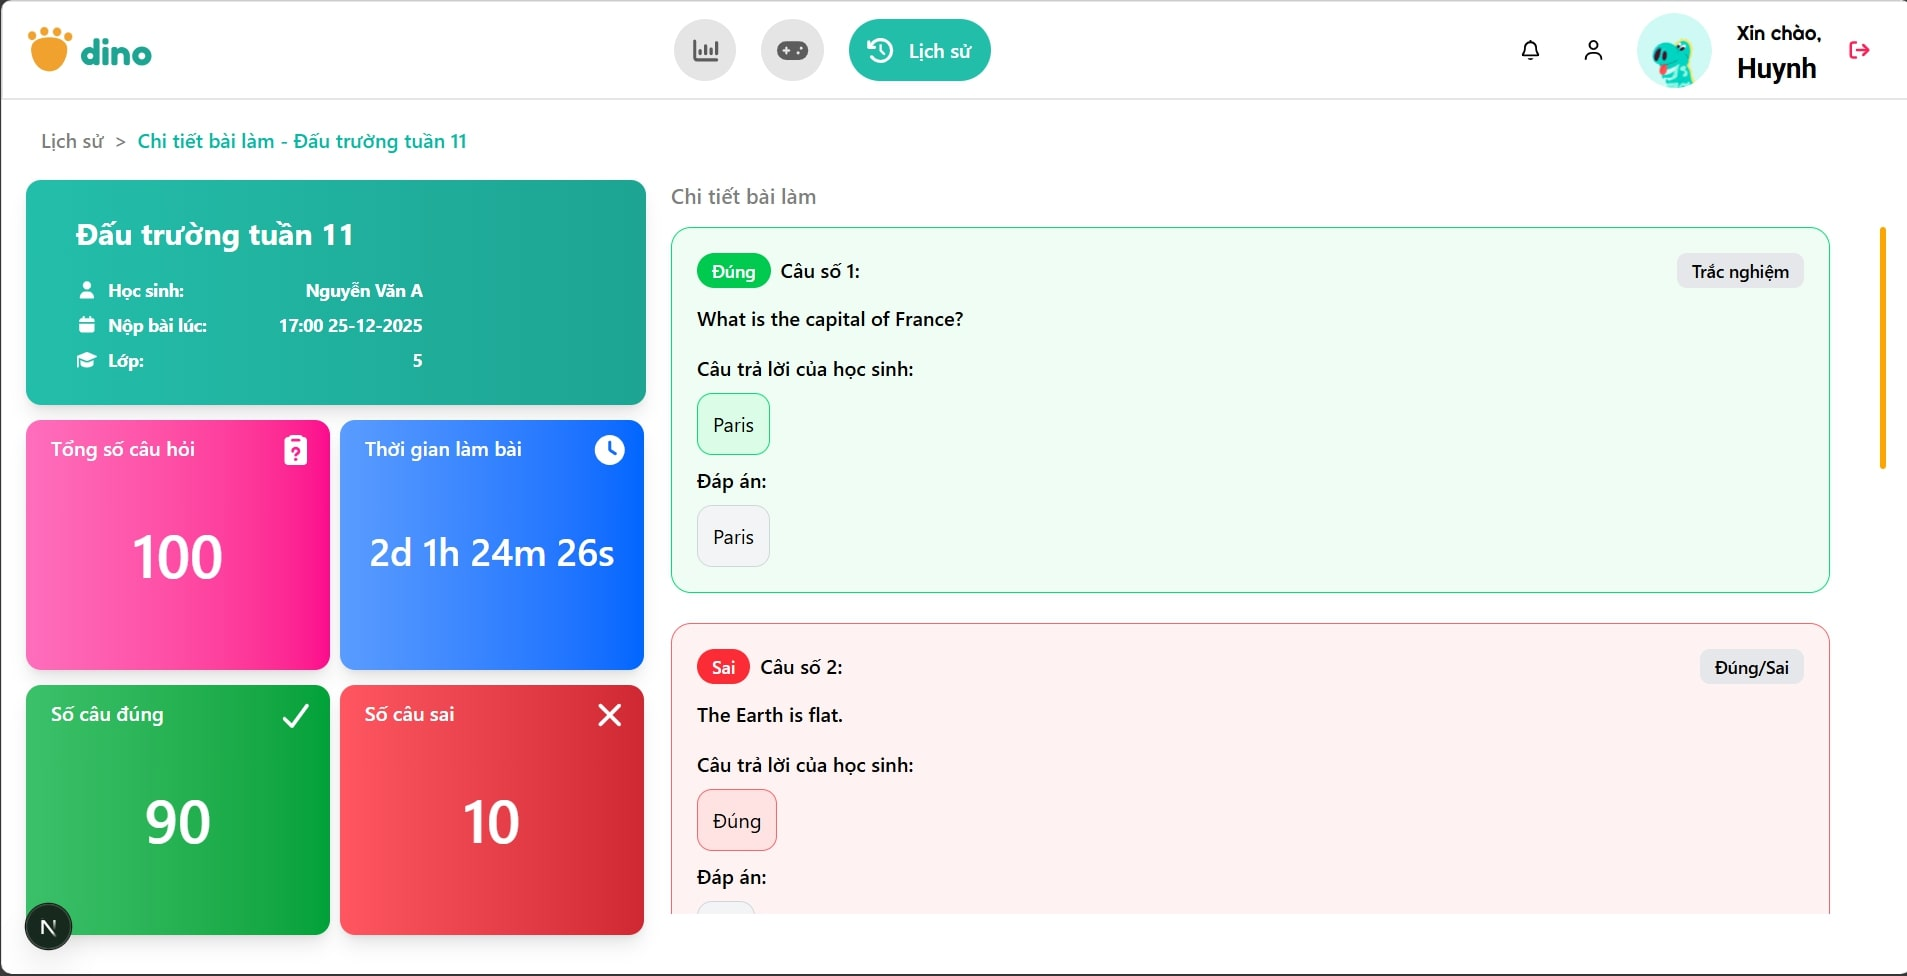
\includegraphics[width=0.9\textwidth]{Image/UI/Main-Parent/ExamDetail.jpg}
		\vspace{0.6cm}
		\caption{Chi tiết bài làm}
	\end{figure}

\subsubsection{Trang Minigames}
Trang Minigames của phụ huynh được thiết kế tương tự với Trang Minigames của Học sinh. Thiết kế được mô tả chi tiết ở mục \ref{subsubsec:games}.

\subsubsection{Quản lý tài khoản cá nhân}
\begin{enumerate}
	\item \textbf{Xem và cập nhật thông tin cá nhân}
	\vspace{0.1cm}
	\newline
	Phụ huynh có thể xem và chỉnh sửa thông tin cá nhân, bao gồm ảnh đại diện, họ và tên. Tuy nhiên, email là cố định với mỗi tài khoản và chỉ được quyền xem.
		\begin{figure}[H]
			\centering
			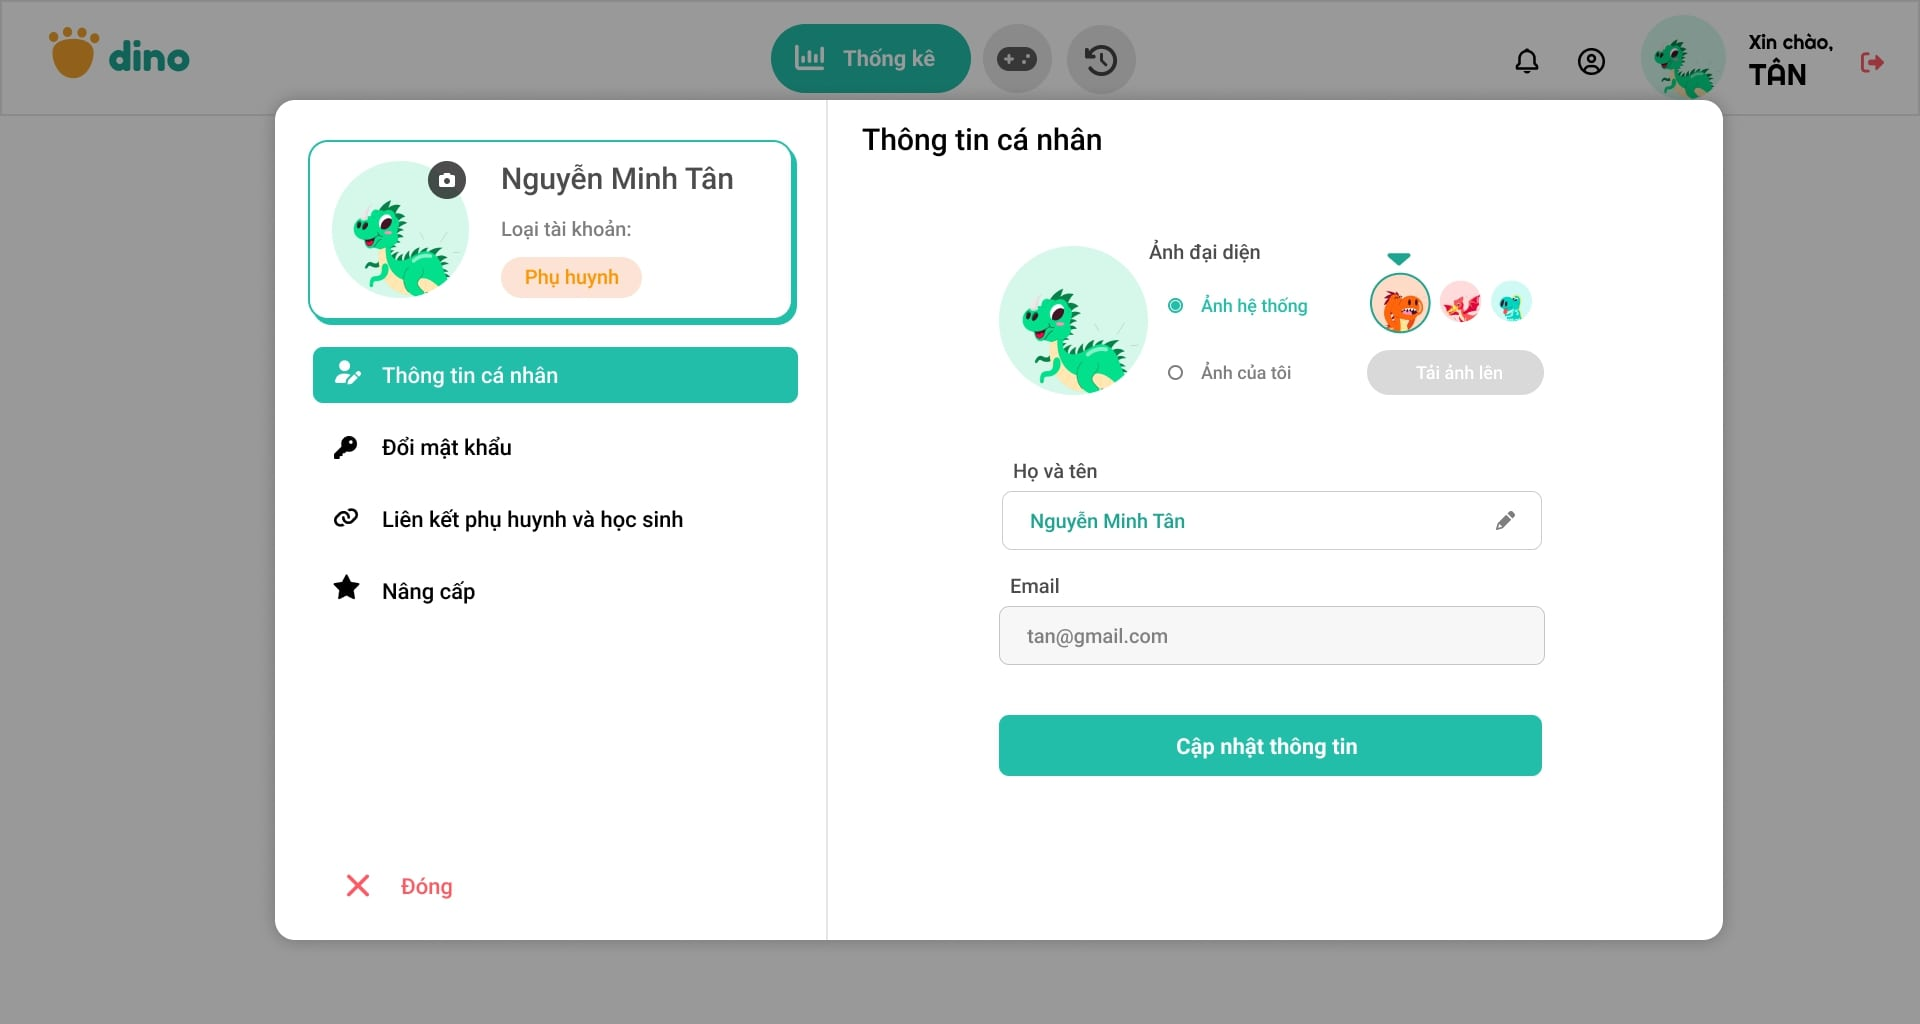
\includegraphics[width=0.9\textwidth]{Image/UI/Main-Parent/Info.jpg}
			\vspace{0.6cm}
			\caption{Quản lý tài khoản cá nhân - Xem và cập nhật thông tin}
		\end{figure}
	
	\item \textbf{Thay đổi mật khẩu}: Giao diện thay đổi mật khẩu của phụ huynh được thiết kế tương tự với giao diện của Học sinh. Thiết kế được mô tả chi tiết ở mục \ref{subsubsec:profile}.
	\newpage
	\item \textbf{Liên kết tài khoản}
	\vspace{0.1cm}
	\newline
		Phụ huynh có thể xem danh sách các tài khoản học sinh đã được liên kết vào Family như \textit{Hình \ref{fig:linked}}.
		\begin{figure}[H]
			\centering
			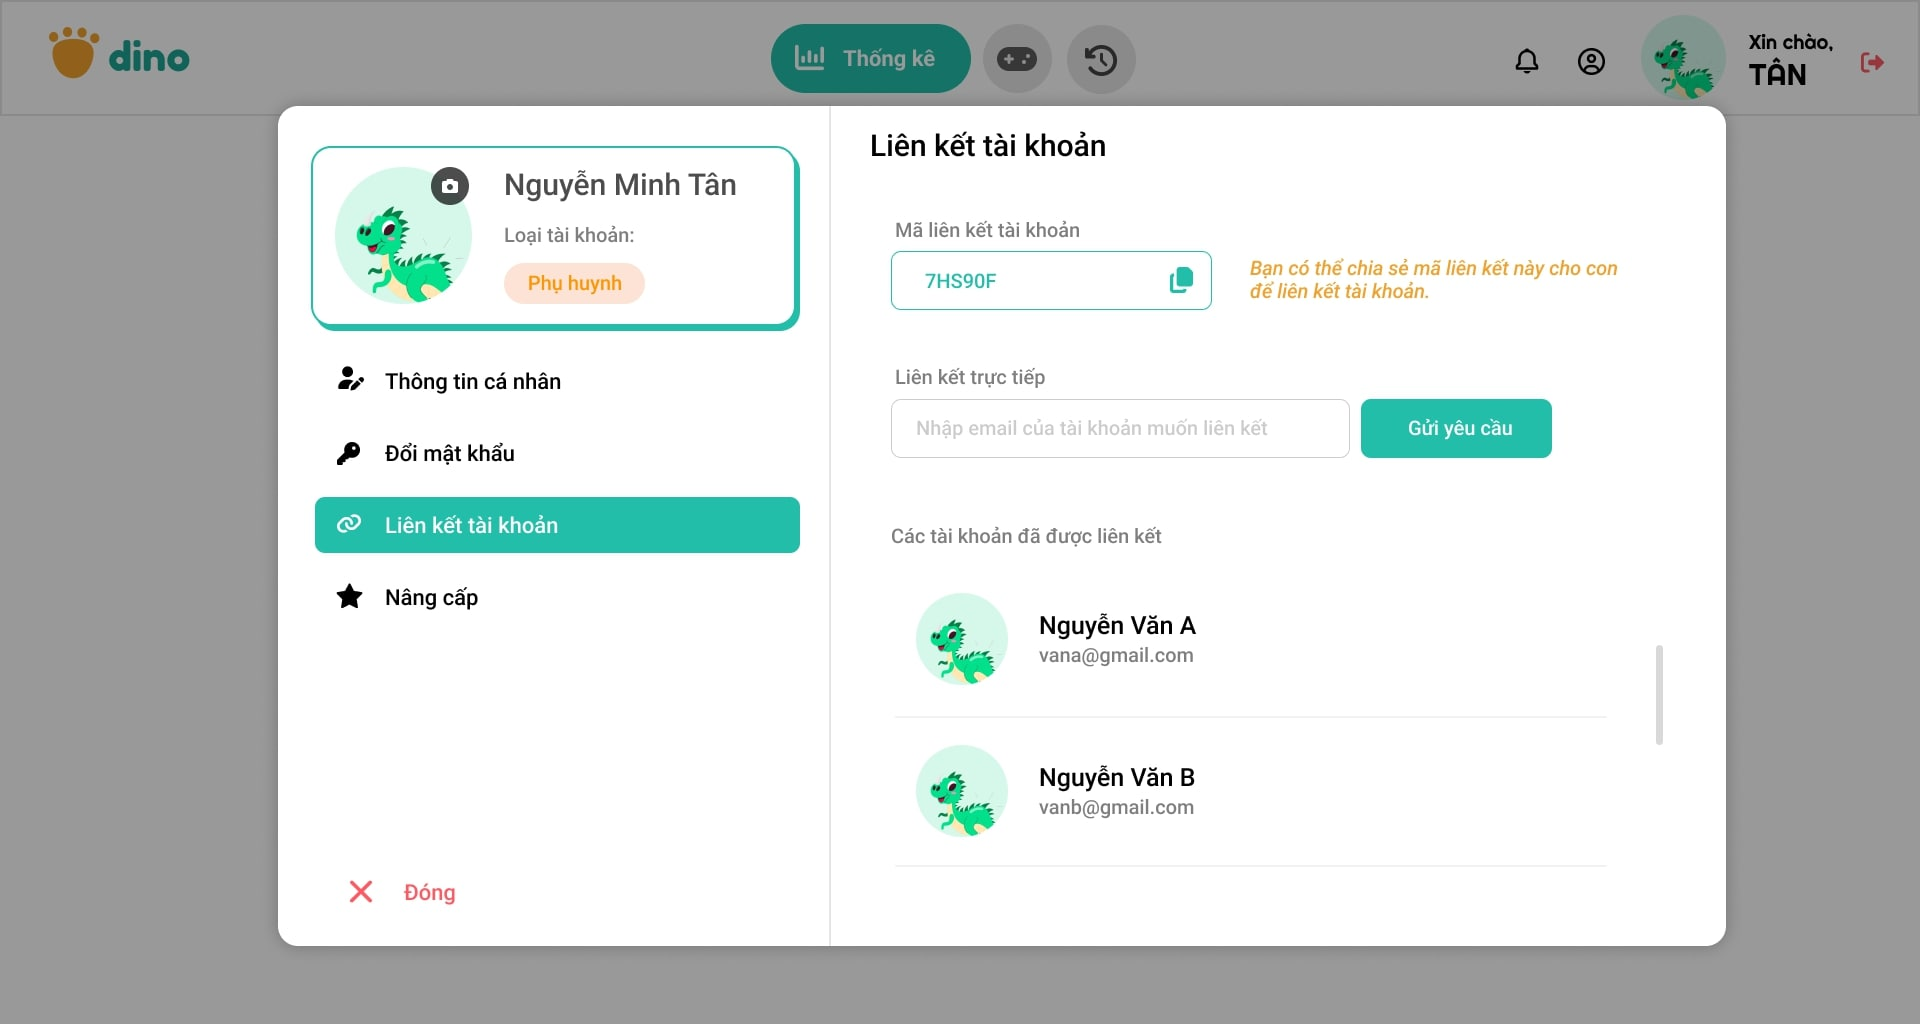
\includegraphics[width=0.9\textwidth]{Image/UI/Main-Parent/Account-Linked.jpg}
			\vspace{0.6cm}
			\caption{Quản lý tài khoản cá nhân - Đã liên kết tài khoản}
			\label{fig:linked}
		\end{figure}
	
	\item \textbf{Nâng cấp tài khoản}
	\vspace{0.1cm}
	\newline
	Phụ huynh có thể nâng cấp tài khoản qua các bước sau:
		\begin{itemize}
			\item Bước 1: Chọn Gói nâng cấp muốn mua.
			\begin{figure}[H]
				\centering
				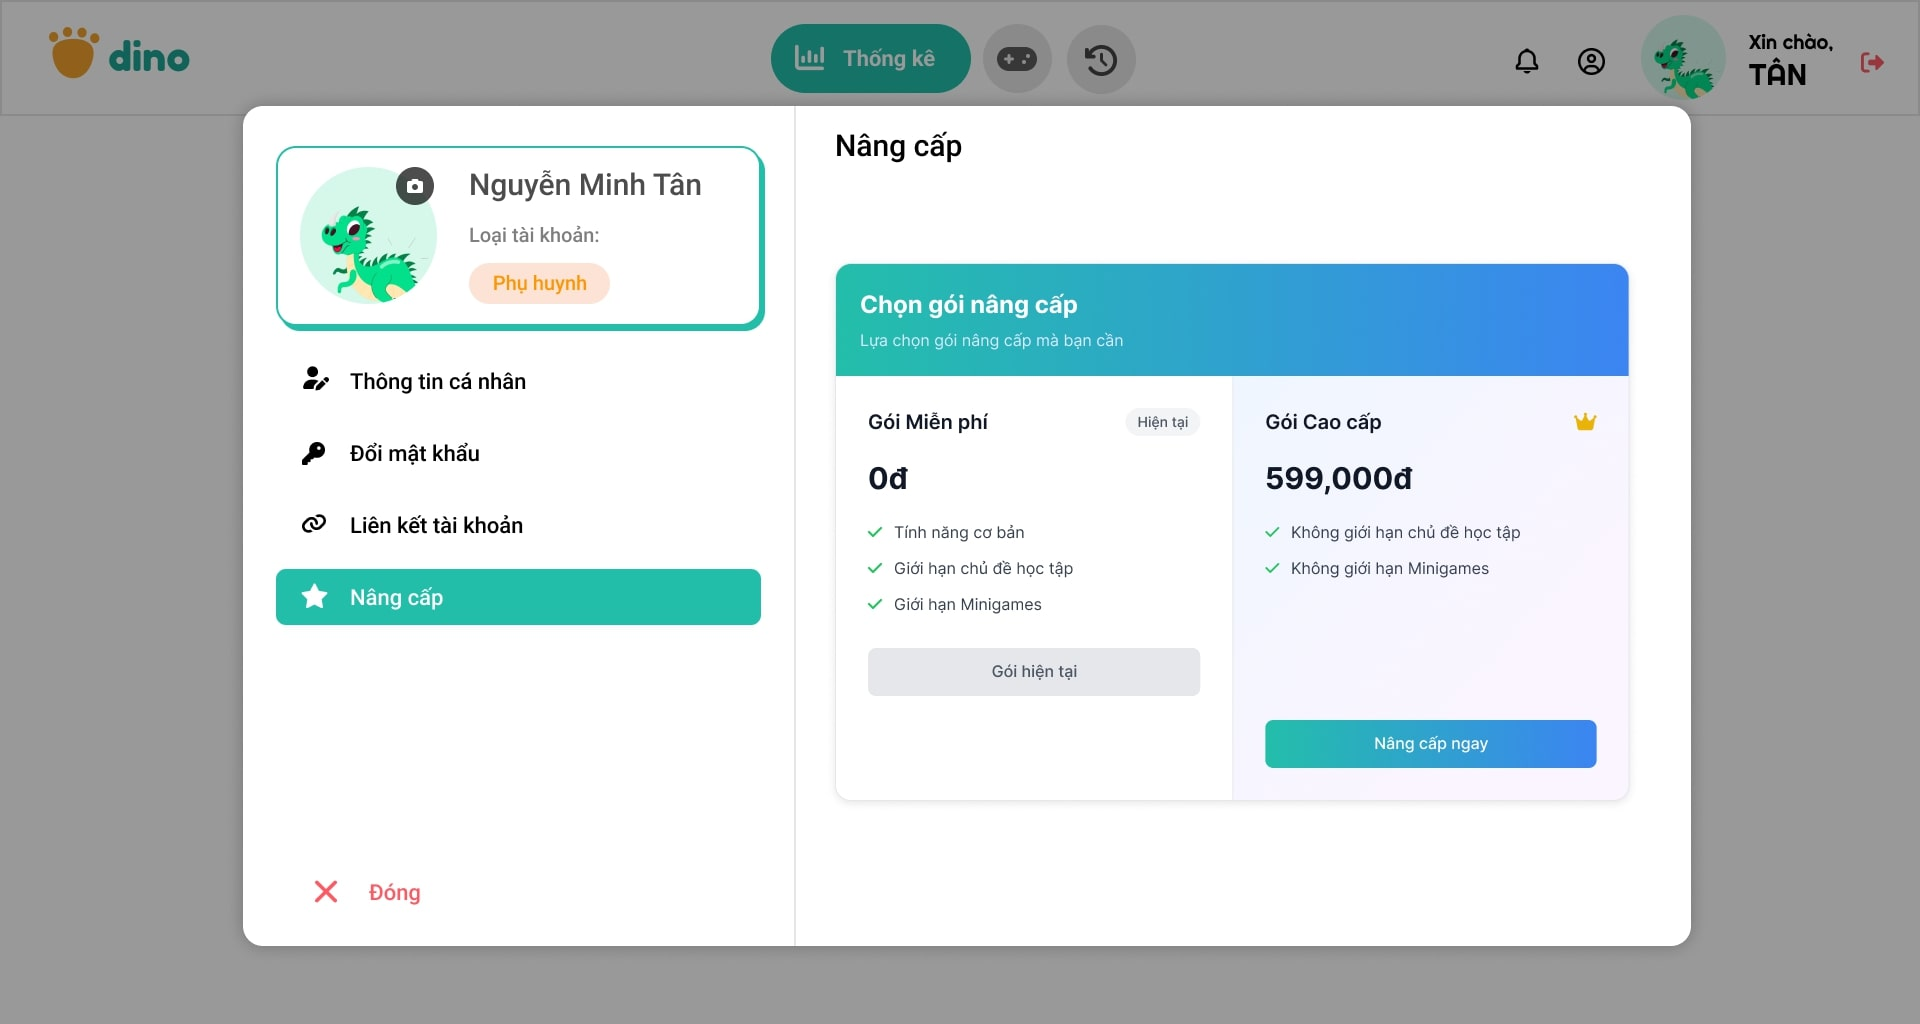
\includegraphics[width=0.9\textwidth]{Image/UI/Main-Parent/Plans.jpg}
				\vspace{0.6cm}
				\caption{Các gói nâng cấp}
			\end{figure}
			
			\item Bước 2: Thanh toán qua QRCode của VNPay.
			\begin{figure}[H]
				\centering
				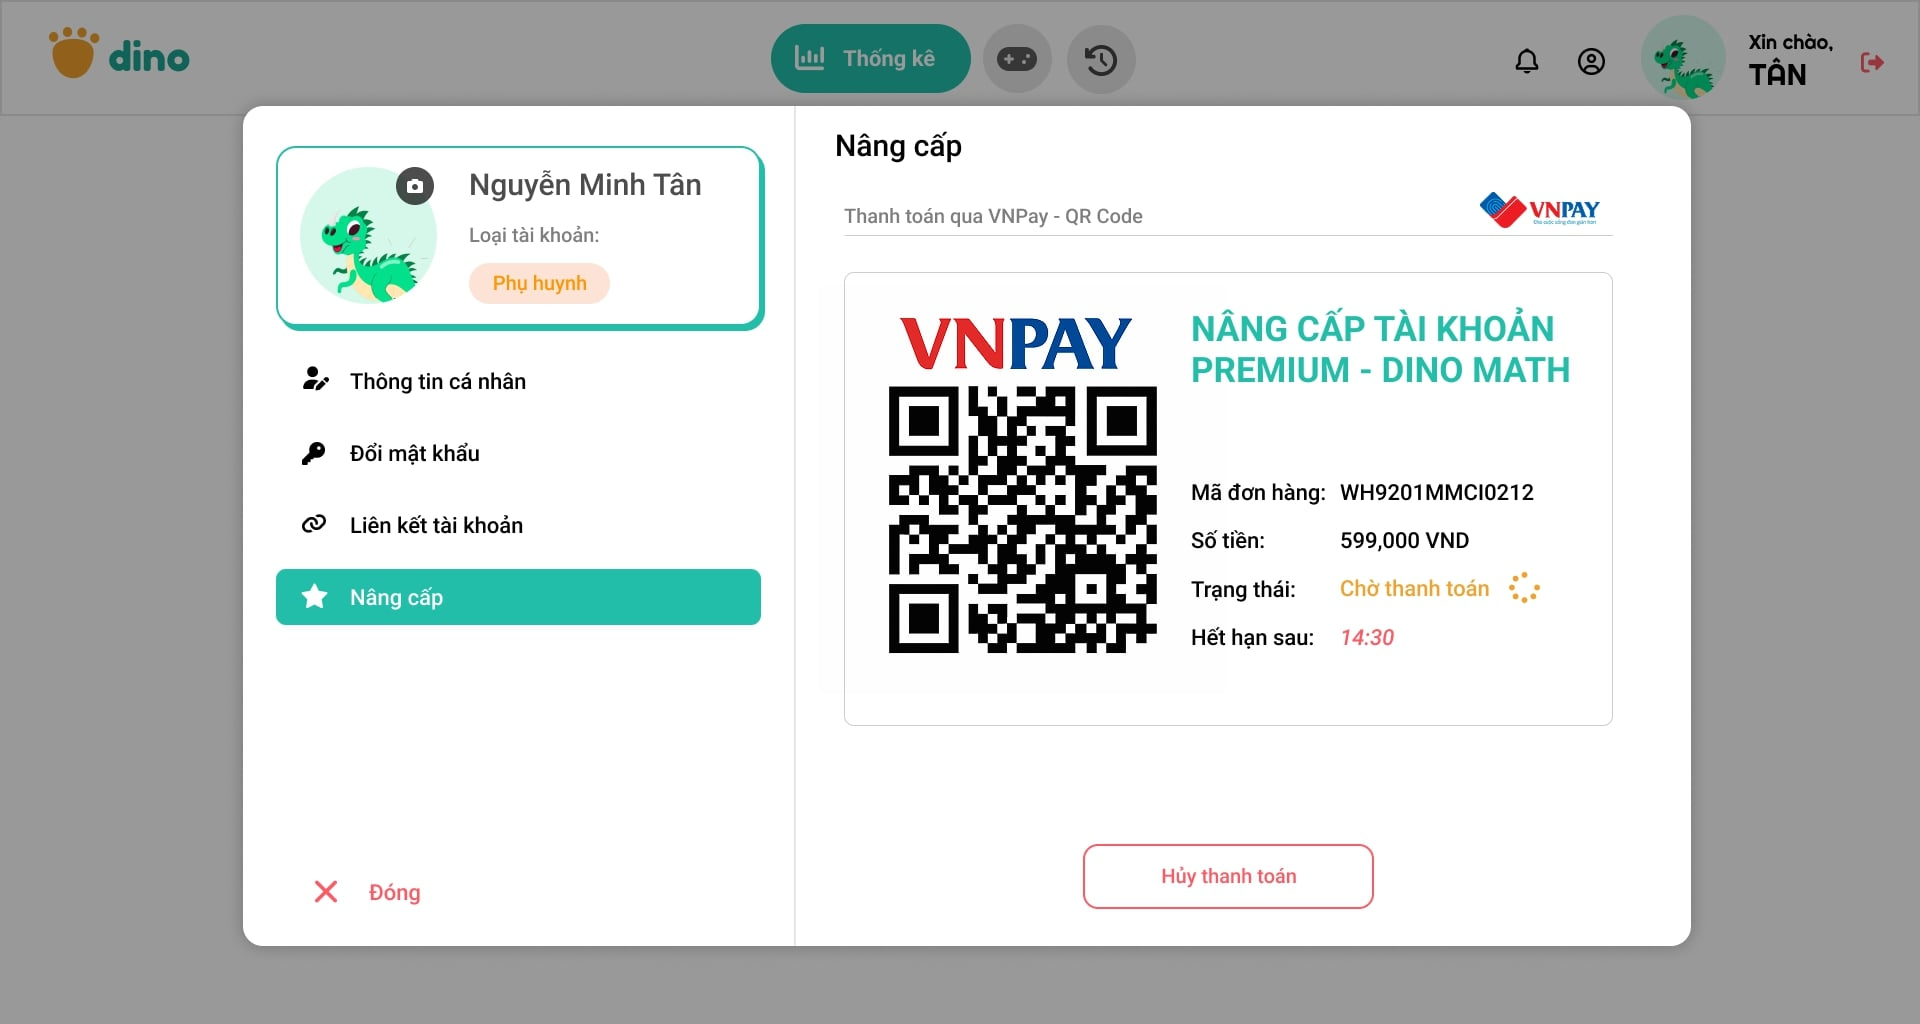
\includegraphics[width=0.9\textwidth]{Image/UI/Main-Parent/Payment-Loading.jpg}
				\vspace{0.6cm}
				\caption{Chờ xác nhận thanh toán}
			\end{figure}
			
			\item Bước 3: Sau khi thanh toán thành công, màn hình hiển thị trạng thái tài khoản đã nâng cấp và một số các phúc lợi của người dùng.
			\begin{figure}[H]
				\centering
				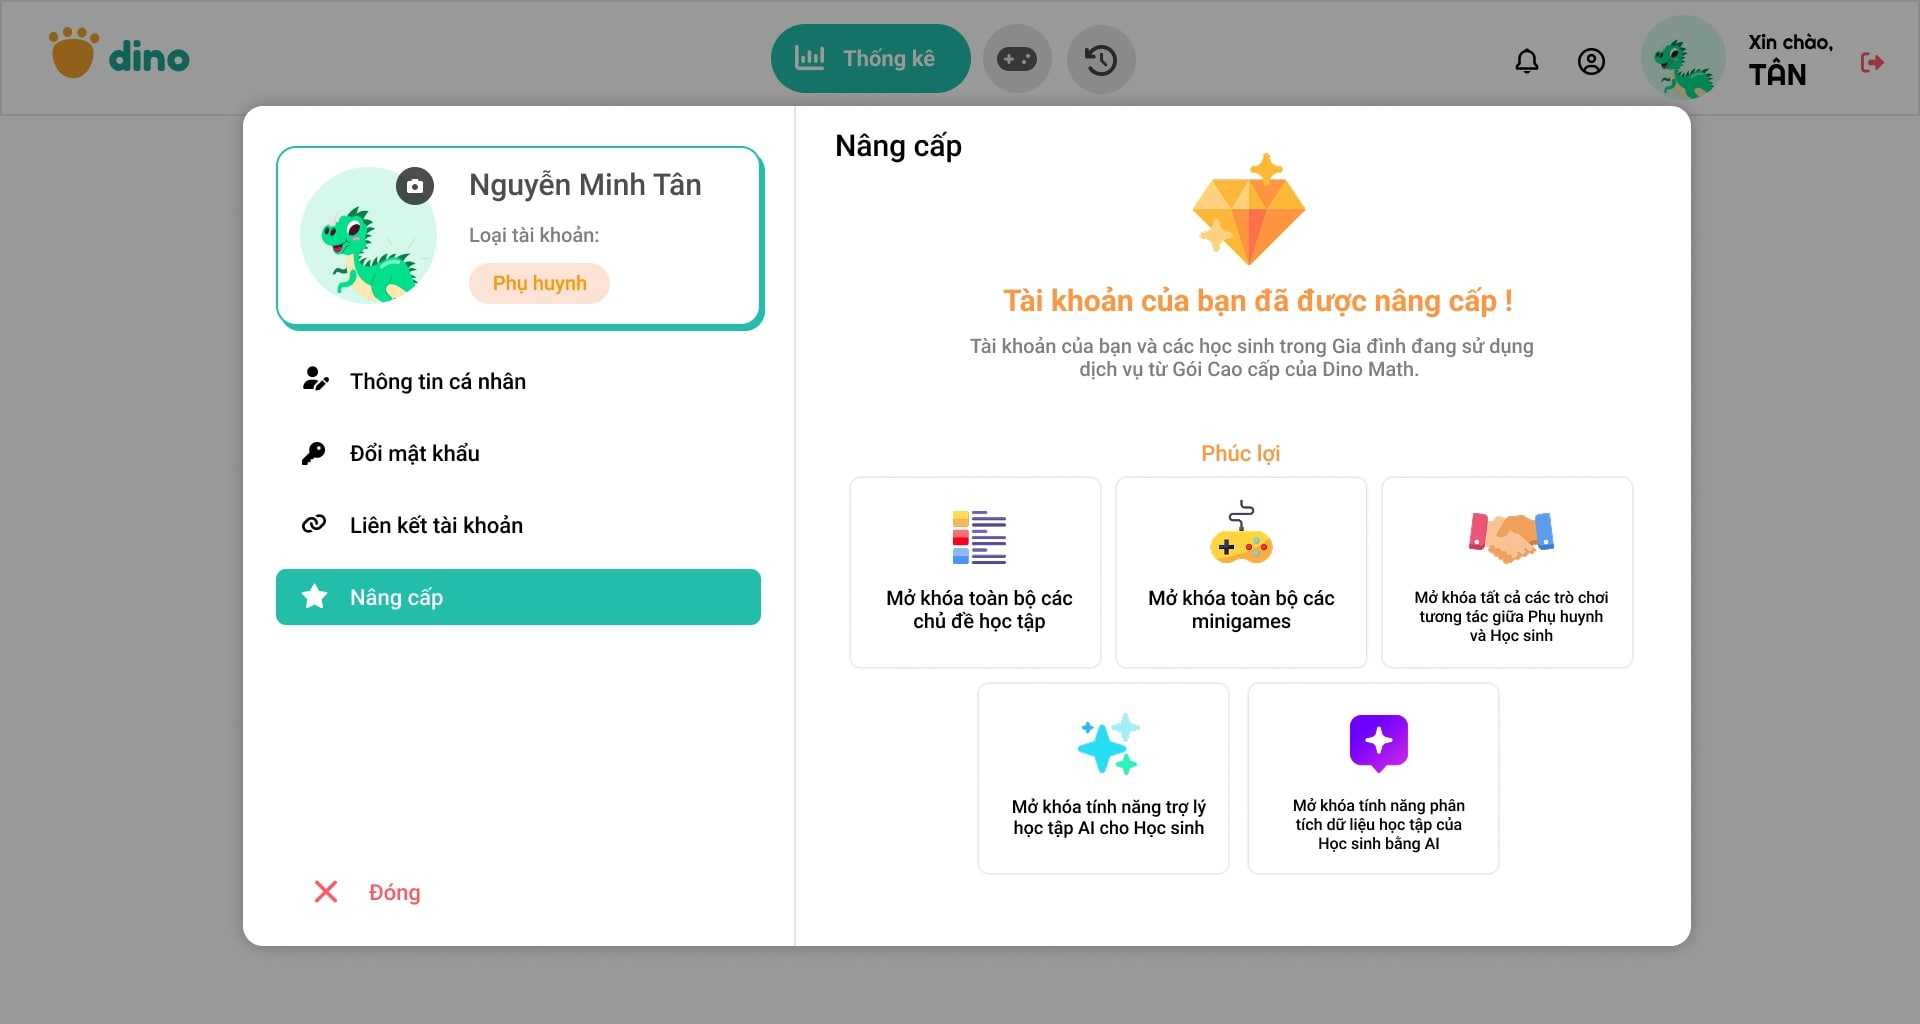
\includegraphics[width=0.9\textwidth]{Image/UI/Main-Parent/AfterPurchase.jpg}
				\vspace{0.6cm}
				\caption{Trạng thái tài khoản đã được nâng cấp}
			\end{figure}
		\end{itemize}
\end{enumerate}

\subsection{Các màn hình chính của quản trị viên (Admin)}

\subsubsection{Quản lý tài khoản}
Quản trị viên có thể xem danh sách tài khoản người dùng và thực hiện khoá hoặc mở khoá tài khoản.
\begin{figure}[H]
	\centering
	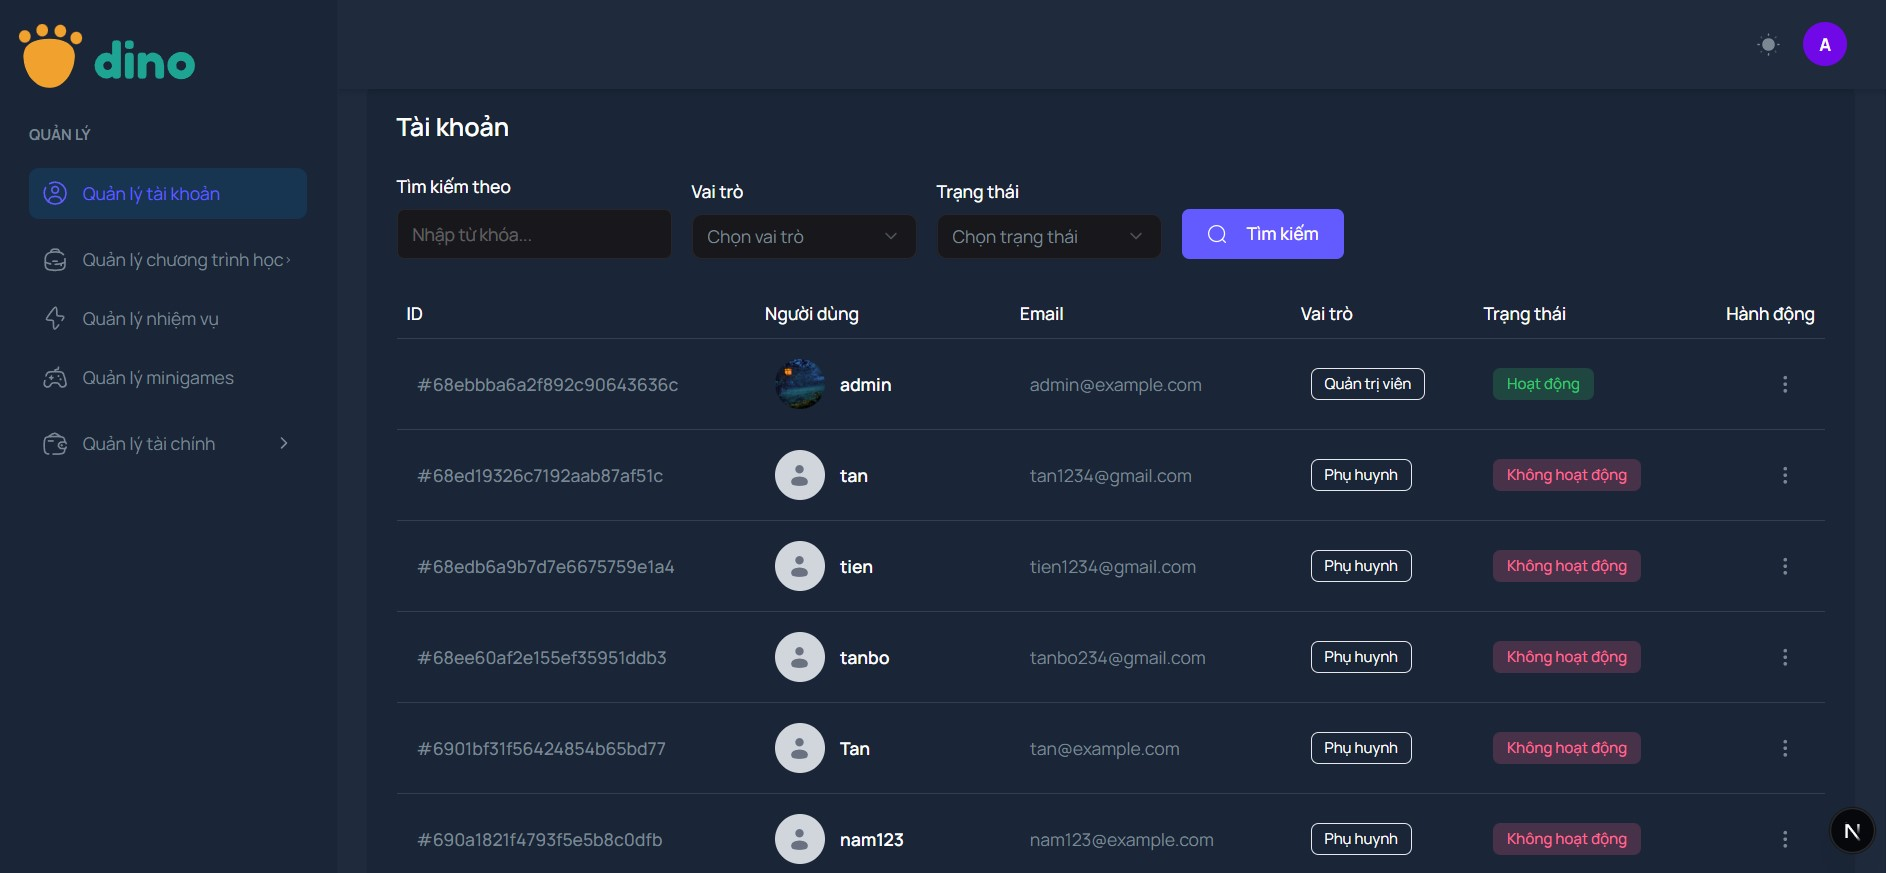
\includegraphics[width=0.9\textwidth]{Image/UI/Admin/Account.jpg}
	\vspace{0.6cm}
	\caption{Admin - Quản lý tài khoản}
\end{figure}

\subsubsection{Quản lý học kỳ}
Quản trị viên có thể tạo và quản lý các học kỳ trong năm học, làm cơ sở để gắn kết bài kiểm tra đầu vào và các hoạt động theo từng giai đoạn học tập.
\begin{figure}[H]
	\centering
	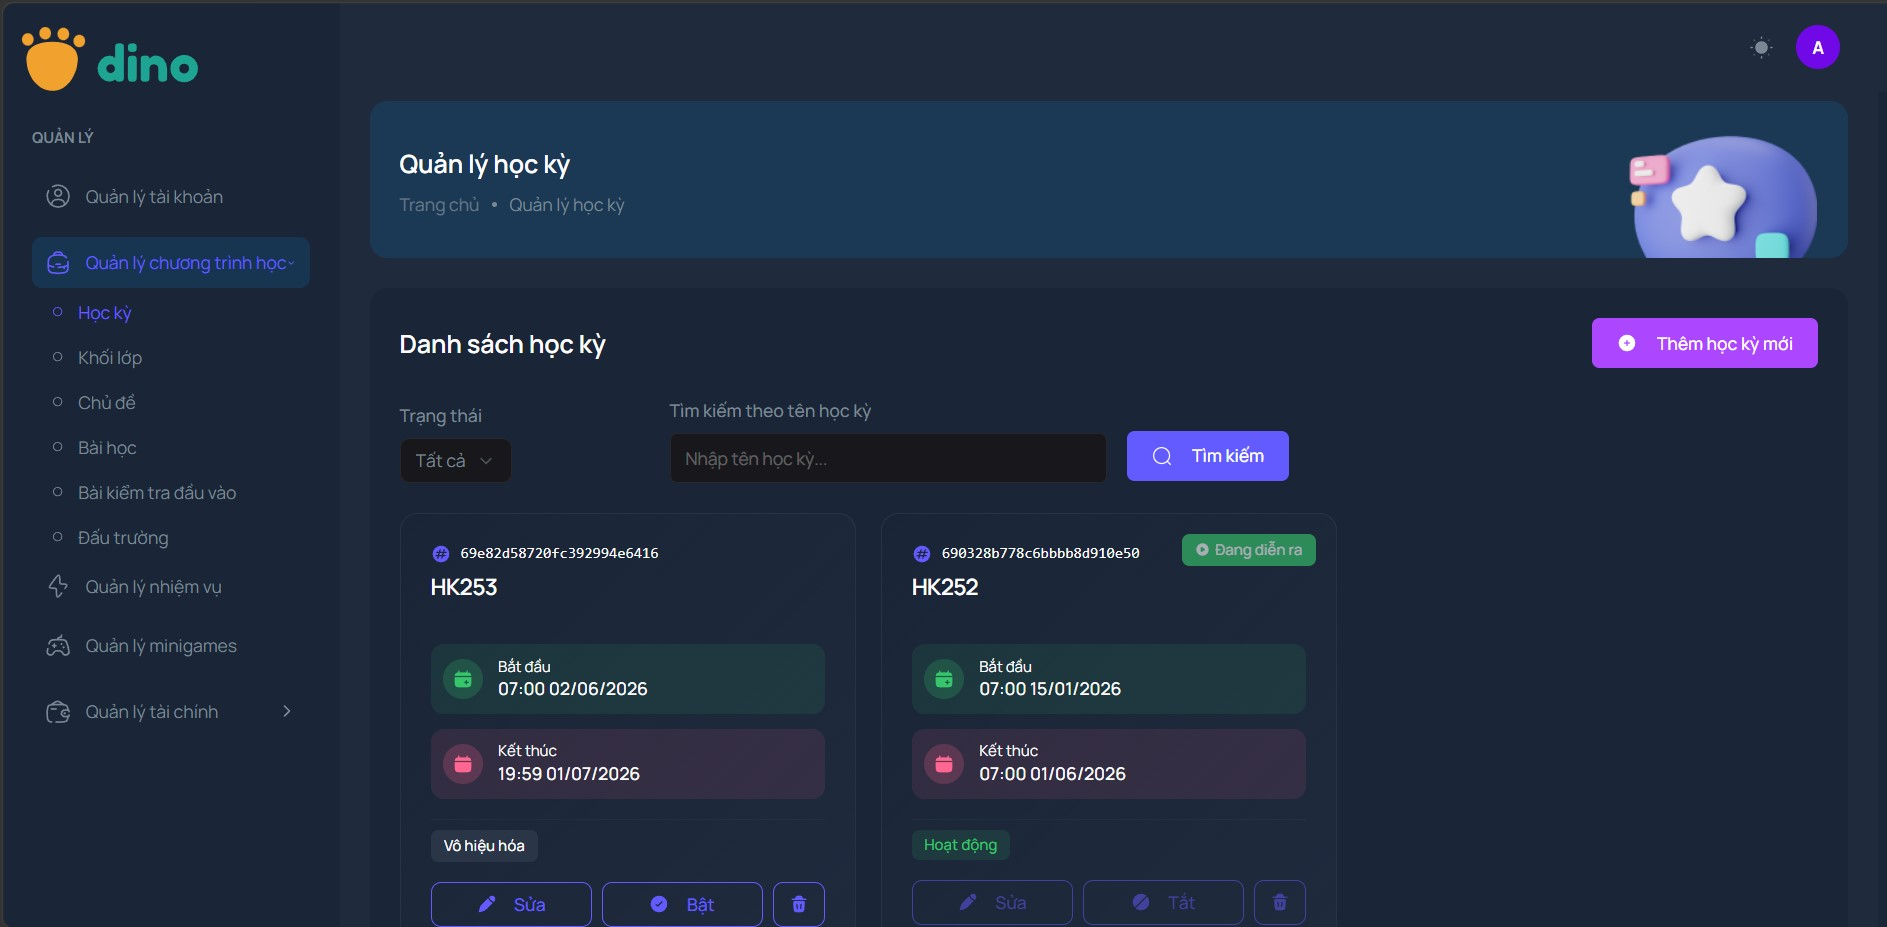
\includegraphics[width=0.9\textwidth]{Image/UI/Admin/Semester.jpg}
	\vspace{0.6cm}
	\caption{Admin - Quản lý học kỳ}
\end{figure}

\subsubsection{Quản lý khối lớp}
Quản trị viên có thể xem và chỉnh sửa các khối lớp (Lớp 1--5). Mỗi khối lớp gắn liền với một thế giới riêng, trong đó bao gồm các vùng đất tương ứng với từng chủ đề học.
\begin{figure}[H]
	\centering
	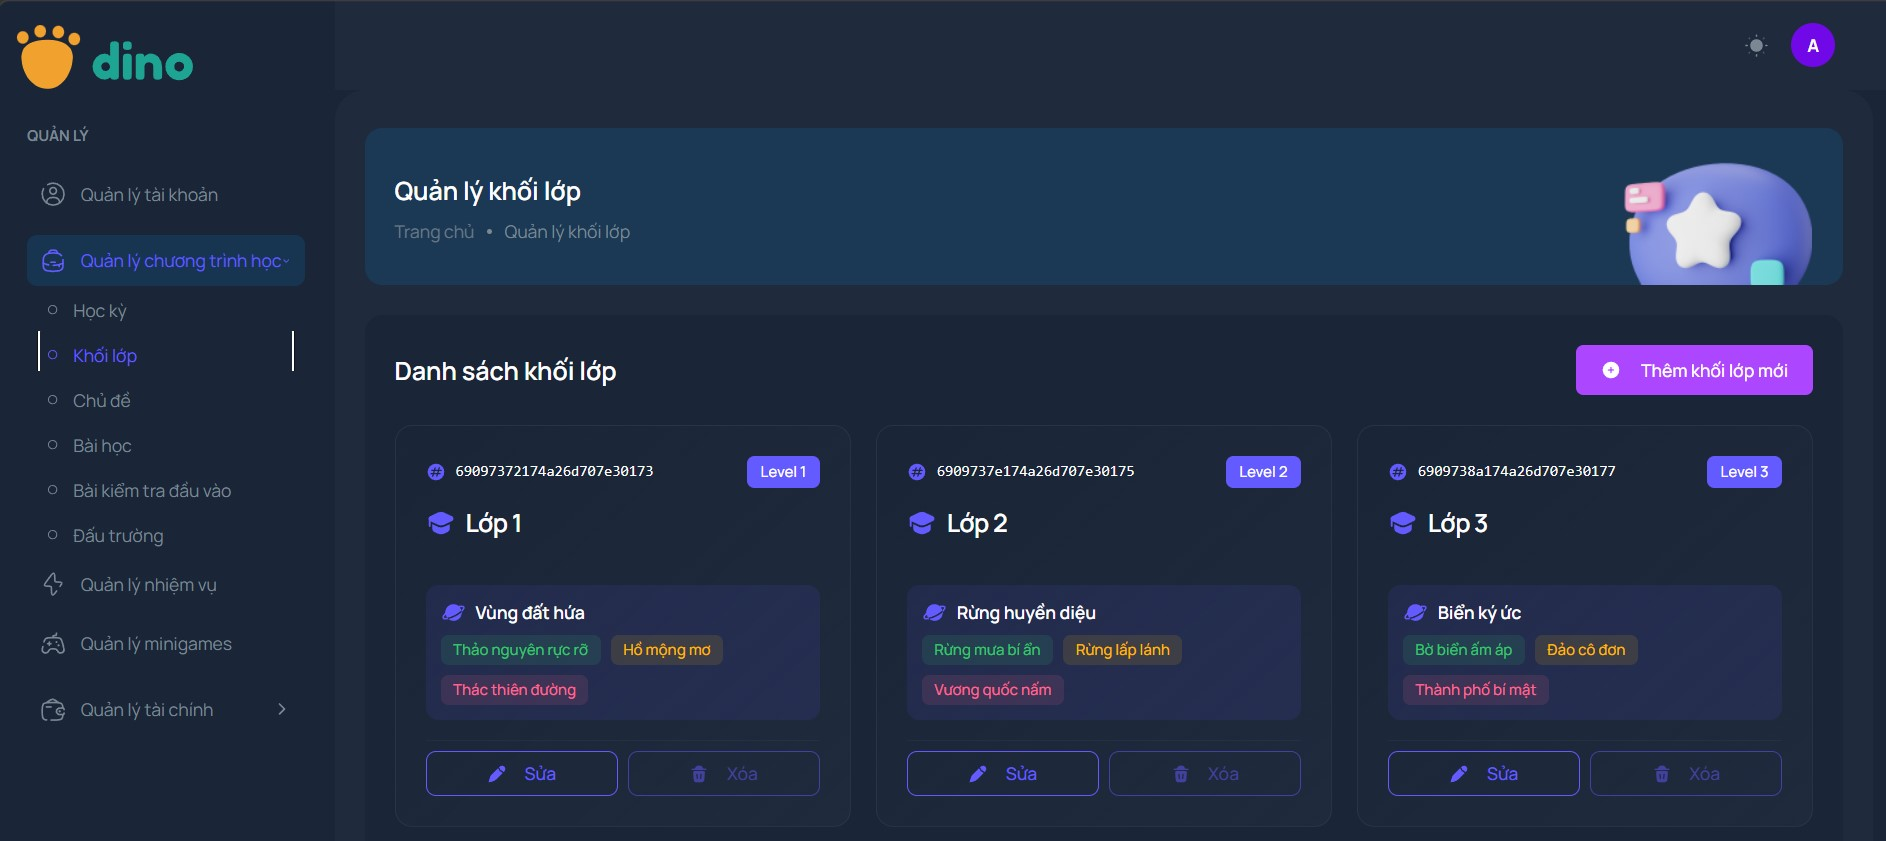
\includegraphics[width=0.9\textwidth]{Image/UI/Admin/Grade.jpg}
	\vspace{0.6cm}
	\caption{Admin - Quản lý khối lớp}
\end{figure}

\subsubsection{Quản lý bài học}
Quản trị viên có thể xem, tìm kiếm và lọc danh sách bài học theo chủ đề và độ khó. Hệ thống hỗ trợ thêm mới bài học, xóa bài học theo chủ đề, và xuất định dạng Excel mẫu để nhập liệu hàng loạt.
\begin{figure}[H]
	\centering
	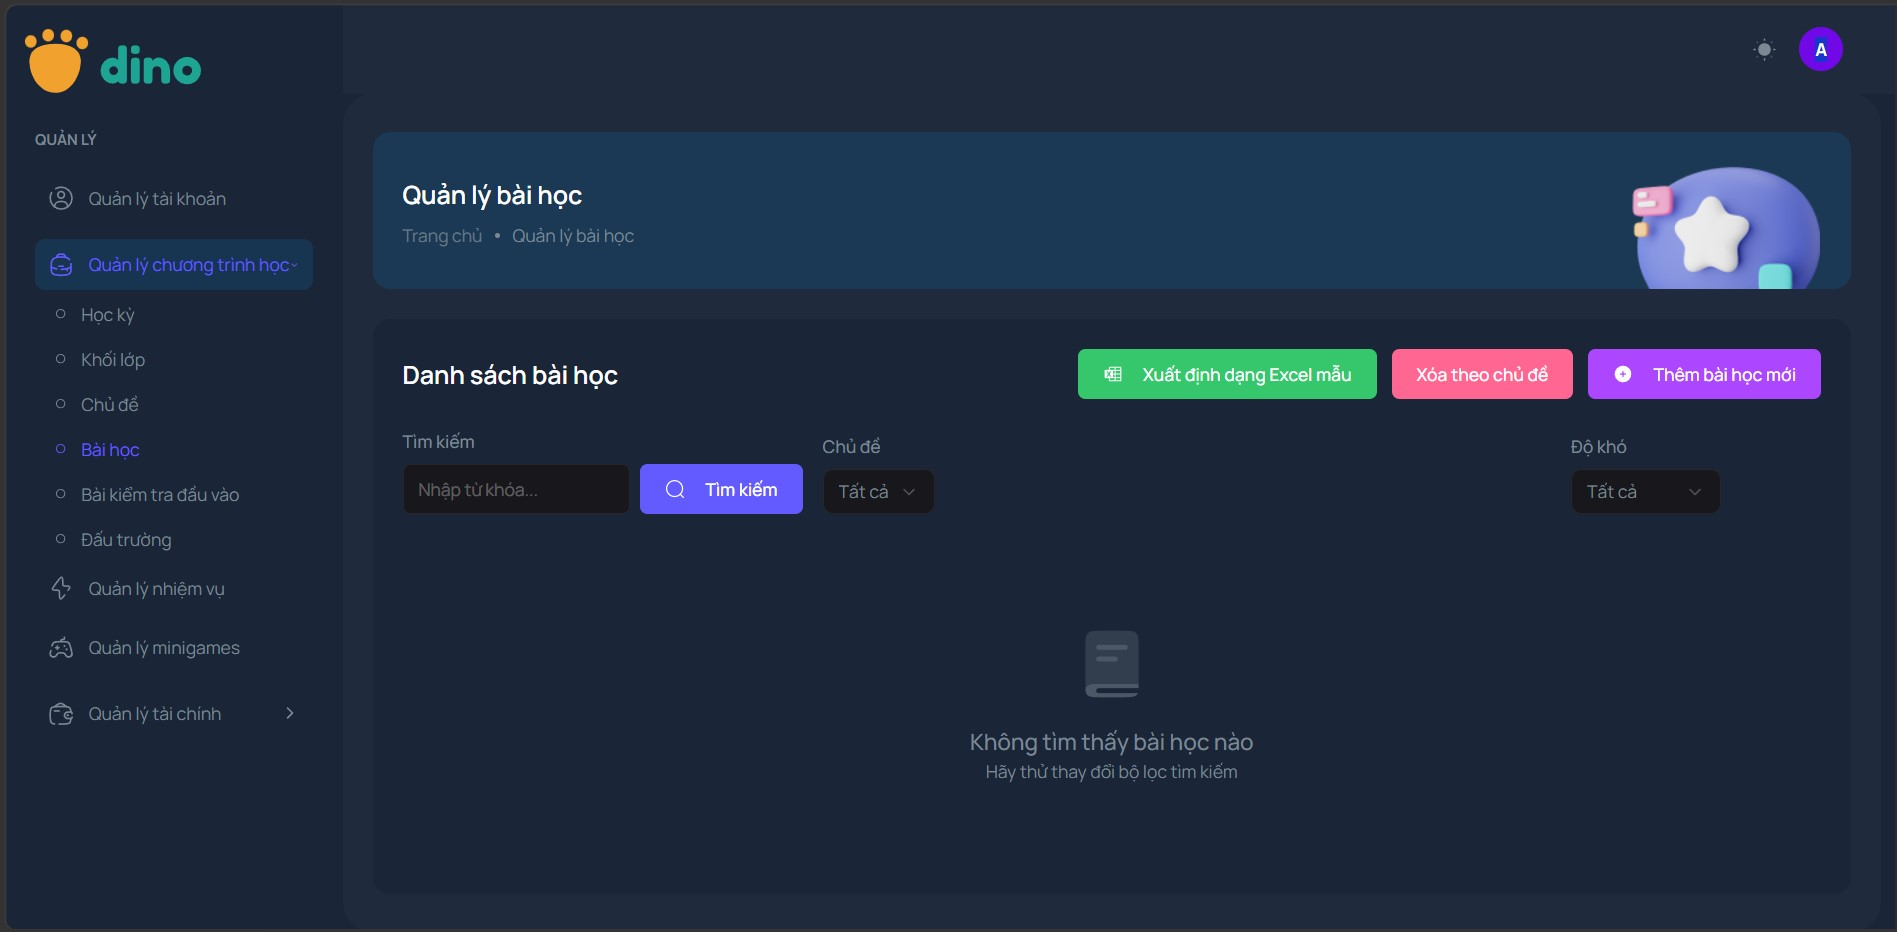
\includegraphics[width=0.9\textwidth]{Image/UI/Admin/Lesson.jpg}
	\vspace{0.6cm}
	\caption{Admin - Quản lý bài học}
\end{figure}

\subsubsection{Quản lý bài tập}
Quản trị viên có thể tạo, chỉnh sửa và xoá nội dung bài tập, tổ chức theo chủ đề và bài học.
\begin{figure}[H]
	\centering
	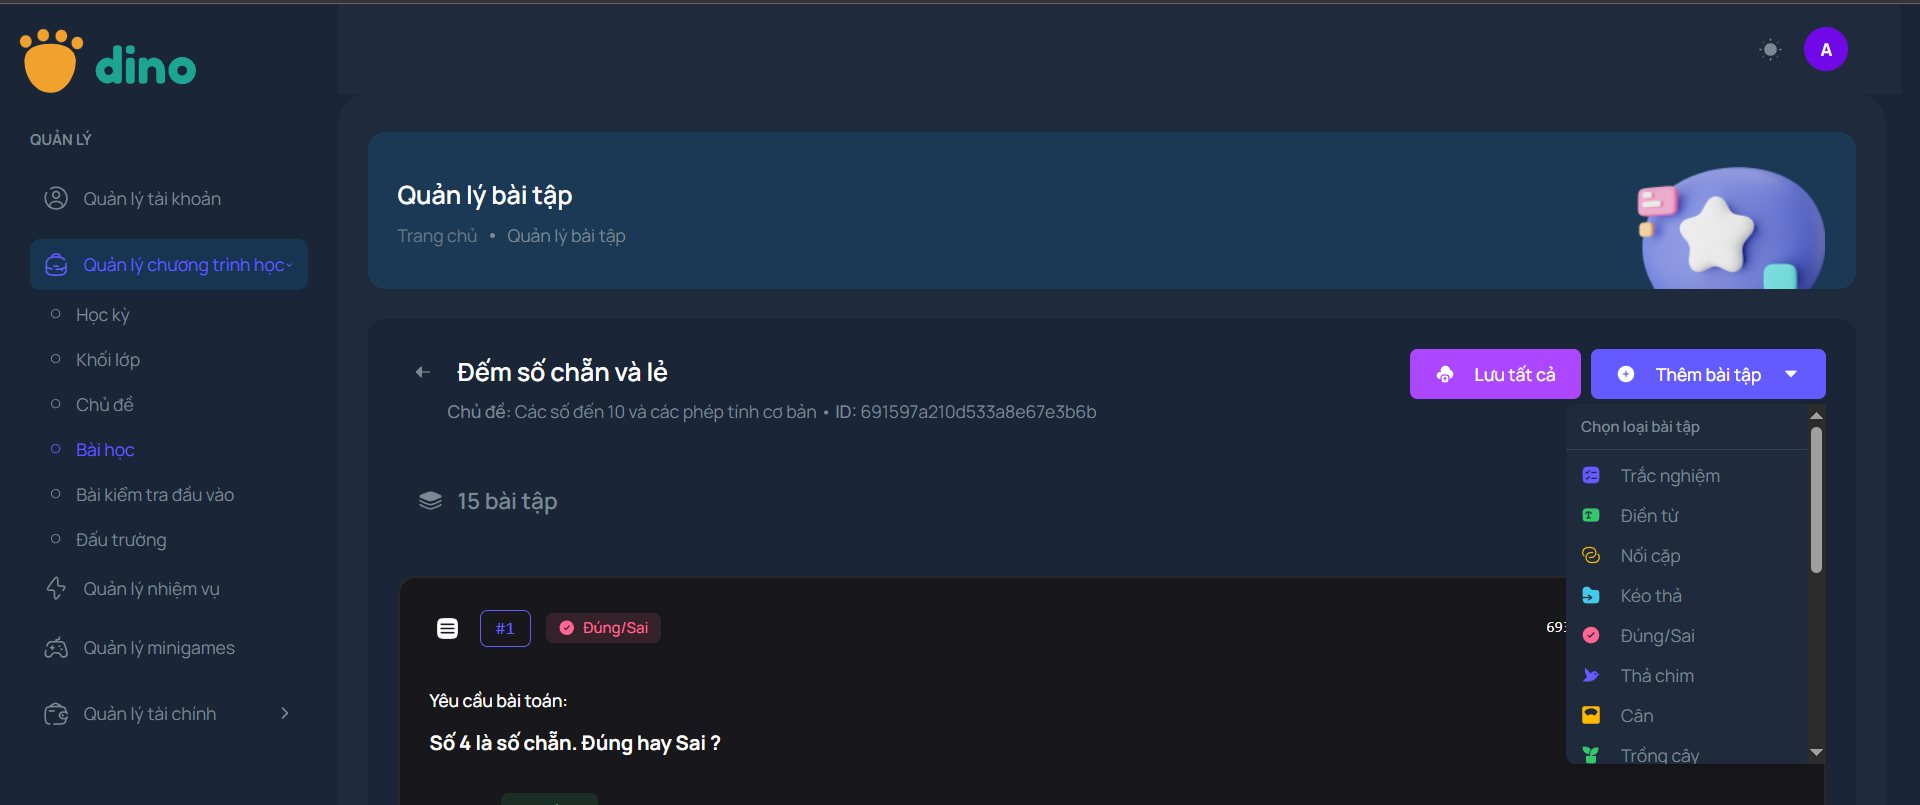
\includegraphics[width=0.9\textwidth]{Image/UI/Admin/Exercise.jpg}
	\vspace{0.6cm}
	\caption{Admin - Quản lý bài tập}
\end{figure}

Khi thêm mới hoặc chỉnh sửa bài tập, hệ thống cung cấp hai phương thức nhập liệu linh hoạt như sau:
\begin{itemize}
	\item \textbf{Nhập liệu qua form:} Mỗi dạng bài tập (trắc nghiệm, kéo thả, điền khuyết, nối, đúng/sai,...) có một form nhập câu hỏi đặc trưng riêng, bao gồm các trường thông tin phù hợp với cấu trúc dữ liệu của từng dạng. Quản trị viên chỉ cần điền vào các trường tương ứng mà không cần hiểu cấu trúc dữ liệu bên dưới.
	\item \textbf{Nhập liệu qua JSON:} Đối với người dùng có kinh nghiệm kỹ thuật hoặc khi cần nhập hàng loạt, hệ thống hỗ trợ nhập dữ liệu trực tiếp dưới dạng JSON theo schema quy định sẵn cho từng loại bài tập. Phương thức này giúp tăng tốc độ tạo nội dung đáng kể.
\end{itemize}

Ngoài ra, trước khi lưu bài tập, quản trị viên có thể sử dụng chức năng \textbf{Xem trước (Preview)} để kiểm tra giao diện và trải nghiệm bài tập đúng như cách học sinh sẽ thấy. Tính năng này giúp phát hiện sớm các lỗi về nội dung, hình ảnh hoặc logic tương tác trước khi bài tập được công bố chính thức trên hệ thống.

\subsubsection{Quản lý bài kiểm tra đầu vào}
Quản trị viên có thể tạo, chỉnh sửa và công bố các bài kiểm tra đầu vào theo từng khối lớp. Mỗi bài kiểm tra có thể được lọc theo khối lớp và bật/tắt trạng thái công bố.
\begin{figure}[H]
	\centering
	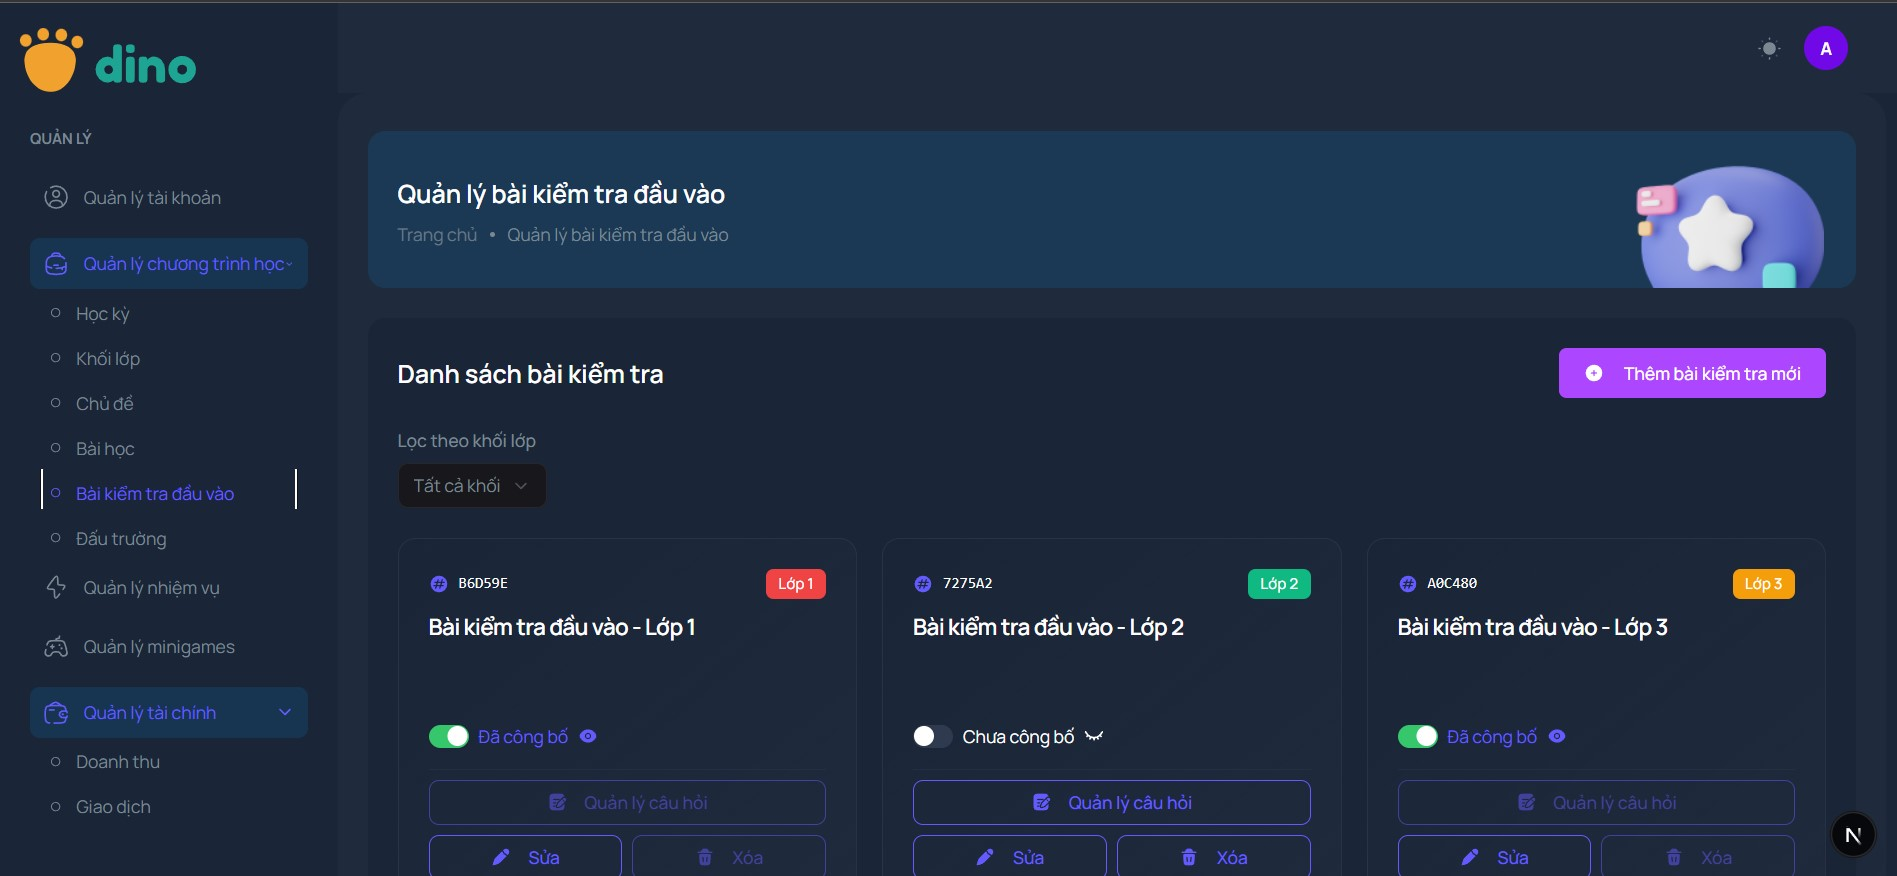
\includegraphics[width=0.9\textwidth]{Image/UI/Admin/Test.jpg}
	\vspace{0.6cm}
	\caption{Admin - Quản lý bài kiểm tra đầu vào}
\end{figure}

\subsubsection{Quản lý đấu trường}
Quản trị viên có thể tạo và quản lý các đấu trường theo tuần. Mỗi đấu trường có thể được lọc theo khối lớp và trạng thái, đồng thời hỗ trợ thiết lập thời gian bắt đầu và kết thúc cụ thể.
\begin{figure}[H]
	\centering
	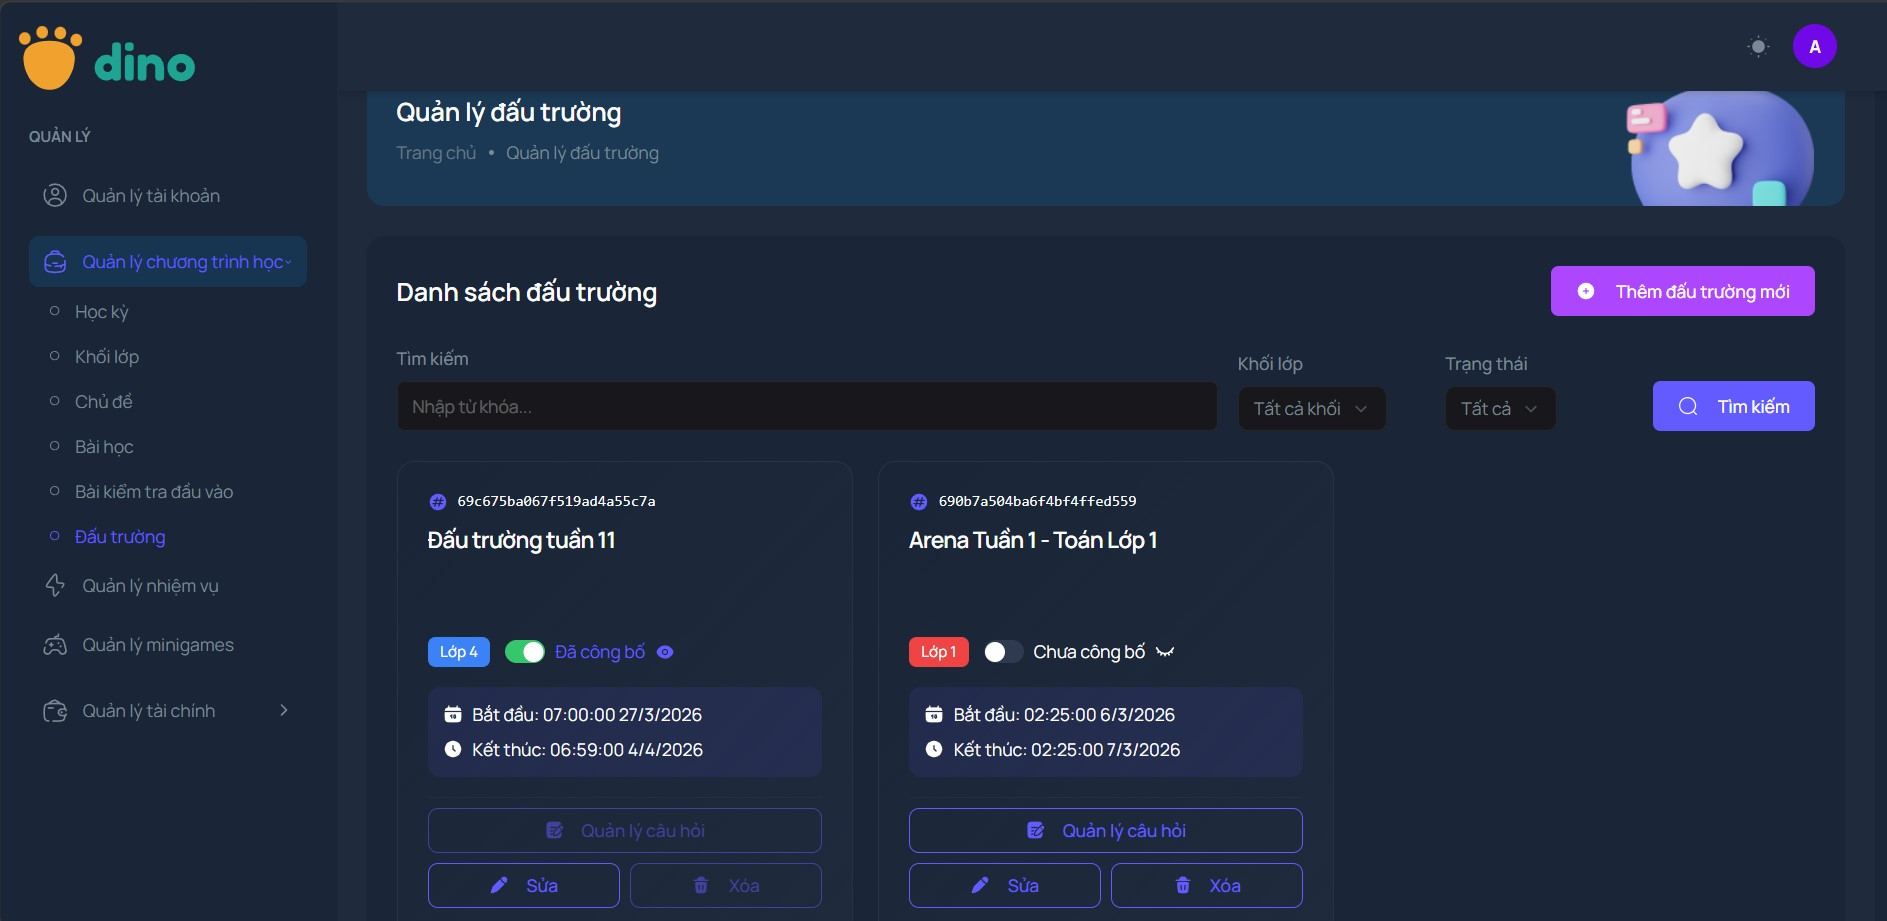
\includegraphics[width=0.9\textwidth]{Image/UI/Admin/Arena.jpg}
	\vspace{0.6cm}
	\caption{Admin - Quản lý đấu trường}
\end{figure}

\subsubsection{Quản lý nhiệm vụ}
Quản trị viên có thể tạo nhiệm vụ hằng ngày, thiết lập điều kiện hoàn thành và phần thưởng tương ứng.
\begin{figure}[H]
	\centering
	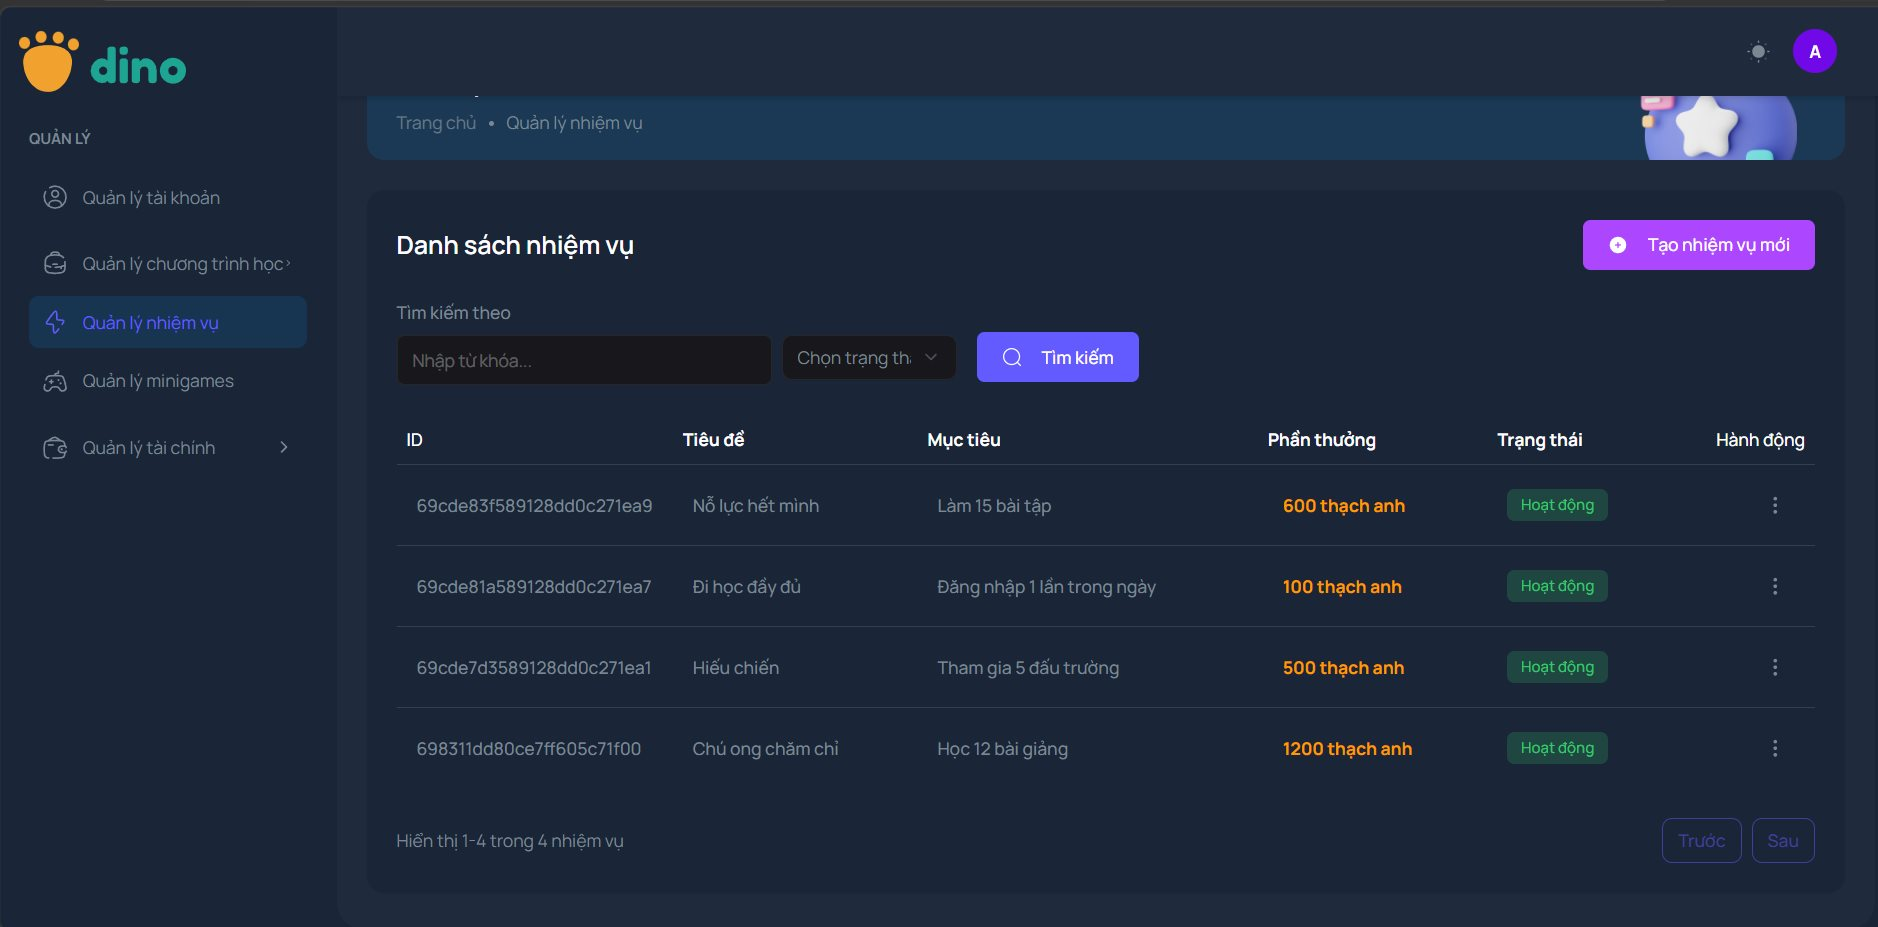
\includegraphics[width=0.9\textwidth]{Image/UI/Admin/Missions.jpg}
	\vspace{0.6cm}
	\caption{Admin - Quản lý nhiệm vụ}
\end{figure}

\subsubsection{Quản lý Minigames}
Quản trị viên có thể tạo và chỉnh sửa nội dung các minigame trong hệ thống.
\begin{figure}[H]
	\centering
	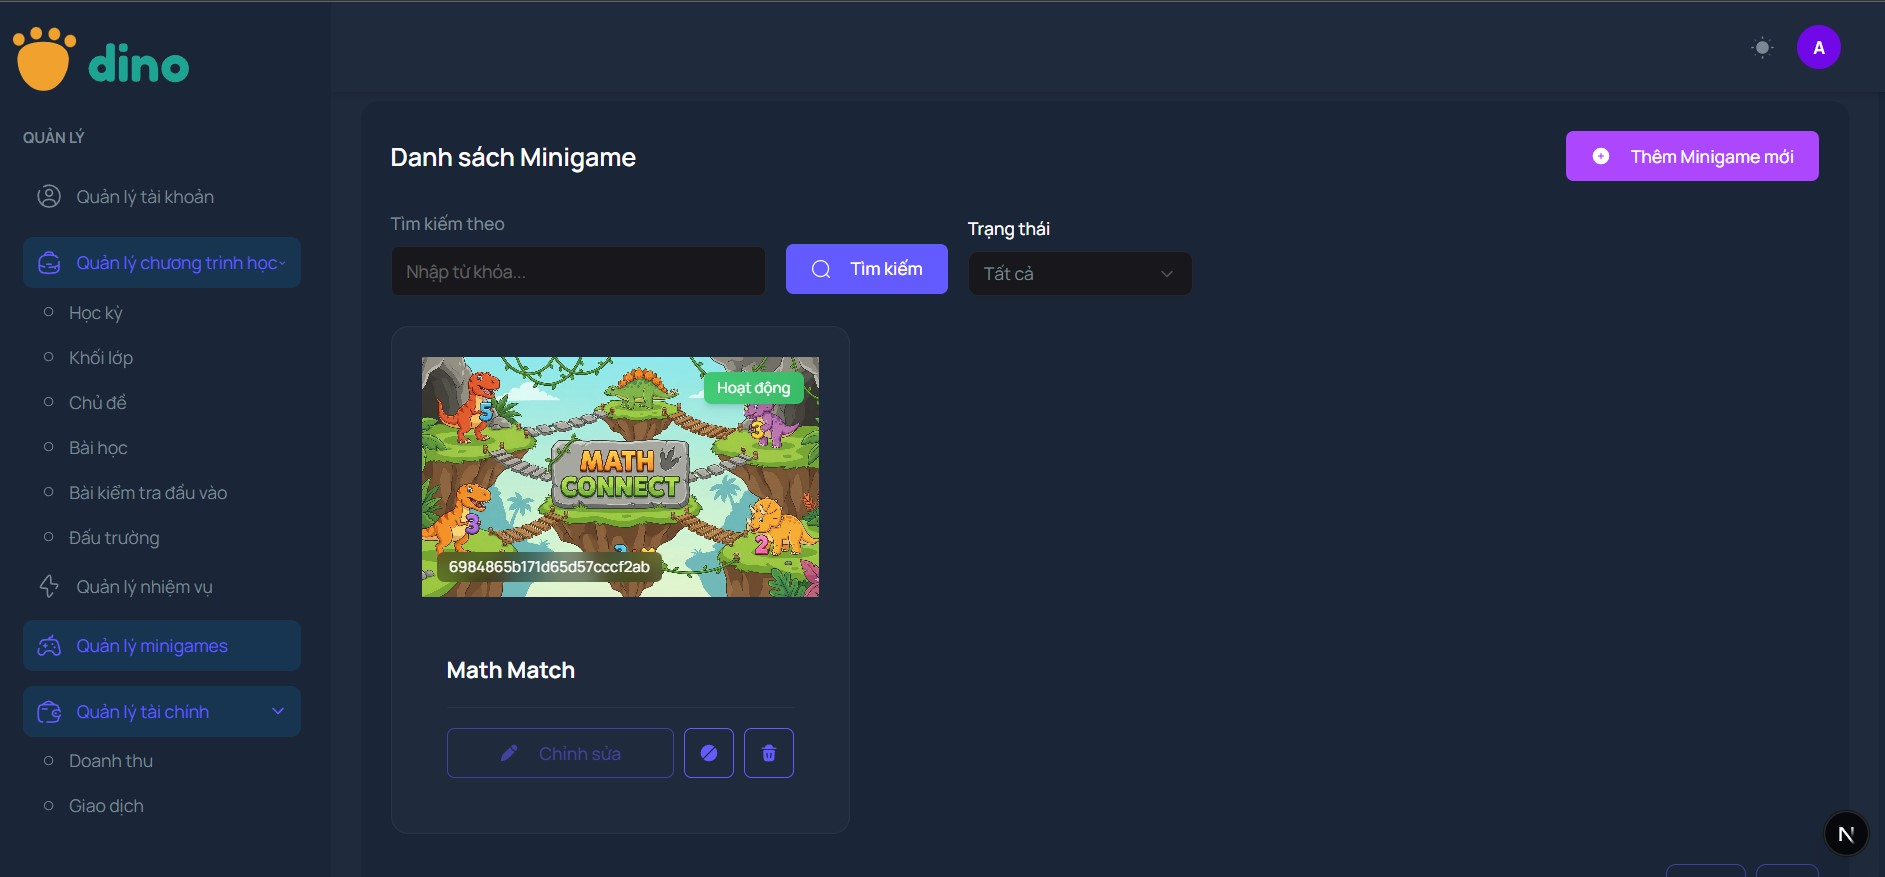
\includegraphics[width=0.9\textwidth]{Image/UI/Admin/Minigame.jpg}
	\vspace{0.6cm}
	\caption{Admin - Quản lý Minigames}
\end{figure}

\subsubsection{Quản lý tài chính}
Quản trị viên có thể xem doanh thu của hệ thống và theo dõi, quản lý các giao dịch thanh toán.
\begin{figure}[H]
	\centering
	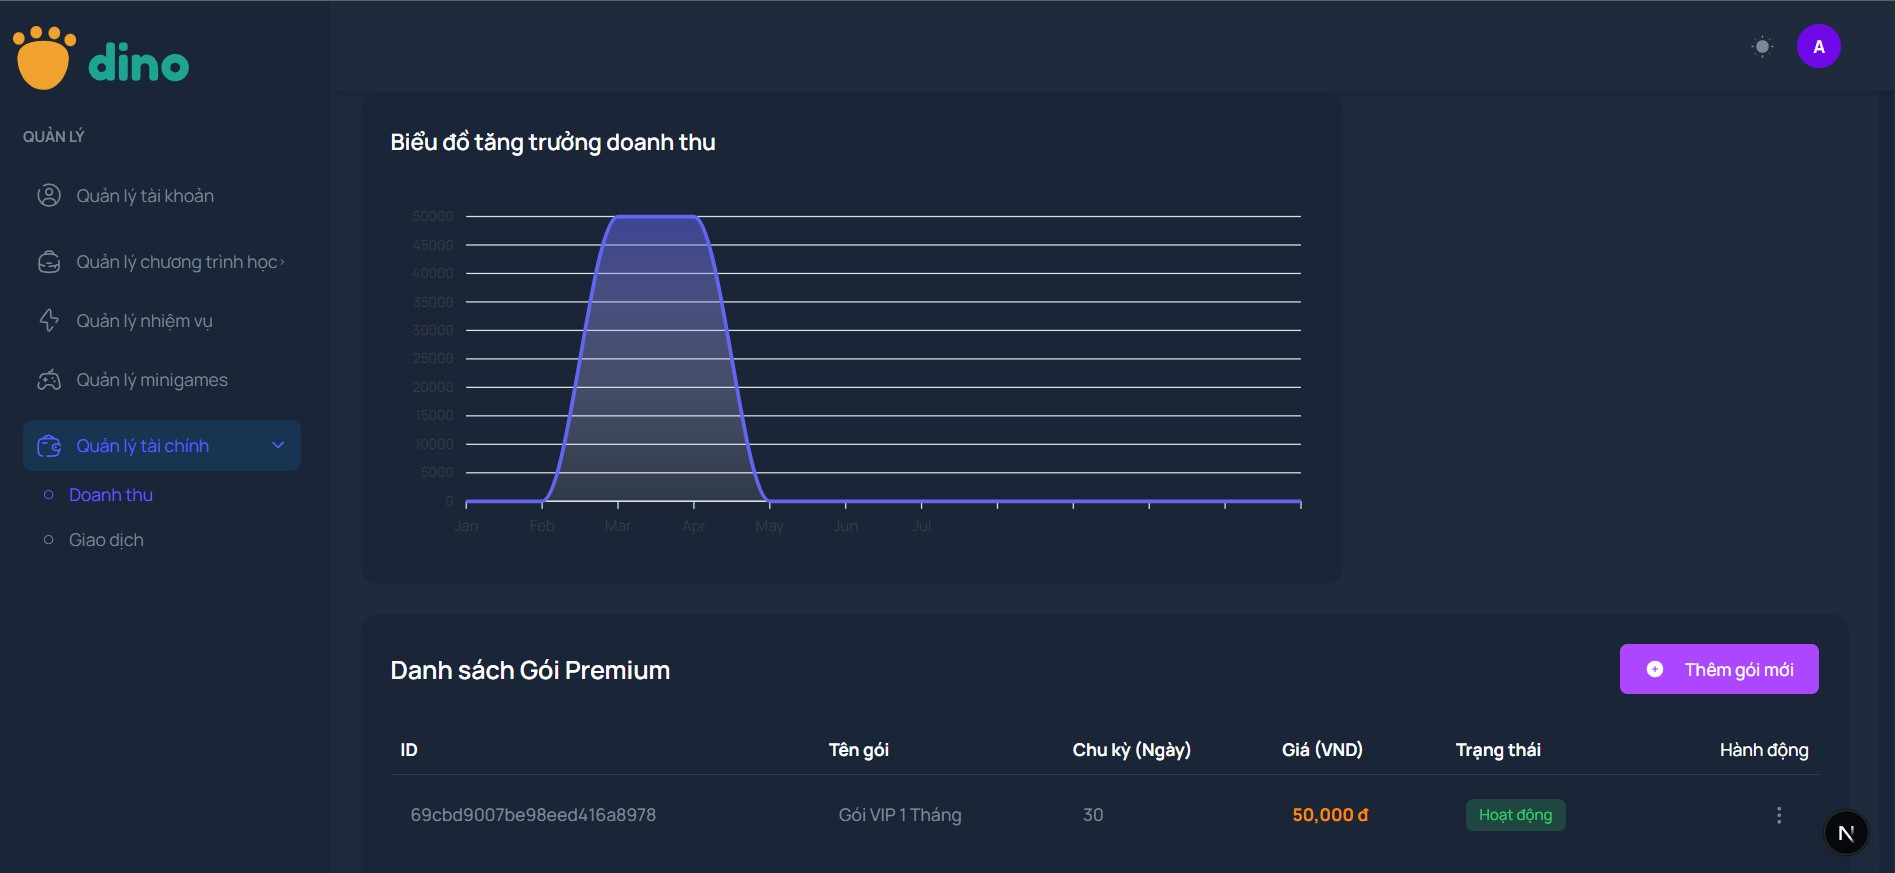
\includegraphics[width=0.9\textwidth]{Image/UI/Admin/Revenue.jpg}
	\vspace{0.6cm}
	\caption{Admin - Quản lý tài chính}
\end{figure}

\subsection{Hệ thống bài tập}
\label{subsec:interact}
Để xây dựng một môi trường học tập toán tư duy hiệu quả, hệ thống bài tập không chỉ dừng lại ở việc kiểm tra kiến thức mà còn phải đóng vai trò là công cụ kích thích sự phát triển trí tuệ. Thiết kế của chúng tôi dựa trên ba trụ cột chính: tính sư phạm, tính tương tác và tính công nghệ.

\subsubsection{Cơ sở thiết kế và chuẩn kiến thức}
Nội dung bài tập được xây dựng dựa trên \textbf{Chương trình Giáo dục phổ thông 2018} của Bộ Giáo dục và Đào tạo Việt Nam \cite{bogddt2018}, tập trung vào 5 mạch kiến thức cốt lõi: Số và phép tính, Hình học và Đo lường, Thống kê và Xác suất. Tuy nhiên, thay vì các bài tập tính toán đơn thuần, chúng tôi tích hợp các phương pháp tư duy từ mô hình giáo dục quốc tế như \textbf{Singapore Math (phương pháp CPA: Concrete-Pictorial-Abstract)} \cite{leong2015concrete} để giúp học sinh Việt Nam dễ dàng chuyển đổi từ tư duy trực quan sang tư duy trừu tượng.

Về mặt học thuật, hệ thống bài tập được tổ chức theo tiến trình phát triển năng lực toán học của học sinh tiểu học từ lớp 1 đến lớp 5, bảo đảm tính kế thừa, đồng tâm và mở rộng dần theo từng khối lớp. Mỗi chủ đề được thiết kế theo ba mức độ \textit{nhận biết -- thông hiểu -- vận dụng}, tương ứng với khả năng nhận diện khái niệm, thực hiện thao tác và giải quyết tình huống thực tiễn; ví dụ từ nhận biết số, phép tính cơ bản ở lớp 1 đến phân số, số thập phân, tỉ số, hình học và toán ứng dụng ở các lớp trên. Cách tổ chức này giúp ngân hàng bài tập vừa bám sát chuẩn đầu ra của chương trình, vừa hỗ trợ hình thành tư duy phân tích, lập luận và giải quyết vấn đề thông qua các ngữ cảnh gần gũi với đời sống học sinh.

\subsubsection{Kiến trúc mô-đun và Công nghệ phát triển}
Hệ thống được thiết kế dựa trên kiến trúc mô-đun linh hoạt, cho phép tách biệt giữa dữ liệu bài toán (Content) và logic tương tác (Logic). 

\begin{itemize}
	\item \textbf{Công cụ phát triển:} Toàn bộ hệ thống tương tác được phát triển trên engine \textbf{Cocos Creator 3.8} \cite{cocoscreator38}. Việc sử dụng hệ thống \textit{Entity Component System (ECS)} của Cocos Creator giúp tối ưu hóa hiệu suất xử lý đồng thời trên cả nền tảng Web và Mobile, đảm bảo các hiệu ứng hoạt hình và phản hồi vật lý mượt mà.
	\item \textbf{Tính mở rộng:} Nhờ vào khả năng quản lý tài nguyên (Asset Management) mạnh mẽ của Cocos 3.8, hệ thống dễ dàng tích hợp thêm các dạng bài tập mới (Drag-and-Drop, Fill-in-the-blank, Logic Matching) mà không làm ảnh hưởng đến cấu trúc tổng thể của ứng dụng.
\end{itemize}

\subsubsection{Giải pháp tương tác và Game hóa (Gamification)}
Khắc phục nhược điểm của các hệ thống cũ tại Việt Nam vốn nặng về lý thuyết, giải pháp của chúng tôi ứng dụng các nguyên lý trong \textbf{Khung lý thuyết Octalysis} \cite{chou2015} để thiết kế hệ thống phần thưởng và nhiệm vụ:
\begin{itemize}
	\item \textbf{Phản hồi tức thì (Instant Feedback):} Sử dụng hệ thống Particle và Animation trong Cocos Creator để tạo ra các hiệu ứng khích lệ khi học sinh giải đúng, giúp duy trì trạng thái "Flow" (luồng hứng thú) trong quá trình học.
	\item \textbf{Tương tác đa chạm:} Tận dụng tối đa bộ lọc sự kiện (Input Events) của Cocos để tạo ra các bài tập kéo thả vật thể, xoay hình học không gian, giúp học sinh tiểu học phát triển tư duy hình khối một cách trực quan nhất.
\end{itemize}

\subsubsection{Các dạng toán}

\subsubsubsection{Trắc nghiệm (Multiple Choice)}
Dạng bài tập trắc nghiệm cho phép người học lựa chọn một đáp án đúng trong bốn đáp án được cung cấp sẵn. Sau khi chọn đáp án, hệ thống sẽ phản hồi trực quan bằng hiệu ứng nhấp nháy hoặc đổi màu để giúp học sinh nhận biết kết quả ngay lập tức. Dạng bài này thường được sử dụng để luyện tập các phép tính cơ bản, nhận diện hình học, so sánh số hoặc các câu hỏi lý thuyết đơn giản phù hợp với học sinh tiểu học.

\begin{figure}[H]
	\centering
	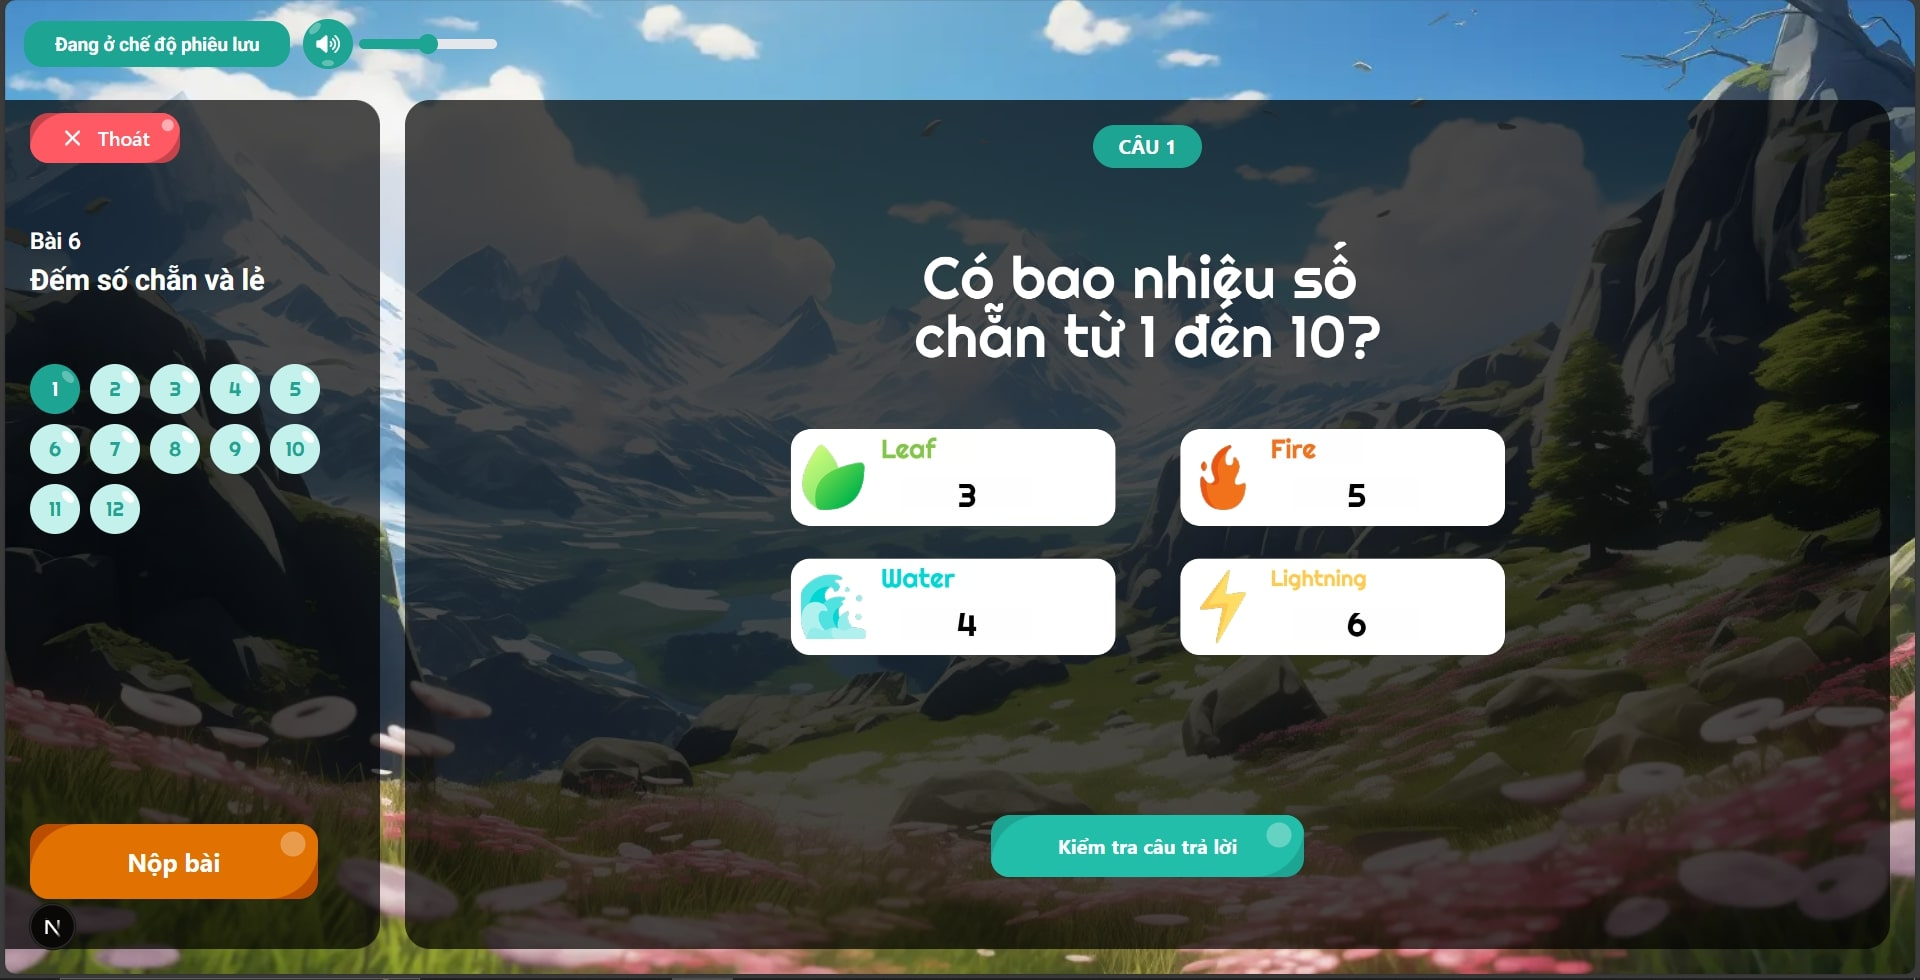
\includegraphics[width=0.9\textwidth]{Image/UI/Exercises/MultiChoice.jpg}
	\caption{Dạng bài trắc nghiệm}
	\label{fig:multiple-choice}
\end{figure}

\subsubsubsection{Ghép cặp (Matching)}
Trong dạng bài ghép cặp, người học thực hiện thao tác kéo thả để nối các đối tượng tương ứng với nhau, ví dụ như phép tính với kết quả tương ứng. Khi ghép đúng, các đối tượng sẽ đổi màu hoặc xuất hiện hiệu ứng phản hồi nhằm tăng tính trực quan và tạo cảm giác hứng thú trong quá trình học tập.

\begin{figure}[H]
	\centeringMô 
	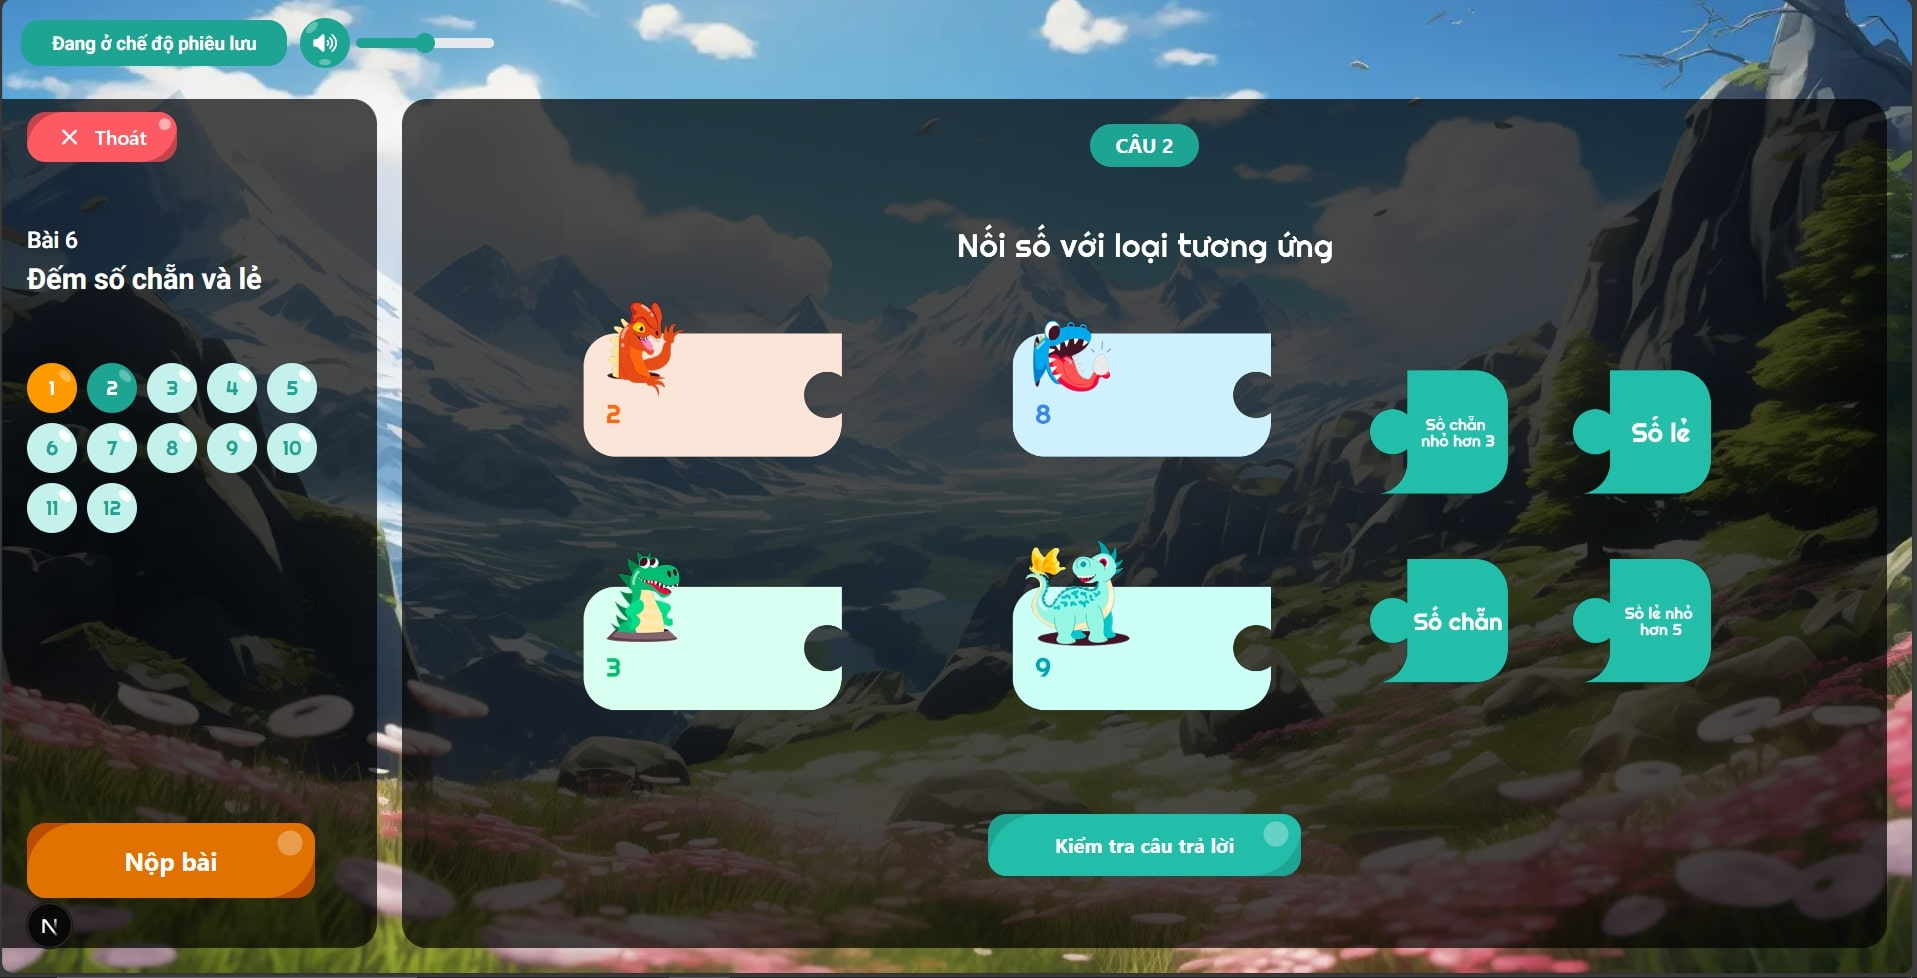
\includegraphics[width=0.9\textwidth]{Image/UI/Exercises/Matching.jpg}
	\caption{Dạng bài ghép cặp}
	\label{fig:matching}
\end{figure}

\subsubsubsection{Điền số (Fill in the Blanks)}
Dạng bài điền số yêu cầu học sinh nhập giá trị thích hợp vào các ô trống trong biểu thức hoặc câu hỏi toán học. Một bài có thể chứa tối đa ba ô trống và hệ thống sẽ chấm điểm độc lập cho từng phần nhằm hỗ trợ đánh giá chính xác hơn. Dạng bài này giúp rèn luyện khả năng tính toán và tư duy từng bước của người học.

\begin{figure}[H]
	\centering
	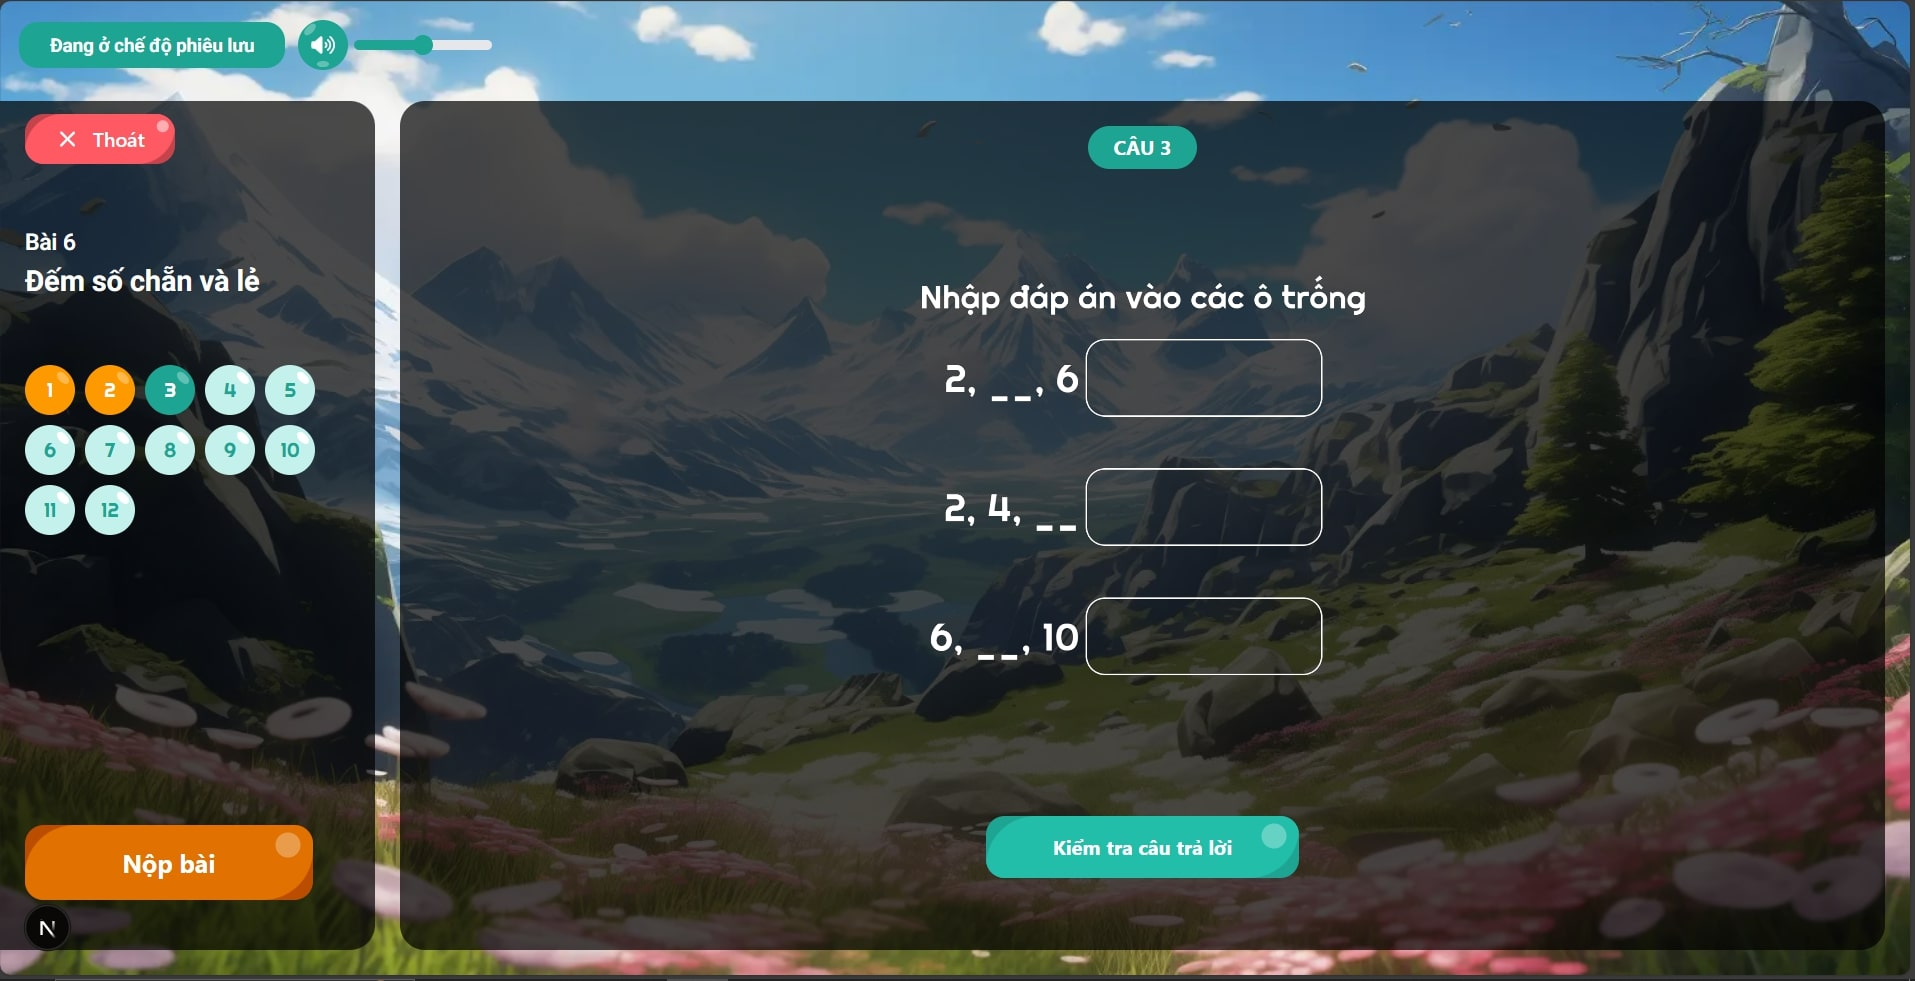
\includegraphics[width=0.9\textwidth]{Image/UI/Exercises/Fill.jpg}
	\caption{Dạng bài điền số}
	\label{fig:fill}
\end{figure}

\subsubsubsection{Kéo thả (Drag and Drop)}
Ở dạng bài này, người học sẽ kéo các con số hoặc ký hiệu toán học vào đúng vị trí còn thiếu trong biểu thức. Nếu thả sai vị trí, hệ thống sẽ tự động đưa đối tượng trở về vị trí ban đầu để người học thử lại. Cơ chế tương tác trực tiếp giúp học sinh dễ dàng tiếp cận và ghi nhớ các phép tính cơ bản.

\begin{figure}[H]
	\centering
	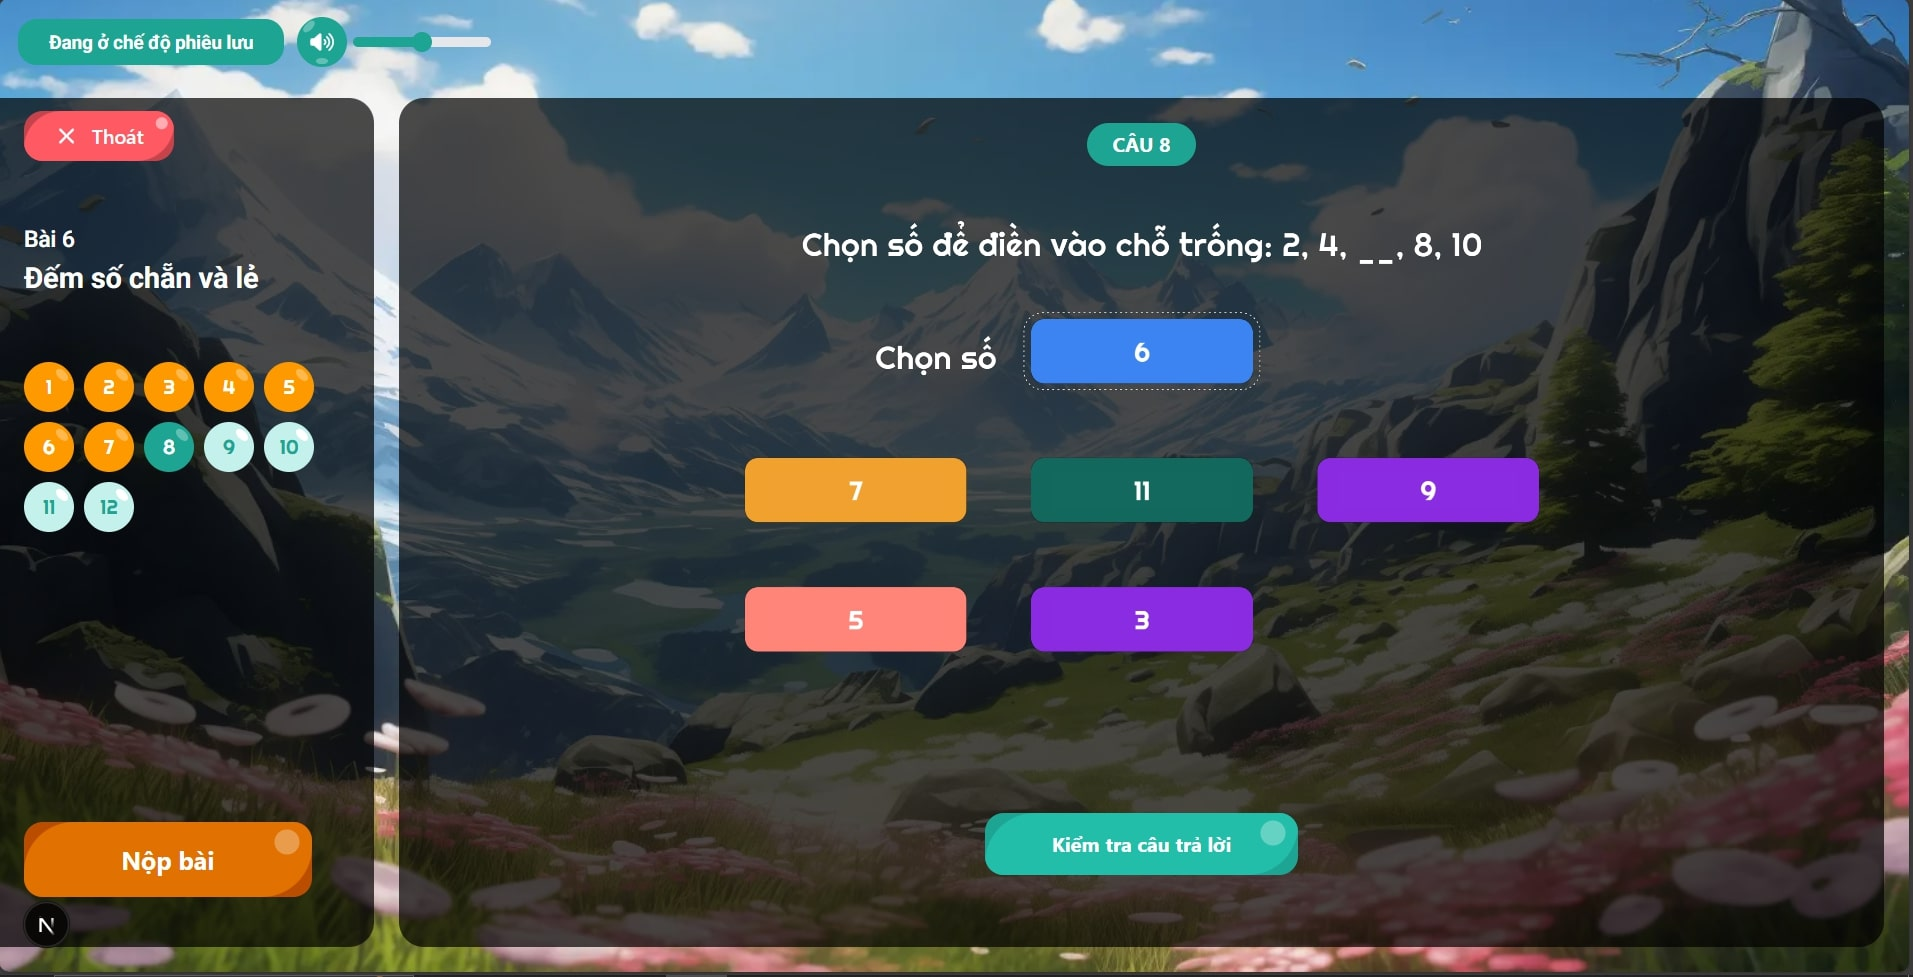
\includegraphics[width=0.9\textwidth]{Image/UI/Exercises/Drag.jpg}
	\caption{Dạng bài kéo thả}
	\label{fig:drag}
\end{figure}

\subsubsubsection{Phân loại chẵn/lẻ (Grouping)}
Dạng bài phân loại yêu cầu học sinh lựa chọn chế độ phân loại trước khi bắt đầu làm bài, trong đó số chẵn được biểu diễn bằng màu xanh và số lẻ được biểu diễn bằng màu hồng. Sau khi chọn chế độ, người học sẽ click trực tiếp vào từng con số để tô màu tương ứng, tương tự như một trò chơi tô màu tương tác. Hệ thống chỉ kiểm tra kết quả sau khi hoàn thành toàn bộ thao tác, giúp học sinh tập trung vào quá trình quan sát, suy luận và tự đánh giá trước khi nộp đáp án.

\begin{figure}[H]
	\centering
	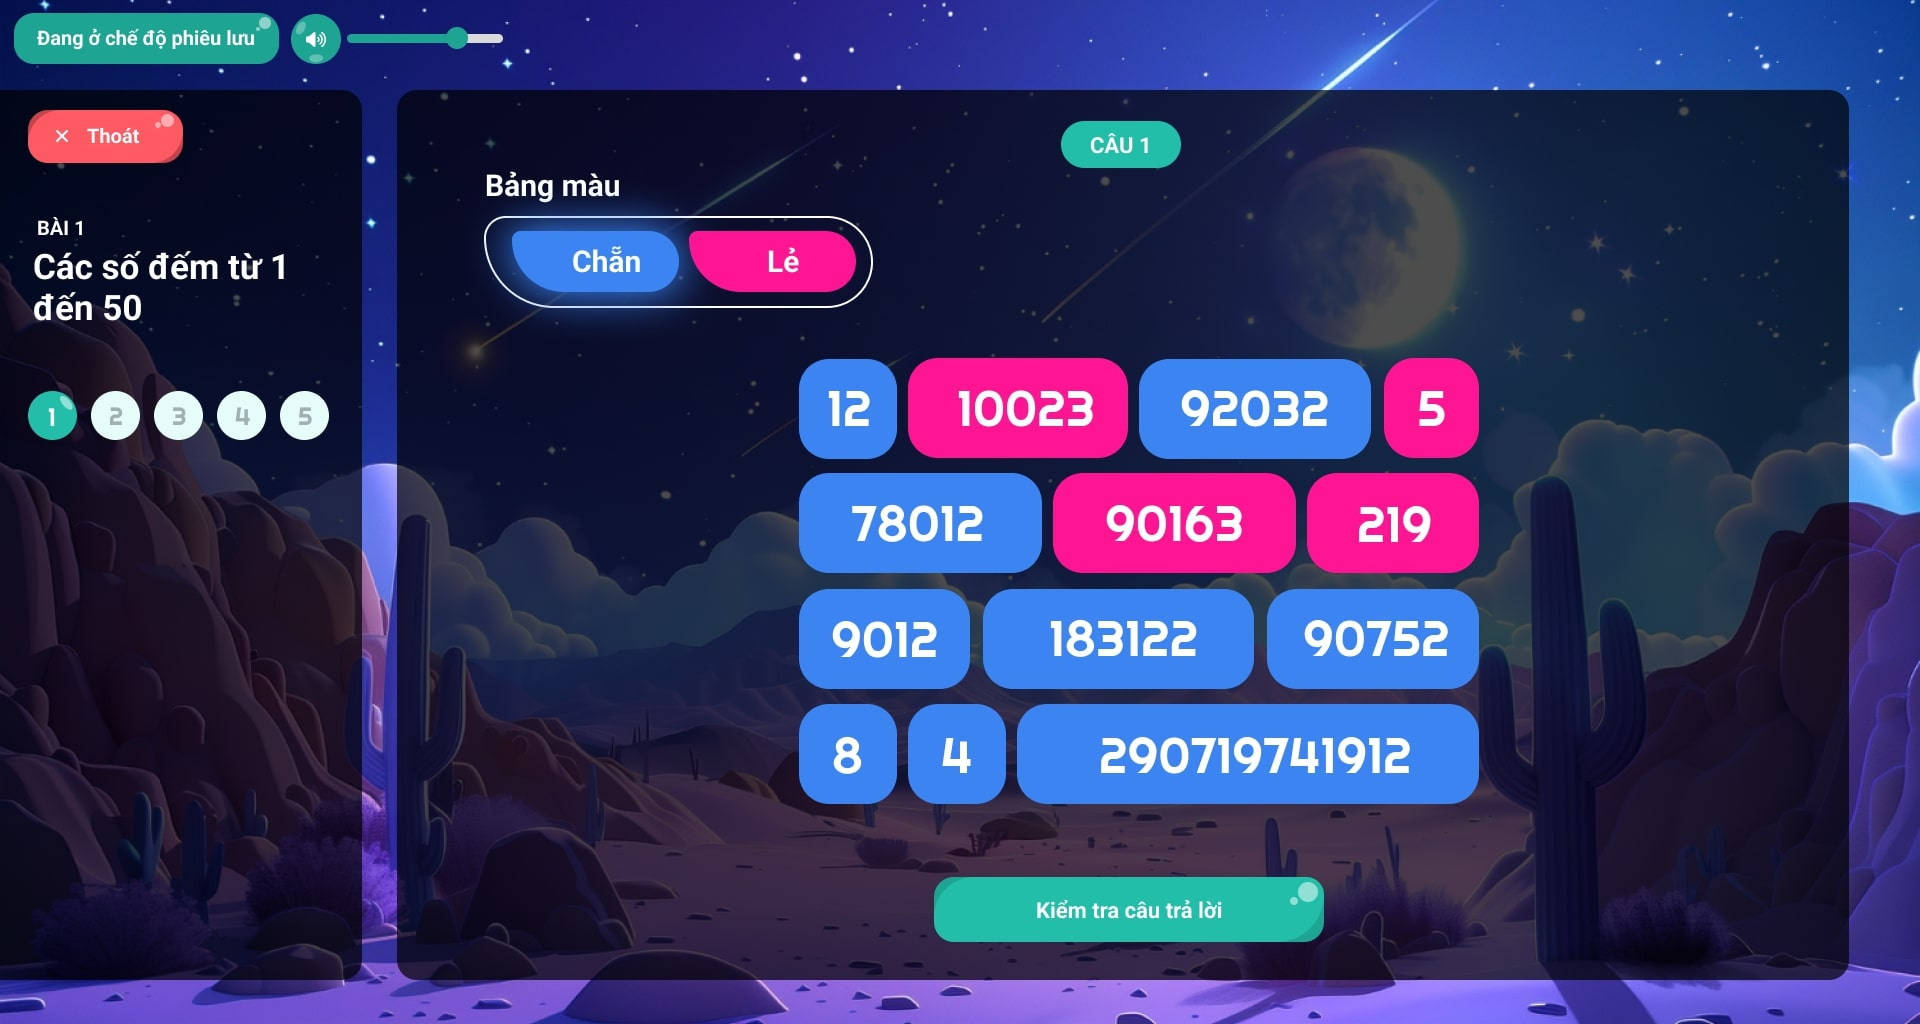
\includegraphics[width=0.9\textwidth]{Image/UI/Exercises/Grouping.jpg}
	\caption{Dạng bài phân loại}
	\label{fig:grouping}
\end{figure}

\subsubsubsection{Đúng/Sai (True/False)}
Dạng bài đúng/sai cung cấp cho người học một mệnh đề hoặc phép tính và yêu cầu lựa chọn “Đúng” hoặc “Sai”. Hệ thống chỉ cho phép một lựa chọn duy nhất nhằm đảm bảo tính rõ ràng trong câu trả lời. Đây là dạng bài đơn giản nhưng hiệu quả trong việc kiểm tra khả năng nhận biết nhanh và tư duy logic của học sinh.

\begin{figure}[H]
	\centering
	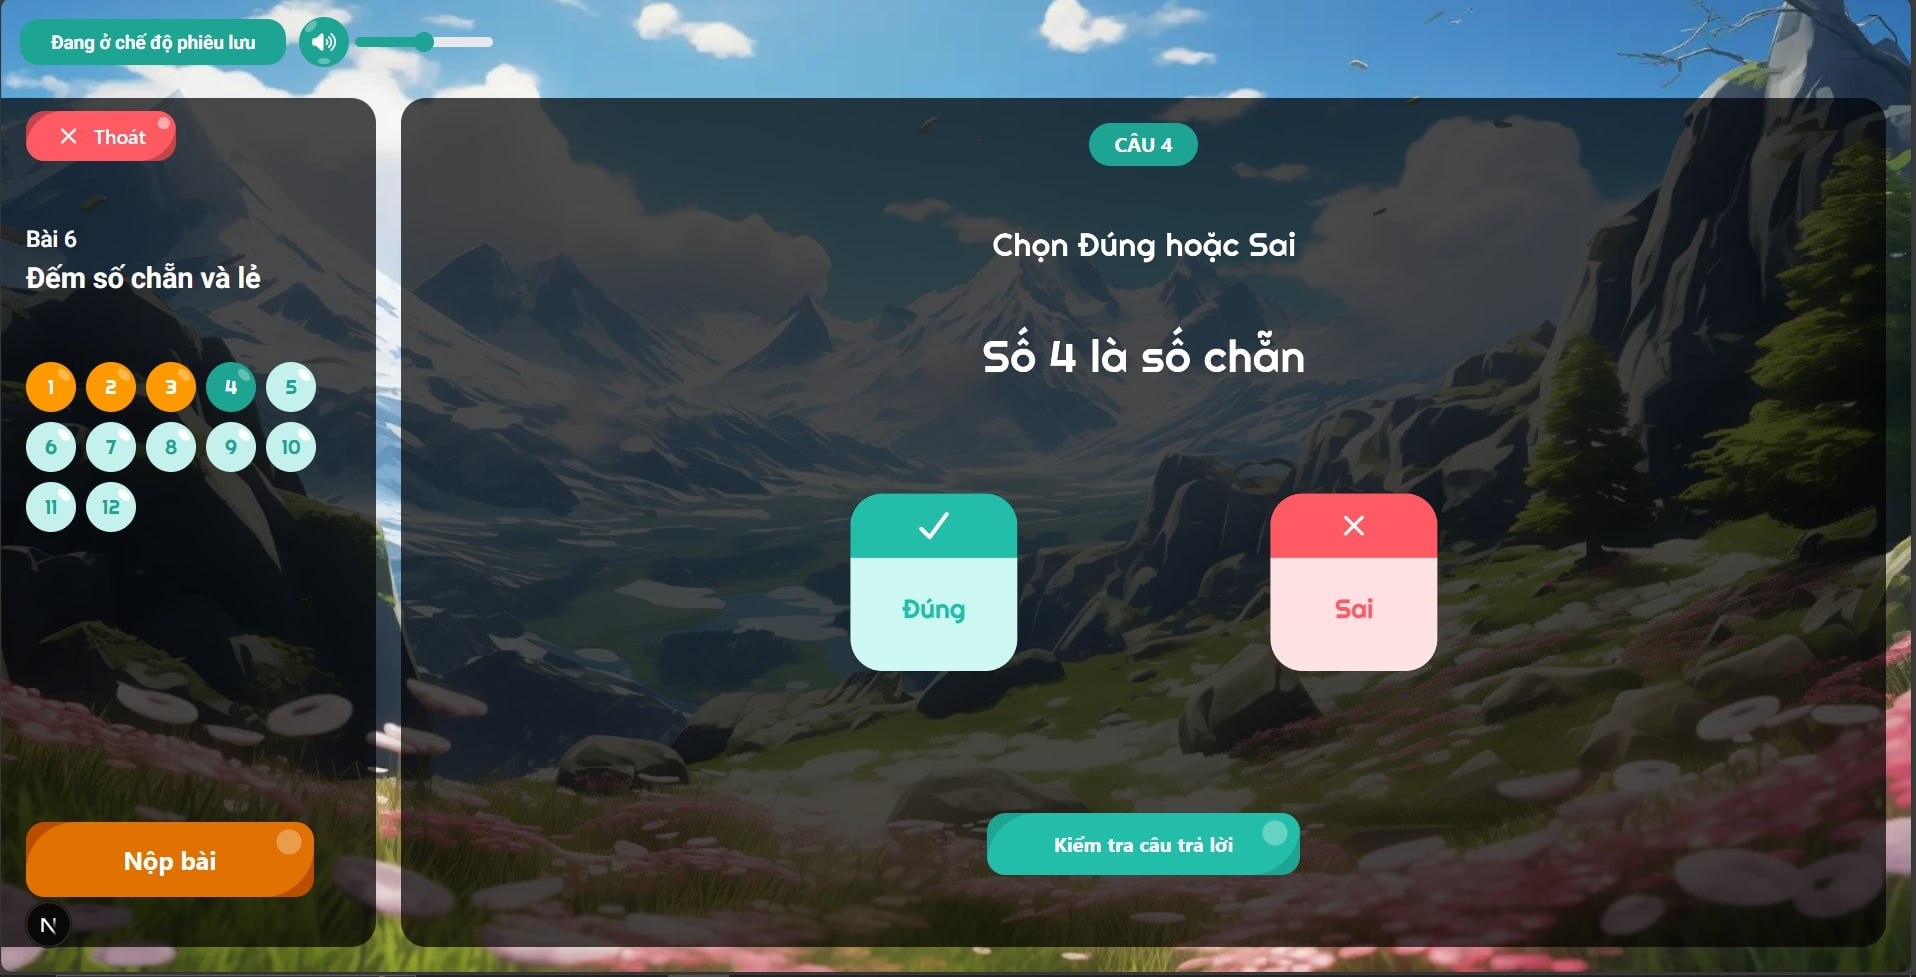
\includegraphics[width=0.9\textwidth]{Image/UI/Exercises/TrueFalse.jpg}
	\caption{Dạng bài đúng/sai}
	\label{fig:truefalse}
\end{figure}

\subsubsubsection{Tổ hợp burger (Burger)}
Dạng bài tổ hợp burger giúp học sinh làm quen với tư duy tổ hợp và lựa chọn thành phần theo yêu cầu đề bài. Hệ thống cung cấp bốn loại nguyên liệu gồm cà chua, thịt, phô mai và rau. Dựa trên yêu cầu của bài toán, người học cần lựa chọn và sắp xếp đúng các nguyên liệu để tạo ra chiếc burger phù hợp. Một bài toán có thể có nhiều cách tạo burger khác nhau miễn đáp ứng đúng yêu cầu về thành phần.

\begin{figure}[H]
	\centering
	
\includegraphics[width=0.9\textwidth]{Image/UI/Exercises/Burger.jpg}
	\caption{Dạng bài tổ hợp burger}
	\label{fig:burger}
\end{figure}

\subsubsubsection{Xe buýt (Bus)}
Dạng bài xe buýt được xây dựng nhằm giúp học sinh hiểu rõ giá trị hàng đơn vị, hàng chục và hàng trăm. Hệ thống cung cấp ba loại hộp tương ứng với giá trị 1, 10 và 100. Theo yêu cầu bài toán, học sinh cần lựa chọn các hộp sao cho tổng giá trị đúng với số lượng cần vận chuyển. Ví dụ, để vận chuyển 100 linh kiện, học sinh có thể chọn một hộp 100 hoặc mười hộp 10. Khi chọn hộp, các hộp sẽ bay trực tiếp lên xe buýt tạo nên trải nghiệm học tập sinh động và trực quan.

\begin{figure}[H]
	\centering
	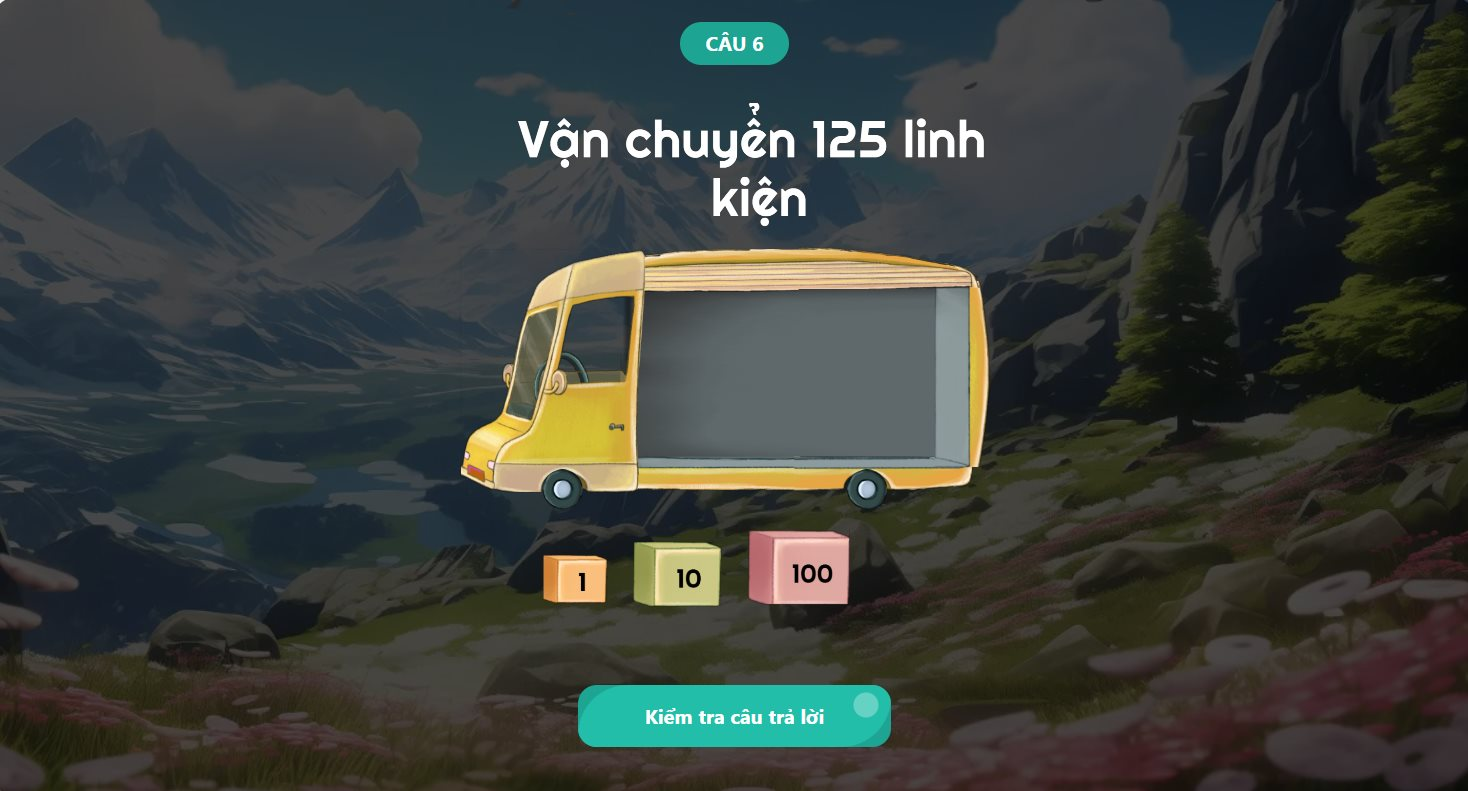
\includegraphics[width=0.9\textwidth]{Image/UI/Exercises/Bus.jpg}
	\caption{Dạng bài xe buýt}
	\label{fig:bus}
\end{figure}

\subsubsubsection{Bắt chim (Catch Bird)}
Trong dạng bài bắt chim, trên cây sẽ có một số lượng chim ban đầu và người học cần click vào các chú chim để chúng bay vào lồng. Số lượng chim trong lồng sẽ đại diện cho kết quả của bài toán. Nhờ cơ chế biểu diễn trực quan này, hệ thống có thể mở rộng thành nhiều dạng câu hỏi khác nhau.

\begin{figure}[H]
	\centering
	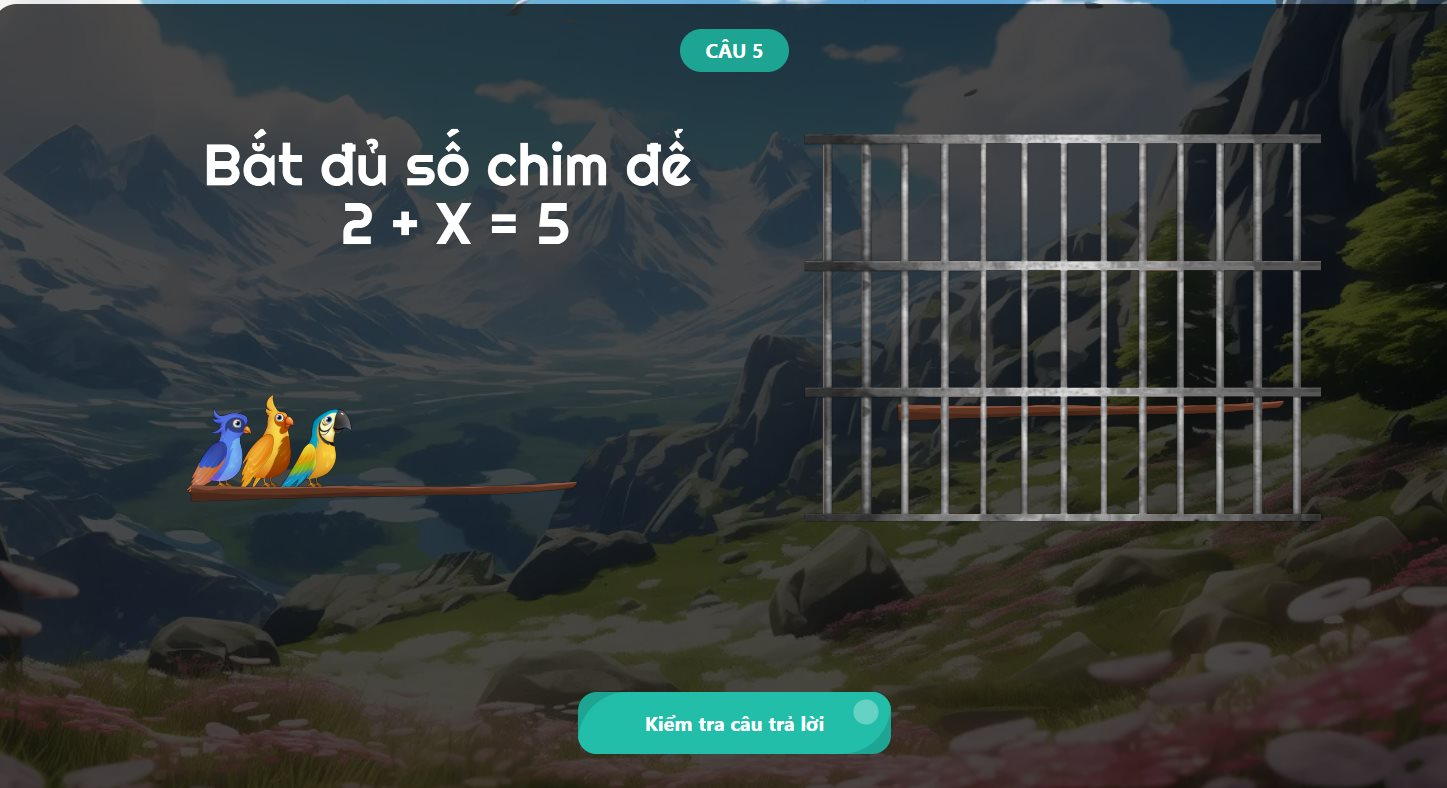
\includegraphics[width=0.9\textwidth]{Image/UI/Exercises/CatchBird.jpg}
	\caption{Dạng bài bắt chim}
	\label{fig:catchbird}
\end{figure}

\subsubsubsection{Đồng hồ (Clock)}
Dạng bài đồng hồ giúp học sinh học cách xem giờ thông qua đồng hồ kim 12 giờ. Người học cần xoay kim đồng hồ đến đúng thời gian được yêu cầu. Điểm đặc biệt của dạng bài này là hệ thống có thêm khung cửa sổ mô phỏng thời gian ngày và đêm. Ví dụ, khi chỉnh đến 12 giờ trưa, khung cửa sổ sẽ hiển thị mặt trời và bầu trời sáng; ngược lại khi chỉnh đến 12 giờ đêm, cửa sổ sẽ hiển thị bầu trời tối cùng mặt trăng. Điều này giúp học sinh phân biệt rõ khái niệm hệ thống giờ 12 giờ và 24 giờ một cách trực quan và sinh động hơn

\begin{figure}[H]
	\centering
	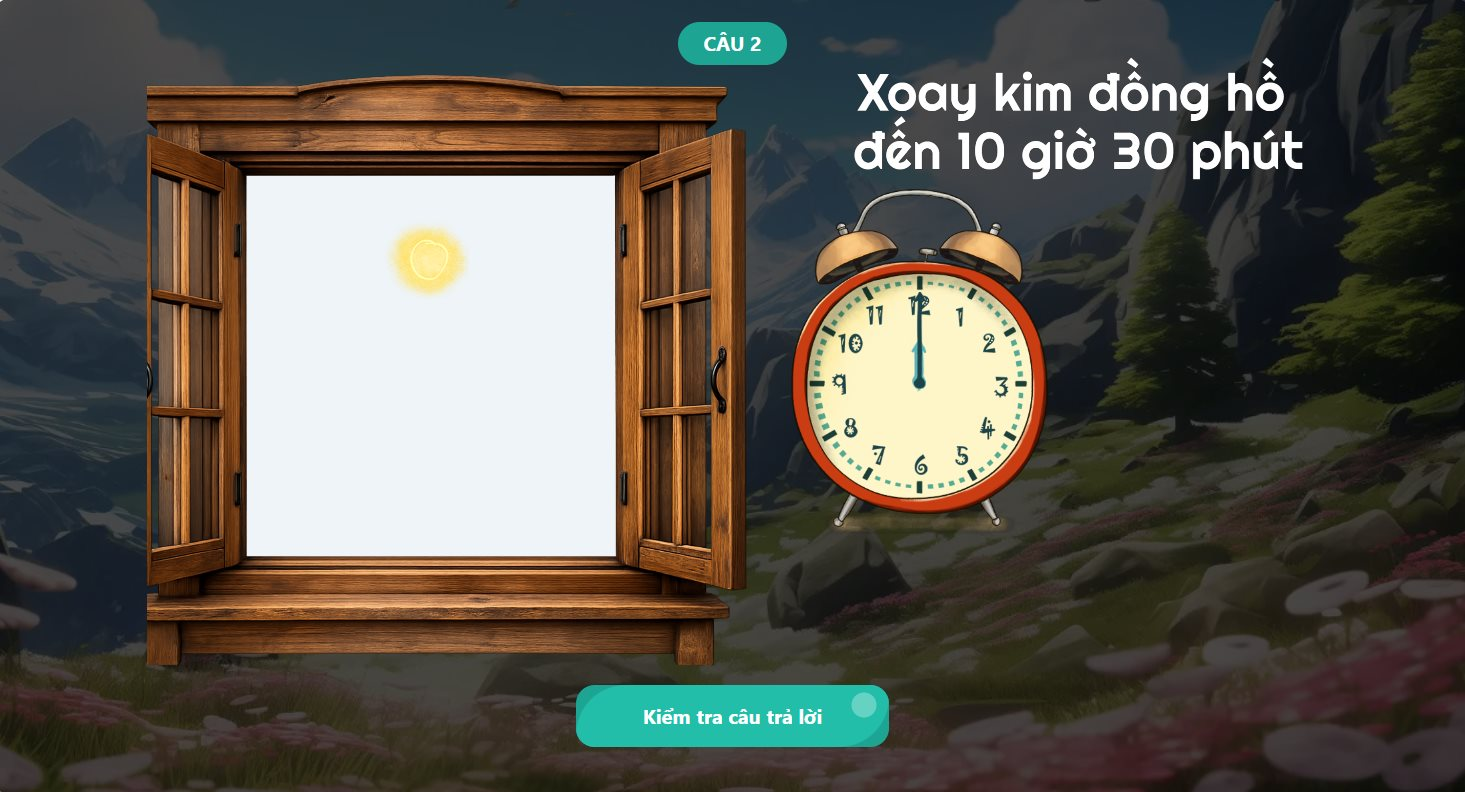
\includegraphics[width=0.9\textwidth]{Image/UI/Exercises/Clock.jpg}
	\caption{Dạng bài đồng hồ}
	\label{fig:clock}
\end{figure}

\subsubsubsection{Đổi tiền xu (Coin)}
Dạng bài đổi tiền xu hỗ trợ học sinh làm quen với giá trị tiền tệ thông qua cơ chế đổi tiền trực quan. Hệ thống cung cấp ba loại đồng xu có giá trị 1 đồng, 10 đồng và 100 đồng cùng với một máy đổi tiền. Khi đưa một đồng xu vào máy, hệ thống sẽ tự động đổi sang các đồng xu có giá trị nhỏ hơn, ví dụ một đồng 100 sẽ đổi thành mười đồng 10. Người học cần vận dụng cơ chế đổi tiền để tạo đúng số tiền theo yêu cầu của bài toán.

\begin{figure}[H]
	\centering
	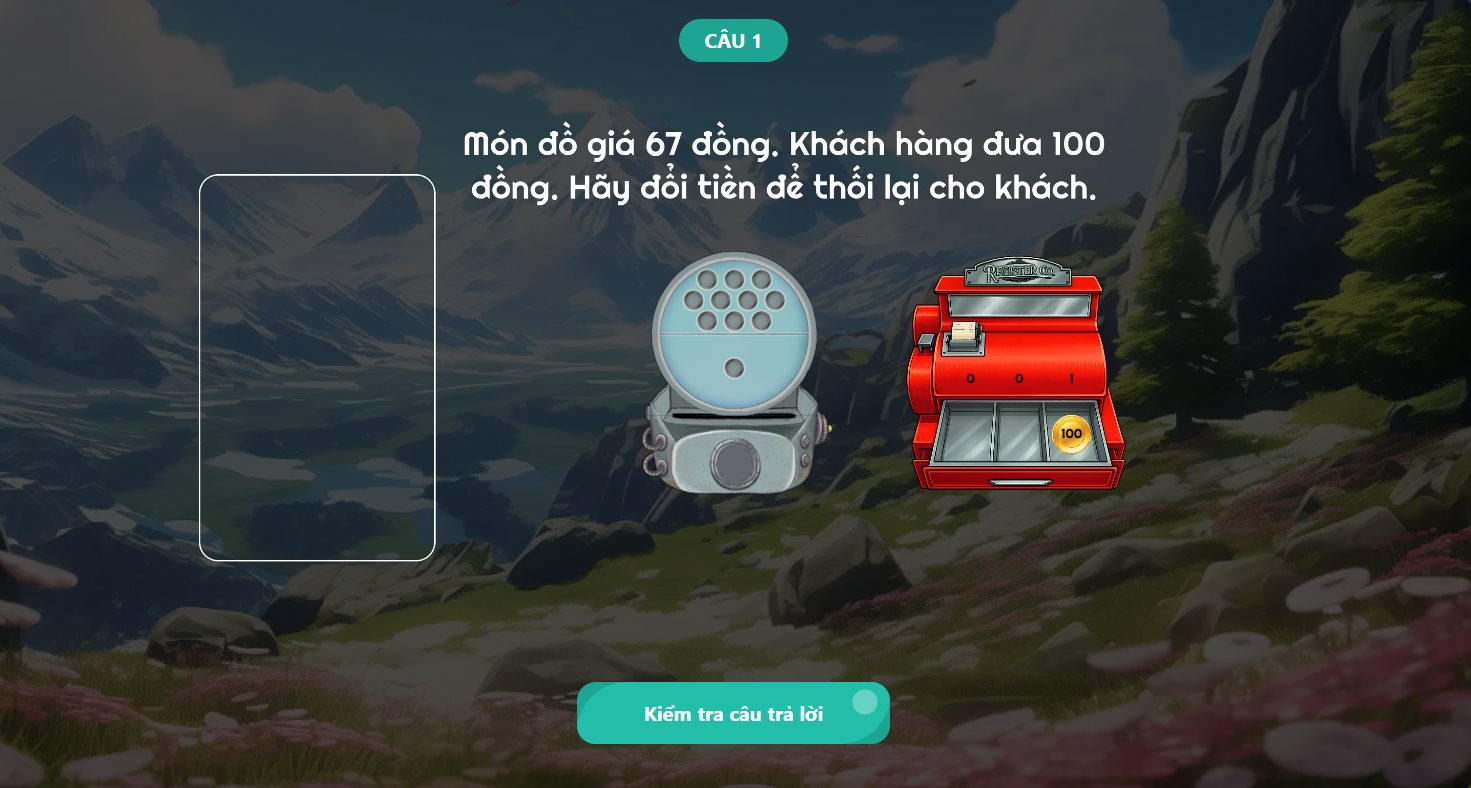
\includegraphics[width=0.9\textwidth]{Image/UI/Exercises/Coin.jpg}
	\caption{Dạng bài đổi tiền xu}
	\label{fig:coin}
\end{figure}

\subsubsubsection{Viên bi (Gumball)}
Dạng bài viên bi được thiết kế nhằm hỗ trợ học sinh luyện tập kỹ năng đếm và so sánh số lượng. Ban đầu hệ thống cung cấp một số lượng bi xanh và bi cam nhất định. Khi người học chọn một chiếc lọ, chiếc lọ sẽ di chuyển vào máy để hứng bi rơi xuống. Mỗi lần máy sẽ thả 10 viên bi và mỗi lọ chứa đúng 10 viên. Học sinh cần quan sát số lọ đã đầy cùng số viên còn lại để trả lời các câu hỏi so sánh như màu nào nhiều hơn hoặc ít hơn.

\begin{figure}[H]
	\centering
	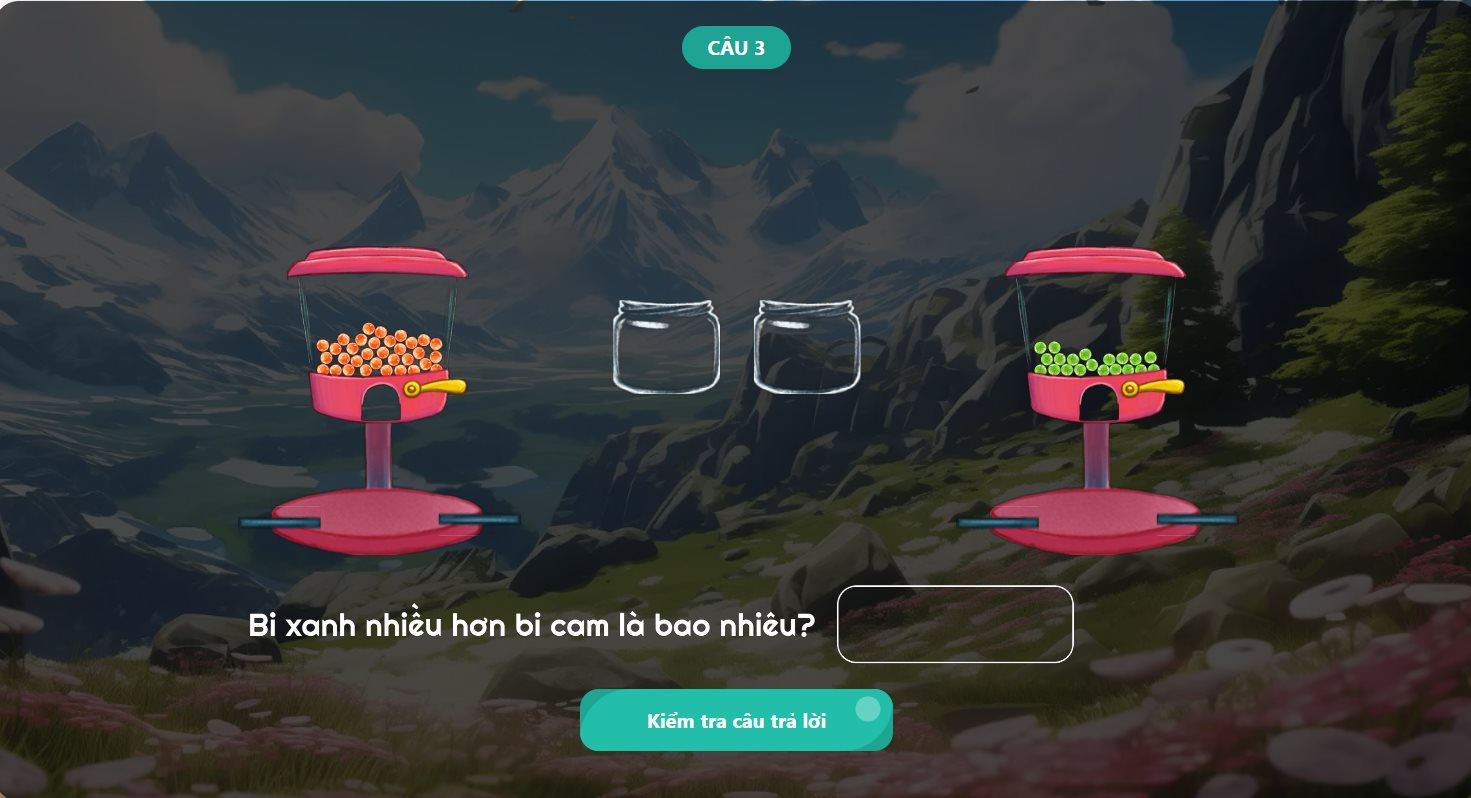
\includegraphics[width=0.9\textwidth]{Image/UI/Exercises/Gumball.jpg}
	\caption{Dạng bài viên bi}
	\label{fig:gumball}
\end{figure}

\subsubsubsection{Cân thủ công (Manual Scale)}
Dạng bài cân thủ công sử dụng mô hình cân đòn nhằm giúp học sinh làm quen với các khái niệm lớn hơn, bé hơn và bằng nhau. Người học sẽ kéo các bát hạt lên hai bên cân theo yêu cầu của đề bài. Dựa vào độ nghiêng của cân sang trái hoặc phải, học sinh có thể trực quan nhận biết mối quan hệ giữa hai giá trị.

\begin{figure}[H]
	\centering
	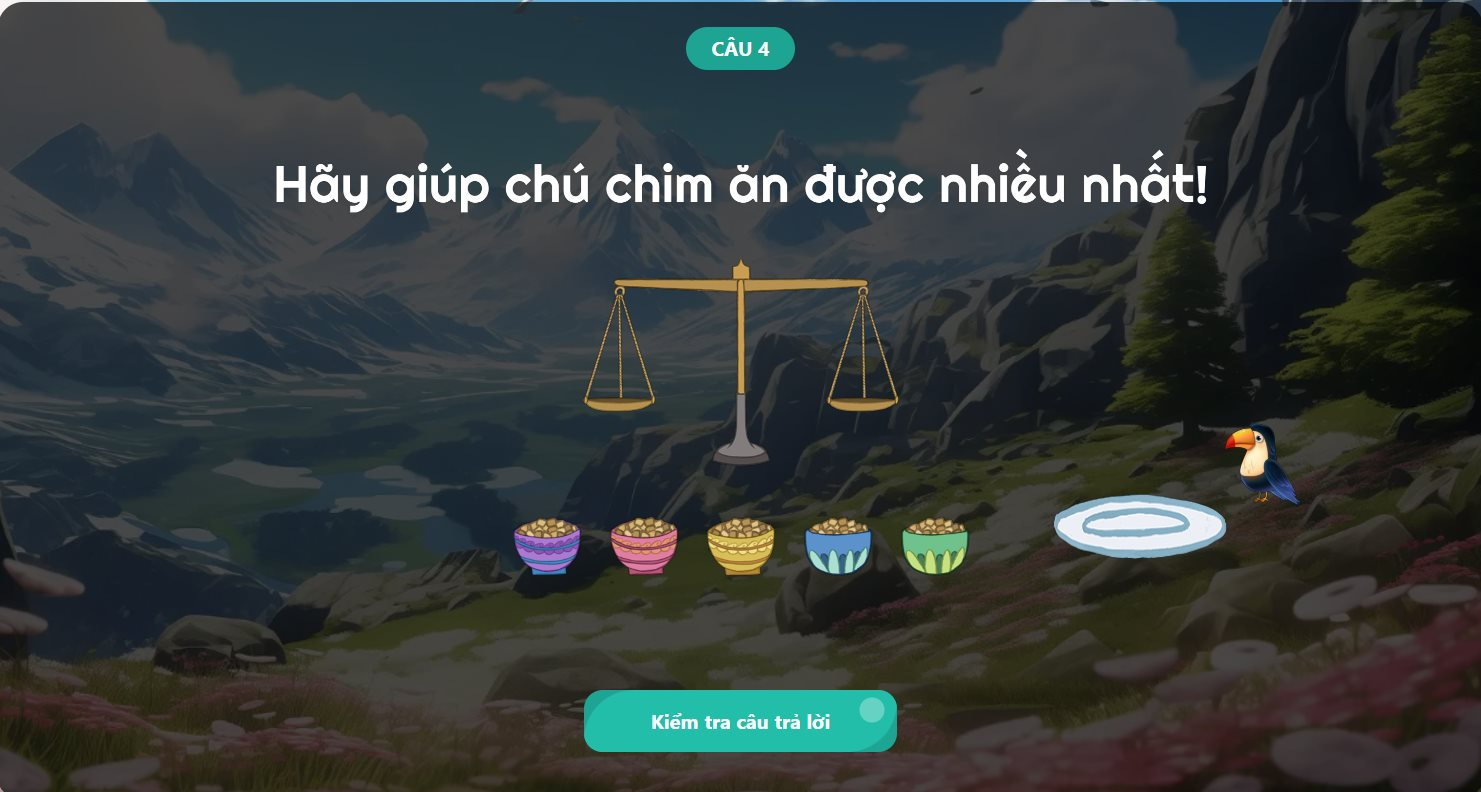
\includegraphics[width=0.9\textwidth]{Image/UI/Exercises/ManualScale.jpg}
	\caption{Dạng bài cân thủ công}
	\label{fig:manual-scale}
\end{figure}

\subsubsubsection{Chia pizza (Pizza)}
Dạng bài chia pizza giúp học sinh bước đầu làm quen với phân số thông qua việc chia chiếc pizza thành nhiều phần bằng nhau. Mỗi lát pizza sẽ có một loại topping khác nhau và bài toán sẽ yêu cầu người học tạo đúng số lượng lát tương ứng với từng loại. Dạng bài này giúp học sinh hình dung trực quan khái niệm phân số trong toán học.

\begin{figure}[H]
	\centering
	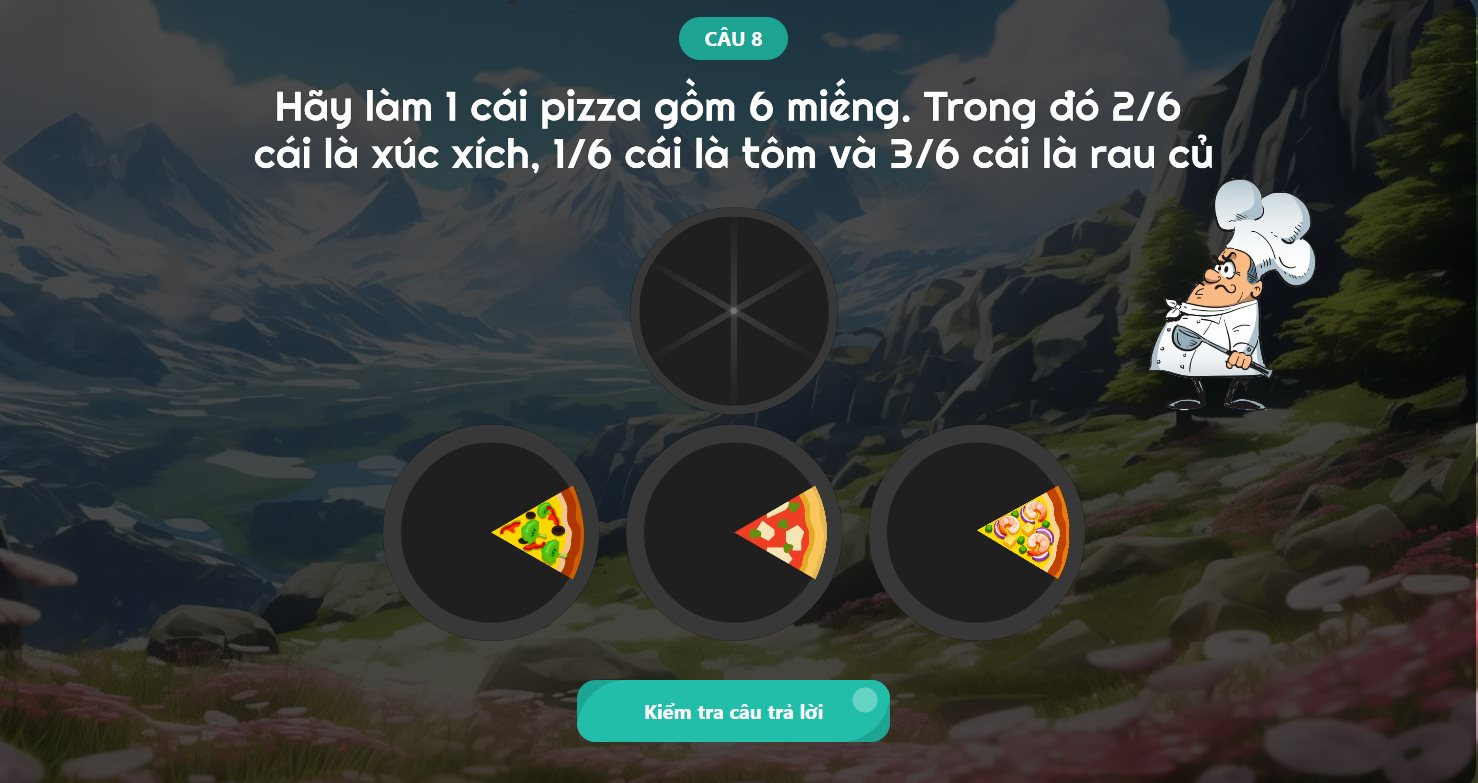
\includegraphics[width=0.9\textwidth]{Image/UI/Exercises/Pizza.jpg}
	\caption{Dạng bài chia pizza}
	\label{fig:pizza}
\end{figure}

\subsubsubsection{Thả chim (Release Bird)}
Dạng bài thả chim có cơ chế tương tự bài trắc nghiệm nhưng được thiết kế với phong cách tương tác sinh động hơn dành cho học sinh lớp nhỏ. Mỗi đáp án được biểu diễn bằng một chiếc lồng chim, phía dưới có bảng hiển thị nội dung đáp án tương ứng. Khi người học chọn đáp án, chiếc lồng sẽ rơi xuống và mở ra để chú chim bay đi, tạo cảm giác vui nhộn và tăng hứng thú học tập.

\begin{figure}[H]
	\centering
	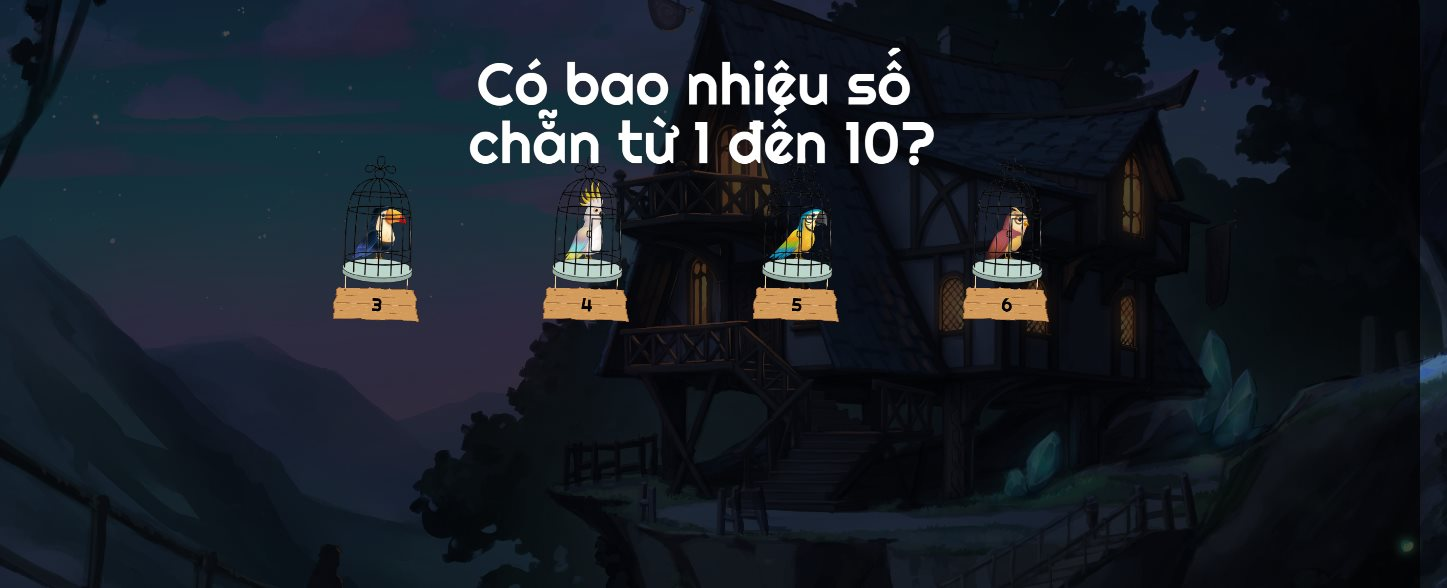
\includegraphics[width=0.9\textwidth]{Image/UI/Exercises/RealeaseBirt.jpg}
	\caption{Dạng bài thả chim}
	\label{fig:release-bird}
\end{figure}

\subsubsubsection{Cân điện tử (Scale)}
Dạng bài cân điện tử yêu cầu học sinh lựa chọn các quả tạ có giá trị khác nhau để đạt đúng khối lượng mục tiêu được đề bài đưa ra. Người học sẽ kéo các quả tạ lên bàn cân và hệ thống sẽ tự động tính tổng khối lượng hiện tại. Một bài toán có thể tồn tại nhiều cách chọn tạ khác nhau miễn tổng khối lượng đạt đúng yêu cầu.

\begin{figure}[H]
	\centering
	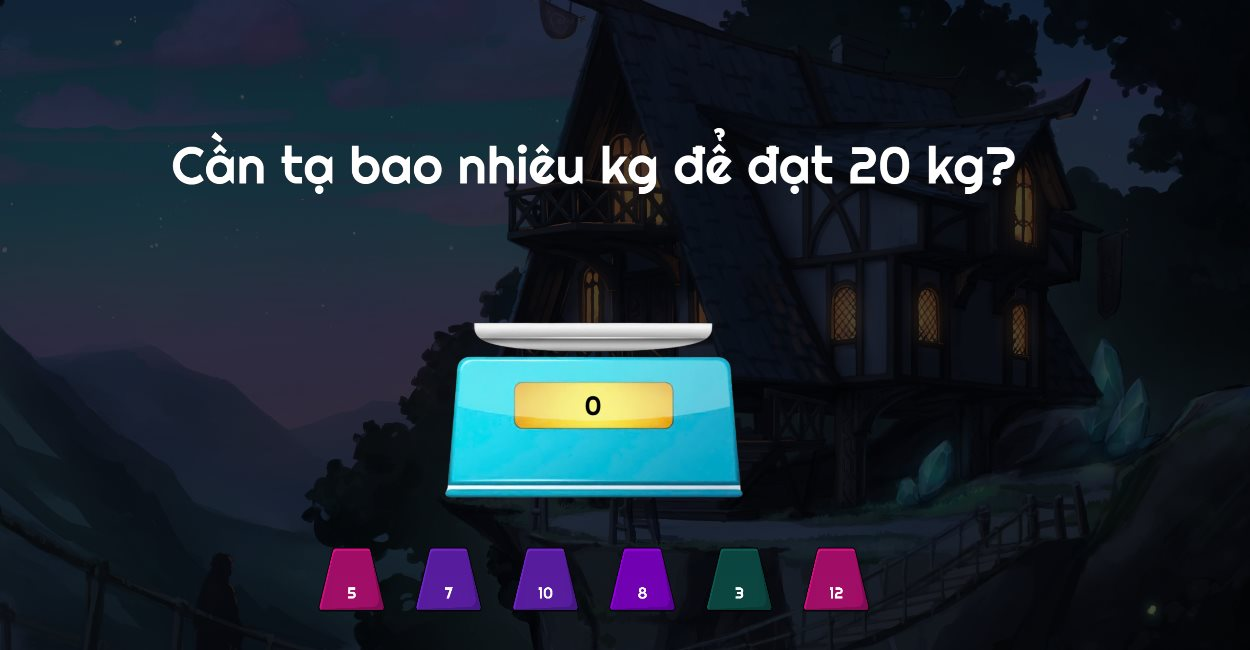
\includegraphics[width=0.9\textwidth]{Image/UI/Exercises/Scale.jpg}
	\caption{Dạng bài cân điện tử}
	\label{fig:scale}
\end{figure}

\subsubsubsection{Tưới cây (Tree)}
Dạng bài tưới cây gồm năm giai đoạn phát triển của cây tương ứng với năm câu hỏi liên tiếp. Mỗi khi trả lời đúng, mây sẽ xuất hiện và tạo mưa giúp cây phát triển sang giai đoạn tiếp theo. Nếu trả lời sai, cây sẽ quay trở lại trạng thái trước đó. Đáp án của mỗi câu hỏi được biểu diễn bằng số lần nhấn nút tương tác. Ví dụ, với bài toán \(2 + X = 5\), học sinh cần nhấn nút ba lần để tạo ra đáp án đúng.

\begin{figure}[H]
	\centering
	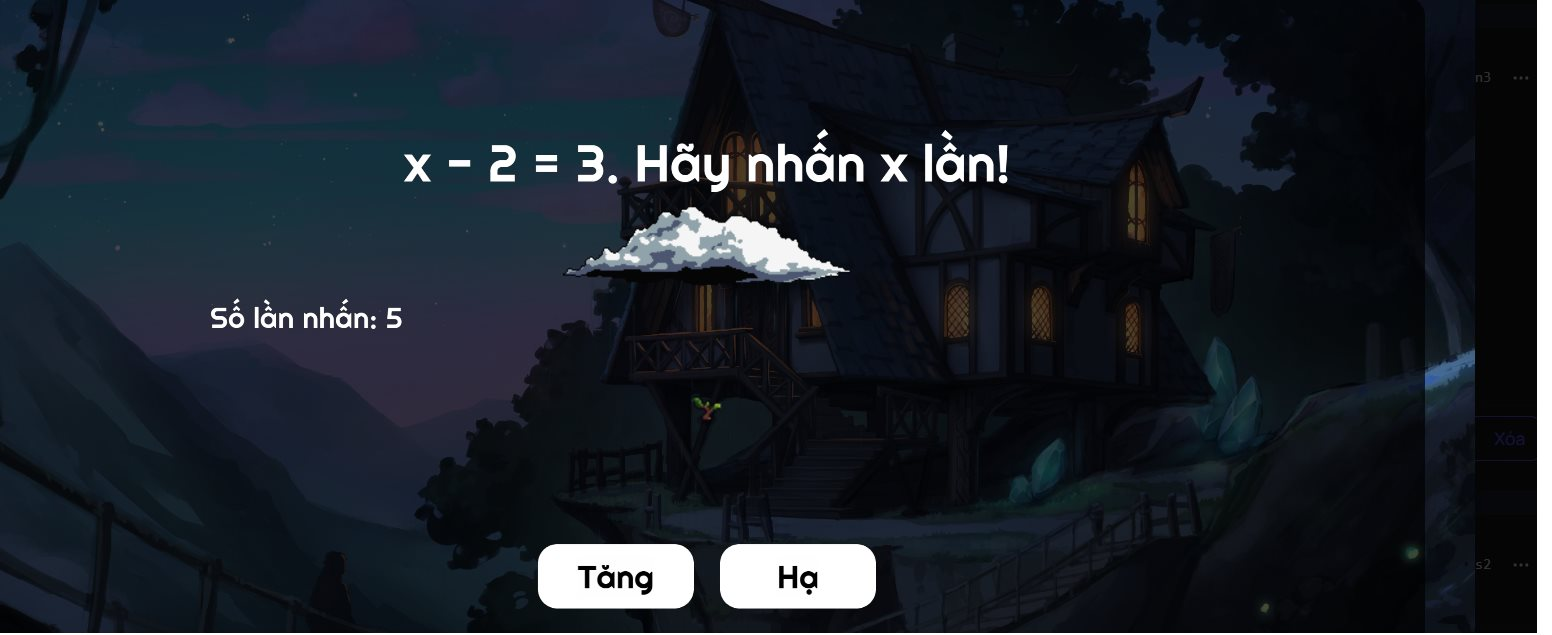
\includegraphics[width=0.9\textwidth]{Image/UI/Exercises/Tree.jpg}
	\caption{Dạng bài tưới cây}
	\label{fig:tree}
\end{figure}

\subsubsubsection{Vẽ hình (Geo)}
Dạng bài vẽ hình được xây dựng theo cơ chế tương tự geoboard. Người học có thể chọn các điểm cố định trên bảng và kéo nối để tạo thành các hình học khác nhau. Hệ thống hỗ trợ nhiều cách vẽ khác nhau cho cùng một đáp án, giúp tăng tính sáng tạo và khả năng tư duy hình học của học sinh.

\begin{figure}[H]
	\centering
	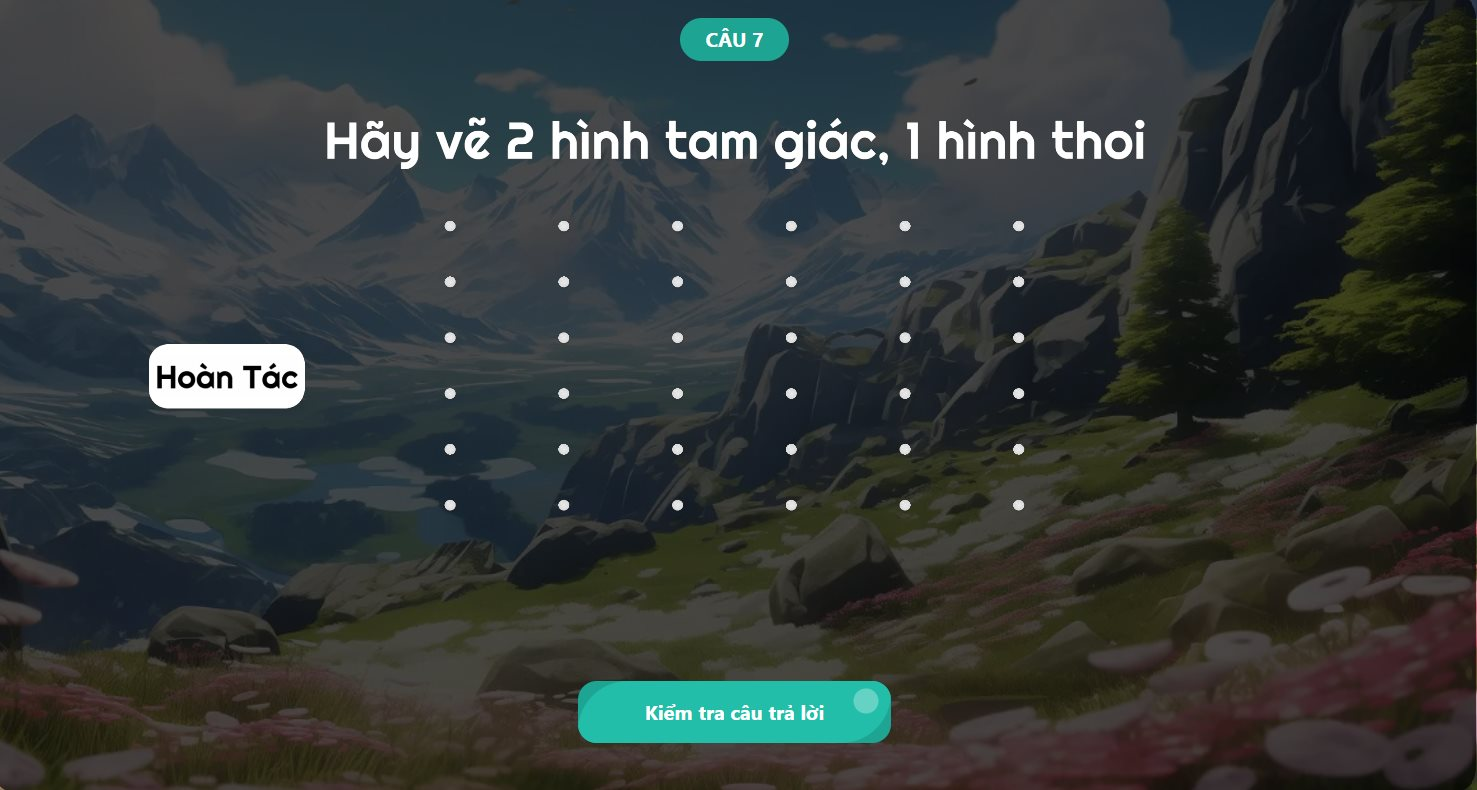
\includegraphics[width=0.9\textwidth]{Image/UI/Exercises/Geo.jpg}
	\caption{Dạng bài vẽ hình}
	\label{fig:geo}
\end{figure}

\subsubsection{Cơ sở học thuật xây dựng bài tập}

Nội dung các bài tập trong hệ thống được xây dựng dựa trên chương trình giáo dục môn Toán cấp Tiểu học của Bộ Giáo dục và Đào tạo. Mỗi chủ đề được phân chia theo ba mức độ nhận thức: \textbf{Nhận biết} (ghi nhớ, tái hiện thông tin), \textbf{Thông hiểu} (giải thích, áp dụng trực tiếp) và \textbf{Vận dụng} (phân tích, giải quyết vấn đề trong tình huống thực tế), nhằm đảm bảo tính phân hóa và phù hợp với từng trình độ học sinh.

% ===================== LỚP 1 =====================
\newpage
\paragraph{Lớp 1}
\renewcommand{\arraystretch}{1.3}
\begin{longtable}{|>{\centering\arraybackslash}m{0.8cm}|m{3.5cm}|>{\centering\arraybackslash}m{2cm}|m{7.5cm}|}
	\hline
	\textbf{STT} & \textbf{Chủ đề} & \textbf{Mức độ} & \textbf{Ví dụ minh họa} \\
	\hline
	\endfirsthead
	\hline
	\textbf{STT} & \textbf{Chủ đề} & \textbf{Mức độ} & \textbf{Ví dụ minh họa} \\
	\hline
	\endhead
	\hline
	\endfoot

	1 & Các số đến 10 và các phép tính cơ bản
	& Nhận biết & Viết các số từ 1 đến 10. (Ví dụ: Viết số 7) \\
	\cline{3-4}
	& & Thông hiểu & Thực hiện phép cộng/trừ đơn giản. ($5+3=?$ hoặc $8-2=?$) \\
	\cline{3-4}
	& & Vận dụng & Giải bài toán có lời văn. (Bạn An có 6 cái kẹo, mẹ cho thêm 4 cái. Hỏi An có tất cả bao nhiêu cái kẹo?) \\
	\hline

	2 & So sánh và các dấu toán học
	& Nhận biết & So sánh số lượng đồ vật. (Nhóm nào nhiều hơn, nhóm nào ít hơn?) \\
	\cline{3-4}
	& & Thông hiểu & Điền dấu thích hợp. ($5 \ldots 9$, điền dấu $<$, $>$, $=$ vào chỗ trống) \\
	\cline{3-4}
	& & Vận dụng & So sánh thực tế. (Bạn Lan có 7 viên bi, bạn Nam có 10 viên bi. Ai có nhiều hơn và nhiều hơn mấy viên?) \\
	\hline

	3 & Hình học cơ bản
	& Nhận biết & Chỉ ra các hình đã học. (Trong các hình sau, đâu là hình tam giác?) \\
	\cline{3-4}
	& & Thông hiểu & Đếm số lượng hình. (Trong hình vẽ này có bao nhiêu hình vuông?) \\
	\cline{3-4}
	& & Vận dụng & Ghép hình để tạo hình mới. (Ghép 2 hình tam giác lại, em được hình gì?) \\
	\hline

	4 & Vị trí và phương hướng
	& Nhận biết & Xác định vị trí. (Con mèo đang ở trên hay dưới cái ghế?) \\
	\cline{3-4}
	& & Thông hiểu & Mô tả vị trí của vật. (Con chim đang bay bên trái cái cây.) \\
	\cline{3-4}
	& & Vận dụng & Vẽ một quả bóng bên phải cái hộp và một bông hoa bên trên quả bóng. \\
	\hline

	5 & Các số có hai chữ số
	& Nhận biết & Viết số có hai chữ số. (Viết số "hai mươi lăm".) \\
	\cline{3-4}
	& & Thông hiểu & Phân tích cấu tạo số. (Trong số 37, số 3 thuộc hàng gì, số 7 thuộc hàng gì?) \\
	\cline{3-4}
	& & Vận dụng & Sắp xếp các số 25, 18, 32, 9 theo thứ tự từ bé đến lớn. \\
	\hline

	6 & Phép cộng, trừ trong phạm vi 100 (không nhớ)
	& Nhận biết & Thực hiện phép tính. ($23+6=?$ hoặc $45-20=?$) \\
	\cline{3-4}
	& & Thông hiểu & Điền số còn thiếu. ($40 + \ldots = 47$) \\
	\cline{3-4}
	& & Vận dụng & Bạn có 28 cái nhãn vở, mua thêm 11 cái. Hỏi bạn có tất cả bao nhiêu cái nhãn vở? \\
	\hline

	7 & Phép cộng, trừ có nhớ trong phạm vi 100
	& Nhận biết & Thực hiện phép tính. ($8+7=?$ hoặc $15-9=?$) \\
	\cline{3-4}
	& & Thông hiểu & Đặt tính rồi tính $19+24$ và $52-18$. \\
	\cline{3-4}
	& & Vận dụng & Lớp 1A có 24 học sinh, lớp 1B có 29 học sinh. Cả hai lớp có bao nhiêu học sinh? \\
	\hline

	8 & Đo lường cơ bản
	& Nhận biết & Dùng thước kẻ đo độ dài của một cây bút chì. \\
	\cline{3-4}
	& & Thông hiểu & An đo bàn được 5 gang, Bình đo được 6 gang. Bàn tay của ai lớn hơn? \\
	\cline{3-4}
	& & Vận dụng & Một sợi dây dài 20 cm, cắt đi 8 cm. Sợi dây còn lại dài bao nhiêu cm? \\
	\hline

	9 & Thời gian và xem đồng hồ
	& Nhận biết & Xem giờ đúng. (Đồng hồ chỉ mấy giờ?) \\
	\cline{3-4}
	& & Thông hiểu & An ăn sáng lúc 7 giờ, đi học lúc 8 giờ. Hoạt động nào diễn ra trước? \\
	\cline{3-4}
	& & Vận dụng & Bây giờ là 10 giờ. Sau 3 tiếng nữa sẽ là mấy giờ? \\
	\hline

	10 & Giải bài toán có lời văn
	& Nhận biết & Tóm tắt bài toán. (Có 5 con chim, 2 con bay đi. Còn lại bao nhiêu con? $5-2=?$) \\
	\cline{3-4}
	& & Thông hiểu & Có 5 quả táo trong giỏ, mẹ bỏ thêm 3 quả. Giỏ có bao nhiêu quả? \\
	\cline{3-4}
	& & Vận dụng & Nhà Mai có 10 con gà, bán 4 con, rồi mua thêm 2 con. Còn lại bao nhiêu con gà? \\
	\hline

	\caption{Các chủ đề toán lớp 1 theo chương trình Bộ GD\&ĐT}
	\label{tab:toan-lop1}
\end{longtable}

% ===================== LỚP 2 =====================
\paragraph{Lớp 2}
\renewcommand{\arraystretch}{1.3}
\begin{longtable}{|>{\centering\arraybackslash}m{0.8cm}|m{3.5cm}|>{\centering\arraybackslash}m{2cm}|m{7.5cm}|}
	\hline
	\textbf{STT} & \textbf{Chủ đề} & \textbf{Mức độ} & \textbf{Ví dụ minh họa} \\
	\hline
	\endfirsthead
	\hline
	\textbf{STT} & \textbf{Chủ đề} & \textbf{Mức độ} & \textbf{Ví dụ minh họa} \\
	\hline
	\endhead
	\hline
	\endfoot

	1 & Ôn tập phép cộng, trừ (có nhớ) trong phạm vi 100
	& Nhận biết & Thực hiện phép tính: $12+8=?$ \\
	\cline{3-4}
	& & Thông hiểu & Đặt tính rồi tính: $34+48$. \\
	\cline{3-4}
	& & Vận dụng & Một cửa hàng bán được 45 chiếc bánh mì buổi sáng, buổi chiều bán thêm 37 chiếc. Hỏi cả ngày bán được bao nhiêu chiếc? \\
	\hline

	2 & Cấu tạo phép tính
	& Nhận biết & Trong phép tính $25+13=38$, hãy chỉ ra số hạng và tổng. \\
	\cline{3-4}
	& & Thông hiểu & Phép tính $50-20=30$: đâu là số bị trừ, số trừ và hiệu? \\
	\cline{3-4}
	& & Vận dụng & Tìm số hạng còn thiếu: $15 + \ldots = 40$. \\
	\hline

	3 & Các số trong phạm vi 1\,000
	& Nhận biết & Đọc số 453. \\
	\cline{3-4}
	& & Thông hiểu & Viết số có hàng trăm là 2, hàng chục là 5, hàng đơn vị là 9. \\
	\cline{3-4}
	& & Vận dụng & Sắp xếp các số 325, 253, 532 theo thứ tự từ bé đến lớn. \\
	\hline

	4 & Phép cộng, trừ trong phạm vi 1\,000
	& Nhận biết & Thực hiện phép tính: $200+50=?$ \\
	\cline{3-4}
	& & Thông hiểu & Đặt tính rồi tính: $435+287$. \\
	\cline{3-4}
	& & Vận dụng & Thư viện có 560 quyển sách, nhà trường mua thêm 250 quyển. Hỏi thư viện có tất cả bao nhiêu quyển? \\
	\hline

	5 & Phép nhân và bảng nhân
	& Nhận biết & Chuyển phép cộng $2+2+2+2$ thành phép nhân. \\
	\cline{3-4}
	& & Thông hiểu & Tính tích của $5 \times 6$. \\
	\cline{3-4}
	& & Vận dụng & Mỗi bạn được phát 5 quyển vở. Hỏi 4 bạn sẽ nhận được bao nhiêu quyển vở? \\
	\hline

	6 & Phép chia và bảng chia
	& Nhận biết & Thực hiện phép chia: $10:2=?$ \\
	\cline{3-4}
	& & Thông hiểu & Phép tính nào đúng? (A) $10:5=2$ hoặc (B) $10:2=5$. \\
	\cline{3-4}
	& & Vận dụng & Có 25 cái kẹo, chia đều cho 5 bạn. Hỏi mỗi bạn được bao nhiêu cái kẹo? \\
	\hline

	7 & Đo lường (Độ dài và Khối lượng)
	& Nhận biết & Đọc và viết các đơn vị đo: 1 kg, 1 m, 1 dm. \\
	\cline{3-4}
	& & Thông hiểu & Đổi đơn vị đo: $1\,\text{m} = \ldots\,\text{dm}$. \\
	\cline{3-4}
	& & Vận dụng & Một khúc gỗ dài 20 m, người ta cưa đi 8 m. Hỏi khúc gỗ còn lại dài bao nhiêu mét? \\
	\hline

	8 & Hình học và đo lường
	& Nhận biết & Chỉ ra đâu là đường thẳng, đường cong, đường gấp khúc. \\
	\cline{3-4}
	& & Thông hiểu & Đo độ dài một đoạn thẳng bằng thước kẻ. \\
	\cline{3-4}
	& & Vận dụng & Tính độ dài đường gấp khúc gồm 3 đoạn thẳng dài lần lượt 20 cm, 15 cm, 10 cm. \\
	\hline

	9 & Thời gian và tiền tệ
	& Nhận biết & Xem đồng hồ chỉ 9 giờ 15 phút. \\
	\cline{3-4}
	& & Thông hiểu & Hôm nay là thứ ba. Hỏi ngày mai là thứ mấy? \\
	\cline{3-4}
	& & Vận dụng & Bây giờ là 8 giờ. Sau 15 phút nữa sẽ là mấy giờ? \\
	\hline

	10 & Thống kê và xác suất
	& Nhận biết & Biểu đồ tranh dưới đây cho biết có bao nhiêu quả táo? \\
	\cline{3-4}
	& & Thông hiểu & Lập bảng kiểm đếm số lượng bạn trai, bạn gái trong lớp. \\
	\cline{3-4}
	& & Vận dụng & Gieo một con xúc xắc: chắc chắn, có thể hay không thể ra mặt có 7 chấm? \\
	\hline

	\caption{Các chủ đề toán lớp 2 theo chương trình Bộ GD\&ĐT}
	\label{tab:toan-lop2}
\end{longtable}

% ===================== LỚP 3 =====================
\paragraph{Lớp 3}
\renewcommand{\arraystretch}{1.3}
\begin{longtable}{|>{\centering\arraybackslash}m{0.8cm}|m{3.5cm}|>{\centering\arraybackslash}m{2cm}|m{7.5cm}|}
	\hline
	\textbf{STT} & \textbf{Chủ đề} & \textbf{Mức độ} & \textbf{Ví dụ minh họa} \\
	\hline
	\endfirsthead
	\hline
	\textbf{STT} & \textbf{Chủ đề} & \textbf{Mức độ} & \textbf{Ví dụ minh họa} \\
	\hline
	\endhead
	\hline
	\endfoot

	1 & Hoàn thiện bảng nhân, bảng chia
	& Nhận biết & $7 \times 8 = ?$ \\
	\cline{3-4}
	& & Thông hiểu & Tìm số bị chia trong phép chia: $\ldots : 4 = 9$. \\
	\cline{3-4}
	& & Vận dụng & Có 35 bông hoa, cắm vào các lọ, mỗi lọ 5 bông. Hỏi cắm được bao nhiêu lọ hoa? \\
	\hline

	2 & Phân số cơ bản
	& Nhận biết & Tô màu vào $\dfrac{1}{3}$ hình tròn sau. \\
	\cline{3-4}
	& & Thông hiểu & Sắp xếp các phân số theo thứ tự từ bé đến lớn: $\dfrac{1}{2}$, $\dfrac{1}{4}$, $\dfrac{1}{3}$. \\
	\cline{3-4}
	& & Vận dụng & Mẹ có 12 quả cam, cho An $\dfrac{1}{4}$ số cam đó. Hỏi mẹ đã cho An bao nhiêu quả cam? \\
	\hline

	3 & Các số trong phạm vi 100\,000
	& Nhận biết & Viết số "mười hai nghìn không trăm năm mươi tư". \\
	\cline{3-4}
	& & Thông hiểu & Phân tích cấu tạo số: 45\,782 gồm bao nhiêu nghìn, trăm, chục, đơn vị? \\
	\cline{3-4}
	& & Vận dụng & Sắp xếp các số 23\,456; 23\,546; 23\,465 theo thứ tự từ lớn đến bé. \\
	\hline

	4 & Cộng, trừ, nhân, chia trong phạm vi 100\,000
	& Nhận biết & $25\,431 + 10\,520 = ?$ \\
	\cline{3-4}
	& & Thông hiểu & Đặt tính rồi tính $15\,328 \times 4$ và $48\,576 : 6$. \\
	\cline{3-4}
	& & Vận dụng & Một xưởng may sản xuất 12\,560 chiếc áo tháng đầu, tháng thứ hai sản xuất nhiều hơn 2\,500 chiếc. Hỏi cả hai tháng sản xuất được bao nhiêu chiếc? \\
	\hline

	5 & Tìm thành phần chưa biết của phép tính
	& Nhận biết & Tìm $x$ trong phép tính $x + 15 = 20$. \\
	\cline{3-4}
	& & Thông hiểu & Tìm $x$ trong phép tính $x : 7 = 8$. \\
	\cline{3-4}
	& & Vận dụng & Tìm $x$ trong phép tính $100 - x = 25 \times 3$. \\
	\hline

	6 & Giải toán với biểu thức và hai bước tính
	& Nhận biết & Tính giá trị của biểu thức: $500 + 50 \times 2$. \\
	\cline{3-4}
	& & Thông hiểu & An có 20 viên bi, Bình có gấp 3 lần số bi của An. Hỏi Bình có bao nhiêu viên bi? \\
	\cline{3-4}
	& & Vận dụng & Một cửa hàng có 500 kg gạo tẻ, đã bán 250 kg và còn lại $\dfrac{1}{2}$ số gạo đã bán. Hỏi ban đầu cửa hàng có bao nhiêu kg gạo? \\
	\hline

	7 & Hình học cơ bản
	& Nhận biết & Đâu là góc vuông, đâu là góc không vuông? \\
	\cline{3-4}
	& & Thông hiểu & Vẽ một đoạn thẳng AB dài 5 cm. \\
	\cline{3-4}
	& & Vận dụng & Vẽ một hình chữ nhật có chiều dài 8 cm và chiều rộng 5 cm. \\
	\hline

	8 & Chu vi và diện tích
	& Nhận biết & Tính chu vi của hình vuông có cạnh dài 5 cm. \\
	\cline{3-4}
	& & Thông hiểu & Tính diện tích của hình chữ nhật có chiều dài 10 cm và chiều rộng 6 cm. \\
	\cline{3-4}
	& & Vận dụng & Một mảnh vườn hình chữ nhật dài 20 m, rộng 15 m. Người ta rào lưới xung quanh. Hỏi cần bao nhiêu mét lưới? \\
	\hline

	9 & Đo lường (Độ dài, khối lượng, dung tích, nhiệt độ)
	& Nhận biết & Viết ký hiệu của đơn vị đo: mililitre. \\
	\cline{3-4}
	& & Thông hiểu & Đổi đơn vị: $3\,\text{kg} = \ldots\,\text{g}$. \\
	\cline{3-4}
	& & Vận dụng & Một xe tải chở 1\,500 kg gạo và thêm 500 kg ngô. Hỏi xe tải chở tất cả bao nhiêu tạ? (biết $1\,\text{tạ} = 100\,\text{kg}$) \\
	\hline

	10 & Thống kê và xác suất
	& Nhận biết & Theo biểu đồ, lớp 2 có bao nhiêu học sinh? \\
	\cline{3-4}
	& & Thông hiểu & Lập bảng thống kê số lượng các loại quả: 3 quả táo, 2 quả cam, 4 quả dứa. \\
	\cline{3-4}
	& & Vận dụng & Khi gieo một đồng xu, khả năng nào sẽ xảy ra: chắc chắn ra mặt sấp, có thể ra mặt sấp, hay không thể ra mặt sấp? \\
	\hline

	\caption{Các chủ đề toán lớp 3 theo chương trình Bộ GD\&ĐT}
	\label{tab:toan-lop3}
\end{longtable}

% ===================== LỚP 4 =====================
\paragraph{Lớp 4}
\renewcommand{\arraystretch}{1.3}
\begin{longtable}{|>{\centering\arraybackslash}m{0.8cm}|m{3.5cm}|>{\centering\arraybackslash}m{2cm}|m{7.5cm}|}
	\hline
	\textbf{STT} & \textbf{Chủ đề} & \textbf{Mức độ} & \textbf{Ví dụ minh họa} \\
	\hline
	\endfirsthead
	\hline
	\textbf{STT} & \textbf{Chủ đề} & \textbf{Mức độ} & \textbf{Ví dụ minh họa} \\
	\hline
	\endhead
	\hline
	\endfoot

	1 & Các số tự nhiên có nhiều chữ số
	& Nhận biết & Đọc và viết số có nhiều chữ số. (Ví dụ: "một trăm hai mươi ba triệu...") \\
	\cline{3-4}
	& & Thông hiểu & Xác định giá trị vị trí. (Ví dụ: Chữ số 5 trong 123\,456\,789 có giá trị là 500\,000.) \\
	\cline{3-4}
	& & Vận dụng & So sánh và sắp xếp các số có nhiều chữ số theo thứ tự. \\
	\hline

	2 & Các phép tính với số tự nhiên
	& Nhận biết & Thực hiện bốn phép tính cơ bản với các số lớn, kể cả phép chia có dư. \\
	\cline{3-4}
	& & Thông hiểu & Vận dụng tính chất giao hoán, kết hợp để tính nhẩm nhanh. (Ví dụ: $25 \times 36 \times 4$) \\
	\cline{3-4}
	& & Vận dụng & Tìm số bị chia, số chia trong phép chia có dư. \\
	\hline

	3 & Số trung bình cộng
	& Nhận biết & Nắm vững công thức tính trung bình cộng. \\
	\cline{3-4}
	& & Thông hiểu & Tính trung bình cộng của dãy số: 10, 20, 30, 40. \\
	\cline{3-4}
	& & Vận dụng & Một đội ngày đầu trồng 200 cây, ngày thứ hai trồng 300 cây. Trung bình mỗi ngày trồng được bao nhiêu cây? \\
	\hline

	4 & Phân số và các phép tính cơ bản
	& Nhận biết & Nhận biết khái niệm phân số: tử số, mẫu số. \\
	\cline{3-4}
	& & Thông hiểu & Rút gọn phân số và quy đồng mẫu số. \\
	\cline{3-4}
	& & Vận dụng & So sánh các phân số khác mẫu số. \\
	\hline

	5 & Các phép tính với phân số
	& Nhận biết & Cộng, trừ, nhân, chia phân số cùng mẫu số. \\
	\cline{3-4}
	& & Thông hiểu & Cộng, trừ phân số khác mẫu số sau khi quy đồng. \\
	\cline{3-4}
	& & Vận dụng & Một tấm vải dài $\frac{3}{4}$ m, cắt đi $\frac{1}{2}$ m. Hỏi tấm vải còn lại dài bao nhiêu mét? \\
	\hline

	6 & Hình học cơ bản
	& Nhận biết & Nhận biết và gọi tên hình bình hành, hình thoi. \\
	\cline{3-4}
	& & Thông hiểu & Phân biệt góc nhọn, góc tù, góc bẹt; đường thẳng vuông góc, song song. \\
	\cline{3-4}
	& & Vận dụng & Vẽ hình theo yêu cầu. \\
	\hline

	7 & Chu vi và diện tích
	& Nhận biết & Công thức tính chu vi và diện tích hình vuông, hình chữ nhật. \\
	\cline{3-4}
	& & Thông hiểu & Chuyển đổi đơn vị đo diện tích (m$^2$, dm$^2$). \\
	\cline{3-4}
	& & Vận dụng & Tính chu vi và diện tích trong tình huống thực tế, kể cả bài toán ghép hình. \\
	\hline

	8 & Đo lường (Khối lượng và thời gian)
	& Nhận biết & Các đơn vị đo khối lượng lớn: yến, tạ, tấn; thời gian: thế kỷ, giây. \\
	\cline{3-4}
	& & Thông hiểu & Chuyển đổi đơn vị. (Ví dụ: $1\,\text{tấn} = \ldots\,\text{kg}$) \\
	\cline{3-4}
	& & Vận dụng & Một xe tải chở 5 tấn hàng, đã dỡ 2 tạ. Trên xe còn lại bao nhiêu kg hàng? \\
	\hline

	9 & Thống kê và biểu đồ
	& Nhận biết & Đọc và hiểu thông tin từ biểu đồ cột. \\
	\cline{3-4}
	& & Thông hiểu & Lập bảng thống kê từ một dãy số liệu. \\
	\cline{3-4}
	& & Vận dụng & Phân tích biểu đồ: lớp nào có nhiều học sinh giỏi nhất? \\
	\hline

	10 & Toán nâng cao và biểu thức
	& Nhận biết & Bài toán tìm hai số khi biết tổng và hiệu. \\
	\cline{3-4}
	& & Thông hiểu & Tính giá trị biểu thức: $a + b \times 5$ khi $a=10$, $b=2$. \\
	\cline{3-4}
	& & Vận dụng & Bài toán rút về đơn vị. (Ví dụ: 3 kg táo hết 60\,000 đồng. Hỏi 5 kg hết bao nhiêu tiền?) \\
	\hline

	\caption{Các chủ đề toán lớp 4 theo chương trình Bộ GD\&ĐT}
	\label{tab:toan-lop4}
\end{longtable}

% ===================== LỚP 5 =====================
\paragraph{Lớp 5}
\renewcommand{\arraystretch}{1.3}
\begin{longtable}{|>{\centering\arraybackslash}m{0.8cm}|m{3.5cm}|>{\centering\arraybackslash}m{2cm}|m{7.5cm}|}
	\hline
	\textbf{STT} & \textbf{Chủ đề} & \textbf{Mức độ} & \textbf{Ví dụ minh họa} \\
	\hline
	\endfirsthead
	\hline
	\textbf{STT} & \textbf{Chủ đề} & \textbf{Mức độ} & \textbf{Ví dụ minh họa} \\
	\hline
	\endhead
	\hline
	\endfoot

	1 & Ôn tập và bổ sung kiến thức
	& Nhận biết & Một đội công nhân sửa đường, ngày đầu sửa được 120 m, ngày thứ hai sửa nhiều hơn ngày đầu 15 m. Hỏi ngày thứ hai sửa được bao nhiêu mét đường? \\
	\cline{3-4}
	& & Thông hiểu & Một tấm vải dài 30 m, đã bán được $\dfrac{2}{3}$ tấm vải. Hỏi còn lại bao nhiêu mét vải? \\
	\cline{3-4}
	& & Vận dụng & Một cửa hàng bán gạo buổi sáng 500 kg, buổi chiều bán $\dfrac{1}{2}$ số gạo buổi sáng. Hỏi cả hai buổi cửa hàng bán được bao nhiêu tạ gạo? \\
	\hline

	2 & Số thập phân
	& Nhận biết & Viết các số: "Năm phẩy bảy mươi lăm" và "Bốn trăm năm mươi sáu phẩy không không tám". \\
	\cline{3-4}
	& & Thông hiểu & Sắp xếp theo thứ tự từ lớn đến bé: 12,3; 12,03; 12,31; 12,13. \\
	\cline{3-4}
	& & Vận dụng & Dùng 3 chữ số 0, 5, 8 và dấu phẩy, hãy viết tất cả các số thập phân có hai chữ số ở phần thập phân và lớn hơn 50. \\
	\hline

	3 & Các phép tính với số thập phân
	& Nhận biết & Thực hiện phép tính: $15{,}4 + 8{,}9 = ?$ \\
	\cline{3-4}
	& & Thông hiểu & Mẹ mua cá hết 56\,500 đồng và mua rau hết 15\,500 đồng, đưa 100\,000 đồng. Hỏi mẹ được trả lại bao nhiêu tiền? \\
	\cline{3-4}
	& & Vận dụng & Một mảnh đất hình chữ nhật dài 25,5 m, chiều rộng bằng $\dfrac{2}{3}$ chiều dài. Tính chu vi và diện tích mảnh đất đó. \\
	\hline

	4 & Tỉ số và tỉ lệ
	& Nhận biết & Một lớp học có 20 bạn nam và 25 bạn nữ. Tìm tỉ số của số bạn nam và số bạn nữ. \\
	\cline{3-4}
	& & Thông hiểu & Lãi suất tiết kiệm là 0,5\% một tháng. Cô Lan gửi 10 triệu đồng. Hỏi sau một tháng cô nhận được bao nhiêu tiền lãi? \\
	\cline{3-4}
	& & Vận dụng & Tổng số tuổi của hai anh em là 36 tuổi. Tuổi em bằng $\dfrac{4}{5}$ tuổi anh. Tính tuổi của mỗi người. \\
	\hline

	5 & Hình học phẳng nâng cao
	& Nhận biết & Một hình tam giác có đáy 10 cm, chiều cao 8 cm. Tính diện tích hình tam giác đó. \\
	\cline{3-4}
	& & Thông hiểu & Một hình tròn có bán kính 5 dm. Tính chu vi và diện tích hình tròn đó. \\
	\cline{3-4}
	& & Vận dụng & Một mảnh đất hình thang có tổng độ dài hai đáy là 40 m, chiều cao 25 m. Tính diện tích mảnh đất. \\
	\hline

	6 & Hình học không gian cơ bản
	& Nhận biết & Một hình lập phương có cạnh 4 cm. Tính thể tích hình lập phương đó. \\
	\cline{3-4}
	& & Thông hiểu & Một hình hộp chữ nhật dài 12 m, rộng 8 m, cao 5 m. Tính diện tích xung quanh và diện tích toàn phần. \\
	\cline{3-4}
	& & Vận dụng & Một bể cá hình hộp chữ nhật dài 1,2 m, rộng 0,8 m, cao 1 m. Người ta đổ nước sao cho mực nước bằng $\dfrac{3}{4}$ chiều cao bể. Tính thể tích nước trong bể. \\
	\hline

	7 & Đo lường
	& Nhận biết & Đổi đơn vị: $12\,\text{tấn} = \ldots\,\text{kg}$. \\
	\cline{3-4}
	& & Thông hiểu & Một xe chở 5 tấn 50 kg gạo, lần đầu dỡ 2\,500 kg. Hỏi trên xe còn lại bao nhiêu tạ gạo? \\
	\cline{3-4}
	& & Vận dụng & Một ô tô đi từ A lúc 7 giờ 30 phút, đến B lúc 10 giờ 15 phút, dọc đường nghỉ 30 phút. Hỏi thời gian ô tô đi thực tế là bao lâu? \\
	\hline

	8 & Toán chuyển động đều
	& Nhận biết & Một người đi bộ vận tốc 5 km/giờ. Hỏi sau 2 giờ đi được bao nhiêu km? \\
	\cline{3-4}
	& & Thông hiểu & Một xe máy đi từ A đến B với vận tốc 40 km/giờ hết 2 giờ, sau đó quay về A với vận tốc 50 km/giờ. Tính thời gian xe đi từ B về A. \\
	\cline{3-4}
	& & Vận dụng & Hai ô tô khởi hành cùng lúc từ A và B (cách nhau 210 km) đi ngược chiều nhau. Vận tốc xe từ A là 50 km/giờ, xe từ B là 60 km/giờ. Hỏi sau bao lâu hai xe gặp nhau? \\
	\hline

	9 & Thống kê và xác suất
	& Nhận biết & Biểu đồ cho biết số học sinh thích môn bóng đá là bao nhiêu? \\
	\cline{3-4}
	& & Thông hiểu & Khối lớp 5 có 150 học sinh, trong đó 60 bạn nữ. Biểu diễn tỉ số phần trăm số bạn nữ và bạn nam bằng biểu đồ quạt. \\
	\cline{3-4}
	& & Vận dụng & Trong một hộp có 5 viên bi đỏ và 3 viên bi xanh. Không nhìn vào hộp, lấy ngẫu nhiên 1 viên. Việc lấy được bi đỏ có chắc chắn, có thể hay không thể xảy ra? \\
	\hline

	10 & Ứng dụng toán học vào thực tiễn
	& Nhận biết & Trên bản đồ tỉ lệ 1:1\,000, khoảng cách A và B là 5 cm. Hỏi khoảng cách thực tế là bao nhiêu mét? \\
	\cline{3-4}
	& & Thông hiểu & Một người gửi tiết kiệm 50 triệu đồng với lãi suất 0,6\% một tháng. Hỏi sau 2 tháng rút cả vốn lẫn lãi được bao nhiêu tiền? \\
	\cline{3-4}
	& & Vận dụng & Bác An mua tivi giá 10 triệu đồng, trả trước 40\%. Số còn lại trả góp trong 5 tháng đều nhau. Hỏi mỗi tháng bác phải trả bao nhiêu tiền? \\
	\hline

	\caption{Các chủ đề toán lớp 5 theo chương trình Bộ GD\&ĐT}
	\label{tab:toan-lop5}
\end{longtable}

\subsubsection{Ánh xạ dạng bài tập với chủ đề học thuật}

Bảng dưới đây thể hiện sự tương ứng giữa 18 dạng bài tập tương tác đã hiện thực và các chủ đề trong chương trình toán tiểu học. Ký hiệu \textbf{C\textit{n}} chỉ chủ đề thứ $n$ theo thứ tự trong bảng của từng lớp.

\renewcommand{\arraystretch}{1.35}
\begin{longtable}{|m{3.5cm}|>{\centering\arraybackslash}m{1.5cm}|>{\centering\arraybackslash}m{1.5cm}|>{\centering\arraybackslash}m{1.5cm}|>{\centering\arraybackslash}m{1.5cm}|>{\centering\arraybackslash}m{1.5cm}|m{3.5cm}|}
	\hline
	\textbf{Dạng bài tập} & \textbf{Lớp 1} & \textbf{Lớp 2} & \textbf{Lớp 3} & \textbf{Lớp 4} & \textbf{Lớp 5} & \textbf{Ghi chú} \\
	\hline
	\endfirsthead
	\hline
	\textbf{Dạng bài tập} & \textbf{Lớp 1} & \textbf{Lớp 2} & \textbf{Lớp 3} & \textbf{Lớp 4} & \textbf{Lớp 5} & \textbf{Ghi chú} \\
	\hline
	\endhead
	\hline
	\endfoot

	Trắc nghiệm \newline (Multiple Choice)
	& C1--C10 & C1--C10 & C1--C10 & C1--C10 & C1--C10
	& Áp dụng cho toàn bộ chủ đề \\
	\hline

	Ghép cặp \newline (Matching)
	& C2, C3 & C5, C6 & C1, C2 & C4, C6 & C4, C5
	& Ghép số, ghép hình, ghép phép tính tương đương \\
	\hline

	Điền số \newline (Fill in the Blanks)
	& C1, C6, C7 & C1, C2, C4 & C4, C5 & C2, C3 & C1, C3
	& Điền kết quả phép tính, tìm thành phần còn thiếu \\
	\hline

	Kéo thả \newline (Drag and Drop)
	& C1, C5 & C3, C4 & C3, C4 & C1, C2 & C2, C3
	& Điền số vào biểu thức, sắp xếp dãy số \\
	\hline

	Phân loại \newline (Grouping)
	& C1, C5 & C3 & C3 & C1 & C2
	& Phân loại chẵn/lẻ, phân loại hình, phân loại theo nhóm \\
	\hline

	Đúng/Sai \newline (True/False)
	& C2, C6, C7 & C1, C4, C5, C6 & C1, C4, C5 & C2, C4, C5 & C1, C3, C4
	& Kiểm tra tính đúng đắn của một phép tính hoặc mệnh đề so sánh \\
	\hline

	Tổ hợp Burger \newline (Burger)
	& -- & C10 & C10 & C10 & C9
	& Thống kê, xác suất tổ hợp \\
	\hline

	Xe buýt \newline (Bus)
	& C6 & C1, C4 & C4 & C2 & --
	& Cộng số tròn chục/tròn trăm; xếp hàng lên xe \\
	\hline

	Bắt chim \newline (Catch Bird)
	& C1, C6, C7 & C1, C4, C5 & C1, C4 & C2, C3 & C1, C3
	& Dạng tổng quát; biểu diễn nhiều dạng toán bằng cơ chế bắt chim \\
	\hline

	Đồng hồ \newline (Clock)
	& C9 & C9 & -- & C8 & C7
	& Đọc giờ kim, giờ số; tính thời gian \\
	\hline

	Đổi tiền xu \newline (Coin)
	& -- & C9 & -- & C8 & C10
	& Nhận biết mệnh giá, đổi tiền, tính toán với tiền tệ \\
	\hline

	Viên bi \newline (Gumball)
	& C1, C2 & C10 & C10 & C9 & C9
	& Đếm, so sánh số lượng; thống kê trực quan \\
	\hline

	Cân thủ công \newline (Manual Scale)
	& C2 & C7 & C9 & C8 & C7
	& So sánh lớn hơn/bé hơn/bằng nhau qua cân \\
	\hline

	Chia pizza \newline (Pizza)
	& -- & -- & C2 & C4, C5 & C4
	& Làm quen phân số, tỉ lệ qua hình ảnh trực quan \\
	\hline

	Thả chim \newline (Release Bird)
	& C1--C10 & C1--C10 & C1--C10 & C1--C10 & C1--C10
	& Áp dụng cho toàn bộ chủ đề \\
	\hline

	Cân điện tử \newline (Scale)
	& C6, C7 & C1, C4 & C4 & C2 & C3
	& Cộng/trừ qua cân bằng; có thể có nhiều đáp án đúng \\
	\hline

	Tưới cây \newline (Tree)
	& C10 & C2 & C6 & C10 & C10
	& Bài toán nhiều bước; tưới từng bước để hoàn thành \\
	\hline

	Vẽ hình \newline (Geo)
	& C3 & C8 & C7, C8 & C6, C7 & C5
	& Vẽ hình học; tính chu vi, diện tích \\
	\hline

	\caption{Ánh xạ giữa 18 dạng bài tập và chủ đề chương trình Bộ GD\&ĐT}
	\label{tab:exercise-mapping}
\end{longtable}

Kết quả phân tích bảng ánh xạ cho thấy hệ thống bài tập đạt được độ bao phủ toàn diện trên toàn bộ chương trình toán tiểu học. Với \textbf{18 dạng tương tác} được phân phối trải rộng qua \textbf{5 khối lớp} và \textbf{10 chủ đề học thuật} mỗi lớp, mọi đơn vị kiến thức trong chương trình của Bộ Giáo dục và Đào tạo đều có ít nhất một dạng bài tập phù hợp để luyện tập.
Điểm nhấn quan trọng trong thiết kế là hệ thống đề cao \textbf{tư duy linh hoạt}: nhiều dạng bài chấp nhận \textbf{nhiều cách giải khác nhau} miễn là kết quả cuối cùng là đúng, phản ánh đúng bản chất của toán học là khuyến khích học sinh tự tìm con đường tư duy của mình thay vì rập khuôn một đáp án duy nhất.
Ba mức độ nhận thức \textbf{Nhận biết -- Thông hiểu -- Vận dụng} được duy trì xuyên suốt theo đúng chuẩn chương trình của Bộ Giáo dục và Đào tạo, giúp hệ thống phục vụ toàn dải trình độ: từ học sinh mới làm quen khái niệm đến học sinh cần thử thách ở mức phân tích và giải quyết vấn đề thực tế. Sự kết hợp giữa độ bao phủ rộng theo chương trình, tính chuyên biệt theo từng miền kiến thức và triết lý tôn trọng tư duy đa hướng là nền tảng để hệ thống không chỉ dạy toán mà còn \textbf{rèn luyện cách suy nghĩ} cho học sinh tiểu học.


 
 % Chuong 6
 \newpage
\section{Hiện thực}
Chương này tập trung trình bày các giải pháp công nghệ và hạ tầng kỹ thuật được áp dụng để hiện thực hóa và triển khai hệ thống. Việc lựa chọn các công nghệ này đóng vai trò quyết định đến tính ổn định trong vận hành, đồng thời đảm bảo khả năng đáp ứng trọn vẹn các yêu cầu đã được đề ra.

\subsection{Công nghệ sử dụng}
\subsubsection{Giao diện người dùng}

\begin{itemize}
  \item \textbf{Next.js (React)}
    \begin{itemize}
      \item \textbf{Giới thiệu:} Next.js là một framework React mã nguồn mở được phát triển bởi Vercel, hỗ trợ rendering phía server (SSR) và tạo trang tĩnh (SSG) \cite{nextjsdocs}.
      \item \textbf{Lý do sử dụng:} Next.js có khả năng tối ưu hiệu năng với Server-Side Rendering và Static Site Generation, giúp trang web load nhanh và thân thiện với SEO, ngoài ra framework này còn hỗ trợ routing tự động, API routes tích hợp sẵn, và có hệ sinh thái React phong phú với nhiều thư viện UI component \cite{nextjsdocs}. Next.js cho phép phát triển full-stack với cả frontend và backend API trong cùng một dự án, giúp đơn giản hóa quá trình phát triển. Ngoài ra, việc triển khai lên Vercel hoặc các nền tảng cloud khác rất dễ dàng, có cộng đồng hỗ trợ lớn và được cập nhật thường xuyên. Nhược điểm chính là learning curve cao hơn so với React thuần, nhưng đổi lại mang lại hiệu năng và trải nghiệm người dùng vượt trội.
    \end{itemize}
    
  \item \textbf{Cocos Creator}
    \begin{itemize}
      \item \textbf{Giới thiệu:} Cocos Creator là một game engine đa nền tảng mã nguồn mở, chuyên dụng cho phát triển game 2D/3D và các ứng dụng tương tác \cite{cocoscreator38}.
      \item \textbf{Lý do sử dụng:} Cocos Creator được sử dụng để tạo các bài tập tương tác (interactive exercises) và minigames với đồ họa phong phú, animation mượt mà. Engine này hỗ trợ export ra WebGL để chạy trực tiếp trên trình duyệt web, tích hợp dễ dàng với Next.js. Cocos Creator cung cấp editor trực quan giúp thiết kế game nhanh chóng, hỗ trợ physics engine tích hợp sẵn, và có khả năng xử lý nhiều đối tượng game cùng lúc với hiệu năng cao \cite{cocoscreator38}. Điều này rất phù hợp cho việc tạo các trò chơi toán học tương tác, bài tập kéo thả, và các minigame giáo dục hấp dẫn.
    \end{itemize}

  \item \textbf{Colyseus}
    \begin{itemize}
      \item \textbf{Giới thiệu:} Colyseus là một framework mã nguồn mở chuyên dụng cho việc xây dựng máy chủ game đa người chơi thời gian thực (real-time multiplayer), được phát triển trên nền tảng Node.js và sử dụng giao thức WebSocket để truyền tải dữ liệu hai chiều với độ trễ thấp.
      \item \textbf{Lý do sử dụng:} Trong hệ thống Dino Math, Colyseus được tích hợp để hỗ trợ tính năng minigame tương tác giữa hai người chơi, cụ thể là minigame \textbf{Tomato Shooting} -- trò chơi đối kháng thời gian thực lấy ý tưởng từ Gunny, trong đó hai người chơi cạnh tranh trả lời các phép tính toán học bằng cách bắn trúng đáp án đúng trước đối thủ. Colyseus cung cấp cơ chế quản lý \textit{Room} (phòng chơi) cho phép nhóm nhiều người chơi vào cùng một phiên game, đồng bộ hóa trạng thái game (game state) giữa tất cả các client thông qua \textit{Schema} -- một cấu trúc dữ liệu được tối ưu để chỉ truyền phần dữ liệu thay đổi (delta), giảm thiểu băng thông. Client Colyseus được tích hợp trực tiếp vào Cocos Creator thông qua SDK chính thức, giúp việc đồng bộ trạng thái game giữa server và engine trở nên liền mạch. Bên cạnh đó, Colyseus hỗ trợ cơ chế \textit{matchmaking} đơn giản, cho phép tự động ghép cặp hai người chơi vào cùng một phòng, cũng như xử lý các tình huống ngắt kết nối và tái kết nối (reconnect) một cách graceful.
    \end{itemize}
\end{itemize}


\subsubsection{Công nghệ Backend và Quản lý dữ liệu}
\begin{itemize}
	\item \textbf{Node.js \& Express.js}
	\begin{itemize}
		\item \textbf{Giới thiệu:} Node.js là một môi trường thực thi JavaScript phía server dựa trên V8 engine của Chrome, trong khi Express.js là một framework ứng dụng web tối giản, linh hoạt chạy trên nền tảng Node.js \cite{nodejs, expressjs}.
		\item \textbf{Lý do sử dụng:} Sự kết hợp giữa Node.js và Express.js cho phép xây dựng các dịch vụ API có hiệu suất cao nhờ cơ chế hướng sự kiện (event-driven) và I/O không chặn (non-blocking I/O). Điều này đặc biệt quan trọng đối với các tính năng thời gian thực trong Đấu trường, nơi cần xử lý đồng thời nhiều kết nối từ học sinh. Theo tài liệu chính thức \cite{expressjs}, Express.js cung cấp hệ thống Middleware mạnh mẽ, giúp nhóm dễ dàng quản lý luồng dữ liệu, xác thực người dùng và tích hợp các dịch vụ bên thứ ba một cách nhất quán. Việc sử dụng ngôn ngữ TypeScript đồng bộ từ Frontend đến Backend giúp giảm thiểu sai sót về kiểu dữ liệu và tăng tốc độ phát triển dự án.
	\end{itemize}
	
	\item \textbf{MongoDB} 
	\begin{itemize}
		\item \textbf{Giới thiệu:} MongoDB là hệ quản trị cơ sở dữ liệu NoSQL hướng tài liệu (document-oriented), lưu trữ dữ liệu dưới dạng các tài liệu có cấu trúc tương tự JSON \cite{mongodb}.
		\item \textbf{Lý do sử dụng:} MongoDB đóng vai trò là cơ sở dữ liệu chính để lưu trữ thông tin người dùng, kho câu hỏi, kết quả học tập và dữ liệu thống kê. Với tính chất \textit{schema-less}, MongoDB cho phép lưu trữ các định dạng câu hỏi toán học đa dạng (kéo thả, trắc nghiệm, điền số) mà không cần cấu trúc bảng cứng nhắc. Hệ thống tận dụng Mongoose ODM để giao tiếp giữa Node.js và cơ sở dữ liệu, giúp quản lý dữ liệu chặt chẽ hơn qua các định nghĩa Schema. Ngoài ra, khả năng mở rộng ngang (horizontal scaling) và Aggregation Pipeline mạnh mẽ của MongoDB hỗ trợ hiệu quả cho việc xử lý các truy vấn phức tạp như tính toán độ chính xác trung bình và thống kê lịch sử làm bài của học sinh.
	\end{itemize}
	
	\item \textbf{Redis} 
	\begin{itemize}
		\item \textbf{Giới thiệu:} Redis là hệ thống lưu trữ dữ liệu cấu trúc key-value dưới dạng in-memory (lưu trữ trên RAM), thường được dùng làm bộ nhớ đệm (caching) \cite{redis}.
		\item \textbf{Lý do sử dụng:} Redis được tích hợp để tối ưu hóa tốc độ phản hồi của hệ thống thông qua việc lưu trữ các dữ liệu có tần suất truy cập cao nhưng ít thay đổi hoặc các dữ liệu mang tính tạm thời như phiên đăng nhập (session). Đặc biệt, trong tính năng Đấu trường, Redis hỗ trợ tính toán và hiển thị bảng xếp hạng (leaderboard) theo thời gian thực với độ trễ cực thấp, mang lại trải nghiệm mượt mà cho học sinh khi tham gia thi đấu.
	\end{itemize}
\end{itemize}

\newpage
\subsubsection{Dịch vụ bên ngoài}
\begin{itemize}
  \item \textbf{Payment Gateway}
    \begin{itemize}
      \item \textbf{Giới thiệu:} Dịch vụ thanh toán trực tuyến của bên thứ ba (VNPay).
      \item \textbf{Lý do sử dụng:} Xử lý các giao dịch thanh toán cho việc đăng ký Premium một cách an toàn và tuân thủ các tiêu chuẩn bảo mật PCI DSS. Hỗ trợ nhiều phương thức thanh toán phổ biến tại Việt Nam như chuyển khoản ngân hàng, QR code, và ví điện tử. Cung cấp webhook để cập nhật trạng thái thanh toán real-time.
    \end{itemize}
    \item \textbf{Gmail}
    \begin{itemize}
    	\item \textbf{Giới thiệu:} Dịch vụ thư điện tử phổ biến hiện nay của Google.
    	\item \textbf{Lý do sử dụng:} Hỗ trợ việc xác thực danh tính người dùng bằng cách gửi mã xác thực qua email, được dùng cho tính năng đổi hoặc khôi phục mật khẩu.
    \end{itemize}
    \item \textbf{Google OAuth 2.0}
    \begin{itemize}
    	\item \textbf{Giới thiệu:} Cơ thức ủy quyền bảo mật cho phép người dùng chia sẻ tài liệu hoặc quyền truy cập từ tài khoản Google của mình cho các ứng dụng khác mà không cần tiết lộ mật khẩu cá nhân.
    	\item \textbf{Lý do sử dụng:} Được sử dụng cho tính năng đăng nhập vào hệ thống bằng tài khoản Google (dành cho phụ huynh).
    \end{itemize}
 \end{itemize}
 
 \subsubsection{Quản lý mã nguồn}

 \begin{itemize}
 	\item \textbf{Giới thiệu:} GitHub là nền tảng quản lý mã nguồn dựa trên Git, hỗ trợ cộng tác phát triển phần mềm trên phạm vi toàn cầu \cite{github}.
 	\item \textbf{Lý do sử dụng:} Là dịch vụ tiêu chuẩn trong việc lưu trữ mã nguồn, theo dõi lịch sử thay đổi (version control), thực hiện quy trình kiểm tra mã (code review) và tích hợp linh hoạt với các công cụ CI/CD của bên thứ ba.
 \end{itemize}

\subsection{Triển khai hệ thống}
Dưới đây là lược đồ triển khai (Deployment Diagram) tổng thể của hệ thống. Sơ đồ mô tả sự phân bổ các thành phần phần mềm trên hạ tầng đa nền tảng (Vercel, AWS, Render, GitHub Pages) , đồng thể hiện các luồng giao tiếp và giao thức kết nối giữa các dịch vụ nhằm đảm bảo tính vận hành ổn định và hiệu quả.

\begin{figure}[H]
	\centering
	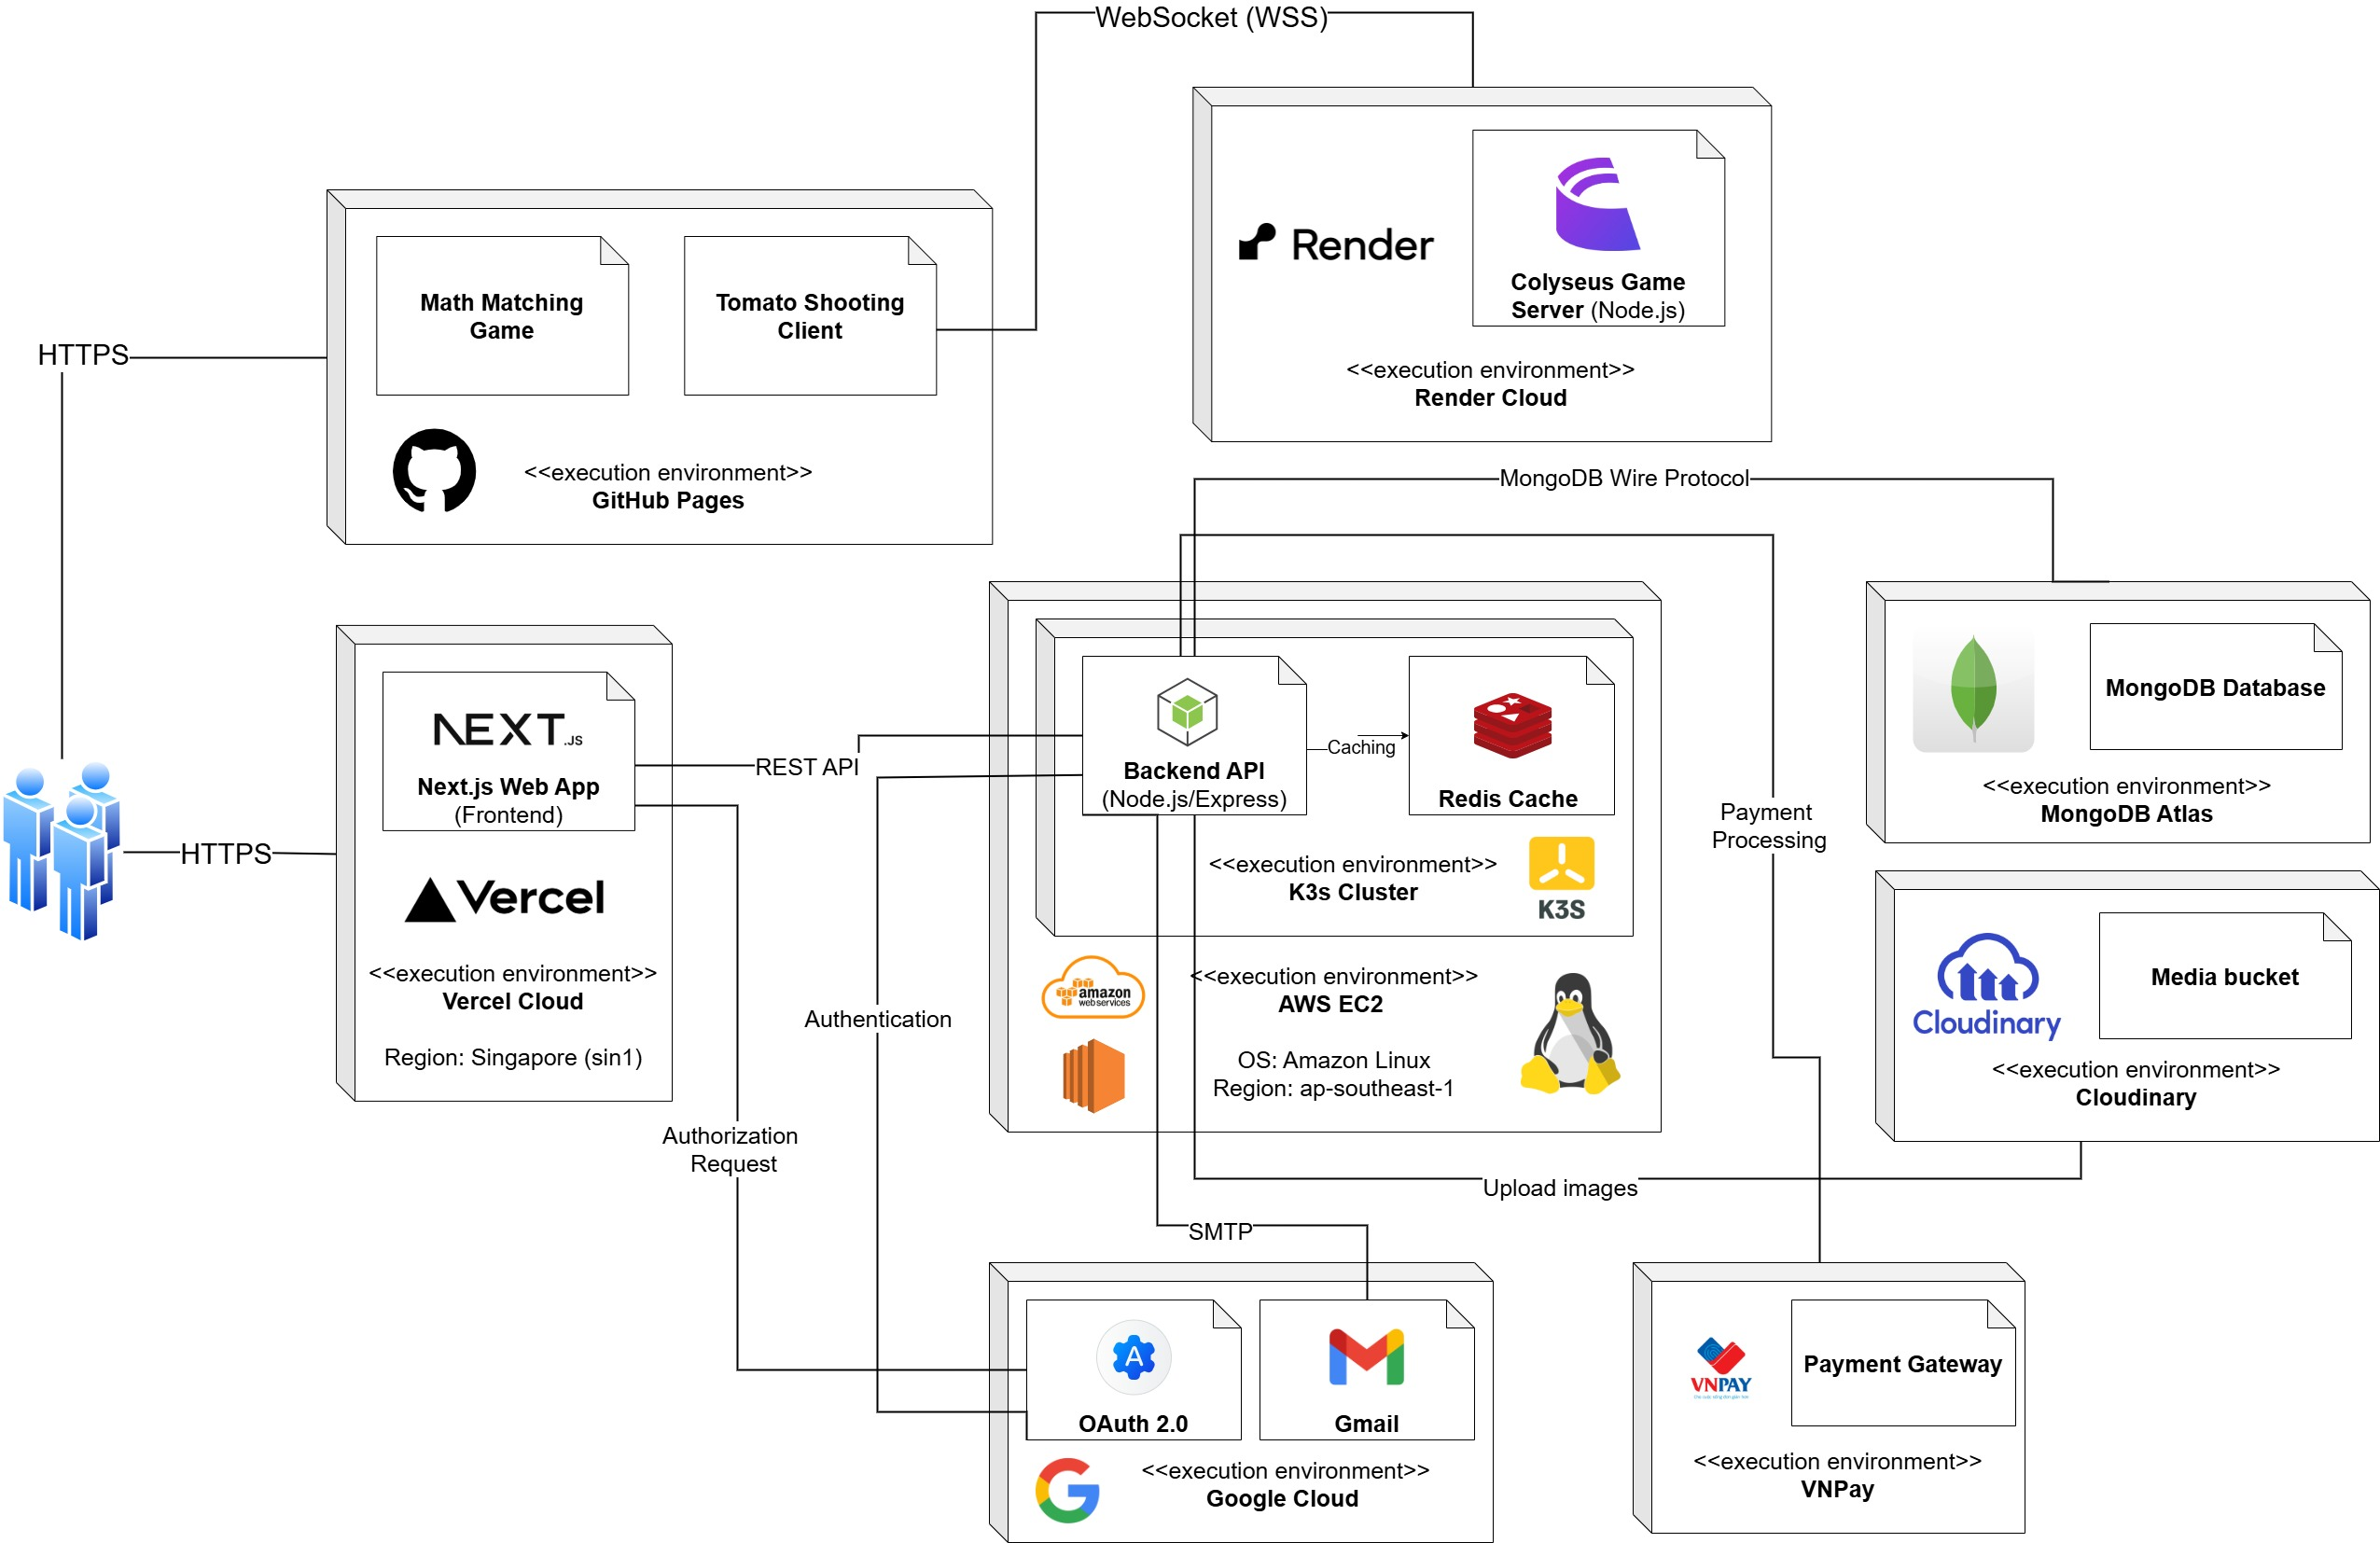
\includegraphics[width=1.0\textwidth]{Image/Deployment.jpg}
	\vspace{0.6cm}
	\caption{Landing Page}
	\label{fig:deploy}
\end{figure}

\subsubsection{Giao diện người dùng (Frontend)}
Giao diện người dùng được triển khai trên nền tảng điện toán đám mây Vercel được tối ưu hóa riêng cho Next.js và các ứng dụng full-stack hiện đại. Vercel hỗ trợ quy trình triển khai ứng dụng Next.js tối giản thông qua cơ chế CI/CD tự động từ kho lưu trữ Git. Vercel cung cấp mạng lưới Edge Network toàn cầu giúp tối ưu hóa tốc độ truy cập (latency), khả năng tự động mở rộng (auto-scaling) và tính năng Preview Deployments cho mỗi pull request.
\begin{itemize}
	\item \textbf{Các bước triển khai}:
	\begin{enumerate}
		\item Truy cập vào dashboard của Vercel và tạo project mới để triển khai.
		\item Import repository mã nguồn của frontend vào Vercel và liên kết với project mới vừa được tạo.
		\item Cấu hình các biến môi trường cần thiết.
		\item Cấu hình Ignored Build Step sử dụng Customized Command:
		\begin{verbatim}
			if [ "$VERCEL_GIT_COMMIT_REF" == "prod" ]; 
			then exit 1; 
			else exit 0; 
			fi
		\end{verbatim}
		Đoạn mã trên thiết lập cơ chế kiểm soát quá trình triển khai tự động (CI/CD), đảm bảo hệ thống chỉ thực hiện việc biên dịch và phát hành khi có thay đổi trên nhánh \textit{prod}. Các thay đổi trên những nhánh khác sẽ bị bỏ qua nhằm tối ưu hóa tài nguyên và thời gian triển khai.
	\end{enumerate}
	\item \textbf{Cấu hình Hạ tầng và Môi trường vận hành}
	\begin{itemize}
		\item \textbf{Môi trường Xây dựng (Build Environment):}
		\begin{itemize}
			\item \textbf{Tài nguyên:} 4 vCPU và 8 GB RAM.
			\item \textbf{Vai trò:} Chịu trách nhiệm cài đặt các thư viện phụ thuộc, biên dịch mã nguồn và đóng gói ứng dụng (build artifact) trước khi triển khai chính thức.
		\end{itemize}
		
		\item \textbf{Môi trường Thực thi (Runtime Environment):}
		\begin{itemize}
			\item \textbf{Tài nguyên:} 1 vCPU và 2 GB RAM.
			\item \textbf{Vai trò:} Xử lý các yêu cầu (requests) trực tiếp từ người dùng cuối thông qua cơ chế Serverless Functions của Vercel.
		\end{itemize}
		
		\item \textbf{Vị trí Địa lý (Region):}
		\begin{itemize}
			\item \textbf{Khu vực:} Singapore (\texttt{sin1}).
			\item \textbf{Đặc điểm:} Việc đặt máy chủ tại Singapore giúp tối ưu hóa tốc độ phản hồi, giảm thiểu độ trễ mạng (network latency) cho người dùng tại khu vực Việt Nam và Đông Nam Á.
		\end{itemize}
	\end{itemize}
\end{itemize}

\subsubsection{Backend}
\begin{itemize}
	\item \textbf{Tổng quan về môi trường triển khai:}
	AWS là nền tảng điện toán đám mây cung cấp hạ tầng mạnh mẽ, tạo điều kiện thuận lợi cho việc triển khai hệ thống container trên các máy ảo EC2. Giải pháp này cho phép vận hành ứng dụng theo mô hình Kubernetes tập trung, đảm bảo tính ổn định và khả năng mở rộng tối ưu.

	
	\begin{itemize}
		\item \textbf{Dịch vụ hạ tầng:} AWS EC2 (Elastic Compute Cloud).
		\item \textbf{Vị trí máy chủ (Region):} Singapore (\texttt{ap-southeast-1}).
		\item \textbf{Trạng thái:} Hệ thống đang hoạt động ổn định (Production Ready).
	\end{itemize}
	
	\item \textbf{Thông số kỹ thuật và Cấu hình hệ thống}
	
	\begin{enumerate}
		\item \textbf{Nền tảng điều phối và Môi trường thực thi:}
		Hệ thống áp dụng công nghệ Container hóa (Docker) và được điều phối bởi Kubernetes rút gọn (K3s), giúp tối ưu hóa tài nguyên trên máy chủ. K3s được lựa chọn nhờ kiến trúc tối giản, phù hợp với các instance EC2 có cấu hình vừa phải. Ngoài ra, K3s còn cho phép người dùng vận hành các công cụ chuẩn của Kubernetes như Deployment, Service và YAML manifest để quản lý vòng đời ứng dụng một cách nhất quán qua giao diện dòng lệnh \texttt{kubectl} \cite{k3s}.  Việc kết hợp K3s và AWS giúp tận dụng hạ tầng đàn hồi của EC2 trong khi vẫn giữ quyền kiểm soát toàn diện cụm (cluster). Giải pháp này đáp ứng tốt các yêu cầu về chi phí, hiệu năng và khả năng mở rộng quy mô trong môi trường thực tế.
		
		\begin{itemize}[leftmargin=*, label=\textbullet, topsep=0.3em]
			\item \textbf{Hệ điều hành:} Amazon Linux (Truy cập quản trị qua tài khoản
			\texttt{ec2-user}).
			\item \textbf{Nền tảng điều phối:} K3s (Lightweight Kubernetes).
			\item \textbf{Kiến trúc hệ thống:} \texttt{linux/amd64}.
			\item \textbf{Mô hình triển khai:} High Availability với 02 bản sao (Replicas)
			chạy song song.
		\end{itemize}
		
		\item \textbf{Định mức tài nguyên hệ thống (Resource Quotas)}
		Tài nguyên được phân bổ chi tiết cho mỗi đơn vị thực thi (Pod) nhằm đảm bảo
		hiệu suất ổn định:
		
		\vspace{0.5em}
		\begin{table}[ht] % Môi trường table giúp thêm caption và label
			\centering % Căn giữa bảng trên trang
			\begin{tabular}{lll}
				\toprule
				\textbf{Thông số} & \textbf{Mức yêu cầu (Request)} & \textbf{Mức giới hạn (Limit)} \\
				\midrule
				CPU               & 50m (0.05 Core)                & 200m (0.2 Core)               \\
				Bộ nhớ (RAM)      & 64 MiB                         & 256 MiB                       \\
				\bottomrule
			\end{tabular}
			\caption{Bảng định mức tài nguyên cho hệ thống} % Chú thích của bảng
			\label{tab:dinh-muc-tai-nguyen} % Nhãn để dùng lệnh \ref{} khi cần nhắc tới bảng trong bài
		\end{table}
		\vspace{0.5em}
		
		\item \textbf{Các thành phần dịch vụ tích hợp}
		
		\begin{itemize}[leftmargin=*, label=\textbullet, topsep=0.3em]
			\item \textbf{Cơ sở dữ liệu NoSQL:} MongoDB, kết nối thông qua chuỗi định
			danh (URI) được bảo mật.
			\item \textbf{Hệ thống Cache:} Redis, được triển khai trực tiếp bên trong
			cụm Kubernetes.
			\item \textbf{Lưu trữ tệp tin:} Cloudinary (Dịch vụ quản lý hình ảnh đám mây).
			\item \textbf{Cổng thanh toán:} VNPAY Sandbox (Môi trường thử nghiệm tích hợp).
		\end{itemize}
		
	\end{enumerate}
	
	\item \textbf{Quy trình triển khai kỹ thuật (Deployment Workflow)}
	Quy trình triển khai hệ thống được thực hiện một cách tuần tự qua các giai đoạn sau:
	
	\begin{itemize}
		\item \textbf{Giai đoạn 1 -- Đóng gói Ứng dụng:} Sử dụng Docker để xây dựng
		Image hệ thống hỗ trợ kiến trúc Linux/amd64, sau đó đẩy lên kho lưu trữ
		Docker Hub.
		\item \textbf{Giai đoạn 2 -- Chuyển giao cấu hình:} Sử dụng giao thức SCP để
		đồng bộ các tệp cấu hình Kubernetes (\texttt{.yaml}) từ môi trường phát
		triển lên máy chủ EC2.
		\item \textbf{Giai đoạn 3 -- Thực thi triển khai:} Kết nối SSH vào máy chủ để
		khởi tạo các tài khoản định danh (Secrets) và áp dụng cấu hình thông qua
		công cụ \texttt{kubectl}.
		\item \textbf{Giai đoạn 4 -- Kiểm tra và Giám sát:} Thực hiện kiểm tra trạng
		thái các Pod và dịch vụ K3s để xác nhận quá trình triển khai hoàn tất và
		không có lỗi phát sinh.
	\end{itemize}
	
	\item \textbf{Thiết lập Bảo mật Hạ tầng (AWS Security Group)}
	
	Để bảo vệ hệ thống trước các truy cập trái phép, quy tắc tường lửa (Security
	Group) được cấu hình nghiêm ngặt theo mô hình tối giản các cổng kết nối (Least
	Privilege):
	
	\vspace{0.5em}
	\begin{table}[ht]
		\centering
		\renewcommand{\arraystretch}{1.4} % Tăng khoảng cách dòng cho thoáng
		\begin{tabularx}{\textwidth}{l l l l X}
			\toprule
			\textbf{Loại lưu lượng} & \textbf{Giao thức} & \textbf{Cổng} & \textbf{Đối tượng} & \textbf{Mục đích} \\
			\midrule
			Bảo mật SSH & TCP & 22 & Quản trị viên & Truy cập dòng lệnh để quản lý và bảo trì server. \\
			Ứng dụng Web & TCP & 30081 & Công cộng & Tiếp nhận yêu cầu từ người dùng tới hệ thống Dino Math. \\
			\bottomrule
		\end{tabularx}
		\caption{Cấu hình lưu lượng mạng cho hệ thống}
	\end{table}
	\vspace{0.5em}
	
\end{itemize}

\subsubsection{Minigames}
\begin{itemize}
	\item \textbf{Minigame chơi đơn (Math Matching):}
	\begin{itemize}
		\item \textbf{Nền tảng triển khai:} GitHub Pages.
		\item \textbf{Cơ chế vận hành:} Tự động hóa quy trình build và deploy thông qua \textbf{GitHub Actions} ngay khi mã nguồn được cập nhật.
		\item \textbf{Ưu điểm:} Đảm bảo tính nhất quán, phát hành nhanh chóng và không tốn chi phí vận hành máy chủ tĩnh.
	\end{itemize}
	
	\item \textbf{Trò chơi đa người chơi (Tomato Shooting):}
	\begin{itemize}
		\item \textbf{Phần Game Client:} Triển khai tương tự trên \textbf{GitHub Pages} tích hợp \textbf{GitHub Actions} để tự động hóa quá trình phát hành phiên bản mới nhất.
		\item \textbf{Phần Máy chủ thời gian thực (Server):} Triển khai trên nền tảng \textbf{Render}. Render là nền tảng điện toán đám mây (PaaS) hỗ trợ triển khai ứng dụng web, API và các dịch vụ nền (background services) một cách đơn giản, tích hợp CI/CD tự động từ kho lưu trữ Git. Render được sử dụng để triển khai máy chủ \textbf{Colyseus} -- thành phần xử lý logic game đa người chơi thời gian thực. 
		\item \textbf{Ưu điểm của Render:} So với việc tự quản lý hạ tầng trên AWS, Render giúp đơn giản hóa đáng kể quy trình triển khai và vận hành server Colyseus: tự động build và deploy khi có commit mới lên nhánh chính, hỗ trợ WebSocket vốn là giao thức cốt lõi của Colyseus, và cung cấp logs theo thời gian thực để theo dõi trạng thái server trong quá trình phát triển. Ngoài ra, Render có gói miễn phí phù hợp với quy mô của đề tài, giúp tiết kiệm chi phí vận hành trong giai đoạn phát triển và demo.
		\item \textbf{Vai trò máy chủ:} Xử lý kết nối đa người chơi, đồng bộ trạng thái trận đấu và truyền tải dữ liệu thời gian thực với độ trễ thấp.
	\end{itemize}
\end{itemize}



% Cấu hình forest cho cây thư mục
\forestset{
  dir tree/.style={
    for tree={
      font=\ttfamily,
      grow'=0,
      child anchor=west,
      parent anchor=south,
      anchor=west,
      calign=first,
      edge path={
        \noexpand\path [draw, \forestoption{edge}]
        (!u.south west) +(7.5pt,0) |- node[fill,inner sep=1.25pt] {} (.child anchor)\forestoption{edge label};
      },
      before typesetting nodes={
        if n=1
          {insert before={[,phantom]}}
          {}
      },
      fit=band,
      before computing xy={l=15pt},
    }
  }
}

% Cấu hình listings
\lstset{
  basicstyle=\ttfamily\small,
  breaklines=true,
  frame=single,
  xleftmargin=2em,
  framexleftmargin=1.5em,
  backgroundcolor=\color{gray!10}
}
\subsection{Cấu trúc mã nguồn}

\subsubsection{Tổng quan cấu trúc mã nguồn}
\label{sec:tong-quan-ma-nguon}

Dự án \textbf{Dino Math} được thiết kế và phát triển dựa trên kiến trúc \textbf{Client-Server} phân lớp, nhằm đảm bảo tính độc lập giữa giao diện người dùng và logic xử lý nghiệp vụ. Mã nguồn của hệ thống được tổ chức thành hai thành phần chính, tương ứng với hai kho lưu trữ (repository) riêng biệt để thuận tiện cho việc quản lý phiên bản và triển khai độc lập:

\begin{itemize}
	\item \textbf{Phần giao diện người dùng (Frontend):} 
	Được xây dựng trên nền tảng framework \textit{Next.js} kết hợp với \textit{React} và ngôn ngữ \textit{TypeScript} nhằm đảm bảo tính chặt chẽ về kiểu dữ liệu và tối ưu hóa hiệu năng phía người dùng. Điểm đặc biệt của hệ thống là việc tích hợp trực tiếp game engine \textit{Cocos Creator}, cho phép vận hành các Minigame toán học tương tác một cách mượt mà ngay trên trình duyệt.
	
	\item \textbf{Phần xử lý trung tâm (Backend):} 
	Sử dụng môi trường thực thi \textit{Node.js} kết hợp với framework \textit{Express} và ngôn ngữ \textit{TypeScript}. Hệ thống quản trị dữ liệu thông qua cơ sở dữ liệu NoSQL \textit{MongoDB} để lưu trữ thông tin người dùng và kết quả học tập; đồng thời tích hợp \textit{Redis} làm bộ nhớ đệm (caching) nhằm tối ưu hóa tốc độ truy xuất và nâng cao khả năng phản hồi của hệ thống.
\end{itemize}

Sự kết hợp giữa các công nghệ hiện đại này không chỉ giúp dự án vận hành ổn định mà còn tạo tiền đề thuận lợi cho việc triển khai linh hoạt trên hạ tầng đám mây AWS \cite{awsec2} và quản lý thông qua cụm k3s \cite{k3s}.

\vspace{0.5cm}

\textbf{Cấu trúc thư mục tổng quan:}

\begin{forest}
  dir tree
  [dino-math-project/
    [dino-fe/ \textit{(Frontend - Next.js)}
      [src/
        [apis/ \textit{(API clients)}]
        [app/ \textit{(Routes)}]
        [components/ \textit{(UI)}]
        [stores/ \textit{(State)}]
        [types/ \textit{(TypeScript)}]
      ]
      [public/
        [assets/ \textit{(Images)}]
        [web-desktop/ \textit{(Cocos build)}]
      ]
    ]
    [dino\_math\_backend/ \textit{(Backend - Express)}
      [src/ \textit{(Source)}
        [controllers/ \textit{(Logic)}]
        [model/ \textit{(Schemas)}]
        [routes/ \textit{(Endpoints)}]
        [middleware/ \textit{(Auth)}]
      ]
      [ERD/ \textit{(DB design)}]
    ]
  ]
\end{forest}

\subsubsection{Cấu trúc Frontend}

\subsubsubsection{Tổng quan Frontend}

Frontend được xây dựng trên \textbf{Next.js 14} với App Router, sử dụng TypeScript và Zustand cho state management. Hệ thống tích hợp Cocos Creator để render các bài tập tương tác.

\begin{forest}
  dir tree
  [dino-fe/
    [src/
      [apis/]
      [app/]
      [components/]
      [stores/]
      [types/]
    ]
    [public/
      [assets/]
      [web-desktop/ \textit{(Cocos Creator build)}
    ]
    [eslint.config.mjs]
    [next.config.ts]
    [package.json]
    [tsconfig.json]
  ]
\end{forest}

\subsubsubsection{Thư mục \texttt{app/} - Routes}

Các route chính của ứng dụng sử dụng App Router với Route Groups:

\textbf{Route Groups:}
\begin{itemize}
\item \texttt{(full)} -- Layout fullscreen không có navbar, dùng cho adventure và arena-exam
\item \texttt{(main)} -- Layout chuẩn có navbar, dùng cho home, lessons, arena, v.v.
\end{itemize}

\textbf{Dynamic Routes:}
\begin{itemize}
\item \texttt{[gradeLevel]} -- Khối lớp động (1, 2, 3, ...)
\item \texttt{[topicId]} -- ID chủ đề động
\end{itemize}

\subsubsubsection{Thư mục \texttt{components/} - UI Components}


\textbf{Các components chính:}
\begin{itemize}
\item \texttt{GameComponent/} -- Cocos game integration
\item \texttt{Navbar/} -- Navigation bar cho layout (main)
\item \texttt{ProfilePopup/} -- Avatar selection popup
\item \texttt{Loader/}, \texttt{ScreenLoader/} -- Loading states
\item \texttt{RoundedTextBox/}, \texttt{RoundedPasswordBox/} -- Form inputs
\item \texttt{OTPInput/} -- OTP verification
\item \texttt{LectureSlider/} -- Lesson navigation
\item \texttt{MascotWriting/} -- Animated mascot
\item \texttt{Volume/} -- Audio control
\end{itemize}

\subsubsubsection{Thư mục \texttt{apis/} - API Clients}

\begin{forest}
  dir tree
  [apis/
    [authApis.ts]
    [config.ts]
    [index.ts]
    [lessonApis.ts]
    [userApis.ts]
    [worldApis.ts]
  ]
\end{forest}

\textbf{Nội dung:}
\begin{itemize}
\item \texttt{authApis.ts} -- Authentication API calls (login, register, logout)
\item \texttt{config.ts} -- API base URL và configuration
\item \texttt{index.ts} -- Export tất cả API functions
\item \texttt{lessonApis.ts} -- Lesson/lecture/exercise API calls
\item \texttt{userApis.ts} -- User profile và management APIs
\item \texttt{worldApis.ts} -- World/grade/land data APIs
\end{itemize}

\subsubsubsection{Thư mục \texttt{stores/} - State Management}

Quản lý state toàn cục với Zustand:

\begin{forest}
  dir tree
  [stores/
    [lessonStore.ts]
    [userStore.ts]
  ]
\end{forest}

\textbf{Stores:}
\begin{itemize}
\item \texttt{lessonStore.ts} -- Current lesson state, exercises, progress
\item \texttt{userStore.ts} -- User information, authentication state
\end{itemize}

\subsubsubsection{Thư mục \texttt{types/} - TypeScript Types}

\begin{forest}
  dir tree
  [types/
    [dto.types.ts]
    [index.ts]
  ]
\end{forest}

\textbf{Types:}
\begin{itemize}
\item \texttt{dto.types.ts} -- Data Transfer Objects (API request/response types)
\item \texttt{index.ts} -- Export tất cả types
\end{itemize}

\subsubsubsection{Thư mục \texttt{public/} - Static Assets}

\begin{forest}
  dir tree
  [public/
    [assets/
      [arena/]
      [auth/]
      [exercises/]
      [games/]
      [home/]
      [landing/]
      [leaderboard/]
      [mission/]
      [onboarding/]
    ]
    [web-desktop/ \textit{(Cocos Creator build)}
      [application.js]
      [index.html]
      [index.js]
      [style.css]
      [assets/
        [internal/]
        [main/]
        [resources/]
      ]
      [cocos-js/]
      [src/]
    ]
  ]
\end{forest}

\textbf{Nội dung:}
\begin{itemize}
\item \texttt{assets/} -- Hình ảnh, icons, SVG theo từng module
\item \texttt{web-desktop/} -- Build output của Cocos Creator game engine
  \begin{itemize}
  \item \texttt{assets/main/} -- Game assets (sprites, animations, JSON configs)
  \item \texttt{cocos-js/} -- Cocos engine runtime
  \item \texttt{src/} -- Game source bundles
  \end{itemize}
\end{itemize}

\subsubsection{Module Frontend}

\subsubsubsection{Module Xác thực (Auth)}

\textbf{Cấu trúc:}

\begin{forest}
  dir tree
  [app/auth/
    [page.tsx \textit{(Login/Register)}]
    [reset-password/
      [page.tsx]
    ]
  ]
\end{forest}

\textbf{Chức năng:}
\begin{itemize}
\item Xác thực người dùng
\item Lưu trữ và làm mới JWT token
\item Phân quyền theo vai trò (student, parent, admin)
\item Reset password qua email/OTP
\end{itemize}

\subsubsubsection{Module Học sinh (Student Dashboard)}

\textbf{Cấu trúc:}

\begin{forest}
  dir tree
  [app/student/
    [(main)/
      [layout.tsx]
      [home/ \textit{(Dashboard)}]
      [lessons/ \textit{(Browse)}]
      [arena/ \textit{(Compete)}]
      [leaderboard/ \textit{(Ranking)}]
      [missions/ \textit{(Quests)}]
      [games/ \textit{(Minigames)}]
      [history/ \textit{(Progress)}]
    ]
    [(full)/
      [adventure/ \textit{(Learning)}]
      [arena-exam/ \textit{(Testing)}]
    ]
  ]
\end{forest}

\textbf{Chức năng:}
\begin{itemize}
\item Hiển thị bài học khả dụng
\item Theo dõi tiến độ
\item Xem điểm số và thành tích
\item Thi đấu và xếp hạng
\end{itemize}

\subsubsubsection{Module Cocos Game Integration}

\textbf{Cấu trúc:}

\begin{forest}
  dir tree
  [components/GameComponent/
    [CocosComponent.tsx \textit{(Core bridge)}]
    [CocosGameWrapper.tsx \textit{(React wrapper)}]
  ]
\end{forest}

\textbf{Chức năng:}
\begin{itemize}
\item Tích hợp Cocos Creator vào React
\item Render 6 dạng bài tập:
  \begin{itemize}
  \item Kéo thả (Drag \& Drop)
  \item Điền từ (Fill in the blank)
  \item Ghép đôi (Matching)
  \item Trắc nghiệm (Multiple Choice)
  \item Đúng/Sai (True/False)
  \item Phân loại chẵn lẻ (Odd/even classification)

  \end{itemize}
\item Bridge communication giữa React và Cocos
\item Quản lý lifecycle của game instance
\end{itemize}

\textbf{Luồng hoạt động:}
\begin{enumerate}
\item Component nhận props chứa dữ liệu bài tập từ API
\item CocosGameWrapper khởi tạo engine
\item Serialize và truyền data vào game
\item Học sinh tương tác trong Cocos canvas
\item Kết quả gửi ngược về React
\item Cập nhật state và gọi API lưu tiến độ
\end{enumerate}

\newpage
\subsubsubsection{Module Arena (Đấu trường)}

\textbf{Cấu trúc:}

\begin{forest}
  dir tree
  [app/student/
    [(main)/arena/ \textit{(Browse mode)}
      [page.tsx]
      [ArenaClient.tsx]
    ]
    [(full)/arena-exam/ \textit{(Exam mode)}
      [page.tsx]
      [ExamClient.tsx]
    ]
  ]
\end{forest}

\textbf{Chức năng:}
\begin{itemize}
\item Thi trắc nghiệm có giới hạn thời gian
\item Xếp hạng và so sánh điểm
\item Xem lại đáp án
\end{itemize}

\subsubsubsection{Data Flow Frontend}

\begin{enumerate}
\item UI Component nhận user interaction
\item Component gọi Store action hoặc API service
\item Store xử lý logic và gọi API
\item API trả dữ liệu về
\item Store cập nhật state
\item UI re-render
\end{enumerate}

\subsubsection{Cấu trúc Backend}

\subsubsubsection{Tổng quan Backend}

Backend được xây dựng trên \textbf{Node.js + Express + TypeScript}, kết nối \textbf{MongoDB} (database) và \textbf{Redis} (cache/session). API theo chuẩn RESTful với Swagger documentation.

\begin{forest}
  dir tree
  [dino\_math\_backend/
    [src/]
    [ERD/]
    [sample\_data-main/]
    [docker-compose.yml]
    [Dockerfile]
    [package.json]
    [tsconfig.json]
  ]
\end{forest}

\subsubsubsection{Thư mục \texttt{src/} - Source Code}

Kiến trúc MVC:

\begin{forest}
  dir tree
  [src/
    [index.ts]
    [controllers/]
    [middleware/]
    [model/]
    [routes/]
    [utils/]
  ]
\end{forest}

\subsubsubsection{Thư mục \texttt{controllers/}}

\begin{forest}
  dir tree
  [controllers/
    [auth.controller.ts]
    [user.controller.ts]
    [lesson.controller.ts]
    [lecture.controller.ts]
    [exercise.controller.ts]
    [arena.controller.ts]
    [participation.controller.ts]
    [grade.controller.ts]
    [world.controller.ts]
    [land.controller.ts]
    [rank.controller.ts]
    [academicTerm.controller.ts]
  ]
\end{forest}

\textbf{Mô tả:}
\begin{itemize}
\item \texttt{auth.controller.ts} -- Authentication
\item \texttt{user.controller.ts} -- User management
\item Các controllers khác xử lý business logic cho từng resource
\end{itemize}

\subsubsubsection{Thư mục \texttt{model/} - Database Schemas}

\begin{forest}
  dir tree
  [model/
    [user.ts]
    [family.ts]
    [lesson.ts]
    [lecture.ts]
    [exercise.ts]
    [arena.ts]
    [participation.ts]
    [grade.ts]
    [world.ts]
    [land.ts]
    [rank.ts]
    [academicTerm.ts]
  ]
\end{forest}

\textbf{Mô tả:}
\begin{itemize}
\item \texttt{user.ts} -- User schema
\item \texttt{family.ts} -- Family \& invite codes
\item \texttt{participation.ts} -- Exam results
\item Các schemas khác định nghĩa cấu trúc dữ liệu MongoDB
\end{itemize}

\subsubsubsection{Thư mục \texttt{routes/} - API Endpoints}

\begin{forest}
  dir tree
  [routes/
    [auth.routes.ts]
    [user.routes.ts]
    [lesson.routes.ts]
    [lecture.routes.ts]
    [exercise.routes.ts]
    [arena.routes.ts]
    [participation.routes.ts]
    [grade.routes.ts]
    [world.routes.ts]
    [land.routes.ts]
    [rank.routes.ts]
    [academicTerm.routes.ts]
  ]
\end{forest}

\textbf{Endpoints chính:}
\begin{itemize}
\item \texttt{auth.routes.ts} -- /auth/register, /auth/login
\item \texttt{user.routes.ts} -- CRUD /users
\item Các routes khác định nghĩa CRUD endpoints
\end{itemize}

\subsubsubsection{Thư mục \texttt{middleware/}}

\begin{forest}
  dir tree
  [middleware/
    [auth.middleware.ts]
    [logger.ts]
    [rateLimit.ts]
  ]
\end{forest}

\textbf{Middleware:}
\begin{itemize}
\item \texttt{auth.middleware.ts} -- JWT verification
\item \texttt{logger.ts} -- Request logging
\item \texttt{rateLimit.ts} -- Rate limiting
\end{itemize}

\subsubsubsection{Thư mục \texttt{utils/}}

\begin{forest}
  dir tree
  [utils/
    [redisClient.ts]
    [swagger.ts]
  ]
\end{forest}

\textbf{Utilities:}
\begin{itemize}
\item \texttt{redisClient.ts} -- Redis singleton
\item \texttt{swagger.ts} -- API docs config
\end{itemize}

\subsubsection{Module Backend}

\subsubsubsection{Module Authentication}

\textbf{Files:} \texttt{auth.controller.ts}, \texttt{auth.middleware.ts}, \texttt{user.ts}, \texttt{family.ts}

\textbf{Chức năng:}
\begin{itemize}
\item \textbf{Đăng ký (POST /auth/register):}
  \begin{itemize}
  \item Validate email và password strength
  \item Hash password với bcrypt
  \item Tạo Family và inviteCode cho parent
  \item Lưu user vào MongoDB
  \end{itemize}
  
\item \textbf{Đăng nhập (POST /auth/login):}
  \begin{itemize}
  \item Verify credentials
  \item Generate JWT tokens
  \item Lưu token vào Redis với TTL
  \item Trả về token + user info
  \end{itemize}
  
\item \textbf{Middleware:}
  \begin{itemize}
  \item Kiểm tra Bearer token
  \item Verify JWT signature
  \item Check token trong Redis
  \item Inject user info vào request
  \end{itemize}
  
\item \textbf{Đăng xuất (POST /auth/logout):}
  \begin{itemize}
  \item Xóa token khỏi Redis
  \item Invalidate session
  \end{itemize}
\end{itemize}

\subsubsubsection{Module User Management}

\textbf{Files:} \texttt{user.controller.ts}, \texttt{user.ts}

\textbf{API Endpoints:}
\begin{itemize}
\item \texttt{GET /users} -- Danh sách users (admin)
\item \texttt{GET /users/:id} -- Chi tiết user
\item \texttt{PUT /users/:id} -- Cập nhật profile
\item \texttt{DELETE /users/:id} -- Xóa user (admin)
\end{itemize}

\textbf{Phân quyền:}
\begin{itemize}
\item \textbf{Admin:} Toàn quyền
\item \textbf{Parent:} Xem chính mình và members trong family
\item \textbf{Student:} Chỉ xem chính mình và family members
\end{itemize}

\subsubsubsection{Module Lesson \& Lecture}

\textbf{Files:} \texttt{lesson.controller.ts}, \texttt{lecture.controller.ts}

\textbf{Kiến trúc phân cấp:}
\begin{enumerate}
\item \textbf{Grade} -- Khối lớp (Lớp 1, 2, ...)
\item \textbf{Lesson} -- Bài học (thuộc Grade + AcademicTerm)
\item \textbf{Lecture} -- Bài giảng (chi tiết nội dung)
\item \textbf{Exercise} -- Bài tập thực hành
\end{enumerate}

\textbf{API Endpoints:}
\begin{itemize}
\item \texttt{GET /lessons} -- Filter theo grade, subject, term
\item \texttt{GET /lessons/:id} -- Chi tiết + populate lectures
\item \texttt{POST /lessons} -- Tạo mới
\item \texttt{PUT /lessons/:id} -- Cập nhật
\item \texttt{DELETE /lessons/:id} -- Xóa
\end{itemize}

\subsubsubsection{Module Exercise}

\textbf{Files:} \texttt{exercise.controller.ts}, \texttt{exercise.ts}

\textbf{Chức năng:}
\begin{itemize}
\item 6 dạng bài tập:
  \begin{itemize}
  \item Multiple Choice
  \item True/False
  \item Fill in the Blank
  \item Drag \& Drop
  \item Matching
  \item Odd/even classification
  \end{itemize}
\item Gắn với lecture cụ thể
\item Lưu đáp án và điểm số
\item Hỗ trợ multimedia
\end{itemize}

\textbf{API Endpoints:}
\begin{itemize}
\item \texttt{GET /exercises} -- Filter theo lectureId
\item \texttt{GET /exercises/:id} -- Chi tiết
\item \texttt{POST /exercises} -- Tạo mới
\item \texttt{PUT /exercises/:id} -- Cập nhật
\item \texttt{DELETE /exercises/:id} -- Xóa
\end{itemize}

\subsubsubsection{Module Arena}

\textbf{Files:} \texttt{arena.controller.ts}, \texttt{participation.controller.ts}

\textbf{Chức năng:}
\begin{itemize}
\item Tạo đề thi với time limit
\item Chọn câu hỏi từ exercise pool
\item Tracking qua Participation model
\item Tính battlePoints và xếp hạng
\item 3 loại arena:
  \begin{itemize}
  \item Practice Mode
  \item Exam Mode
  \item Competition Mode
  \end{itemize}
\end{itemize}

\textbf{API Endpoints:}
\begin{itemize}
\item \texttt{GET /arenas} -- Danh sách
\item \texttt{POST /arenas} -- Tạo mới
\item \texttt{GET /arenas/:id/start} -- Bắt đầu làm bài
\item \texttt{POST /participations/:id/submit} -- Nộp bài
\item \texttt{GET /participations/:id/result} -- Xem kết quả
\end{itemize}

\subsubsubsection{Module Rank}

\textbf{Files:} \texttt{rank.controller.ts}, \texttt{rank.ts}

\textbf{Chức năng:}
\begin{itemize}
\item Định nghĩa cấp bậc (Bronze, Silver, Gold, ...)
\item Điều kiện thăng hạng theo battlePoints
\item Phần thưởng (quartz, avatars, ...)
\end{itemize}

\subsubsection{Data Flow Hệ thống}

\subsubsubsection{Luồng Đăng nhập}

\begin{enumerate}
\item Client: POST \texttt{/auth/login} (email + password)
\item Backend: Verify credentials với MongoDB
\item Backend: Generate JWT token
\item Backend: Lưu token vào Redis (TTL 7 days)
\item Backend: Trả token + user info
\item Client: Lưu token vào localStorage
\item Các request sau: Gửi token qua Authorization header
\end{enumerate}

\subsubsubsection{Luồng Làm bài tập}

\begin{enumerate}
\item Client: GET \texttt{/lessons/:id}
\item Backend: Trả lesson + populate lectures
\item Client: GET \texttt{/exercises?lectureId=xxx}
\item Backend: Trả exercises
\item Client: Render trong Cocos wrapper
\item Học sinh làm bài
\item Client: Gửi kết quả
\item Backend: Lưu Participation + cập nhật progress
\end{enumerate}

\subsubsubsection{Luồng Arena (Thi đấu)}

\begin{enumerate}
\item Client: GET \texttt{/arenas} -- Lấy danh sách
\item Client: GET \texttt{/arenas/:id/start}
\item Backend: Tạo Participation (status="in\_progress")
\item Backend: Trả exerciseIds + startTime
\item Client: Hiển thị câu hỏi + timer
\item Client: POST \texttt{/participations/:id/submit}
\item Backend:
  \begin{itemize}
  \item Validate timeLimit
  \item Chấm điểm
  \item Cập nhật battlePoints
  \item Check và update rank
  \item Update participation (completed)
  \end{itemize}
\item Client: Hiển thị kết quả + leaderboard
\end{enumerate}

\subsubsection{Kết luận}
Cấu trúc mã nguồn của dự án \textbf{Dino Math} được tổ chức một cách khoa học và nhất quán theo mô hình phân lớp. Việc tách biệt hoàn toàn giữa các thành phần không chỉ giúp nhóm phát triển dễ dàng quản lý mã nguồn mà còn tối ưu hóa quy trình kiểm thử và triển khai độc lập. Toàn bộ mã nguồn của dự án hiện được lưu trữ công khai nhằm phục vụ mục đích kiểm tra và phát triển, cụ thể tại các kho lưu trữ: \href{https://github.com/coldwind444/dino-fe.git}{Frontend Repository} và \href{https://github.com/boyastro/dino_math_backend.git}{Backend Repository}. Cách tiếp cận này đảm bảo hệ thống có khả năng mở rộng cao, sẵn sàng cho việc tích hợp thêm các tính năng giáo dục phức tạp mà không làm ảnh hưởng đến độ ổn định cốt lõi của ứng dụng.


% Chuong 7
\newpage
\section{Kiểm thử}

Toàn bộ mã nguồn và kết quả kiểm thử được công khai tại:
\url{https://github.com/khoa9894/Light-House}.

\subsection{Kiểm thử hiệu năng giao diện}

\subsubsection{Tổng quan}

Nhóm đã tiến hành kiểm thử giao diện người dùng bằng công cụ Google Lighthouse
trên tổng cộng \textbf{26 trang}, bao gồm \textbf{14 trang Admin Panel} và
\textbf{12 trang Main Web}. Các chỉ số được đo gồm: \textbf{Performance (P)},
\textbf{Accessibility (A)}, \textbf{Best Practices (BP)} và \textbf{SEO (S)}
trên thang điểm 0--100.

Nhìn chung, kết quả kiểm thử cho thấy phần lớn các trang đạt điểm tương đối
tốt ở hầu hết các hạng mục. Tuy nhiên, vẫn còn một số điểm cần cải thiện,
đặc biệt ở hạng mục Accessibility và một số chỉ số Performance trên các
trang có tương tác phức tạp.

% --------------------------------------------------------
\subsubsection{Kết quả Admin Panel}

\begin{longtable}{lp{5cm}cccc}
\toprule
\textbf{Trang} & \textbf{URL} & \textbf{P} & \textbf{A} & \textbf{BP} & \textbf{S} \\
\midrule
\endfirsthead
\toprule
\textbf{Trang} & \textbf{URL} & \textbf{P} & \textbf{A} & \textbf{BP} & \textbf{S} \\
\midrule
\endhead
\bottomrule
\endfoot

Accounts
  & /dashboard/accounts
  & \scoreGreen{99}  & \scoreOrange{83} & \scoreGreen{100} & \scoreGreen{100} \\
\rowcolor{lhrowgray}
Arenas
  & /dashboard/study/arenas
  & \scoreGreen{100} & \scoreOrange{84} & \scoreGreen{100} & \scoreGreen{100} \\
Exercises
  & /dashboard/study/lessons/.../exercises
  & \scoreGreen{100} & \scoreOrange{83} & \scoreGreen{100} & \scoreGreen{100} \\
\rowcolor{lhrowgray}
Games
  & /dashboard/minigames
  & \scoreOrange{93} & \scoreOrange{84} & \scoreGreen{100} & \scoreGreen{100} \\
Grades
  & /dashboard/study/grades
  & \scoreGreen{100} & \scoreOrange{89} & \scoreGreen{100} & \scoreGreen{100} \\
\rowcolor{lhrowgray}
Lessons
  & /dashboard/study/lessons
  & \scoreGreen{100} & \scoreOrange{84} & \scoreGreen{100} & \scoreGreen{100} \\
Login
  & /auth/login
  & \scoreGreen{100} & \scoreGreen{98}  & \scoreGreen{100} & \scoreOrange{92} \\
\rowcolor{lhrowgray}
Register
  & /auth/register
  & \scoreGreen{100} & \scoreGreen{98}  & \scoreGreen{100} & \scoreOrange{92} \\
Root
  & /
  & \scoreGreen{100} & \scoreOrange{93} & \scoreGreen{100} & \scoreOrange{92} \\
\rowcolor{lhrowgray}
Semester
  & /dashboard/study/semesters
  & \scoreGreen{100} & \scoreOrange{84} & \scoreGreen{100} & \scoreGreen{100} \\
Tasks
  & /dashboard/tasks
  & \scoreGreen{100} & \scoreOrange{85} & \scoreGreen{100} & \scoreGreen{100} \\
\rowcolor{lhrowgray}
Tests
  & /dashboard/study/tests
  & \scoreGreen{100} & \scoreOrange{83} & \scoreGreen{100} & \scoreGreen{100} \\
Theory
  & /dashboard/study/.../theory
  & \scoreGreen{100} & \scoreOrange{81} & \scoreGreen{100} & \scoreGreen{100} \\
\rowcolor{lhrowgray}
Topics
  & /dashboard/study/topics
  & \scoreOrange{97} & \scoreOrange{84} & \scoreGreen{100} & \scoreGreen{100} \\

\bottomrule
\caption{Điểm Lighthouse --- Admin Panel}
\label{tab:lighthouse-admin}
\end{longtable}

\textbf{Nhận xét:}
\begin{itemize}[leftmargin=*]
  \item \textbf{Performance:} 12/14 trang Admin đạt điểm Performance từ 99--100.
        Hai trang còn lại (Games và Topics) đạt 93 và 97, vẫn nằm trong ngưỡng chấp
        nhận được. Điều này cho thấy việc tối ưu bundle size và lazy loading đã được
        thực hiện ở mức cơ bản.
  \item \textbf{Best Practices:} Toàn bộ 14/14 trang đạt \textbf{100/100}, cho thấy
        code nhìn chung tuân thủ các quy chuẩn kỹ thuật hiện đại.
  \item \textbf{SEO:} 11/14 trang đạt 100. Ba trang Login, Register và Root đạt 92 ---
        đây là mức chấp nhận được vì Admin Panel không đặt ưu tiên SEO cao.
  \item \textbf{Accessibility:} Đây là hạng mục có điểm thấp nhất, dao động từ 81 đến
        98. Một số trang chưa đáp ứng đầy đủ các tiêu chuẩn hỗ trợ người dùng khuyết
        tật, và đây là điểm cần cải thiện trong các phiên bản tiếp theo.
\end{itemize}

% --------------------------------------------------------
\subsubsection{Kết quả Main Web}

\begin{longtable}{lp{5cm}cccc}
\toprule
\textbf{Trang} & \textbf{URL} & \textbf{P} & \textbf{A} & \textbf{BP} & \textbf{S} \\
\midrule
\endfirsthead
\toprule
\textbf{Trang} & \textbf{URL} & \textbf{P} & \textbf{A} & \textbf{BP} & \textbf{S} \\
\midrule
\endhead
\bottomrule
\endfoot

Arena
  & /student/arena
  & \scoreOrange{96} & \scoreGreen{94}  & \scoreOrange{96} & \scoreGreen{100} \\
\rowcolor{lhrowgray}
Auth
  & /auth
  & \scoreGreen{99}  & \scoreGreen{94}  & \scoreGreen{100} & \scoreOrange{92} \\
Games
  & /student/games
  & \scoreOrange{94} & \scoreGreen{94}  & \scoreGreen{100} & \scoreGreen{100} \\
\rowcolor{lhrowgray}
History
  & /student/history
  & \scoreOrange{97} & \scoreOrange{84} & \scoreGreen{100} & \scoreGreen{100} \\
Home
  & /student/home
  & \scoreOrange{98} & \scoreGreen{96}  & \scoreGreen{100} & \scoreGreen{100} \\
\rowcolor{lhrowgray}
Landing
  & /
  & \scoreGreen{100} & \scoreGreen{94}  & \scoreGreen{100} & \scoreOrange{92} \\
Leaderboard
  & /student/leaderboard
  & \scoreOrange{97} & \scoreOrange{93} & \scoreGreen{100} & \scoreGreen{100} \\
\rowcolor{lhrowgray}
Milestones
  & /student/adventure/...
  & \scoreOrange{93} & \scoreOrange{89} & \scoreGreen{100} & \scoreGreen{100} \\
Mission
  & /student/missions
  & \scoreGreen{99}  & \scoreGreen{96}  & \scoreGreen{100} & \scoreGreen{100} \\
\rowcolor{lhrowgray}
ParentDashboard
  & /parent/dashboard
  & \scoreOrange{97} & \scoreOrange{84} & \scoreGreen{100} & \scoreGreen{100} \\
ResetPassword
  & /auth/reset-password
  & \scoreGreen{100} & \scoreOrange{90} & \scoreGreen{100} & \scoreOrange{92} \\
\rowcolor{lhrowgray}
Topics
  & /student/lessons
  & \scoreOrange{93} & \scoreOrange{89} & \scoreGreen{100} & \scoreGreen{100} \\

\bottomrule
\caption{Điểm Lighthouse --- Main Web}
\label{tab:lighthouse-mainweb}
\end{longtable}

\textbf{Nhận xét:}
\begin{itemize}[leftmargin=*]
  \item \textbf{Accessibility:} Điểm Accessibility của Main Web (trung bình khoảng 92)
        nhìn chung cao hơn Admin Panel (trung bình khoảng 87). Điều này có thể do giao
        diện người dùng cuối được chú ý hơn trong quá trình phát triển, dù vẫn còn
        dư địa để cải thiện.
  \item \textbf{Best Practices:} 11/12 trang đạt 100. Trang Arena đạt 96 do một số
        tính năng tương tác thời gian thực ảnh hưởng nhỏ đến chỉ số này.
  \item \textbf{Performance:} Không có trang nào dưới 93 --- hầu hết các trang đã
        được tối ưu ở mức cơ bản và không gặp vấn đề nghiêm trọng về tốc độ tải.
  \item \textbf{SEO:} Ba trang Auth, Landing và ResetPassword đạt 92 do cấu hình
        \texttt{robots.txt} chưa hoàn chỉnh; đây là điểm cần xử lý trong thời gian tới.
\end{itemize}

% --------------------------------------------------------
\subsubsection{Các vấn đề phát hiện và hướng khắc phục}

Qua quá trình kiểm thử, nhóm ghi nhận một số vấn đề còn tồn tại:

\begin{enumerate}[leftmargin=*]
  \item \textbf{Thiếu thẻ \texttt{<main>} (document landmark)} --- Nhiều trang chưa
        có thẻ \texttt{<main>} bao quanh nội dung chính, ảnh hưởng đến khả năng
        điều hướng của screen reader. Đây là cải tiến đơn giản, có thể thực hiện
        trong thời gian ngắn.
  \item \textbf{Tương phản màu sắc chưa đủ} --- Một số cặp màu chữ/nền chưa đạt tỉ
        lệ tương phản 4.5:1 theo tiêu chuẩn WCAG AA, làm giảm điểm Accessibility
        trên nhiều trang.
  \item \textbf{Render-blocking requests} --- Một số tài nguyên CSS/JS chặn quá trình
        render ban đầu; có thể cải thiện bằng cách inline critical CSS hoặc dùng
        thuộc tính \texttt{rel="preload"}.
  \item \textbf{JavaScript chưa được tree-shaking triệt để} --- Bundle size còn có thể
        giảm thêm thông qua tối ưu code splitting và loại bỏ code không sử dụng.
  \item \textbf{File \texttt{robots.txt} chưa hợp lệ} --- Cần cấu hình lại để tránh
        ảnh hưởng đến điểm SEO của các trang công khai.
\end{enumerate}

% --------------------------------------------------------
\subsubsection{Đánh giá chung}

Nhìn chung, kết quả kiểm thử Lighthouse cho thấy hệ thống đạt mức hiệu năng
chấp nhận được so với quy mô của một đồ án sinh viên. Hạng mục Best Practices
đạt tốt trên hầu hết các trang, trong khi Performance và SEO ở mức khá. Tuy
nhiên, điểm Accessibility vẫn còn thấp ở một số trang và cần được ưu tiên cải
thiện trong các phiên bản tiếp theo, đặc biệt với đối tượng người dùng là học
sinh tiểu học --- nhóm cần giao diện thân thiện và dễ tiếp cận.

Các vấn đề phát hiện được nhìn chung đều có hướng khắc phục rõ ràng và không
đòi hỏi thay đổi kiến trúc lớn, do đó có thể được xử lý dần trong quá trình
bảo trì và phát triển tiếp theo của dự án.

% ======================================================
\subsection{Kiểm thử tự động (Playwright)}

\subsubsection{Tổng quan}

Nhóm đã thực hiện kiểm thử tự động bằng \textbf{Playwright} thông qua file
\texttt{arena.spec.ts}, chạy song song trên \textbf{5 browser/project}:
\textit{auth, chromium, edge, firefox, webkit}.

\begin{center}
\begin{tabular}{lcccccc}
\toprule
\textbf{Browser} & \textbf{Tổng} & \textbf{Pass} & \textbf{Fail} & \textbf{Skip} & \textbf{Flaky} & \textbf{Tỉ lệ} \\
\midrule
auth     & 38  & \scoreGreen{38}  & 0 & 0 & 0 & \scoreGreen{100\%} \\
\rowcolor{lhrowgray}
chromium & 51  & \scoreGreen{51}  & 0 & 0 & 0 & \scoreGreen{100\%} \\
edge     & 51  & \scoreGreen{51}  & 0 & 0 & 0 & \scoreGreen{100\%} \\
\rowcolor{lhrowgray}
firefox  & 51  & \scoreGreen{51}  & 0 & 0 & 0 & \scoreGreen{100\%} \\
webkit   & 11  & \scoreGreen{11}  & 0 & 0 & 0 & \scoreGreen{100\%} \\
\midrule
\textbf{Tổng} & \textbf{202} & \textbf{\textcolor{lhgreen}{202}} & \textbf{0} & \textbf{0} & \textbf{0} & \scoreGreen{\textbf{100\%}} \\
\bottomrule
\end{tabular}
\end{center}

\vspace{0.5em}
\noindent Kết quả tổng hợp: \textbf{202/202 test cases passed}, không có test nào
failed hoặc flaky trên toàn bộ các browser được kiểm thử.

% --------------------------------------------------------
\subsubsection{Chi tiết các nhóm test cases}

Tổng cộng \textbf{89 test cases độc lập} được phân thành 14 nhóm chức năng:

\begin{longtable}{clccc}
\toprule
\textbf{Nhóm} & \textbf{Chức năng} & \textbf{Cases} & \textbf{Thời gian TB} & \textbf{Kết quả} \\
\midrule
\endfirsthead
\toprule
\textbf{Nhóm} & \textbf{Chức năng} & \textbf{Cases} & \textbf{Thời gian TB} & \textbf{Kết quả} \\
\midrule
\endhead
\bottomrule
\endfoot

TC-01 & Login                      & 10 & 5.6s  & \scoreGreen{PASS} \\
\rowcolor{lhrowgray}
TC-02 & Register                   & 17 & 3.1s  & \scoreGreen{PASS} \\
TC-03 & Home (Student)             & 5  & 11.5s & \scoreGreen{PASS} \\
\rowcolor{lhrowgray}
TC-04 & Topics / Lessons           & 5  & 13.7s & \scoreGreen{PASS} \\
TC-05 & Milestones                 & 4  & 12.8s & \scoreGreen{PASS} \\
\rowcolor{lhrowgray}
TC-06 & Arena / Assessment         & 6  & 8.9s  & \scoreGreen{PASS} \\
TC-07 & Claim Rewards              & 1  & 20.0s & \scoreGreen{PASS} \\
\rowcolor{lhrowgray}
TC-08 & History (Student + Parent) & 13 & 7.0s  & \scoreGreen{PASS} \\
TC-09 & Leaderboard                & 3  & 5.6s  & \scoreGreen{PASS} \\
\rowcolor{lhrowgray}
TC-10 & Games                      & 3  & 7.2s  & \scoreGreen{PASS} \\
TC-11 & Reset Password             & 6  & 13.4s & \scoreGreen{PASS} \\
\rowcolor{lhrowgray}
TC-12 & Register Profile           & 5  & 8.3s  & \scoreGreen{PASS} \\
TC-13 & Forgot Password            & 5  & 14.6s & \scoreGreen{PASS} \\
\rowcolor{lhrowgray}
TC-14 & Edit Profile               & 6  & 9.6s  & \scoreGreen{PASS} \\

\bottomrule
\caption{Chi tiết test cases theo nhóm chức năng}
\label{tab:playwright}
\end{longtable}

% --------------------------------------------------------
\subsubsection{Nhận xét kiểm thử tự động}

\begin{itemize}[leftmargin=*]
  \item \textbf{Tỉ lệ pass:} 202/202 test cases passed trên cả 5 browser, trong đó
        webkit (Safari engine) thường có độ tương thích thấp hơn các browser khác nhưng
        vẫn cho kết quả tốt trong lần kiểm thử này.
  \item \textbf{Không có flaky test:} Toàn bộ test cases cho kết quả ổn định qua
        nhiều lần chạy, không có trường hợp kết quả không nhất quán do timing.
  \item \textbf{Phạm vi bao phủ:} 14 nhóm test cases bao gồm các luồng chính của
        hệ thống: xác thực, nội dung học tập, đấu trường, lịch sử, bảng xếp hạng,
        trò chơi và quản lý tài khoản.
  \item \textbf{Kiểm thử biên:} Các nhóm TC-01 và TC-02 bao gồm cả trường hợp
        input không hợp lệ (rỗng, sai định dạng, trùng lặp) bên cạnh luồng chính.
  \item \textbf{Hạn chế:} Phạm vi kiểm thử hiện tập trung vào giao diện người dùng
        cuối; các luồng của Admin Panel chưa được bao phủ bởi kiểm thử tự động và
        có thể được bổ sung trong các giai đoạn tiếp theo.
\end{itemize}



% Chuong 8
\newpage
\section{Tổng kết}
\subsection{Kết quả giai đoạn 1}
Sau khi kết thúc giai đoạn 1, nhóm chúng em đã xác định được phạm vi cũng như các yêu cầu cần thiết của hệ thống. Hệ thống được thiết kế hướng đến việc nâng cao trải nghiệm học tập và tạo động lực học toán cho học sinh tiểu học thông qua các tính năng tương tác, game hóa và theo dõi tiến độ học tập chi tiết.

\newline
\vspace{0.2cm}
Sau khi kết thúc giai đoạn 1, nhóm đã hoàn thành được các công việc sau đây:
\begin{enumerate}
	\item Xác định được phạm vi và yêu cầu của hệ thống cho phù hợp với nhu cầu sử dụng của người dùng hiện tại, cụ thể là học sinh ở cấp bậc Tiểu học và phụ huynh có con em đang học tập tại cấp bậc này. 
	\item Thiết kế được cơ sở dữ liệu để đáp ứng được các yêu cầu lưu trữ của hệ thống.
	\item Thiết kế giao diện người dùng trên nền tảng web và đặt ra các tiêu chí để đánh giá giao diện, bao gồm: thân thiện với người dùng, sáng tạo, độc đáo, thu hút người dùng và đáp ứng được các yêu cầu nghiệp vụ của hệ thống. Các giao diện bao gồm:
	\begin{itemize}
		\item \textbf{Đối với học sinh:} Trang chủ, trang bài học, trang chủ đề, trang đấu trường, trang bài tập, trang bài thi, trang xếp hạng, trang nhiệm vụ, trang minigames, trang lịch sử làm bài, giao diện quản lý tài khoản cá nhân bao gồm cập nhật thông tin cá nhân (ảnh đại diện, tên, lớp), đổi mật khẩu, liên kết tài khoản. 
		\item \textbf{Đối với phụ huynh:} Trang chủ, trang thống kê tổng quan, trang lịch sử làm bài, trang minigames, giao diện quản lý tài khoản cá nhân bao gồm cập nhật thông tin cá nhân (ảnh đại diện, lớp), đổi mật khẩu, liên kết tài khoản, nâng cấp tài khoản.
	\end{itemize}
	\item Thiết kế và hiện thực được một số dạng bài tập tương tác (mục \ref{subsec:interact}).
	\item Hiện thực được 1 minigame là Math Match.
	\item Hiện thực được các API cơ bản: 
	\begin{itemize}
		\item Đăng nhập, đăng ký tài khoản.
		\item Quản lý hồ sơ người dùng (xem và cập nhật thông tin cá nhân).
		\item Cập nhật tiến độ học tập.
		\item Cập nhật điểm tích tích lũy (thạch anh) cho người dùng.
		\item Lấy các dữ liệu về khối lớp, thế giới và các vùng đất liên quan, chủ đề, bài học, bài tập dạng tương tác.
	\end{itemize}
	\item Hiện thực được các logic ở frontend như sau:
	\begin{itemize}
		\item Đăng nhập, đăng ký tài khoản.
		\item Cập nhật thông tin học sinh trên trang Onboarding (mục \ref{subsec:onboarding}), nâng cao sự gắn kết giữa người dùng và hệ thống.
		\item Cập nhật thông tin người dùng (ảnh đại diện, họ và tên, khối lớp).
		\item Tích hợp được các dạng bài tập tương tác vào giao diện, đồng thời hoàn thành luồng làm bài tập cơ bản bao gồm: 
		\newline 
		Chọn lớp $\rightarrow$ Chọn chủ đề $\rightarrow$ Chọn bài học Làm bài $\rightarrow$ Xem kết quả
	\end{itemize}
\end{enumerate}

\subsection{Kế hoạch và phân công công việc giai đoạn 1}

\renewcommand{\arraystretch}{1.3}

\begin{longtable}{|>{\centering\arraybackslash}m{1.5cm}|m{7cm}|m{5cm}|}
	\hline
	\textbf{Tuần} & \textbf{Công việc} & \textbf{Người thực hiện} \\
	\hline
	\endfirsthead
	
	\hline
	\textbf{Tuần} & \textbf{Công việc} & \textbf{Người thực hiện} \\
	\hline
	\endhead
	
	\hline
	\endfoot
	
	38-39 & Xác định phạm vi đề tài: xây dựng website học toán tư duy cho học sinh tiểu học & Nguyễn Văn Thành \\
	\cline{2-3}
	& Xác định đối tượng người dùng, stakeholders và hệ thống liên quan & Trương Anh Khoa \\
	\cline{2-3}
	& Thống nhất yêu cầu người dùng và các chức năng cần thiết & Nguyễn Văn Thành, \newline Nguyễn Minh Tân, \newline Trương Anh Khoa \\
	\cline{2-3}
	& Thiết kế giao diện người dùng: Trang Landing, Trang chủ (học sinh), Trang Bài học và giao diện popup quản lý tài khoản người dùng. & Nguyễn Minh Tân \\
	\hline
	
	40-41 & Vẽ usecase diagram cho toàn bộ hệ thống và activity diagram cho các luồng Đăng nhập, Đăng ký, Làm bài tập. & Trương Anh Khoa \\
	\cline{2-3}
	& Vẽ sequence diagram cho các luồng Đăng nhập, Đăng ký, Làm bài tập. & Nguyễn Minh Tân \\
	\cline{2-3}
	& Thiết kế cơ sở dữ liệu. & Nguyễn Văn Thành \\
	\cline{2-3}
	& Thiết kế giao diện người dùng: Trang Milestone, Trang Đấu trường, Bảng xếp hạng, Trang Nhiệm vụ, Trang Làm bài kiểm tra. & Nguyễn Minh Tân \\
	\hline
	
	42-43 & Thiết kế kiến trúc hệ thống (Frontend – Backend – Database) & Nguyễn Văn Thành \\
	\cline{2-3}
	& Tạo các repository để quản lý mã nguồn cho frontend và backend & Nguyễn Văn Thành, \newline Nguyễn Minh Tân, \newline Trương Anh Khoa \\
	\cline{2-3}
	& Thiết kế giao diện người dùng: Trang Minigame, Trang Thống kê (phụ huynh), Trang Lịch sử làm bài & Nguyễn Minh Tân \\
	\hline
	
	44-45 & Setup backend, cấu hình server, tạo database và các bảng chính & Nguyễn Văn Thành \\
	\cline{2-3}
	& Hiện thực giao diện người dùng: Trang Landing, Trang chủ (học sinh), Trang Đấu trường, Trang Đăng nhập/Đăng ký, Trang Onboarding, Trang Milestone, Trang Lấy lại mật khẩu. & Nguyễn Minh Tân \\
	\cline{2-3}
	& Hiện thực giao diện người dùng: Trang Bài học, Trang Nhiệm vụ, Trang Bảng xếp hạng, giao diện quản lý tài khoản người dùng bao gồm Chỉnh sửa thông tin cá nhân, Đổi mật khẩu, Liên kết tài khoản. & Trương Anh Khoa \\
	\cline{2-3}
	& Hiện thực các API đăng nhập, đăng ký, lấy danh sách các chủ đề theo lớp. & Nguyễn Văn Thành \\
	\hline
	
	46-47 & Thiết kế các dạng bài tập tương tác (nối, đúng/sai, tô màu, kéo thả, điền khuyết) & Trương Anh Khoa \\
	\cline{2-3}
	& Hiện thực các dạng bài tập tương tác. & Trương Anh Khoa \\
	\cline{2-3}
	& Hoàn thiện và nối API cho chức năng đăng nhập và đăng ký tài khoản. & Nguyễn Minh Tân \\
	\cline{2-3}
	& Hiện thực các API quản lý khối lớp, chủ đề, bài tập, cập nhật điểm, quản lý tiến trình học tập & Nguyễn Văn Thành \\
	\hline
	
	48-49 & Hoàn thiện luồng làm bài tập tương tác ở frontend. & Nguyễn Minh Tân, \newline Trương Anh Khoa \\
	\cline{2-3}
	& Thiết kế và hoàn thiện minigame Math Match. & Trương Anh Khoa \\
	\cline{2-3}
	& Hiện thực các API quản lý tài khoản người dùng, gợi ý chủ đề học tập theo thời gian, quản lý đấu trường & Nguyễn Văn Thành \\
	\hline
	
	50-51 & Tối ưu backend, fix bugs, refactor code & Nguyễn Văn Thành \\
	\cline{2-3}
	& Hoàn thiện và nối API cho các chức năng quản lý tài khoản người dùng & Trương Anh Khoa \\
	\cline{2-3}
	& Hoàn thiện và nối API cho các chức năng chơi minigame, hiển thị tiến trình học tập & Nguyễn Minh Tân \\
	\cline{2-3}
	& Kiểm tra lại các chức năng cơ bản đã được hiện thực & Nguyễn Văn Thành, \newline Nguyễn Minh Tân, \newline Trương Anh Khoa \\
	\hline
	
\end{longtable}

\begin{figure}[H]
	\centering
	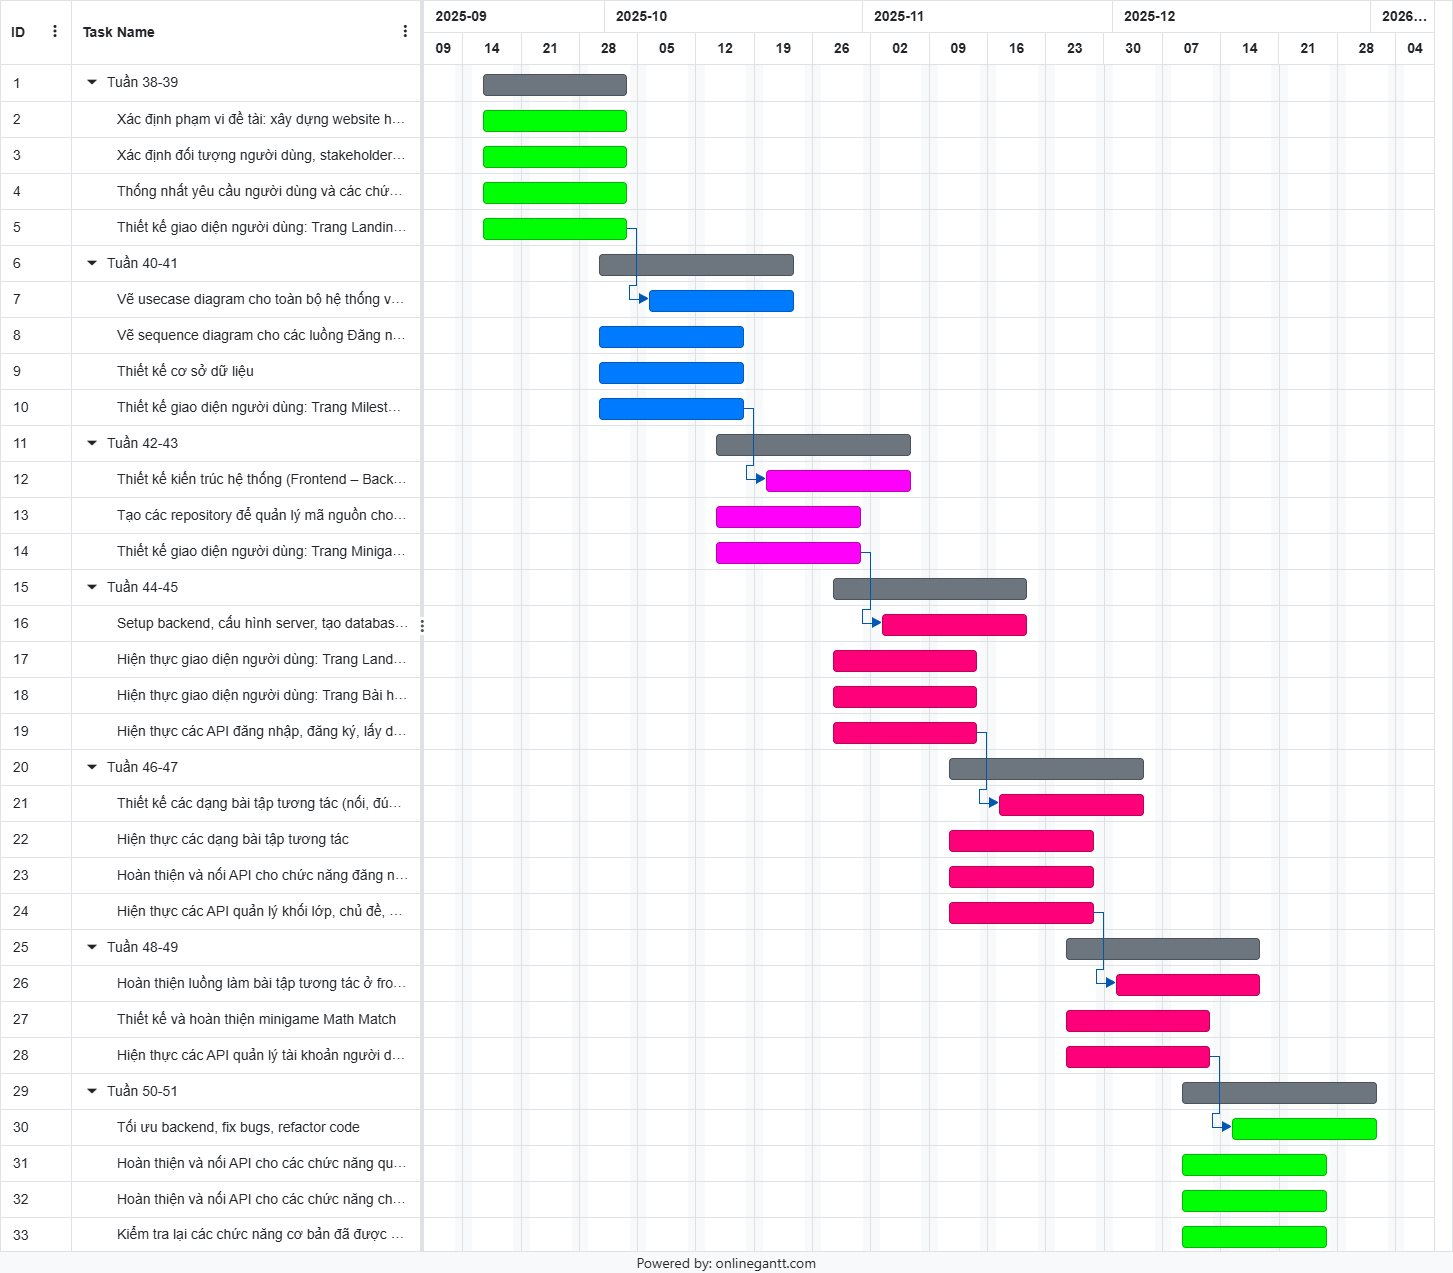
\includegraphics[width=\textwidth]{Image/phase1.jpg}
	\vspace{0.5cm}
	\caption{Biểu đồ Gantt giai đoạn 1}
	\label{fig:gantt-phase1}
\end{figure}


\newpage
\subsection{Kế hoạch và phân công công việc giai đoạn 2}
\renewcommand{\arraystretch}{1.3}
\begin{longtable}{|>{\centering\arraybackslash}m{2cm}|p{7.5cm}|p{4.5cm}|}
	\hline
	\textbf{Tuần} & \textbf{Công việc (Chi tiết thực hiện)} & \textbf{Người thực hiện} \\
	\hline
	\endfirsthead
	
	\hline
	\textbf{Tuần} & \textbf{Công việc (Chi tiết thực hiện)} & \textbf{Người thực hiện} \\
	\hline
	\endhead
	
	\hline
	\endfoot
	
	Tuần 1--2 & \textbf{Khởi động \& Triển khai tính năng Assessment cơ bản:} 
	
	\textbullet\ \textbf{BE:} Thiết kế cấu trúc cơ sở dữ liệu (Schema) cho Assessment, AssessmentResult và Answer. Xây dựng hệ thống API CRUD hoàn chỉnh để tạo, liệt kê và xem chi tiết bài kiểm tra. Thiết lập môi trường Swagger và chuẩn bị dữ liệu mẫu (Seed data). 
	
	\textbullet\ \textbf{FE:} Xây dựng giao diện danh sách các bài kiểm tra hiện có. Thiết kế trang chi tiết bài kiểm tra bao gồm mô tả, yêu cầu và thông tin tổng quan. Kết nối dữ liệu từ API để hiển thị lên giao diện. Hiện thực logic nghiệp vụ cho tính năng Đấu trường.
	
	\textbullet\ \textbf{Game:} Nghiên cứu và thiết kế bộ bài tập bám sát chương trình học của bộ Giáo dục và Đào tạo. & BE: Nguyễn Văn Thành
	
	FE: Nguyễn Minh Tân
	
	Game: Trương Anh Khoa \\
	\hline
	
	Tuần 3--4 & \textbf{Nộp bài \& Quy trình chấm điểm tự động:} 
	
	\textbullet\ \textbf{BE:} Hoàn thiện logic xử lý khi người dùng nộp bài (POST /submit). Xây dựng bộ máy chấm điểm tự động (Auto-grading) cho trắc nghiệm và đúng/sai. Viết unit test và tích hợp để kiểm tra luồng dữ liệu từ lúc nộp đến khi lưu điểm. 
	
	\textbullet\ \textbf{FE:} Phát triển giao diện làm bài trực tuyến (Quiz Interface). Tích hợp logic bộ đếm ngược thời gian và trình quản lý trạng thái câu trả lời (State Management). Xây dựng màn hình hiển thị kết quả bài thi ngay sau khi nộp. 
	
	\textbullet\ \textbf{Game:} Nghiên cứu các dạng bài tập tương tác. Thiết kế các assets và hiệu ứng hình ảnh tương ứng. & BE: Nguyễn Văn Thành
	
	FE: Nguyễn Minh Tân
	
	Game: Trương Anh Khoa \\
	\hline
	
	Tuần 5--6 & \textbf{Mission \& Achievement (Nhiệm vụ \& Thành tựu):} 
	
	\textbullet\ \textbf{BE:} Thiết kế Model Mission và Achievement. Xây dựng logic tự động cập nhật tiến trình (Progress) dựa trên hành động của người dùng (ví dụ: hoàn thành bài học, đăng nhập hàng ngày). API quản lý danh sách thành tựu người dùng đạt được. 
	
	\textbullet\ \textbf{FE:} Xây dựng Dashboard nhiệm vụ tập trung. Hiển thị danh sách nhiệm vụ hàng ngày/tuần kèm thanh tiến trình trực quan. Thiết kế trang hồ sơ cá nhân hiển thị kho huy hiệu thành tựu. 
	
	\textbullet\ \textbf{Game:} Xây dựng tính năng xem trước câu hỏi bài tập cho admin. & BE: Nguyễn Văn Thành
	
	FE: Nguyễn Minh Tân
	
	Game: Trương Anh Khoa \\
	\hline
	
	Tuần 7--8 & \textbf{RewardRecord \& Cơ chế thưởng:} 
	
	\textbullet\ \textbf{BE:} Triển khai Model RewardRecord để quản lý lịch sử biến động phần thưởng (Quartz, BP). Đảm bảo tính atomicity (giao dịch an toàn) khi cộng thưởng vào ví người dùng. Xác thực nguồn gốc phần thưởng để tránh lỗi dữ liệu. 
	
	\textbullet\ \textbf{FE:} Xây dựng giao diện admin quản lý người dùng, bao gồm danh sách tài khoản, chức năng tìm kiếm, lọc theo vai trò và khóa/mở khóa tài khoản. Thiết kế trang thống kê tổng quan cho admin.
	
	\textbullet\ \textbf{Game:} Nghiên cứu minigame tương tác 2 người thông qua server. & BE: Nguyễn Văn Thành
	
	FE: Nguyễn Minh Tân
	
	Game: Trương Anh Khoa \\
	\hline
	
	Tuần 9--10 & \textbf{FamilyGame \& FamilyReport (Tính năng gia đình):} 
	
	\textbullet\ \textbf{BE:} Xây dựng logic cho FamilyGame và tham gia nhóm. Thiết lập thuật toán tổng hợp dữ liệu để sinh báo cáo gia đình (FamilyReport), tính toán hiệu suất học tập trung bình của cả nhóm. 
	
	\textbullet\ \textbf{FE:} Thiết kế giao diện báo cáo gia đình với các biểu đồ so sánh (sử dụng thư viện biểu đồ). Xây dựng sảnh chờ (Lobby) cho các thành viên gia đình tương tác. 
	
	\textbullet\ \textbf{Game:} Phát triển logic và giao diện cho mini-game thi đấu giữa các thành viên. Đảm bảo tính đồng bộ dữ liệu điểm số trong thời gian thực. & BE: Nguyễn Văn Thành
	
	FE: Nguyễn Minh Tân
	
	Game: Trương Anh Khoa \\
	\hline
	
	Tuần 11--12 & \textbf{LectureResult \& ExerciseResult (Lưu trữ chi tiết):} 
	
	\textbullet\ \textbf{BE:} Tích hợp logic lưu trữ điểm số chi tiết cho từng bài giảng và từng bài tập nhỏ. Xây dựng API truy vấn lịch sử học tập sâu (theo từng bài học cụ thể) để phục vụ việc phân tích dữ liệu. 
	
	\textbullet\ \textbf{FE:} Xây dựng trang "Nhật ký học tập" chi tiết. Cho phép người dùng xem lại các bài tập đã làm sai để ôn tập lại. Cập nhật luồng UX khi người dùng kết thúc một bài giảng. & BE: Nguyễn Văn Thành
	
	FE: Nguyễn Minh Tân \\
	\hline
	
	Tuần 13--14 & \textbf{AI Recommendation \& Hoàn thiện hệ thống:} 
	
	\textbullet\ \textbf{AI \& BE:} Triển khai thuật toán gợi ý bài học dựa trên lịch sử làm bài (sai chủ đề nào gợi ý chủ đề đó) và sở thích cá nhân. Tối ưu hóa bảo mật API, cập nhật tài liệu Swagger toàn diện và chuẩn bị môi trường triển khai (Deploy). 
	
	\textbullet\ \textbf{FE:} Tích hợp khu vực "Gợi ý thông minh từ AI" vào trang chủ. Thực hiện Polish (tinh chỉnh) toàn bộ giao diện, sửa lỗi UI/UX tồn đọng sau các đợt kiểm thử. 
	
	\textbullet\ \textbf{Game:} Kiểm tra lại toàn bộ hiệu suất (Performance) của phần game, đảm bảo chạy mượt mà trên các thiết bị khác nhau. Đóng gói tài nguyên game. & BE: Nguyễn Văn Thành
	
	FE: Nguyễn Minh Tân
	
	Game: Trương Anh Khoa \\
	\hline
	
\end{longtable}

\begin{figure}[H]
	\centering
	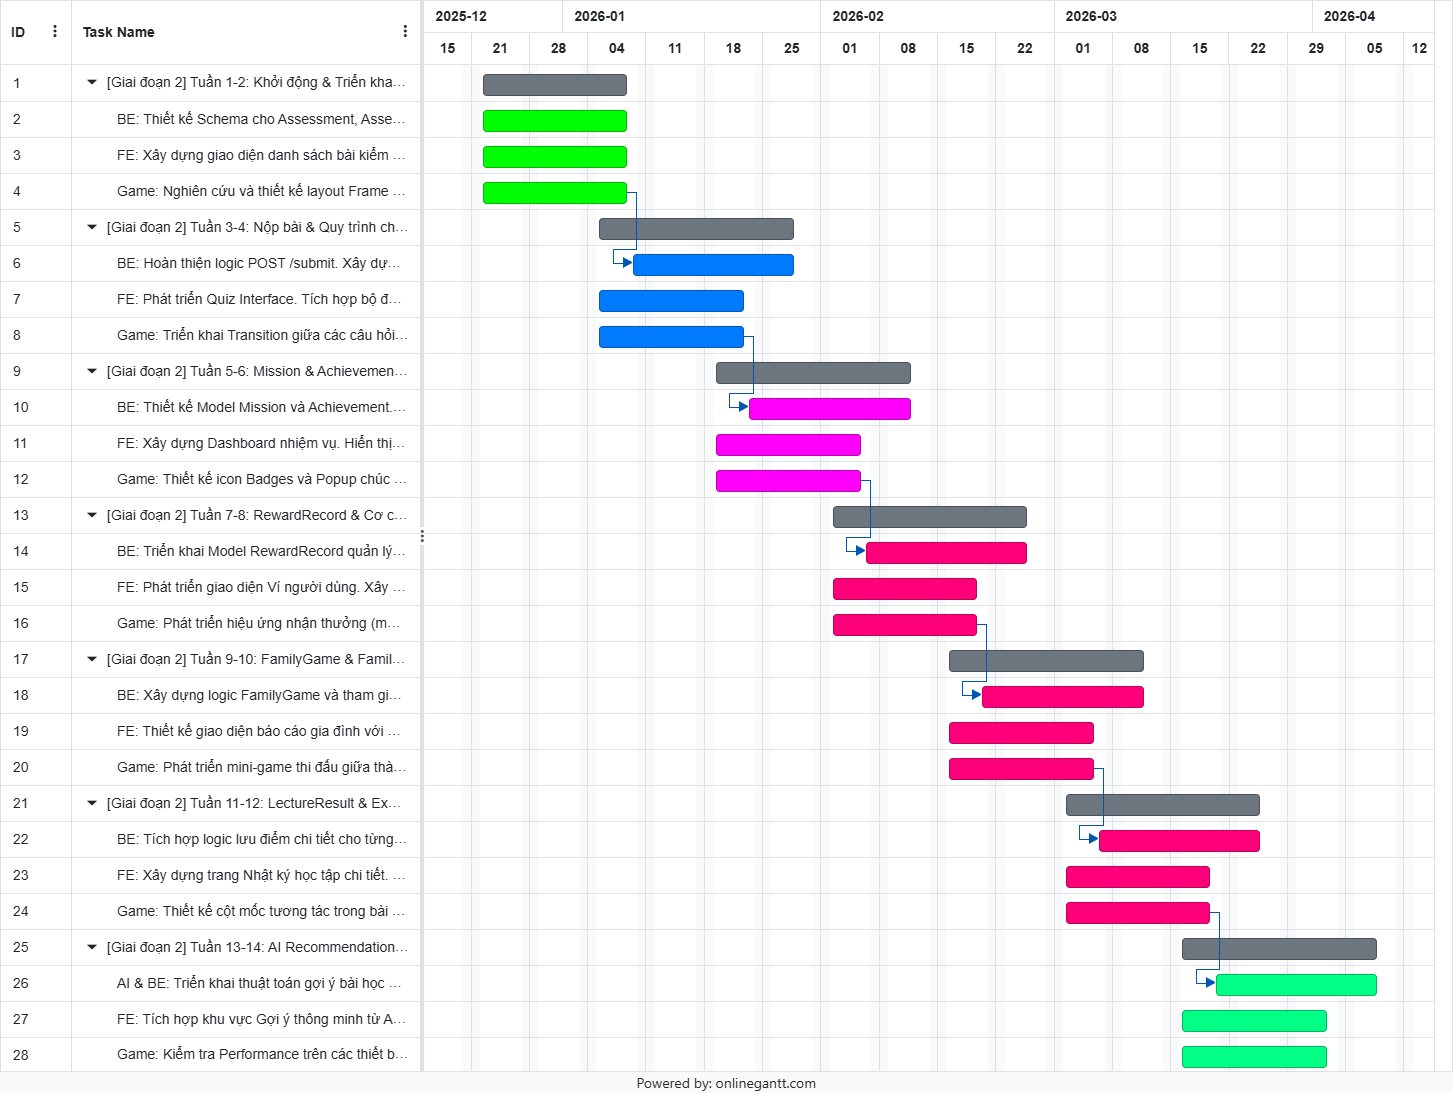
\includegraphics[width=\textwidth]{Image/phase2.jpg}
	\vspace{0.5cm}
	\caption{Biểu đồ Gantt giai đoạn 2}
	\label{fig:gantt-phase2}
\end{figure}

\subsection{Kết quả giai đoạn 2}
Sau khi kết thúc giai đoạn 2, nhóm đã hoàn thiện được các công việc sau đây:
\begin{enumerate}
	\item Hoàn thiện hệ thống bài kiểm tra (Assessment), bao gồm luồng làm bài trực tuyến, bộ đếm ngược thời gian, chấm điểm tự động và hiển thị kết quả.
	\item Hoàn thiện cơ chế nhiệm vụ (Mission) và thành tựu (Achievement), tự động cập nhật tiến trình dựa trên hành động của người dùng.
	\item Hoàn thiện hệ thống phần thưởng (RewardRecord) quản lý lịch sử biến động điểm thưởng của người dùng.
	\item Xây dựng đầy đủ giao diện và chức năng quản trị hệ thống (Admin), bao gồm:
	\begin{itemize}
		\item Quản lý tài khoản người dùng (tìm kiếm, lọc theo vai trò, khóa/mở khóa tài khoản).
		\item Trang thống kê tổng quan hệ thống.
	\end{itemize}
	\item Hiện thực được \textbf{18 dạng toán tương tác} phục vụ học sinh luyện tập bám sát chương trình của Bộ Giáo dục và Đào tạo.
	\item Hiện thực được \textbf{1 minigame} đơn người chơi.
	\item Hiện thực được \textbf{1 game tương tác 2 người} theo thời gian thực.
	\item Lưu trữ chi tiết kết quả học tập (LectureResult, ExerciseResult), hỗ trợ người dùng xem lại lịch sử và các bài tập đã làm sai.
	\item Hoàn thiện báo cáo gia đình (FamilyReport) với các biểu đồ so sánh hiệu suất học tập giữa các thành viên.
\end{enumerate}

\vspace{0.3cm}
\noindent\textbf{Hạn chế còn tồn đọng:} Nhóm chưa hoàn thành được tính năng tích hợp AI để tự động sinh bài tập theo trình độ người dùng. Đây sẽ là hướng phát triển tiếp theo của hệ thống trong tương lai.



\newpage
\clearpage
\phantomsection
\renewcommand{\refname}{Tài liệu tham khảo}
\addcontentsline{toc}{section}{Tài liệu tham khảo}

\begin{thebibliography}{99}
	
	\bibitem{bogddt2018}
	Bộ Giáo dục và Đào tạo,
	\textit{Chương trình Giáo dục phổ thông - Chương trình môn Toán (Ban hành kèm theo Thông tư số 32/2018/TT-BGDĐT)},
	https://vanban.chinhphu.vn/?pageid=27160&docid=215347,
	2018.
	
	\bibitem{cocoscreator38}
	Cocos Technologies, 
	\textit{Cocos Creator 3.8 User Manual},  
	https://docs.cocos.com/creator/3.8/manual/en/,  
	Truy cập ngày 15/10/2025.
	
	\bibitem{leong2015concrete}
	Leong, Y. H., Ho, W. K., \& Cheng, L. P.,
	\textit{Concrete-Pictorial-Abstract: Surveying its Origins and Charting its Future},
	The Mathematics Enthusiast, Vol. 12, 2015.
	
	\bibitem{chou2015}
	Yu-kai Chou,
	\textit{Actionable Gamification: Beyond Points, Badges, and Leaderboards},
	Octalysis Media, 2015.
	
	\bibitem{k3s}
	Rancher Labs,  
	\textit{K3s Documentation},  
	https://docs.k3s.io/,  
	Truy cập ngày 10/10/2025.
	
	\bibitem{nodejs}
	OpenJS Foundation,  
	\textit{Node.js API Documentation},  
	https://nodejs.org/docs/latest/api/,  
	Truy cập ngày 10/10/2025.
	
	\bibitem{expressjs}
	Express.js Team,  
	\textit{Express.js 5.x API Reference},  
	https://expressjs.com/en/5x/api.html,  
	Truy cập ngày 15/10/2025.
	
	\bibitem{nextjsdocs}
	Vercel, 
	\textit{Next.js Documentation}, 
	https://nextjs.org/docs, 
	Truy cập ngày 02/10/2025.
	
	\bibitem{figma_community_file}
	Figma Community,
	\textit{Figma Community File: Rank Badge Design by @Taen},
	https://www.figma.com/community/file/1358718222712048791,
	Truy cập ngày 05/11/2025.
	
	\bibitem{github}
	GitHub, Inc.,
	\textit{GitHub Documentation},
	https://docs.github.com/en,
	Truy cập ngày 10/10/2025.
	
	\bibitem{vercel}
	Vercel Inc.,
	\textit{Vercel Documentation},
	https://vercel.com/docs,
	Truy cập ngày 12/10/2025.
	
	
	\bibitem{mongodb}
	MongoDB, Inc.,
	\textit{MongoDB Documentation},
	https://www.mongodb.com/docs/,
	Truy cập ngày 20/10/2025.
	
	\bibitem{redis}
	Redis Software, Inc.,
	\textit{Redis Documentation},
	https://redis.io/docs/,
	Truy cập ngày 22/10/2025.
	
\end{thebibliography}


\end{document}
